

\documentclass[12pt,a4paper,reqno,openany,twoside]{book}
\usepackage[paper=a4paper,left=3cm,right=2.5cm,top=3.5cm,bottom=2.5cm,headsep=1cm,footskip=1cm,headheight=15pt]{geometry}
\usepackage{amsmath,amssymb,amsfonts,amsthm}
\usepackage{xcolor,colortbl} 
\usepackage{chngcntr} 
\usepackage{graphicx,epsf,epstopdf}
\usepackage{floatrow} 
\usepackage{caption}
\usepackage{wasysym}
\usepackage{stmaryrd}
\usepackage{empheq}
\usepackage{fancybox,xcolor}
\usepackage{enumerate}
\usepackage{multicol}
\usepackage{multirow}

\usepackage{fancyhdr}

\usepackage{hyperref}
\hypersetup{
    colorlinks,
    citecolor=black,
    filecolor=black,
    linkcolor=black,
    urlcolor=black
}

\usepackage{tikz}
\usepackage{pgfplots}
\usetikzlibrary{arrows}


%\usepackage{hyperref} %hyperlinks
%\usepackage[xindy,toc]{glossaries} %gloassary of terms
%\makeglossaries

%\usepackage{makeidx}
%\makeindex

\setlength{\hfuzz}{2pt}

%%%%%%%%%%%%%%%%%%%%%%%%%%%%%%%%%%%%%%%%%%%%%%%%%%%%%%%%%%%%%%%%
% Formatting

%for tables
\renewcommand{\arraystretch}{1.5}

% line spacing
\renewcommand{\baselinestretch}{1.0}

% for multicolumn lists
\setlength{\multicolbaselineskip}{0pt}
\raggedcolumns

% headers and footers
\fancyhf{}
\fancyhead[EL,OR]{\itshape \thepage}
\fancyhead[OL]{\rightmark}
\fancyhead[ER]{\leftmark}
\renewcommand{\headrulewidth}{0pt}
\renewcommand{\footrulewidth}{0pt}
\fancypagestyle{plain}{\fancyhf{}}
\pagestyle{fancy}
\renewcommand{\chaptermark}[1]{\markboth{\itshape \thechapter.\ #1}{}}
\renewcommand{\sectionmark}[1]{\markright{\itshape \thesection.\ #1}}

% numbering
%\renewcommand{\theenumi}{\alph{enumi}}
\renewcommand{\theenumii}{\roman{enumii}}
\renewcommand{\labelenumi}{(\theenumi)}
\numberwithin{equation}{chapter}

%proclamations
\theoremstyle{plain}
\newtheorem{theorem}{Theorem}[chapter]
\newtheorem{proposition}{Proposition}[section]
\newtheorem*{theorem:unnumbered}{Theorem}
\newtheorem*{lemma:unnumbered}{Lemma}
\newtheorem*{theorem:equiv}{Equivalence of Solutions Theorem}
\theoremstyle{definition}
\newtheorem{exercise}{Exercise}[chapter]
\newtheorem{exercisea}{Exercise}[section]
\newtheorem{example}{Example}[section]
\newtheorem{remark}[example]{Remark}
\newtheorem{definition}{Definition}[section]

% examples
\newcommand{\done}{\null\hfill\ensuremath{\color{gray}\CIRCLE}}
\newcommand{\solution}[1][\!\!]{\noindent \textit{Solution #1:} \\}

% proofs
\renewcommand{\qedsymbol}{\ensuremath{\color{gray}\blacksquare}}

% spacing
\newcommand{\nin}{\noindent}
\newcommand{\ssk}{\\[\smallskipamount]}
\newcommand{\bsk}{\\[\bigskipamount]}

% fonts
\newcommand{\bfss}{\bfseries}% {\bfseries\sffamily} Used for definitions in Linear Algebra only
\newcommand{\bfsl}{\bfseries\slshape}

%%%%%%%%%%%%%%%%%%%%%%%%%%%%%%%%%%%%%%%%%%%%%%%%%%%%%%%%%%%%%%%%
% Mathematics

\renewcommand{\d}{\displaystyle}

\newcommand{\dom}{\operatorname{dom}}% DOMAIN OF A FUNCTION
\newcommand{\codom}{\operatorname{codom}}% CODOMAIN OF A FUNCTION
\newcommand{\ran}{\operatorname{ran}}% RANGE OF A FUNCTION
\newcommand{\id}{\operatorname{id}} % USED FOR IDENTITY FUNCTION
\newcommand{\trace}{\operatorname{trace}} % USED FOR TRACE OF MATRIX

\newcommand{\ud}{\, \mathrm{d}} %for the integral dx symbol
                                                                                                                   %\newcommand{\vect}[1]{\ensuremath{\smash[b]{\underset{^\sim}{#1}}}}% old vector tilde
\newcommand{\vect}[1]{\ensuremath{\smash{\underset{\raise0.65ex\hbox{$\smash{\scriptscriptstyle\sim}$}}{#1}}\vphantom{\underline{#1}}}}% new vector tilde
\newcommand{\pop}[1]{\overrightarrow{#1}}% "pairs of points" notation

\renewcommand{\leq}{\leqslant}
\renewcommand{\geq}{\geqslant}

\newcommand{\set}[1]{\left\{#1\right\}}
\newcommand{\brac}[1]{\left(#1\right)}
\newcommand{\squac}[1]{\left[#1\right]}
\newcommand{\bfrac}[2]{\left(\frac{#1}{#2}\right)}
\newcommand{\abs}[1]{\displaystyle{\left|#1\right|}}

\newcommand{\e}{\mathrm{e}}
\newcommand{\N}{\mathbb{N}}
\newcommand{\R}{\mathbb{R}}
\newcommand{\Q}{\mathbb{Q}}
\newcommand{\Z}{\mathbb{Z}}
\newcommand{\C}{\mathbb{C}}

\newcommand{\scases}[5]{#1 = \left\{
  \begin{array}{ll}
    #2, & #3 \smallskip \\
    #4, & #5
  \end{array}
\right.}

\newcommand{\Var}{\text{Var}}
\newcommand{\Cov}{\text{Cov}}

%PLOTTING WITH TIKZ
\newcommand{\axesmacro}[6]{
\draw [->, gray] (#1,0) -- (#2,0) node [below right] {$#5$};
\draw [->, gray] (0,#3) -- (0,#4) node [above left] {$#6$};
}
\newcommand{\labeltheaxes}[2]{
	\foreach \x in {#1}{
	\draw [gray] (\x,0) node {\tiny$|$} node [below = 1mm] {\x};
	}
	\foreach \y in {#2}{
	\draw[gray] (0,\y) node [rotate = 90] {\tiny$|$} node [left = 1mm] {\y};
	}
}

\newcommand{\plotmacro}[4]{
\draw [very thick,#4,samples=200,smooth,domain=#1:#2] plot (\x,{#3});
}



%%%%%%%%%%%%%%%%%%%%%%%%%%%%%%%%%%%%%%%%%%%%%%%%%%%%%%%%%%%%%%%%
% Bracketed aside

\newenvironment{aside}
  {\begin{Sbox}\begin{minipage}[t]{0.95\linewidth}% put content in a minipage
    \setlength{\parindent}{1.5em}\vskip0pt\noindent\ignorespaces}
  {\end{minipage}\end{Sbox}
     \begin{center}\medskip% create framed box
     \begin{minipage}{\linewidth}
       \rule[0.15em]{4em}{0.04em}\hskip-4em\hskip0.15em\rule{3.85em}{0.04em}\hskip-4em\relax% two horizontal rules
       \smash{\rule[-1.85em]{0.04em}{2em}\hskip0.12em\rule[-1.85em]{0.04em}{1.85em}}\relax% two vertical rules
       \par\vskip-0.5\baselineskip
     \centering{\mbox{\TheSbox}}\par\vskip0.25\baselineskip\hfill
       \rlap{\hskip-4em\rule[0.15em]{3.85em}{0.04em}\hskip-3.85em\rule{4em}{0.04em}\relax% two horizontal rules
       \smash{\hskip-0.15em\rule[0.15em]{0.04em}{1.85em}\hskip0.12em\rule{0.04em}{2em}}}\relax% two vertical rules
     \end{minipage}\medskip\end{center}}

%%%%%%%%%%%%%%%%%%%%%%%%%%%%%%%%%%%%%%%%%%%%%%%%%%%%%%%%%%%%%%%%
% Boxes

% small box
\renewcommand{\boxed}[1]{{\fboxrule=0.5pt\fboxsep=3pt\fcolorbox{gray}{white}{#1}}}

% display box
\newdimen{\ibsep}
\newenvironment{boxaround}[1][0.8\linewidth]%
 {\ibsep=#1 \advance\ibsep by -20pt \begin{Sbox}\begin{minipage}{\ibsep}}%
 {\end{minipage}\end{Sbox}\begin{center}\fboxrule=1pt\fboxsep=9pt\fcolorbox{gray}{white}{\TheSbox}\end{center}}

% equation box
\newcommand*\greybox[1]{{\fboxrule=0.5pt\fboxsep=5pt\fcolorbox{gray}{gray!10}{\hspace{1em}#1\hspace{1em}}}}



%%%%%%%%%%%%%%%%%%%%%%%%%%%%%%%%%%%%%%%%%%%%%%%%%%%%%%%%%%%%%%%%
%%%%%%%%%%%%%%%%%%%%%%%%%%%%%%%%%%%%%%%%%%%%%%%%%%%%%%%%%%%%%%%%
\begin{document}

%\graphicspath{{pictures/}}

\counterwithin{subsection}{chapter}
\counterwithin{subsection}{section}

\pagestyle{empty}
\raggedbottom

% title page with copyright on reverse
%\include{NLA_LA_copyright}
\tableofcontents

\frontmatter
%\include{NLA_LA_preface}

\mainmatter
\pagestyle{fancy}

% "Hack" to help the table of contents fit over two pages:
\addtocontents{toc}{\protect\enlargethispage{\baselineskip}}

\chapter{Lecture 1: Sets and inequalities}
\section{Sets} \label{axioms}
A set \label{set} is a collection of objects, such as words or numbers. On its own, set theory is a powerful branch of mathematics. It can be used as a logical foundation onto which many (if not all) modern mathematical notions can be built. Some students may have heard of the `axioms of set theory,' or Zermelo-Fraenkel set theory. In some sense the goal of mathematics is to formulate simple assumptions (called axioms), and some rules governing how we interpret those assumptions, and then to essentially just `see' what follows from them. We have no need to dig into the formality of set theory here. \\

We will mostly be interested in sets containing things like
%THIS IS COPIED FROM LECTURE 1
\begin{itemize}
\item
the options available for some decision;
\item
the outcomes of a trial or experiment;
\item
the outcomes of a trial, with certain properties.
\end{itemize}
The objects that we put in a set are referred to as \textbf{elements} \label{element}. When writing a list of elements that belong to a set we place the elements inside set brackets \{ \}. \label{symbset} We can write, for example,
\[
A = \set{1,2,3,\text{set},\text{theory}}
\]
This means that $A$ is a set containing three numbers (1, 2 and 3), and two words (`set' and `theory'). \\

\noindent One of the most important things to remember about sets is that \textbf{repetition of the elements is not allowed.} So, the set $\set{1,1,2}$ is just the set $\set{1,2}$; or the set $\set{\text{`blue'},\text{'blue'}}$ is just the set $\set{\text{'blue'}}.$ Also, \textbf{it does not matter which order the elements are written in.} So, the set $\set{1,2,3}$ is equal to the set $\set{2,3,1}$; or the set  $\set{\text{`blue'},\text{'green'}}$ is equal to the set $\set{\text{`green'},\text{'blue'}}$\\


\noindent Another useful symbol is the `\textbf{such that}' symbol, which looks just like a colon~:~or sometimes a straight vertical bar $|$ \label{symbcolon} \label{symbmid}.

\subsection{Examples} \label{rational}
\begin{itemize}
\item
$A = \set{1,2,3,\ldots}$
\item
$B = \set{x \mid x \; \text{is a natural number}}$ \hspace{0.5cm} \textit{`the set of $x$ such that $x$ is a natural number.'}
\item
$C = \set{x \mid \text{$x$ is a whole number and $x$ is positive (and non-zero)}}$ \\ \\
Notice that $A,B,C$ are all the same set! We call this set the `natural numbers' \label{natural number} and denote it $\N$. \label{symbN} So $A = B = C = \N$.
\item
$D = \set{\ldots,-2,-1,\;0,\;1,\;2,\ldots}$
\item
$E = \set{x \mid \text{$x$ is an integer}}$ \hspace{1cm} \textit{`the set of $x$ such that $x$ is an integer.'} \\ \\
D and E are again equal to each other. They are referred to as the `integers,' \label{integer} denoted $\Z.$ \label{symbZ} This set, $\Z$, is an extension of $\N$ to include the negative whole numbers and zero.
\item
$F = \set{\displaystyle{\frac{p}{q}} \mid p,q \in \Z \;\; \text{and} \;\; q \neq 0}$ \\ \\ 
$F$ may look strange at first. $F$ is the set of fractions with a positive or negative whole number numerator and denominator. That is, F consists of fractions $\frac{p}{q}$ such that $p,q \in \Z$ but $q \neq 0$ (that is, $q$ is not equal to zero). \label{symbneq} This is actually a very familiar set; it is the set of all numbers that can be represented as whole number fractions. We refer to it as the set of rational numbers, \label{rational number} denoted $\Q$. \label{symbQ} We need the condition $q \neq 0$ since $q$ appears in the denominator, and division by zero is not defined (that is, not in standard axioms of mathematics!).
\end{itemize}



%--------------------------------------------------------------------------------Page 2 Sets and elements.
\section{Elements and subsets of sets}
We will need a few more useful pieces of notation with which to do probability. In particular, we want to be able to indicate when an element belongs to some set, and we also want to be able to indicate when one set is entirely contained within another set. \\ \\
Let's allow $X$ to represent the set of all letters of the alphabet. Clearly the letter $a$ belongs to $X$, and also the letter $b$, and so on all the way to $z$. We use the symbol $\in$ to show that an element belongs to a set; to show that $a$ belongs to $X$, we write \label{symbin}
	
	\bigskip
	
	\hfil\fbox{
	\begin{minipage}{0.1\columnwidth}{
	
	\vskip 0.02cm
	\begin{center}
	$a \in X$
	\end{center}
	}
	\end{minipage}}
	\bigskip

\noindent If every element of one set, say $Y$, is also an element of $X$, then we say ``$Y$ is a subset of $X$''. For example, if $Y = \set{a,b,c,d}$, then for any $x \in Y$ we know that $x \in X$ also (since $X$ is the set of all letters of the alphabet). To indicate that $Y$ is a subset of $X$ we write \label{symbsubseteq} \label{subset}
	\bigskip
	
	\hfil\fbox{
	\begin{minipage}{0.1\columnwidth}{
	
	\vskip 0.02cm
	\begin{center}
	$Y \subseteq X$
	\end{center}
	}
	\end{minipage}}
	\bigskip

\noindent How do we know when two sets are equal? Suppose we have another set $P = \set{a,b,c,\ldots,z}$, that also contains all the letters of the alphabet (and nothing more). Then every element of $P$ is also in $X$ so we can write $P \subseteq X$. Furthermore, every element of $X$ is contained in $P$, so we can write $X \subseteq P$. When $X \subseteq P$ and $P \subseteq X$ we can write $P = X$, meaning that $P$ and $X$ are equal. \\ \\
Suppose we have an element which does not belong to $X$. Take for example the word `hello'. This word, `hello,' does not belong to the alphabet. To indicate that `hello' is not an element of $X$ we write  \label{symbnotin}
	\bigskip
	
	\hfil\fbox{
	\begin{minipage}{0.18\columnwidth}{
	
	\vskip 0.02cm
	\begin{center}
	$\text{`hello'} \notin X$
	\end{center}
	}
	\end{minipage}}
	\bigskip

\noindent Similarly, if we have a set $Q$ that has at least one element that is not contained in $X$, then $Q$ is not a subset of $X$. We may have $Q = \set{a,b,c,d,(1,5)}.$ The element $(1,5)$ is an element of $Q$ but it is not an element of $X$. That is $(1,5) \in Q$ and $(1,5) \notin X$. Therefore $Q$ is not a subset of $X$, so we write \label{symbnotsubseteq}
	\bigskip
	
	\hfil\fbox{
	\begin{minipage}{0.18\columnwidth}{
	
	\vskip 0.02cm
	\begin{center}
	$Q \not\subseteq X$
	\end{center}
	}
	\end{minipage}}
	\bigskip

\noindent Notice a subtle property of the notation we have just introduced: The $\in$ symbol and the $\subseteq$ symbol (along with their logical negations $\notin$ and $\not\subseteq$), are all written with one symbol on either side (two symbols in total), so that we write for example $\mathbf{a} \in X$ and $\mathbf{Y} \subseteq Q$. Take a moment to compare the symbols $\mathbf{a}$ and $\textbf{Y}$ to each other. The symbol $Y$ has been used to represent a set $Y = \set{a,b,c,d}$; whereas the symbol $a$ was only used to represent a single element. We must be careful to remember that $a \neq \set{a}$. That is, the \textbf{element} $a$ does not equal the set containing the element $a$. In the case of our example it is perfectly true to write $a \not\subseteq X$ and $Y \notin X$.  \\ \\
We have one final useful piece of notation to introduce for this section. Consider the set $\set{}$. This is the set containing no elements. This idea is similar to the number 0. We call this the empty set, \label{empty set} and we denote it $\varnothing$. \label{symbvarnothing} That is,
	\bigskip
	
	\hfil\fbox{
	\begin{minipage}{0.18\columnwidth}{
	
	\vskip 0.02cm
	\begin{center}
	$\set{} = \varnothing$
	\end{center}
	}
	\end{minipage}}
	\bigskip

%-------------------------------------------------------------------------Page 3: Intersections, unions, and compliments of sets.

\section{Universal set, complements, intersections and unions}
%THIS IS COPIED FROM LECTURE 1
We will soon see that it will be necessary for us to have a well defined collection of all possible outcomes of an experiment or trial when we are working with probabilities. We call this collection the universal set. It is denoted $\Omega$ \label{symbOmega} (this is the Greek letter `Omega'). Thus, for the purpose of probabilities \label{omega}\label{universal set}
	\bigskip
	
	\hfil\fbox{
	\begin{minipage}{0.4\columnwidth}{
	
	\vskip 0.02cm
	\begin{center}
	$\Omega = \set{x \mid \text{$x$ is a possible outcome}}$
	\end{center}
	}
	\end{minipage}}
	\bigskip

\noindent More generally, choosing $\Omega$ gives us a firm understanding of the collection of all elements that we are taking into consideration. Suppose you have decided on a set $\Omega$, and have chosen some subset $A$ containing some of the possible outcomes (i.e., $A \subseteq \Omega$). Then it is natural to think about all of the things in $\Omega$ that are not in $A$. That is, it is natural to think about the set~$\set{x \in \Omega \mid x \notin A}$. We call this set the complement \label{complement} of $A$ and we denote it $A^c$ \label{symbcomplement} or sometimes $A'$. So that
	\bigskip
	
	\hfil\fbox{
	\begin{minipage}{0.3\columnwidth}{
	
	\vskip 0.02cm
	\begin{center}
	$A^c = \set{x \in \Omega \mid x \notin A}$
	\end{center}
	}
	\end{minipage}}
	\bigskip

\noindent It reads, \textit{`the set of $x$ belonging to omega, such that $x$ is not an element of $A.$'} \\ \\
These ideas are perhaps best illustrated with Venn Diagrams. 
	\begin{figure}[h!]
	\centering
	\begin{tikzpicture}
	\draw [fill = lightgray] (-3,-2) -- (-3,2) -- (3,2) -- (3,-2) -- cycle;
	%\draw [fill = white] (-0.5,0.8) ellipse (1.6cm and 0.8cm);
	\draw [thick, fill = white] (0.5,0) circle (1.5);
	%\draw [thick] (-0.5,0.8) ellipse (1.6cm and 0.8cm);
	\draw (1,-1) node {$A$};
	\draw (-3.5,2) node {$\Omega$};
	\draw (-1.5,1) node {$A^c$};
	\end{tikzpicture}
	%\caption{Venn Diagram of $A$ and $A^c.$}
	\end{figure}

\noindent In the diagram, the white circle represents $A$, the gray area represents $A^c$, and the whole square is $\Omega$. Notice that $A$ and $A^c$ together make up $\Omega$. For any two sets $A$, $B$, we define the union \label{union} of $A$ and $B$ to be the set containing every element from $A$ and every element from $B$. We write $A \cup B$. \label{symbcup} So in other words
	\bigskip
	
	\hfil\fbox{
	\begin{minipage}{0.4\columnwidth}{
	
	\vskip 0.02cm
	\begin{center}
	$A \cup B = \set{x \mid x \in A \; \text{or} \; x \in B}$
	\end{center}
	}
	\end{minipage}}
	\bigskip
 
We have noticed that

	\bigskip
	
	\hfil\fbox{
	\begin{minipage}{0.2\columnwidth}{
	
	\vskip 0.02cm
	\begin{center}
	$\Omega = A \cup A^c$
	\end{center}
	}
	\end{minipage}}
	\bigskip


%-----------------------------------------page 4 ---------------- continued

Consider the following Venn Diagram
	\begin{figure}[h!]
	\centering
	\begin{tikzpicture}
	\draw [fill = lightgray] (-3,-2) -- (-3,2) -- (3,2) -- (3,-2) -- cycle;
	%\draw [fill = white] (-0.5,0.8) ellipse (1.6cm and 0.8cm);
	\draw [thick, fill = white] (0.75,0) circle (1.5);
	\draw [thick, fill = white] (-0.75,0) circle (1.5);
	\draw [thick] (0.75,0) circle (1.5);
	%\draw [thick] (-0.5,0.8) ellipse (1.6cm and 0.8cm);
	\draw (1.3,-1) node {$A$};
	\draw (-3.5,2) node {$\Omega$};
	\draw (-1.5,1) node {$B$};
	\draw (0,0) node {$A \cap B$};
	\end{tikzpicture}
	%\caption{Venn Diagram of $A$ and $A^c.$}
	\end{figure}

For any two sets $A,B$ we define the intersection \label{intersection} $A \cap B$ to be the set containing only those elements that are shared by $A$ and $B$. We denote this set $A \cap B$. Formally, \label{symbcap}
\bigskip

\hfil\fbox{
\begin{minipage}{0.4\columnwidth}{

\vskip 0.02cm
\begin{center}
$A \cap B = \set{x \mid x \in A \; \text{and} \; x \in B}$
\end{center}
}
\end{minipage}}
\bigskip

Notice the difference between our definitions of union and intersection inside the boxes. The only difference was in the use of the word `\textit{or}' in the definition of union versus the use of the word `\textit{and}' in the definition of intersection. This subtlety is a useful way to remember the definitions themselves. It is also an interesting property of these two words. \\ \\

\noindent One highly important idea relating to intersections is the notion of \textbf{disjoint} \label{disjoint} sets, sometimes referred to as \textbf{mutually exclusive} sets. \label{mutually exclusive} Informally, disjoint sets are those which do not overlap on a Venn Diagram. In other words, two sets $A,B$ are disjoint if $A$ and $B$ have an empty intersection; that is,
\bigskip

\hfil\fbox{
\begin{minipage}{0.4\columnwidth}{

\vskip 0.02cm
\begin{center}
$A$ and $B$ are disjoint if $A \cap B = \varnothing$
\end{center}
}
\end{minipage}}
\bigskip

\noindent On a Venn Diagram, disjoint sets $A$ and $B$ would appear as follows

	\begin{figure}[h!]
	\centering
	\begin{tikzpicture}
	\draw [fill = lightgray] (-3,-2) -- (-3,2) -- (3,2) -- (3,-2) -- cycle;
	%\draw [fill = white] (-0.5,0.8) ellipse (1.6cm and 0.8cm);
	\draw [thick, fill = white] (1.4,0) circle (1.3);
	\draw [thick, fill = white] (-1.4,0) circle (1.3);
	%\draw [thick] (1.4,0) circle (1.5);
	%\draw [thick] (-0.5,0.8) ellipse (1.6cm and 0.8cm);
	\draw (1.3,0) node {$B$};
	\draw (-3.5,2) node {$\Omega$};
	\draw (-1.3,0) node {$A$};
	%\draw (0,0) node {$A \cap B$};
	\end{tikzpicture}
	%\caption{Venn Diagram of $A$ and $A^c.$}
	\end{figure}


%----------------------------------------------------------------------------------------Page 5
\newpage
\section{Some very useful properties of sets} \label{setproperties1}
These properties will definitely come in handy while working with probabilities. We introduce them first on face value, then in the examples section below we will get an idea of why they are true. It is a great idea to memorise them; notice in each case where there are a pair of properties labelled (i) and (ii), that property (ii) is obtained from property (i) simply by switching every instance of $\cup$ for $\cap$, and every instance of $\cap$ for $\cup$. \\ \\
For any sets $A,B,C$ the following hold
\begin{itemize}
	\item \textbf{The inclusion-exclusion principle} \label{inclusion-exclusion principle} \\
	Size of $A \cup B$ = size of $A$ + size of $B$ - size of $A \cap B$.
	\item \textbf{De Morgan's Laws} \label{de-morgans laws} \\
	(i)\;\;\;$\brac{A \cup C}^c = A^c \cap C^c$ \\
	(ii)\;\;$\brac{A \cap C}^c = A^c \cup C^c$
	\item \textbf{Distributive Laws} \label{distributive law} \\
	(i)\;\;\;$\brac{A \cup C} \cap B = (A \cap B) \cup (C \cap B)$ \\
	(ii)\;\;$\brac{A \cap C} \cup B = (A \cup B) \cap (C \cup B)$
	\item \textbf{Commutative Laws} \label{commutative law} \\
	(i)\;\;\;$A \cup B = B \cup A$ \\
	(ii)\;\;$A \cap B = B \cap A$
	\item \textbf{Associative Laws} \label{associative law} \\
	(i)\;\;\; $(A \cup B) \cup C = A \cup (B \cup C)$ \\
	(ii)\;\; $(A \cap B) \cap C = A \cap (B \cap C)$
	\item \textbf{More properties} \label{more properties} \\
	- \;\;\; $A \cup A^c = \Omega$ \\
	- \;\;\; $A \cap A^c = \varnothing$ \\
	- \;\;\; $A \cup \varnothing = A$ \\
	- \;\;\; $A \cap \varnothing = \varnothing$
\end{itemize}



\subsection{Examples}
	
	\begin{figure}[h!]
	\centering
	\begin{tikzpicture} [fill = white]
	\draw (-2.5,-1.5) -- (-2.5,1.5) -- (2.5,1.5) -- (2.5,-1.5) -- cycle;
	%\draw [fill = white] (-0.5,0.8) ellipse (1.6cm and 0.8cm);
	\draw [thick] (0.5,0) circle (1.2); %B
	\draw [thick] (-0.5,0) circle (1.2); %A
	%\draw [thick, fill = white] (0,-0.5) circle (1.3); %C
	\draw [thick] (0.5,0) circle (1.2); %B
	\draw [thick] (-0.5,0) circle (1.2); %A
	%\draw [thick] (0,-0.5) circle (1.3); %C
	%\draw [thick] (1.4,0) circle (1.5);
	%\draw [thick] (-0.5,0.8) ellipse (1.6cm and 0.8cm);
	\draw (0.9,0.7) node {$B$};
	\draw (-3,1.8) node {$\Omega$};
	\draw (-0.9,0.7) node {$A$};
	%\draw (0,-1.2) node {$C$};
	%\draw (0,0) node {$A \cap B$};
	\draw [thick] (5.5,0) circle (1.2); %B
	\draw [thick] (4.5,0) circle (1.2); %A
	\draw [thick, fill = white] (4.5,0) circle (1.2);
	\scope 
	\clip (5.5,0) circle (1.2);
	\fill (5.5,0) circle (1.17);
	\endscope
	\draw (7.5,0) node {$=$}; 
	\draw (8.4,0) node {$2\;\times$};
	\draw [thick] (10,0) circle (1.2);
	\draw (11.7,0) node {$-$};
	\scope
	\clip (13.5,0) circle (1.2); %B
	\draw [thick] (12.5,0) circle (1.2); %A
	\clip (12.5,0) circle (1.2); %A
	\draw [very thick](13.5,0) circle (1.2); %B
	\endscope
	\end{tikzpicture}
	\caption*{Size of $A \cup B =$ size of $A$ + size of $B$ - size of $A \cap B$}
	\end{figure}
	
%----------------------------------------------------------------------------------------Page 6	
	\begin{figure}[h!]
	\centering
	\begin{tikzpicture}
	\draw [fill = lightgray] (-3,-2) -- (-3,2) -- (3,2) -- (3,-2) -- cycle;
	%\draw [fill = white] (-0.5,0.8) ellipse (1.6cm and 0.8cm);
	\draw [thick, fill = lightgray] (1,0.4) circle (1.3);
	\draw [thick, fill = white] (-1,0.4) circle (1.3);
	\draw [thick, fill = white] (0,-0.5) circle (1.3);
	\draw [thick] (1,0.4) circle (1.3);
	\draw [thick] (-1,0.4) circle (1.3);
	\draw [thick] (0,-0.5) circle (1.3);
	%\draw [thick] (1.4,0) circle (1.5);
	%\draw [thick] (-0.5,0.8) ellipse (1.6cm and 0.8cm);
	\draw (1.3,1) node {$B$};
	\draw (-3.5,2) node {$\Omega$};
	\draw (-1.3,1) node {$A$};
	\draw (0,-1.2) node {$C$};
	%\draw (0,0) node {$A \cap B$};
	\end{tikzpicture}
	\caption*{The shaded area represents both $(A \cup C)^c$ and $A^c \cap C^c$}
	\end{figure}
	
	\begin{figure}[h!]
	\centering
	\begin{tikzpicture} [fill = white]
	\draw [fill = lightgray] (-3,-2) -- (-3,2) -- (3,2) -- (3,-2) -- cycle;
	%\draw [fill = white] (-0.5,0.8) ellipse (1.6cm and 0.8cm);
	\draw [thick, fill = lightgray] (1,0.4) circle (1.3);
	\draw [thick, fill = lightgray] (-1,0.4) circle (1.3);
	\draw [thick, fill = lightgray] (0,-0.5) circle (1.3);
	\scope
	\clip (0,-0.5) circle (1.3);
	\fill (-1,0.4) circle (1.3);
	\endscope
	\draw [thick] (1,0.4) circle (1.3);
	\draw [thick] (-1,0.4) circle (1.3);
	\draw [thick] (0,-0.5) circle (1.3);
	%\draw [thick] (1.4,0) circle (1.5);
	%\draw [thick] (-0.5,0.8) ellipse (1.6cm and 0.8cm);
	\draw (1.3,1) node {$B$};
	\draw (-3.5,2) node {$\Omega$};
	\draw (-1.3,1) node {$A$};
	\draw (0,-1.2) node {$C$};
	%\draw (0,0) node {$A \cap B$};
	\end{tikzpicture}
	\caption*{The shaded area represents both $(A \cap C)^c$ and $A^c \cup C^c$}
	\end{figure}
	
	\begin{figure}[h!]
	\centering
	\begin{tikzpicture}[fill = lightgray]
	\draw (-3,-2) -- (-3,2) -- (3,2) -- (3,-2) -- cycle;
	%\draw [fill = white] (-0.5,0.8) ellipse (1.6cm and 0.8cm);
	%\draw [thick, fill = lightgray] (1,0.4) circle (1.3);
	\draw [thick,fill = white] (0.8,0.8) ellipse (2cm and 1cm);
	\draw [thick, fill = white] (-1,0.4) circle (1.3);
	\draw [thick, fill = white] (0,-0.5) circle (1.3);
	\scope
	\clip (0,-0.5) circle (1.3);
	\fill (0.8,0.8) ellipse (2cm and 1cm);
	\fill (-1,0.4) circle (1.3);
	\endscope
	%\draw [thick] (1,0.4) circle (1.3);
	\draw [thick] (-1,0.4) circle (1.3);
	\draw [thick] (0,-0.5) circle (1.3);
	%\draw [thick] (1.4,0) circle (1.5);
	\draw [thick] (0.8,0.8) ellipse (2cm and 1cm);
	\draw (0.8,1) node {$B$};
	\draw (-3.5,2) node {$\Omega$};
	\draw (-1.8,0) node {$A$};
	\draw (0,-1.2) node {$C$};
	%\draw (0,0) node {$A \cap B$};
	\end{tikzpicture}
	\caption*{The shaded area represents both $(B \cup A) \cap C$ and $(B \cap C) \cup (A \cap C)$}
	\end{figure}
	
	
	\begin{figure}[h!]
	\centering
	\begin{tikzpicture}[fill = lightgray]
	\draw (-3,-2) -- (-3,2) -- (3,2) -- (3,-2) -- cycle;
	%\draw [fill = white] (-0.5,0.8) ellipse (1.6cm and 0.8cm);
	%\draw [thick, fill = lightgray] (1,0.4) circle (1.3);
	\draw [thick,fill = white] (0.8,0.8) ellipse (2cm and 1cm);
	\draw [thick, fill = white] (-1,0.4) circle (1.3);
	\draw [thick, fill = white] (0,-0.5) circle (1.3);
	\scope
	\clip (0.8,0.8) ellipse (2cm and 1cm);
	\clip (0,-0.5) circle (1.3);
	\fill (-1,0.4) circle (1.3);
	\endscope
	%\draw [thick] (1,0.4) circle (1.3);
	\draw [thick] (-1,0.4) circle (1.3);
	\draw [thick] (0,-0.5) circle (1.3);
	%\draw [thick] (1.4,0) circle (1.5);
	\draw [thick] (0.8,0.8) ellipse (2cm and 1cm);
	\draw (0.8,1) node {$B$};
	\draw (-3.5,2) node {$\Omega$};
	\draw (-1.8,0) node {$A$};
	\draw (0,-1.2) node {$C$};
	%\draw (0,0) node {$A \cap B$};
	\end{tikzpicture}
	\caption*{The shaded area represents both $(B \cap A) \cap C$ and $B \cap (A \cap C)$}
	\end{figure}


%-----------------------------------------------------------------------------Page 7
\newpage
\phantom{h}
\newpage
\section{Inequalities}
An \textbf{equality} \label{equality} is a statement consisting of two mathematical expressions, separated by the `$=$' symbol. An \textbf{inequality} \label{inequality} is, similarly, a pair of mathematical expressions; however the expressions in an inequality are separated by one of the following symbols \label{symbinequalities}
\[
\geq \qquad > \qquad \leq \qquad < 
\]
Inequalities tell us about the \textbf{ordering} \label{order} relationship between two mathematical expressions. When we have two expressions $\mathcal{A}$ and $\mathcal{B}$, which have some rules governing their order with respect to one another, we can write
\begin{itemize}
\item $\mathcal{A} \geq \mathcal{B}$ \qquad \textit{`$\mathcal{A}$ is greater than or equal to $\mathcal{B}$'}
\item $\mathcal{A} > \mathcal{B}$ \qquad \textit{`$\mathcal{A}$ is (strictly) greater than $\mathcal{B}$'}
\item $\mathcal{A} \leq \mathcal{B}$ \qquad \textit{`$\mathcal{A}$ is less than or equal to $\mathcal{B}$'}
\item $\mathcal{A} < \mathcal{B}$ \qquad \textit{`$\mathcal{A}$ is (strictly) less than $\mathcal{B}$'}
\end{itemize}

\subsection{Examples} \label{dot}
\begin{itemize}
\item
The \textbf{real numbers} \label{real numbers} form the set of all numbers that we are used to using in every day life. We denote this set $\R.$ \label{symbR} It includes all the numbers from $\Q$ (the rational numbers, see example \ref{rational}), along with all the irrational numbers. The irrational numbers, \label{irrational numbers} like $\sqrt{2}$ or $\pi$, cannot be represented as fractions with integer numerator and denominator so they are not members of the set $\Q$ of rational numbers; this is why we call them irrational. For our purposes, we can just think of the real numbers as the set containing every number we would ever want to use. We can very intuitively understand the ordering relationship between real numbers, for example we can organise the numbers $\frac{3}{4}, 2, 0.8, 0.75,$ and $\sqrt{7}$ in order as follows,
\[
0.75 \leq \frac{3}{4} < 0.8 < 2 < \sqrt{7}
\]
Notice that we write $0.75 \leq \frac{3}{4}$. We could also write it the other way as $\frac{3}{4} \leq 0.75$. This is because in the case of $0.75$ and $\frac{3}{4}$ we have $0.75 = \frac{3}{4}$. So they are both `less than or equal to' each other (because they are equal to each other).
\item
We can now write sets like $\set{x \in \R \mid x > \pi}$; this is the set of $x$ belonging to $\R$ such that $x$ is strictly greater than $\pi.$ This set does not include $\pi$, but it includes every real number greater than $\pi$. For example it includes $\pi + 1$, or $\pi + 1/2$ or even $\pi + 0.00000000001$. In fact, if we pick any number greater than $\pi$, no matter how small it is, we can still find a smaller number that is also strictly greater than $\pi$ (just by halving the distance to $\pi$ each time). 
\item
We can also use the ordering from other sets, e.g., $\N$ or $\Z,$ that we introduced in example~\ref{rational}.
\begin{itemize}
\item
$\set{x \in \N \mid 2 \leq x \leq 4} = \set{2,3,4}$
\item
 $\set{x \in \N \mid x \leq 4} = \set{1,2,3,4}$
\item
 $\set{x \in \N \mid x < 4} = \set{1,2,3}$
\item
 $\set{x \in \N \mid x < \frac{7}{2}} = \set{1,2,3}$
\item
 $\set{x \in \N \mid x > \sqrt{2}} = \set{2,3,4,\ldots}$
\item
 $\set{x \in \Z \mid x < 4} = \set{\ldots,-3,-2,-1,0,1,2,3}$ 
\end{itemize}
\end{itemize}

%----------------------------------------------------------------Page 8

\subsection{Intervals}
Notice in the first dot point of the last example from examples \ref{dot} we wrote \\ the set $\set{x \in \N \mid 2 \leq x \leq 4}$. Sets of this form are called \textbf{intervals}. \label{intervals} When writing intervals from $\N$ or from $\Z$ we usually write them with set brackets, for example $\set{x \in \Z \mid a \leq x < b}$ for some real numbers $a$ and $b$. The set in this example includes $a$ but does not include $b$; however, any arrangement of $\geq\;, >,\; \leq,\; <$ can be used. We need to be careful though; for example the set $\set{x \in \N \mid 3 > x < 2}$ is much better written $\set{x \in \N \mid x < 2}$ and the set $\set{x \in \N \mid 4 < x < 2}$ is empty, because there are no elements of $\N$ which are greater than 4 yet less than 2. \\

\noindent The real interval $\set{x \in \R \mid 0 \leq x \leq 1}$ can simply be written $0 \leq x \leq 1$ for convenience. However, there is a very common, much simpler convention for writing \textbf{real number intervals}, which is sometimes referred to as \textbf{interval notation} (though we need to be careful to remember that interval notation can only be used for real number intervals, and not for intervals in sets like $\Z$ or $\N$): The real interval ``$0 \leq x \leq 1$'' is written in interval notation simply as ``$[0,1]$''. For the real interval $\sqrt{2} < x < 4$ we write $(\sqrt{2},4).$ We use square brackets [, ] \label{symbinterval} to indicate that the interval includes its boundary (i.e., to indicate ``$\leq$''), and round brackets to indicate that it does not (i.e., to indicate ``$<$''). For example, the set $[1,3)$ includes 1, and it includes all of the real numbers from 1 to 3, but it excludes 3. We will give a better description of interval notation in section~\ref{interval notation}. \label{interval notation 1}


\subsection{Three rules for rearranging inequalities} \label{secinecrule}
%---STRAIGHT FROM THE SLIDES
\begin{enumerate}
\item
If you add or subtract the same number from each side, the direction of the inequality does not change.
\item
If you multiply each side by the same \textbf{positive} number, the direction of the inequality does not change.
\item
If you multiply each side by the same \textbf{negative} number, the direction of the inequality is \textbf{reversed}.
\end{enumerate}
\subsection{Example}
Let $p \in [-10,0)$ (i.e., let $p$ be a real number between -10 and 0, not including 0) and suppose~that~$p~<~3p^2~+~p^3 + p.$ We can simplify this inequality using rules 1 to 3. We have,
\begin{alignat*}{2}
&& p
& < 3p^2 + p^3 + p \\
&\iff 
& 0 
& < 3p^2 + p^3 \tag{subtracting $p$ from both sides (applying rule 1)} \\
&\iff 
& -p^3 
& < 3p^2 \tag{again, using rule 1 (subtracting $p^3$ from both sides)} \\
& \iff 
& \frac{-p^3}{p^2} 
& < \frac{3p^2}{p^2} \tag{dividing by $p^2$ (rule 2 since $p \in (0,1]$ so $p^2$ must be positive)} \\
& \iff
& -p 
& < 3 \tag{using simple algebra of fractions} \\
& \iff
& (-1)\times(-p) 
& > (-1)\times3 \tag{rule 3 (multiplying by a \textbf{negative} number)} \\
& \iff
& p
& > -3
\end{alignat*}
Notice that in the final step the direction of the inequality changed by rule 3. Also notice that when we divided by $p^2$ we had to be sure that $p^2 \neq 0$; since $p \in [-10,0)$ we know that $p$ is not equal to zero, so $p^2$ must not be equal to zero either (if you multiply two non-zero numbers you always get a non-zero number). Always be careful not to divide by zero!

\subsection{Example}
Sometimes the following result is taken as an extra rule. However, it is just a consequence of rules 2 and 3. We will show this now. \\
Let $a,b$ be non-zero real numbers that are \textbf{both positive}. Then
\begin{alignat*}{2}
&& a 
& \geq b \\
& \iff 
& 1
& \geq \frac{b}{a} \tag{multiplying both sides by $\frac{1}{a},$ (using rule 2, as $a$ is positive)} \\
& \iff
& \frac{1}{b}
& \geq \frac{b}{ab} \tag{multiplying both sides by $\frac{1}{b},$ (using rule 2, as $b$ is positive)} \\
& \iff
& \frac{1}{b}
& \geq \frac{1}{a} \tag{using simple algebra of fractions}
\end{alignat*}
Suppose instead that $a,b$ are non-zero real numbers that are \textbf{both negative}. Then
\begin{alignat*}{2}
&& a 
& \geq b \\
& \iff 
& 1
& \leq \frac{b}{a} \tag{multiplying both sides by $\frac{1}{a},$ (using rule 3, as $a$ is negative)} \\
& \iff
& \frac{1}{b}
& \geq \frac{b}{ab} \tag{multiplying both sides by $\frac{1}{b},$ (using rule 3, as $b$ is negative)} \\
& \iff
& \frac{1}{b}
& \geq \frac{1}{a} \tag{using simple algebra of fractions}
\end{alignat*}
In both cases we conclude that if $a,b$ are \textbf{both positive} or if $a,b$ are \textbf{both negative} then 
\[
a \geq b \iff \frac{1}{b} \geq \frac{1}{a}
\]
Again, be sure to check that $a$ and $b$ are both non-zero so as not to divide by zero (it is surprisingly easy to do when working with variables).

\subsection*{Dividing by zero}
Here is a great example of the kind of zany results we can achieve if we accidentally divide by zero. Firstly, suppose we have two variables, $a,b$ such that $\textbf{a = b}.$ Then
\begin{alignat*}{2}
&& a 
& = b \\
&\iff
&ab 
& = b^2 \tag{multiplying both sides by $b$} \\
&\iff
&ab - ab 
& = b^2 - ab \tag{subtracting $ab$ from both sides} \\
&\iff
& ab - b^2 
& = b^2 - ab \tag{since $a = b$ we just replaced one instance of $a$ with $b$} \\
& \iff
& a^2 - b^2
& = a^2 - ab \tag{we just replaced two instances of $b$ with $a$} \\
& \iff
&a^2 - b^2
& = a(a-b) \tag{we factored out $a$ from the terms on the left hand side} \\
&\iff
&(a+b)(a-b)
& = a(a-b) \tag{you can check that $(a+b)(a-b) = a^2 - b^2$ by expanding} \\
& \iff 
& \frac{(a+b)(a-b)}{(a-b)}
& = \frac{a(a-b)}{(a-b)} \tag{dividing both sides by $(a-b)$} \\
& \iff
& (a+b)
& = a \tag{algebra of fractions} \\
& \iff
& a+a 
& = a \tag{since $b = a$} \\
& \iff
& 2a 
& = a \iff \frac{2a}{a} = \frac{a}{a} \iff \mathbf{2 = 1}
\end{alignat*}
Can you see where we divided by zero? It can be shown that dividing by zero allows us to prove that all numbers are equal to each other, and hence equal to 0 (not a very useful feature).

\subsection{Absolute value notation} \label{number line}
Sometimes, when dealing with a variable, we don't care about whether the variable is positive or negative, and we only care about the size of the variable. In other words, we are only interested in the \textbf{absolute value} of a variable. The absolute value of a number is just its \textit{distance} from zero on a \textbf{number line}. For example,
\begin{center}
\begin{tikzpicture}
\draw (-7.5,0) -- (0,0) -- (7.5,0);
\draw (0,0) node {$|$} node [below = 1.5mm] {$0$};
\draw (1,0) node {\tiny$|$};
\draw (2,0) node {\tiny$|$};
\draw (3,0) node {\tiny$|$} node [below = 1.5mm] {$\boldsymbol{3}$};
\draw (4,0) node {\tiny$|$};
\draw (5,0) node {$|$}node [below = 1.5mm] {$5$};
\draw (6,0) node {\tiny$|$};
\draw (7,0) node {\tiny$|$};
\draw (-1,0) node {\tiny$|$};
\draw (-2,0) node {\tiny$|$}node [below = 1.5mm] {$\boldsymbol{-2}$};
\draw (-3,0) node {\tiny$|$};
\draw (-4,0) node {\tiny$|$};
\draw (-5,0) node {$|$}node [below = 1.5mm] {$-5$};
\draw (-6,0) node {\tiny$|$};
\draw (-7,0) node {\tiny$|$};
\end{tikzpicture}
\end{center}
You can see in the number line above that the distance from -2 to 0 is equal to 2, and the distance from 3 to zero is just equal to 3. 
We express absolute value using vertical bars~$|\cdot|$. So for some variable $x$, \textbf{the absolute value of $\boldsymbol{x}$ is written $\boldsymbol{|x|}$.} \label{symb||} \label{absolute value} \\

\noindent Sometimes we use the absolute value symbol in conjunction with sets to mean the ``size'' of a set, where ``size'' refers to the number of elements in the set. For example, if we have a set, $A$, with 3 elements, say $A = \set{\text{`red'},\text{`green'},\text{`blue'}}$, then we write $|A| = 3.$
\subsection{Example}
We already saw that the real number interval $-1 \leq x \leq 1$ can be written $[-1,1].$ Now we have a third way to write this interval; namely it is the set of points with $|x| \leq 1$. On a real number line this looks like
\bigskip
\begin{center}
\begin{tikzpicture}[scale = 2]
\draw (-3.5,0) -- (0,0) -- (3.5,0);
\draw [very thick, black] (-2,0.3) -- (2,0.3);
\draw [fill = black] (-2,0.3) circle (0.5mm);
\draw [fill = black] (2,0.3) circle (0.5mm);
\draw (0,0) node {$|$} node [below = 1.5mm] {$0$};
\draw (1,0) node {\tiny$|$};
\draw (2,0) node {$|$} node [below = 1.5mm] {$1$};
\draw (3,0) node {\tiny$|$};
\draw (-1,0) node {\tiny$|$};
\draw (-2,0) node {$|$} node [below = 1.5mm] {$-1$};
\draw (-3,0) node {\tiny$|$};
\end{tikzpicture}
\end{center}
\bigskip
We can specify other sets in terms of absolute values. For example, the set of points with $|x| \geq 1$ is the union of two sets, $\set{x \mid x \leq -1} \cup \set{x \mid x \geq 1}$. On a number line this looks like
\bigskip
\begin{center}
\begin{tikzpicture}[scale = 2]
\draw (-3.5,0) -- (0,0) -- (3.5,0);
\draw [very thick, black] (-2,0.3) -- (-3.5,0.3);
\draw [very thick, black] (2,0.3) -- (3.5,0.3);
\draw [fill = black] (-2,0.3) circle (0.5mm);
\draw [fill = black] (2,0.3) circle (0.5mm);
\draw (0,0) node {$|$} node [below = 1.5mm] {$0$};
\draw (1,0) node {\tiny$|$};
\draw (2,0) node {$|$} node [below = 1.5mm] {$1$};
\draw (3,0) node {\tiny$|$};
\draw (-1,0) node {\tiny$|$};
\draw (-2,0) node {$|$} node [below = 1.5mm] {$-1$};
\draw (-3,0) node {\tiny$|$};
\end{tikzpicture}
\end{center}
\chapter{Lecture 2: Probabilities}
Probability theory allows us to mathematically model processes governed by chance or random phenomena. As such, it provides a mathematical foundation for statistics. We can use probability theory to determine when a process, such as the random flipping of a coin, deviates from its expected behaviour, perhaps due to an \textbf{unfair} coin, or some kind of interference, like friction. Some of the less obvious modern applications of probability theory are found in cryptography, statistical mechanics, computer science, and quantum physics. \\

\noindent We do not use probability to model deterministic events, such as the time that the sun will rise in the morning; but we do use it to model chance events, like the likelihood of rain.  \\

\noindent Like many mathematical ideas (see section \ref{axioms}), probability theory rests on a small number of axioms. These axioms will be worth remembering, because they tell us when a \textbf{function} is a \textbf{probability measure}. We introduce the ideas of function and probability measure along with the axioms below.
 
\section{Functions and probability measures}
%DIRECT FROM SLIDES
\subsection{Some terminology}
We refer to questions about chance phenomena as \textbf{experiments}. The set of all possible \textbf{outcomes} of an experiment is called the \textbf{sample space} (sometimes called the \textbf{outcome space}), written $\Omega$ or $S$ \label{symbS} (this is the universal set). A single element of $\Omega$ may be written $\omega$ \label{symbomega} (this is the lower case Greek letter `omega'). Any subset of $\Omega$ is called an \textbf{event}. We usually use a capital letter (e.g. A,B, or C) to represent events; though we often define the events using words. We may refer to an object as \textbf{fair} (or \textbf{unfair}), or \textbf{balanced} (or \textbf{unbalanced}). The terms fair and balanced imply that the object behaves as expected; for example a fair coin will have a 50\% chance of landing heads and a 50\% chance of landing tails. It is worth mentioning that we still do not have a mathematical definition of this use of the word `chance.' This will soon be remedied. \label{unfair} \label{balanced} \label{experiment} \label{sample space} \label{outcome} \label{event}

\subsection{Example} \label{outcome space}
If our experiment consists of flipping a fair coin \textbf{and} rolling a balanced, standard 6-sided die, then what is the sample space? \\

Solution:
\begin{align*}
\Omega = & \{(\text{heads},1),(\text{heads},2),(\text{heads},3),(\text{heads},4),(\text{heads},5),(\text{heads},6), \\
		& \;\;(\text{tails},1),\;(\text{tails},2),\;(\text{tails},3),\;(\text{tails},4),\;(\text{tails},5),\;(\text{tails},6)\}
\end{align*}

\noindent Let $A$ be the event that we roll a 6. Describe $A$ as a subset of the sample space. \\

Solution:
\[
A = \set{(\text{heads},6),(\text{tails},6)}
\]

%------------------------------------------------------------Page 10

\subsection{Intro to functions} \label{sectionfunctions}
A function \label{function} is a rule that assigns elements of one set to elements of another set. This assignment is sometimes called ``\textbf{mapping}.'' We may, for example, have the set $\set{2,5,7}$ and we might create a function that assigns an element from $\set{\text{red},\text{yellow},\text{blue}}$ to each element from $\set{2,5,7}$. \label{mapping}. We say that the function ``maps $\set{2,5,7}$ to $\set{\text{red},\text{yellow},\text{blue}}$.'' We can visualise functions using arrow diagrams as follows:
\begin{center}
\begin{tikzpicture}
	\draw (0,0) circle (2.5cm) node [below = 2.6cm] {$\set{2,5,7}$};
	\draw (7,0) circle (2.5cm) node [below = 2.6cm] {$\set{\text{red,yellow,blue}}$};
	\draw [->] (0,0) -- (7-0.05,0);
	\draw [->] (0,1) -- (7-0.05,1);
	\draw [->] (0,-1) -- (7-0.05,-1);
	\draw [fill = black] (0,1) circle (0.05cm) node [left] {$2$};
	\draw [fill = black] (0,0) circle (0.05cm) node [left] {$5$};
	\draw [fill = black] (0,-1) circle (0.05cm) node [left] {$7$};
	\draw [fill = black] (7,1) circle (0.05cm) node [right] {red};
	\draw [fill = black] (7,0) circle (0.05cm) node [right] {yellow};
	\draw [fill = black] (7,-1) circle (0.05cm) node [right] {blue};
	\draw (3.5,1) node [above] {f(2)};
	\draw (3.5,0) node [above] {f(5)};
	\draw (3.5,-1) node [above] {f(7)};
\end{tikzpicture}
\end{center}

\noindent In the above diagram our function is the rule: map~2~to `red,' map 5 to `yellow,' and map 7 to `blue.' We have called this function~$f$, so we write
\[
f(2) = \text{`red,'} \qquad f(5) = \text{`yellow,'} \qquad f(7) = \text{`blue.'}
\]
For convenience we can define~$X~=~\set{2,5,7}$ and $Y = \set{\text{red},\text{yellow},\text{blue}}$. Then $f$ is a function from $X$ to $Y$. \\

\noindent A function does not need to map to all of the elements in $Y$. We could have, for example, a function (say $g$) that has the rule 
\[
g(2) = \text{`red,'} \qquad g(5) = \text{`red,'} \qquad g(7) =  \text{'red.'} 
\]
On an arrow diagram, $g$ appears as follows:
\begin{center}
\begin{tikzpicture}
	\draw (0,0) circle (2.5cm) node [below = 2.6cm] {$X$};
	\draw (7,0) circle (2.5cm) node [below = 2.6cm] {$Y$};
	\draw [->] (0,0) -- (7-0.05,1);
	\draw [->] (0,1) -- (7-0.05,1);
	\draw [->] (0,-1) -- (7-0.05,1);
	\draw [fill = black] (0,1) circle (0.05cm) node [left] {$2$};
	\draw [fill = black] (0,0) circle (0.05cm) node [left] {$5$};
	\draw [fill = black] (0,-1) circle (0.05cm) node [left] {$7$};
	\draw [fill = black] (7,1) circle (0.05cm) node [right] {red};
	\draw [fill = black] (7,0) circle (0.05cm) node [right] {yellow};
	\draw [fill = black] (7,-1) circle (0.05cm) node [right] {blue};
	\draw (3.5,1) node [above] {g};
\end{tikzpicture}
\end{center}

\noindent We can still say that $g$ is a function from $X$ to $Y$; we do not require that every element in $y$ is a possible output of $g$. However, \textbf{we always choose $X$ so that our function assigns something to every element in $X$} (unlike the case with $Y$). This asymmetry with our conditions for $Y$ and our conditions for $X$ may seem strange at first but this is an important part of the definition of a function. \\

\noindent When a function maps from a set $X$ to a set $Y$, we call $X$ the \textbf{domain} \label{domain} of the function, and we call $Y$ the \textbf{codomain}. The set of all possible outputs of the function are called its \textbf{range}. \\

\noindent The range of $g$ is the set $\set{\text{red}}$, while its codomain is still $Y$. On the other hand, the range of $f$ is $Y$, and the codomain of $f$ is also $Y$, because $f$ maps to every element in $Y$. \\

\noindent It is clear from our descriptions of ``range'' and ``codomain'' that the range of a function must always be some subset of the codomain (or equal to the codomain). In general, an arrow diagram of some arbitrary function, $h$, can be drawn as follows:
\begin{center}
\begin{tikzpicture}
	\draw (0,0) circle (2.5cm) node [below = 2.6cm] {\textbf{Domain}};
	\draw (7,0) circle (2.8cm) node [below = 2.9cm] {\textbf{Codomain}};
	\draw (7,0) circle (1.5cm) node [below = 1.6cm] {\textbf{Range}};
	\draw (0,2.5) -- (7,1.5);
	\draw (0,-2.5) -- (7,-1.5);
	\draw (3.5,2) node [above] {$h$};
%	\draw [->] (0,0) -- (7-0.1,0);
%	\draw [fill=black] (0,0) circle (0.05cm);
%	\draw [fill=black] (7,0) circle (0.05cm);
\end{tikzpicture}
\end{center}
\noindent This diagram is intended to indicate that every element from the domain is mapped to some element from the range, and that every element from the range has something mapped to it. The diagram also indicates that, unlike the range, the codomain may have elements that are not mapped to at all by $h$.

\noindent The functions that we deal with in probability will mostly be functions that map from subsets of $\Omega$ to $\R$. Hence their range will be some subset of $\R.$ We will see below that this is one of the conditions for a function to be called a probability measure.  \label{range} \label{codomain}

\subsection{Probability measure axioms} \label{paxioms}
%MORE OR LESS OUT OF THE SLIDES LECTURE 2
An \textbf{axiom} is a certain condition or rule that is placed on a mathematical idea. As stated in section \ref{axioms}, in some sense the goal of mathematics is to formulate a set of rules or conditions (axioms) and then to just find out what the logical consequences of those rules are. Here we introduce the axioms that all of the mathematical ideas in probability rest on; the probabilty measure axioms. A probability measure \label{probability measure} is a function, we will label it $P$, that maps subsets of $\Omega$ (called events) to $\R$, and satisfies the following three basic axioms \label{symbP()} \label{axiom}
\begin{enumerate}
\item $P(\Omega) = 1$
\item For any event $A \subseteq \Omega,$ we have $P(A) \geq 0$
\item If two events $A$ and $B$ are disjoint, then $P(A \cup B) = P(A) + P(B)$
\end{enumerate}
It is remarkable that there are only three simple axioms. You will get plenty of practice with these three axioms so don't worry if they look a little confusing now. \\

\noindent Probability measures are functions that we use to express the likelihood of an event. We will soon see (in section \ref{consequences}) that, as a consequence of the axioms, the probability of any event is a number between 0 and 1. For any two events $A,B$ we say that, if $P(B) = 0$, then $B$ is impossible. If $P(A) = 1$ then we interpret this to mean that $A$ will definitely occur. If $P(A) > P(B),$ then $A$ is more likely than $B$; we read this as saying ``the probability of $A$ is greater than the probability of $B$''. You can read the statement $P(A) = x$ for any number $x$ as \textit{``the probability of $A$ occurring equals $x.$''}

\subsection{Example}
Consider axiom 3. Suppose that on any given day we suspect that 70\% of people listen to music at home, and 50\% of people listen to music at work; then does this imply that 120\% of people listen to music at some time during the day? The answer is clearly no; it is not possible to have more than 100\%. The problem is that some people might listen to music both at home \textit{and} at work; this implies that the intersection of the events is non-empty (see page \pageref{disjoint}), i.e. the events are not disjoint. Hence axiom 3 is not relevant in this case.

\subsection{Consequences of probability measure axioms} \label{consequences}
As is the case with any axiomatic system, the other properties of probability measures all follow logically from the three axioms. Consider the following important consequences. In appendix \ref{appendix A} we have included proofs that these consequences follow logically from the probability measure axioms. It is a good idea to read through the proofs carefully.
\begin{itemize}
\item \textbf{Consequence 1} \label{consequence1} \\
If the events $A, B$ and $C$ are \textbf{mutually disjoint} \label{mutually disjoint} (that is, for any pair of two events, the intersect of that pair is empty), then \\
$P(A \cup B \cup C) = P(A) + P(B) + P(C)$. \\

This extends logically to more than 3 mutually disjoint events.
\item \textbf{Consequence 2} \\
For any event $A$, \\
$P(A^c) = 1 - P(A).$

\item \textbf{Consequence 3} \\
$P(\varnothing) = 0.$

\item \textbf{Consequence 4} \\
If $A \subseteq B$, then $P(A) \leq P(B)$.

\item \textbf{Consequence 5 (the Addition Law)} \label{addition law} \\ 
For any events $A$ and $B$ \\
$P(A \cup B) = P(A) + P(B) - P(A \cap B)$
\end{itemize}

\subsection{Example (consequence 4)}
%STRAIGHT OUT OF SLIDES
Let $B$ be the event that the total shown on two standard 6 sided dice is exactly 2, and let $C$ be the event that at least one of the dice shows a 1. Then 
\[
B = \set{(1,1)}, \; \text{and}\;\; C = \set{(1,1),(1,2),(1,3),(1,4),(1,5),(1,6),(2,1),(3,1),(4,1),(5,1),(6,1)}.
\]
So we can observe that $B \subseteq C$. Hence $P(B) \leq P(C)$ by consequence 4. \\

\noindent We will look deeper into the rest of consequences 1 to 5 in later sections (and in appendix A).



\section{Assigning probabilities to events}
Choosing how to assign probabilities to events in a given situation usually requires empirical evidence from experimental results. The models that we will develop during this course will all represent different ways of assigning probabilities to events. Much of the science in applied probability goes into choosing how and when to apply these models. \\

\noindent The probability measure axioms tell us nothing about how we should assign probabilities to events. As long as we are consistent with the axioms, we can choose to assign the probabilities in whatever way best suits our purposes. \\

\noindent The universal set, $\Omega$, is a collection of elements (we refer to these elements as ``outcomes'', and label them $\omega$, see page~\pageref{outcome}). If $\Omega$ is finite in size, then we can assign a probability to each outcome $\omega.$ Then, for any event $A \subseteq \Omega$, we can assign a probability to $A$ by adding together the probabilities of each outcome in $A$.
\subsection{Example} \label{example2.2.1}
%STRAIGHT OUT OF LECTURES
Let $A$ be the event that the total shown on two standard 6 sided dice is exactly 6. Let $B$ be the event that the total shown is exactly 2. Let $C$ be the event that at least one of the dice shows a 1.  Then what are the respective probabilities of $A,B$ and $C$? We have,
\begin{align*}
&A = \set{(1,5),(5,1),(2,4),(4,2),(3,3)}, \\
&B = \set{(1,1)}, \\
&C = \set{(1,1),(1,2),(1,3),(1,4),(1,5),(1,6),(2,1),(3,1),(4,1),(5,1),(6,1)}.
\end{align*}
The total number of possible outcomes from rolling two 6 sided dice is 36 (later, we will look at ways to count outcomes without listing them all, see example \ref{ex3.0.9}). It is reasonable for us to assume that if the dice are fair, then each of the 36 outcomes is equally likely. To satisfy axiom 1 we need to make sure that the sum of the probabilities of all the outcomes is 1; these considerations suggest that we assign a probability of $\frac{1}{36}$ to each outcome. \\

\noindent Since $A$ contains $5$ outcomes we get 
\[
P(A) = \frac{1}{36} + \frac{1}{36} + \frac{1}{36} + \frac{1}{36} + \frac{1}{36} = \frac{5}{36}.
\]
Similarly, since $B$ contains 1 outcome and $C$ contains 11 outcomes, so
\[
P(B) = \frac{1}{36} \qquad \text{and} \qquad P(C) = \frac{11}{36}.
\]


\subsection{Equally likely outcomes} \label{sec222}
%STRAIGHT OUT OF LECTURES
The simplest situation that we can have is a finite list of basic outcomes, each of which is equally likely. Suppose we have $N$ different outcomes, then
\begin{align*}
\Omega & = \set{\omega_1,\omega_2,\omega_3,\ldots,\omega_N} \\
	     & = \set{\omega_1} \cup \set{\omega_2} \cup \set{\omega_3} \cup \ldots \cup \set{\omega_N}.
\end{align*}
Since the individual outcomes are single elements they are disjoint so, by consequence 1
\begin{align*}
P(\Omega) = P(\set{\omega_1}) + P(\set{\omega_2}) + P(\set{\omega_3}) + \ldots + P(\set{\omega_N}).
\end{align*}
Since this is the simplest situation we can have, i.e. since each outcome is equally likely, we have $ P(\set{\omega_1}) = P(\set{\omega_2}) = P(\set{\omega_3}) = \ldots = P(\set{\omega_N})$. So if we let $\omega$ represent any arbitrary one of these outcomes, we can write
\[
P(\Omega) = N\times P(\set{\omega})
\]
To satisfy axiom 1 we require $P(\Omega) = 1$ so this means we must have $1 = N\times P(\set{\omega})$. \\ Therefore, $P(\set{\omega}) = \frac{1}{N}.$ We often just leave out the set brackets around $\omega$ by convention to simplify the notation. So \textbf{in the case of a finite universal set of $N$ equally likely outcomes} we have

  	\bigskip
	
	\hfil\fbox{
	\begin{minipage}{0.3\columnwidth}{
	
	\vskip 0.02cm
	\begin{center}
	$\displaystyle{P(\omega) = \frac{1}{N} = \frac{1}{\text{Size}(\Omega)}}$
	\end{center}
	}
	\end{minipage}}
	\bigskip
	\bigskip
	
\noindent Now, suppose we want the probability of an event, $E$, where
\[
E = \set{\omega_1,\omega_2,\ldots,\omega_m}, \qquad \text{for some $m \leq N$},
\]
and where every element in the outcome space is equally likley. Note that $m$ is equal to the number of elements in $E$, so $m = $ Size($E$). Then we just need to recognise that
\[
E = \set{\omega_1} \cup \set{\omega_2} \cup \ldots \cup \set{\omega_m},
\]
which is a union of disjoint sets, so
\begin{align*}
P(E)  & = P(\omega_1) + P(\omega_2) + \ldots + P(\omega_m) \tag{by probability measure axiom 3} \\
	& = \underbrace{\frac{1}{N} + \frac{1}{N} + \ldots + \frac{1}{N}}_{m \text{ times}} \tag{by the result in the box above} \\
	& = \frac{m}{N}.
\end{align*}
 So we have found that, for any event, $E$, if all of the outcomes in $\Omega$ are equally likely then

  	\bigskip
	
	\hfil\fbox{
	\begin{minipage}{0.26\columnwidth}{
	
	\vskip 0.02cm
	\begin{center}
	$\displaystyle{P(E) = \frac{\text{Size}(E)}{\text{Size}(\Omega)}}$
	\end{center}
	}
	\end{minipage}}
	\bigskip
	
 
 
\subsection{Example} 
If ``fair'' implies that each outcome is equally likely, then what is the probability of getting a head when flipping a fair coin once? \\

\noindent \textit{Solution:} \\
A fair coin has two sides. So the outcome space of flipping a fair coin has size 2, i.e., 
\[
\Omega~=~\set{\text{`heads'},\text{`tails'}} = \set{\text{`heads'}} \cup \set{\text{`tails'}}
\]
So 
\[
P(\Omega) = P(\text{heads}) + P(\text{tails}) = 1 \tag{($\star$)}
\] 
and since heads and tails are equally likely (the coin is fair) we have $P(\text{heads}) = P(\text{tails}) = p$, for some number $p$ between $0$ and $1$. Thus equation ($\star$) becomes
\[
p + p = 1.
\]
So $2p = 1$. Rearranging gives $p = \frac{1}{2}$. Hence $P(\text{heads}) = \frac{1}{2}$.

\subsection{Example} \label{example2.2.4}
This example illustrates the effect of choosing our outcome space differently for a given experiment. Consider again the example of 2 balanced dice. In example \ref{example2.2.1} we said that each of the 36 possible outcomes was equally likely. One of the events we defined was
\[
A = \set{(1,5),(5,1),(2,4),(4,2),(3,3)}
\]
\noindent Suppose instead that we ignore which dice rolls which number when we define the outcome space. Then for the event $A$ in particular we have $(1,5) = (5,1)$, and $(2,4) = (4,2)$. So this redefines~$A$ to the set
\[
A = \set{(1,5),(2,4),(3,3)}
\]
The number of outcomes in our outcome space has been reduced. Furthermore, the outcome $(1,5)$ and the outcome $(3,3)$ are no longer equally likely, because there are now two ways to roll $(1,5)$, and only one way of rolling $(3,3).$ \\

\noindent In fact, for our newly defined outcome space we have for any outcome $(i,j) \in \Omega$,
\[
\scases{P((i,j))}{\frac{1}{36}}{\text{if}\;\; i = j}{\frac{2}{36}}{\text{if}\;\;i \neq j}
\]
Note that $\frac{2}{36}$ simplifies to $\frac{1}{13},$ we have just written $\frac{2}{36}$ here to illustrate the connection to our previously defined outcome space of 36 equally likely outcomes.

%LEFT OUT STUFF ABOUT FREQUENTIST APPROACH AT END OF LECTURE 2

\chapter{Lecture 3: Combinatorics} \label{lect3}
We mentioned in example \ref{example2.2.1} that we will soon find a way to count outcomes without listing them all; in this section we will do just that. Combinatorics \label{combinatorics} is a branch of mathematics that involves counting ways in which objects can be chosen, combined, and ordered. We will use results from combinatorics to \label{order2}
\begin{itemize}
\item
Find the sizes of certain sets;
\item
Count the number of occurrences of a particular type of element or subset in a set;
\item
Count the number of ways of selecting (or sampling) certain elements or subsets.
\end{itemize}
The two most important ideas that we will discuss when doing combinatorics will be \textbf{order} and \textbf{replacement}. \label{replacement}
\subsection{Example}
Suppose we have a set of 15 crayons, all of different colours. Now, suppose we want to choose 2 of those crayons and record their colour. We can do this in two ways;
\begin{enumerate}
\item
Choose 1 crayon, write down its colour, then \textbf{put the crayon back} in the set before choosing the second crayon; 
\item
Alternatively, choose 1 crayon, \textbf{set it aside} in a different pile, then choose the second crayon.
\end{enumerate}
How does the choice of method affect the outcome of sampling crayons? Well, for starters, in case 1 we can end up choosing two crayons of the same colour; whereas in case 2 we will only ever end up with 2 different coloured crayons. Case 1 is referred to as \textit{sampling with replacement}, while case 2 is referred to as \textit{sampling without replacement.}

\subsection{Example}
Have another look at the dice examples from
%REFERENCE TO ``LECTURE'' AS A SECTION NAME!!!
lecture 2 (example~\ref{example2.2.1} and example~\ref{example2.2.4}). When defining the outcome space in example \ref{example2.2.1} the \textbf{order} of the dice was important. In example \ref{example2.2.4}, on the other hand, we didn't care which dice had rolled which number, i.e. the order was not important. Notice that not caring about order significantly reduced the size of the outcome space in example \ref{example2.2.4}. For example, when order was disregarded the element $(1,5)$ became equal to the element $(5,1).$

\subsection{Ordered and unordered lists}
A list of objects (or outcomes) in a specific order is called a \textbf{permutation}. Consider the set $\set{1,2,3}$. If we list the numbers 1 to 3 in their natural order we get $1,2,3.$ We could also change this order by listing the numbers in order as $2,3,1$ or as $1,3,2$ for example.  What you have seen is three \textbf{permutations} of the ordered set $\set{1,2,3}$. \label{combination} \label{permutation} \\

\noindent A list of objects in which the order is not considered is called a \textbf{combination}. We could choose to regard the set $\set{1,2,3}$ as a combination. In this case we do not write lists like $1,2,3$ or $2,3,1$ as these are no different from each other, so we simply refer to the unordered set (i.e. the combination) $\set{1,2,3}.$ \\

\noindent This terminology actually conflicts with our everyday use of the word combination. For example, in everyday English we would refer to the digits on a bicycle lock as a combination, and we call the lock itself a combination lock. In mathematical terms this everyday terminology makes no sense. The digits on a bicycle lock have an order to them, and this order is important, so in mathematical terms the digits on a bicycle lock form a permutation. If we get the permutation right, then we release the lock.

\subsection{The multiplication rule} \label{secmult}
We will need to use the term, \textbf{independent trials}, to describe this rule. Note that this term has not yet formally been defined by us; this will be remedied during section \ref{independence} on page \pageref{independence}. Feel free to flip forward and read the introduction to that section to get an intuitive idea of \textbf{independence}. \\

 
\noindent In example \ref{outcome space} we listed the entire outcome space for the experiment of flipping a fair coin then rolling a standard balanced die. This is an experiment with two trials: flip a coin, then roll a die. We can think about this visually as

\begin{center}
	\begin{tikzpicture}
	%\draw [fill = white] (-0.5,0.8) ellipse (1.6cm and 0.8cm);
	\draw [thick, fill = white] (1.4,0) circle (1.3);
	\draw [thick, fill = white] (-1.4,0) circle (1.3);
	%\draw [thick] (1.4,0) circle (1.5);
	%\draw [thick] (-0.5,0.8) ellipse (1.6cm and 0.8cm);
	\draw (1.3,1.8) node {Tails};
	\draw (-1.3,1.8) node {Heads};
	\draw (-1.35,0) circle (0.25) node {$4$};
	\draw (-0.75,0) circle (0.25) node {$5$};
	\draw (-1.95,0) circle (0.25) node {$3$};
	\draw (-1.65,0.55) circle (0.25) node {$1$};
	\draw (-1.08,0.55) circle (0.25) node {$2$};
	\draw (-1.35,-0.57) circle (0.25) node {$6$};
	
	\draw (-1.35+2.75,0) circle (0.25) node {$4$};
	\draw (-0.75+2.75,0) circle (0.25) node {$5$};
	\draw (-1.95+2.75,0) circle (0.25) node {$3$};
	\draw (-1.65+2.75,0.55) circle (0.25) node {$1$};
	\draw (-1.08+2.75,0.55) circle (0.25) node {$2$};
	\draw (-1.35+2.76,-0.57) circle (0.25) node {$6$};
	%\draw (0,0) node {$A \cap B$};
	\end{tikzpicture}
	%\caption{Venn Diagram of $A$ and $A^c.$}
\end{center}

\noindent For the first trial (flip a coin) we have 2 possible outcomes, represented by the larger circles. For the second trial (roll a die) we have 6 possible outcomes, represented by the smaller circles. As we can see from the picture there are a total of $2\times6 = 12$ possible outcomes for the experiment. This is the size of the outcome space $\Omega$ from example \ref{outcome space}. \\

\noindent We now introduce a generalisation of this idea, called the multiplication rule. \\

\noindent \textbf{Multiplication rule:} \\
If a task can be broken up into $\mathbf{k}$ \textbf{independent trials} (or stages), and the first stage can be done in $\mathbf{n_1}$ ways, and the second stage can be done in $\mathbf{n_2}$ ways, and so on, with the last stage doable in $\mathbf{n_k}$ ways. Then the number of ways, $\mathbf{N}$, of doing the whole task is
\[
N = n_1\times n_2 \times \ldots \times n_k
\]
\subsection{Example} \label{ex3.0.9}
In example \ref{example2.2.1} we have 2 independent trials; roll the first die, then roll the second die. So~$k~=~2$. On each of the two trials there are 6 possible outcomes (roll a number 1 to 6). So $n_1 = 6$ and $n_2 = 6$. We want to know the size, $N$, of the outcome space. Using the multiplication rule we get
\[
N = n_1 \times n_2 = 6 \times 6 = 36.
\]
So, as we claimed in example \ref{example2.2.1}, the outcome space has a size of 36. \\

\noindent Why don't we use the same method for example \ref{example2.2.4}? The answer is that the number, $k$, of independent trials in example \ref{example2.2.4} is only 1. In \ref{example2.2.4} we disregard order. So, instead of, ``rolling one die then rolling the other die'' we just have 1 trial, ``roll both of the dice.''

\subsection{Example} \label{example1}
Suppose that 5 Australian birds attempt to fly over the Pacific Ocean (the largest ocean on earth), to try and reach America. Soon, they get very tired and decide to find somewhere to land. They spot 7 floating objects. How many different ways can the birds arrange themselves if each bird gets one floating object? That is, how many different permutations of the birds can we have if the birds are ordered by their choice of object? Well, we have 5 birds to land, so we have 5 independent trials. The first bird has 7 choices for places to land, so $n_1 = 7$. The second bird has 6 choices (the first bird already took one of the floating objects), so $n_2 = 6$, the third bird has 5 choices, so $n_3 = 5$, and so on. Using the multiplication rule, the number of permutations $N$ is thus
\[
N = n_1\times n_2 \times n_3 \times n_4 \times n_5 = 7\times 6 \times 5 \times 4 \times 3 = 2520.
\]
So there are 2520 different possible permutations of the birds!

\subsection{Example} \label{example2} \label{80books}
I have 80 books on my book shelf. How many different ways can I arrange these books? \\

\noindent Let's start by taking all of the books off of the bookshelf, then picking up the books one at a time and putting them back on the shelf. I will do this for all 80 books, so $k = 80$. When I pick up the first book there are 80 to choose from so $n_1 = 80$. Choosing the second book I have 79 choices so $n_2 = 79$. This pattern continues until I get to the last book with $n_{80} = 1$. I want to find the number $N$ of possible orderings that I could have chosen the books in (the number of permutations). Using the multiplication rule I get
\[
N = 80\times79\times78\times\ldots\times 3\times2 \times1. \label{example3}
\]
This is quite a large number. It is too big to bother writing here. It is not \textit{ridiculously} large; there are bigger numbers. It is however, a number much greater than the estimated total number of \textit{atoms in the known universe}. It is remarkable that there are supposedly more ways of arranging 80 books on my bookshelf than there are atoms in the known universe. For information on a truly ridiculous number however, search youtube for the \textit{numberphile} video on \textit{Grahams number}. 

\subsection{Factorial notation}
The number $80\times79\times78\times\ldots\times 3\times2 \times1$ from example \ref{example3} above is best expressed using factorial notation; that is, we write $80!.$ The factorial symbol looks similar to an exclamation mark, but its meaning is different. For any number $n$, we write \label{!} \label{factorial}
\[
n! = n\times (n-1) \times (n-2) \times \ldots \times 3 \times 2 \times 1.
\]
So, for example, the number 5! is
\[
5! = 5\times 4 \times 3 \times 2 \times 1 = 120.
\]
Finally, a very important definition in factorial notation is
\[
0! = 1.
\]
This means, for example, that if we divide by $0!$ we are \textit{not} dividing by zero; we are dividing by 1. So
\[
\frac{1}{0!} = \frac{1}{1} = 1
\]


\subsection{Selection (sampling) with/without order and with/without replacement} \label{ordered sampling}
Notice that in the last two examples (examples \ref{example1} and \ref{example2}) we made ordered choices out of a pool of things (a pile of books or a collection of floating objects) where each choice that we made reduced the number of available things. This scenario is referred to as \textbf{ordered sampling without replacement}. Whenever we make $r$ choices out of a pool of $n$ things, there are several possibilities, \label{sampling}
\begin{itemize}
\item
Previous choices have no effect on the pool of available choices, and order is considered \\ (\textbf{ordered sampling with replacement});
\item
After a choice is made, any later choice has to be different \\ (\textbf{ordered sampling without replacement});
\item
Every choice has to be different, but there is no sense of order \\ (\textbf{unordered sampling without replacement}).
\end{itemize}
Notice that we have omitted a fourth case, the case of unordered sampling with replacement. This was intentional, as this case is a little more complicated than the other cases (and it is not covered in this course). If you are still interested, have a look at the open access peer-reviewed online component of Introduction to Probability, Statistics, and Random Processes by Hossein Pishro-Nik. Searching online for ``probability course 2.1.4 unordered sampling with replacement'' should return the correct result.

\subsection{Example}
A couple of Jedi, Luke and Obi-Wan, decide to head to the imperial pound and free some Wookiees. 
Which combination of sampling with/without order and with/without replacement applies to each of the following tasks?
\begin{enumerate}
\item
Luke decides which Wookiee he wants to rescue first, then Obi-Wan decides which Wookiee he wants to rescue (they may or may not pick the same Wookiee).
\item
Two of the Wookiees wander over and become separated from the rest. Luke and Obi-Wan decide to save those two.
\item
Luke runs in and saves a Wookiee, then Obi-Wan runs in and saves a second Wookiee.
\end{enumerate}
Solution: (1) \textit{Ordered sampling with replacement.} (2) \textit{Unordered sampling without replacement.} (3) \textit{Ordered sampling without replacement.}

\section{Counting possible choices}
\subsection{Ordered sampling with replacement}
This is the simplest of the three cases. It is essentially an application of the multiplication rule. Suppose we want to choose $r$ things from a pool of $n$ things. For the first choice we have $n$ different possible choices, so $n_1 = n$. For the second choice we have, again, $n$ difference possible choices, so $n_2 = n$. For every one of our $r$ choices we have $n$ possible things to choose from, since this is sampling \textit{with} replacement. We want the number, $N$, of total possible choices. Using the multiplication rule
\[
N = n_1 \times n_2 \times \ldots \times n_r = \underbrace{n \times n \times \ldots \times n}_{\text{$r$ times}} = n^r.
\]

\subsection{Ordered sampling without replacement}
In examples \ref{example1} and \ref{example2} we used the multiplication rule to count choices for ordered sampling without replacement. Here we are going to develop a neat expression for the number of choices, using factorial notation. \\

\noindent Whenever we do ordered sampling without replacement we have a number of trials, and the number of choices decreases as we move through the trials. We make one choice on each trial, so on each trial the number of available choices decreases by 1. We always start with the maximum number of choices available. Suppose that we wish to choose $r$ things from a pool of $n$ things. Then on the first trial we have $n$ available choices, on the second trial we have $(n-1)$ choices, on the third trial $(n-2)$, and so on, and on the final trial we have $(n-r+1)$ choices. Why are we subtracting $r$ then adding $1$ on the final trial? This extra $1$ represents the final trial itself, once this trial is complete and we have zero trials remaining, there would be $n-r$ choices left (we can't use these choices because we have zero trials left, but this is how many choices would remain); it should be clear that taking $r$ things from $n$ things leaves $n-r$ things behind when we are done (and we are done when there are zero trials left). Finally, using the multiplication rule this means that the total number of possible choices, N, is
\[
N = n \times (n-1) \times (n-2) \times \ldots \times (n - r + 2) \times (n - r + 1)
\]

\noindent We can find a neater expression than this, but first let's look at a concrete example. In example \ref{example1} we wanted to make $5$ choices from a pool of $7$ things. So $n = 7$, and $r = 5$. So we want there to be $2$ choices left when we have zero trials remaining, or in other words  $n - r = 7 - 5 = 2$ (again, we can't \textit{use} these choices, they are just left over after we have taken our $r$ choices away). This means that on our final (non-zero) trial we want to have 3 choices remaining, in other words $(n - r + 1) = (7-5+1) = 3$. In example \ref{example1} we found the expression
\[
N = 7\times 6 \times 5 \times 4 \times 3.
\]
Have a look at the number 7! (i.e. 7 factorial),
\[
7! = 7\times 6 \times 5 \times 4 \times 3\times 2 \times 1
\]
If we divide by 2! we get
\[
\frac{7!}{2!} = \frac{7\times 6 \times 5 \times 4 \times 3\times 2 \times 1}{2\times 1} = 7\times 6 \times 5 \times 4 \times 3 = N
\]
In the explanation above we found that $(n-r) = 2$. So dividing $n!$ by $(n - r)!$ (that is, dividing 7! by 2!) has just given us the correct expression for $N$; but will this always work when we are doing ordered sampling without replacement? The answer is yes, but let's see why. Our goal is to prove to ourselves that
\[
\frac{n!}{(n-r)!} = \boldsymbol{n(n-1)(n-2)\ldots(n-r+2)(n-r+1)}
\]
Well, let's expand out the expression on the left hand side of the equality,
\[
\frac{n!}{(n-r)!} = \frac{\boldsymbol{n(n-1)(n-2)\ldots(n-r+2)(n-r+1)}\times(n-r)\times(n-r-1)\times\ldots\times2\times1}{(n-r)\times(n-r-1)\times\ldots\times2\times1}
\]
Notice that the terms $(n-r)\times(n-r-1)\times\ldots\times2\times1$ all cancel. So we are left with 
\[
\frac{n!}{(n-r)!} =  \boldsymbol{n(n-1)(n-2)\ldots(n-r+2)(n-r+1)}, \qquad \text{as required.}
\]
So finally we have our neat expression
\[
N = \frac{n!}{(n-r)!}. \label{nPr}
\]
This expression is so commonly used that it has a separate notation. We write $^nP_r$ where the $P$ stands for permutations. Sometimes it is written $nPr$ or even $P(n,r)$.

\subsection{Unordered sampling without replacement} \label{sec313}
We are going to find (and make good use of) a neat expression for counting possible choices when the process of choosing is unordered sampling without replacement. We will use our formula for $^nP_r$ from the previous section to help us derive this expression. \\

\noindent Consider the difference between ordered sampling without replacement and unordered sampling without replacement; the only difference is in the lack of order in the sample. In other words, suppose I want to choose subsets of $3$ numbers from the set $\set{1,2,3,4,5},$ and suppose one of the choices I make is the set $\set{2,3,4}$. If I was doing ordered sampling I might think about the collection $(3,2,4)$ and the collection $(4,3,2)$ as having different orders and thus being different possible choices. Since in unordered sampling these collections are no different from each other, I know that I must have less than (or at most equal to) the number of possible choices that I have for ordered sampling. If we could figure out exactly how many less choices I have, then we could use our formula for $^nP_r$ to derive a formula for the case of unordered sampling. \\

\noindent The key fact to recognise is that for unordered sampling every \textit{permutation} of the set $\set{2,3,4}$ is considered equivalent. To find every permutation, $P$, of an $r$ element set we can use our $^nP_r$ formula, with $n = r$ (ordered sampling of $r$ things from a pool of $r$ things). The formula then simplifies to 
\[
P = \; ^rP_r \; = \frac{r!}{(r-r)!} = \frac{r!}{0!} = r!.
\]
So using $r = 3$ we find there are $3!$ permutations of the set $\set{2,3,4}.$ \\

\noindent So in general, for each \textit{distinct unordered choice} of $r$ things that we can make from a pool of $n$ things, the case of ordered sampling is going to count an extra $r!$ choices that we would prefer to perceive as equivalent to each other. So if we have $N$ \textit{distinct unordered choices}, then $^nP_r$ is going to count an extra $N \times r!$ choices. Thus
\[
^nP_r = Nr!
\]
Rearranging to solve for $N$ (i.e. dividing both sides by $r!$) gives us the formula we want. That is, the number, $N$, of possible unordered choices that we can make is
\[
N = \frac{^nP_r}{r!} = \frac{n!}{r!(n-r)!}.
\]
This formula also has its own (very common) notation. It is sometimes written $^nC_r$ where $C$ stands for ``combination'' (though it is often read ``$n$ choose $r$''). More commonly however, it is written $\binom{n}{r}$, so that
\[
\binom{n}{r} = \frac{n!}{r!(n-r)!}. \label{nCr}
\]
The values that $\binom{n}{r}$ can take are sometimes referred to as the \textbf{binomial coefficients.} We will look at why they are called binomial coefficients in section \ref{secbinom}.

\subsection{Finding probabilities by counting} \label{secprobcounting}
\noindent Recall from section \ref{sec222} (Equally likley outcomes) that, if all of the outcomes $\omega \in \Omega$ are equally likely, then the probability of an event $E$ is given by
\[
P(E) = \frac{|E|}{|\Omega|}.
\]
If $E$ is specified in terms of outcomes, then we can write this as
\[
P(E) = \frac{\text{Number of outcomes in $E$}}{\text{Number of possible outcomes}}.
\]
The next example should illustrate how we can use this.

\subsection{Example}
\noindent A social networking company has recently developed advertising software that matches the behaviour of consumers to a database of 100 typical personality traits. A ranking system is used to decide which 6 personality traits best fit each consumer. The 100 traits were chosen so that any given consumer could be a best match for any of the 100 traits with equal probability. \\

\noindent \textbf{Question 1:} What is the probability that two randomly selected consumers share the same 6 traits? \\
\noindent \textit{Solution:} \\
Let $N$ denote the number of possible outcomes. In this case the number of possible outcomes is equal to the number of possible types of consumer that can be modelled, i.e., the number of possible unique choices of $6$ traits from a pool of $100$, where the order of the traits is not important, which is given by 
\[
N = \binom{100}{6} \tag{unordered sampling without replacement}
\]
We are randomly selecting two consumers. Let $E$ denote the event that the two chosen consumers have the same 6 traits. For our purposes it (perhaps counterintuitively) does not matter what 6 traits the first consumer has, we only care if the second consumer has the same 6 traits as the first. So we are really trying to find the probability that 1 single predetermined type of consumer will be selected from the set of all possible consumer types, $N$. Hence
\begin{align*}
P(E) = \frac{\text{Number of outcomes in $E$}}{\text{Number of possible outcomes}} = \frac{1}{N} & = \frac{1}{\binom{100}{6}}
\end{align*}

\noindent \textbf{Question 2:} 12 of the personality traits were identified as useful by a particular advertising agency; the rest were deemed undesirable. What is the probability that a randomly selected consumer did not have any of the 12 useful traits? \\

\noindent \textit{Solution:} \\
We already know from question 1 that there are $\binom{100}{6}$ possible consumer types. If we remove the 12 useful traits from the pool of 100 traits then we are left with $100 - 12 = 88$ undesirable traits. The number of possible consumers having some set of 6 from these 88 traits is thus
\[
\binom{88}{6}
\]
Let $F$ be the event that a chosen consumer is undesirable. Then
\[
P(F) = \frac{\text{Number of outcomes in $E$}}{\text{Number of possible outcomes}} = \frac{\binom{88}{6}}{\binom{100}{6}}.
\]

\noindent \textbf{Question 3:} What is the probability that a randomly selected consumer does have 6 of the 12 selected traits? \\
\noindent \textit{Solution:} \\
The question is asking for $P(F^c)$ where $F$ is the event defined in question 2. Since $P(\Omega) = 1$ (probability measure axiom 1), and since $F \cup F^c = \Omega$ (and $F$ and $F^c$ are disjoint) it follows that
\[
P(\Omega) = P(F \cup F^c) = P(F) + P(F^c) \qquad \text{and} \qquad P(\Omega) = 1.
\]
So $P(F) + P(F^c) = 1.$ Rearranging gives $P(F^c) = 1 - P(F)$. So
\[
P(F^c) = 1 - \frac{\binom{88}{6}}{\binom{100}{6}}. \tag{using the result from question 2}
\]

\subsection{Binomial Coefficients} \label{secbinom}
Let $x$ and $y$ be real numbers. In each of the following expressions we raise $(x+y)$ to a different power, and then we expand the brackets. The word ``binomial'' translates roughly to `` two terms.'' We take a power of two terms $x$, and $y$, then we expand; hence the name ``binomial expansion.'' Take a look at the coefficients on the right hand side and see if you can recognise a pattern or any symmetry. Note that any real number, $a$, raised to the power of $0$, is equal to $1$, i.e., $a^0 = 1$ (see section \ref{exponent} on page \pageref{exponent}). \label{binomial coefficients} \label{pascals triangle}
\begin{itemize}
\item
$(x+y)^0 = 1$ \hfill \textit{coefficients:} 1
\item
$(x+y)^1 = x + y$ \hfill \textit{coefficients:} 1,1
\item
$(x+y)^2 = x^2 + 2xy + y^2$ \hfill \textit{coefficients:} 1,2,1.
\item
$(x + y)^3 =  x^3 + 3x^2y + 3xy^2 + y^3$ \hfill \textit{coefficients:} 1,3,3,1.
\item
$(x + y)^4 = x^4 + 4x^3y + 6x^2y^2 + 4xy^3 + y^4$ \hfill \textit{coefficients:} 1,4,6,4,1.
\item
$(x + y)^5 = x^5 + 5x^4y + 10x^3y^2 + 10x^2y^3 + 5xy^4 + y^5$ \hfill \textit{coefficients:} 1,5,10,10,5,1.
\end{itemize}
If we take the lists of coefficients and center them, placing them one above the other, we get
\begin{center}
\begin{tikzpicture}
\draw (0,0) node {$1$};
\draw (0.3,-0.6) node {$1$};
\draw (-0.3,-0.6) node {$1$};
\draw (-0.6,-1.2) node {$1$};
\draw (0,-1.2) node {$2$};
\draw (0.6,-1.2) node {$1$};
\draw (-0.9,-1.8) node {$1$};
\draw (-0.3,-1.8) node {$3$};
\draw (0.3,-1.8) node {$3$};
\draw (0.9,-1.8) node {$1$};
\draw (0,-2.4) node {$6$};
\draw (-0.6,-2.4) node {$4$};
\draw (-1.2,-2.4) node {$1$};
\draw (0.6,-2.4) node {$4$};
\draw (1.2,-2.4) node {$1$};
\draw (-1.5,-3.0) node {$1$};
\draw (-0.9,-3.0) node {$5$};
\draw (-0.3,-3.0) node {$10$};
\draw (0.3,-3.0) node {$10$};
\draw (0.9,-3.0) node {$5$};
\draw (1.5,-3.0) node {$1$};
\end{tikzpicture}
\end{center}
As we get higher and higher in powers of ($x+y$) the triangle above will continue to grow. Notice that, aside from the number $1$ at the very top, each number in the triangle is the sum of the two numbers directly above it. This remarkable result is known as Pascals triangle. It is quite useful for remembering the coefficients in the binomial expansions. Another way to write the first 6 rows of pascals triangle is
\begin{center}
\begin{tikzpicture}
\draw (0,0) node {$\binom{0}{0}$};
\draw (0.3,-0.6) node {$\binom{1}{1}$};
\draw (-0.3,-0.6) node {$\binom{1}{0}$};
\draw (-0.6,-1.2) node {$\binom{2}{0}$};
\draw (0,-1.2) node {$\binom{2}{1}$};
\draw (0.6,-1.2) node {$\binom{2}{2}$};
\draw (-0.9,-1.8) node {$\binom{3}{0}$};
\draw (-0.3,-1.8) node {$\binom{3}{1}$};
\draw (0.3,-1.8) node {$\binom{3}{2}$};
\draw (0.9,-1.8) node {$\binom{3}{3}$};
\draw (0,-2.4) node {$\binom{4}{2}$};
\draw (-0.6,-2.4) node {$\binom{4}{1}$};
\draw (-1.2,-2.4) node {$\binom{4}{0}$};
\draw (0.6,-2.4) node {$\binom{4}{3}$};
\draw (1.2,-2.4) node {$\binom{4}{4}$};
\draw (-1.5,-3.0) node {$\binom{5}{0}$};
\draw (-0.9,-3.0) node {$\binom{5}{1}$};
\draw (-0.3,-3.0) node {$\binom{5}{2}$};
\draw (0.3,-3.0) node {$\binom{5}{3}$};
\draw (0.9,-3.0) node {$\binom{5}{4}$};
\draw (1.5,-3.0) node {$\binom{5}{5}$};
\end{tikzpicture}
\end{center}
So, this is why the $\displaystyle{\binom{n}{r}}$ are referred to as the binomial coefficients! You should evaluate some of them using the formula we developed in section \ref{sec313}, $\displaystyle{\binom{n}{r}} = \frac{n!}{r!(n-r)!},$ and compare to the previous triangle to check that you get the correct numbers. $\phantom{\binom{n}{r}}$ \\

\noindent Expanding powers like $(x + y)^3$ by hand is difficult and time consuming. In steps we would write
\begin{align*}
(x + y)^3 & = (x+y)(x+y)^2 \\
		& = (x + y)(x^2 + 2xy + y^2) \\
		& = x(x^2 + 2xy + y^2) + y(x^2 + 2xy + y^2) \\
		& = x^3 + 2x^2y + xy^2 + yx^2 + 2xy^2 + y^3 \\
		& = x^3 + 3x^2y + 3xy^2 + y^3.
\end{align*}
As the powers get larger it gets more time consuming; to find $(x+y)^4$ we need to calculate
\begin{align*}
(x+y)^4 & = (x+y)(x+y)^3 \\
	      & = (x+y)(x^3 + 3x^2y + 3xy^2 + y^3) \tag{using our result for $(x+y)^3$} \\
	      & = \ldots
\end{align*}
We already have found a formula, $\binom{n}{r}$, for the $r^{\text{th}}$ coefficient in the expansion of $(x + y)^n$; maybe we can extend this to a formula for the whole expression. If you look at the expansions of $(x+y)^0$ through to $(x+y)^5$ on the previous page you will be able to confirm that, in each case, $\binom{n}{r}$ is actually the coefficient of the term $x^{n-r}y^{r}$ (which is really the $r^{\text{th}}$ term from the left). In other words, the $r^{\text{th}}$ term in each the expansion is given by
\[
\binom{n}{r}x^{n-r}y^{r}.
\]
For example,
\begin{align*}
(x+y)^2 & = \binom{2}{0}x^{2-0}y^{0} + \binom{2}{1}x^{2-1}y^1 + \binom{2}{2}x^{2-2}y^2 = x^2 + 2xy + y^2. \\
	     & = \sum_{r=0}^2 \binom{2}{r}x^{2-r}y^{r}.
\end{align*}
Hence it can be proved more formally (using a technique called mathematical induction) that, in general,
\[
(x+y)^n = \sum_{r = 0}^n x^{n-r}y^r.
\]
This is called the \textbf{binomial theorem}. Since $x+y = y+x$, we can rewrite it, if we wish, as
\[
(x+y)^n = \sum_{r = 0}^n x^{r}y^{n-r}.
\]
We wont be explicitly using the binomial theorem again until section \ref{binomial distribution} (in lecture \ref{lect10}), at which point we will have introduced an idea called the \textbf{binomial distribution}. We will use the binomial theorem to check that the probabilities associated with the binomial distribution satisfy the probability measure axioms.
\chapter{Lecture 4: Sequences and limits}
%PARTLY STRAIGHT OUT OF THE LECTURES
When we introduced sets (see section \ref{axioms}), we mentioned that the order of the elements in a set is not important, and that repetition is not allowed. A sequence, on the other hand, is an \textbf{ordered list} in which \textbf{repetition of elements is allowed}. A sequence can be specified either by \label{sequence}
\begin{itemize}
\item
Listing the values; or,
\item
Giving a rule for calculating the values.
\end{itemize}
So that we can keep record of the order of the elements in a sequence, we give each element a label. The labels are the natural numbers $\N$; that is, the labels are elements from the set $\set{1,2,3,4,\ldots}$. Sometimes we label starting from $0$ rather than $1$, in which case the labels are elements from the set $\set{0,1,2,3,\ldots}$. We refer to this labelling set as the \textbf{index set} for the sequence. \label{index set}

\subsection{Example} \label{example4}
What is the fourth term in each of the following sequences? For $k \in \N,$ what general rule can we use to specify the $k^{\text{th}}$ term? 
\begin{enumerate}[(i)]
\item $2,4,6,8,10,\ldots$
\item $-2,4,-8,16,-32,\ldots$
\item $\displaystyle{\frac{1}{2},\frac{1}{3},\frac{1}{4},\frac{1}{5},\frac{1}{7},\ldots}$
\end{enumerate}
Solutions:
\begin{itemize}
\item In (i), the fourth term is $8$ and the $k^{\text{th}}$ term is given by $2k$,
\item In (ii), the fourth term is $16$ and the $k^{\text{th}}$ term is given by $(-2)^k$,
\item In (iii), the fourth term is $\frac{1}{5}$ and the $k^{\text{th}}$ term is given by $\displaystyle{\frac{1}{k+1}}$.
\end{itemize}
You can check that the $k^{\text{th}}$ term is given correctly by substituting the values $k = 1,2,3,4 \; \text{or} \; 5$ into the rule for the sequence, then comparing your result to the elements in the sequence. For example, to find the third term in sequence (ii) we substitute $k = 3$ into the rule for sequence (ii), giving $(-2)^3 = 8$, which is the third term in sequence (ii), as required.

\subsection{Application of sequences in statistics} \label{ass}
%STRAIGHT FROM LECTURES
Statisticians often label events using natural numbers, since doing so is intuitive and useful; the probabilities of the events can then be given by a rule based on those natural numbers. For example, consider the probability that a patient will respond to treatment with a new drug after $k$ doses, where $k \in \set{1,2,3,\ldots}$. We have just labelled a set of events using natural numbers. We may find that the probability of responding on a given dose starts at some value, $b$, and decreases by a factor of one half with each dose. So, the ordered list of probabilities forms a sequence
\[
b,\frac{b}{2}, \frac{b}{4}, \frac{b}{8}, \frac{b}{16}, \frac{b}{32}, \ldots
\]
\textbf{Notation:} \\
One way to label the terms of a sequence is to think of the sequence as a function. A sequence can be thought of as a \textbf{function whose domain is the natural numbers and whose codomain is the real numbers} (recall section \ref{sectionfunctions} on page \pageref{sectionfunctions}). This means that we can use the same notation that we use for functions,
\[
s(k) = (\text{rule in terms of $k$}), \qquad \text{where} \; k \in \N \label{s(k)}
\]
Then the sequence above representing the effectiveness of drug dosages has elements
\[
s(1) = b,\;\;\;\; s(2) = \frac{b}{2}, \;\;\;\; s(3) = \frac{b}{4} \qquad \text{and} \qquad s(k) = \frac{b}{2^k}.
\]
\subsection{Example} \label{s(k)u(n)}
%THIS EXAMPLE EXACTLY SAME AS LECTURES
Consider the following two sequences $s(k)$ and $u(n)$. The first sequence has been specified by giving a rule in terms of $k$, where $k \in \N$. The second sequence has been specified by giving a rule in terms of $n$, where $n \in \N$.
\begin{itemize}
\item
$s(k) = \displaystyle{\frac{1}{k!}}$
\item
$u(n) = \displaystyle{\frac{n}{n+1}}$
\end{itemize}
Find the first three terms of each of the two sequences. \\

Solution: \\
Evaluating $s(k)$ for $k = 1,2,3$ gives
\[
s(1) = \frac{1}{1!} = 1, \qquad s(2) = \frac{1}{2!} = \frac{1}{2\times 1} = \frac{1}{2}, \qquad s(3) = \frac{1}{3!} = \frac{1}{3\times 2 \times 1} = \frac{1}{6}.
\]
Evaluating $u(n)$ for $n = 1,2,3$ gives
\[
u(1) = \frac{1}{1+1} = \frac{1}{2}, \qquad u(2) = \frac{2}{2+1} = \frac{2}{3},\qquad u(3) = \frac{3}{3+1} = \frac{3}{4}.
\]


\subsection{The limit of a sequence, convergence, and divergence} \label{sectionlimit}
%SOME WORDS STRAIGHT FROM LECTURE
Have another look at the first three terms of the sequences $s(k)$ and $u(n)$ from example \ref{s(k)u(n)} above. What do you notice about the terms of $s(k)$ as $k$ gets larger? What about $u(n)$? \\

\noindent It appears that the terms of $s(k)$ are getting closer to zero, while the terms of $u(n)$ are getting closer to 1. What do you think will happen as $k$ and $n$ get extremely large? Well, when $k$~and~$n$ both equal 100 we get
\[
s(100) = \frac{1}{100!}, \qquad u(100) = \frac{100}{101}
\]
We mentioned in example \ref{80books} that $80!$ is greater than the estimated number of atoms in the known universe. So, $100!$ is a huge number. This means that 1/(100!) is an extremely small number, very close to zero; if you type it into a calculator it will probably return zero. On the other hand, 100/101 is a number very close to 1 (in decimal form it is approximately 0.99). \\

%OUT OF LECTURES
In general, the behaviour of the terms in a sequence as the index gets very large could be:
\begin{enumerate}[(1)]
\item The terms approach a fixed non-zero value (e.g., 1 or 12, or -16);
\item The terms get very small (approach 0);
\item The terms fluctuate from positive to negative or do not have any particular behaviour;
\item The terms get very large (approach infinity, ``$\infty,$'' or negative infinity, ``$-\infty$''). \label{symbinfty} \label{limit sequence}
\end{enumerate}

\noindent If a sequence satisfies (1) or (2), that is, if a sequence approaches some fixed value $x$, then we say that the sequence has a \textbf{limit}. To write this more succinctly, we introduce the ``$\rightarrow$'' symbol which translates (roughly) to ``approaches.'' We write
\[
\boldsymbol{\textbf{If, as} \;\; k \rightarrow \infty, \;\;\; s(k) \rightarrow x, \;\; \textbf{then} \;\; \lim_{k \rightarrow \infty}s(k) = x.} \label{symbrightarrow}
\]
This can be read, ``if, as $k$ approaches infinity, $s(k)$ approaches $x$, then the limit of $s(k),$ as $k$ approaches infinity, is equal to $x$.'' On the other hand, if (3) or (4) is true, that is, if the terms of the sequence approach infinity or if the terms have no particular behaviour, then we say that the \textbf{limit does not exist.} \\

\noindent When the limit exists (i.e., in cases (1) and (2)), we say that a sequence is \textbf{convergent}. \\ When the limit does not exist (i.e., in cases (3) and (4)), we say that a sequence is \textbf{divergent}. \label{convergent} \label{divergent}


\subsection{Example}
The two sequences $s(k)$ and $u(n)$ from section \ref{sectionlimit} above both have limits. That is,
\[
\text{as} \;\; k \rightarrow \infty, \;\;\; s(k) \rightarrow 0, \;\; \text{so} \;\; \lim_{k \rightarrow \infty}s(k) = 0;
\]
and,
\[
\text{as} \;\; n \rightarrow \infty, \;\;\; u(n) \rightarrow 1, \;\; \text{so} \;\; \lim_{n \rightarrow \infty}u(n) = 1.
\]
In example \ref{example4}, sequence (i) has no limit. Sequence (i) has $k^{\text{th}}$ term given by $2k$, and as $k \rightarrow \infty$, $2k \rightarrow \infty$. So sequence (i) satisfies (4), and thus the limit of sequence (i) does not exist. \\

\noindent Again, from example \ref{example4}, sequence (ii) has no limit. Sequence (ii) has $n^{\text{th}}$ term given by $(-2)^n.$ Recall that the first few terms of sequence (ii) were
\[
-2,4,-8,16,-32,\ldots
\]

\noindent So, as $n \rightarrow \infty$ the terms of sequence (ii) will continue to fluctuate from negative to positive. This means that sequence (ii) satisfies (3); so, as $n  \rightarrow \infty$ the limit of sequence (ii) does not exist.

\subsection{Useful facts about limits of sequences} \label{limitfacts}
\vspace{0.5cm}
\textbf{A special sequence:} \\
Consider the sequence $a^k$, where $a$ is a real number (i.e., $a \in \R$) and $k$ is a natural number (i.e., $k \in \N$). This sequence looks like
\[
a, a^2, a^3, a^4, \ldots
\]
\textbf{Fact 1:} If $-1 < a < 1$ (in other words, if $|a| < 1$), then the sequence $a^k$ converges. \\
\textbf{Fact 2:} If $a < -1$ or $a > 1$ (in other words, if $|a| > 1$), then the sequence $a^k$ diverges. \\

\vspace{0.5cm}
\noindent \textbf{Multiplying sequences:} \\
\noindent Another useful result allows us to multiply two convergent sequences together and find the limit. Suppose we have two sequences, $\nu(x)$ and $t(x)$, such that
\[
\lim_{x \rightarrow \infty}\nu(k) = a \qquad \text{and} \qquad \lim_{x \rightarrow \infty}t(n) = b.
\]
Then we can create a new sequence $p(x)$ by defining $p(x) = \nu(x)t(x)$ for all $x \in \N$. In other words, we just multiply $\nu(x)$ by $t(x)$ to get the elements of $p(x)$. So $p(x)$ would look like
\[
p(1) = \nu(1)t(1), \qquad p(2) = \nu(2)t(2), \qquad p(3) = \nu(3)t(3), \;\;\; \ldots
\]
\textbf{Fact 3:} The limit as $x$ approaches infinity of $p(x)$ is the product of the limits of $\nu(x)$ and $t(x)$. So in other words
\[
\lim_{x \rightarrow \infty}(\nu(x)t(x)) = \brac{\lim_{x \rightarrow \infty}\nu(x)}\times \brac{\lim_{x \rightarrow \infty}t(x)} = ab
\]

\subsection{Example} \label{ex4010}
Suppose that 
\[
\nu(n) = 3 + \frac{1}{n^2} \qquad \text{and} \qquad t(n) = \frac{2n}{3n + 1}
\]
Then their product is the sequence $p(n)$ with
\[
p(n) = \brac{3 + \frac{1}{n^2}}\brac{\frac{2n}{3n + 1}}
\]
What is the limit, as $n$ approaches infinity, of $p(n)$? \\

\noindent Firstly, we know from fact 3 in section \ref{limitfacts} above, that
\[
\lim_{n \rightarrow \infty}p(n) = \brac{\lim_{n \rightarrow \infty}\nu(n)}\times\brac{\lim_{n \rightarrow \infty}t(n)}
\]
Consider $\nu(n),$ \\
As $n$ gets very large, $\frac{1}{n^2}$ approaches 0, so $3 + \frac{1}{n^2}$ approaches $3 + 0 = 3.$ We conclude that $\displaystyle{\lim_{n \rightarrow \infty}\nu(n) = 3}$ \\

\noindent Now consider $t(n)$, \\
Recall that $t(n) = \frac{2n}{3n+1}$. Let's see what happens when we substitute in some large values for $n$,
\[
t(20) = \frac{2\times20}{3\times20+1} = \frac{40}{61},\;\; \;\;\;\;\; t(50) = \frac{100}{151}, \;\;\;\;\;\;\; t(100) = \frac{200}{301}, \;\;\;\;\;\;\; t(1000) = \frac{2000}{3001}
\]
The ratio of $2n$ to $3n+1$ is getting closer and closer to $\frac{2n}{3n}$ as $n$ gets larger. This is because, in the denominator we are adding a finite number, 1, to $n$, and $n$ is allowed to grow infinitely large; this means that eventually $n$ will always be relatively far larger than $1$, so the difference that adding $1$ makes to the overall fraction will become infinitely small. 
 So $\frac{2n}{3n+1}$ will be approximately equal to $\frac{2n}{3n} = 2/3.$ We conclude that $\displaystyle{\lim_{n \rightarrow \infty}t(n) = 2/3.}$ \\
 
There is another way to look at this: We can divide both the numerator and the denominator of $t(n)$ by $n$. This wont change the value of the fraction, because we are doing the same thing to the numerator as we are to the denominator. So,
\[
t(n) = \frac{2n/n}{(3n+1)/n} = \frac{2}{3n/n + 1/n} = \frac{2}{3 + 1/n}.
\]
As $n$ gets infinitely large, the expression $1/n$ will approach 0. So $\frac{2}{3+1/n}$ approaches~$\frac{2}{3 + 0}~=~2/3$. Again, we conclude that $\displaystyle{\lim_{n \rightarrow \infty}t(n) = 2/3.}$ \\

\noindent Now that we have the limits for both $\nu(n)$ and $t(n),$ we can find the limit of their product $p(n)$. Recall that,
\[
\lim_{n \rightarrow \infty}p(n) = \brac{\lim_{n \rightarrow \infty}\nu(n)}\times\brac{\lim_{n \rightarrow \infty}t(n)}
\]
Substituting in the values $3$ and $2/3$ that we found for the limits of $\nu(n)$ and $t(n)$ respectively, we get
\[
\lim_{n \rightarrow \infty}p(n) = 3 \times \frac{2}{3} = 2.
\]

\subsection{A special sequence and its limit (the number $\e$)} \label{sec4012}
%We are unable to prove, in this course, that the following is true. Like many ideas that we have already introduced relating to limits, this type of result is usually only taught effectively during a second year level course on analysis. If it seems strange that the following result is true, then that is probably a good thing. Question everything; and if you dont understand something, then it may be because you arent being given all the information you need in order to understand it. So, keep calm and study stats.
Just like $\pi$, the number $\e$ is an important irrational numerical constant that is found everywhere in nature. Its first few digits are,
\[
\e = 2.71828\ldots
\]
We can think of the term ``irrational'' as meaning that a number cannot be represented by a fraction whose numerator and denominator are integers (see example \ref{dot} on page \pageref{dot}). This is why we need other symbols to represent irrational numbers, like $\e$ or $\pi$. The number $\e$ is so important that it gets its own function: The \textbf{Exponential function,} $\boldsymbol{\textbf{exp}(x) = \e^x}$. We will learn alot about the interesting properties of $\e^x$ in the coming lectures. The following sequence and its limit is just one of the interesting places that $\e^x$ pops up (and the limit of this sequence is actually sometimes used in higher level mathematics as the \textit{definition} of $\e^x$). We won't be using this limit to represent $e^x$ more than once or twice in this subject, but the result is interesting nonetheless. For any real number $x$, \label{ex} \label{exponential function}
\[
\lim_{n \rightarrow \infty}\brac{1 + \frac{x}{n}}^n = \e^x
\]
For an interesting proof of this fact, using calculus, see Appendix \ref{appendix B}. For a better explanation of why $\e$ is so important, see the end of Appendix \ref{appendix B}, under the heading ``Compound interest, natural growth, and the number $\e.$''
\subsection{Checking that a sequence can be used as a probability measure}
%STRAIGHT OUT OF LECTURES
As we have seen, certain sequences can be used to represent the probabilities of events, so long as the events can be represented by natural numbers. Which types of sequences can be used to represent probabilities? Recall the probability measure axioms (section \ref{paxioms} on page \pageref{paxioms}). A sequence $s(k)$ (or any function) can be used to represent probabilities if and only if it satisfies the probability measure axioms. \\

Firstly, looking at the axioms, we should be able to see that $s(k)$ on its own cannot be used to measure probabilities. Currently $s(k)$ is just a sequence, so it only works when $k \in \N$, not when $k \subseteq \N$. Probability measures are functions that can take \textit{subsets} as their arguments, not just single elements; remember that events are subsets of $\Omega$, not just single elements. We need to define a new function that is capable of measuring the probabilities of \textit{subsets} of $\N$. To achieve this, we create the following function $p(X)$, which we define in terms of $s(k)$.
\begin{center}
We define $p(X)$ so that, for any event $X~=~\set{k_1,k_2,\ldots,k_n},$ \\ we let $p(X) = s(k_1) + s(k_2) + \ldots + s(k_n)$.
\end{center}
\noindent We can now test that our new function, $p(X)$, satisfies the axioms. Axiom 3 states that we require $\boldsymbol{p(A \cup B) = p(A) + p(B)}$. For any two events $A$ and $B$, we have
\[
A~=~\set{a_1,a_2,a_3,\ldots} \;\;\;\; \text{and} \;\;\;\; B = \set{b_1,b_2,b_3,\ldots},
\]
where $a_1,a_2,a_3,\ldots$ and $b_1,b_2,b_3,\ldots$ are all individual outcomes (i.e.,~elements~of~$\N$). So, \\
$A~\cup~B~=~\set{a_1,a_2,a_3\ldots,b_1,b_2,b_3,\ldots}.$ Thus,
\[
p(A \cup \mathbf{B}) = s(a_1) + s(a_2) + s(a_3) + \ldots + \boldsymbol{s(b_1) + s(b_2) + s(b_3) + \ldots}  = p(A) + \mathbf{p(B)}.
\]
So axiom 3 is satisfied. \\

\noindent Now we need to test axiom 2. Axiom 2 states that we require $p(A) \geq 0$ for any event $A$. Well, since $p(X)$ is defined as the \textit{sum} of values from $s(k)$, we only require that all of the $s(k)$ are greater than or equal to zero; then, of course, the sum of numbers greater than or equal to zero will also be a number greater than or equal to zero, so $p(X)$ will be greater than or equal to zero. So, satisfying axiom 2 really depends on $s(k)$. If $s(k)$ is a sequence where all of the elements are greater than or equal to zero, then $p(X)$ will satisfy axiom 2. Otherwise, axiom 2 will not be satisfied. For example, the sequences $\nu(n)$ and $t(n)$ from example \ref{ex4010} would satisfy axiom 2. \\

\noindent One axiom remains to be tested; axiom 1. This axioms states that we require $p(\Omega) = 1$. Using our definition of $p(X)$ in terms of $s(k)$ we interpret the requirement to be
\[
p(\Omega) = s(k_1) + s(k_2) + s(k_3) + \ldots = 1.
\]
So we need to know that the sum of all of the elements of $s(k)$ is equal to 1. To test this, we need to know a little bit about \textbf{summation, and series}.

\section{Summation and series}
\subsection{Summation}
%TOTALLY STRAIGHT FROM LECTURES
The standard notation for summation is the symbol $\sum$, which is the capital Greek letter `sigma.' To sum up terms from a sequence $s(n)$, we indicate which terms we want to include by using an index, such as the symbol $n$. For example, \label{symbSigma} \label{sigma notation} \label{dummy variable} \label{index(sum)}
\[
\sum_{n=1}^5 p(n) = p(1) + p(2) + p(3) + p(4) + p(5)
\]
This is read as, ``the sum from $n = 1$ to 5 of $p(n)$.'' The index $n$ is sometimes called a ``dummy variable'' because $n$ doesn't appear on the right hand side of the equality.

\subsection{Examples}
\begin{itemize}
\item $\displaystyle{\sum_{k=1}^3\frac{1}{k^2}} = \frac{1}{1^2} + \frac{1}{2^2} + \frac{1}{3^2} = 1 + \frac{1}{4} + \frac{1}{9}$
\item $\displaystyle{\sqrt{1} + \sqrt{2} + \sqrt{3} + \ldots + \sqrt{87} = \sum_{\nu=1}^{87} \sqrt{\nu}}$
\end{itemize}

\subsection{Example} \label{ex413}
Recall the sequence $t(n)$ from example \ref{ex4010} on page \pageref{ex4010}. Write out the following:
\[
\sum_{n=1}^3 5t(n).
\]
Solution: \\
The sequence $t(n)$ has rule $t(n) = \frac{2n}{3n+1}$. So the required sum is,
\begin{align*}
\sum_{n=1}^3 5t(n) & = \sum_{n=1}^3 5\brac{\frac{2n}{3n+1}} \\	
				    & = 5\brac{\frac{2}{3+1}} + 5\brac{\frac{2\times2}{3\times2+1}} + 5\brac{\frac{2\times3}{3\times3+1}} \\
				    & = 5\brac{\frac{2}{4}} + 5\brac{\frac{4}{7}} + 5\brac{\frac{6}{10}} \\
				    & = 5\brac{\frac{2}{4} + \frac{4}{7} + \frac{6}{10}} \tag{$\star$} \\
				    & = \frac{117}{14}
\end{align*}
Notice on the step labelled with $(\star)$, we pulled the 5 outside the brackets (using the fact that multiplication is distributive over addition). This means that in the beginning we could have written
\[
\sum_{n=1}^3 5t(n) = 5 \sum_{n=1}^3 t(n) 
\]
Whenever we have some constant, like 5, multiplying the expression inside the sum, we can pull the constant outside of the sum. This property is sometimes referred to as a \textbf{linearity property} of sums. We will introduce linearity properties in section \ref{sec417}.


\subsection{Example}
See section \ref{secbinom} on page \pageref{secbinom} for a reminder on binomial coefficients. Write the binomial expansion $(1+x)^4$ in $\Sigma$ notation. Solution:
\begin{align*}
(1+x)^4 & = 1 + 4x + 6x^2 + 4x^3 + x^4 \\
& = \binom{4}{0}x^0 + \binom{4}{1}x^1 + \binom{4}{2}x^2 + \binom{4}{3}x^3 + \binom{4}{4}x^4 \\
& = \sum_{n = 0}^4 \binom{4}{n}x^n
\end{align*}

\subsection{Series} \label{sec415}
%STRAIGHT OUT OF LECTURES
In STM2PM we may use the notation \label{symbsumxp(x)}
\[
\sum_xp(x)
\]
to mean the sum of $p(x)$ over all the values for which $x$ is defined. For example, suppose that we define $x$ to be a variable belonging to the set $\set{1,3,16,-0.65,-1,128}$. Then 
\[
\sum_xp(x) = p(1) + p(3) + p(16) + p(-0.65) + p(-1) + p(128).
\]
It may be that summation makes sense over \textit{all} of the natural numbers. In this case we write
\[
\sum_{k=1}^\infty p(k) = p(1) + p(2) + p(3) + \ldots
\]
We call this object an \textbf{(infinite) series}. It is the limit as $n \rightarrow \infty$ of the following sequence of finite sums:
\[
\sum_{k=1}^1 p(k), \;\;\; \sum_{k=1}^2 p(k), \;\;\; \sum_{k=1}^3 p(k), \;\;\; \sum_{k=1}^4 p(k), \;\;\; \ldots \;, \; \sum_{k=1}^n p(k)
\]
This is just a regular sequence, but the terms of the sequence are sums. We write it as a sequence so that we can give meaning to the idea of the sum to infinity; we interpret the sum to infinity as the limit of this sequence. So in other words, \label{symbolsuminfty}
\[
\sum_{k=1}^\infty p(k) = \lim_{n \rightarrow \infty}\brac{\sum_{k=1}^np(k)}
\]
The symbol $n$ was used to label the finite sums, and just like the index $k$, it is a ``dummy variable'' because $n$ does not appear in the final result after we take the limit. \\

\noindent If this limit exists, that is, if the sequence of finite sums converges, then we say that the \textbf{infinite series converges}. This means that \label{infinite series} \label{infinite series convergence}
\[
\sum_{k=1}^\infty p(k) = x
\]
for some finite real number $x$. We can also add convergent series together using the following property.
\[
\sum_{k=0}^\infty \brac{p(k) + s(k)} = \sum_{k=0}^\infty p(k) + \sum_{k=0}^\infty s(k).
\]

\section{Geometric series} \label{sec416} \label{geometric series} \label{common ratio}
Geometric series appear everywhere in nature (we will soon see why); and as a result of their ubiquity, they have an important place in probability and statistics. A geometric \textit{series} can be thought of as the infinite sum of the following \textit{sequence},
\[
c,\; ca,\; ca^2,\; ca^3,\; ca^4,\; ca^5, \ldots 
\]
where $c$ and $a$ are real numbers, and we call $a$ the \textbf{common ratio}. In this sequence, each term is equal to the term before it, multiplied by a fixed value, $a$, the common ratio. For example, if $c = \frac{1}{2}$ and $a = 2$ then the sequence is
\[
\frac{1}{2}, \;\; \frac{1}{2}\times2,\;\; \frac{1}{2}\times2\times2,\;\; \frac{1}{2}\times2\times2\times2,\;\; \ldots
\]
Since $a^0 = 1$ and $a^1 = a$ (see section \ref{exponent} on page \pageref{exponent}), we can rewrite the sequence as follows,
\[
ca^0,\; ca^1, \; ca^2,\; ca^3, \; ca^4,\; ca^5, \; \ldots
\]
The geometric series is the infinite sum of this sequence. So \textbf{the~geometric~series~is},
\[
ca^0 + ca^1 + ca^2 + ca^3 + ca^4 + ca^5 + \ldots = \sum_{k=0}^\infty ca^k
\]
However, this is only really possible if $\displaystyle{\sum_{k=0}^\infty ca^k}$ exists, that is, if the series is convergent. It has been found that

  	\bigskip
	
	\hfil\fbox{
	\begin{minipage}{0.4\columnwidth}{
	
	\vskip 0.02cm
	\begin{center}
	The geometric series converges if $|a| < 1$
	\end{center}
	}
	\end{minipage}}
	\bigskip
	
\noindent In example \ref{ex413} we demonstrated that constants can be pulled outside of sums when the sums are finite. This is also true for infinite sums, as long as the infinite sums are convergent; in other words,
\[
\sum_{k=0}^\infty ca^k = c\sum_{k=0}^\infty a^k
\]
Sometimes the term geometric series is just used to refer to the sum, and we drop the constant, leaving
\[
\sum_{k=0}^\infty a^k
\]
An extremely useful property of geometric series is as follows: It can be proved mathematically that, if a geometric series converges then,
  	\bigskip
	
	\hfil\fbox{
	\begin{minipage}{0.3\columnwidth}{
	
	\vskip 0.02cm
	\begin{center}
	$\displaystyle{\sum_{k=0}^\infty a^k = \frac{1}{1-a}}$
	\end{center}
	}
	\end{minipage}}
	\bigskip

\subsection{Example}
We are going to check (in a non-rigorous way) that the formula for the geometric series is true. In other words we will check that for any $a$ with $|a| < 1,$
\[
\displaystyle{\sum_{k=0}^\infty a^k = \frac{1}{1-a}}
\]
Expanding the left hand side we get,
\[
1 + a + a^2 + a^3 + \ldots = \frac{1}{1-a}
\]
Multiplying both sides by $(1-a)$ we get,
\[
(1-a)\brac{1 + a + a^2 + a^3 + \ldots} = 1
\]
Expanding the brackets on the left hand side we get,
\[
\brac{1 + a + a^2 + a^3 + \ldots} - a\brac{1 + a + a^2 + a^3 + \ldots} = 1
\]
Expanding the brackets further on the left hand side,
\[
1 + a + a^2 + a^3 + \ldots - a - a^2 - a^3 - a^4 - \ldots = 1
\]
We can rearrange the terms as follows, matching up the like terms,
\[
1 + a - a + a^2 - a^2 + a^3 - a^3 + \ldots = 1
\]
All the equivalent terms cancel (i.e., $a - a = 0$ and $a^2 - a^2 = 0$ and so on) leaving
\[
1 = 1
\]
So, if we wanted to reverse all of the steps we could get from the obvious statement, $1~=~1$, to the required formula, using only the rules of algebra. This shows that the formula is indeed correct. Note, however, that this is not a rigorous proof; we assumed that the expression $\brac{1 + a + a^2 + a^3 + \ldots}$ makes sense (i.e., that the series converges), which it does if $|a| < 1$. We also assumed that $1-a \neq 0$, which, again, is true if $|a| < 1.$

\subsection{Example}
Calculate $\displaystyle{\sum_{k=0}^\infty \bfrac{1}{2}^k}$. \\

Firstly. Comparing to the formula for the sum of a geometric series we have $a = \frac{1}{2}$. Since $|a| < 1$ we know that we can use the formula. Now,
\[
\frac{1}{1-a} = \frac{1}{1-1/2} = \frac{1}{1/2} = \frac{1}{1}\times\frac{2}{1} = 2.
\]
So, by the formula for the sum of a geometric series it follows that,
\[
\sum_{k=0}^\infty \bfrac{1}{2}^k = 2
\]

\subsection{Linearity properties of summation} \label{sec417} \label{linearity}
In example \ref{ex413} we showed that constants can be pulled outside of finite sums. So for any real constant $c$
\[
\sum_{k=0}^n cp(k) = c\sum_{k=0}^n p(k) \tag{a}
\]
In section \ref{sec416} we mentioned that this is also true if the sum is infinite but converges. In section \ref{sec415} we mentioned that for convergent series,
\[
\sum_{k=0}^\infty \brac{p(k) + s(k)} = \sum_{k=0}^\infty p(k) + \sum_{k=0}^\infty s(k).
\]
In fact this is also true for any finite series. That is,
\[
\sum_{k=0}^n \brac{p(k) + s(k)} = \sum_{k=0}^n p(k) + \sum_{k=0}^n s(k). \tag{b}
\]
These two properties, (a) and (b), that apply to finite series and convergent series, are together referred to as \textbf{linearity}. We say that sums are ``linear.'' In later lectures we will meet other functions (summation is actually a kind of function) that are also linear (see section \ref{linear derivatives}, for example). Specifically, when we look at derivatives and integrals in calculus, we will find that taking the derivative and  finding the integral, are both linear. \\

\noindent We can sum up the idea of linearity by stating the following: A function, $f(x)$, is called linear if and only if
\[
f(cx) = cf(x) \tag{compare to (a) above}
\] 
and
\[
f(x + y) = f(x) + f(y) \tag{compare to (b) above}
\]
where $c$ is a constant.  \\

\noindent The act of taking the limit is one function which we have already met that is linear. This means that, for any two functions $f$ and $g$, and for any constant $c$, we have
\[
\lim_{x \rightarrow 0} \brac{cf(x)} = c\lim_{x \rightarrow 0} \brac{f(x)} \tag{compare to (a) above}
\]
and
\[
\lim_{x \rightarrow 0} \brac{f(x) + g(x)} = \lim_{x \rightarrow 0} \brac{f(x)} + \lim_{x \rightarrow 0} \brac{g(x)} \tag{compare to (b) above}
\]

\subsection{Example}
Calculate $\displaystyle{\sum_{k=0}^\infty\squac{3\bfrac{3}{4}^k + 3\bfrac{1}{2}^k}}$. \\

\noindent Firstly, notice that the constant, $3$, is multiplying both terms in the sum so
\[
\sum_{k=0}^\infty\squac{3\bfrac{3}{4}^k + 3\bfrac{1}{2}^k} = \sum_{k=0}^\infty3\squac{\bfrac{3}{4}^k + \bfrac{1}{2}^k}.
\]
Now we can use the linearity of sums to pull the 3 outside the sum
\[
\sum_{k=0}^\infty3\squac{\bfrac{3}{4}^k + \bfrac{1}{2}^k} = 3\sum_{k=0}^\infty \squac{\bfrac{3}{4}^k + \bfrac{1}{2}^k}
\]
Again, we can use the linearity of sums,
\[
3\sum_{k=0}^\infty \squac{\bfrac{3}{4}^k + \bfrac{1}{2}^k} = 3\brac{\sum_{k=0}^\infty \bfrac{3}{4}^k + \sum_{k=0}^\infty \bfrac{1}{2}^k}
\]
Now we can use the geometric series with $a = \frac{3}{4}$ for the first sum, and again with $a = \frac{1}{2}$ for the second sum (since $|\frac{3}{4}|$ and $|\frac{1}{2}|$ are each less than 1). This gives,
\begin{align*}
3\brac{\sum_{k=0}^\infty \bfrac{3}{4}^k + \sum_{k=0}^\infty \bfrac{1}{2}^k} & = 3\brac{\frac{1}{1-3/4} + \frac{1}{1-1/2}} \\
		& = 3\brac{\frac{1}{1/4} + \frac{1}{1/2}} \\
		& = 3\brac{4 + 2} \\
		& = 18.
\end{align*}

\subsection{Using power series to represent functions} \label{power series}
Since the geometric series is a sum of \textit{powers} of the variable $a$, it is sometimes (much more generally) referred to as a \textbf{power series}. There are many types of power series, and the geometric series is just one of them. The geometric series can be thought of as another way to represent the function,
\[
f(x) = \frac{1}{1-x}
\]
where $|x| < 1.$ Indeed the formula for the sum of a geometric series says that
\[
\sum_{k=0}^\infty x^k = \frac{1}{1-x}
\]
Let's take a moment look at the power series representation of a different function. In section \ref{sec4012} we mentioned that the Exponential function $e^x$ is equal to the limit
\[
\lim_{n \rightarrow \infty}\brac{1 + \frac{x}{n}}^n = \e^x.
\]
Well, there are often many ways to represent the same function, and $e^x$ is one function for which there exists a variety of impressive representations. A new representation of $e^x$ that we have not yet introduced, is in terms of the following power series
\[
\sum_{k=0}^\infty\frac{x^k}{k!} = e^x.
\]
We will use this representation for $e^x$ in the coming lectures. \\

\noindent Calculating the first few terms of the power series representation of $e^x$ gives,
\begin{align*}
e^x = \sum_{k=0}^\infty\frac{x^k}{k!} & = \frac{x^0}{0!} + \frac{x^1}{1!} + \frac{x^2}{2!} + \frac{x^3}{3!} \ldots \\
			& = 1 + x + \frac{x^2}{2} +  \frac{x^3}{6} + \ldots
\end{align*}
This is not a geometric series, since consecutive terms do not differ by some constant ratio; however, it is nonetheless a power series. 

\chapter{Lecture 5: Conditional probability}
At the time of writing (in december 2015), the Australian Bureau of Statistics reported that the median starting salary for bachelor degree graduates in all fields was \$52,500. However, the median starting salary for bachelor degree graduates in the field of mathematics was \$60,000. \\

\noindent Extra information (i.e., a ``\textbf{condition}''), can modify a probability. For example, if you engage in field of study $X$, then your chance of a higher salary is raised by a factor of $Y$. \label{condition} \\

\subsection{Example} \label{ex501}
Recall the two dice example \ref{example2.2.1} on page \pageref{example2.2.1}. The events we were interested in are
\begin{itemize}
\item $A = \set{\text{Outcomes where the total shown on two dice is 6}}$
\item $B = \set{\text{Outcomes where the total shown on two dice is 2}}$
\item $C = \set{\text{Outcomes where at least one of the dice shows a 1}}$
\end{itemize}
We found that
\[
P(A) = \frac{5}{36}, \qquad P(B) = \frac{1}{36}, \qquad P(C) = \frac{11}{36}
\]
\textbf{Question 1:} If we're given that event $A$ has happened (when we do our trial), then would we consider event $B$ to be more or less likely? \\
Answer: \textit{If A has happened, then the probability of B is zero.} \\
To understand this, just think about what the events themseves are. If $A$ has happened, then this means that the total shown on the two dice is exactly 6. Thus it is not possible for the dice to show a total of exactly 2, since we already know that the total is 6. Hence, the probability of $B$, given that $A$ occurred, is zero. \\

\noindent \textbf{Question 2:} If we're told that event $C$ has happened (in our trial), would we consider event $A$ to be more or less likely? \\
Answer: \textit{If $C$ has happened, then $A$ is more likely.} \\
To understand how the extra information about $C$ changes the probability of $A$, we again need to look at the events themselves. If $C$ has happened, then we can think of $C$ as being our new outcome space, because any outcome that is not in $C$ cannot occur. In example \ref{example2.2.1} we listed all the elements in $C$. They were
\[
C = \set{(1,1),(1,2),(1,3),(1,4),(1,5),(1,6),(2,1),(3,1),(4,1),(5,1),(6,1)}
\]
In only two of these outcomes do the dice add to a total of 6, they are $(1,5)$ and $(5,1).$ In other words, only two out of the 11 outcomes from $C$ are also elements of $A$. You should be getting familiar with assigning probabilities in situations where the outcomes are all equally likely. For a revision of how this is done see section \ref{sec222} on page \pageref{sec222}. In event $C$, all the outcomes are equally likely because the dice are fair. So, the new probability of $A$ (conditional on $C$), is given by the number of ways that $A$ can occur (2 ways in this case), divided by the size of the outcome space (11, the size of $C$, in this case). So the probability of $A$ given that $C$ has occurred is $2/11 \approx 0.18.$ This is indeed higher than the probability that we had for $A$ when there were no conditions (which was $5/36 \approx 0.13$). Note that the $\approx$ symbol means ``approximately equal to.'' We use this symbol because there are too many digits (after the decimal point) for us to completely accurately represent the full numbers in decimal form. \label{symbapprox} \\

\noindent \textbf{Question 3:} If we know that event $B$ has happened (in our trial), would we consider event $C$ to be more, or less, likely? \\
Answer: \textit{If $B$ has happened, then $C$ is more likely} \\
Again, we must look at the events themselves. If $B$ has happened, then the total shown on the two dice is exactly 2. This can only ever happen if both of the dice are showing 1. Hence, the event, $C$, that at least one of the dice shows 1, has now definitely happened. So the probability of $C$ is now equal to 1, i.e., $C$ is more likely.

\subsection{Conditional probability on a Venn diagram} \label{sec507}
During queston 2, in the previous example (example \ref{ex501}), it was mentioned that, if an event $C$ has happened, then we can think of $C$ as being our new outcome space. Really, this is what we mean when we say that ``$C$ has happened;'' we mean that now (i.e, for this trial) the only possible outcomes are those that lie within the event $C$. One way to visualise this is on a Venn diagram. Using the events $A,B,C$ from the previous example, if we have no condition (no event is claimed to have occurred) then the Venn diagram is
\begin{center}
	\begin{tikzpicture} [fill = white]
	\draw [fill = white] (-3,-2) -- (-3,2) -- (3,2) -- (3,-2) -- cycle;
	%\draw [fill = white] (-0.5,0.8) ellipse (1.6cm and 0.8cm);
	\draw [thick, fill = white] (1,0.2) circle (1.5);
	\draw [thick, fill = white] (-1,0.2) circle (1.5);
	\draw [thick, fill = white] (1.2,-0.2) circle (0.5);
	%\scope
	%\clip (0,-0.5) circle (1.3);
	%\fill (-1,0.4) circle (1.3);
	%\endscope
	\draw [thick] (1,0.2) circle (1.5);
	\draw [thick] (-1,0.2) circle (1.5);
	\draw [thick] (1.2,-0.2) circle (0.5);
	%\draw [thick] (1.4,0) circle (1.5);
	%\draw [thick] (-0.5,0.8) ellipse (1.6cm and 0.8cm);
	\draw (1.3,1) node {$C$};
	\draw (-3.5,2) node {$\Omega$};
	\draw (-1.3,1) node {$A$};
	\draw (1.2,-0.2) node {$B$};
	%\draw (0,0) node {$A \cap B$};
	\end{tikzpicture}
\end{center}
If, on the other hand, $C$ has occurred, then the new Venn diagram is obtained by excluding everything outside of $C$. Thus we obtain the following Venn diagram,
\begin{center}
	\begin{tikzpicture} [fill = white]
	\scope
	\clip (1,0.2) circle (1.52);
	%\draw [fill = white] (-0.5,0.8) ellipse (1.6cm and 0.8cm);
	\draw [thick, fill = white] (1,0.2) circle (1.5);
	\draw [thick, fill = white] (-1,0.2) circle (1.5);
	\draw [thick, fill = white] (1.2,-0.2) circle (0.5);
	%\scope
	%\clip (0,-0.5) circle (1.3);
	%\endscope
	\draw [thick] (1,0.2) circle (1.5);
	\draw [thick] (-1,0.2) circle (1.5);
	\draw [thick] (1.2,-0.2) circle (0.5);
	%\draw [thick] (1.4,0) circle (1.5);
	%\draw [thick] (-0.5,0.8) ellipse (1.6cm and 0.8cm);
	\draw (1.3,1) node {$C$};
	\draw (-3.5,2) node {$\Omega$};
	\draw (0,0.4) node {$A$};
	\draw (1.2,-0.2) node {$B$};
	\endscope
	%\draw (0,0) node {$A \cap B$};
	\end{tikzpicture}
\end{center}
We can see that $C$ now represents the entire outcome space. Notice that the only areas that are visible in the new Ven diagram are intersections of events with $C$ (i.e., $A \cap C$ and $B \cap C$). 

\subsection{Definition of conditional probability} \label{sec508}
Before expressing the formal definition of conditional probability we need some notation to represent conditional probabilities. To express the probability of an event $E$ given that another event $F$ has occurred we write \label{symbconditional} \label{conditional probability}
\bigskip

\hfil\fbox{
\begin{minipage}{0.13\columnwidth}{

\vskip 0.02cm
\begin{center}
$P(E \! \mid \! F)$
\end{center}
}
\end{minipage}}
\bigskip

\noindent We read this as, ``The probability of $E$ given that $F$ has occurred,'' or equivalently, ``the probability of $E$ conditional on $F$.'' \\

\noindent In order to find the probabiltiy of $E$ conditional on $F$, we need to use the formal definition of $P(E \! \mid \! F)$. The formal definition is
\bigskip

\hfil\fbox{
\begin{minipage}{0.3\columnwidth}{

\vskip 0.02cm
\begin{center}
$\displaystyle{P(E \! \mid \! F) = \frac{P(E \cap F)}{P(F)}}$
\end{center}
}
\end{minipage}}
\bigskip

\noindent We can check, for example, that this definition agrees with our result from question 2, in example \ref{ex501}, where we found $P(A \! \mid \! C)$. In question 2, we found all of the elements in $A$ that were in $C$, that is, we found $A \cap C$,
\[
A \cap C = \set{(1,5),(5,1)}
\]
Since $A \cap C$ has 2 elements and $|\Omega| = 36$, the (non-conditional) probability of $A \cap C$ is $2/36,$ i.e., $P(A \cap C) = 2/36.$ We also have from example \ref{ex501} that $P(C) = 11/36$. So, using the formal definition of conditional probability we have,
\[
P(A \mid C) = \frac{P(A \cap C)}{P(C)} = \frac{2/36}{11/36} = \frac{2}{36}\times\frac{36}{11} = \frac{2}{11}
\]
which is the same result that we obtained in question 2 using our own reasoning. \\

\noindent Note that the definition of conditional probability \textbf{does not make any sense if} $\boldsymbol{P(F) = 0}.$ The defintion requires us to divide by $P(F)$, so, if $P(F) = 0,$ then we would be required to divide by zero. Recall that if $P(F) = 0$, then $F$ occurring is impossible; intuitively, it does not make sense for us to ask, ``what is the probability of $E$ given that the impossible, $F$, has happened?''

\subsection{Example}
We will use the definition of conditional probability to check our results for question 1 and 2 from example \ref{ex501}. \\

\noindent In question 1 we wanted to find $P(B\! \mid \! A)$. Firstly, notice that $A$ and $B$ are disjoint, i.e.,~$B~\cap~A~=~\varnothing$. Hence $P(B \cap A) = 0$. So, using the definition of conditional probability,
\[
P(B \! \mid \! A) = \frac{P(B \cap A)}{P(A)} = \frac{0}{P(A)} = 0.
\]
This agrees with our result from question 1. \\

\noindent In question 3 we wanted to find $P(C \! \mid \! B)$. Firstly, notice that $B$ is fully contained within $C$ (see the venn diagrams in section \ref{sec507}). So, $P(C \cap B) = P(B)$. Hence, using the definition of conditional probability,
\[
P(C \! \mid \! B) = \frac{P(C \cap B)}{P(B)} = \frac{P(B)}{P(B)} = 1.
\]
This agrees with our result from question 3.

\subsection{The multiplication law} \label{multiplication law}
Not to be confused with the multiplication \textit{rule} from section \ref{secmult}; the multiplication law is really just a rearrangement of the formula in the definition of conditional probability. Concretely, suppose that we know $P(E \!\mid \! F)$ and $P(F)$ already, and we want to use these to find $P(E \cap F)$. Then, starting with the definition of conditional probability, and assuming $P(F) > 0$,
\[
P(E \! \mid \! F) = \frac{P(E \cap F)}{P(F)},
\]
we can multiply both sides by $P(F)$ to get \label{the multiplication law}
\bigskip

\hfil\fbox{
\begin{minipage}{0.6\columnwidth}{

\vskip 0.02cm
\begin{center}
$\displaystyle{P(E \! \mid \! F)P(F) = P(E \cap F), \hspace{0.5cm} \text{where} \; P(F) > 0.}$
\end{center}
}
\end{minipage}}
\bigskip

\noindent This is the expression that we will refer to as ``the multiplication law.''

\subsection{Example}
Suppose that me and my two friends, Alice and Bob, decide to play a number guessing game. Firstly, I use a random number generator to randomly pick a number between 1 and 5. I then ask Alice and Bob to guess the number, by writing it down on a piece of paper and handing me the number. Alice and Bob guess simultaneously, so neither knows if the other has won yet when they make their guess.
\begin{enumerate}[(a)]
\item What is the probability that they both guess correctly?
\item What is the probability that they both guess correctly, given that Alice guesses correctly?
\item What is the probability that they both guess correctly, given that one of them guesses correctly?
\end{enumerate}
\textit{Solution:}  \\
Step 1: Decide on how many events we need to name, and name them. There may be more than one way to do this. We define,
\begin{align*}
A & = \set{\text{Alice guesses correctly}} \\
B & = \set{\text{Bob guesses correctly}}
\end{align*}
Step 2: Decide which probabilities need to be calculated. Remember that $\cap$ can be interpreted as the word ``\textit{and},'' while $\cup$ can be interpreted as the word ``\textit{or}''. We need,
\begin{align*}
P(A \cap B) \tag{(a), the probability that they both guess correctly} \\
P(A \cap B \! \mid \! A) \tag{(b), prob both guess correctly given Alice guessed correctly} \\
P(A \cap B \! \mid \! A \cup B) \tag{(c), prob both correct, given one of them is correct}
\end{align*}
Step 3: Decide which basic probabilities need to be calculated, then calculate them. \\
We need,
\begin{align*}
P(A) & = \frac{1}{5} \tag{Alice makes a random guess of a number from 1 to 5} \\
P(B) & = \frac{1}{5} \tag{Bob makes a random guess also} \\
P(A \cap B) & = \frac{1}{5}\times\frac{1}{5} = \frac{1}{25} \tag{Alice \textit{and} Bob; 2 independent trials, each with probability 1/5} \\
P(A \cup B) & = P(A) + P(B) - P(A \cup B) \tag{Alice \textit{or} Bob; using Addition Law, see page \pageref{addition law}} \\
		& = \frac{1}{5} + \frac{1}{5} - \frac{1}{25} \\
		& = \frac{9}{25}.
\end{align*}
Step 4: Use these probabilities from step 3 to calculate the remaining probabilities from step 2. Using the definition of conditional probability, we have \\
\begin{align*}
P(A \cap B \! \mid \! A) & = \frac{P(A \cap B \cap A)}{P(A)} \\
				   & = \frac{P(A \cap B)}{P(A)} \tag{since $A \cap B \cap A = A \cap A \cap B = A \cap B$, as $A \cap A = A$} \\
				   & = \frac{1/25}{1/5} \tag{using results from step 3} \\
				   & = \frac{1}{5}. \\
\end{align*}
Also,
\begin{align*}
\hspace{-2cm} P(A \cap B \! \mid \! A \cup B) & = \frac{P(A \cap B \cap (A \cup B))}{P(A \cup B)} \\
					     & = \frac{P(A \cap B)}{P(A \cup B)} \tag{($\star$) draw a Venn diagram to visualise this} \\
					     & = \frac{1/25}{9/25} \\
					     & = \frac{1}{9}.
\end{align*}
We have now calculated all of the required probabilities. \\

\noindent In the step labelled ($\star$), it was mentioned that you should draw a Venn diagram to visualise the fact that $A \cap B \cap (A \cup B) = A \cap B$. If you are unable to do this, or you are still unconvinced, then it would be a good idea to try to come up with an algebraic argument using the laws from section \ref{setproperties1} on page \pageref{setproperties1} (especially the distributive laws, and commutative laws). Otherwise, ask a demonstrator or the lecturer for help.

\subsection{Conditional probability and the probability measure axioms}
For conditional probability to be a means of measuring probabilities, it must also satisfy the probability measure axioms. This means that, using the definition of conditional probability, we must be able to show that for events $A$ and $D$, with $P(D) > 0$, that the function $P(A \! \mid \! D)$ satisfies all of the probabilility measure axioms. Doing these proofs is an exercise left to the reader (and left for practice classes or assignments). \\

\noindent Since conditional probability does satisfy the probability measure axioms, it follows that it must also satisfy all of the consequences of these axioms. If we rewrite the consequences from section \ref{consequences} on page \pageref{consequences}, in terms of $P(A \! \mid \! D),$ we get
\begin{itemize}
\item \textbf{Consequence 1} \label{consequence1} \\
If the events $A, B$ and $C$ are \textbf{mutually disjoint} \label{mutually disjoint} (that is, for any pair of two events, the intersect of that pair is empty), then \\
$P((A \cup B \cup C) \! \mid \! D ) = P(A \! \mid \! D) + P(B \! \mid \! D) + P(C \! \mid \! D)$. \\

This extends logically to more than 3 mutually disjoint events.
\item \textbf{Consequence 2} \\
For any event $A$, \\
$P(A^c \! \mid \! D) = 1 - P(A \! \mid \! D).$

\item \textbf{Consequence 3} \\
$P(\varnothing \! \mid \! D) = 0.$

\item \textbf{Consequence 4} \\
If $A \subseteq B$, then $P(A \! \mid \! D) \leq P(B \! \mid \! D)$.

\item \textbf{Consequence 5 (the Addition Law)} \label{addition law} \\ 
For any events $A$ and $B$ \\
$P(A \cup B \! \mid \! D) = P(A \! \mid \! D) + P(B \! \mid \! D) - P(A \cap B \! \mid \! D)$.
\end{itemize}
The proofs of these consequences are left to the reader as an exercise. It may be a good idea to refer to the proofs in appendix \ref{appendix A} to help with the proofs here.

\section{Law of total probability} \label{exhaustive} \label{law of total probability}
In this section we will introduce the law of total probability, which is useful if a certain collection of conditional probabilities $P(A\!\mid \! B_i)$ and $P(B_i)$ are known or straightforward to find. \\

\noindent When a collection of sets can together represent the whole sample space, we refer to that collection as \textbf{exhaustive}; when they have a pairwise empty intersection, we refer to them as mutually disjoint. Recall from section \ref{more properties} on page \pageref{more properties}, that for any event, say $A$, we always have $A \cup A^c = \Omega$, and $A \cap A^c = \varnothing$. In other words, given any event, $A$, we are always able to represent $\Omega$ as the union of $A$ and $A^c$ (so $A$ and $A^c$ are, together, exhaustive) and furthermore, the two sets, $A$ and $A^c$, have an empty intersection (so they are disjoint). Intuitively, the reason that any event, $A$, has this property is that either $A$ happens, or $A$ does not happen (there are no outcomes that lie outside of these two cases, or that lie in both of them).\\

\noindent Other situations arise where we can represent $\Omega$ as the union of a finite number of exhaustive and mutually disjoint events. For example, suppose that, for a collection of mutually disjoint events $B_1,B_2,\ldots,B_n$, we have
\[
\Omega = B_1 \cup B_2 \cup \ldots \cup B_n,
\]
where $P(B_i) > 0$ for all $i$. Note that a more mathematical way to state that $B_1,B_2,\ldots,B_n$ are mutually disjoint, is to write that $B_i \cap B_j = \varnothing$ for~all~$i \neq j$. \\
On a Venn Diagram, this collection of sets may look as follows:
	\begin{center}
	\begin{tikzpicture}
	\draw [fill = white] (-3,-2) -- (-3,2) -- (3,2) -- (3,-2) -- cycle;
	\draw [thick, fill = lightgray] (0,-0.6) ellipse (2.8cm and 0.8cm);
	\draw (1.5,-2) -- (1.5,2);
	\draw (0,-2) -- (0,2);
	\draw (-1.5,-2) -- (-1.5,2);
	%\draw [fill = white] (-0.5,0.8) ellipse (1.6cm and 0.8cm);
	%\draw [thick, fill = white] (0.75,0) circle (1.5);
	%\draw [thick, fill = white] (-0.75,0) circle (1.5);
	%\draw [thick] (0.75,0) circle (1.5);
	\draw (-0.75,-1) node {\Large{$A$}};
	\draw (-3.5,2) node {$\Omega$};
	\draw (-2.3,0.7) node {\Large{$B_1$}};
	\draw (-2.3+1.5,0.7) node {\Large{$B_2$}};
	\draw (-2.3+3,0.7) node {\Large{$\ldots$}};
	\draw (-2.3+4.5,0.7) node {\Large{$B_n$}};
	%\draw (0,0) node {$A \cap B$};
	\end{tikzpicture}
	%\caption{Venn Diagram of $A$ and $A^c.$}
	\end{center}

\noindent

\noindent In the diagram we have drawn another event, $A$, shaded in grey. The law of total probability, which we will now derive, will help us find $P(A)$. Consider the following diagrams

\bigskip
\noindent
\begin{minipage}{.25\textwidth}
	\begin{center}
	\begin{tikzpicture} [scale = 0.5]
	\draw [fill = white] (-3,-2) -- (-3,2) -- (3,2) -- (3,-2) -- cycle;
	\draw [thick, fill = white] (0,-0.6) ellipse (2.8cm and 0.8cm);
	\scope
	\clip (-1.5,-2) -- (-1.5,2) -- (-3,2) -- (-3,-2) -- cycle;
	\draw [thick, fill = lightgray] (0,-0.6) ellipse (2.8cm and 0.8cm);
	\endscope
	\draw (1.5,-2) -- (1.5,2);
	\draw (0,-2) -- (0,2);
	\draw (-1.5,-2) -- (-1.5,2);
	%\draw [fill = white] (-0.5,0.8) ellipse (1.6cm and 0.8cm);
	%\draw [thick, fill = white] (0.75,0) circle (1.5);
	%\draw [thick, fill = white] (-0.75,0) circle (1.5);
	%\draw [thick] (0.75,0) circle (1.5);
	\draw (-0.75,-1) node {$A$};
	\draw (-3.5,2) node {\large{$\Omega$}};
	\draw (-2.3,0.7) node {\large{$B_1$}};
	\draw (-2.3+1.5,0.7) node {\large{$B_2$}};
	\draw (-2.3+3,0.7) node {\large{$\ldots$}};
	\draw (-2.3+4.5,0.7) node {\large{$B_n$}};
	\draw (0.1,-3) node {$A \cap B_1$ shaded.};
	%\draw (0,0) node {$A \cap B$};
	\end{tikzpicture}
	%\caption{Venn Diagram of $A$ and $A^c.$}
	\end{center}
\end{minipage}% This must go next to `\end{minipage}`
\begin{minipage}{.25\textwidth}
	\begin{center}
	\begin{tikzpicture} [scale = 0.5]
	\draw [fill = white] (-3,-2) -- (-3,2) -- (3,2) -- (3,-2) -- cycle;
	\draw [thick, fill = white] (0,-0.6) ellipse (2.8cm and 0.8cm);
	\scope
	\clip (0,-2) -- (0,2) -- (-1.5,2) -- (-1.5,-2) -- cycle;
	\draw [thick, fill = lightgray] (0,-0.6) ellipse (2.8cm and 0.8cm);
	\endscope
	\draw (1.5,-2) -- (1.5,2);
	\draw (0,-2) -- (0,2);
	\draw (-1.5,-2) -- (-1.5,2);
	%\draw [fill = white] (-0.5,0.8) ellipse (1.6cm and 0.8cm);
	%\draw [thick, fill = white] (0.75,0) circle (1.5);
	%\draw [thick, fill = white] (-0.75,0) circle (1.5);
	%\draw [thick] (0.75,0) circle (1.5);
	\draw (-0.75,-1) node {$A$};
	\draw (-3.5,2) node {\large{$\Omega$}};
	\draw (-2.3,0.7) node {\large{$B_1$}};
	\draw (-2.3+1.5,0.7) node {\large{$B_2$}};
	\draw (-2.3+3,0.7) node {\large{$\ldots$}};
	\draw (-2.3+4.5,0.7) node {\large{$B_n$}};
	\draw (0.1,-3) node {$A \cap B_2$ shaded.};
	%\draw (0,0) node {$A \cap B$};
	\end{tikzpicture}
	%\caption{Venn Diagram of $A$ and $A^c.$}
	\end{center}
\end{minipage}%
\begin{minipage}{.25\textwidth}
	\begin{center}
	\begin{tikzpicture} [scale = 0.5]
	\draw [fill = white] (-3,-2) -- (-3,2) -- (3,2) -- (3,-2) -- cycle;
	\draw [thick, fill = white] (0,-0.6) ellipse (2.8cm and 0.8cm);
	\scope
	\clip (1.5,-2) -- (1.5,2) -- (0,2) -- (0,-2) -- cycle;
	\draw [thick, fill = lightgray] (0,-0.6) ellipse (2.8cm and 0.8cm);
	\endscope
	\draw (1.5,-2) -- (1.5,2);
	\draw (0,-2) -- (0,2);
	\draw (-1.5,-2) -- (-1.5,2);
	%\draw [fill = white] (-0.5,0.8) ellipse (1.6cm and 0.8cm);
	%\draw [thick, fill = white] (0.75,0) circle (1.5);
	%\draw [thick, fill = white] (-0.75,0) circle (1.5);
	%\draw [thick] (0.75,0) circle (1.5);
	\draw (-0.75,-1) node {$A$};
	\draw (-3.5,2) node {\large{$\Omega$}};
	\draw (-2.3,0.7) node {\large{$B_1$}};
	\draw (-2.3+1.5,0.7) node {\large{$B_2$}};
	\draw (-2.3+3,0.7) node {\large{$\ldots$}};
	\draw (-2.3+4.5,0.7) node {\large{$B_n$}};
	\draw (0.1,-3) node {$A \cap B_i$ shaded.};
	%\draw (0,0) node {$A \cap B$};
	\end{tikzpicture}
	%\caption{Venn Diagram of $A$ and $A^c.$}
	\end{center}
\end{minipage}%
\begin{minipage}{.25\textwidth}
	\begin{center}
	\begin{tikzpicture} [scale = 0.5]
	\draw [fill = white] (-3,-2) -- (-3,2) -- (3,2) -- (3,-2) -- cycle;
	\draw [thick, fill = white] (0,-0.6) ellipse (2.8cm and 0.8cm);
	\scope
	\clip (3,-2) -- (3,2) -- (1.5,2) -- (1.5,-2) -- cycle;
	\draw [thick, fill = lightgray] (0,-0.6) ellipse (2.8cm and 0.8cm);
	\endscope
	\draw (1.5,-2) -- (1.5,2);
	\draw (0,-2) -- (0,2);
	\draw (-1.5,-2) -- (-1.5,2);
	%\draw [fill = white] (-0.5,0.8) ellipse (1.6cm and 0.8cm);
	%\draw [thick, fill = white] (0.75,0) circle (1.5);
	%\draw [thick, fill = white] (-0.75,0) circle (1.5);
	%\draw [thick] (0.75,0) circle (1.5);
	\draw (-0.75,-1) node {$A$};
	\draw (-3.5,2) node {\large{$\Omega$}};
	\draw (-2.3,0.7) node {\large{$B_1$}};
	\draw (-2.3+1.5,0.7) node {\large{$B_2$}};
	\draw (-2.3+3,0.7) node {\large{$\ldots$}};
	\draw (-2.3+4.5,0.7) node {\large{$B_n$}};
	\draw (0.1,-3) node {$A \cap B_n$ shaded.};
	%\draw (0,0) node {$A \cap B$};
	\end{tikzpicture}
	%\caption{Venn Diagram of $A$ and $A^c.$}
	\end{center}
\end{minipage}
\bigskip

\noindent In each diagram, a different section of $A$ is shaded, and $A$ is the union of all of the shaded regions. That is,
\[
A = (A \cap B_1) \cup (A \cap B_2) \cup \ldots \cup (A \cap B_n)
\]
Hence,
\[
P(A) = P\big( (A \cap B_1) \cup (A \cap B_2) \cup \ldots \cup (A \cap B_n) \big)
\]
Since the shaded areas in the diagrams are all mutually disjoint, we know by consequence 1 of the probability measure axioms (see page \pageref{consequence1}), that the probability of the unions is equal to the sum of the probabilities. That is,
\[
P(A) = P(A \cap B_1) + P(A \cap B_2) + \ldots + P(A \cap B_n)
\]
Now, since $P(B_i) > 0$ for all $i$, we know by the multiplication law (section \ref{multiplication law}), that $P(A \cap B_i) = P(A \! \mid \! B_i)P(B_i)$. So, we can rewrite the previous expression as,
\[
P(A) = P(A \! \mid \! B_1)P(B_1) + P(A \! \mid \! B_2)P(B_2) + \ldots + P(A \! \mid \! B_n)P(B_n)
\]
Which is the law of total probabilty. In summation notation it is written as follows: \\

\bigskip
\hfil\fbox{
\begin{minipage}{0.6\columnwidth}{

\vskip 0.02cm
\begin{center}
If there exists an exhaustive family of subsets $B_1,B_2,\ldots,B_n$, where $P(B_i) > 0 $ for all $i$, and $B_i \cap B_j = \varnothing$ for all $i \neq j$. Then for any event $A$,
\[
P(A) = \sum_{i=1}^n P(A\! \mid \! B_i)P(B_i)
\]
\end{center}
}
\end{minipage}}
\bigskip


\subsection{Example} \label{exjockey}
An Egyptian robotics factory has been manufacturing tiny, remote controlled, robotic jockeys to compete in the national pastime of camel racing (no kidding, these robots actually exist, look it up).  The jockeys are tested, and are detected as either `safe' or `unsafe' for use with camels. The probability that they are detected as safe correctly is $0.93$, and the probability that they are detected as unsafe correctly is $0.98$. If in fact $3\%$ are unsafe, then what is the probability that a tested jockey is declared safe? \\

\noindent We define the events that we are interested in to be:
\[
C = \set{\text{A given jockey is tested safe}}, \qquad D = \set{\text{A given jockey actually is safe.}}
\]
The probabilities that we have already been given are
\[
P(D^c) = 0.03, \qquad P(C \! \mid \! D) = 0.93, \qquad P(C^c \! \mid \! D^c) = 0.98.
\]
From these we can use consequence 2 of the probability measure axioms to get
\[
P(D) = 1 - P(D^c) = 0.97, \qquad P(C \! \mid \! D^c) = 1 - P(C^c \! \mid \! D^c) = 0.02.
\]
Now, since $D \cup D^c = \Omega$, and $D \cap D^c = \varnothing$, and since $P(D) > 0$, and $P(D^c) > 0$, we can use the law of total probability to find $P(C)$, 
\begin{align*}
P(C)  & = P(C \! \mid \! D)P(D) + P(C \! \mid \! D^c)P(D^c) \\
	& = 0.93\times 0.97 + 0.02 \times 0.03 \\
	& = 0.9027.
\end{align*}
So the probability that a given jockey is declared safe is $0.9027.$ \\

\noindent Note that we can extend this idea to any diagnostic testing situation where we can have ``false positives'' and ``false negatives.''

\subsection{Bayes' rule} \label{bayes rule}
We consider almost exactly the same situation as we did for the law of total probability. \\

\noindent We have a collection of events $B_1,B_2,\ldots,B_n$, with $\Omega = B_1 \cup B_2 \cup \ldots \cup B_n$, where $P(B_i) > 0$ for all $i$ and $B_i \cap B_j = \varnothing$ for $i \neq j$. There is also another event, $A$, and we assume that we know $P(A)$. The only difference between this scenario and the one for the law of total probability is that now we know $P(A).$ \\

\noindent We want to find the conditional probability of one of the events $B_j$, for some $j \leq n$. That is, we want to find $P(B_j \! \mid \! A)$. In doing so, we will derive Bayes' rule. \\

\noindent Starting with the definition of conditional probability, we have
\[
P(B_j \! \mid \! A)  = \frac{P(B_j \cap A)}{P(A)}
\]
But by the commutative law (see page \pageref{commutative law}) we know $B_j \cap A = A \cap B_j$. So, $P(B_j \cap A) = P(A \cap B_j)$. Now, by the multiplication law we know that $P(A \cap B_j) = P(A \! \mid \! B_j)P(B_j)$. Thus we can write
\[
P(B_j \! \mid \! A) = \frac{P(A \! \mid \! B_j)P(B_j)}{P(A)}.
\]
In the denominator we have $P(A)$. We can use the law of total probability to express $P(A)$ as
\[
P(A) = \sum_{i = 1}^nP(A \! \mid \! B_i)P(B_i).
\]
Substituting this in place of $P(A)$ in the denominator gives Bayes'~rule,
\[
P(B_j \! \mid \! A) = \frac{P(A \! \mid \! B_j)P(B_j)}{\displaystyle{\sum_{i = 1}^nP(A \! \mid \! B_i)P(B_i)}}
\]
\bigskip
\hfil\fbox{
\begin{minipage}{0.6\columnwidth}{

\vskip 0.02cm
\begin{center}
If there exists a family of subsets $B_1,B_2,\ldots,B_n$, where $P(B_i) > 0 $ for all $i$, and $B_i \cap B_j = \varnothing$ for all $i \neq j$. Then for any events, $A$ and $B_j$, where $j \leq n$,
\[
P(B_j \! \mid \! A) = \frac{P(A \! \mid \! B_j)P(B_j)}{\displaystyle{\sum_{i = 1}^nP(A \! \mid \! B_i)P(B_i)}}
\]
\end{center}
}
\end{minipage}}
\bigskip

\noindent Bayes' rule is very important in the correct interpretation of diagnostic tests (see the next example). It is also key in the ``Bayesian'' approach to statistics.
%NEED TO MENTION WHERE BAYESIAN STATISTICS IS INTRODUCED.

%MAY BE A GOOD IDEA TO INTRODUCE CONDITIONAL PROBABILITY TREE DIAGRAMS HERE

\subsection{Example}
What is the probability that a jockey from example \ref{exjockey} is actually unsafe when it has been decared safe?

\noindent Using the events $C$ and $D$ as defined in the previous example, we are looking for the probability $P(D^c \! \mid \! C)$, i.e., the probability that a jockey is actually unsafe, $D^c$, given that it is tested safe, $C.$ \\

\noindent Applying Bayes' rule we get
\[
P(D^c \! \mid \! C) = \frac{P(C \! \mid \! D^c)P(D^c)}{P(C \! \mid \! D^c)P(D^c) + P(C \! \mid \! D)P(D)}
\]
We found (or were given) all of the required values in example \ref{exjockey}. Substituting in these values gives,
\[
P(C^c \! \mid \! D) = \frac{0.02\times0.03}{0.02\times 0.03 + 0.93 \times 0.97} \approx 0.0007.
\]
So the probability that a jockey is dangerous when it has been declared safe is approximately 0.0007, i.e., roughly 7 in every 10,000 jockeys.


\chapter{Lecture 6: Independence} \label{independence}
When we introduced the multiplication rule (in section \ref{secmult}, page \pageref{secmult}) we used the term \textbf{independent} without giving any definition; we stated that the multiplication rule applies only when we have some number,~$n$, of \textbf{independent trials.}  \\

\noindent Intuitively, two trials are independent from eachother when the outcome of one trial does not change the probability of any of the events associated with the other trial. As you might suspect, this suggests that we need to use the idea of conditional probability somewhere in our definition of independence. We want our mathematical definition of independence to say something along the lines of the following:
\bigskip
\begin{center}
\begin{minipage}{0.6\columnwidth}{

\vskip 0.02cm
\begin{center}
\textbf{Independence} of two events, $A$ and $B$, means that knowing that one event has happened does not give us information about whether the other has occurred.
\end{center}
}
\end{minipage}
\end{center}
\bigskip

\noindent It will be important to understand independence well; you will most likely be making use of it throughout your statistical career. In many statistical studies, independence is a crucial assumption. Knowing that events are independent can often simplify things, but incorrectly assuming independence will compromise the study.

\subsection{Example} \label{ex604}
Consider again the two dice example (example \ref{example2.2.1}, page \pageref{example2.2.1}). This time, we define new events, $D,E$ and $F$:
\begin{align*}
D & = \set{\text{Sum shown is a perfect square}}, \\ 
E & = \set{\text{Each individual die shows a perfect square}}, \\ 
F & = \set{\text{One odd number, and one even number, are showing}}.
\end{align*}
Note that a perfect square is a natural number that is the square of an integer; that is, it is the square of a positive or negative whole number. For example, $4$ is a perfect square because $4 = 2^2$ and $2$ is a whole number; but $3$ is not a perfect square since $\sqrt{3}$ is not a whole number (it is not even a rational number).\\

\noindent\textbf{Question 1:} Find $D \cap E, \;\; D \cap F,$ and $E \cap F$. \\

\textit{Solution:} \\
There are (at least) two ways to do this. For example, we can recall that $\cap$ can be interpreted in English roughly to mean ``\textit{and}.'' Then we have,
\begin{align*}
D \cap E & = \set{\text{Sum shown is a perfect square \textit{and} each individual die shows a perfect square}} \\
              & =  \varnothing.
\end{align*}
This method is good if we can quickly figure out, logically, what the elements are in the new event, $D \cap E.$ However, if it is possible to list the individual elements from $D$ and $E$ (i.e., if they have few elements), then it is probably safer to list the elements in each event, then intersect the events. In other words (noting that the only perfect squares less than $12$ are $1$, $4$ and $9$) we start by finding $D$, and $E$,
\begin{align*}
D & = \set{(2,2),(1,3),(3,1),(3,6),(6,3),(4,5),(5,4)} \\
E & = \set{(1,1),(4,4),(1,4),(4,1)}
\end{align*}
Now, we intersect $D$ and $E$ by looking for elements that are both in $D$ \textit{and} in $E$. There are no such elements, so, as expected, we get $D \cap E = \varnothing$, as we did using the other method. \\

\noindent To find the remaining sets, $D \cap F$ (and $E \cap F$), we can look for elements that are in $D$ (or $E$, respectively), that have one odd number showing and one even number showing (i.e., that are also in $F$). We get
\begin{align*}
D \cap F & = \set{(3,6),(6,3),(4,5),(5,4)} \\
E \cap F & = \set{(1,4),(4,1)}
\end{align*}
\textbf{Question 2:} What probability can we assign to each individual outcome? \\

\noindent \textit{Solution:} \\
Since the dice are fair, the way that we have been listing events means that each outcome is equally likely. Thus, we can use the method from section \ref{sec222} to find the probabilities of the equally likely outcomes. It follows that each individual outcome has a probability of $\frac{1}{36}$, where 36 is the number of possible outcomes from rolling two dice (see example \ref{ex3.0.9}). It could have been that we chose a convention for listing outcomes where \textit{order} was not considered important, i.e., counting the two elements (1,4) and (4,1) as a single element, (1,4). Such a convention might even make more sense because our experiment does not call for us to consider the order in which we throw the dice. For more details on this, see example \ref{example2.2.4} on page  \pageref{example2.2.4}. Regardless, in our choice of convention for listing outcomes, the probability of each outcome ends up being~$\frac{1}{36}$. \\

\noindent \textbf{Question 3:} What are the probabilities of each event we have found so far? \\

\textit{Solution:} \\
Since the elements are all equally likely outcomes, we just need to count the number of elements in each event. We have already listed the outcomes in $D$ and $E$, we just need to list the outcomes in $F$. We have,
\begin{align*}
F = &\{(1,2),(2,1),(1,4),(4,1),(1,6),(6,1),(2,3),(3,2),(2,5), \\
       & (5,2),(3,4),(4,3),(3,6),(6,3),(4,5),(5,4),(5,6),(6,5)\}
\end{align*}
Hence,
\begin{align*}
P(D) & = \frac{7}{36} \tag{since $|D| = 7$} \\
P(E) & = \frac{4}{36} = \frac{1}{9} \tag{since $|E| = 4$} \\
P(F) & = \frac{18}{36} = \frac{1}{2} \tag{since $|F| = 18$} \\
P(D \cap E) & = 0 \tag{since $|D \cap E| = 0$} \\
P(D \cap F) & = \frac{4}{36} = \frac{1}{9} \tag{since $|D \cap F| = 4$} \\
P(E \cap F) & = \frac{2}{36} = \frac{1}{18} \tag{since $|E \cap F| = 2$}.
\end{align*}

\noindent \textbf{Question 4:} Find all of the possible conditional probabilities that involve $D,E,$ and $F$. \\

\textit{Solution:} \\
We use the definition of conditional probability (see section \ref{sec508}) and our results from question~3. We get
\begin{align*}
P(D\! \mid \! E) & = \frac{P(D \cap E)}{P(E)} = \frac{0}{1/9} = 0\\
P(E\! \mid \! D) & = \frac{P(E \cap D)}{P(D)} = \frac{P(D \cap E)}{P(D)} = \frac{0}{7/36} = 0\\
P(D\! \mid \! F) & = \frac{P(D \cap F)}{P(F)} = \frac{1/9}{1/2} = \frac{2}{9}\\
P(F \! \mid \! D) & = \frac{P(F \cap D)}{P(D)} = \frac{P(D \cap F)}{P(D)} = \frac{1/9}{7/36} = \frac{36/9}{7} = \frac{4}{7} \\
P(E \! \mid \! F) & = \frac{P(E \cap F)}{P(F)} = \frac{2/36}{1/2} = \frac{1}{9}\\
P(F\! \mid \! E) & = \frac{P(F \cap E)}{P(E)} = \frac{P(E \cap F)}{P(E)} = \frac{2/36}{1/9} = \frac{1}{2}
\end{align*}
We will highlight some interesting properties of the results in this example once we are done defining independence.

\subsection{Definition of independence} \label{definition of independence}
Events, $A$ and $B,$ are independent if knowledge that one of the events has happened does not change the probability assigned to the other event. In other words, $A$ and $B$ are independent if
\[
P(A \! \mid \! B) = P(A).
\]
However, by definition, $P(A \! \mid \! B) = \frac{P(A \cap B)}{P(B)}$, with $P(B) > 0,$ so this becomes
\[
\frac{P(A \cap B)}{P(B)} = P(A)
\]
Multiplying both sides by $P(B)$ gives the expression which we will take as the \textbf{definition of independence; i.e., we define $A$ and $B$ to be independent if}

\bigskip
\hfil\fbox{
\begin{minipage}{0.4\columnwidth}{

\vskip 0.02cm
\begin{center}
$P(A \cap B) = P(A)P(B),$ \\
where $P(A)$ or $P(B)$ can be zero (but not both).
\end{center}
}
\end{minipage}}
\bigskip

\noindent Note that (assuming $P(A)$ is non-zero) if $P(A \cap B) = P(A)P(B),$ then 
\[
P(B \! \mid \! A) = \frac{P(B \cap A)}{P(A)} = \frac{P(A \cap B)}{P(A)} = \frac{P(A)P(B)}{P(A)} = P(B) 
\]
So (assuming $P(A)$ and $P(B)$ are no-zero), if $P(A \! \mid \! B) = P(A)$, then $P(B \! \mid \! A) = P(B)$. \\

\noindent It is a good exercise to show that \textbf{if events $\boldsymbol{A}$ and $\boldsymbol{B}$ are independent, then $\boldsymbol{A}$ and $\boldsymbol{B^c}$ are also independent}. This exercise is left for a practice class or assignment question. \\
\textit{Hint: you need to show that $\mathit{P(A \cap B) = P(A)P(B)}$ implies $\mathit{P(A \cap B^c) = P(A)P(B^c).}$ Start from the fact that $(A \cap B) \cup (A \cap B^c) = A$ and that $A \cap B$ is disjoint from $A \cap B^c$. Then use the fact that $P(B^c) = 1 - P(B)$.} \\

\noindent In example \ref{exacbc} we will show that \textbf{if $\boldsymbol{A}$ and $\boldsymbol{B}$ are independent, then $\boldsymbol{A^c}$ and $\boldsymbol{B^c}$ are independent,} since the proof of this is slightly harder.

\subsection{Example}
Have a look back at the previous example (example \ref{ex604}). Which pairs of the events, $D,E,$ and $F$, are independent from eachother? \\

Using the results from question 3, we have
\begin{align*}
P(D \cap E) & = 0 \neq P(D)P(E) = \frac{7}{36}\times\frac{1}{9} \\
P(D \cap F) & = \frac{1}{9} \neq P(D)P(F) = \frac{7}{36}\times\frac{1}{2} = \frac{7}{72} \\
P(E \cap F) & = \frac{1}{18} = P(E)P(F)
\end{align*}
So $D$ and $E$ are not independent, nor are $D$ and $F$. However, $E$ and $F$ are independent. \\

\noindent Recall that $D$ was the event, ``the sum shown is a perfect square,'' and $E$ was the event, ``only perfect squares are showing.'' It would have been difficult to determine intuitively if these two events are independent, and in fact it turned out (perhaps surprisingly) that they are not. In contrast, if an experiment consists of, for example, flipping a fair coin then rolling a balanced die, then it is intuitively easy to see that the two events, ``the die shows the number $2$,'' and ``the coin shows heads'' are independent from eachother. This comparison illustrates that sometimes it is intuitively easy to determine independence, while other times (in fact most times) it is actually necessary to check if the definition of independence is satisfied. It is, of course, always a good idea to check that the definition is satisfied (the result could be counterintuitive).

\subsection{Example} \label{exacbc}
Suppose that two events, $A$ and $B$, are independent. We will prove that this implies $A^c$~and~$B^c$ are independent. We have
\begin{align*}
P(A^c \cap B^c) & = P((A \cup B)^c) \tag{De Morgans Law, see page \pageref{de-morgans laws}} \\
			  & = 1 - P(A \cup B) \tag{Consequence 2, p.measure axioms} \\
			  & = 1 - \big(P(A) + P(B) - P(A \cap B)\big) \tag{Consequence 5, p.measure axioms} \\
			  & = 1 - \big(P(A) + P(B) - P(A)P(B)\big) \tag{since $A$ and $B$ are independent} \\
			  & = 1 - \big{(}P(A) + P(B)(1-P(A))\big{)} \tag{factoring $P(B)$ out of $P(B) - P(A)P(B)$} \\
			  & = 1 - P(A) - P(B)(1-P(A)) \tag{expanding brackets} \\
			  & = P(A^c) - P(B)P(A^c) \tag{Consequence 2, p.measure axioms} \\
			  & = P(A^c)(1-P(B)) \tag{factoring out $P(A^c)$} \\
			  & = P(A^c)P(B^c). \tag{Consequence 2, p.measure axioms}
\end{align*}
So $P(A^c \cap B^c) = P(A^c)P(B^c).$ Hence $A^c$ and $B^c$ are independent, as required.

\subsection{Pairwise vs mutual independence} \label{pairwise independent} \label{mutual independence}
The elements of a set $S$ of events are called \textbf{pairwise independent} if every pair of two events, $A$ and $B$, from $S$, are independent from eachother.  \\

\noindent Suppose we know that the elements of a set of three events, $\set{A_1, A_2,A_3}$, are pairwise independent. Suppose we also know that two of these events have happened, say $A_1$ and $A_2$; then can we conclude that the probability that the third event, $A_3$, will happen, is unaffected? In other words, can we conclude that, since $A_3$ is independent from $A_1$, and since $A_3$ is also independent from $A_2,$ that $A_3$ is independent from the \textit{event} ($A_1$ \textit{and} $A_2$), i.e., the event $A_1 \cap A_2$? Mathematically, we are asking, does $P(A_3 \! \mid \! A_1 \cap A_2) = P(A_3)?$ Using the definition of independence, what we are really asking is,
\begin{align*}
\text{does} \;\; & \squac{P(A_1 \cap A_3) = P(A_1)P(A_3) \;\; \text{and} \;\; P(A_2 \cap A_3) = P(A_2)P(A_3)} \\
			& \text{imply that} \;\; P(A_1 \cap A_2 \cap A_3) = P(A_1)P(A_2)P(A_3)?
\end{align*}
This idea is called \textbf{mutual independence}. We are asking if pairwise independence implies mutual independence.

\noindent The answer is \textbf{no;} pairwise independence does not imply mutual independence. In order to prove that the answer is no, we only need to provide proof that it isn't true in at least one case. That is, we just need to provide a single counterexample. The counterexample is given in example \ref{exmut} below.

\subsection{Example} \label{exmut} 
This counterexample proves that pairwise independence does not imply mutual indpendence. Suppose that a fair coin is tossed twice. Define events $A, B, C$ so that
\begin{align*}
A & = \set{\text{A head is thrown on the first toss}}, \\
B & = \set{\text{A head is thrown on the second toss}}, \\
C & = \set{\text{Exactly one head is thrown}}.
\end{align*}
We can almost immediately see intuitively that $A$ and $B$ are independent. It turns out that $A,B,C$ are pairwise independent. To see this, lets list the outcomes in the events and then use the definition of independence. We have,
\[
A = \set{(h,h),(h,t)}, \;\;\;\; B = \set{(t,h),(h,h)}, \;\;\;\; C = \set{(h,t),(t,h)}, \;\;\;\; \Omega = \set{(h,h),(h,t),(t,h),(t,t)}.
\]
Since each outcome is equally likely, and $|\Omega| = 4$, we have
\[
P(A) = \frac{|A|}{4} = \frac{1}{2}, \qquad P(B) = \frac{|B|}{4} = \frac{1}{2}, \qquad P(C) = \frac{|C|}{4} = \frac{1}{2}.
\]
To use the definition of independence we also require $P(A \cap B), P(A \cap C),$ and $P(B \cap C)$. The events we need are
\[
A \cap B = \set{(h,h)}, \qquad A \cap C = \set{(h,t)}, \qquad B \cap C = \set{(t,h)}.
\] 
Again, since the outcomes are all equally likely, the associated probabilities are
\[
A \cap B = \frac{|A \cap B|}{4} = \frac{1}{4}, \qquad A \cap C = \frac{|A \cap C|}{4} = \frac{1}{4}, \qquad B \cap C = \frac{|B \cap C|}{4} = \frac{1}{4}.
\]
Now we can check if the definition of independence is satisfied. We have,
\begin{align*}
P(A \cap B) & = \frac{1}{4} = P(A)P(B) \\
P(A \cap C) & = \frac{1}{4} = P(A)P(C) \\
P(B \cap C) & = \frac{1}{4} = P(B)P(C).
\end{align*}
Hence (maybe surprisingly) the three events are pairwise independent. But are they mutually independent? Well, first we need to find the intersect of all three events. We have,
\[
A \cap B \cap C = \varnothing.
\]
Hence,
\[
P(A \cap B \cap C) = P(\varnothing) = 0. \tag{Consequence 3, p.measure axioms}
\]
However, using our results from earlier,
\[
P(A)P(B)P(C) = \frac{1}{2}\times\frac{1}{2}\times\frac{1}{2} = \frac{1}{8} \neq 0.
\]
So $P(A \cap B \cap C) \neq P(A)P(B)P(C)$. Hence $A,B,C$ are not mutually independent. Therefore,~$A,B,C$ are pairwise independent but not mutually independent. This is the counterexample we required. It follows that pairwise independence does not imply mutual independence.

\subsection{Definition of mutual independence}
In section \ref{mutual independence} we introduced the idea of mutual independence. In that section we logically derived the formal definition of mutual independence for three events. Here, we will just present the formal definition for any finite number of events. This is really just a logical extension of the definition for three events.  \\

\noindent Suppose that we have a set $S$ containing $n$ events, i.e., $S = \set{A_1,A_2,A_3,\ldots,A_n}.$ The elements of S are called mutually independent if, for \textbf{any} set $\set{A_{i_1},A_{i_2},A_{i_3},\ldots,A_{i_m}}$ that is a subset of~$S$, i.e, that consists of some number, $m$, of events from $S$, we have

\bigskip
\hfil\fbox{
\begin{minipage}{0.75\columnwidth}{

\vskip 0.02cm
\begin{center}
$P(A_{i_1} \cap A_{i_2} \cap A_{i_3} \cap \ldots \cap A_{i_m}) = P(A_{i_1})P(A_{i_2})P(A_{i_3})\ldots P(A_{i_m}).$
\end{center}
}
\end{minipage}}
\bigskip

Do not get the term \textit{mutually independent} confused for the term \textit{mutually exclusive}. The term \textit{mutually exclusive}, introduced in section \ref{mutually exclusive}, means that events are disjoint. It turns out that mutually exclusive events that have non-zero probability are \textbf{never} independent. The proof is given in the next example.

\subsection{Example}
In this example we prove that mutually exclusive events that have non-zero probability are never independent. Let $A$ and $B$ be a pair of mutually exclusive events with non-zero probabilities, i.e., let $P(A) > 0, P(B) > 0,$ and $A \cap B = \varnothing$. Then,
\[
\squac{P(A) > 0 \;\; \text{and} \;\; P(B) > 0} \;\;\; \text{implies} \;\;\; P(A)P(B) > 0.
\]
However,
\[
A \cap B = \varnothing \;\;\; \text{implies} \;\;\; P(A \cap B) = P(\varnothing) = 0. \tag{consequence 3, p.measure axioms}
\]
So $P(A \cap B) = 0$, which is not greater than 0, i.e., $P(A \cap B) \neq P(A)P(B).$ \\

\noindent Hence, if two events have non-zero probability and are mutually exclusive then they are not independent. \\

\noindent For an intuitive understanding, consider what we do with a Venn diagram when we consider the probability of an event, $A$, given that an event, $B$, has happened (see the diagrams in section~\ref{sec507} on page \pageref{sec507}): \\

\noindent Assume that $P(A) > 0$. When we know that event $B$ has happened, we ignore the rest of the Venn diagram that contains all of the outcomes outside of $B$, that is, we only consider other events if they have intersections with $B$. So, assuming that $A$ does not intersect $B$ (i.e., that $A$ is mutually exclusive from $B$) then the probability of $A$, given $B$, must be zero (as there is no part of $A$ on the new Venn diagram). Thus, the occurrence of $B$ has changed the probability of $A$ (since now $P(A)$ will be zero). That is, $P(A \! \mid \! B) = 0 \neq P(A)$, as $P(A) > 0$. \\

\noindent Notice that we can't depict independence, which is a property of the probabilities assigned to events, on a Venn diagram (as Venn diagrams depict events, not probabilities).


\subsection{Addition Law revisited} \label{secadlaw}
In light of our knowledge of the meaning of independence, lets have another look at the addition law. \\

\noindent For \textit{any} events, $A,B$:
\[
P(A \cup B) = P(A) + P(B) - P(A \cap B)
\]
For \textit{disjoint} events, $A,B$:
\[
P(A \cup B) = P(A) + P(B) \tag{since $P(A \cap B) = 0$}
\]
For \textit{independent} events $A,B$:
\[
P(A \cup B) = P(A) + P(B) - P(A)P(B) \tag{since $P(A \cap B) = P(A)P(B)$}
\]


\subsection{Example} \label{series system} \label{parallel system}
Suppose we have two electronic devices, Unit 1 and Unit 2, connected in the following fashion:
\begin{center}
\begin{tikzpicture}
\draw (0,0) -- (10,0);
\draw [fill = white] (2,-0.8) -- (4,-0.8) -- (4,0.8) -- (2,0.8) -- cycle; 
\draw [fill = white] (2 + 4,-0.8) -- (4 + 4,-0.8) -- (4 + 4,0.8) -- (2 + 4,0.8) -- cycle;
\draw (3,0) node {Unit 1};
\draw (3+4,0) node {Unit 2};
\end{tikzpicture}
\end{center}
This is referred to as a \textbf{series system}; if one unit fails then the whole system fails.
Let $A_1$ be the event that Unit 1 does not fail, and let $A_2$ be the event that Unit 2 does not fail. Suppose they fail independently with the same probability $p$, where $p < 1$. That is, suppose $P(A_1^c)~=~P(A_2^c) = p$; then it follows that $P(A_1) = P(A_2) = 1-p$ (by consequence 2 of the probability measure axioms). \\

\noindent \textbf{Question 1:} What is the probability that the series system does not fail? \\

\noindent \textit{Solution:} \\
The event that the series system does not fail is the set
\[
\set{\text{Unit 1 does not fail \textit{and} Unit 2 does not fail}}~=~A_1~\cap~A_2.
\] 
It was stated that they fail \textit{independently;} this means that $A_1^c$ and $A_2^c$ are independent events. In example \ref{exacbc} we proved that this implies $A_1$ and $A_2$ are also independent events. Hence,
\[
P(A_1 \cap A_2) = P(A_1)P(A_2) = (1-p)(1-p) = (1-p)^2.
\]
So the probability that the series system does not fail is $(1-p)^2.$
\vspace{1cm}

\noindent Now, consider a similar system, connected as follows:

\begin{center}
\begin{tikzpicture}
\draw (0,0) -- (10,0);
\draw [fill = white] (2,-1) -- (4+4,-1) -- (4+4,1) -- (2,1) -- cycle; 
\draw [fill = white] (4,1-0.3) -- (6,1-0.3) -- (6,1+0.3) -- (4,1+0.3) -- cycle;
\draw [fill = white] (4,-1-0.3) -- (6,-1-0.3) -- (6,-1+0.3) -- (4,-1+0.3) -- cycle;
\draw (5,1) node {Unit 1};
\draw (5,-1) node {Unit 2};
\end{tikzpicture}
\end{center}

\noindent This is referred to as a \textbf{parallel system}; the system fails only if both units fail. Define the events $A_1$ and $A_2$ as before, again with $P(A_1) = P(A_2) = 1-p$. \\

\noindent \textbf{Question 2:} What is the probability that the parallel system does not fail? \\

\noindent \textit{Solution:}
The event that the parallel system does not fail is the set
\[
\set{\text{Unit 1 does not fail \textit{or} Unit 2 does not fail}} = A_1 \cup A_2.
\]
Since, as before, $A_1$ and $A_2$ are independent, the addition law gives
\begin{align*}
P(A_1 \cup A_2) & = P(A_1) + P(A_2) - P(A_1)P(A_2) \tag{see section \ref{secadlaw}} \\
			& = (1-p) + (1-p)  - (1-p)(1-p) \\
			& = 2(1-p) - (1-p)^2 \\
			& = (1-p)(2 - (1-p)) \tag{factoring out $(1-p)$} \\
			& = (1-p)(2 - 1 + p) \tag{expanding brackets} \\
			& = (1-p)(1 + p)
\end{align*}
So the probability that the parallel system does not fail is $(1-p)(1+p).$ \\

\noindent \textbf{Question 3:} Which system is less likely to fail, the series system or the parallel system? \\

\noindent \textit{Solution:} \\
We suspect that the parallel system is less likely to fail. To prove this, we need to show that $P(\text{parallel system doesn't fail}) > P(\text{series system doesn't fail})$. In other words, we need to show that
\[
(1-p)(1+p) > (1-p)^2. \tag{using results from questions 1 and 2}
\]
We were told at the beginning of this example that $p < 1$. Subtracting $p$ from both sides of the expression, $p < 1$, gives $0 < 1 - p$. Hence $(1-p)$ is greater than zero, i.e., is positive, so we can divide by $(1-p)$ without changing the direction of the inequality (see rules for rearranging inequalities, section \ref{secinecrule} on page \pageref{secinecrule}). This gives
\[
\frac{(1-p)(1+p)}{1-p} > \frac{(1-p)^2}{1-p}.
\]
Cancelling common factors of $(1-p)$ gives
\[
(1+p) > (1-p).
\]
Subtracting 1 from both sides gives
\[
p > -p.
\]
Adding $p$ to both sides gives
\[
2p > 0.
\]
Dividing both sides by 2 gives
\[
p > 0.
\]
So, since we can do all of these steps in reverse (in each step we only used the rules for rearranging inequalities), it follows that the parallel system is less likely to fail as long as $p > 0$. Since $p > 0$ was given to us at the beginning, we conclude that the parallel system is less likely to fail.


\chapter{Lecture 7: Special functions (and some revision)} \label{lec7}

\subsection{Index laws} \label{base} \label{index} \label{exponent}
The index laws are a set of algebraic rules for handling \textbf{indexes}; they are a completely indispensible tool for anybody who wants to do even basic mathematics. You may already know some (or all) of these laws, and you have (possibly without realising it) been using them already in this subject. \\

\noindent Index laws tell us how to manipulate expressions of the form $b^x$. We call $b$ the \textbf{base}, and we call $x$ the \textbf{index}, or \textbf{exponent.} We say ``$b$ to the $x$.'' By convention, \textbf{$\boldsymbol{b}$ is a real valued constant such that $\boldsymbol{b \geq 0,}$} (see section \ref{fractional indices} for an explanation of why this must be so) and $x$ is a real number. \\

\noindent Indexes tell us how many times to multiply the base by itself. For example, the expression $3^2$ has base $3$ and index $2$; it asks us to multiply $3$ by itself twice (giving 9). \\

\noindent Some numbers can be thought of as having indexes even though we might not write the indexes explicitly. For example, when we write the number $2$, we could just as correctly write $2^1$, because $2^1 = 2$. We have already used one of the most important index laws; in sections \ref{sec416} and \ref{secbinom}, we mentioned that $a^0 = 1$, for any real number $a$.
Before we look at another example where we have already used index laws, let's list all of the index laws themselves. \\

\textbf{Index laws:}
\begin{itemize}
\item $b^xb^y = b^{x+y}$ \hfill  (I1) \smallskip \smallskip
\item $(b^x)^y = b^{xy}$ \hfill  (I2) \smallskip \smallskip
\item $b^0 = 1$ \hfill  (I3)
\item $\displaystyle{b^{-x} = \frac{1}{b^x} = \brac{\frac{1}{b}}^x}$ \hfill  (I4)
\item $(ab)^x = a^xb^x$   \hfill  (I5)
\end{itemize}
Notice that law (I1) applies when we have the same base, while law (I5) applies when we have the same index. \\

\subsection{Example}

We have implicitly used at least one index law when we have cancelled common factors from fractions. For example,
\begin{align*}
\frac{(1-p)b}{b} & = (1-p)\frac{b^1}{b^1} \\
		   & = (1-p)b^{1}b^{-1}  \tag{since $\frac{1}{b^y} = b^{-y}$, law (I4)} \\
		   & = (1-p)b^{1-1} \tag{since $b^xb^y = b^{x+y}$, law (I1)} \\
		   & = (1-p)b^0 \\ 
		   & = (1-p). \tag{since $b^0 = 1$, law (I3)}
\end{align*}

%\noindent By convention, the index laws assume that the base, $b$, is a positive real number. If we want to use the laws on a negative number then we can write $-b$, where $b$ is the positive part. The exponent can be any real number. \\

\subsection{Example}
Notice how laws (I4) and (I1) tell us how to simplify complicated fractions with many exponents; for example,
\begin{align*}
\frac{a^5b^xb^y}{b^{x+y}a^4} & = a^{5-4}\frac{b^xb^y}{b^{x+y}} \tag{since $\frac{a^5}{a^4} = a^{5-4}$, by laws (I4) and (I1)} \\
						       & = a^1 \frac{b^{x+y}}{b^{x+y}} \tag{since $b^xb^y = b^{x+y}$, by law (I1)} \\
						       & = ab^{(x+y)-(x+y)} \tag{by laws (I4) and (I1) again} \\
						       & = ab^0 \\
						       & = a. \tag{as $b^0 = 1$ by law (I3)}
\end{align*}


\subsection{Example}
Try to complete the following yourself, then look at the solutions below.
\begin{enumerate}
\item Write the following using index notation: \\
(i) \;\; $3\times3\times3\times3$, \qquad (ii) \;\; $2\times2^4$, \qquad (iii) \;\;$(5\times5)^6$.

\item Simplify the following using index notation: \\
(i) \;\; $5^4\times5^{-2}\times3^3$, \qquad (ii)\;\; $3^2\times2^4,$ \qquad (iii) \;\;$\frac{2\times2\times2}{2^4}$.

\item Are the following statements true or false? If false, write the correct right hand side: \\
(i)\;\; $4^2 \times 2^5 = 8^3$, \qquad (ii) \;\; $\frac{3^2}{7^2} = \bfrac{3}{7}^2$ \qquad (iii) \;\; $(4^2)^3 = 12^3$
\end{enumerate}

\vspace{1.5cm}
\noindent \textit{Solutions:}
\begin{enumerate}
\item Written using index notation:
\begin{align*}
\text{(i)} & \;\; 3\times3\times3\times3 = 3^{1+1+1+1} = 3^4 \tag{using (I1)} \\
\text{(ii)} & \;\; 2\times2^4 = 2^{1+4} = 2^5 \tag{using (I1)} \\
\text{(iii)} & \;\; (5\times5)^6 = 5^6\times5^6 = 5^{6+6} = 5^{12} \tag{using (I5) and (I1)}.
\end{align*}
\item Simplified using index notation:
\begin{align*}
\text{(i)} & \;\; 5^4\times5^{-2}\times3^3 = 5^{4-2}\times3^3 = 5^2\times3^3 \tag{using (I1)} \\
\text{(ii)} & \;\; 3^2\times2^4 \tag{we can't do anything} \\
\text{(iii)} & \;\; \frac{2\times2\times2}{2^4} = \frac{2^3}{2^4} = 2^{3-4} = 2^{-1} = \frac{1}{2} \tag{using (I1) and (I4)}
\end{align*}
\item We have:
\begin{align*}
\text{(i)} & \;\; 4^2 \times 2^5 = (2^2)^2 \times 2^5 = 2^{2\times2}\times2^5 = 2^{4+5} = 2^9 = 2^{3\times3} = \brac{2^3}^3 = 8^3 \tag{True} \\
\text{(ii)} & \;\; \frac{3^2}{7^2} = \bfrac{3}{7}^2 \tag{True by rule (I5), with $a=3$ and $b = \frac{1}{7}$} \\
\text{(iii)} & \;\; (4^2)^3 = 16^3 \neq 12^3 \tag{False}
\end{align*}
\end{enumerate}

\subsection{Fractional indices and roots} \label{fractional indices}
When we introduced the index laws in the previous section, why did we use the convention that $b$ must be a real number greater than or equal to zero? To answer this question we need to understand what fractional indices mean. \\ \label{inverse operation}

\noindent You may already know that the square root of a number, $b$, is the number, $t$, which multiplied by itself gives $b$. For example, $2^2 = 4,$ so $2$ is the square root of $4$; or $3^2 = 9,$ so $3 = \sqrt{9}$. In other words, the square root of $b$ is the number, $t$, which satisfies the equation
\[
t^2 = b.
\]
We write, $t = \sqrt{b}$. Similarly, we can define the cube root of $b$, to be the number, $k$, which satisfies the equation
\[
k^3 = b
\]
We write $k = \sqrt[3]{b}$, and say ``$k$ is the cube root of $b$.'' For example, $2^3 = 8$, so $2 = \sqrt[3]{8}$. Also, $3^3 = 27$, so $3 = \sqrt[3]{27}$. We can do this for any natural number, $n$; we define:

\bigskip
\hfil\fbox{
\begin{minipage}{0.5\columnwidth}{

\vskip 0.04cm
\begin{center}
the $n^{\text{th}}$ root of $b$ is the number, $y$, that satisfies the equation \\ $y^n = b$
\end{center}
}
\end{minipage}}
\bigskip

\noindent We write $y = \sqrt[n]{b},$ and we say ``$y$ is the $n^{\text{th}}$ root of $b$.'' Now, we are going to use this definition to prove that $b^{\frac{1}{2}} = \sqrt{b}$, and that $b^\frac{1}{3} = \sqrt[3]{b}$, and more generally, that $b^\frac{1}{n} = \sqrt[n]{b}$. This is a very important result! It means that we can drop the symbol, $\sqrt[n]{\phantom{2}}$, and just use indices to represent roots. \\

\noindent The proof is simple, it only uses index law (I2). We want to show that
\[
y^n = b \;\;\; \text{implies} \;\;\; y = b^\frac{1}{n}.
\]
Raising both sides of $y^n = b$ to the power of $\frac{1}{n}$ gives
\[
\brac{y^n}^\frac{1}{n} = b^\frac{1}{n}.
\]
Using index law (I2) gives
\[
y^{n\times\frac{1}{n}} = b^\frac{1}{n}.
\]
Simplifying the left hand side gives
\[
y = b^\frac{1}{n}.
\]
Now, recall that our definition of $n^{\text{th}}$ root also implies that $y = \sqrt[n]{b}$. Hence,
\[
y = \sqrt[n]{b}, \qquad \text{and} \qquad y = b^\frac{1}{n}.
\]
So, $\sqrt[n]{b} = b^\frac{1}{n}$. We can now, for all intents and purposes, if we wish, stop using the $\sqrt{\phantom{n}}$ symbol, and just use indices. Furthermore, whenever we have a problem involving roots, we can represent the roots as indices, and then use the index laws to help us solve the problem. \\

\noindent Before we get onto an example, we are now set up to understand why it was stated that the base, $b$, must satisfy $b \geq 0$, when we introduced the index laws. What happens if we take $b = -1$, and $n = 2$ in the equation $y^n = b$? We are looking for the solution, $y$, to the equation,
\[
y^2 = -1
\]
This is impossible to do with real numbers; there is no real number that, when squared, gives a negative number. Multiplying a real number by itself always yields a positive number. This implies that the number $\sqrt{-1}$ is not a real number. So, if we did not define $b$ to be necessarily positive, then we would end up having to deal with expressions of the form
\[
(-1)^\frac{1}{2} = \sqrt{-1}.
\]
Dealing with such expressions can be achieved using a set of numbers (and some associated mathematical rules) called the complex numbers. However, we won't be dealing with complex numbers in this subject.

\subsubsection{Example}
Let $x$ be a positive real number. Simplify the expression,
\[
\frac{\sqrt{x^3}}{x^\frac{3}{2}}
\]
Rewriting the square root as an index gives
\[
\frac{\sqrt{x^3}}{x^\frac{3}{2}} = \frac{\brac{x^3}^\frac{1}{2}}{x^\frac{3}{2}}.
\]
Using index law (I2) gives
\[
\frac{\brac{x^3}^\frac{1}{2}}{x^\frac{3}{2}} = \frac{x^{3\times\frac{1}{2}}}{x^\frac{3}{2}}.
\]
Simplifying the expression on the right hand side gives,
\[
\frac{x^{3\times\frac{1}{2}}}{x^\frac{3}{2}} = \frac{x^\frac{3}{2}}{x^\frac{3}{2}} = 1.
\]
Hence $\frac{\sqrt{x^3}}{x^\frac{3}{2}} = 1$.
%Another way to think of this is that the square root is \textit{defined as} the \textbf{inverse operation} to taking the square of a number; that is, taking the square root ``undoes'' the operation of taking the square. For example, taking the square root of both sides of the above expression gives,
%\[
%\sqrt{y^2} = \sqrt{b}.
%\]  
%So, we can see that, by our definition of square root, we must have $\sqrt{y^2} = y$.
%\[
%\sqrt{2^2} = \sqrt{4}
%\]
%So, since the square root is inverse to the square operation, we can simplify the expression on the left hand side by letting, $\sqrt{2^2} = 2$. Hence we discover that
%\[
%2 = \sqrt{4}.
%\]




\subsection{Introduction to functions and their graphs}
We already introduced functions in some detail in section \ref{sectionfunctions}. If you have not already read this section, then go back and do it now. \\

\noindent The most compact way to define a function is using an equation as a rule. \\
For example:
\[
f(x) = x - 2
\]
Which can be read as, ``the value of the function $f$, for any input numbe $x$, is $x-2$.'' \\

\noindent One way to picture what a function does is to draw part of its \textbf{graph} on a \textbf{cartesian coordinate system} (that is, on $x,y$-axes).  \label{cartesian coordinate system} \label{graph}
\begin{center}
	\begin{tikzpicture}
	\draw [fill = black] (0,0) circle (0.05cm) node [below left] {$(0,0)$};
	\draw [dashed] (1,1.3) -- (1,-0.1) node [below] {$x_1$};
	\draw [dashed] (1,1.3) -- (-0.1,1.3) node [left] {$y_1$};
	\draw [->] (-0.2,0) -- (3,0) node [below right] {$x$};
	\draw [->] (0,-0.2) -- (0,2.8) node [above left] {$y$};
	\draw [fill = black] (1,1.3) circle (0.05cm) node [above right] {$(x_1,y_1)$};
	\end{tikzpicture}
\end{center}
The figure above depicts a cartesian coordinate system. The $x$ and $y$ axes are number lines (see the diagrams of number lines in section \ref{number line} on page \pageref{number line}). We can mark any point on the diagram, given the point's coordinates, $(x_1,y_1)$; where $x_1$ is the distance from $(0,0)$ at which the point lies, in the $x$-direction, and $y_1$ is the distance from $(0,0)$ at which the point lies, in the $y$-direction. We call the point, $(0,0),$ the \textbf{origin}. When we draw a graph, we usually draw the $x$ and $y$ axes so that they intersect eachother at the origin. \\

\noindent The graph of a function consists of points $(x,f(x))$. So, to find the points, $(x,y)$, on a cartesian coordinate system, we let $y = f(x)$. 

\subsection{Straight line functions [$y = mx + c$]} \label{secline}
Consider the function $f(x) = -2x + 4$. This is an example of a function that is linear. The graph of this function is a straight line. Straight line functions are of the form $f(x) = mx + c$, where $m$ and $c$ are constants (fixed real numbers). In this case we have $m = -2$ and $c = 4$. To graph it, we let $y = f(x)$. That is, we let $y = mx+c$; then we plot the points $(x,y),$ i.e., the points $(x,mx+c).$ \\

\noindent In order to plot a straight line, we only need to calculate two points manually, then we just draw a line passing through both those points. We can choose which two points are easiest to calculate manually; usually, the points corresponding to $x = 0$ and $x = 1$ are easiest. We have,
\[
x = 0 \;\; \text{gives the point:} \;\; (x,y) = (0,-2\times0 + 4) = (0,4), \tag{f(0) = 4}
\]
and
\[
x = 1\;\; \text{gives the point:} \;\; (x,y) = (1,-2\times1+4) = (1,2). \tag{f(1) = 2}
\]
Plotting these two points we get
\begin{center}
	\begin{tikzpicture} [scale = 0.7]
	\draw [fill = black] (0,0) circle (0.05cm) node [below left] {$(0,0)$};
	\draw [dashed] (1,2) -- (1,-0.1) node [below] {$1$};
	\draw [dashed] (1,2) -- (-0.1,2) node [left] {$2$};
	\draw [->] (-1,0) -- (5,0) node [below right] {$x$};
	\draw [->] (0,-1) -- (0,5.5) node [above left] {$y$};
	\draw [fill = black] (1,2) circle (0.08cm) node [above right] {$(1,f(1))$};
	\draw [fill = black] (0,4) circle (0.08cm) node [above right] {$(0,f(0))$} node [left] {$4$};
	\end{tikzpicture}
\end{center}
Drawing a line through both these points gives us the graph of $f(x),$
\begin{center}
	\begin{tikzpicture} [scale = 0.7]
	\draw (6,5) node {Graph of $f(x) = -2x + 4$.};
	\draw [fill = black] (0,0) circle (0.05cm) node [below left] {$(0,0)$};
	%\draw [dashed] (1,2) -- (1,-0.1) node [below] {$1$};
	%\draw [dashed] (1,2) -- (-0.1,2) node [left] {$2$};
	\draw [->] (-1,0) -- (5,0) node [below right] {$x$};
	\draw (3,-2) -- (-1,6) node [above left] {$f(x)$};
	\draw [->] (0,-1) -- (0,5.5) node [above left] {$y$};
	\draw [fill = black] (1,2) circle (0.08cm) node [above right] {$(1,2)$};
	\draw [fill = black] (0,4) circle (0.08cm) node [above right] {$(0,4)$};
	\end{tikzpicture}
\end{center}
Notice that the function crosses (intercepts) the $y$ axis at $y = 4$. In general, for a straight line of the form $f(x) = mx + c$, the constant $c$ represents the point on the $y$-axis that the line will touch (this point is called the \textbf{$\mathbf{y}$-intercept}). \label{y-intercept}

%DID NOT INTRODUCE m BECAUSE INTERESTING IN CALCULUS.

\section{Continuity and discontinuity} \label{continuity and discontinuity}
\noindent For a function to be \textbf{continuous} means, intuitively, that we can draw it without lifting our pen off the page. Straight line functions of the form $f(x) = mx+c$ are all continuous. We will see many more examples of continous functions in the next few sections. Formally, a function is continuous if
\[
\lim_{x \rightarrow a}f(x) = f(a), \qquad \text{for all points, $a$, in the domain of the function.}
\]

\noindent However, some functions that we will see (particularly rational functions) are \textbf{discontinuous}. They have points in their domain for which the function is undefined. It is not possible to draw them without lifting your pen off the page. A very ubiquitous example is the function $f(x) = \frac{1}{x}$ (we will soon see that this is a rational function). This function is discontinuous at $x = 0$ because when $x = 0$ the expression $\frac{1}{x}$ is undefined.   \\

\noindent For examples of continuous and discontinuous functions, look at all of the graphs within sections \ref{powers (natural number)} to \ref{exponentials}. If any of the functions pictured are discontinuous we will explicitly state this, otherwise they are all continuous.


\section{Non-linear functions} \label{continuous functions} \label{discontinuous functions}
Non-linear functions have graphs that are not straight lines. In this section we will introduce various types of functions, including \textbf{powers (natural number)},  \textbf{polynomials}, \textbf{rational functions}, \textbf{powers (non-integer)}, and \textbf{exponentials}. Most variations of these types of functions, as we will see, are not straight lines. \\


\subsection{Powers (natural number) [$y = x^n$]} \label{powers (natural number)}
Power functions are of the form $f(x) = x^m$ for some real number $m$. When $m$ is a natural number greater than 1 (i.e., a positive whole number greater than 1), the graphs of these functions can be characterised by whether $m$ is even or $m$ is odd. \\

\noindent When $m$ is even the function is bowl shaped (see diagram below). This shape is sometimes referred to as `concave up' or `convex.' \\

\noindent As you can see from the graphs below, there are two basic shapes (one for even $m$ and one for odd $m$). The graphs maintain the same basic shape as the power, $m$, increases; the only feature that changes as the powers increase is that the graphs become flatter near the $x$-axis, and they become steeper (they rise or fall more quickly for increasing or decreasing $x$).

\begin{center}
	\begin{tikzpicture} [scale = 2.5]
	\draw[very thick, domain = -1.5:1.5, samples=200, smooth] plot (\x, {\x*\x}) node [above right] {$x^2$};
	\draw[very thick, blue, domain = -1.3:1.3, samples=200, smooth] plot (\x, {\x*\x*\x*\x}) node [above right] {$x^4$};
	\draw[very thick, gray, domain = -1.2:1.2, samples=200, smooth] plot (\x, {\x*\x*\x*\x*\x*\x}) node [above right] {$x^6$};
	\draw [gray, ->] (0,-0.5) -- (0,3) node [above left] {$y$};
	\draw [gray, ->] (-2.5,0) -- (2.5,0) node [below right] {$x$};
	\node [fill = white] at (pi,1.2) {$f(x) = x^m$};
	\draw (3,2) node {Power functions with even $m$.};
	\end{tikzpicture}
\end{center}

\begin{center}
	\begin{tikzpicture} [scale = 2]
	\draw[very thick, domain = -1.3:1.3, samples=200, smooth] plot (\x, {\x*\x*\x}) node [above right] {$x^3$};
	\draw[very thick, blue, domain = -1.2:1.2, samples=200, smooth] plot (\x, {\x*\x*\x*\x*\x}) node [above right] {$x^5$};
	\draw[very thick, gray, domain = -1.16:1.16, samples=200, smooth] plot (\x, {\x*\x*\x*\x*\x*\x*\x}) node [above right] {$x^7$};
	\draw [gray, ->] (0,-2.4) -- (0,3) node [above left] {$y$};
	\draw [gray, ->] (-2.5,0) -- (2.5,0) node [below right] {$x$};
	\draw (3,2) node {Power functions with odd $m$.};
	\node [fill = white] at (pi,1.2) {$f(x) = x^m$};
	\end{tikzpicture}
\end{center}

\subsection{Polynomials [$y = a + bx + cx^2 + \ldots$]} \label{polynomials}
The term ``''polynomial,'' similar to the term, ``binomial,'' can be broken down into two parts: ``poly'' (meaning ``many''); and ``nomial'' (meaning ``parts,'' or ``terms''). \\

\noindent Polynomials are functions of the form

	\bigskip
	
	\hfil\fbox{
	\begin{minipage}{0.45\columnwidth}{
	
	\vskip 0.04cm
	\begin{center}
	$f(x) = a + bx + cx^2 + dx^3 + \ldots + \alpha x^n.$
	\end{center}
	}
	\end{minipage}}
	\bigskip
	
\noindent Where $a,b,c,\ldots,\alpha$ are real valued constants (any or all of which can be equal to zero). Consider the polynomial, $k(x)$, which has the following values for its constants:
\[
c = 1 \;\; (\text{and} \; a,b,d,\ldots,\alpha \; \text{all equal $0$}).
\]
We get
\begin{align*}
k(x) & = 0 + 0\times x + 1\times x^2 + 0\times x^3 + \ldots+ 0 \times x^n \\
       & = x^2.
\end{align*}
So $k(x) = x^2$; but $x^2$ is a power function (see section \ref{powers (natural number)}). Indeed, power functions are just special cases of polynomials (or we could say that polynomials are built out of power functions). \\

\noindent Now consider the polynomal, $q(x),$ which has all of its constants equal to zero except for $a,$ for which we set $a = 1$. For this polynomial we get,
\begin{align*}
q(x)  & = 1 + 0\times x + 0 \times x^2 + 0 \times x^3 + \ldots + 0\times x^n \\
	& = 1.
\end{align*}
So constants, like the number 1, are also polynomials! \\


\noindent  \textbf{When we add or multiply polynomials, we get a new polynomial}. For example, take the polynomials, $g(x)$ and $h(x)$, with $g(x) = 3x^2 + 4$ and $h(x) = x^3 + x^2 + 1$. Then 
\begin{align*}
g(x) + h(x) & = 3x^2 + 4 + x^3 + x^2 + 1  \\
		 & = x^3 + 4x^2 + 5. \tag{which is a polynomial} 
\end{align*}
Also,
\begin{align*}
g(x)h(x) & =  \brac{3x^2 + 4}\brac{x^3 + x^2 + 1} \\
	      & = 3x^2\brac{x^3 + x^2 + 1} + 4\brac{x^3 + x^2 + 1} \\
	      & = 3x^2x^3 + 3x^2x^2 + 3x^2 + 4x^3 + 4x^2 + 4 \\
	      & = 3x^{2+3} + 3x^{2+2} + 3x^2 + 4x^3 + 4x^2 + 4 \tag{using index law (I1)} \\
	      & = 3x^5 + 3x^4 + 4x^3 + 7x^2 + 4. \tag{which is a polynomial}
\end{align*}

\subsubsection{Some important properties of polynomials, when $x \in [0,1]$:}
Probabilities are real numbers that lie between $0$ and $1$. Since we are working with probabilities, it is worth taking a closer look at the behaviour of polynomials when their domain is the interval~$[0,1].$ \\

\noindent Consider the following graph of the polynomials, $x$, $x^2$, and $x^3$:
\begin{center}
	\begin{tikzpicture} [scale = 2.5]
	\draw[very thick, domain = 0:1.5, samples=200, smooth] plot (\x, {\x}) node [above right] {$x$};
	\draw[very thick, blue, domain = 0:1.4, samples=200, smooth] plot (\x, {\x*\x}) node [above right] {$x^2$};
	\draw[very thick, gray, domain = 0:1.36, samples=200, smooth] plot (\x, {\x*\x*\x}) node [above right] {$x^3$};
	\draw [gray, ->] (0,-0.5) -- (0,2.7) node [above left] {$y$};
	\draw [gray, ->] (-0.5,0) -- (2.5,0) node [below right] {$x$};
	\draw (3,2) node {Polynomials: $x,x^2,x^3$.};
	\node [fill = white] at (pi,1.2) {$h(x) = x^m$};
	\draw [dashed] (1,1) -- (-0.1,1) node [left] {$1$};
	\draw [dashed] (1,1) -- (1,-0.1) node [below] {$1$};
	\end{tikzpicture}
\end{center}
What difference do you notice about the comparative values of these functions on the interval $x \in [0,1]$, versus the interval $x > 1$? Consider what happens when we square a number between 0 and 1. For example,
\begin{align*}
\brac{\frac{1}{2}}^2 & = \frac{1^2}{2^2} \tag{index law (I5)} \\
				   & =  \frac{1}{4}.
\end{align*}
When we square a number, say $b$, between 0 and 1, we always get a number less than $b$ (or equal to $b$ in the case that $b$ is actually equal to 0 or 1). In contrast, when we square a number greater than~1, say $d$, we always get a number greater than $d$. In fact, the same goes for any natural number power of $x$; this fact is reflected in the above graph of the polynomials $x, x^2, x^3$. \\

\noindent This feature of the graphs of polynomials is important to remember, since we will mostly be dealing with probabilities; taking natural number powers of variables representing our probabilities will lead to lesser (or at most equal) values. \\

\noindent Another important fact to remember is that \textbf{products and powers of numbers in~$\boldsymbol{[0,1]}$ stay in $\boldsymbol{[0,1]}$}. This fact can also be demonstrated effectively using graphs. We will illustrate with the following examples. \\

\noindent Firstly however, note that if $x \in [0,1]$, then $(1-x) \in [0,1].$ To see this, let $x \in [0,1]$. Then $0 \leq x \leq 1$. Subtracting 1 from all sides (Rule (1) for rearranging inequalities, see section \ref{secinecrule}) gives $-1 \leq x-1 \leq 0$. Then, multiplying all sides by $-1$ (Rule (3) for rearranging inequalities) gives $1 \geq 1 - x \geq 0$, which is the interval $[0,1]$. So, $(1-x) \in [0,1].$ Hence, if $x \in [0,1]$ then $(1-x) \in [0,1],$ as required. \\

\noindent Now, consider the expressions,
\[
x(1-x), \qquad x^2(1-x), \qquad x(1-x)^2
\]
Each of these expressions are products of variables that are between $0$ and $1$. They are also polynomials (since each of them is a product of two polynomials). The graphs of these polynomials are:
\begin{center}
	\begin{tikzpicture} [scale = 4]
	\draw[very thick, domain = 0:1, samples=200, smooth] plot (\x, {3*\x*(1-\x)});
	\draw[very thick, blue, domain = 0:1, samples=200, smooth] plot (\x, {3*\x*\x*(1-\x)}) node [above right] {$x^2(1-x)$};
	\draw[very thick, gray, domain = 0:1, samples=200, smooth] plot (\x, {3*\x*(1-\x)*(1-\x)});
	\draw [gray] (0.49,0.1) node {$\boldsymbol{x(1-x)^2}$};
	\draw [very thick] (0.6,0.85) node {$x(1-x)$};
	\draw [gray, ->] (0,-0.1) -- (0,1) node [above left] {$y$};
	\draw [gray, ->] (-0.1,0) -- (1.5,0) node [below right] {$x$};
	%\draw (3,2) node {Polynomials: $x,x^2,x^3$.};
	%\node [fill = white] at (pi,1.2) {$f(x) = x^m$};
	\draw (1,0) node [below] {$1$};
	\draw [dashed] (0.5,{3*0.5*(1-0.5)}) -- (-0.1,{3*0.5*(1-0.5)}) node [left] {$0.25$};
	\draw [dashed] (0.7,{3*0.33*(1-0.33)*(1-0.33)}) -- (-0.1,{3*0.33*(1-0.33)*(1-0.33)}) node [left] {$0.15$};
	\end{tikzpicture}
\end{center}
Notice that, for all $x \in [0,1],$ the $y$ values also remain between $0$ and $1$.
%NEED SOME WAY TO REFER BACK TO THIS EXAMPLE WHEN IT COMES IN HANDY LATER.


\subsection{Rational functions [$y = \frac{p(x)}{q(x)}$]} \label{rational}
The term ``rational'' is built out of the term ``ratio.'' So, just as rational numbers are \textit{numbers} that can be expressed as fractions of \textit{integers}, rational functions are \textit{functions} which can be expressed fractions of \textit{polynomials}. You can sort of think of polynomials as the integers of the realm of functions. Examples of rational functions include,
\[
f(x) = \frac{1}{x}, \qquad g(x) = \frac{1}{x^2}, \qquad k(x) = \frac{x^2}{1+x}.
\]
Some less obvious examples are,
\[
h(x) = x, \qquad q(x) = x^{-1}, \qquad p(x) = 1.
\]
Why is $h(x)$ a rational function? Well, because it can be \textbf{expressed as a fraction,} that is, \textit{it satisfies the definition of a rational function.} Technically, for a function to be rational we require that the numerator and denominator are polynomials. We can express $h(x)$ as
\[
h(x) = \frac{x}{1}.
\]
The numerator, $x$, and the denominator, $1$, are both polynomials, so $h(x)$ is a rational function. Similarly, we can rewrite $p(x)$ as,
\[
p(x) = \frac{1}{1}.
\]
The numerator and denominator of $p(x)$ are both polynomials, so $p(x)$ is a rational function. Finally, recalling index law (I4), we can rewrite $q(x)$ as
\[
q(x) = \frac{1}{x} \tag{since $x^{-1} = \frac{1}{x}$}
\]
Hence $q(x)$ is also a rational function. \\

\subsubsection{Some discontinuous functions}
Rational functions are a great place to look for discontinuous functions, because whenever we divide by a variable, $x$, the division will be undefined where $x = 0$. Consider the following (discontinuous) graph of $f(x) = \frac{1}{x}:$
\begin{center}
	\begin{tikzpicture} [scale = 1]
	\draw[very thick, domain = 0.3:3, samples=200, smooth] plot (\x, {1/\x});
	\draw[very thick, domain = -3:-0.3, samples=200, smooth] plot (\x, {1/\x});
	\draw [gray, ->] (0,-2.4) -- (0,3) node [above left] {$y$};
	\draw [gray, ->] (-2.5,0) -- (2.5,0) node [below right] {$x$};
	\draw (3,2) node {Graph of $f(x) = \frac{1}{x}$};
        \draw [fill = black] (0,0) circle (0.05cm) node [below left] {$(0,0)$};
	%\node [fill = white] at (pi,1.2) {$f(x) = x^m$};
	\end{tikzpicture}
\end{center}
Notice that the graph is in two pieces; one piece is to the left of the origin and one is to the right. Near the $y$-axis, each piece of the graph diverges away in the positive or negative direction (it diverges either upwards or downwards as $x$ gets closer to zero).  As $x$ gets closer to $0$, the graph will continue to get infinitely closer to the $y$-axis; however, the graph will never touch the $y$-axis, because $f(0)$ is undefined. This divergence is sometimes referred to as ``\textbf{asymptotic behaviour}.'' The $y$-axis is, in this case, referred to as the graph's ``\textbf{asymptote.}'' \\

\noindent Now, consider the graph of $k(x) = \frac{x^2}{1+x}$:
\begin{center}
	\begin{tikzpicture} [yscale = 0.5, scale = 0.7]
	\draw[very thick, domain = -0.83:3, samples=200, smooth] plot (\x, {\x*\x/(1 + \x)});
	\draw[very thick, domain = -3:-1.2, samples=200, smooth] plot (\x, {\x*\x/(1 + \x)});
	\draw [gray, ->] (0,-7) -- (0,3.5) node [above left] {$y$};
	\draw [gray, ->] (-3.5,0) -- (3.5,0) node [below right] {$x$};
	\draw (6.5,2) node {Graph of $\displaystyle{k(x) = \frac{x^2}{1+x}}$};
	%\node [fill = white] at (pi,1.2) {$f(x) = x^m$};
	\draw [dashed] (-1,-7) -- (-1,3.5);
	\draw (-1,0) node [below left] {$-1$};
	\end{tikzpicture}
\end{center}
This graph also has asymptotic behaviour, and is in two pieces. Hence this graph is also discontinuous. This time, the asymptote is the line parallel to the $y$-axis, passing through the point $x = -1$.
 The reason that this line is the asymptote is that when $x = -1$, the expression $1 + x$ becomes $1 - 1 = 0$, so the denominator of $k(x)$ is 0 when $x = -1$. Hence $k(x)$ is undefined at $x = -1$, which causes the asymptotic behaviour. \\
 
\noindent Now consider the graph of $g(x) = \frac{1}{x^2}:$
\begin{center}
	\begin{tikzpicture} [scale = 1]
	\draw[very thick, domain = 0.5:3, samples=200, smooth] plot (\x, {1/(\x*\x)});
	\draw[very thick, domain = -3:-0.5, samples=200, smooth] plot (\x, {1/(\x*\x)});
	\draw [gray, ->] (0,-2.4) -- (0,4.5) node [above left] {$y$};
	\draw [gray, ->] (-3.2,0) -- (3.2,0) node [below right] {$x$};
	\draw (3,2) node {Graph of $g(x) = \frac{1}{x^2}$};
        \draw [fill = black] (0,0) circle (0.05cm) node [below left] {$(0,0)$};
	%\node [fill = white] at (pi,1.2) {$f(x) = x^m$};
	\end{tikzpicture}
\end{center}
This graph is also in two pieces (so it is discontinuous), like the others, and it also exhibits asymptotic behaviour (the $y$-axis is its asymptote). Notce that, unlike the previous two graphs, this graph is actually symmetric about the $y$-axis (it is ``mirrored'' across the $y$-axis). This symmetry arises from the fact that $x^2$ has the same sign when $x$ is positive as it does when $x$ is negative; i.e., $x^2 = (-x)^2,$ because squaring a negative number gives a positive number. \label{symmetric function} \label{mirrored} \\

\subsubsection{Using rational functions as probability measures}
\noindent Have a look again at the three graphs of $f(x), k(x),$ and $g(x)$; try to decide what happens in each case as $x$ gets infinitely large in the positive direction (to the right, i.e., as $x \rightarrow \infty$) and as $x$ gets infinitely large in the negative direction (to the left, i.e., as $x \rightarrow -\infty$).
\begin{center}
	\begin{tikzpicture} [scale = 1]
	%\draw[very thick, domain = 0.3:3, samples=200, smooth] plot (\x, {1/\x});
	%\draw[very thick, domain = -3:-0.3, samples=200, smooth] plot (\x, {1/\x});
	\draw [gray, ->] (0,-2.4) -- (0,3) node [above left] {$y$};
	\draw [gray, ->] (-4.5,0) -- (4.5,0) node [below right] {$x$};
	%\draw (3,2) node {Graph of $f(x) = \frac{1}{x}$};
	\draw (3,-0.3) node {$x \longrightarrow \infty$};
	\draw (-3,-0.3) node {$-\infty \longleftarrow x$};
        \draw [fill = black] (0,0) circle (0.05cm) node [below left] {$(0,0)$};
	%\node [fill = white] at (pi,1.2) {$f(x) = x^m$};
	\end{tikzpicture}
\end{center}

\noindent You should be able to tell from the graphs that $f(x)$ and $g(x)$ both approach zero as $x \rightarrow \infty$ and as $x \rightarrow -\infty$. This makes sense because, as $x$ and $x^2$ get infinitely large, the expressions $\frac{1}{x}$ and $\frac{1}{x^2}$ get infinitely small. \\

\noindent However, you should also notice that the function $k(x)$ does not approach zero as $x$ gets infinitely large in either direction. Instead, $k(x)$ heads towards the $x$-axis (even touching the $x$-axis at $x = 0$) then takes a turn and starts heading away from the $x$-axis as $x$ increases in size. This too makes sense when we consider that the expression $\frac{x^2}{1+x}$ has $x^2$ in the numerator, and only $1+x$ in the denominator; so, as $x$ gets large the numerator will grow faster than the denominator, and thus $k(x)$ will keep getting further from $0$. \\

\noindent The behaviours of functions on a given domain are of interest to us because probabilities are values between $0$ and $1$. That is, for a function $p(x)$ to be useful as a probability measure, we require that $0 \leq p(x) \leq 1$ for all values of $x$ in the domain of $p(x)$; for the functions $f(x) = \frac{1}{x}$ and $g(x) = \frac{1}{x^2}$, this is true whenever $x \geq 1$:

\begin{center}
\begin{minipage}{0.4\textwidth}
	\begin{tikzpicture} [scale = 1]
	\draw[very thick, domain = 0.48:3, samples=200, smooth] plot (\x, {1/(\x*\x)});
	%\draw[very thick, domain = -3:-0.5, samples=200, smooth] plot (\x, {1/(\x*\x)});
	\draw [gray, ->] (0,-0.2) -- (0,4.5) node [above left] {$y$};
	\draw [gray, ->] (-0.2,0) -- (3.2,0) node [below right] {$x$};
	\draw (3,2) node {Graph of $g(x) = \frac{1}{x^2}$};
        \draw [fill = black] (0,0) circle (0.05cm) node [below left] {$(0,0)$};
        \draw [dashed] (3.2,1) -- (-0.1,1) node [left] {$1$};
        \draw [dashed] (1,1) -- (1,-0.1) node [below] {$1$};
	%\node [fill = white] at (pi,1.2) {$f(x) = x^m$};
	\end{tikzpicture}
\end{minipage}%
\begin{minipage}{0.4\textwidth}
	\begin{tikzpicture} [scale = 1]
	\draw[very thick, domain = 0.23:3, samples=200, smooth] plot (\x, {1/\x});
	%\draw[very thick, domain = -3:-0.3, samples=200, smooth] plot (\x, {1/\x});
	\draw [gray, ->] (0,-0.2) -- (0,4.5) node [above left] {$y$};
	\draw [gray, ->] (-0.2,0) -- (3.2,0) node [below right] {$x$};
	\draw (3,2) node {Graph of $f(x) = \frac{1}{x}$};
        \draw [fill = black] (0,0) circle (0.05cm) node [below left] {$(0,0)$};
	%\node [fill = white] at (pi,1.2) {$f(x) = x^m$};
	\draw [dashed] (3.2,1) -- (-0.1,1) node [left] {$1$};
        \draw [dashed] (1,1) -- (1,-0.1) node [below] {$1$};
	\end{tikzpicture}
\end{minipage}
\end{center}
Hence $f(x)$ and $g(x)$ could be useful as probability measures, as long as we restrict the domain to the interval $x \geq 1$. 

\subsection{Powers (non-integer)  [$y = x^\frac{1}{n}$]} \label{powers (non-integer)}
In section \ref{fractional indices}, we showed that for real numbers $x,y$ with $x \geq 0$, and for some natural number $n$, the equation
\[
y^n = x
\]
has the solution
\[
y = x^\frac{1}{n}.
\]
This leads us to deal with functions of the form $f(x) = x^\frac{1}{n}$ (or, if you like, $f(x) = \sqrt[n]{x}$). Of particular interest to us (doing probability), is the behaviour of these functions near $x = 1$. Below are overlayed graphs of $f(x) = x^\frac{1}{n}$, for $n = 1,2$ and $3:$
%\begin{center}
%	\begin{tikzpicture} [scale = 1.3]
%%	\begin{axis}[smooth,enlargelimits=false,xmin=-0.2,xmax=3,ymin=-0.2,ymax=2.4,axis x line=bottom,axis y line=left]
%%	   %\addplot[very thick, domain=-0.1:3,samples=200] {(x)};
%%	   \addplot[very thick, blue, domain=-1:3,samples=200, unbounded coords = jump] {(x)^(1/2)};
%%            %\addplot[thick, gray, domain=0:3] {(x/abs(x)*(abs(x))^(1/3)};
%%            %\addplot[thin,dotted] coordinates {(1,0) (1,1)};
%%            %\addplot[thin,dotted] coordinates {(0,1) (1,1)};
%%        \end{axis}
%	\begin{axis}[hide axis]
%       \addplot[very thick, domain=0:3,samples=200] {(x)} node [above right] {$x$};
%       \addplot[very thick, gray,domain=0:3, samples=200]{x/abs(x)*abs(x)^(1/3)} node [above right] {$x^\frac{1}{3}$};
%       \addplot[very thick, blue, domain=0:3,samples=200] {(x)^(1/2)} node [above right] {$x^\frac{1}{2}$};
%       \end{axis}
%        \draw [gray, ->] (0+0.55,-0.1) -- (0+0.55,5.5) node [above left] {$y$};
%	\draw [gray, ->] (-0.1,0+0.45) -- (6,0+0.45) node [below right] {$x$};
%	\draw [dashed] (2.5,2.1) -- (2.5,0.3) node [below] {$1$};
%	\draw [dashed] (2.5,2.1) -- (0.3,2.1) node [left] {$1$};
%	\end{tikzpicture}
%\end{center}
\begin{center}
	\begin{tikzpicture} [yscale = 1.6,xscale = 1.3]
%	\begin{axis}[smooth,enlargelimits=false,xmin=-0.2,xmax=3,ymin=-0.2,ymax=2.4,axis x line=bottom,axis y line=left]
%	   %\addplot[very thick, domain=-0.1:3,samples=200] {(x)};
%	   \addplot[very thick, blue, domain=-1:3,samples=200, unbounded coords = jump] {(x)^(1/2)};
%            %\addplot[thick, gray, domain=0:3] {(x/abs(x)*(abs(x))^(1/3)};
%            %\addplot[thin,dotted] coordinates {(1,0) (1,1)};
%            %\addplot[thin,dotted] coordinates {(0,1) (1,1)};
%        \end{axis}
	\draw[very thick, domain = 0:3, samples=200, smooth] plot (\x,\x) node [above right] {$x$};
	\draw[very thick, blue, domain = 0:1.5, samples=200, smooth] plot ({(\x)^3},\x) node [above right] {$x^\frac{1}{3}$};
	\draw[very thick, gray, domain = 0:1.8, samples=200, smooth] plot ({(\x)^2},\x) node [above right] {$x^\frac{1}{2}$};
        \draw [gray, ->] (0,-0.1) -- (0,4) node [above left] {$y$};
	\draw [gray, ->] (-0.1,0) -- (3,0) node [below right] {$x$};
	\draw [dashed] (1,1) -- (1,0) node [below] {$1$};
	\draw [dashed] (1,1) -- (0,1) node [left] {$1$};
	\end{tikzpicture}
\end{center}
One important observation is that when $0 \leq x \leq 1$ the value of $f(x) = x^\frac{1}{n}$ is \textit{greater} for greater values of $n$. Contrast this with the graphs of $h(x) = x^m$, for $m = 1,2$ and $3$, from section \ref{polynomials}. \\

\noindent Also, notably, on the interval $x \in [0,1]$, the values of $f(x) = x^\frac{1}{n}$ always lie between 0 and 1. When $x > 1$, on the other hand, we get $f(x) > 1$. Finally, for $x < 0$, the values of $f(x)$ are either negative or undefined. This implies that functions of the form $f(x)$ make useful probability measures only when their domain is restricted to the interval $x \in [0,1].$


\subsection{Exponentials [$y = b^x$]} \label{exponentials}
We have seen power functions, $f(x)$, where $f(x) = x^b$; the base is a variable, and the index, $b$, is a constant. Now, let's have a look at functions of the form
\[
k(x) = b^x, \qquad \text{with $b > 0.$}
\]   
This time, the constant, $b$, is the base, and the index is the variable, $x$. These are not power functions; these are called \textbf{exponential functions.} \\ \label{exponential function 2}

\noindent One particular exponential function is so ubiquitous, and so important, that it is called \textit{the} \textbf{Exponential function} (with a capitol ``E''). This is the exponential function with base $b = \e$, which was introduced in section \ref{sec4012} on page \pageref{sec4012}. Sometimes this function is written $\text{exp}(x)$, so that \label{symbexp(x)}

	\bigskip
	
	\hfil\fbox{
	\begin{minipage}{0.23\columnwidth}{
	
	\vskip 0.03cm
	\begin{center}
	$\text{exp}(x) = \e^x.$
	\end{center}
	}
	\end{minipage}}
	\bigskip
	
\noindent Below are graphs of the functions $k(x) = 2^x$, $\text{exp}(x)$, and $q(x) = 4^x$.  
\begin{center}
	\begin{tikzpicture} [scale = 1]
	\draw[very thick, domain = -3:1.6, samples=200, smooth] plot (\x,{exp(\x)}) node [above right] {$\text{exp}(x)$};
	\draw[very thick, blue, domain = -3:1.7, samples=200, smooth] plot (\x,{exp(ln(2)*\x)}) node [above right] {$k(x) = 2^x$};
	\draw[very thick, gray, domain = -3:1.3, samples=200, smooth] plot (\x,{exp(ln(4)*\x)}) node [above right] {$q(x) = 4^x$};
	\draw [gray, ->] (0,-2.4) -- (0,5) node [above left] {$y$};
	\draw [gray, ->] (-3.2,0) -- (3.2,0) node [below right] {$x$};
	%\draw (3,2) node {Graph of $g(x) = \e^x$};
        \draw [fill = black] (0,0) circle (0.05cm) node [below left] {$(0,0)$};
	%\node [fill = white] at (pi,1.2) {$f(x) = x^m$};
	\draw (0,1) [fill = black] circle (0.05cm) node [above left] {$1$};
	\end{tikzpicture}
\end{center}
Notice that all three graphs pass through the point $(0,1)$; and when $x < 0$, the outputs are between $0$ and $1$. These properties hold for $b^x$ whenever $b$ is greater than $1$. Also, for all $x$, the outputs are positive; this is true for all $b > 0$. \\

\noindent Furthermore, it is true that any exponential function, with base $b$ where $b > 1$, will have the property that $b^x \rightarrow \infty$ as $x \rightarrow \infty$, and that $b^x \rightarrow 0$ as $x \rightarrow -\infty$. \\

\noindent What about the function $e^{-x}$? This function will be very similar to $e^x$, except wherever $x$ is positive, $-x$ will be negative, and wherever $x$ is negative $-x$ will be positive. This has the effect of ``flipping'' the $x$-axis coordinates across the $y$-axis, as follows:
\begin{center}
	\begin{tikzpicture} [scale = 1]
	\draw[very thick, domain = -1.4:3, samples=200, smooth] plot (\x,{exp(-\x)}) node [above right] {$\text{exp}(-x)$};
	\draw [gray, ->] (0,-2.4) -- (0,3.2) node [above left] {$y$};
	\draw [gray, ->] (-4.5,0) -- (4.5,0) node [below right] {$x$};
	\draw (2.8,-0.4) node {$(-x) \longrightarrow -\infty$};
	\draw (-2.8,-0.4) node {$\infty \longleftarrow (-x)$};
	%\draw (3,2) node {Graph of $g(x) = \e^x$};
        %%\draw [fill = black] (0,0) circle (0.05cm) node [below left] {$(0,0)$};
	%\node [fill = white] at (pi,1.2) {$f(x) = x^m$};
	%%\draw (0,1) [fill = black] circle (0.05cm) node [above left] {$1$};
	\end{tikzpicture}
\end{center}
So, the graph of $\text{exp}(-x)$ is just like the graph of $\text{exp}(x)$, but it is flipped across the $y$-axis:
\begin{center}
	\begin{tikzpicture} [scale = 1]
	\draw[very thick, domain = -1.6:3, samples=200, smooth] plot (\x,{exp(-\x)}) node [above right] {$\text{exp}(-x)$};
	\draw[very thick, blue, domain = -3:1.6, samples=200, smooth] plot (\x,{exp(\x)}) node [above right] {$\text{exp}(x)$};
	\draw [gray, ->] (0,-2.4) -- (0,5) node [above left] {$y$};
	\draw [gray, ->] (-3.2,0) -- (3.2,0) node [below right] {$x$};
	%\draw (3,2) node {Graph of $g(x) = \e^x$};
        \draw [fill = black] (0,0) circle (0.05cm) node [below left] {$(0,0)$};
	%\node [fill = white] at (pi,1.2) {$f(x) = x^m$};
	\draw (0,1) [fill = black] circle (0.05cm) node [right] {$1$};
	\end{tikzpicture}
\end{center}
The function $e^{-x}$, with a positive domain, could be useful to us as a probability measure; the output of $e^{-x}$ remains between $0$ and $1$ for all $x \geq 0$.

\section{Logarithms [$y = \log_b(x)$]} \label{symblog}
Suppose that we wish to solve the following equation to find $y$, where $b > 0,$
\[
x = b^y
\]
This equation involves exponentiation of the base $b$, by the variable $y$, on the right hand side. \\

\noindent In section \ref{powers (non-integer)} we solved $y^n = x$ by raising both sides to the power of $\frac{1}{n}$, which cancelled with the power $n$, leaving just $y$ on the left hand side; we saw that raising an expression to the power $\frac{1}{n}$ ``undoes'' the effect of raising it to the power of $n$. For this reason, raising to the power of $n$ and raising to the power of $\frac{1}{n}$ are called \textbf{inverse} operations. \label{inverse operations.} \\

\noindent In order to solve the equation $x = b^y$, we will need a function which is \textit{inverse} to the exponential function. \\

\noindent Luckily, this function already exists; it is called the \textbf{logarithm.} \\

\noindent The logarithm is the function that ``undoes'' exponentiation. In other words, the logarithm of a number, $x$, is the exponent, $y$, to which the base, $b$, must be raised to produce $x$. We write $y = \log_b(x)$. \\

\noindent The definition of a logarithm can seem a bit confusing at first, but once it clicks it makes perfect sense, so, we will go over it again, keeping in mind that it is really just \textit{defined} as the inverse to exponentiation: If we write $y = \log_b(x)$, then this means that $b^y = x$. In other words, if I asked you, ``hey, what number, $y$, do I have to raise $b$ to, in order to get $x$?'' Then you would tell me, ``the answer is $y = \log_b(x)$.'' \\

\noindent Put very simply: 

	\bigskip
	
	\hfil\fbox{
	\begin{minipage}{0.33\columnwidth}{
	
	\vskip 0.03cm
	\begin{center}
	$b^y = x \iff y = \log_b(x)$
	\end{center}
	}
	\end{minipage}}
	\bigskip
	
\noindent The symbol $\iff$ means ``is equivalent to.'' \label{symbiff} \\

\noindent We read $\log_b(x)$ as ``log base $b$ of $x$.'' When we leave out the $b$ and write $\log(x)$ this conventionally means $\log_{10}(x)$, that is, leaving out the $b$ implies $b = 10$. Since the Exponential function, $\e^x$, gets its own symbol, $\text{exp}(x)$, it is only fair that $\log_e(x)$ gets its own symbol as well; we write ``$\ln(x)$'' and say ``natural logarithm of $x$'' to mean ``$\log_\e(x)$.'' NOTE: Dont get \textit{the} Exponential function (that with base $\e$) confused with exponential functions in general (those with base $b$); the inverse of an exponential function with base $b$ is the logarithm with base $b$. \\

\noindent \textbf{Two of the most important properties of logarithms are:} \label{log2properties} \label{symbln} \\

	\bigskip
	
	\hfil\fbox{
	\begin{minipage}{0.7\columnwidth}{
	
	\vskip 0.04cm
	\begin{center}
	(i) \;\; $b^{\log_b(x)} = x,$ \qquad and \qquad (ii) \;\; $\log_b(b^x) = x$.
	\end{center}
	}
	\end{minipage}}
	\bigskip
	\bigskip
	
\noindent The interpretation of property (i) in words is a tongue twister: ``$x$ is the number that we get when we raise $b$ to the power of the number that we raise $b$ to in order to get~$x$.'' \\

\noindent Interpreting property (ii) in words we can say: ``$x$ is the power that we raise $b$ to in order to get $b^x$.'' \\

\noindent If you read them a couple of times, you should realise that the only reason why the two sentences above sound strange is that they are \textit{stating the obvious} (and perhaps that they are worded badly). In fact, properties (i) and (ii) are just another way of capturing the definition of a logarithm. \\

\noindent We will use properties (i) and (ii) to help us simplify and rearrange expressions involving logarithms; but before we get onto some examples, let's have a look at their graphs.

\subsection{Graphing logarithms}

\noindent When graphing logarithms, we will need to consider a couple of important facts: Recall (from section \ref{exponentials}) that exponential functions always give positive outputs. Hence, the function $f(x) = \log_b(x)$ only makes sense when $x > 0$. Furthermore, since the exponential function has all real numbers in its domain, we should expect the \textit{outputs} of $\log_b(x)$ to be all real numbers. \\

\noindent The answer to the following question will also be useful when graphing logarithms (try to answer it yourself before seeing the solution): \\
\noindent \textbf{Question: For all $b > 0$, what is $\boldsymbol{\log_b(1)?}$} \\ \\

\noindent \textit{Solution:} \\
\noindent If we rephrase the question, it is asking: ``\textbf{What power, $\boldsymbol{y}$, should I raise $\boldsymbol{b}$ to in order to get $\boldsymbol{b^y = 1}$?}'' The answer is, of course, $y = 0$, because $b^0 = 1$ for all $b > 0$. Hence

	\bigskip
	
	\hfil\fbox{
	\begin{minipage}{0.3\columnwidth}{
	
	\vskip 0.04cm
	\begin{center}
	$\log_b(1) = 0,$ \\
	for all $b > 0$. 
	\end{center}
	}
	\end{minipage}}
	\bigskip
	\bigskip
	
\noindent Below are the graphs of $f(x) = \log_{10}(x), g(x) = \log_\e(x)$ and $k(x) = \log_2(x)$:
\begin{center}
	\begin{tikzpicture} [scale = 2]
	\draw[very thick, domain = 0.01:3, samples=200, smooth] plot (\x,{ln(\x)/ln(10)}) node [above right] {$f(x) = \log_{10}(x) = \log(x)$};
	\draw[very thick, blue, domain = 0.1:3, samples=200, smooth] plot (\x,{ln(\x)}) node [above right] {$g(x) = \log_{\e}(x) = \ln(x)$};
	\draw[very thick, gray, domain = 0.2:3, samples=200, smooth] plot (\x,{ln(\x)/ln(2)}) node [above right] {$k(x) = \log_{2}(x)$};
	\draw [gray, ->] (0,-2.4) -- (0,2) node [above left] {$y$};
	\draw [gray, ->] (-0.2,0) -- (3.2,0) node [below right] {$x$};
	%\draw (3,2) node {Graph of $g(x) = \e^x$};
        \draw [fill = black] (0,0) circle (0.01cm) node [below left] {$(0,0)$};
	%\node [fill = white] at (pi,1.2) {$f(x) = x^m$};
	\draw (1,0) [fill = black] circle (0.05cm) node [below right] {$1$};
	\end{tikzpicture}
\end{center}
Notice that all three graphs pass through the point $(1,0)$; this is because $\log_b(1) = 0$ for all $b > 0$. Also, notice that all three graphs have the $y$-axis as an asymptote; the graph of a logarithm will never touch the $y$-axis, because

	\bigskip
	
	\hfil\fbox{
	\begin{minipage}{0.4\columnwidth}{
	
	\vskip 0.04cm
	\begin{center}
	$\log_b(0)$ is undefined.
	\end{center}
	}
	\end{minipage}}
	\bigskip
	
\noindent Why is $\log_b(0)$ undefined? The reason is that there is no power, $y$, that you can raise~$b$ to in order to get $b^y = 0$. In other words, $0$ is not an output of the exponential function, so, $0$ cannot be an input of the logarithm function.

\subsection{Logarithm laws} \label{log laws}
The following four laws will be very useful to us while working with logarithms:
\begin{itemize}
\item $\log_b(x) + \log_b(y) = \log_b(xy)$ \hfill (L1)
\item $\log_b(x^p) = p\log_b(x)$ \hfill (L2)
\item $\log_b(1) = 0$ \hfill  (L3)
\item $\log_b\brac{\frac{1}{x}} = -\log_b(x)$ \hfill  (L4)
\end{itemize}
Each can be derived from the index laws: (L1) is based on index law (I1); (L2) is based on (I2); (L3) is based on (I3); and (L4) is based on (I4).

\subsubsection{Proof that the logarithm laws follow from the index laws}
In each case it is necessary to remember properties (i) and (ii) from section \ref{log2properties} on~page~\pageref{log2properties}. In all of the following proofs we start with something obvious then show. using index laws, that this leads to the required logarithm law. \\


\noindent \textbf{(L1) follows from (I1):} \\
Let $b,x,y > 0$. It is obvious that
\[
xy = xy.
\] 
Using property (i) of logarithms, this is equivalent to
\[
b^{\log_b(x)}b^{\log_b(y)} = xy.
\]
Using index law (I1) on the left hand side gives
\[
b^{\log_b(x) + \log_b(y)} = xy.
\]
Taking the logarithm, base $b$, of both sides, then using property (ii) on the left hand side gives
\[
\log_b(x) + \log_b(y) = \log_b(xy).
\]
\bigskip

\noindent \textbf{(L2) follows from (I2):} \\
Let $b,x,y > 0$ and let $p \in \R$. It is obvious that
\[
x^p = x^p.
\]
Using property (i) on the right hand side gives
\[
x^p = \brac{b^{\log_b(x)}}^p.
\]
Using index law (I2) we get
\[
x^p = b^{p\log_b(x)}.
\]
Taking logarithm, base $b$, of both sides, then using property (ii) on the right hand side,
\[
\log_b(x^p) = p\log_b(x).
\]
\bigskip

\noindent \textbf{(L3) follows from (I3):} \\
Let $b > 0$. Index law (I3) states that
\[
1 = b^0.
\]
Taking the logarithm, base $b$, of both sides, we get
\[
\log_b(1) = \log_b(b^0).
\]
Using property (ii) on the right hand side gives
\[
\log_b(1) = 0.
\]
\bigskip

\noindent \textbf{(L4) follows from (I4):} \\
Let $x,b > 0$. It is obvious that
\[
\frac{1}{x} = \frac{1}{x}.
\]
Using property (i) on the right hand side gives
\[
\frac{1}{x} = \frac{1}{b^{\log_b(x)}}.
\]
Using index law (I4) on the right hand side gives
\[
\frac{1}{x} = b^{-\log_b(x)}.
\]
Taking logarithm, base $b$, of both sides, then using property (ii) on the right hand side,
\[
\log_b\brac{\frac{1}{x}} = -\log_b(x).
\]
\bigskip

\noindent Hence the logarithm laws follow from the index laws, as required.

\subsection{Example}
Let $x > 0$. Solve for $x$ in the equation
\[
2\log(x) + \log(4) = 6.
\]
Recall that ``$\log(x)$'' means: Logarithm, base 10, of $x$. \\ \\



\noindent \textit{Solution:} \\

\noindent Using law (L2) gives,
\[
\log(x^2) + \log(4) = 6.
\]
Using law (L1) gives,
\[
\log(4x^2) = 6.
\]
Making both sides into powers of 10,
\[
10^{\log(4x^2)} = 10^6.
\]
Using logarithm property (i) (i.e., $b^{\log_b(x)} = x$) on the left hand side,
\[
4x^2 = 10^6.
\]
Dividing both sides by $4$,
\[
x^2 = \frac{10^6}{4}.
\]
Raising both sides to the power of $\frac{1}{2}$,
\[
\brac{x^2}^\frac{1}{2} = \bfrac{10^6}{4}^\frac{1}{2}.
\]
Using index law (I2) gives,
\[
x^\frac{2}{2} = \frac{10^\frac{6}{2}}{4^\frac{1}{2}}.
\]
Simplifying, and noting that $4^\frac{1}{2} = \sqrt{4} = 2$ we get,
\[
x = \frac{10^3}{2}.
\]
Since $10^3 = 1000$, this simplifies to
\[
x = \frac{1000}{2} = 500.
\]

\subsection{Examples:}
Try to do these before looking at the solutions. Solve for $x$:
\begin{enumerate}
\item $\ln(3 + x) = 4$
\item $\e^{x + 9} = 1$
\item $3\e^x = \e^{-x}$ 
\end{enumerate}
Recall that ``$\ln(x)$'' means ``logarithm, base $\e$, of $x$.''
\bigskip

\noindent \textit{Solution to (1):} \\
\begin{align*}
\ln(3 + x) = 4 & \iff e^{\ln(3 + x)} = \e^4 \tag{Making both sides powers of $\e$} \\
			& \iff 3 + x = \e^4 \tag{Using log property (i), page \pageref{log2properties}} \\
			& \iff x = \e^4 - 3. \tag{Subtracting 3 from both sides}
\end{align*}
\bigskip

\noindent \textit{Solution to (2):} \\
\begin{align*}
\e^{x + 9} = 1 & \iff \ln(e^{x + 9}) = \ln(1) \tag{taking natural log of both sides} \\
			& \iff x + 9 = \ln(1) \tag{Using log property (ii), page \pageref{log2properties}} \\
			& \iff x + 9 = 0 \tag{Using log law (L3)} \\
			& \iff x = -9. \tag{Subtracting 9 from both sides}
\end{align*}

\noindent \textit{Solution to (3):} \\
\begin{align*}
3\e^x = \e^{-x} & \iff 3\e^x\e^x = \e^x\e^{-x} \tag{Multiplying both sides by $\e^x$} \\
			   & \iff 3\e^{x + x} = \e^{x - x} \tag{Using index law (I1)} \\ \bigskip
			   & \iff 3\e^{2x} = \e^0 \tag{Simplifying} \\
			   & \iff 3\e^{2x} = 1 \tag{Using index law (I3)} \\
			   & \iff \e^{2x} = \frac{1}{3} \tag{Dividing both sides by $3$} \\
			   & \iff \ln\brac{\e^{2x}} = \ln\brac{\frac{1}{3}} \tag{Taking natural log of both sides} \\
			   & \iff 2x = \ln\brac{\frac{1}{3}} \tag{Using log property (ii), page \pageref{log2properties}} \\
			   & \iff 2x = -\ln(3) \tag{Using log law (L4)} \\
			   & \iff x = \frac{-\ln(3)}{2}. \tag{Dividing both sides by 2}
\end{align*}

\section{Gaussian curve (or Bell curve)} \label{gaussian curve} \label{bell curve}
One extremely important function in probability and statistics (and physcis, chemistry, biology,$\ldots$) is the function
\[
f(x) = \e^{-x^2}.
\]
This function is called a \textbf{Gaussian.} We will see an important application of the Gaussian in section \ref{normal distribution}. \\
%WOULD BE GOOD TO SAY WHICH LECTURE IT COMES UP IN!!!!


\noindent Let's try and predict what the graph of $f(x)$ will look like: One thing that we know for sure is that it will be symmetric about the $y$-axis; this is because the variable, $x$, is squared, so the output will be exactly the same for positive values of $x$ as it is for negative values of $x$. Another thing we know, from our knowledge of exponential functions (see section \ref{exponentials}), is that the output will decrease as $x$ gets larger in size (i.e., as we move further from the $y$-axis); this is because index law (I4) tells us that $\e^{-x^2} = \frac{1}{\e^{x^2}}$, which gets smaller as its denominator grows. So, $f(x)$ is symmetric, and it is decreasing as we get further from the $x$-axis; this must mean that the maximum output is when $x = 0$, i.e., the function will be tallest when it crosses the $y$-axis. \\

\noindent We can think of $f(x)$ as the composition of $\e^x$ with the function $-x^2$. Below is the graph of $f(x),$ along with $k(x) = \e^{-x}$ and $g(x) = -x^2$:
\begin{center}
	\begin{tikzpicture} [scale = 2]
	\draw[very thick, domain = -3:3, samples=200, smooth] plot (\x,{exp(-(\x)^2)}) node [below right] {$f(x) = \e^{-x^2}$};
	\draw[very thick, blue, domain = -0.5:3, samples=200, smooth] plot (\x,{exp(-(\x))});
	\draw [blue] (-0.8,1.5) node [above left] {$k(x) = \e^{-x}$};
	\draw[very thick, gray, domain = -1:1, samples=200, smooth] plot (\x,{-(\x)^2}) node [above right] {$\boldsymbol{g(x) = -x^2}$};
	\draw [gray, ->] (0,-1) -- (0,2) node [above left] {$y$};
	\draw [gray, ->] (-2.8,0) -- (2.8,0) node [below right] {$x$};
	%\draw (3,2) node {Graph of $g(x) = \e^x$};
        \draw [fill = black] (0,0) circle (0.05cm) node [below left] {$(0,0)$};
	%\node [fill = white] at (pi,1.2) {$f(x) = x^m$};
	\draw (0,1) [fill = black] circle (0.05cm) node [above right] {$1$};
	\end{tikzpicture}
\end{center}
Notice that the output, $f(x)$, never goes above $y = 1$ (this will be a useful feature if we want to use $f(x)$ as a probability measure). Also, as $x \rightarrow \pm\infty$ the Gaussian approaches $0$ faster than $\e^{-x}$.
\chapter{Lecture 8: Random variables, probability mass functions, and cumulative distribution functions} \label{lec8}
A \textbf{random variable} is a variable that takes a numerical value for each possible outcome of a statistical experiment. The value that the random variable takes will depend on the outcome of the experiment, which is random; hence the name. We generally use upper case letters from the end of the alphabet (say $X, Y,$ or $Z$) to denote random variables. The following example should give you a better idea of what a random variable is (and what randomness means in this context).

\subsection{Example} \label{example8.1}
Consider again the two dice experiment from example \ref{example2.2.1}. Recall the events
\begin{align*}
A & = \set{\text{The total shown on the two dice is 6}} \\
B & = \set{\text{The total shown on the two dice is 2}}.
\end{align*}
The events, $A$ and $B$, are both collections of \textit{elementary} events (i.e., outcomes). Since every outcome is represented by a pair of numbers, we can always find their sum. This \textit{property} that is shared by all of the outcomes (their sum) can be used to define 9 more similar events; i.e., we can specify a total of 11 events by referring to the sum of the two dice (the sum can be 2,3,4,5,6,7,8,9,10,11, or 12). \\

\noindent This property (the sum) can be represented by a variable, say $X$. We just define $X$ to be a variable that can take values from the set of all possible sums of two dice, i.e., let $X \in \set{2,3,4,5,6,7,8,9,10,11,12}$. That is, $X$ can be any natural number where $2 \leq X \leq 12.$ The value of $X$ is not pre-determined, so we call $X$ a \textbf{random variable.} \label{random variable} \\

\noindent We just said that \textit{the value of $X$ is not predetermined.} However, it is not hard to see that we are more \textit{likely} to roll a $7$ on two dice, than we are to roll a $2$. This is because there are more ways to roll a 7 than there are ways to roll a 2. The outcome of each \textit{individual} roll is completely random and unpredictable; but, upon analysing many rolls, we will see a pattern in which $X = 7$ occurs more often than $X = 2$. It is interesting that the underlying process (outcome of rolling a die) is governed by randomness (hence describable by a random variable), yet we observe a distinct, predictable pattern. Patterns like these give us information about the nature of a phenomenon; for example, if we analyse many rolls and find that 2 appears more often than 7, then we might make a conclusion that the dice are not fair, or that the underlying process is not random, or perhaps that the dice are not numbered from 1 to 6 (or that we have not analysed enough rolls).

\subsection{Random variables are functions} \label{sec8.10}
It might sound strange to hear us refer to a variable as a function, but, in fact, a random variable, say $Z$, \textit{is} a function. The domain of $Z$ is the universal set, $\Omega$, and its codomain is $\R$. In other words, $Z$ maps elements of $\Omega$ to some subset of the real numbers. In the previous example (example \ref{example8.1}), $X$ was a random variable whose input was the values of two dice, and whose output was the sum of the two dice. Hence, for example
\[
X((1,1)) = 1 + 1 = 2, \qquad X((4,5)) = 4 + 5 = 9, \qquad X((6,2)) = 6 + 2 = 8
\]
In this case, the possible outputs of $X$ are the natural numbers between 2 and 12 (which is indeed a subset of the real numbers). \\

\noindent Notice that, since $X$ is a function, we only assign one unique value to each outcome in the domain of $X$. This means that, for some arbitrary outcome, $a$, we cannot have, for example, $X(a) = 2$ \textit{and} $X(a) = 3$. As we will soon see (in section \ref{disjran}), this means that different events specified by a random variable will always be disjoint. \\

\noindent Also, functions by definition always map every element in their domain to somewhere, so random variables assign some output to every element in \textit{their} domain, $\Omega$. This means that the events specified by random variables are exhaustive (they cover the whole sample space). \\

\noindent The fact that the events specified by a random variable are collectively always disjoint and exhaustive is important and will come up (somewhat subtly) many times during this course.

\subsection{Probability measures and random variables} \label{sec8.1}
Recall that probability measures must always take \textit{events} as their inputs; i.e., probability measures are functions which assign probabilities (real numbers) to particular \textit{events} (subsets of $\Omega$). What if we want to use a probability measure, let's call it $p(x)$, to assign a probability to each output of a random variable, say $Z$? Then $p(x)$ will still need to have the $\textit{events}$ themselves as its domain. \\

\noindent Since $Z$ is a random variable, it has events as its domain, but its outputs are not events, they are real numbers. We want $p(x)$ to associate probabilties with the \textit{outputs} of $Z$. The following definition will allow this to happen: \\

\noindent Let $Z$ be a random variable, and let $z$ represent one of the particular values that $Z$ can take. We define \label{symbZ=z}

  	\bigskip
	
	\hfil\fbox{
	\begin{minipage}{0.6\columnwidth}{
	
	\vskip 0.02cm
	\begin{center}
	$\set{Z = z}\;\; \text{is shorthand for} \;\; \set{\omega \in \Omega \mid Z(\omega) = z}$
	\end{center}
	}
	\end{minipage}}
	\bigskip
	\bigskip
	
\noindent So, using $X$ from example \ref{example8.1} we get, for example,
\[
\set{X = 4} \;\; = \;\; \set{\omega \in \Omega \mid X(\omega) = 4} = \set{(2,2),(3,1),(1,3)}.
\]
\noindent In other words, we define $\set{X = 4}$ to be shorthand for the set of outcomes which are mapped to the number $4$ by $X$, i.e., the \textit{event} which is mapped to $4$ by $X$. For convenience, we sometimes write ``$\set{Z = z}$'' as simply ``$Z = z$.'' \\

\noindent Now we can ask, for example,
\[
\text{What is} \;\; P\brac{X = 4}?
\]
We read this as, ``what is the probability that $X = 4$?'' Using our definition of $X = 4$, we can intepret this as, ``what is the probability of the event that the sum of the two dice is 4?'' In other words, we are asking, ``what is the probability of the event, $\set{(2,2),(3,1),(1,3)}$?'' The answer is
\[
P\brac{X = 4} \;\; = \;\; p(\set{(2,2),(3,1),(1,3)}) = \frac{3}{36} = \frac{1}{12}.
\]
Similarly, we can now find the probability that $X$ will fall within a particular interval. For example,
\[
\text{What is} \;\; P(2 \leq X \leq 4)?
\]
We interpret the expression $\set{2 \leq X \leq 4}$ as shorthand for $\set{\omega \in \Omega \mid 2 \leq X(\omega) \leq 4}.$ In other words,
\[
\set{2 \leq X \leq 4} \;\; = \;\; \set{X = 2} \cup \set{X = 3} \cup \set{X = 4}.
\]
We are asking, ``what is the probability that $X$ is between 2 and 4?'' \\

\noindent How do we find $P(\set{X = 2} \cup \set{X = 3} \cup \set{X = 4})?$ We could use the addition law if we knew that the sets $\set{X = 2}, \set{X = 3}$ and $\set{X = 4}$ are disjoint. Indeed they are disjoint; we already mentioned in section \ref{sec8.10} that the events that are specified by a random variable are always disjoint. We will prove this in the next section.

\subsection{Disjoint events and random variables} \label{disjran}
In general, if we have two random variables, $X$ and $Y$, the events that they specify might not be disjoint. That is, for example, $\set{X = 1}$ might not be disjoint from the set $\set{Y = 2}$. However, if we restrict ourselves to one random variable, $X$, with $k_1$ and $k_2$ being two possible outputs of $X$, then
\[
\set{X = k_1} \qquad \text{is disjoint from} \qquad \set{X = k_2}
\] 
so long as $k_1 \neq k_2$. The following arrow diagram will help us understand this fact, the diagram is a visualisation of a random variable as a function:
\begin{center}
\begin{tikzpicture} [scale = 0.8]
	\draw (0,0) circle (2.5cm) node [below = 2cm] {\textbf{Domain $\Omega$}};
	\draw (7,0) circle (2.5cm) node [below = 2cm] {\textbf{Codomain $\R$}};
	
	\draw [fill = black] (0,2) circle (0.05cm) node [left] {$\omega_1$};
	\draw [fill = black] (1,1) circle (0.05cm) node [left] {$\omega_2$};
	%\draw [fill = black] (0.5,1.5) circle (0.05cm) node [left] {$\omega_3$};
	\draw [->] (1,1) -- (7-0.05,1);
	\draw [->] (0,2) -- (7-0.05,1);
	%\draw [->] (0.5,1.5) -- (7-0.05,1);
	\draw [->] (1,-1) -- (7-0.05,1);
	
	\draw [fill = black] (0,-2) circle (0.05cm) node [left] {$\omega_3$};
	\draw [fill = black] (1,-1) circle (0.05cm) node [left] {$\omega_4$};
	\draw [fill = black] (0.5,-1.5) circle (0.05cm) node [left] {$\omega_5$};
	\draw [->] (0,-2) -- (7-0.05,-1);
	\draw [->] (0.5,-1.5) -- (7-0.05,-1);
	
	\draw [fill = black] (7,1) circle (0.05cm) node [right] {$1$};
	\draw [fill = black] (7,0) circle (0.05cm) node [right] {$2$};
	\draw [fill = black] (7,-1) circle (0.05cm) node [right] {$3$};
	\draw (3.5,1.5) node [above] {$X$};
\end{tikzpicture}
\end{center}
In the disgram, we can see $X$ mapping elements (i.e., outcomes) from the domain, $\Omega$, to elements (i.e., numbers) in the codomain, $\R$. From the diagram we can interpret that
\[
\set{X = 1} = \set{\omega_1,\omega_2,\omega_4}.
\]
We can also interpret that
\[
\set{X = 3} = \set{\omega_3,\omega_5}.
\]
Also,
\[
\set{X = 2} = \varnothing.
\]
These events are all disjoint. Looking at the diagram, can you decide what would need to happen for two events, $\set{X = k_1}$ and $\set{X = k_2}$ with $k_1 \neq k_2$ to \textit{not} be disjoint? We would require that $X$ maps one outcome from the domain to two \textit{different} numbers in the codomain. For example, using $\omega_4$, we want something like 
\begin{center}
\begin{tikzpicture} [scale = 0.8]
	\draw (0,0) circle (2.5cm) node [below = 2cm] {\textbf{Domain $\Omega$}};
	\draw (7,0) circle (2.5cm) node [below = 2cm] {\textbf{Codomain $\R$}};
	
	\draw [fill = black] (0,2) circle (0.05cm) node [left] {$\omega_1$};
	\draw [fill = black] (1,1) circle (0.05cm) node [left] {$\omega_2$};
	%\draw [fill = black] (0.5,1.5) circle (0.05cm) node [left] {$\omega_3$};
	%\draw [->] (1,1) -- (7-0.05,1);
	%\draw [->] (0,2) -- (7-0.05,1);
	%\draw [->] (0.5,1.5) -- (7-0.05,1);
	\draw [->] (1,-1) -- (7-0.05,1);
	
	\draw [fill = black] (0,-2) circle (0.05cm) node [left] {$\omega_3$};
	\draw [fill = black] (1,-1) circle (0.05cm) node [left] {$\omega_4$};
	\draw [fill = black] (0.5,-1.5) circle (0.05cm) node [left] {$\omega_5$};
	%\draw [->] (0,-2) -- (7-0.05,-1);
	%\draw [->] (0.5,-1.5) -- (7-0.05,-1);
	\draw [->] (1,-1) -- (7-0.05,-1);
	
	\draw [fill = black] (7,1) circle (0.05cm) node [right] {$1$};
	\draw [fill = black] (7,0) circle (0.05cm) node [right] {$2$};
	\draw [fill = black] (7,-1) circle (0.05cm) node [right] {$3$};
	\draw (3.5,1.5) node [above] {$X$};
\end{tikzpicture}
\end{center}
Why is it that this can never happen? \textit{Because it violates the definition of a function.} Functions \textbf{never} map one element from the domain to two different elements in the range (see section \ref{sectionfunctions}). We can never have $X(\omega_4) = 1$ and $X(\omega_4) = 3$ at the same time.

\subsection{Discrete vs continuous random variables} \label{discrete random variable}
\subsubsection{Discrete random variable}
A \textbf{discrete random variable} is a random variable whose outputs are either finite in number, or can be labelled by the natural numbers (i.e., they can be listed somehow). Examples of discrete random variables are:
\begin{itemize}
\item The total shown after rolling two standard dice.
\item The number of heads shown after flipping a fair coin a random number of times.
\item The number of times that it will rain in Wonthaggi next winter.
\end{itemize}

\subsubsection{Continuous random variable} \label{continuous random variable 1}
\noindent A \textbf{continuous random variable} is a random variable whose outputs can only be labelled by the real numbers. We will get onto continuous random variables in more detail in later lectures. For now, some examples of continuous random variables are 
\begin{itemize}
\item The exact blood pressure of patients after taking some drug.
\item The exact height of a randomly selected person.
\item The exact amount of time that it will take you to read this sentence.
\item The exact amount of rainfall in Wonthaggi next winter.
\end{itemize}


\subsection{Example} \label{example8.2}
Suppose we conduct an experiment in which we roll two standard 6 sided dice. Let $Y$ be the descrete random variable that counts the largest out of the two numbers showing. Then
\[
\text{What is} \;\; P(Y < 3)?
\]

\noindent \textit{Solution:} \\
Since $Y$ counts numbers on dice, we know that $1 \leq Y \leq 6$. The set $\set{Y < 3}$ is shorthand for $\set{\omega \in \Omega \mid Y(\omega) < 3}.$ In other words,
\[
\set{Y < 3} =  \set{Y \leq 2} = \set{Y = 1} \cup \set{Y = 2}
\]
We did not include $\set{Y = 3}$ because the inequality ``$<$'' means ``strictly less than 3.''  \\

\noindent Now, we stated in section \ref{disjran} that, since random variables are functions, they must map each outcome to only one number. So, the sets $\set{Y = 1}$ and $\set{Y = 2}$ must not have any outcomes in common; that is, they are disjoint. Hence, using the addition law,
\[
P\brac{\set{Y = 1} \cup \set{Y = 2}} \;\; = \;\; P(\set{Y = 1}) + P(\set{Y = 2}).
\]
Therefore we have
\[
P(Y < 3) \;\; = \;\;  P(Y = 1) + P(Y = 2).
\]
The events themselves are
\begin{align*}
\set{Y = 1} & \;\;=\;\; \set{(1,1)} \\
\set{Y = 2} & \;\;=\;\; \set{(1,2),(2,1),(2,2)}.
\end{align*}
So,
\[
P(Y = 1) = \frac{1}{36}, \qquad \text{and} \qquad P(Y = 2) = \frac{3}{36}.
\]
Therefore
\[
P(Y < 3) \;\; = \;\;  \frac{1}{36} + \frac{3}{36} = \frac{4}{36} = \frac{1}{9}.
\]

\section{Probability mass function} \label{pmf}
The term ``\textbf{probability mass function}'' (abbreviated \textbf{pmf}, and sometimes ``probability frequency function'') is the name that we give to functions like $p(x)$ from example \ref{example8.2}, and from section \ref{sec8.1}, that assign probabilities to particular values or intervals of a random variable. In other words: Let $Z$ be a random variable. Then, for any particular value, or interval, of $Z$, the probability mass function is the function which returns the probability of the associated event. \\

\noindent The probabilities associated with a discrete random variable, say $X$, can be given:
\begin{itemize}
\item As a list; \smallskip
\item In a table;
\item As a rule $\brac{\text{for example, we might specify that }\displaystyle{P(X = x) = \frac{\text{Size of }\set{X=x}}{\text{Size of }\Omega}}};$
\item As a graph (plotting discrete points).
\end{itemize}
As long as $X$ is discrete, then these are all ways to express the probability mass function of~$X$; this is because each of these ways of presenting the probabilities allows us to tell exactly what probability is associated with each value that $X$ can take. \\

\noindent Usually, if we want to indicate that $P(X = x)$ is specified in terms of a rule or a particular function, then we write $p(x)$ to represent the rule, so that \label{symbp(x)}
\[
\boldsymbol{P(X = x) = p(x), \qquad \text{if $p(x)$ is a rule which gives the required probabilities.}}
\]

\subsection{Example} \label{example8.3}
Using the discrete random variable, $Y$, as defined in example \ref{example8.2}, we can create the following table of probabilities. In the table we write both the outcomes $(i,j)$ and $(j,i)$ as just ``$(ij)$'' to save space. This means that if $i \neq j$ then $(ij)$ represents 2 outcomes, rather than just 1.
\begin{center}
\begin{tabular}{c|l|c}
$y$   & Elementary events 		 &$P(Y = y)$ 			\\ \hline
 1	 &(11)		         		 &$\frac{1}{36}$   		\\ 
  2	 &(12),(22)	 	 		 &$\frac{3}{36}$		\\ 
   3	 &(13),(23),(33)	 	 		 &$\frac{5}{36}$		\\ 
    4	 &(14),(24),(34),(44)	 		 &$\frac{7}{36}$		\\ 
     5	 &(15),(25),(35),(45),(55)		 &$\frac{9}{36}$		\\  
      6	 &(16),(26),(36),(46),(56),(66)	 &$\frac{11}{36}$		     
\end{tabular}
\end{center}
Via this table, we have just fully defined the function $P(Y = y)$. We can now refer to the table to find the value of $P(Y = y)$ for any choice of input value. For example,
\[
P(Y = 3) = \frac{5}{36}.
\]
We can also use the table to find the probabilities associated with intervals. Since each of the events $\set{Y = y}$ are disjoint (see section \ref{disjran}) we have, for example (using the addition law)
\[
P(Y \geq 5) \;\; = \;\; P(Y = 5) + P(Y = 6) = \frac{9 + 11}{36} = \frac{20}{36} = \frac{5}{9}. 
\]

\subsection{Example} \label{example8.11}
We can also, if we choose, write the table from example \ref{example8.3} as a list, e.g.,
\[
P(Y = y) = \left\{
  \begin{array}{ll}
    \frac{1}{36},   &\text{if} \; y = 1 \smallskip \\
    \frac{3}{36},   &\text{if} \; y = 2 \smallskip \\
    \frac{5}{36},   &\text{if} \; y = 3 \smallskip \\
    \frac{7}{36},   &\text{if} \; y = 4 \smallskip \\
    \frac{9}{36},   &\text{if} \; y = 5 \smallskip \\
    \frac{11}{36}, &\text{if} \; y = 6 \smallskip \\
  \end{array}
\right.
\]
Or, if we like, we could plot it on a pair of axes:
\begin{center}
\begin{tikzpicture}[yscale = 0.7,xscale = 0.9]
\draw [->] (-0.2,0) -- (7,0) node [below right] {$y$};
\draw [->] (0,-0.2) -- (0,12) node [above left] {$p(y)$};
\foreach \y in {1,2,3,4,5,6}{
\draw (\y,0.1) -- (\y,-0.1) node [below] {$\y$};
}
\foreach \p in {1,3,5,7,9,11}{
\draw (0.1,\p) -- (-0.1,\p) node [left] {$\displaystyle{\frac{\p}{36}}$};
}
\foreach \y in {1,2,3,4,5,6}{
\draw [fill = black] (\y,2*\y - 1) circle (0.1cm);
}
\foreach \line in {1,2,3,4,5,6}{
\draw [dashed, gray] (\line,0) -- (\line,12);
}
\foreach \line in {1,2,3,4,5,6,7,8,9,10,11,12}{
\draw [dashed, gray] (0,\line) -- (7,\line);
}
\end{tikzpicture}
\end{center}
Or, if we like, we could specify it as a rule, e.g.,
\[
\scases{P(Y = y)}{\displaystyle{\frac{2y-1}{36}}}{y \in \set{1,2,3,4,5,6}}{0}{\text{otherwise}}
\]
To check that this rule is correct, we can plug in each of the possible values of $y$ and check that the rule gives the correct outputs. For example, plugging in $y = 3$: 
\[
P(Y = 3) \;\; = \;\; \frac{2\times3-1}{36} = \frac{5}{36}, \;\; \text{which agrees with our previous definitions of $P(y)$.}
\]

\subsection{Example} \label{example8.12}
Recall the random variable $X$ from example \ref{example8.1} which returns the sum of two standard dice. If we plot the pmf of $X$ we get
\begin{center}
\begin{tikzpicture}[xscale = 0.6,yscale = 0.7]
\def\plength{7}
\def\xlength{13}
\draw [->] (-0.2,0) -- (\xlength + 0.5,0) node [below right] {$x$};
\draw [->] (0,-0.2) -- (0,\plength + 0.5) node [above left] {$p(x)$};
              %axis markings
\foreach \x in {1,2,3,4,5,6,7,8,9,10,11,12}{
\draw (\x,0.1) -- (\x,-0.1) node [below] {$\x$};
}
\foreach \p in {1,2,3,4,5,6}{
\draw (0.1,\p) -- (-0.1,\p) node [left] {$\frac{\p}{36}$};
}
             %plot the points
\foreach \x in {2,3,4,5,6,7}{
\draw [fill = black] (\x,\x-1) circle (0.1cm);
}
\foreach \x in {8,9,10,11,12}{
\draw [fill = black] (\x,13 - \x) circle (0.1cm);
}
	   %add dashed lines
\foreach \line in {1,2,3,4,5,6,7,8,9,10,11,12,13}{
\draw [dashed, gray] (\line,0) -- (\line,\plength);
}
\foreach \line in {1,2,3,4,5,6,7}{
\draw [dashed, gray] (0,\line) -- (\xlength,\line);
}
\end{tikzpicture}
\end{center}
As you can see, the graphs of different probability mass functions will have distinct shapes. As we increase the amount of data, the shape usually becomes more apparent. These shapes tend to fall naturally into families of shapes; that is, we can group pmfs together based on properties that their shapes have in common. The goal of modelling data is to find the best ``shape'' to fit to our data, so that we can capture the features of our data and extrapolate to make predictions; we can then study whichever mathematical model that we have chosen. 

\section{Cumulative distribution function} \label{cdf}
A \textbf{cumulative distribution function} (abbreviated \textbf{cdf}) is always denoted by capital letter $F.$ The cdf is defined so that, for any random variable, $X$, \label{symbF(x)}

  	\bigskip
	
	\hfil\fbox{
	\begin{minipage}{0.3\columnwidth}{
	
	\vskip 0.02cm
	\begin{center}
	$F(x) = P(X \leq x), \;\;\;$ \text{where $x \in \R$.}
	\end{center}
	}
	\end{minipage}}
	\bigskip
	\bigskip

\noindent Let $a$ be a real number, then, for a discrete random variable, $F(a)$ is the sum of the probabilities of all values of the random variable up to and including the value $a$. This is exaclty what we did in example \ref{example8.2}, when we found $P(Y < 3)$, which was equivalent to $P(Y \leq 2)$. In other words, we found $F(2)$ in that example. \\

\noindent For any two real numbers $a$ and $b$, we can use the cdf to express $P(a < X \leq b)$. We have,
\begin{align*}
P(a < X \leq b) & = P(X \leq b) - P(X \leq a) \\
		       & = F(b) - F(a).
\end{align*}
So we have

  	\bigskip
	
	\hfil\fbox{
	\begin{minipage}{0.4\columnwidth}{
	
	\vskip 0.02cm
	\begin{center}
	$P(a < X \leq b) = F(b) - F(a)$
	\end{center}
	}
	\end{minipage}}
	\bigskip
	\bigskip
%newbox



  	\bigskip
	
	\hfil\fbox{
	\begin{minipage}{1\columnwidth}{
	
	\vskip 0.02cm
	\begin{center}
\noindent Perhaps the best way to think of this intutively is to compare it to the following way of expressing the interval $(a,b]$ on a real number line:
\begin{center}
\begin{tikzpicture}
\draw (0,0) -- (10,0);
\draw (2,0.2) -- (2,-0.2) node [below] {$a$};
\draw (6,0.2) -- (6,-0.2) node [below] {$b$};
\foreach \x in {1,3,4,5,7,8,9}{
\draw (\x,0.1) -- (\x,-0.1);
}
\draw [thick] (2,0.4) circle (0.1cm);
\draw [thick, fill = black] (6,0.4) circle (0.1cm);
\draw [ultra thick] (2.1,0.4) -- (6,0.4);
\end{tikzpicture}
\end{center}

The white circle above $a$ indicates that we want to exclude the point $a$ from the interval, and the black circle above $b$ indicates that we want to include the point $b$ in the interval. We can obtain $(a,b]$ by taking the interval $(-\infty,b]$:
\begin{center}
\begin{tikzpicture}
\draw (0,0) -- (10,0);
%\draw (2,0.2) -- (2,-0.2) node [below] {$a$};
\draw (6,0.2) -- (6,-0.2) node [below] {$b$};
\foreach \x in {1,2,3,4,5,7,8,9}{
\draw (\x,0.1) -- (\x,-0.1);
}
%\draw [thick] (2,0.4) circle (0.1cm);
\draw [thick, fill = black] (6,0.4) circle (0.1cm);
\draw [ultra thick] (0,0.4) -- (6,0.4);
\end{tikzpicture}
\end{center}
and subtracting (or excluding) the interval $(-\infty,a]$:
\begin{center}
\begin{tikzpicture}
\draw (0,0) -- (10,0);
\draw (2,0.2) -- (2,-0.2) node [below] {$a$};
%\draw (6,0.2) -- (6,-0.2) node [below] {$b$};
\foreach \x in {1,3,4,5,6,7,8,9}{
\draw (\x,0.1) -- (\x,-0.1);
}
%\draw [thick] (2,0.4) circle (0.1cm);
\draw [thick, fill = black] (2,0.4) circle (0.1cm);
\draw [ultra thick] (0,0.4) -- (2,0.4);
\end{tikzpicture}
\end{center}
This leaves us with the interval $(a,b]$, as required. So, if we let the ``-'' symbol represent the exclusion of one set from another, then $\set{x \mid a < x \leq b} = \set{x \mid x \leq b} - \set{x \mid x \leq a}$.
	\end{center}
	}
	\end{minipage}}
	\bigskip
	\bigskip


\noindent If $X$ is a discrete random variable, then the plot of $F$ will have ``steps'' in it. For example, let's plot $F$ for the random variable $Y$ from example \ref{example8.2}. We will need the following calculations:
\begin{align*}
F(1) & = P(Y \leq 1) = P(Y = 1) = \frac{1}{36} \\
F(2) & = P(Y \leq 2) = P(Y = 1) + P(Y = 2) = \frac{1}{36} + \frac{3}{36} = \frac{4}{36} \\
F(3) & = \ldots + P(Y = 3) = \frac{4}{36} + \frac{5}{36} = \frac{9}{36} \\
F(4) & = \ldots + P(Y = 4) = \frac{9}{36} + \frac{7}{36} = \frac{16}{36} \\
F(5) & = \ldots + P(Y = 5) = \frac{16}{36} + \frac{9}{36} = \frac{25}{36} \\
F(6) & = \ldots + P(Y = 6) = \frac{25}{36} + \frac{11}{36} = \frac{36}{36}. 
\end{align*}
Now, using this information to plot $y$ versus $F(y)$, we get:
\begin{center}
\begin{tikzpicture}[yscale = 0.3,xscale = 0.9]
\draw [->] (-0.2,0) -- (7,0) node [below right] {$y$};
\draw [->] (0,-0.2) -- (0,37) node [above left] {$F(y)$};
\foreach \y in {1,2,3,4,5,6}{
\draw (\y,0.5) -- (\y,-0.5) node [below] {$\y$};
}
\foreach \p in {1,4,9,16,25,36}{
\draw (0.1,\p) -- (-0.1,\p) node [left] {$\frac{\p}{36}$};
}
%\foreach \y in {1,2,3,4,5,6}{
%\draw [fill = black] (\y,2*\y - 1) ellipse (0.1cm and 0.3cm);
%}
\draw [ultra thick] (-0.2,0) -- (1-0.1,0);
\draw [fill = white] (1,0) ellipse (0.1cm and 0.3cm);
\draw [fill = black] (1,1) ellipse (0.1cm and 0.3cm);

\draw [ultra thick] (1,1) -- (2,1);
\draw [fill = white] (2,1) ellipse (0.1cm and 0.3cm);
\draw [fill = black] (2,4) ellipse (0.1cm and 0.3cm);

\draw [ultra thick] (2,4) -- (3,4);
\draw [fill = white] (3,4) ellipse (0.1cm and 0.3cm);
\draw [fill = black] (3,9) ellipse (0.1cm and 0.3cm);

\draw [ultra thick] (3,9) -- (4,9);
\draw [fill = white] (4,9) ellipse (0.1cm and 0.3cm);
\draw [fill = black] (4,16) ellipse (0.1cm and 0.3cm);

\draw [ultra thick] (4,16) -- (5,16);
\draw [fill = white] (5,16) ellipse (0.1cm and 0.3cm);
\draw [fill = black] (5,25) ellipse (0.1cm and 0.3cm);

\draw [ultra thick] (5,25) -- (6,25);
\draw [fill = white] (6,25) ellipse (0.1cm and 0.3cm);
\draw [fill = black] (6,36) ellipse (0.1cm and 0.3cm);

\draw [dashed, gray] (1,0+0.3) -- (1,1);
\draw [dashed, gray] (2,1+0.3) -- (2,4);
\draw [dashed, gray] (3,4+0.3) -- (3,9);
\draw [dashed, gray] (4,9+0.3) -- (4,16);
\draw [dashed, gray] (5,16+0.3) -- (5,25);
\draw [dashed, gray] (6,25+0.3) -- (6,36);
%\foreach \line in {1,2,3,4,5,6}{
%\draw [dashed, gray] (\line,0) -- (\line,12);
%}
%\foreach \line in {1,2,3,4,5,6,7,8,9,10,11,12}{
%\draw [dashed, gray] (0,\line) -- (7,\line);
%}
\end{tikzpicture}
\end{center}
Notice that $F(6) = 1$. This is because $6$ is the maximum element in the domain of $F$; in other words, 
\[
\set{Y \leq 6} = \set{Y = 1} \cup \set{Y = 2} \cup \set{Y = 3} \cup \set{Y = 4} \cup \set{Y = 5} \cup \set{Y = 6} \;\; = \;\; \Omega,
\]
and we know from probability measure axiom 1 that $P(\Omega) = 1$, so of course $F(6) = 1$. \\

\noindent \textbf{In general, if $X$ is a discrete random variable, then the sum of all of the individual probabilities of the values that $X$ can take must always be equal to 1.} In other words, if we say that $X$ can take values from the set $\set{x_1,x_2,x_3,\ldots}$, then

  	\bigskip
	
	\hfil\fbox{
	\begin{minipage}{0.45\columnwidth}{
	
	\vskip 0.02cm
	\begin{center}
	$\displaystyle{\sum_{x_i}P(X = x_i) \; = \; \sum_{x_i}p(x_i) = 1.}$
	\end{center}
	}
	\end{minipage}}
	\bigskip
	\bigskip
	
\noindent This is clearly a consequence of probability measure axiom 1, because taking the sum of probabilities of every possible value of $X$ is equivalent to finding the probability of~$\Omega$. \\

\noindent The following properties are always satisfied by cumulative distribution functions:
\begin{itemize}
\item As $x \rightarrow \infty, \;\;\; F(x) \rightarrow 1;$
\item As $x \rightarrow -\infty, \;\;\; F(x) \rightarrow 0;$
\item A cumulative distribution function is always non-decreasing (they either increase or remain the same).
\end{itemize}
The first dot point follows, as we have already observed, from probability measure axiom 1. The second second dot point is related to a consequence of the probability measure axioms (that $P(\varnothing) = 0$). The final dot point is easy to prove: For any real numbers, $a$ and $b$, if $b \geq a$ then
\begin{align*}
F(b) & = P(X \leq b) \\
	& = P(\set{X \leq a} \cup \set{a < X \leq b}) \\
	& = P(X \leq a) + P(a < X \leq b) \\
	& \geq P(X \leq a) \tag{since $P(a < X \leq b) \geq 0$} \\
	& = F(a).
\end{align*}
Hence $F(b) \geq F(a)$ whenever $b \geq a$; that is, F is always non-decreasing.

\section{Independence and discrete random variables} \label{indep(discreterand)}
In lecture \ref{independence}, we already covered the definitions of pairwise and mutual independence for events; but \textbf{when should we say that two \textit{discrete random variables}, $X$ and $Y$, are independent?} \\

\noindent Since $X$ and $Y$ can each possibly take many different values, it makes sense that a sensible definition of independence would require that \textit{every} event, specified by every possible value of $X$ should be independent from \textit{every} event, specified by every possible value value of $Y$. \\

\noindent In other words, for every output, $x$, of $X$, and for every output, $y$, of $Y$, we want
\[
\set{X = x} \;\; \text{to be independent from} \;\; \set{Y = y}.
\]
Recalling our definition of independence from lecture \ref{independence}, this means that we require
\[
P\brac{\set{X = x} \cap \set{Y = y}} = P\brac{X = x}P\brac{Y = y}.
\]
Put more accurately, if the outputs of $X$ belong to the set $\set{x_1, x_2, x_3, \ldots}$ and the outputs of $Y$ belong to the set $\set{y_1, y_2, y_3, \ldots}$, then $X$ and $Y$ are independent if, for all possible $i,j$:

  	\bigskip
	
	\hfil\fbox{
	\begin{minipage}{0.6\columnwidth}{
	
	\vskip 0.02cm
	\begin{center}
	$P(X = x_i \;\; \textit{and} \;\; Y = y_j) = P(X = x_i)P(Y = y_j)$
	\end{center}
	}
	\end{minipage}}
	\bigskip
	\bigskip
	
\noindent Where we have used the word ``\textit{and}'' because, in this context, it is equivalent to ``$\cap$.'' 

\subsection{Example}
Consider the discrete random variable, $X$, from example \ref{example8.1}, and the discrete random variable, $Y$, from example \ref{example8.2}. These two variables are \textit{not} independent. In order to prove this, we \textbf{only need to find one pair of values, $\boldsymbol{x}$ and $\boldsymbol{y},$} for which
\[
P(X = x \;\; \textit{and} \;\; Y = y) \neq P(X = x)P(Y = y).
\] 
In section \ref{sec8.1} we found that $P(X = 4) = \frac{1}{12}$, and in example $\ref{example8.2}$ we found that $P(Y = 2) = \frac{3}{36} = \frac{1}{12}$. So taking $x = 4$, and taking $y = 2$, the right hand side of the above expression becomes
\[
 P(X = x)P(Y = y) = \frac{1}{12}\times\frac{1}{12} = \frac{1}{24}.
\]
To find the left hand side we need to find the event
\[
X = 4 \;\; \textit{and} \;\; Y = 2.
\]
Which, written more formally, is the event
\[
\set{X = 4} \cap \set{Y = 2}.
\]
Written even more formally, this is the event
\[
\set{\omega \in \Omega \mid X(\omega) = 4} \cap \set{\omega \in \Omega \mid Y(\omega) = 2}.
\]
Going back to a complete lack of formality, we can rewrite this as
\[
\set{\text{The sum of the two dice is 4}} \;\; \textit{and} \;\; \set{\text{The largest number on the two dice is 2}}.
\]
Now, with a little thought, we can see that this is only true when we roll $(2,2).$ Hence,
\[
P(X = 4 \;\; \textit{and} \;\; Y = 2) = P((2,2)) = \frac{1}{36}.
\]
In conclusion,
\[
P(X = 4 \;\; \textit{and} \;\; Y = 2) = \frac{1}{36} \neq \frac{1}{24} =  P(X = x)P(Y = y).
\]
So, since we have shown that there is at least one pair of values, $x = 4$ and $y = 2$, such that the events specified by the random variables $X$ and $Y$ are not independent, we conclude that $X$ and $Y$ are not independent.


%THIS COULD REALLY USE AN EXAMPLE WHERE THE EVENTS ARE INDEPENDENT.
\chapter{Lecture 9: Functions: domain, range, one-to-one, inverse}
In lecture \ref{lec7} we talked about a function as a process that produces one output for each input (and, before that, we first introduced functions in section \ref{sectionfunctions}). We have spoken about random vairables as functions, and about probability measures as functions, and in lecture \ref{lec8} (in examples \ref{example8.11} and \ref{example8.12}) we plotted some graphs of functions whose outputs were discrete values. In lecture \ref{lec7} we also looked at graphs of rational functions, polynomial functions, power functions, exponential functions, logarithms, and others. In section \ref{symblog} we also spoke (informally) about ``undoing'' functions (or ``inverse'' functions).  \\

\subsection{Example} \label{example9.1}
Below are graphs of $f(x) = x^2, \;\; g(x) = \ln(x - 2),$ and $h(x) = 2 - e^{3x}$. Recall that $\ln(x)$ is alternative notation for $\log_\e(x)$.

\begin{center}
\begin{minipage}{0.3\textwidth}
\begin{center}
	\begin{tikzpicture} [scale = 0.9]
	\draw[very thick, domain = -1.3:1.3, samples=200, smooth] plot (\x,{(\x)^2}) node [below right] {$f(x) = x^2$};
	\draw [gray, ->] (0,-1) -- (0,2) node [above left] {$f(x)$};
	\draw [gray, ->] (-2.8,0) -- (2.8,0) node [below right] {$x$};
	%\draw (3,2) node {Graph of $g(x) = \e^x$};
        %\draw [fill = black] (0,0) circle (0.01cm) node [below left] {$(0,0)$};
	%\node [fill = white] at (pi,1.2) {$f(x) = x^m$};
	%\draw (0,1) [fill = black] circle (0.05cm) node [above right] {$1$};
	\draw (1,0) [fill = black] node {$|$} node [below = 2mm] {$1$};
	\draw (-1,0) [fill = black] node {$|$} node [below = 2mm] {$-1$};
	\end{tikzpicture}
\end{center}
\end{minipage}
\hspace{10mm}
\begin{minipage}{0.3\textwidth}
\begin{center}
	\begin{tikzpicture} [yscale = 0.9,xscale = 0.75]
	\draw[very thick, domain = 1.2:4, samples=200, smooth] plot (\x,{ln(\x-1)}) node [below right] {$g(x) = \ln(x-2)$};
	\draw [gray, ->] (0,-1) -- (0,1.8) node [above left] {$g(x)$};
	\draw [gray, ->] (-0.1,0) -- (4,0) node [below right] {$x$};
	%\draw (3,2) node {Graph of $g(x) = \e^x$};
        %\draw [fill = black] (0,0) circle (0.01cm) node [below left] {$(0,0)$};
	%\node [fill = white] at (pi,1.2) {$f(x) = x^m$};
	\draw (1,0) [fill = black] node {$|$} node [below = 2mm] {$2$};
	\draw (2,0) [fill = black] node {$|$} node [below = 2mm] {$3$};
	\end{tikzpicture}
\end{center}
\end{minipage}%
\hspace{10mm}
\begin{minipage}{0.3\textwidth}
\begin{center}
	\begin{tikzpicture} [yscale = 0.68,xscale = 1]
	\draw[very thick, domain = -2:0.7, samples=200, smooth] plot (\x,{3 - exp((2*\x))}) node [below right] {$h(x) = 2 - \e^{3x}$};
	\draw [gray, ->] (0,-1) -- (0,4) node [above left] {$h(x)$};
	\draw [gray, ->] (-2.8,0) -- (2.8,0) node [below right] {$x$};
	%\draw (3,2) node {Graph of $g(x) = \e^x$};
        %\draw [fill = black] (0,0) circle (0.01cm) node [below left] {$(0,0)$};
	%\node [fill = white] at (pi,1.2) {$f(x) = x^m$};
	%\draw (0,1) [fill = black] circle (0.01cm) node [above right] {$1$};
	\draw (-0.1,3) -- (0.1,3) node [right] {$2$};
	\draw (1,0) [fill = black] node {$|$} node [below = 2mm] {$1$};
	\end{tikzpicture}
\end{center}
\end{minipage}
\end{center}

Things you should notice (or ask yourself) include:
\begin{itemize}
\item Where is the function defined? i.e., what are its possible input~values~(domain)?
\item What are the possible output values?
\item Does the graph increase or decrease? Neither? Both at different locations?
\end{itemize}

\noindent For example, if we want to find the domain of $\ln(x-2)$ then we can compare this expression to $\ln(x)$. We know from section \ref{symblog} that $\ln(x)$ is undefined whenever $x \leq 0$, so this implies that $\ln(x - 2)$ is undefined wherever $x - 2 \leq 0$. Adding $2$ to both sides of this inequality gives $x \leq 2$. So $\ln(x - 2)$ is undefined wherever $x \leq 2$. In other words, the domain of $\ln(x-2)$ is the set of real numbers that are strictly greater than $2$.

\subsection{Interval notation} \label{interval notation}
In section \ref{interval notation 1}, and in the box in section \ref{cdf}, we briefly introduced some \textbf{interval notation}. Interval notation is very convenient; however, it is important to remember that it only applies to real number intervals (not natural numbers or integers, for example). Below we have listed, side by side, 3 ways of expressing the same interval, $\set{x \in \R \mid a \leq x < b}$:
\begin{center}
\begin{tikzpicture}
	\draw (0,0) node {$\set{x \in \R \mid a < x \leq b}$};
	\draw [ultra thick] (3,0) -- (5,0);
	\draw [fill = black] (3,0) circle (0.1cm) node [below = 2mm] {$a$};
	\draw [fill = white] (5,0) circle (0.1cm) node [below = 0.8mm] {$b$};
	\draw (7,0) node {$[a,b)$};
\end{tikzpicture}
\end{center}
On the left we have set notation, in the center is a number line representation, and on the right is interval notation, ``$[a,b)$''. The symbol``$\leq$'' in set notation, the black filled circle in the number line representation, and the symbol ``$[$`` (square bracket) in interval notation, all indicate that the interval includes the point $a$. To indicate that $b$ is not included in the interval we use ``$<$'' in set notation, a white filled circle in the diagram notation, and a curly bracket, ``$)$'', in interval notation. Below are more examples of the three notations
\begin{center}
\begin{tikzpicture}
	\draw (0,0) node {$\set{x \in \R \mid a \leq x \leq b}$};
	\draw [ultra thick] (3,0) -- (5,0);
	\draw [fill = black] (3,0) circle (0.1cm) node [below = 2mm] {$a$};
	\draw [fill = black] (5,0) circle (0.1cm) node [below = 0.8mm] {$b$};
	\draw (7,0) node {$[a,b]$};
\end{tikzpicture}
\end{center}
\begin{center}
\begin{tikzpicture}
	\draw (0,0) node {$\set{x \in \R \mid a < x \leq b}$};
	\draw [ultra thick] (3,0) -- (5,0);
	\draw [fill = white] (3,0) circle (0.1cm) node [below = 2mm] {$a$};
	\draw [fill = black] (5,0) circle (0.1cm) node [below = 0.8mm] {$b$};
	\draw (7,0) node {$(a,b]$};
\end{tikzpicture}
\end{center}
\begin{center}
\begin{tikzpicture}
	\draw (0,0) node {$\set{x \in \R \mid a < x < b}$};
	\draw [ultra thick] (3,0) -- (5,0);
	\draw [fill = white] (3,0) circle (0.1cm) node [below = 2mm] {$a$};
	\draw [fill = white] (5,0) circle (0.1cm) node [below = 0.8mm] {$b$};
	\draw (7,0) node {$(a,b)$};
\end{tikzpicture}
\end{center}
If we want to express the set $\set{x \in \R \mid x \leq a}$ in interval notation, we can use the ``$\infty$'' symbol, i.e.,  $\set{x \in \R \mid x \leq a} = (-\infty,a]$. Some more examples:
\[
\set{x \in \R \mid x \geq a} = [a,\infty), \qquad \set{x \in \R \mid x > a} = (a,\infty), \qquad \set{x \in \R \mid x < a} = (-\infty,a).
\]
Suppose that we want to write the interval that has the following number line representation:
\bigskip
\begin{center}
\begin{tikzpicture}
	%\draw (0,0) node {$\set{x \in \R \mid a < x < b}$};
	\draw [ultra thick] (0,0) -- (3,0);
	\draw [ultra thick] (5,0) -- (8,0);
	\draw [fill = white] (3,0) circle (0.1cm) node [below = 2mm] {$a$};
	\draw [fill = black] (5,0) circle (0.1cm) node [below = 0.8mm] {$b$};
	%\draw (7,0) node {$(a,b)$};
\end{tikzpicture}
\end{center}

\noindent This is the set $\set{x \in \R \mid x < a  \text{ or } x \geq b}$. To write it in interval notation, we need to think of this as a union of two sets, i.e., 
\[
\set{x \in \R \mid  x < a  \text{ or } x \geq b} = \set{x \in \R \mid x < a} \cup \set{x \in \R \mid x \geq b}.
\] 
It follows that
\[
\set{x \in \R \mid x \geq b \text{ or } x < a} = (-\infty,a) \cup [b,\infty)
\]
Some other examples of sets of this type are
\begin{center}
\begin{tikzpicture}
	%\draw (0,0) node {$\set{x \in \R \mid a < x < b}$};
	\draw [ultra thick] (0,0) -- (3,0);
	\draw [ultra thick] (5,0) -- (8,0);
	\draw [fill = black] (3,0) circle (0.1cm) node [below = 2mm] {$a$};
	\draw [fill = black] (5,0) circle (0.1cm) node [below = 0.8mm] {$b$};
	%\draw (7,0) node {$(a,b)$};
	\draw (10,0) node {$(-\infty,a] \cup [b,\infty)$};
\end{tikzpicture}
\end{center}
\begin{center}
\begin{tikzpicture}
	%\draw (0,0) node {$\set{x \in \R \mid a < x < b}$};
	\draw [ultra thick] (0,0) -- (3,0);
	\draw [ultra thick] (5,0) -- (8,0);
	\draw [fill = black] (3,0) circle (0.1cm) node [below = 2mm] {$a$};
	\draw [fill = white] (5,0) circle (0.1cm) node [below = 0.8mm] {$b$};
	%\draw (7,0) node {$(a,b)$};
	\draw (10,0) node {$(-\infty,a] \cup (b,\infty)$};
\end{tikzpicture}
\end{center}
\begin{center}
\begin{tikzpicture}
	%\draw (0,0) node {$\set{x \in \R \mid a < x < b}$};
	\draw [ultra thick] (0,0) -- (3,0);
	\draw [ultra thick] (5,0) -- (8,0);
	\draw [fill = white] (3,0) circle (0.1cm) node [below = 2mm] {$a$};
	\draw [fill = white] (5,0) circle (0.1cm) node [below = 0.8mm] {$b$};
	%\draw (7,0) node {$(a,b)$};
	\draw (10,0) node {$(-\infty,a) \cup (b,\infty)$};
\end{tikzpicture}
\end{center}
Notice that, in interval notation, we never \textit{include infinity} in the interval (we never write square brackets next to the infinity symbol); this is because infinity is not a number. It makes no sense to include infinity in an interval (since this would indicate that we are treating infinity as if it were a single point); hence, we always use curly brackets, ``(`` or ``)'', next to the infinity symbol in interval notation. \\

\noindent In general, we can use a variable (usually the letter $I$) to refer to an arbitrary interval; this is useful if it is not important to specify exactly what the interval is, or if we need to state a fact which holds for all intervals of some type.

\subsection{Example}
We define three functions as in example \ref{example9.1}: 
\begin{align*}
f(x) & = x^2; \\
g(x) & = \ln(x - 2); \\
h(x) & = 2 - \e^{3x}.
\end{align*}
Now, try to do the following tasks before looking at the answers:
\begin{itemize}
\item Write down the domain of $g(x)$ using interval notation;
\item Write down the possible outputs of $f(x)$ using interval notation;
\item Write the possible outputs of $h(x)$ using interval notation.
\end{itemize}
\bigskip
\textit{Solutions:}
\begin{align*}
&\text{The domain of $g(x)$ is $(2,\infty)$}; \tag{As explained in example \ref{example9.1}}\\
&\text{The outputs of $f(x)$ are $[0,\infty)$}; \tag{Since squares are always positive} \\
&\text{The outputs of $h(x)$ are $(-\infty,2)$}. \tag{Since $\e^{3x}$ can get arbitrarily close to zero}
\end{align*}

\section{Inverse functions} \label{inverse functions 3}
It was briefly discussed in section \ref{symblog} that if some function, $f$, has an inverse function, then this inverse function ``undoes'' the behaviour of $f$. However, not all functions have inverses, and it will be useful to be able to tell when a function definitely does have an inverse. So, before we define formally what an inverse function is, we will describe exactly which kinds of functions always have inverses. This will also prepare us to better understand the formal definition of inverse functions.

\subsection{codomain vs range}
In section \ref{sectionfunctions} on page \pageref{sectionfunctions} we introduced the terms \textbf{codomain} and \textbf{range}; if you are not already very comfortable with these two terms, then you are encouraged to go back and read that section again now. In a nutshell, the set of all possible output values of a function are called its \textbf{range}.


\subsection{one-to-one functions} \label{one to one}
In section \ref{sectionfunctions} we saw a diagram of a function, $g$, which produced the same output, `red', for more than one input. We had $g(2) = `\text{red}', \; g(5) = `\text{red}'$, and $g(7) = `\text{red}'.$ The arrow diagram of $g$ looked like this:
\begin{center}
\begin{tikzpicture} [scale = 0.8]
	\draw (0,0) circle (2.5cm) node [below = 2.6cm] {\textbf{Domain}};
	\draw (7,0) circle (2.5cm) node [below = 2.6cm] {\textbf{Codomain}};
	\draw [->] (0,0) -- (7-0.05,1);
	\draw [->] (0,1) -- (7-0.05,1);
	\draw [->] (0,-1) -- (7-0.05,1);
	\draw [fill = black] (0,1) circle (0.05cm) node [left] {$2$};
	\draw [fill = black] (0,0) circle (0.05cm) node [left] {$5$};
	\draw [fill = black] (0,-1) circle (0.05cm) node [left] {$7$};
	\draw [fill = black] (7,1) circle (0.05cm) node [right] {red};
	\draw [fill = black] (7,0) circle (0.05cm) node [right] {yellow};
	\draw [fill = black] (7,-1) circle (0.05cm) node [right] {blue};
	\draw (3.5,1) node [above] {$g$};
\end{tikzpicture}
\end{center}
\noindent Suppose that we pick a particular output value of some function and then we ask which input produced it. In the case of $g$, this question does not make sense; there is no unique input which produces `red.' As we will soon see, this is a useful question to be able to ask; so, we would like to give a name to the types of functions for which this question does make sense. The following function, $f$, is one for which the question does make sense:
\begin{center}
\begin{tikzpicture} [scale = 0.8]
	\draw (0,0) circle (2.5cm) node [below = 2.6cm] {\textbf{Domain}};
	\draw (7,0) circle (2.5cm) node [below = 2.6cm] {\textbf{Codomain}};
	\draw [->] (0,0) -- (7-0.05,0);
	\draw [->] (0,1) -- (7-0.05,1);
	\draw [->] (0,-1) -- (7-0.05,-1);
	\draw [fill = black] (0,1) circle (0.05cm) node [left] {$2$};
	\draw [fill = black] (0,0) circle (0.05cm) node [left] {$5$};
	\draw [fill = black] (0,-1) circle (0.05cm) node [left] {$7$};
	\draw [fill = black] (7,1) circle (0.05cm) node [right] {red};
	\draw [fill = black] (7,0) circle (0.05cm) node [right] {yellow};
	\draw [fill = black] (7,-1) circle (0.05cm) node [right] {blue};
	\draw (3.5,1) node [above] {f(2)};
	\draw (3.5,0) node [above] {f(5)};
	\draw (3.5,-1) node [above] {f(7)};
\end{tikzpicture}
\end{center}
This function is defined so that $f(2) = \set{\text{red}}, \; f(5) = \set{\text{yellow}}$ and $f(7) = \set{\text{blue}}.$ For each possible output there is one unique input. We will call this type of function \textbf{one-to-one}; because it maps one element in the domain to only one element in the range. In the case of $f$ I can ask, ``which input produced `red'?'' Since $f$ is one-to-one, the answer points to just one value in the domain: ``2.''  \\

\noindent If a function, like $g$, is not one-to-one, we can always restrict the domain of that function to ensure that each output matches up with only one input. For example, we could restrict the domain of $g$ from the set $\set{2,5,7}$ to the set $\set{2}.$ Then the arrow diagram of this new function, $g_2$, becomes
\begin{center}
\begin{tikzpicture} [scale = 0.8]
	\draw (0,0) circle (2.5cm) node [below = 2.6cm] {\textbf{Domain}};
	\draw (7,0) circle (2.5cm) node [below = 2.6cm] {\textbf{Codomain}};
	\draw [->] (0,1) -- (7-0.05,1);
	\draw [fill = black] (0,1) circle (0.05cm) node [left] {$2$};
	\draw [fill = black] (7,1) circle (0.05cm) node [right] {red};
	\draw [fill = black] (7,0) circle (0.05cm) node [right] {yellow};
	\draw [fill = black] (7,-1) circle (0.05cm) node [right] {blue};
	\draw (3.5,1) node [above] {$g_2$};
\end{tikzpicture}
\end{center}
As we can see from the diagram, $g_2$ is one-to-one. \\

\noindent Formally, a function $h$ with domain $X$ is one-to-one if whenever we pick two separate (i.e., non-equal) elements from the domain, they never map to the same thing in the range. So, in other words, if we pick $x,y \in X$ (where $x$ and $y$ are not the same element) then we must always have $f(x) \neq f(y)$. Stated again, the \textbf{definition of one-to-one is}: For all $x,y \in X$,

\bigskip

\hfil\fbox{
\begin{minipage}{0.4\columnwidth}{

\vskip 0.02cm
\begin{center}
$x \neq y$ \;\;\; \text{implies} \;\;\; $f(x) \neq f(y)$.
\end{center}
}
\end{minipage}}
\bigskip



\noindent Functions whose domain is a subset of the real numbers, and which are always increasing (or decreasing), for all values in their domain, will always be one-to-one. To understand this, look at the definition of an increasing function; a function, $k$, with domain $X$, where $X$ is a subset of $\R$, is increasing if for all $a,b \in X$,
\[
a > b \;\;\; \text{implies} \;\;\; k(a) > k(b).  
\]
Now, if we pick any pair $x,y$ (with $x \neq y$) from the domain of an increasing function, $k$, then we must have $x > y$ or $y > x$. So, since $k$ is increasing it follows that $k(x) > k(y)$ or $k(y) > k(x)$. In both cases $k(x) \neq k(y)$ (since `$>$' excludes the possibility of `$=$'). So, we have shown that $x \neq y$ implies $k(x) \neq k(y)$. Hence we have shown that the definition of one-to-one is satisfied by $k$; so $k$ is one-to-one.

\subsection{Example}
Name some possible domains on which $f(x) = x^2$ is one-to-one. State the corresponding range. Try to do this before looking at the solution. \\

\noindent \textit{Solution:} \\
\noindent One domain on which $f(x)$ is one-to-one is the interval $[0,\infty)$, i.e. the non-negative real numbers; this is because there are no two (different) non-negative real numbers which, when squared, give you the same result. The corresponding range is $[0,\infty)$. \\

\noindent Another domain on which $f(x)$ is one-to-one is the interval $(-\infty,0]$, i.e., the non-positive real numbers; this is because there are no to two (different) non-positive real numbers which, when squared, give you the same result. The corresponding range is again $[0,\infty)$ (because squaring negative numbers gives positive numbers). \\

\noindent The function $f$ is not one-to-one on the domain $\R$. This is because we can find a pair of (different) elements, for example $-1$ and $1$, which when squared give the same result. That is, $f(-1) = 1$ and $f(1) = 1$ so $f(-1) = f(1)$; so the definition of one-to-one is not satisfied by $f$ if we choose $\R$ as the domain.

\subsection{Composition of functions} \label{composition (of functions)}
Before we get into the definition of inverse functions, we will need to (briefly) learn about composition of functions. Composing functions is a matter of plugging the output of one function into the input of another function. Put simply, if we have two functions, $f(x)$ and $g(x)$, then we can easily evaluate $g(x)$ first, and plug this number into the input of $f(x)$. To indicate that this is what we want to do, we write

\bigskip

\hfil\fbox{
\begin{minipage}{0.15\columnwidth}{

\vskip 0.02cm
\begin{center}
$f(g(x))$
\end{center}
}
\end{minipage}}
\bigskip

\noindent We read this as, ``$f$ of $g$ of $x$.'' For example, suppose $g(x) = x^2$ and $f(x) = x-1$. If we want to find $f(g(2))$ then we start by finding $g(2) = 2^2 = 4$; we then plug this result into $f(x)$ to get $f(4) = 4 - 1 = 3$. Hence $f(g(2)) = 3$. We can find a rule for $f(g(x))$ by plugging the rule for $g(x)$ into the rule for $f(x)$. We get
\begin{align*}
f(g(x)) & = g(x) - 1 \tag{since $f(x) = x-1$} \\
	 & = x^2 - 1 \tag{since $g(x) = x^2$}
\end{align*}
Now we can check that $f(g(2)) = 2^2 - 1 = 4 - 1 = 3$, as required.

\subsection{Definition of inverse function}
Say that we have some function, $f$, which is one-to-one, and has the following graph:
\begin{center}
\begin{tikzpicture}[yscale = 2.5,xscale=2.7]
	\draw[very thick, domain = -0.1:1.8, samples=200, smooth] plot (\x,{-exp(-(\x)^3) + 1});
	\draw [gray, ->] (0,-0.2) -- (0,1.5) node [above left] {$f(x)$};
	\draw [gray, ->] (-0.2,0) -- (2.4,0) node [below right] {$x$};
\end{tikzpicture}
\end{center}
\noindent Suppose we want to take a value, $y_1$, from the range of a one-to-one function function, $f$, and find the input value, $x_1$, which produced it. We can draw this idea quite easily using the graph:
\begin{center}
\begin{tikzpicture}[yscale = 2.5,xscale=2.7]
	\draw[very thick, domain = -0.1:1.8, samples=200, smooth] plot (\x,{-exp(-(\x)^3) + 1});
	\draw [gray, ->] (0,-0.2) -- (0,1.5) node [above left] {$f(x)$};
	\draw [gray, ->] (-0.2,0) -- (2.4,0) node [below right] {$x$};
	\draw (0.9,0) [fill = black] node {$|$} node [below = 2mm] {$x_1$};
	\draw [thick, dashed] (0,0.5) -- (0.9,0.5);
	\draw [thick, dashed, ->] (0.9,0.5) -- (0.9,0);
	\draw (0.05,0.5) -- (-0.05,0.5) node [left] {$y_1$};
\end{tikzpicture}
\end{center}
We can see from the graph that $f(x_1) = y_1$; so, $x_1$ is the input which produced $y_1$. This process of asking which input produced each output is itself a function. We will label it $f^{-1}$, which is read as ``$f$ inverse.'' So if we write, ``what is $f^{-1}(y_1)$?'' Then this is equivalent to asking the question, ``which input in the domain of $f$ produced $y_1$?'' In this case we have learned from the graph that $f^{-1}(y_1) = x_1$. \\

\noindent \textbf{The domain of $\boldsymbol{f^{-1}}$ is the range of the original function, $\boldsymbol{f}$, and the range of $\boldsymbol{f^{-1}}$ is the domain of $\boldsymbol{f}$}. In other words, we can obtain a graph of $f^{-1}$ by first taking the graph of $f$, then interchanging the $x$ and $y$ axes; as a result the graph gets ``mirrored'' in the line $y = x$ as follows:  \\
Start with the graph of $f$:
\begin{center}
\begin{tikzpicture}[scale = 1.5]
	\draw[very thick, domain = -0.1:1.8, samples=200, smooth] plot (\x,{-exp(-(\x)^3) + 1});
	\draw [gray, ->] (0,-0.2) -- (0,2.2) node [above left] {$f(x) = y$};
	\draw [gray, ->] (-0.2,0) -- (2.2,0) node [below right] {$x = f^{-1}(y)$};
	\draw [dashed] (0,0) -- (2.5,2.5) node [above right] {$y = x$};
\end{tikzpicture}
\end{center}
Then interchange the $x$ and $y$ axes,
\begin{center}
\begin{tikzpicture}[scale = 1.5]
\begin{scope}[yscale=-1, xscale = 1, rotate = -90]
	\draw[very thick, domain = -0.1:1.8, samples=200, smooth] plot (\x,{-exp(-(\x)^3) + 1});
	\draw [gray, ->] (0,-0.2) -- (0,2.2) node [below right] {$y$};
	\draw [gray, ->] (-0.2,0) -- (2.2,0) node [above left] {$f^{-1}(y)$};
	\draw [dashed] (0,0) -- (2.5,2.5) node [above right] {$y = x$};
\end{scope}
\end{tikzpicture}
\end{center}
You should be able to tell that the new graph is like a reflection of the old graph accross the dashed line $y = x$. \\

\noindent Now that we can take the inverse of any one-to-one function, $f$, we can also take the inverse of the \textit{inverse} function $f^{-1}$. In other words we can ask, what is $\brac{f^{-1}}^{-1}\brac{x_1}$? This is equivalent to asking, ``what is the number in the domain of $f^{-1}$ which gives the output $x_1$?'' Earlier we found out (from the graph of $f$) that $f^{-1}(y_1) = x_1$. So, the input which produced $x_1$ was $y_1$. This means that $\brac{f^{-1}}^{-1}(x_1) = y_1$. On the graph of $f$ this looks as follows:
\begin{center}
\begin{tikzpicture}[yscale = 2.5,xscale=2.7]
	\draw[very thick, domain = -0.1:1.8, samples=200, smooth] plot (\x,{-exp(-(\x)^3) + 1});
	\draw [gray, ->] (0,-0.2) -- (0,1.5) node [above left] {$f(x)$};
	\draw [gray, ->] (-0.2,0) -- (2.4,0) node [below right] {$x$};
	\draw (0.9,0) [fill = black] node {$|$} node [below = 2mm] {$x_1$};
	\draw [thick, dashed, <-] (0,0.5) -- (0.9,0.5);
	\draw [thick, dashed] (0.9,0.5) -- (0.9,0);
	\draw (0.05,0.5) -- (-0.05,0.5) node [left] {$y_1$};
\end{tikzpicture}
\end{center}
But we can see from the graph that this process gives the same result as $f(x)$. So, we can conclude that $\brac{f^{-1}}^{-1}(x) = f(x)$. In other words the inverse function of $f^{-1}$ is just the original function, $f$. This is, of course, to be expected. We can now refer to the functions $f$ and $f^{-1}$ as inverse to \textit{eachother}. The following two conditions, (i) and (ii), are another way of stating what we have just learned about inverse functions. (i) and (ii) can be taken together as the \textbf{definition of inverse functions:} \\
\bigskip

\hfil\fbox{
\begin{minipage}{0.7\columnwidth}{

\vskip 0.02cm
\begin{center}
$(\text{i}) \;\;\; f^{-1}\brac{f(x)} = x$ \;\;\;\;\;\; and \;\;\;\;\;\; $(\text{ii}) \;\;\; f\brac{f^{-1}(y)} = y$.
\end{center}
}
\end{minipage}}
\bigskip

\noindent We can use (i) to help us find a rule for the inverse of a given function (see the example below).

\subsection{Example} \label{ex9.inverse}
Find the inverse function of $g(x) = \ln(x-2)$ from example \ref{example9.1}. \\

\noindent \textit{Solution:} \\
\noindent The trick is to let $g(x) = y$, then use (i) from the above definition of inverse functions, as follows: \\
\bigskip
\noindent Let $g(x) = y$. Then
\[
g^{-1}(y) = g^{-1}(g(x)) = x. \tag{by (i)}
\]
So now we know that $g^{-1}(y) = x$, which is the key fact that we use to find the inverse during the following steps: \\
We have,
\begin{alignat*}{2}
&& g(x) 
& = y \\
& \iff 
& \ln(x-2)  
& = y \tag{since $g(x) = \ln(x-2)$} \\
& \iff 
& e^{\ln(x - 2)} & = e^y \\
& \iff 
& (x-2) 
& = e^y \tag{using logarithm property (i) from section \ref{symbln}} \\
& \iff
& x
& = e^y + 2 \tag{adding $2$ to both sides}
\end{alignat*}
Here is where we use the fact that $g^{-1}(y) = x$. Replacing $x$ with $g^{-1}(y)$ in $x = e^y + 2$ gives,
\[
g^{-1}(y) = e^y + 2.
\]
We are now done, as we have found an expression for $g^{-1}$.
Since $y$ is a just a ``dummy variable'' we can replace it with whichever variable we like, so we can rewrite $g^{-1}$ as
\[
g^{-1}(x) = e^x + 2, \;\;\; \text{where $x \in \R$.}
\]
\bigskip
\textit{Note:} \\
According to condition (i) from the defintion of inverse functions, we should find that $g^{-1}(g(x)) = x$. We can check that this is true given our expression for $g^{-1}$. We have,
\begin{align*}
g^{-1}(g(x)) & = e^{g(x)} + 2 \\
		     & = e^{\ln(x-2)} + 2 \tag{since $g(x) = \ln(x-2)$} \\
		     & = (x - 2) + 2 \tag{using logarithm property (i) from section \ref{symbln}} \\
		     & = x.
\end{align*}
So this gives us confidence that our expression for $g^{-1}$ is correct (a great way to check assignment questions).

\subsection{Definition of square root} \label{square root}
Suppose that we want to solve for $y$ in the equation
\[
x = y^2.
\] 
The solution depends on the domain of $y$. For example, if we have,
\[
4 = y^2.
\]
Then we might have $y = 2$ or $y = -2$. Let $f$ be the squaring function, so that $f(x) = x^2$. Then the following is an arrow diagram of $f$:
\begin{center}
\begin{tikzpicture} [scale = 0.8]
	\draw (0,0) circle (2.5cm) node [below = 2.6cm] {\textbf{Domain ($\R$)}};
	\draw (7,0) circle (2.5cm) node [below = 2.6cm] {\textbf{Range $[0,\infty)$}};
	\draw [thick, red, ->] (0,1) -- (6-0.05,0);
	\draw [thick, red, ->] (0,2) -- (8-0.05,0);
	\draw [->] (0,-1) -- (6-0.05,0);
	\draw [->] (0,-2) -- (8-0.05,0);
	\draw [fill = black] (0,1) circle (0.05cm) node [left] {$2$};
	\draw [fill = black] (0,2) circle (0.05cm) node [left] {$5$};
	\draw [fill = black] (0,-1) circle (0.05cm) node [left] {$-2$};
	\draw [fill = black] (0,-2) circle (0.05cm) node [left] {$-5$};
	\draw [fill = black] (6,0) circle (0.05cm) node [right] {$4$};
	\draw [fill = black] (8,0) circle (0.05cm) node [right] {$25$};
	\draw (3.5,2) node [above] {$f$};
\end{tikzpicture}
\end{center}
Each element in the range of $f$ has two elements, one positive and one negative, mapped to it from the domain. This means that the squaring function is not one-to-one, so it does not have an inverse when $x \in \R$. However, it would be useful to have a kind of pseudo-inverse function for $f$ which asks ``what is the positive number which when squared gives $x$?'' The function which answers this question is called the square root function; if $x = y^2$, then we define $\sqrt{x}$ to mean
\[
\scases{\sqrt{x}}{y}{\text{if} \;\; y \geq 0}{-y}{\text{if} \;\; y < 0}.
\]
This is equivalent to the inverse function of $f$ when $f$ is restricted to the domain $[0,\infty).$ However, using this function we do not need to restrict the domain of $f$. \\

\noindent Now we can find, for example, $\sqrt{(-1)^2}$: We have,
\[
\scases{\sqrt{(-1)^2}}{(-1)}{\text{if} \;\; -1 \geq 0}{-(-1)}{\text{if} \;\; -1 < 0}.
\]
Since $-1$ is less than $0$, we choose the bottom case,
\[
\sqrt{(-1)^2} = -(-1) = 1.
\]
During the solutions to questions (2) and (3) in the following example we use the square root function. As you will see, it is our responsibility to remember that the square root function always returns a positive result. 

\subsection{Example}
Try to do the following tasks before looking at the solutions:
\begin{enumerate}
\item Find $h^{-1}$ for the function $h(x) = 2 - \e^{3x}$ from example \ref{example9.1}.
\item Find the inverse of the function $j(x) = -x^2$
\item Find the inverse of the function $k(x) = (x - 2)^2$ defined on $(-\infty,2].$
\item Find the inverse of the function $\ell(x) = \e^{(x-1)^3} - 5$.
\end{enumerate}
In some steps we will have to take the square root of a variable. While doing this, we need to be careful to remember that the square root function only returns a positive result (see section \ref{square root}). So, for example, if we are solving $y = x^2$, then we need to write $x = \sqrt{y}$ if the domain of $x$ is $[0,\infty),$ otherwise we need to write $x = -\sqrt{y}$ if the domain of $x$ is $(-\infty,0]$. In practice, we can initially write $x = \pm\sqrt{y}$, then later decide whether to choose $+$ or $-$ based on the domain of $x$. \\


\bigskip
\noindent \textbf{\textit{Solution to (1):}} \\ 
Let $x \in \R$. Let $h(x) = y$. Then $y \in (-\infty,2)$ ($y$ must belong to $(-\infty,2)$ since this is the range of $h(x)$). Now,
\[
h^{-1}(y) = h^{-1}\brac{h(x)} = x \tag{by (i) from definition of inverse functions}
\]
Hence $h^{-1}(y) = x$. Now,
\begin{alignat*}{2}
&& h(x) 
& = 2 - \e^{3x} \\
&\iff 
& y 
& = 2 - \e^{3x} \\
&\iff
& \e^{3x}
& = 2 - y \\
& \iff
& \ln(\e^{3x})
& = \ln(2-y) \tag{which is defined, since $y < 2$, so $2-y > 0$} \\
& \iff
& 3x
& = \ln(2-y) \tag{using logarithm property (ii) from section \ref{symbln}}\\
&\iff
& x
& = \frac{1}{3}\ln(2-y). \\
& \iff
& h^{-1}(y)
& = \frac{1}{3}\ln(2-y).
\end{alignat*}
So replacing the dummy variable, $y$, with $x$ we have
\[
h^{-1}(x) = \frac{1}{3}\ln(2-x), \;\;\; \text{where $x \in (-\infty,2)$}
\]
\noindent \textit{Check solution to 1:} \\
\begin{align*}
h^{-1}\brac{h(x)} & = \frac{1}{3}\ln(2-h(x)) \\ 
			      & = \frac{1}{3}\ln\brac{2 - \brac{2-\e^{3x}}} \\
			      & = \frac{1}{3}\ln\brac{\e^{3x}} \\
			      & = \frac{1}{3}\brac{3x} \\
			      & = x.
\end{align*}
This gives us confidence that we didn't make any mistakes. \\

\bigskip
\noindent \textbf{\textit{Solution to (2):}} \\
Let $x \in [0,\infty)$. Let $j(x) = y$. Then $y \in (-\infty,0]$ ($y$ must belong to $(-\infty,0]$ since this is the range of $j(x)$). Now,
\[
j^{-1}(y) = j^{-1}\brac{j(x)} = x \tag{by (i) from definition of inverse functions}
\]
Hence $j^{-1}(y) = x$. Now,
\begin{alignat*}{2}
&& j(x) 
& = -x^2 \\
& \iff 
& y 
& = -x^2 \\
& \iff
& -y 
& = x^2 \\
& \iff
& \pm\sqrt{-y}
& = \sqrt{x^2} \tag{$\sqrt{-y}$ is defined, because $y < 0$ so $-y > 0$} \\
& \iff
& \pm\sqrt{-y}
& = x \tag{since $\sqrt{x^2} = \brac{x^2}^\frac{1}{2} = x^\frac{2}{2} = x$ (index laws)} \\
& \iff
& \sqrt{-y}
& = x \tag{since $x \in [0,\infty)$} \\
& \iff 
& \sqrt{-y}
& = j^{-1}(y) \tag{since $x = j^{-1}(y)$}.
\end{alignat*}
Notice that we chose the positive square root because $x \in [0,\infty)$. Replacing the dummy variable, $y$, with $x$ gives
\[
j^{-1}(x) = \sqrt{-x}, \;\;\; \text{where $x \in (-\infty,0]$}
\]
\noindent\textit{Check solution 2:} \\
We have,
\begin{align*}
j^{-1}\brac{j(x)} & = \sqrt{-j(x)} \\
			    & = \sqrt{-\brac{-x^2}} \\
			    & = \sqrt{x^2} \\
			    & = x.
\end{align*}
This gives us confidence that we didn't make any mistakes. \\

\bigskip
\noindent \textbf{\textit{Solution to (3):}} \\
Let $x \in (-\infty,2]$. Let $k(x) = y$. Then $y \in [0,\infty)$ (y must belong to $[0,\infty)$ since this is the range of $k(x)$). Now,
\[
k^{-1}(y) = k^{-1}\brac{k(x)} = x \tag{by (i) from definition of inverse functions}
\]
Hence $k^{-1}(y) = x$. Now,
\begin{alignat*}{2}
&& k(x)
&  = (x-2)^2 \\
& \iff
& y
& = (x-2)^2  \\
& \iff
& \pm\sqrt{y}
& = \sqrt{\brac{x - 2}^2} \tag{$\sqrt{y}$ is defined since $y\geq0$} \\
& \iff
& \pm\sqrt{y}
& = x - 2 \tag{since $\sqrt{\brac{x - 2}^2} = \brac{x - 2}^\frac{2}{2} = x - 2$ (index laws)} \\
& \iff
& - \sqrt{y}
& = x - 2 \tag{since $x \in (-\infty,2]$ so $x-2 \in (-\infty,0]$} \\
& \iff
& 2-\sqrt{y}
& = x \\
& \iff 
& 2 - \sqrt{y} 
& = k^{-1}(y) \tag{since $x = k^{-1}(y)$}
\end{alignat*}
Notice that we chose the negative square root because $x - 2 \in (-\infty,0]$. Replacing the dummy variable, $y$, with $x$ we have
\[
k^{-1}(x) = 2 - \sqrt{x}.
\]
\noindent\textit{Check solution to 3:} \\
We have
\begin{align*}
k^{-1}\brac{k(x)} & = 2 - \sqrt{k(x)} \\
			     & = 2 - \sqrt{(x-2)^2} \\
			     & = 2 - (2-x) \tag{$\star$} \\
			     & = x.
\end{align*}
The step labelled ($\star$) might have seemed confusing, but this confusion can be alleviated by looking at the definition of square root from section \ref{square root}:
\[
\scases{\sqrt{x^2}}{x}{x \geq 0}{-x}{x < 0}
\]
So if we look at $\sqrt{\brac{x-2}^2}$ using this definition we have,
\[
\scases{\sqrt{\brac{x-2}^2}}{(x-2)}{x-2\geq0}{-(x-2)}{x-2 < 0}
\]
Since $x \leq 2$ we know that $x-2 \leq 0$. So, we conclude that $\sqrt{\brac{x-2}^2} = -(x-2) = 2-x$, which is what we had in $(\star)$. \\

\bigskip
\noindent \textbf{\textit{Solution to (4):}} \\
Let $x \in \R$. Let $\ell(x) = y$. Then $y \in (-5,\infty)$ ($y$ must belong to $(-5,\infty)$ since this is the range of $\ell(x)$). Now,
\[
\ell^{-1}(y) = \ell^{-1}\brac{\ell(x)} = x \tag{by (i) from definition of inverse functions}
\]
Hence $\ell^{-1}(y) = x$. Now,
\begin{alignat*}{2}
&& \ell(x) 
& = \e^{(x-1)^3} - 5 \\
& \iff
& y
& = \e^{(x-1)^3} - 5 \\
& \iff
& y + 5
& = \e^{(x-1)^3} \\
& \iff
& \ln(y + 5)
& = \ln\brac{\e^{(x-1)^3}} \tag{$\ln(y + 5)$ is defined, since $y \in (-5,\infty)$} \\
& \iff
& \ln(y + 5)
& = (x-1)^3 \tag{using logarithm property (ii) from section \ref{symbln}} \\
& \iff
& \brac{\ln(y+5)}^\frac{1}{3}
& = \brac{(x-1)^3}^\frac{1}{3} \\
& \iff
& \brac{\ln(y+5)}^\frac{1}{3}
& = (x-1)  \tag{since $\brac{(x-1)^3}^\frac{1}{3} = (x-1)^\frac{3}{3} = x - 1$ (index laws)} \\
& \iff
& \brac{\ln(y+5)}^\frac{1}{3} + 1 
& = x \\
& \iff
& \brac{\ln(y+5)}^\frac{1}{3} + 1
& = k^{-1}(y). \tag{since $x = k^{-1}(y)$}
\end{alignat*}
Now, replacing the dummy variable, $y$, with $x$ we get
\[
 k^{-1}(x) = \brac{\ln(x+5)}^\frac{1}{3} + 1, \;\;\; \text{where $x \in (-5,\infty).$}
\]
You are encouraged to do the check step to reinforce that this is the correct expression.

%APPLICATIONS: THE INVERSE CAN BE USED TO FIND QUANTILES OF A CDF AS LONG AS THE CDF IS STRICTLY INCREASING. IT IS USED TO GENERATE RANDOM VARIABLES WITH A CDF.
\chapter{Lecture 10: Bernoulli random variables and the binomial distribution} \label{lect10}
\section{Bernoulli Random Variables} \label{bernoulli random variable}
A Bernoulli random variable is a random variable (see section \ref{sec8.10}) whose range is a set containing only two values (usually we choose the two values to be $1$ and $0$). In other words, a Bernoulli random variable, $X$, is a function whose domain is $\Omega$ and whose range is $\set{1,0}$. Usually we take $1$ to mean ``success'' and $0$ to mean ``failure.'' So, for any outcome $\omega \in \Omega$ we can have either
\[
X(\omega) = 1 \;\;(\text{success}), \qquad \text{or} \qquad X(\omega) = 0\;\; (\text{failure}).
\]
See section \ref{sec8.1} for a refresher on how we can assign probabilities to the outputs of a random variable. Suppose that we want to assign a probability to the output value $1$ (i.e., a probability of success). Then we are really assigning a probability to the set
\[
\set{X = 1}
\]
Which (according to our definition of this notation in section \ref{sec8.1}) is the set of outcomes from $\Omega$ that are mapped to $1$ by $X$. Since $X$ is a function, it has to map \textit{everything} in its domain to something, so all of the remaining elements in $\Omega$ must be getting mapped to $0$. This means that,
\[
\set{X = 0} \cup \set{X = 1} = \Omega.
\]
It follows that
\[
P\brac{\set{X = 0} \cup \set{X = 1}} = P(\Omega).
\]
We can rewrite the left hand side as
\[
P\brac{\set{X = 0} \cup \set{X = 1}} = P\brac{X = 0} + P\brac{X = 1}. \tag{Addition law}
\]
So, since $P(\Omega) = 1$ we have
\[
P\brac{X = 0} + P\brac{X = 1} = 1.
\]
Rearranging gives,
\[
P\brac{X = 0} = 1 - P\brac{X = 1}.
\]
So, suppose we choose some value, say $p$, where $0 \leq p \leq 1$, to represent the probability of success, $P(X=1)$, for the random variable $X$. Then the probability of failure, $P(X=0)$, will be equal to $1-p$. This ensures that the probabilities sum to $1$ (the probability of $\Omega$). We can now write

  	\bigskip
	
	\hfil\fbox{
	\begin{minipage}{0.45\columnwidth}{
	
	\vskip 0.02cm
	\begin{center}
	$P(X = k) = \left\{
  \begin{array}{ll}
    p,  	 &\text{if} \; k = 1 \smallskip \\
    1-p,   	&\text{if} \; k = 0 \smallskip \\
    0,   	&\text{otherwise.} \smallskip 
  \end{array}
\right.$
	\end{center}
	}
	\end{minipage}}
	\bigskip
	\bigskip

\noindent This is our first (named) probability mass function (pmf) (see section \ref{pmf} for revision of probability mass functions). This is called the \textbf{Bernoulli distribution with success probability $\boldsymbol{p}$}. \label{bernoulli distribution} \\

\noindent We have already implicitly used this distribution in example \ref{parallel system}: We had components in a system with ``fail'' and ``does not fail'' as outcomes, which we could identify with $0$ and $1$. \\

\noindent Since the value, $p$, varies from application to application of this model, we will call $p$ a \textbf{parameter} of the model. The word, ``parameter'' has a similar meaning to the word, ``variable,'' except that a parameter usually only varies between applications, while other variables (like $X$) can usually take on different values within a particular application. Parameters are variables that are used to change the way that a model fits a particular application. \label{parameter}

\subsection{Example}
On separate diagrams, sketch the pmf of the Bernoulli distributions with $p = 0.4$  and $p = 0.8$. \\ \textit{Solution:}
\begin{center}
\begin{minipage}{0.4\textwidth}
	\begin{center}
	\begin{tikzpicture}[yscale = 3, xscale = 1.5]
	\draw[gray][->] (-0.1,0) -- (2,0) node [below right] {$k$};
	\draw[gray][->] (0,-0.03) -- (0,1.3) node [above left] {$P(X = k)$};
	\draw (1,0) node {$|$} node [below = 2mm] {$1$};
	\draw (0.1,1) -- (-0.1,1) node [left] {$1$};
	\draw (0.1,0.4) -- (-0.1,0.4) node [left] {$0.4$};
	\draw (0.1,0.6) -- (-0.1,0.6) node [left] {$0.6$};
	\draw [fill = black] (0,0.6) ellipse (0.06cm and 0.03cm);
	\draw [fill = black] (1,0.4) ellipse (0.06cm and 0.03cm);
	\draw [gray] (2,1) node {$p = 0.4$};
	\end{tikzpicture}
	\end{center}
\end{minipage}%
\begin{minipage}{0.4\textwidth}
	\begin{center}
	\begin{tikzpicture}[yscale = 3, xscale = 1.5]
	\draw[gray][->] (-0.1,0) -- (2,0) node [below right] {$k$};
	\draw[gray][->] (0,-0.03) -- (0,1.3) node [above left] {$P(X = k)$};
	\draw (1,0) node {$|$} node [below = 2mm] {$1$};
	\draw (0.1,1) -- (-0.1,1) node [left] {$1$};
	\draw (0.1,0.8) -- (-0.1,0.8) node [left] {$0.8$};
	\draw (0.1,0.2) -- (-0.1,0.2) node [left] {$0.2$};
	\draw [fill = black] (1,0.8) ellipse (0.06cm and 0.03cm);
	\draw [fill = black] (0,0.2) ellipse (0.06cm and 0.03cm);
	\draw [gray](2,1) node {$p = 0.8$};
	\end{tikzpicture}
	\end{center}
\end{minipage}
\end{center}

\subsection{Example} \label{bernoulli cdf}
Sketch the cumulative distribution function of the Bernoulli distribution with success parameter $p$. \\

\bigskip
\noindent\textit{Solution:}
For $k \in (-\infty,0)$ the pmf has output $0$, so the cdf is $0$ also. The pmf has output $1-p$ at the point $k = 0$ so the cdf jumps to $1-p$, when $k = 0$. Then, for $k \in (0,1)$ the pmf has output $0$, so the cdf stays at $1-p$ until $k$ reaches $1$. The pmf has output $p$ at $k = 1$, so the cdf jumps up by a distance $p$ when $k = 1$; hence, the output of the cdf at $k = 1$ is $1-p + p = 1$.   
\begin{center}
	\begin{tikzpicture}[yscale = 3, xscale = 1.5]
	\draw[gray][->] (-0.4,0) -- (2,0) node [below right] {$k$};
	\draw[gray][->] (0,-0.06) -- (0,1.2) node [above left] {$y$};
	\draw (1,0) node {$|$} node [below = 2mm] {$1$};
	\draw (0.1,0.8) -- (-0.1,0.8) node [left] {$1$};
	\draw (0.1,0.2) -- (-0.1,0.2) node [left] {$1-p$};
	\draw [ultra thick] (-0.4,0) -- (0-0.05,0);
	\draw [ultra thick] (0,0.2) -- (1-0.05,0.2);
	\draw [ultra thick] (1,0.8) -- (2,0.8);
	\draw [fill = black] (1,0.8) ellipse (0.06cm and 0.03cm);
	\draw [thick,fill = black] (0,0.2) ellipse (0.06cm and 0.03cm);
	\draw [thick,fill = white] (1,0.2) ellipse (0.06cm and 0.03cm);
	\draw [thick,fill = white] (0,0) ellipse (0.06cm and 0.03cm);
	\end{tikzpicture}
\end{center}

\subsection{Example}
\noindent For any statistical experiment, if we are only interested in whether or not one particular event occurred, then we can use the Bernoulli distribution. \\

\noindent For example, recall the two dice experiment from example \ref{ex604}. We defined the event
\[
D = \set{\text{The sum shown is a perfect square}}
\]
Now, we define the random variable
\[
\scases{X(\omega)}{1}{\text{if} \; \omega \in D, \;\; \text{i.e., if $D$ occurs}}{0}{\text{otherwise, i.e., if $D$ does not occur}}
\]
Then $X$ has a Bernoulli distribution, with $p = P(D) = \frac{7}{36}$ (found in section \ref{ex604}).



\subsection{Example}
This example uses most of the ideas that we have met so far, and introduces a simple model. \\

\subsubsection{A simple model for a queue}
The queue operates in time steps $t = 0,1,2,\ldots$ At the start of each time step, the person at the head of the queue is served with probability $p$. During a time step, a new person joins the queue with probability $q$. \textbf{These events are independent.} \\

\noindent At time $t = 0$, there is one person in the queue. \\

\noindent What are the possible numbers of people in the queue at the end of \textbf{the first} time period? List them along with their associated probabilities. \\

\noindent\textit{Solution:} \\
We define three random variables,
\begin{align*}
X: \;\;& \text{Bernoulli random variable; $X = 1$ if a person is served, and $X = 0$ if not.} \\
Y: \;\;& \text{Bernoulli random variable; $Y = 1$ if new person joins queue, and $Y = 0$ if not.} \\
Z: \;\;& \text{Random variable; counts the number of people in the queue after one time step.} 
\end{align*}
At time $t = 0$ there is $1$ person in the queue, so after the first time step, $Z = 1 + Y - X$ (that is, $Z$ increases by the the number of people joining the queue, $Y$, and decreases by the number leaving, $X$, which are each either $0$ or $1$). \\

\noindent We have already been given the probabilities, $p$ and $q$, for $X = 1$ and $Y = 1$. We will use these probabilities, and the fact that $X$ and $Y$ are \textit{independent} from eachother, to find probabilities for $Z$. \\

\noindent The probabilities associated with $X$ and $Y$ are,
\begin{align*}
P(X = x) & = \left\{
  \begin{array}{ll}
    p, & \text{if} \; x = 1 \smallskip \\
    1-p, & \text{if} \; x = 0 \smallskip \\
    0, & \text{otherwise}
  \end{array}
\right. \\
P(Y = y) & = \left\{
  \begin{array}{ll}
    q, & \text{if} \; y = 1 \smallskip \\
    1-q, & \text{if} \; y = 0 \smallskip \\
    0, & \text{otherwise}
  \end{array}
\right. \\
\end{align*}
The possible values for $Z$ can be visualised with a \textbf{tree diagram}: \label{tree diagram}
\begin{center}
\begin{tikzpicture}
	\newcommand{\ysep}{0.5}
	\newcommand{\xsep}{0.5}
	\newcommand{\angletwo}{35}
	\newcommand{\scalethems}{0.8}
	%title
	\node  [font=\bf] at (3,4) {Tree diagram of possible outcomes};
	%first split
	\draw [ultra thick] (1,0) -- (2+\xsep,1+\ysep) 
	node [scale=\scalethems,midway, above, rotate=45] {$X = 1$}
	node [scale=\scalethems,midway, below, rotate=45] {$p$};
	\draw [ultra thick] (1,0) -- (2+\xsep,-1-\ysep) 
	node [scale=\scalethems,midway, above, rotate=-45] {$X = 0$}
	node [scale=\scalethems,midway, below, rotate=-45] {$1-p$};
	%top branches
	\draw [ultra thick] (2+\xsep,1+\ysep) -- (3+2*\xsep,2+\ysep) 
	node [scale=\scalethems,midway, above, 	rotate=\angletwo] {$Y = 1$} 
	node [scale=\scalethems,midway, below, 	rotate=\angletwo] {$q$}
	node [right] {$Z = 1$};
	\draw [ultra thick] (2+\xsep,1+\ysep) -- (3+2*\xsep,0+\ysep) 
	node [scale=\scalethems,midway, above, 	rotate=-\angletwo] {$Y = 0$}
	node [scale=\scalethems,midway, below, 	rotate=-\angletwo] {$1-q$}
	node [right] {$Z = 0$};
	%bottom branches
	\draw [ultra thick] (2+\xsep,-1-\ysep) -- (3+2*\xsep,0-\ysep) 
	node [scale=\scalethems,midway, above, 	rotate=\angletwo] {$Y = 1$}
	node [scale=\scalethems,midway, below, 	rotate=\angletwo] {$q$}
	node [right] {$Z = 2$};
	\draw [ultra thick] (2+\xsep,-1-\ysep) -- (3+2*\xsep,-2-\ysep) 
	node [scale=\scalethems,midway, above, rotate=-\angletwo] {$Y = 0$}
	node [scale=\scalethems,midway, below, rotate=-\angletwo] {$1-q$}
	node [right] {$Z = 1$};
\end{tikzpicture}
\end{center}
The above is a tree diagram; its goal is to display all of the possible combinations of $X$ and $Y$ outputs, and hence to generate all possible $Z$ outputs. Above each branch is a random variable output, and below each branch is the associated probability. The $Z$ outputs at the tips of the branches are reached by letting $Z = 1 + Y - X$. For example, the topmost $Z$ output is $Z = 1 + 1 - 1 = 1$; the $Z$ output second from the top is $Z = 1 + 0 - 1 = 0$, and so on. Notice that we defined $Z$ entirely in terms of $X$ and $Y$, so that, for example,
\[
P(Z = 0) = P(Y = 0 \;\; \textit{and} \;\; X = 1).
\]
\noindent Since we are told that $X$ and $Y$ are independent, we have (from section \ref{indep(discreterand)}),
\[
P\brac{Y = y \;\; \textit{and} \;\; X = x} = P\brac{Y = y}P\brac{X = x}, \;\;\; \text{for all possible $x, y$.}
\]
So, to find the probability of each $Z$ output, we just multiply the corresponding $X$ and $Y$ probabilities from under the branches. Hence, for example,
\[
P\brac{Y = 1 \;\; \textit{and} \;\; X = 1} = P(Y = 1)P(X = 1) = qp
\]
Notice that $Z = 1$ appears twice on the tree; this means that the set $\set{Z = 1}$ is the union of both appearances. So,
\[
P(Z = 1) = P\brac{\set{Y = 1 \;\; \textit{and} \;\; X = 1} \cup \set{Y = 0 \;\; \textit{and} \;\; X = 0}}
\]
These two events are disjoint (to see this, think about what the events are).~Hence
\begin{align*}
P(Z = 1) & = P\brac{Y = 1 \;\; \textit{and} \;\; X = 1} + P\brac{Y = 0 \;\; \textit{and} \;\; X = 0} \tag{Addition law} \\
	      & = qp + (1-q)(1-p).
\end{align*}
Finally, we can make a list of possible $Z$ values and their probabilities,
\[
P(Z = z) = \left\{
  \begin{array}{ll}
    (1-q)p, & \text{if} \; z = 0 \smallskip \\
    qp + (1-q)(1-p), & \text{if} \; z = 1 \smallskip \\
    q(1-p), & \text{if} \; z = 2 \smallskip \\
    0, & \text{otherwise}
  \end{array}
\right.
\]
As a sanity check, we should find that all of the probabilities for all the $Z$ outputs sum to 1 (as is the case with the $Y$ outputs and $X$ outputs). That is,
\begin{align*}
 (1-q)p + qp + (1-q)(1-p) + q(1-p) & = (1-q)p + qp + (1-p)(1-q+q) \\
 						    & = (1-q)p + qp + (1-p) \\
 						    & = p - qp + qp + 1 - p \\
 						    & = p + 1 - p \\
 						    & = 1.
\end{align*}

\section{The binomial distribution} \label{1 the binomial distribution} \label{binomial distribution}
We have just met the Bernoulli distribution with success parameter $p$, which was based on a discrete random variable. We will now meet our second distrbution, also based on a discrete random variable, called the binomial distribution. \\

\noindent Consider $n$ identical trials (i.e., repeated statistical experiments) where $n$ is a fixed number, and each trial idependently results in either a success or a failure. In each trial the probability of success is the same value, $p$. \\

\noindent \textit{For example, we could be tossing a fair coin four times. If success is tossing a head, then $n = 4$ and $p = \frac{1}{2}$.} \\

\noindent Let $X$ count the total number of successes. Since we have $n$ trials, we can have up to $n$ successes. So, $X$ is a random variable whose outputs belong to the set $\set{0,1,\ldots,n}.$ \\

\noindent  Suppose that $X = k$ for some value $k$ in the set of possible outputs of $X$. This means that after $n$ trials we have had $k$ successes. Each of the $k$ successes has probability $p$, and the remaining $n-k$ trials are failures, which occur with probability $1-p$. The trials are independendent, so their probabilities can be multiplied. Hence, a pattern of $k$ successes with $n - k$ trials must have probability
\[
p^k(1-p)^{n-k}
\]

\noindent However, there may be more than one way that the $k$ successes can occur; for example, if we are flipping a coin 4 times and we get 2 heads, we might get heads on the first two flips, or the last two flips, or some other pattern. How many ways can the $k$ successes occur in the $n$ trials? We need to use combinatorics. Specifically, we need to use the binomial coefficients from section \ref{sec313} (you are encouraged to read this section for a refresher). Choosing $k$ successes from $n$ trials is a case of unordered sampling without replacement (i.e., we dont care which order the successes happened in, in fact the order of the trials is fixed, we only care which trials were a success). Hence, the number of ways that the $k$ successes can occur is
\[
\binom{n}{k}.
\]
Thus, to find the probability of the $k$ successes, we need to take the probability of success from one pattern, $p^k(1-p)^{n-k}$, then multiply it by the number of possible patterns, $\binom{n}{k}$. Now we have everything we need to define a function rule, $p(k)$, which returns the probability of the $k$ successes, \label{binom pmf}

  	\bigskip
	
	\hfil\fbox{
	\begin{minipage}{0.45\columnwidth}{
	
	\vskip 0.1cm
	\begin{center}
	$\displaystyle{P(X = k) = p(k) = \binom{n}{k}p^k(1-p)^{n-k}}$
	\end{center}
	}
	\end{minipage}}
	\bigskip
	\bigskip

\noindent This is the pmf of the binomial distribution (the name comes from its relationship to the binomial coefficients). The binomial distribution is used so often that we use the abbreviation \textbf{Bin($\boldsymbol{n,p}$)}, short for Binomial($n,p$), which is the \textbf{binomial distribution with parameters $\boldsymbol{n}$ and $\boldsymbol{p}$}. To indicate that the discrete random variable, $X$, is distributed according to the binomial disribution, we write \label{Bin(n,p)}

  	\bigskip
	
	\hfil\fbox{
	\begin{minipage}{0.3\columnwidth}{
	
	\vskip 0.1cm
	\begin{center}
	$X \sim$ Bin($n,p$)
	\end{center}
	}
	\end{minipage}}
	\bigskip
	\bigskip

\noindent For better intuition, we can visualise it using our 4 coin flips example ($n = 4$ trials), with $k = 2$ successes: \\
\textit{Tails were left blank to simplify the diagram}
\begin{center}
\begin{tikzpicture}
\newcommand{\circsizes}{0.3}
\draw [thick,fill = white] (0,0) circle (\circsizes cm);
\draw [thick,fill = white] (1,0) circle (\circsizes cm) node {H};
\draw [thick,fill = white] (2,0) circle (\circsizes cm) node {H};
\draw [thick,fill = white] (3,0) circle (\circsizes cm);

\draw (0-\circsizes,0.5) -- (3+\circsizes,0.5);

\draw [thick,fill = white] (0,1) circle (\circsizes cm);
\draw [thick,fill = white] (1,1) circle (\circsizes cm) node {H};
\draw [thick,fill = white] (2,1) circle (\circsizes cm);
\draw [thick,fill = white] (3,1) circle (\circsizes cm) node {H};

\draw (0-\circsizes,1.5) -- (3+\circsizes,1.5);

\draw [thick,fill = white] (0,2) circle (\circsizes cm) node {H};
\draw [thick,fill = white] (1,2) circle (\circsizes cm);
\draw [thick,fill = white] (2,2) circle (\circsizes cm) node {H};
\draw [thick,fill = white] (3,2) circle (\circsizes cm);

\draw (0-\circsizes,2.5) -- (3+\circsizes,2.5);

\draw [thick,fill = white] (0,3) circle (\circsizes cm);
\draw [thick,fill = white] (1,3) circle (\circsizes cm);
\draw [thick,fill = white] (2,3) circle (\circsizes cm) node {H};
\draw [thick,fill = white] (3,3) circle (\circsizes cm) node {H};

\draw (0-\circsizes,3.5) -- (3+\circsizes,3.5);

\draw [thick,fill = white] (0,4) circle (\circsizes cm);
\draw [thick,fill = white] (1,4) circle (\circsizes cm)node {H};
\draw [thick,fill = white] (2,4) circle (\circsizes cm)node {H};
\draw [thick,fill = white] (3,4) circle (\circsizes cm);

\draw (0-\circsizes,4.5) -- (3+\circsizes,4.5);

\draw [thick,fill = white] (0,5) circle (\circsizes cm)node {H};
\draw [thick,fill = white] (1,5) circle (\circsizes cm)node {H};
\draw [thick,fill = white] (2,5) circle (\circsizes cm);
\draw [thick,fill = white] (3,5) circle (\circsizes cm);

\draw [dashed] (0-2*\circsizes,5.7) -- (3+2*\circsizes,5.7)node [above,midway] {$n = 4$ trials};
\draw [dashed] (3+3*\circsizes,0-2*\circsizes) -- (3+3*\circsizes,5.5) node [above,midway, rotate=-90] {$\binom{n}{k} = \binom{4}{2} = 6$ possible patterns};
\end{tikzpicture}
\end{center}
For a fair coin, $p = \frac{1}{2}$, so the probability of success for each pattern is
\[
p^k(1-p)^{n-k} = \bfrac{1}{2}^2\brac{1-\frac{1}{2}}^{4-2} = \bfrac{1}{2}^4 = \frac{1}{16}.
\]
There are $\binom{n}{k} = 6$ possible disjoint patterns so the probability of their union is the sum of their probabilities, i.e., we have 6 times the probability of success from 1 pattern, i.e., 
\[
\binom{n}{k}p^k(1-p)^{n-k} = 6 \times \frac{1}{16} = \frac{3}{8}
\]
Since we have a formula for $p(k)$, we could have done all of this in one single step: 
\[
P(X = 2) = p(2) = \binom{4}{2}\bfrac{1}{2}^2\brac{1-\frac{1}{2}}^{4-2} = 6 \times \frac{1}{16} = \frac{3}{8}.
\]

\subsection{Checking validity of Bin($\boldsymbol{n,p}$)} \label{validity of bin}
Since we now have a function rule for the pmf of the binomial distribution, it is good practice to check that this rule satisfies the probability measure axioms (the axioms are in section \ref{paxioms}). \\

\noindent Let $X \sim$ Bin($n,p$) so that $p(k) = \binom{n}{k}p^k(1-p)^{n-k}$. Now, \\

\noindent \textbf{Axiom 2} is the easiest to check; we require that $P(A) \geq 0$ for any event $A \subseteq \Omega$. In other words, we have to check that,
\[
P(X = k) = p(k) \;\;\; \text{is always non-negative.}
\]
Now, $\binom{n}{k}$ is always non-negative. Also, $p^k$ is always non-negative since $p \in [0,1]$. Furthermore,
\[
0 \leq p \leq 1 \qquad \text{implies} \qquad 0 \geq -p \geq -1 \qquad \text{implies} \qquad 1 \geq 1 - p \geq 0.
\]
So $(1-p)$ is always greater than zero; hence $(1-p)^{n-k}$ is always positive. So, it follows that $p(k)$ is a product of three positive terms, and hence its output is always positive. Thus axiom 2 is satisfied. \\

\noindent \textbf{Axiom 3} is not something that we need to check for distributions; it is more perscriptive. Since $\set{X = k_1}$ is disjoint from $\set{X = k_2}$ whenever $k_1 \neq k_2$ (see section \ref{disjran}), axiom 3 tells us that,
\[
P(\set{X = k_1} \; \cup \; \set{X = k_2}) = P(X = k_1) + P(X = k_2) = p(k_1) + p(k_2).
\]
Which can be extended to unions of arbitrarily many events, $\set{X = k_i}$. So, of particular interest to us when we want to find a cumulative distribution function, we can write
\[
P(X \leq n) = \sum_{k \leq n} P(X = k).
\]
The subscript ``$k \leq n$'' under the summation symbol means that we sum over all of the $k$ that are less than or equal to $n$. \\

\noindent \textbf{Axiom 1} is the most fun to check; we require that $P(\Omega) = 1$. Since $X$ counts possible successes, the domain of $X$ is $\set{0,1,\ldots,n}$. So we require
\[
P(\set{X = 0} \cup \set{X = 1} \cup \ldots \cup \set{X = n}) = 1
\]
Using axiom 3 (or the addition law), this means we require that
\[
p(0) + p(1) + \ldots + p(n) = 1.
\]
In summation notation this is
\[
\sum_{k=0}^n p(k) = \sum_{k=0}^n \binom{n}{k}p^k(1-p)^{n-k} = 1.
\]
To check this, we need to use the \textbf{binomial theorem} from section \ref{secbinom} in lecture \ref{lect3}. The binomial theorem states that
\[
(x+y)^n = \sum_{k=0}^n \binom{n}{k}x^ky^{n-k}
\]
If we make the substitution $x = p$ and $y = (1-p)$ then we get,
\[
(p + (1-p))^n = \sum_{k=0}^n \binom{n}{k}p^k(1-p)^{n-k}
\]
On the left hand side we have $p + (1-p) = p - p + 1 = 1$. So,
\[
1 = \sum_{k=0}^n \binom{n}{k}p^k(1-p)^{n-k}.
\]
But the right hand side is exactly our expression for $\displaystyle{\sum_{k=0}^n p(k)}$. Hence
\[
\sum_{k=0}^n p(k) = 1, \qquad \text{as required.}
\]
So axiom 1 is satisfied.
%Since we have just expressed $Z$ in terms of $X$ and $Y$, we can conclude that $Z$ is \textit{dependent} on $X$ and $Y$ (we will not use this to find the probabilities for $Z$, but). 


\subsection{Example}
Calculate $P(X = k)$ for $k = 3$, for the example of tossing an \textbf{unfair} coin 5 times, where success is tossing a head. Since the coin is unfair, let $p = \frac{1}{4}$. \\

\noindent \textit{Solution:} \\
Let $X$ be the discrete random variable that counts the number of successes (i.e., the number of heads) after 5 tosses. This is a situation with 5 identical trials, each independently resulting in success or failure, and we are counting the number of successes, so $X \sim$ Bin($n,p$) with $n = 5$, and $p = \frac{1}{4}$; i.e., $X \sim$ Bin($5,\frac{1}{4}$). Therefore,
\[
P(X = k) = \binom{5}{k}\bfrac{1}{4}^k\brac{1 - \frac{1}{4}}^{5-k}.
\]
So,
\begin{align*}
P(X = 3) & = \binom{5}{3}\bfrac{1}{4}^3\brac{\frac{3}{4}}^{5-3} \\
	      & = \frac{5!}{3!2!} \frac{1}{4^3}\bfrac{3^2}{4^2} \tag{using index laws} \\
	      & = \frac{5\times 4}{2} \frac{3^2}{4^{3+2}} \tag{using index laws} \\
	      & = 10\frac{3^2}{4^5} \\
	      & \approx 0.088. 
\end{align*}

\subsection{Example} \label{ex10.2.2}
Suppose that a factory run of $5000$ electrical fuses contains $5\%$ defectives. If a sample of $7$ fuses is tested, find the probability of observing \textbf{at least one} defective fuse. \\

\noindent \textit{Solution:} \\
Let $X$ be the discrete random variable that counts the number of defective fuses in the $7$ fuse sample. We can view the $7$ fuse sample as $7$ identical independent trials, each with some fixed probability $p$ of success (\textit{where success is the fuse being defective}). Hence $X \sim $ Bin($7,p$). Since $5\%$ of the fuses are defective, we know that $p = \frac{5}{100} = 0.05$. When asked to find the probability that at least one fuse is defective, we should translate this as asking for the probability $P(X \geq 1)$. Therefore
\begin{align*}
P(X \geq 1) & = 1 - P(X = 0) \tag{since $P(\Omega) = 1$, and $X \geq 0$} \\
		  & = 1 - \binom{7}{0}\brac{0.05}^0\brac{0.95}^7 \\
		  & = 1 - \frac{7!}{7!0!}\brac{0.95}^7 \\
		  & = 1 - 0.95^7
		  & \approx 0.3.
\end{align*}
We did make one simplifying assumption which, though not entirely accurate, should not have affected our final answer significantly. Can you see what this assumption was? \\

\noindent We assumed that the $7$ fuse sample was a case of $7$ identical (independent) trials. This is not entirely true because each time we select a fuse we reduce the size of the pool (which has size 5000) by 1. This means that if one fuse is found to be defective (or functional), then the probability of the next fuse being defective (or functional) is slightly altered. However, the sample size (7) is very small in comparison to the size of the pool (5000). So, this assumption will have a negligable impact.  



\subsection{Example}
Below is a plot of the pmf of the binomial distribution with $n = 5$ and $p = \frac{1}{2}$:
\begin{center}
\begin{tikzpicture}[yscale=0.7,xscale=1.2]
\draw [->,gray] (0,-0.1) -- (0,11) node [above left] {$p(k)$};
\draw [->,gray] (-0.1,0) -- (6,0) node [below right] {$k$};
\foreach \x in {1,2,3,4,5}{
\draw (\x,0) node {$|$} node [below = 2mm] {$\x$};
}
\foreach \y in {1,2,3,4,5,6,7,8,9,10}{
\draw (0.1,\y) -- (-0.1,\y) node [left] {$\frac{\y}{32}$};
}
\draw [fill = black] (0,1) ellipse (0.07cm and 0.1cm);
\draw [fill = black] (5,1) ellipse (0.07cm and 0.1cm);

\draw [fill = black] (1,5) ellipse (0.07cm and 0.1cm);
\draw [fill = black] (4,5) ellipse (0.07cm and 0.1cm);

\draw [fill = black] (2,10) ellipse (0.07cm and 0.1cm);
\draw [fill = black] (3,10) ellipse (0.07cm and 0.1cm);
\end{tikzpicture}
\end{center}

Below is a plot of the cdf of the binomial distribution with $n = 5$ and $p = \frac{1}{2}$:
\begin{center}
\begin{tikzpicture}[yscale=0.23,xscale=1.2]
\draw [->,gray] (0,-0.6) -- (0,34) node [above left] {$p(k)$};
\draw [->,gray] (-0.7,0) -- (6,0) node [below right] {$k$};
\foreach \x in {1,2,3,4,5}{
\draw (\x,0) node {$|$} node [below = 2mm] {$\x$};
}
\foreach \y in {10,20,30}{
\draw (0.1,\y) -- (-0.1,\y) node [left] {$\frac{\y}{32}$};
}
\draw (0.1,32) -- (-0.1,32) node [left] {$1$};
%\draw [fill = black] (0,1) ellipse (0.07cm and 0.3cm);
%\draw [fill = black] (5,1) ellipse (0.07cm and 0.1cm);
%
%%\draw [fill = black] (1,5) ellipse (0.07cm and 0.1cm);
%%\draw [fill = black] (4,5) ellipse (0.07cm and 0.1cm);
%%
%%\draw [fill = black] (2,10) ellipse (0.07cm and 0.1cm);
%%\draw [fill = black] (3,10) ellipse (0.07cm and 0.1cm);

\draw [dashed] (0,32) -- (5,32);

\newcommand{\cdfcoordAi}{(0,1)}
\newcommand{\cdfcoordAf}{(1,1)}

\newcommand{\cdfcoordBi}{(1,1+5)}
\newcommand{\cdfcoordBf}{(1+1,1+5)}

\newcommand{\cdfcoordCi}{(2,1+5+10)}
\newcommand{\cdfcoordCf}{(2+1,1+5+10)}

\newcommand{\cdfcoordDi}{(3,1+5+10+10)}
\newcommand{\cdfcoordDf}{(3+1,1+5+10+10)}

\newcommand{\cdfcoordEi}{(4,1+5+10+10+5)}
\newcommand{\cdfcoordEf}{(4+1,1+5+10+10+5)}

\newcommand{\cdfcoordFi}{(5,1+5+10+10+5+1)}
\newcommand{\cdfcoordFf}{(5+1,1+5+10+10+5+1)}

\draw [dashed] \cdfcoordAf -- \cdfcoordBi;
\draw [dashed] \cdfcoordBf -- \cdfcoordCi;
\draw [dashed] \cdfcoordCf -- \cdfcoordDi;
\draw [dashed] \cdfcoordDf -- \cdfcoordEi;
\draw [dashed] \cdfcoordEf -- \cdfcoordFi;

\draw [ultra thick] (-0.7,0) -- (0,0);
\draw [fill = white, thick] (0,0) ellipse (0.07cm and 0.3cm);

\draw [fill = black] \cdfcoordAi ellipse (0.07cm and 0.3cm);
\draw [ultra thick] \cdfcoordAi -- \cdfcoordAf;
\draw [fill = white] \cdfcoordAf ellipse (0.07cm and 0.3cm);

\draw [fill = black] \cdfcoordBi ellipse (0.07cm and 0.3cm);
\draw [ultra thick] \cdfcoordBi -- \cdfcoordBf;
\draw [fill = white] \cdfcoordBf ellipse (0.07cm and 0.3cm);

\draw [fill = black] \cdfcoordCi ellipse (0.07cm and 0.3cm);
\draw [ultra thick] \cdfcoordCi -- \cdfcoordCf;
\draw [fill = white] \cdfcoordCf ellipse (0.07cm and 0.3cm);

\draw [fill = black] \cdfcoordDi ellipse (0.07cm and 0.3cm);
\draw [ultra thick] \cdfcoordDi -- \cdfcoordDf;
\draw [fill = white] \cdfcoordDf ellipse (0.07cm and 0.3cm);

\draw [fill = black] \cdfcoordEi ellipse (0.07cm and 0.3cm);
\draw [ultra thick] \cdfcoordEi -- \cdfcoordEf;
\draw [fill = white] \cdfcoordEf ellipse (0.07cm and 0.3cm);

\draw [fill = black] \cdfcoordFi ellipse (0.07cm and 0.3cm);
\draw [ultra thick] \cdfcoordFi -- \cdfcoordFf;
\end{tikzpicture}
\end{center}







\section{Our usage of $\boldsymbol{p}$, $\boldsymbol{p(k)}$, $\boldsymbol{P(X = k)}$ and $\boldsymbol{F(k)}$} \label{pp(k)P(X=k)f(k)F(K)}
Up to this point we have introduced three different notations involving the letter $p$. To avoid confusion we will briefly clarify, again, what each of these notations represents. \\

\noindent \textbf{$\boldsymbol{p}$} is a number between $0$ and $1$. It represents a probability. For example $p = \frac{1}{2}$ is the probability of getting heads when flipping a fair coin. \\

\noindent \textbf{$\boldsymbol{p(k)}$} represents a function rule. This is just like writing $g(x)$ or $h(x)$ or any other choice of letter to label a function. However, we will use $p(x)$ specifically when we are referring to the probability mass function (pmf) associated with a discrete random variable. For example, if $X \sim $ Bin($n,p$) then the pmf associated with $X$ is
\[
p(k) = \binom{n}{k}x^ky^{n-k}
\]
Soon, when we look at continuous random variables in more detail, we will begin using the symbol $f(x)$ to refer specifically to the \textit{probability density function} (pdf) of a continuous random variable. We have not yet introduced probability density functions. \\

\noindent \textbf{P(X = k)} is interpreted as ``the probability of the event $\set{X = k}$.'' This is also a function, and often we have $P(X = k) = p(k)$. However, $P(X = k)$ is more general than $p(k)$, which is just a particular function rule. \\

\noindent \textbf{F(k)} is also a function; it represents the cumulative distribution function (cdf) of any random variable (discrete of continuous).



















\chapter{Lecture 11: Hypergeometric distribution}
In lecture \ref{lect10} we met the Bernoulli distribution with success parameter $p$, and the binomial distribution, Bin($n,p$). Both of these distributions apply to discrete random variables. Now we will meet our third distribution, the hypergeometric distribution, which is also based on a discrete random variable. 

\subsection{Motivating example} \label{ex11.1}
A fleet of 16 buses are checked for exhaust levels by an environmental agency. The check consists of sampling 8 buses at random from the fleet. There are 2 buses with defective exhaust systems in the fleet. What is the probability that the agency finds the two faulty buses? \\

\noindent \textit{Solution:} \\
Let $X$ be the discrete random variable counting the number of defective buses inspected. Suppose that the agency samples \textit{with replacement}. Then each of the 8 trials will be identical Bernoulli trials, each trial independently resulting in success with some probability $p$, where ``success'' is detecting a defective bus. So, the process would follow a binomial distribution. Since we know that 2 out of the 16 buses are defective we conclude that
\[
p = \frac{2}{16} = \frac{1}{8}
\]
So $X \sim$ Bin($8,\frac{1}{8}$). \\

\noindent In which case we would have
\begin{align*}
P(X = 2) & = \binom{8}{2}\bfrac{1}{8}^2\brac{1-\frac{1}{8}}^{8-2} \tag{using pmf from Bin$\brac{8,\frac{1}{8}}$}\\
	      & = \frac{8!}{6!2!}\bfrac{1}{8}^2\bfrac{7}{8}^6 \\
	      & = \frac{8\times 7}{2} \frac{7^6}{8^8} \tag{index laws} \\
	      & \approx 0.1963.
\end{align*}
However, this scenario is unlikely; the agency is much more likely to avoid checking the same bus twice; i.e., the agency would be conducting sampling \textit{without replacement and without order}. Hence, the Bernoulli trials are not independent from one another. In example \ref{ex10.2.2} we used sampling without replacement and without order to count defective fuses from a pool of 5000 fuses; we used the binomial distribution then, but recall that this approximation was ever so slightly inaccurate. In the current scenario, using the binomial distribution would be far too inaccurate since the size of the sample (2) is relatively large in comparison to the size of the pool of available choices (16). \\

\noindent Let $Y$ be a new discrete random variable counting the number of defective buses. We will derive an expression for the probability that $k$ defective buses are found in the sample, i.e., $P(Y = k)$, using a more realistic distibution for this scenario. \\

\noindent Recall from section \ref{secprobcounting} that if all outcomes are equally likely, then the probability associated with some event $E$ is \\
\[
P(E) = \frac{\text{number of outcomes in $E$}}{\text{number of possible outcomes}} \tag{$\star$}
\]
\noindent The total number of ways of choosing the 8 buses from the pool of 16 (using unordered sampling without replacement) is,
\[ 
\binom{16}{8}.
\]
this is the denominator (number of possible outcomes). Now,
There are 2 defective buses, and the number of ways of choosing $k$ defective buses out of these 2 is
\[
\binom{2}{k}.
\]
There are $16 - 2 = 14$ non-defective buses. Once we have looked at choosing $k$ defective buses from the 2 defectives, we will have $8-k$ choices left to make from the $14$ non-defectives. The number of ways of choosing $8-k$ buses from $14$ is
\[
\binom{14}{8-k}.
\]
We have broken the task of sampling buses into two independent stages; we find the $k$ defective buses, then we find the remaining $8-k$ non-defective buses. So, according to the multiplication rule (section \ref{secmult}), the total number of ways of completing both tasks is
\[
\binom{2}{k}\binom{14}{8-k},
\]
this is the number of outcomes in $\set{Y = k}$. Hence, using ($\star$),
\[
P(Y = k) =\frac{\text{no. outcomes in $\set{Y=k}$}}{\text{number of possible outcomes}} = \frac{\displaystyle{\binom{2}{k}\binom{14}{8-k}}}{\displaystyle{\binom{16}{8}}}.
\]
In particular,
\begin{align*}
P(Y = 2) & = \frac{\binom{2}{2}\binom{14}{8-2}}{\binom{16}{8}} \\
	      & = \frac{\displaystyle{\frac{2!}{2!0!}\frac{14!}{8!6!}}}{\displaystyle{\frac{16!}{8!8!}}} \\
	      & = \frac{14!}{8!6!}\frac{8!8!}{16!} \\
	      & = \frac{8!}{6!16\times15} \tag{cancelling common factors}\\
	      & = \frac{8\times7}{16\times15} \tag{cancelling common factors}\\
	      & = \frac{1\times7}{2\times15}  \tag{cancelling common factors}\\
	      & = \frac{7}{30}.
\end{align*}

\subsection{The hypergeometric distribution} \label{hypergeometric distribution}
If we generalise the derivation from the previous example, we get the hypergeometric distribution: Consider a population of $N$ individuals of two types, $A$ and $B$, where there are $M$ individuals of type $A$; and hence there are $N - M$ of the other type (type $B$). A random sample of size $n$ is drawn \textit{without replacement}. Let $X$ be the number of individuals of type $A$ in the sample. Then

  	\bigskip
	
	\hfil\fbox{
	\begin{minipage}{0.5\columnwidth}{
	
	\vskip 0.1cm
	\begin{center}
	$\displaystyle{P(X = k) = p(k) = \frac{\displaystyle{\binom{M}{k}\binom{N-M}{n-k}}}{\displaystyle{\binom{N}{n}}}}$
	\end{center}
	}
	\end{minipage}}
	\bigskip
	\bigskip

\noindent This is the probability mass function (pmf) of $X$. \textbf{The values of $\boldsymbol{k}$ must be ``sensible'' compared to $\boldsymbol{M, N - M}$ and $\boldsymbol{n}$}, so that the binomial coefficients all exist (e.g., we can not have $k > M$). \\

\noindent In the previous example (example \ref{ex11.1}), we used $N = 16$; type $A$ was ``defective buses'' and type $B$ was ``non-defective'' buses; we had $M = 2$ individuals of type $A$ and hence $N - M = 14$ individuals of type $B$. The sample size was $n = 8$. You are encouraged to check that this general formula for the pmf of the hypergeometric distribution reduces to the result in example \ref{ex11.1} when we choose these values for the parameters. \\

\noindent We say that $X$ is distributed according to the \textbf{hypergeometric distribution with parameters $\boldsymbol{N, M}$ and $\boldsymbol{n}$}. We write Hypergeometric($N,M,n$), which can be abbreviated Hypergeom($N,M,n$). A population containing two types of individuals is sometimes described as \textbf{dichotomous}. \label{dichotomous} \\

\noindent A population may not immediately appear to be of two types only. But if there is only one attribute of interest $A$, then we can classify all other individuals to be of type ``not having attribute $A$;'' then the hypergeometric distribution applies.

\subsection{Example}
\noindent \textbf{Question 1:} Consider a population of 20, in which 17 are of type $A$, and half are sampled without replacement. What are the possible values for $k$? \\

\noindent \textit{Solution:} \\
This example has $N = 20, M = 17$ and $n = \frac{N}{2} = 10$. We need to take a look at the pmf of Hypergeom($20,17,10$). We have,
\[
p(k) = \frac{\displaystyle{\binom{17}{k}\binom{3}{10-k}}}{\displaystyle{\binom{20}{10}}}
\]
Our requirement for $k$ is that it is chosen in such a way that the binomial coefficients exist. For $\binom{17}{k}$ to exist we need 
\[
k \leq 17.
\] 
For $\binom{3}{10-k}$ to exist we need $10 - k \leq 3$. Using the rules for manipulating inequalities (section \ref{secinecrule}), we can simplify this to
\[
10 - k \leq 3 \;\;\; \text{implies} \;\;\; 10 \leq 3 + k \;\;\; \text{implies} \;\;\; 10 - 3 \leq k.
\]
So we require $k \geq 7$. But this is not all we need for $\binom{3}{10-k}$ to exist; we also require $k \leq 10$ (so that $10-k$ is not a negative number). Hence $7 \leq k \leq 10$. So, the possible values for $k$ are
\[
k \in \set{7,8,9,10}.
\]
\bigskip

\noindent \textbf{Question 2:} Consider a population of 20, in which 3 are of type $A$, and half are sampled without replacement. What are the possible values for $k$? \\

\noindent \textit{Solution:} \\
In this case we need to look at the pmf of Hypergeom($20,3,10$),
\[
p(k) = \frac{\displaystyle{\binom{3}{k}\binom{17}{10-k}}}{\displaystyle{\binom{20}{10}}}
\]
For $\binom{3}{k}$ to exist we require 
\[
k \leq 3.
\]
For $\binom{17}{10-k}$ to exist we require $10-k \leq 17$ and we require $k \leq 10$. Using the rules for manipulating inequalities we have
\[
10 - k \leq 17 \;\;\; \text{implies} \;\;\; 10 \leq 17 + k \;\;\; \text{implies} \;\;\; 10 - 17 \leq k.
\]
So we require $k \geq -7$. But we cannot have a negative number of individuals of type $A$ in our sample so $k \geq 0$ anyway. Hence $k \geq 0$ and (from the previous result) $k \leq 3$. So the possible values for $k$ are
\[
k \in \set{0,1,2,3}.
\]

\subsubsection{A formula for the possible values for $k$}
Looking at the pmf of the hypergeometric distribution with your chosen parameters is a perfectly good way to find the possible values for $k$. However, if you want to use the following formula, it could be a quicker way to achieve the same result (or check that your working out has been accurate). \\

\noindent Looking at the pmf of Hypergeom($N,M,n$) in the box on page \pageref{hypergeometric distribution} we can see that for $\binom{N-M}{n-k}$ to exist we need
\[
n - k \leq N - M \;\;\; \text{implies} \;\;\; n - N + M \leq k.
\]
We also need $0 \leq k$. So, whichever is the maximum out of $0$ and $n - N + M$ will be the lowest possible value for $k$, i.e., 
\[
\text{max}\set{0,n - N + M} \leq k.
\] 
But this is not all we need for $\binom{N-M}{n-k}$ to exist; we also need $n-k$ to be non-negative, so we need $k \leq n$. Now, for $\binom{M}{k}$ to exist we need $k \leq M$. So, whichever is the minimum out of $n$ and $M$ will be the highest possible value for $k$, i.e.,
\[
k \leq \text{min}\set{n,M}.
\] 
Putting these two results together we get

  	\bigskip
	
	\hfil\fbox{
	\begin{minipage}{0.5\columnwidth}{
	
	\vskip 0.1cm
	\begin{center}
	$\text{max}\set{0,n-N+M} \leq k \leq \text{min}\set{n,M}.$
	\end{center}
	}
	\end{minipage}}
	\bigskip
	\bigskip

\noindent If we plug in $N  =20, M = 17,$ and $n = 10$ (from qustion 1) we get
\[
\text{max}\set{0,10-20+17} \leq k \leq \text{min}\set{10,17}.
\]
Which simplifies to
\[
7 \leq k \leq 10
\]
Which is the result we had previously. \\

\noindent If we plug in $N = 20, M = 3,$ and $n = 10$ (from question 2) we get
\[
\text{max}\set{0,10-20+3} \leq k \leq \text{min}\set{10,3}.
\]
Which simplifies to
\[
0 \leq k \leq 3.
\]
Which is the result we had previously.

\subsection{Example}
From a group of 20 graduates, 10 are randomly selected for interview. What is the probability that the 10 selected includes the 5 best graduates? \\

\noindent \textit{Solution:} \\
Let $X$ be the discrete random vaiable that counts the number of ``5 best graduates'' that are in the sample. We have a population of $N = 20$ individuals, which can be split into two types, $A$ and $B$, with $A$ being the 5 best graduates and $B$ denoting the rest. There are $M = 5$ individuals of type $A$; and hence there are $N - M = 20 - 5 = 15$ of type $B$. A sample size of $n =  10$ are selected \textit{without replacement}; hence this is a hypergeometric distribution, i.e., $X \sim $ Hypergeom($20,5,10$). \\

\noindent We wish to find $P(X = 5)$. Using the pmf for Hypergeom($20,5,10$) we have
\begin{align*}
P(X = 5) & = \frac{\displaystyle{\binom{5}{5}\binom{20-5}{10-5}}}{\displaystyle{\binom{20}{10}}} \\
	     & = \frac{\binom{15}{5}}{\binom{20}{10}} \\
	     & = \frac{15!}{10!5!}\times\frac{10!10!}{20!} \\
	     & = \frac{15!10!}{20!5!} \\
	     & = \frac{10\times9\times8\times7\times6}{20\times19\times18\times17\times16} \tag{cancelling common factors} \\
	     & = \frac{7\times6}{2\times19\times2\times17\times2} \tag{cancelling common factors} \\
	     & = \frac{7\times3}{19\times2\times17\times2} \tag{cancelling common factors} \\
	     & = \frac{21}{1292}.
\end{align*}


\subsection{Checking validity of Hypergeom($\boldsymbol{N,M,n}$)}
We should check that the pmf of the hypergeometric distribution satisfies the 3 probability measure axioms. Here we will only check that the probabilities sum to 1 (axiom 1). Axiom 3 does not need to be checked (see section \ref{validity of bin}), and axiom 2 is left to the reader to check. \\

\noindent We wish to show that
\[
\sum_{k=0}^n \frac{\binom{M}{k}\binom{N-M}{n-k}}{\binom{N}{n}} = 1.
\]
Which can be rearranged to
\[
\sum_{k=0}^n \binom{M}{k}\binom{N-M}{n-k} = \binom{N}{n} \tag{$\star$}
\]
Hence we just need to show that this formula, ($\star$), is true, then it follows that the probabilities sum to 1. 
Consider the expression
\[
(1+x)^2(1+x)^3 = (1+x)^5 \tag{using index laws}
\]
Using the binomial theorem (see section \ref{secbinom}) to expand the brackets on the left hand side we get
\[
\squac{\binom{2}{0} + \binom{2}{1}x + \binom{2}{2}x^2}\squac{\binom{3}{0} + \binom{3}{1}x + \binom{3}{2}x^2 + \binom{3}{3}x^3} = (1+x)^5
\]
If we expand the brackets of this expression on the left hand side we will find that the coefficient of $x^3$ is
\[
\binom{2}{0}\binom{3}{3} + \binom{2}{1}\binom{3}{2} + \binom{2}{2}\binom{3}{1}.
\]
This should match the coefficient of $x^3$ that we get from expanding the right hand side. Using the binomial theorem to expand the right hand side we get
\[
(1+x^5) = \binom{5}{0} + \binom{5}{1}x + \binom{5}{2}x^2 + \binom{5}{3}x^3 + \binom{5}{4}x^4 + \binom{5}{5}x^5. 
\]
The coefficient of $x^3$ is $\binom{5}{3}$. So we conclude that
\[
\binom{2}{0}\binom{3}{3} + \binom{2}{1}\binom{3}{2} + \binom{2}{2}\binom{3}{1} = \binom{5}{3}.
\]
Which can be rewritten as
\[
\sum_{k = 0}^n \binom{2}{k}\binom{5-2}{3-k} = \binom{5}{3}.
\]
Which is exactly the formula, ($\star$), which we wanted to prove
\[
\sum_{k=0}^n \binom{M}{k}\binom{N-M}{n-k} = \binom{N}{n}
\]
with $M = 2, N = 5$ and $n = 3$. \\

\noindent This is, in no shape or form, a proof that $(\star)$ is true in general; we just looked at one particular case, rather than the general case. However, the general case can be proved using what we have done here as a guideline.

\section{Relationship between Hypergeom($N,M,n$) and Binom($n,p$)}
In example \ref{ex10.2.2} we used the binomial distribution for a scenario (counting defective fuses from a pool of 5000 fuses) in which the hypergeometric distribution would have technically been more accurate; yet we stated that the error caused by this choice would be negligable (as the sample size was small in comparison to the population). \\

\noindent Suppose we let the size of the population get very large, so that $N \rightarrow \infty$, then we let $M$ grow accordingly so that $\frac{M}{N}$ remains constant. We will now show that, in this case, the hypergeometric distribution approaches the binomial distribution, with $p = \frac{M}{N}$. \\

\noindent Consider the expression
\[
\frac{P(X = k)}{P(X = k+1)}.
\]
Letting $X \sim$ Binom($n,p$) we get
\begin{align*}
\frac{P(X = k)}{P(X = k+1)} & = \frac{\binom{n}{k}p^k(1-p)^{n-k}}{\binom{n}{k+1}p^{k+1}(1-p)^{n-k-1}} \tag{note that $n-(k+1) = n-k-1$} \ssk
	& = \frac{\binom{n}{k}}{\binom{n}{k+1}}\frac{(1-p)^{n-k-(n-k-1)}}{p^{k+1-k}} \tag{index laws} \ssk
	& =  \frac{\binom{n}{k}}{\binom{n}{k+1}}\frac{(1-p)}{p} \tag{since $n-k-(n-k-1) = 1$ and $k+1-k = 1$} \ssk
	& = \frac{\displaystyle{\frac{n!}{(n-k)!k!}}}{\displaystyle{\frac{n!}{(n-k-1)!(k+1)!}}}\frac{(1-p)}{p} \tag{expanding the coefficients} \ssk
	& = \frac{\displaystyle{\frac{1}{(n-k)!k!}}}{\displaystyle{\frac{1}{(n-k-1)!(k+1)!}}}\frac{(1-p)}{p} \tag{cancelling the $n!$} \bsk
	& = \frac{(n-k-1)!(k+1)!}{(n-k)!k!}\frac{(1-p)}{p} \tag{simple algebra of fractions} \ssk
	& = \frac{k+1}{n-k} \frac{(1-p)}{p}. \qquad (\bigstar) \tag{cancelling common factors}
\end{align*}
If you are confused about the final step you are encouraged to write out the expression then expand the factorials, e.g., looking at $(n-k-1)!$ in the numerator, we have $(n-k-1)! = (n-k-1)\times(n-k-2)\times\ldots\times2\times1$ and looking at $(n-k)!$ in the denominator, we have $(n-k)! = (n-k)\times(n-k-1)\times\ldots\times2\times1$; you will then be able to see that most of the terms cancel, i.e.,
\[
\frac{(n-k-1)!}{(n-k)!} = \frac{(n-k-1)\times(n-k-2)\times\ldots\times2\times1}{(n-k)\times(n-k-1)\times\ldots\times2\times1} = \frac{1}{n-k}
\]
And
\[
\frac{(k+1)!}{k!} = \frac{(k+1)\times k \times \ldots \times 2 \times 1}{k \times (k-1) \times \ldots \times 2 \times 1} = k+1.
\]
If you are still not convinced then try it with some concrete values for $k$ and $n$; it might jog your intuition to look at some specific cases (i.e., try $k = 3$ and $n = 8$).

\noindent Now, let $Y \sim$ Hypergeom($N,M,n$). Then we get,
\begin{align*}
\frac{P(Y = k)}{P(Y = k+1)} & = \frac{\binom{M}{k}\binom{N-M}{n-k}}{\binom{N}{n}} \times \frac{\binom{N}{n}}{\binom{M}{k+1}\binom{N-M}{n-k-1)}} \\
	& = \frac{\binom{M}{k}\binom{N-M}{n-k}}{\binom{M}{k+1}\binom{N-M}{n-k-1)}} \tag{cancelling the $\binom{N}{n}$} \ssk
	& = \frac{\displaystyle{\frac{M!}{(M-k)!k!}\frac{(N-M)!}{(N-M-(n-k))!(n-k)!}}}{\displaystyle{\frac{M!}{(M-(k+1))!(k+1)!}\frac{(N-M)!}{(N-M-(n-k-1))!(n-k-1)!}}} \tag{expanding the coefficients} \bsk
	& =  \frac{\displaystyle{\frac{1}{(M-k)!k!}\frac{1}{(N-M-(n-k))!(n-k)!}}}{\displaystyle{\frac{1}{(M-(k+1))!(k+1)!}\frac{1}{(N-M-(n-k-1))!(n-k-1)!}}} \tag{cancelling $M!$ and $(N-M)!$} \bsk
	& = \frac{(M-(k+1))!(k+1)!(N-M-(n-k-1))!(n-k-1)!}{(M-k)!k!(N-M-(n-k))!(n-k)!} \tag{simple algebra of fractions} \bsk
	& = \frac{(k+1)}{(n-k)}\frac{(N-M-(n-k-1))}{(M-k)} \tag{cancelling common factors}
\end{align*}
To fully grasp the previous step you are encouraged, again, to write out the expression, expand the factorials, and see that many of the terms cancel. \\

\noindent Now, if we divide the numerator and the denominator of this expression by $N$ we get
\begin{align*}
\frac{(k+1)}{(n-k)}\frac{(N-M-(n-k-1))}{(M-k)}
	& = \frac{(k+1)}{(n-k)}\frac{(N-M-(n-k-1))}{(M-k)} \times \frac{1/N}{1/N} \\
	& = \frac{(k+1)}{(n-k)}\frac{(\frac{N}{N}-\frac{M}{N}-\frac{(n-k-1)}{N})}{(\frac{M}{N}-\frac{k}{N})} \\
	& = \frac{(k+1)}{(n-k)}\frac{(1-p-\frac{(n-k-1)}{N})}{(p-\frac{k}{N})} \tag{since we let $p = \frac{M}{N}$.}
\end{align*}
Now as $N \rightarrow \infty$, the terms with $N$ in the denominator will approach zero. So, as long as we fix $p$ to remain constant we get
\[
\lim_{N\rightarrow\infty}\brac{\frac{(k+1)}{(n-k)}\frac{(1-p-\frac{(n-k-1)}{N})}{(p-\frac{k}{N})}} = \frac{(k+1)}{(n-k)}\frac{1-p}{p}.
\]
Which is exactly our expression labelled ($\bigstar$) that we obtained from the pmf of the binomial distibution. So we have
\[
\frac{P(X=k)}{P(X=k+1)} = \frac{P(Y=k)}{P(Y = k+1)}. \label{unfinished1}
\]

\subsection{A nice symmetry property}
The hypergeometric distribution has many nice symmetry properties. We will now show just one of these properties. \\

\noindent Let $X$ be a discrete random variable with $X \sim$ Hypergeom($N,M,n$). \\

\noindent Let $Y$ be a discrete random variable counting the number of \textit{type $B$} found in a population of size $N$, which has $M$ individuals of type $A$. There are $N - M$ members of type $B$, so $Y \sim$ Hypergeom($N,N-M,n$). Suppose we want to find $P(Y = n - k)$. To find this, we can look at the pmf of Hypergeom($N,M,n$) and replace $M$ with $N - M$, and replace $k$ with $n - k$. We get
\begin{align*}
P(Y = n-k) & = \frac{\displaystyle{\binom{N - M}{n - k}\binom{N-(N - M)}{n-(n - k)}}}{\displaystyle{\binom{N}{n}}} \bsk
 		& = \frac{\displaystyle{\binom{N - M}{n - k}\binom{N-N + M}{n - n + k}}}{\displaystyle{\binom{N}{n}}} \bsk
 		& = \frac{\displaystyle{\binom{N - M}{n - k}\binom{M}{k}}}{\displaystyle{\binom{N}{n}}} \bsk
 		& = \frac{\displaystyle{\binom{M}{k}\binom{N - M}{n - k}}}{\displaystyle{\binom{N}{n}}} \bsk
 		& = P(X = k).
\end{align*}
So, the probability of finding $n - k$ members of type $B$, is equal to the probability of finding $k$ members of type $A$.

 
\subsection{Example} \label{unfinished2}
``Capture-recapture'' is a method used to estimate the sizes of animal populations. Researches will capture $r$ animals, tag them, and then release them. Later on, a random sample of $n$ animals is captured and the number of tagged animals among them is noted; we will let $Y$ denote the number of tagged animals found in this sample of size $n$. \\

\noindent This is a case of random sampling without replacement. $Y$ has a hypergeometric distribution which depends on $N$, the population size, which is unknown. \\

\noindent The observed values of $Y$ can then be used to get information about $N$. \\

\noindent \textbf{Question:} Suppose that $M = 4$ animals are tagged and released. Later $n = 3$ animals are captured at random from the same population. Find $P(Y=1)$ as a function of $N$.  \\

\noindent \textit{Solution:} \\
We have $Y \sim$ Hypergeom($N,4,3$). So
\begin{align*}
P(Y = 1) & = \displaystyle{\frac{\displaystyle{\binom{4}{1}\binom{N-4}{2}}}{\displaystyle{\binom{N}{3}}}} \ssk
	      & = \frac{4!}{3!1!}\frac{(N-4)!}{(N-4-2)!2!}\times\frac{(N-3)!3!}{N!} \ssk
	      & = \frac{4!}{3!}\frac{3!}{2!}\frac{(N-4)!(N-3)!N!}{(N-6)!} \tag{just rearranging} \ssk
	      & = \frac{4!}{2!}\frac{(N-3)!N!}{(N-6)(N-5)} \tag{cancelling some common factors} \ssk
	      & = 12\frac{(N-3)!N!}{(N-6)(N-5)}.
\end{align*}
In actual capture recapture methods, $P(Y = k)$ is expressed as a function of $N$, then some techniques (which are usually covered in a subject on analysis) are used to find the value of $N$ which maximises $P(Y = k)$. This number is then called the ``\textit{maximum likelihood estimate of $N$};'' it is taken as the most likely population size.

\subsection{Example}
There are $n$ people in a room. What is the probability that at least two of them share a birthday? How many people do there have to be for the probability that 2 of them have the same birthday to exceed 0.5? \\

\noindent \textit{Solution:} \\
Let $A$ be the event that at least two of them share a birthday. Then $A^c$ is the event that none of them share a birthday. It will be easier for us to start by finding $P(A^c)$. \\

\noindent Recall that for some event $E$, where all outcomes in the sample space are equally likely, we have (from section \ref{secprobcounting})
\[
P(E) = \frac{\text{Number of outcomes in $E$}}{\text{Number of possible outcomes}}
\]
So suppose I start by writing down the first person's birthday; the probability that his or her birthday is not already on my list is $\frac{365}{365}$. I then write down the second person's birthday; the probability that his or her birthday is not on my list is $\frac{364}{365}$. Then the third person, $\frac{363}{365}$; and so on. After asking $n$ people I get (using the multiplication rule)
\begin{align*}
P(A^c) & = \frac{365}{365}\times\frac{364}{365}\times\frac{363}{365}\times\ldots\times\frac{365-(n-1)}{365} \\
	   & = \frac{365\times364\times\ldots\times(365-n+1)}{365^n}
\end{align*}
To understand why we stopped at $365 - (n - 1)$ think about how we made $n$ choices corresponding to $n$ people, and on the first choice we had $365 - 0$ in the numerator. So on the first choice we subtracted $1-1 = 0$; on the second choice we subtracted $2-1 = 1$; on the third choice we subtracted $3-1 = 2$; so on the $n^\text{th}$ choice we subtract $n - 1$. \\

\noindent Now, we have an expression for $P(A)$, but we need an expression for $P(A^c)$. For this we can use the fact that
\[
P(A) = 1 - P(A^c) = 1 - \frac{365\times364\times\ldots\times(365-n+1)}{365^n}.
\]
Finally, we want to know how many people, $n$, that we need to ask for the probability to exceed $0.5$. That is, we need to solve for $n$ in the expression,
\[
0.5 \leq 1 - \frac{365\times364\times\ldots\times(365-n+1)}{365^n}.
\]
This would normally be a relatively easy task, but this expression cannot be solved for $n$ using logarithms (try it). One alternative method is to generate a table of values pertaining to a range of different choices for $n$, and to decide which values of $n$ return a probability greater than $0.5$. According to a table of values that was generated on the statistical software package Rice, the minimum number of people that we have to ask is $n = 23$.
\chapter{Lecture 12: Calculus (intro to derivatives)}

\subsection{Increasing and decreasing functions} \label{increasing decreasing 2}
In section \ref{one to one} we mentioned that functions which are everywhere increasing (or decreasing) are always one-to-one; in order to prove this fact we needed to use the definition of an increasing function. A function $f$ is increasing if, 

  	\bigskip
	
	\hfil\fbox{
	\begin{minipage}{0.5\columnwidth}{
	
	\vskip 0.1cm
	\begin{center}
	for all $a,b$ in the domain of $f$, whenever $b > a$, then $f(b) > f(a).$ 
	\end{center}
	}
	\end{minipage}}
	\bigskip
	\bigskip
	
\noindent On the other hand, $f$ is always decreasing if

  	\bigskip
	
	\hfil\fbox{
	\begin{minipage}{0.5\columnwidth}{
	
	\vskip 0.1cm
	\begin{center}
	for all $a,b$ in the domain of $f$, whenever $b > a$, then $f(b) < f(a).$ 
	\end{center}
	}
	\end{minipage}}
	\bigskip
	\bigskip
	
\subsection{Example} \label{ex12.0}
\begin{center}
\begin{tikzpicture}[yscale = 2.5,xscale=2]
	\draw[very thick, domain = -1.2:1.5, samples=200, smooth] plot (\x,{exp(-2*(\x+1))});
	\draw [gray, ->] (0,-0.2) -- (0,1.5) node [above left] {$f(x)$};
	\draw [gray, ->] (-1.4,0) -- (2.2,0) node [below right] {$x$};
	%\draw (2/3,0) node {$|$} node [above = 1mm] {$\alpha$};
\end{tikzpicture}
\end{center}
Is the above function increasing? \\

\noindent \textit{Solution:} \\
The function is decreasing (so it is not increasing).

\subsection{Example} \label{ex12.1}
\begin{center}
\begin{tikzpicture}[yscale = 2.5,xscale=2.7]
	\draw[very thick, domain = -0.8:1.5, samples=200, smooth] plot (\x,{\x*\x*(\x-1)});
	\draw [gray, ->] (0,-1.3) -- (0,1.5) node [above left] {$f(x)$};
	\draw [gray, ->] (-1.4,0) -- (2.2,0) node [below right] {$x$};
	\draw (2/3,0) node {$|$} node [above = 1mm] {$\alpha$};
\end{tikzpicture}
\end{center}
Above is the graph of the function $f(x) = x^2(x-1)$. What does $f$ do for
\begin{enumerate}
	\item $x < 0$
	\item $0 < x < \alpha$
	\item $x > \alpha$
\end{enumerate}
\noindent \textit{Solution:} \\
For $x < 0$, the function is increasing; for $0 < x < \alpha$ the function is decreasing; and for $x > \alpha$ the function is increasing.

\subsection{Rise over run (slope)} \label{slope}
In section \ref{secline} we introduced straight line functions as functions of the form $f(x) = mx + c$. The number $m$ is called the \textbf{slope} of the line because it tells us how \textit{steep} the line is (i.e., how quickly it rises or falls), and whether the line increases or decreases. In section \ref{secline} we plotted the graph of $f(x) = -2x + 4$, which has slope $m = -2$:
\begin{center}
	\begin{tikzpicture} [scale = 0.7]
	\draw (6,5) node {Graph of $f(x) = -2x + 4$.};
	\draw [fill = black] (0,0) circle (0.05cm) node [below left] {$(0,0)$};
	%\draw [dashed] (1,2) -- (1,-0.1) node [below] {$1$};
	%\draw [dashed] (1,2) -- (-0.1,2) node [left] {$2$};
	\draw [->] (-1,0) -- (5,0) node [below right] {$x$};
	\draw (3,-2) -- (-1,6) node [above left] {$f(x)$};
	\draw [->] (0,-1) -- (0,5.5) node [above left] {$y$};
	%\draw [fill = black] (1,2) circle (0.08cm) node [above right] {$(1,2)$};
	%\draw [fill = black] (0,4) circle (0.08cm) node [above right] {$(0,4)$};
	\draw (1,0) node {$|$} node  [below = 1mm] {$1$};
	\draw (0.1,4) -- (-0.1,4) node [left] {$4$};
	\draw (0.1,2) -- (-0.1,2) node [left] {$2$};
	\draw [ultra thick, dashed] (0,2) -- (1,2);
	\draw [ultra thick, dashed] (0,2) -- (0,4);
	\end{tikzpicture}
\end{center}
By looking at the dashed lines on the above graph of $f(x)$ (and comparing them to the triangle below), you should be able to see that $f(x)$ decreases by $2$ whenever $x$ increases by $1$. Hence $f(x)$ is a decreasing function (you are encouraged to check that $f(x)$ formally satisfies the definition of an decreasing function).
\begin{center}
\begin{tikzpicture}[scale = 2.5]
	\draw [ultra thick, dashed] (0,2) -- (1,2) node [midway, below] {$\longrightarrow$} node [midway, below = 2mm] {(\textit{Run}) increase by $1$};
	\draw [ultra thick, dashed] (0,2) -- (0,4) node [rotate = -90,  midway, below] {$\longrightarrow$} node [rotate = -90, midway, below = 2mm] {(\textit{Rise}) decrease by $2$};
	\draw [ultra thick] (0,4) -- (1,2);
\end{tikzpicture}
\end{center} \label{rise over run}
On the above diagram of the triangle, we have labelled the vertical segment ``\textbf{rise},'' and we have labelled the horizontal segment ``\textbf{run},'' so that for the line $f(x) = -2x + 4$ we have
\[
\textbf{rise} = -2  \qquad \text{and} \qquad  \textbf{run} = 1.
\]
In general, the slope, $m$, of any straight line is given by

  	\bigskip
	
	\hfil\fbox{
	\begin{minipage}{0.15\columnwidth}{
	
	%\vskip 0.05cm
	\begin{center}
	$m =\displaystyle{\frac{\text{rise}}{\text{run}}}$
	\end{center}
	}
	\end{minipage}}
	\bigskip
	\bigskip

\noindent Below is the graph of the function $g(x) = 3x + 1$ which has $m = 3$. 
\begin{center}
	\begin{tikzpicture} [scale = 0.7]
	\draw[domain = -1.2:2.3, samples=200, smooth] plot (\x,{3*\x+1});
	\draw (6,5) node {Graph of $g(x) = 3x + 1$.};
	\draw [fill = black] (0,0) circle (0.05cm) node [below left] {$(0,0)$};
	\draw [->] (-1,0) -- (5,0) node [below right] {$x$};
	\draw [->] (0,-1) -- (0,8) node [above left] {$y$};
	\draw (1,0) node {$|$} node  [below = 1mm] {$1$};
	\draw (0.1,4) -- (-0.1,4) node [left] {$4$};
	\draw (0.1,7) -- (-0.1,7) node [left] {$7$};
	\draw (2,0) node {$|$} node [below = 1mm] {$2$};
	\draw [ultra thick, dashed] (1,4) -- (2,4);
	\draw [ultra thick, dashed] (2,4) -- (2,7);
	\end{tikzpicture}
\end{center}
By looking at the graph of $g(x)$ you should be able to tell that $g(x)$ increases by 3 whenever $x$ increases by 1. That is, $g(x)$ has a rise of 3 corresponding to a run of $1$. So, $m = \frac{\text{rise}}{\text{run}} = \frac{3}{1} = 3.$ Hence $g(x)$ is an increasing function. \\

\subsection{Example}
Try to answer the following questions before looking at the solutions.
\begin{enumerate}
\item When $m > 0$ does a straight line increase or decrease?
\item When $m < 0$ does a straight line increase or decrease?
\item Does larger $|m|$ correspond to a steeper or flatter slope?
\item When $m = 0$ is the line vertical or horizontal? 
\end{enumerate}
\bigskip
\noindent \textit{Solution:} \\
(1) increase. (2) decrease. (3) steeper. (4) horizontal. 


\section{Rate of change and the definition of derivative} \label{rate of change}
\noindent Another way to talk about the slope of $g(x)$ from section \ref{slope} is to say that ``the \textbf{rate of change} of $g(x)$, with respect to $x$, is $3$.'' This means that whenever $x$ increases by some real number, $a$, the result is that $g(x)$ increases by the amount $3a$. So if $x$ increases by 1 then $g(x)$ increases by $3$, and if $x$ increases by $0.5$ then $g(x)$ increases by $3\times0.5 = 1.5$. Using this terminology to describe $f(x) = -2x + 4$ we would say that ``the rate of change of $f(x)$, with respect to $x$, is $-2$. The rate of change of a straight line function (i.e., a function of the form $f(x) = mx + c$) is given by $m$.\\

\noindent It is easy to find the rate of change (i.e., slope) of a straight line function from its graph, or from its formula (we have just done this for $f(x)$ and $g(x)$); this is partly because the rate of change of a straight line is \textit{constant}. However, there are an infinite amount of interesting functions that do not have a constant rate of change. All functions whose graphs are curved have a non-constant rate of change. \\

\noindent The graphs in examples \ref{ex12.0} and \ref{ex12.1} are both of functions that have non-constant rates of change; their rates of change depends on which position along the $x$-axis that we are focusing on. That is, these functions have slopes that depend on $x$. \\

\noindent Below are two copies of a graph of the function $k(x) = \e^{-2x}$. Two triangles have been drawn, one on each copy, which closely approximate the slope of $k(x)$ along the interval at which they are drawn; one is drawn on the interval $[a,b]$ and the other is drawn on the interval $[c,d]$.
\begin{center}
	\begin{minipage}{0.3\textwidth}
	\begin{center}
	\begin{tikzpicture}[scale = 2]
		\draw[domain = -0.2:1.5, samples=200, smooth] plot (\x,{exp(-2*(\x))});
		\draw [gray, ->] (0,-0.2) -- (0,1.5) node [above left] {$k(x)$};
		\draw [gray, ->] (-0.4,0) -- (1.8,0) node [below right] {$x$};
		\draw (0.1,0) node {\tiny{$|$}} node [below = 2mm] {$a$};
		\draw (0.5,0) node {\tiny{$|$}} node [below = 1mm] {$b$};
		\draw [fill = black] (0.1,{exp(-2*(0.1))}) circle (0.03cm);
		\draw [fill = black] (0.5,{exp(-2*(0.5))}) circle (0.03cm);
		\draw [ultra thick, dashed] (0.1,{exp(-2*(0.1))}) -- (0.5,{exp(-2*(0.5))});
		\draw [ultra thick, dashed] (0.5,{exp(-2*(0.5))})  --  (0.1,{exp(-2*(0.5))});
		\draw [ultra thick, dashed] (0.1,{exp(-2*(0.5))}) -- (0.1,{exp(-2*(0.1))});
		%\draw (2/3,0) node {$|$} node [above = 1mm] {$\alpha$};
	\end{tikzpicture}
	\end{center}
	\end{minipage}%
	\begin{minipage}{0.5\textwidth}
	\begin{center}
	\begin{tikzpicture}[scale = 2]
		\draw[domain = -0.2:1.5, samples=200, smooth] plot (\x,{exp(-2*(\x))});
		\draw [gray, ->] (0,-0.2) -- (0,1.5) node [above left] {$k(x)$};
		\draw [gray, ->] (-0.4,0) -- (1.8,0) node [below right] {$x$};
		\draw (0.8,0) node {\tiny{$|$}} node [below = 2mm] {$c$};
		\draw (1.2,0) node {\tiny{$|$}} node [below = 1mm] {$d$};
		\draw [fill = black] (0.8,{exp(-2*(0.8))}) circle (0.03cm);
		\draw [fill = black] (1.2,{exp(-2*(1.2))}) circle (0.03cm);
		\draw [ultra thick, dashed] (0.8,{exp(-2*(0.8))})  -- (1.2,{exp(-2*(1.2))});
		\draw [ultra thick, dashed] (1.2,{exp(-2*(1.2))})  --  (0.8,{exp(-2*(1.2))});
		\draw [ultra thick, dashed] (0.8,{exp(-2*(1.2))}) -- (0.8,{exp(-2*(0.8))});
		%\draw (2/3,0) node {$|$} node [above = 1mm] {$\alpha$};
	\end{tikzpicture}
	\end{center}
	\end{minipage}
\end{center} 
The (steeper) slope represented by the triangle on the left is that of the straight line that goes through the point $(a,h(a))$, and the point $(b,h(b))$. Similarly, the (flatter) slope represented by the triangle on the right is that of the straight line that goes through the point $(c,h(c))$, and the point $(d,h(d))$. \label{average roc} \\

\noindent In each case, the slopes represented by these triangles tell us the \textbf{average rate of change} of the function $k$, for the intervals that the triangles are on. \label{instantaneous roc} \\

\noindent Looking at the triangle on the left, the distance, \textbf{run}, along the $x$-axis (along the interval $[a,b]$) is \textbf{run}$ = b - a$. The distance, \textbf{rise}, along the $y$-axis (along the interval $[k(a),k(b)]$) is given by \textbf{rise} $ = k(b) - k(a)$. So, the average rate of change of $k(x)$ on the interval $[a,b]$ is given by \label{avg slope}
 
  	\bigskip
	
	\hfil\fbox{
	\begin{minipage}{0.4\columnwidth}{
	
	%\vskip 0.05cm
	\begin{center}
	$\text{avg slope} =\displaystyle{\frac{\text{rise}}{\text{run}}} = \frac{k(b) - k(a)}{b - a}$.
	\end{center}
	}
	\end{minipage}}
	\bigskip
	\bigskip


\noindent The \textit{exact} rate of change of $k$, with respect to $x$, at any given point along the $x$ axis, is called the \textbf{instantaneous rate of change}. Finding a sensible definition for this idea (the exact rate of change of a function at any given single point) is somewhat tricky. So far, we only really understand slopes to belong to lines, which are defined using at least two separate points; now we need to define a slope that belongs to a single point (hence the term ``instantaneous''). The following diagrams demonstrate what happens when we take the average rate of change over successively smaller and smaller intervals. The diagrams depict the average rate of change of $k$ on the interval $[a,a + h_i],$ where $h_i$ is a positive real number. We let $i \in \set{1,2,3,4}$ with $h_4 < h_3 < h_2 < h_1$. The dashed lines pass through the points $(a,k(a))$ and $(a+h_i,k(a+h_i))$.
\begin{center}
	\begin{tikzpicture}[yscale = 2.5, xscale = 3]
		\draw[domain = -0.2:1.5, samples=200, smooth] plot (\x,{exp(-2*(\x))});
		\draw[dashed, thick, domain = -0.4:1, samples=200, smooth] plot (\x,{0.931444 - 1.12713*\x});
		\draw [gray, ->] (0,-0.2) -- (0,1.5) node [above left] {$k(x)$};
		\draw [gray, ->] (-0.4,0) -- (1.8,0) node [below right] {$x$};
		\draw (0.1,0) node {\tiny{$|$}} node [below = 2mm] {$a$};
		\draw (0.5,0) node {\tiny{$|$}} node [below = 1mm] {$a + h_1$};
		\draw [fill = black] (0.1,{exp(-2*(0.1))}) circle (0.03cm) node [above right] {$(a,k(a))$};
		\draw [fill = black] (0.5,{exp(-2*(0.5))}) circle (0.03cm) node [above right] {$(a+h_1,k(a+h_1))$};;
%		\draw [ultra thick, dashed] (0.1,{exp(-2*(0.1))}) -- (0.5,{exp(-2*(0.5))});
%		\draw [ultra thick, dashed] (0.5,{exp(-2*(0.5))})  --  (0.1,{exp(-2*(0.5))});
%		\draw [ultra thick, dashed] (0.1,{exp(-2*(0.5))}) -- (0.1,{exp(-2*(0.1))});
		%\draw (2/3,0) node {$|$} node [above = 1mm] {$\alpha$};
	\end{tikzpicture}
\end{center}
\begin{center}
	\begin{tikzpicture}[yscale = 2.5, xscale = 3]
		\draw[domain = -0.2:1.5, samples=200, smooth] plot (\x,{exp(-2*(\x))});
		\draw[dashed, thick, domain = -0.3:0.8, samples=200, smooth] plot (\x,{0.95369 - 1.3496*\x});
		\draw [gray, ->] (0,-0.2) -- (0,1.5) node [above left] {$k(x)$};
		\draw [gray, ->] (-0.4,0) -- (1.8,0) node [below right] {$x$};
		\draw (0.1,0) node {\tiny{$|$}} node [below = 2mm] {$a$};
		\draw (0.5,0) node [below = 1mm] {$a + h_2$};
		\draw (0.3,0) node {\tiny{$|$}};
		\draw [fill = black] (0.1,{exp(-2*(0.1))}) circle (0.03cm);
		\draw [fill = black] (0.3,{exp(-2*(0.3))}) circle (0.03cm);
%		\draw [ultra thick, dashed] (0.1,{exp(-2*(0.1))}) -- (0.5,{exp(-2*(0.5))});
%		\draw [ultra thick, dashed] (0.5,{exp(-2*(0.5))})  --  (0.1,{exp(-2*(0.5))});
%		\draw [ultra thick, dashed] (0.1,{exp(-2*(0.5))}) -- (0.1,{exp(-2*(0.1))});
		%\draw (2/3,0) node {$|$} node [above = 1mm] {$\alpha$};
	\end{tikzpicture}
\end{center}
\begin{center}
	\begin{tikzpicture}[yscale = 2.5, xscale = 3]
		\draw[domain = -0.2:1.5, samples=200, smooth] plot (\x,{exp(-2*(\x))});
		\draw[dashed, thick, domain = -0.3:0.8, samples=200, smooth] plot (\x,{0.974556 - 1.55825*\x});
		\draw [gray, ->] (0,-0.2) -- (0,1.5) node [above left] {$k(x)$};
		\draw [gray, ->] (-0.4,0) -- (1.8,0) node [below right] {$x$};
		\draw (0.1,0) node {\tiny{$|$}} node [below = 2mm] {$a$};
		\draw (0.35,0) node [below = 1mm] {$a + h_3$};
		\draw (0.15,0) node {\tiny{$|$}};
		\draw [fill = black] (0.1,{exp(-2*(0.1))}) circle (0.03cm);
		\draw [fill = black] (0.15,{exp(-2*(0.15))}) circle (0.03cm);
%		\draw [ultra thick, dashed] (0.1,{exp(-2*(0.1))}) -- (0.5,{exp(-2*(0.5))});
%		\draw [ultra thick, dashed] (0.5,{exp(-2*(0.5))})  --  (0.1,{exp(-2*(0.5))});
%		\draw [ultra thick, dashed] (0.1,{exp(-2*(0.5))}) -- (0.1,{exp(-2*(0.1))});
		%\draw (2/3,0) node {$|$} node [above = 1mm] {$\alpha$};
	\end{tikzpicture}
\end{center}
\begin{center}
	\begin{tikzpicture}[yscale = 2.5, xscale = 3]
		\draw[domain = -0.2:1.5, samples=200, smooth] plot (\x,{exp(-2*(\x))});
		\draw[dashed, thick, domain = -0.3:0.8, samples=200, smooth] plot (\x,{0.982461 - 1.6373*\x});
		\draw [gray, ->] (0,-0.2) -- (0,1.5) node [above left] {$k(x)$};
		\draw [gray, ->] (-0.4,0) -- (1.8,0) node [below right] {$x$};
		\draw (0.1,0) node {\tiny{$|$}} node [below = 2mm] {$a$};
		\draw (0.35,0) node [below = 1mm] {$a + h_4$};
		\draw (0.1001,0) node {\tiny{$|$}};
		\draw [fill = black] (0.1,{exp(-2*(0.1))}) circle (0.03cm);
		\draw [fill = black] (0.1001,{exp(-2*(0.1001))}) circle (0.03cm);
%		\draw [ultra thick, dashed] (0.1,{exp(-2*(0.1))}) -- (0.5,{exp(-2*(0.5))});
%		\draw [ultra thick, dashed] (0.5,{exp(-2*(0.5))})  --  (0.1,{exp(-2*(0.5))});
%		\draw [ultra thick, dashed] (0.1,{exp(-2*(0.5))}) -- (0.1,{exp(-2*(0.1))});
		%\draw (2/3,0) node {$|$} node [above = 1mm] {$\alpha$};
	\end{tikzpicture}
\end{center}
In the final diagram we used $h_4 = 0.001$, so the interval $[a,a+h_4]$ has length $a + h_4 - a = h_4 = 0.001.$ As the interval $[a,a+h_i]$ gets smaller and smaller, the two points, $(a,k(a))$ and $(a + h_i,k(a + h_i))$, become so close together that they become approximately the same point. The smaller the interval gets (i.e., the smaller $h_i$ gets), the more accurate this approximation becomes. Hence, in the limit as the interval becomes infinitely small, the approximation becomes exact. We define the instantaneous rate of change of $k(x)$ at the point $x = a$ to be the average rate of change of $k(x)$ over an infinitely small interval, i.e., for $[a,a+h],$ as $h \rightarrow 0$. \\

\noindent Recall that the average rate of change of $k(x)$, on the interval $[a,a+h]$, is the slope of the line through the points $(a,k(a))$ and $(a+h,k(a+h))$. Using the result in the box on page \pageref{avg slope}, this slope is given by
\[
\text{avg slope} = \frac{\text{rise}}{\text{run}} = \frac{k(a+h) - k(a)}{(a + h) - a} = \frac{k(a+h) - k(a)}{h}.
\]
By the definition of instantaneous rate of change, it follows that the instantaneous rate of change of $k(x)$, at the point $a$, is given by letting $h \rightarrow 0$, i.e., 
\[
\lim_{h \rightarrow 0}\brac{\frac{k(a+h) - k(a)}{h}}
\]
In general, for any point, $x$, it follows that the instantaneous rate of change of $k(x)$, with respect to $x$, is given by the same formula (just replacing $a$ with $x$). We call this the \textbf{dervative of $\boldsymbol{k(x)}$ with respect to $\boldsymbol{x}$}. We write $\frac{d}{dx}\brac{k(x)}$, where the expression ``$\frac{d}{dx}$'' means ``the derivative with respect to $x$.'' So,  \label{derivative}

  	\bigskip
	
	\hfil\fbox{
	\begin{minipage}{0.45\columnwidth}{
	
	%\vskip 0.05cm
	\begin{center}
	$\displaystyle{\frac{d}{dx}\brac{k(x)} = \lim_{h \rightarrow 0}\brac{\frac{k(x+h) - k(x)}{h}}}$
	\end{center}
	}
	\end{minipage}}
	\bigskip
	\bigskip
	
\noindent Sometimes we write $k'(x)$ instead of $\frac{d}{dx}\brac{k(x)},$ and we say ``$k$ dash $x$'' for short; both of these notations mean the same thing. The act of finding the derivative is called \textbf{differentiation}. \label{differentiation} \\


\subsection{Formulas for finding derivatives} \label{derivative formulas}
As we will soon see, calculating this limit (i.e., using the definition of the derivative) can become arduous. To make life easier, most mathematicians use formulas that help them calculate derivatives without having to carefully find this limit each time. In this section we will introduce the most important of these formulas. In this course you wont be required to calculate derivatives using the definition of the derivative, instead you will use the handy formulas that we introduce here. If you wanted, you could skip all references to the definition of a derivative, and just practice using the formulas (since the definition of a derivative is not strictly covered in this course).

\subsubsection{Powers}
We will now introduce a formula for quickly finding the derivatives of power functions, i.e., functions of the form $f(x) = x^k$, where $k \neq 0$. \\

\noindent The formula is (for all real numbers $k \neq 0$),

  	\bigskip
	
	\hfil\fbox{
	\begin{minipage}{0.45\columnwidth}{
	
	%\vskip 0.05cm
	\begin{center}
	$f(x) = x^k \;\; \text{implies} \;\; f'(x) = kx^{k-1}$
	\end{center}
	}
	\end{minipage}}
	\bigskip
	\bigskip
	
\noindent When $k = 0$ we have $x^k = x^0 = 1$ which is a constant, so we use the formula for the drivative of a constant, which we will look at after we are done with this. \\

\noindent Instead of giving the full proof, we will only prove two cases, $k = 2$ and $k=3$; the reason we do this is because the full proof is much easier once we know formulas for the derivative of a logarithm and the derivative of an exponential function, which we will introduce later. \\ 

\noindent Let $f(x) = x^2$. Using the definition of a derivative from section \ref{rate of change} we have
\begin{align*}
f'(x)  & = \lim_{h \rightarrow 0}\brac{\frac{f(x+h) - f(x)}{h}} \\
	& = \lim_{h \rightarrow 0}\brac{\frac{(x+h)^2 - x^2}{h}} \tag{since $f(x) = x^2$} \\
	& = \lim_{h \rightarrow 0}\brac{\frac{x^2 + 2xh + h^2 - x^2}{h}} \tag{expanding the brackets} \\
	& = \lim_{h \rightarrow 0}\brac{\frac{2xh + h^2}{h}} \\
	& = \lim_{h \rightarrow 0}\brac{\frac{2xh/h + h^2/h}{h/h}} \tag{dividing top and bottom by $h$} \\
	& = \lim_{h \rightarrow 0}\brac{\frac{2x + h}{1}} \tag{cancelling common factors of $h$} \\
	& = 2x. \tag{since $h \rightarrow 0$}
\end{align*}
So the derivative of $x^2$ is $2x$. \\

\noindent Let $g(x) = x^3$. Using the definition of a derivative from section \ref{rate of change} we have
\begin{align*}
f'(x)  & = \lim_{h \rightarrow 0}\brac{\frac{g(x+h) - g(x)}{h}} \\
	& = \lim_{h \rightarrow 0}\brac{\frac{(x+h)^3 - x^3}{h}} \tag{since $g(x) = x^3$} \\
	& = \lim_{h \rightarrow 0}\brac{\frac{x^3 + 3x^2h + 3xh^2 + h^3 - x^3}{h}} \tag{expanding the brackets} \\
	& = \lim_{h \rightarrow 0}\brac{\frac{3x^2h + 3xh^2 + h^3}{h}} \\
	& = \lim_{h \rightarrow 0}\brac{\frac{3x^2h/h + 3xh^2/h + h^3/h}{h/h}} \tag{dividing top and bottom by $h$} \\
	& = \lim_{h \rightarrow 0}\brac{\frac{3x^2 + 3xh + h^2}{1}} \tag{cancelling common factors of $h$} \\
	& = 3x^2. \tag{since $h \rightarrow 0$}
\end{align*}
So the derivative of $x^3$ is $3x^2$. \\

\noindent Using the formula in the box, we have $\frac{d}{dx}\brac{x^2} = 2x^{2-1} = 2x$ and we also have $\frac{d}{dx}\brac{x^3} = 3x^{3-1} = 3x^2.$ So, in both cases the formula in the box agrees with the results that we just obtained using the definition of a derivative.

\subsubsection{Constants}
The formula for the derivative of a constant is perhaps the easiest to use. If a function, $f$, is constant, i.e., if $f(x) = c$ for some real number, $c$, then what is the rate of change of $f$ with respect to $x$? The answer is zero, because $f(x)$ is constant, so it does not change. \\

\noindent Hence the formula is

  	\bigskip
	
	\hfil\fbox{
	\begin{minipage}{0.45\columnwidth}{
	
	%\vskip 0.05cm
	\begin{center}
	$f(x) = c \;\; \text{implies} \;\; f'(x) = 0$
	\end{center}
	}
	\end{minipage}}
	\bigskip
	\bigskip
	
\noindent The proof of this one is straight forward; using the definition of a derivative we have
\begin{align*}
f'(x)  & = \lim_{h \rightarrow 0}\brac{\frac{f(x+h) - f(x)}{h}} \\
	& = \lim_{h \rightarrow 0}\brac{\frac{c - c}{h}} \tag{since $f(x) = c$} \\
	& = \lim_{h \rightarrow 0}\brac{0} \tag{since $c-c = 0$} \\
	& = 0.
\end{align*}

\subsubsection{Sums} \label{linear derivatives}
Suppose we have a function $f(x) = g(x) + k(x)$, where $g$ and $k$ are two arbitrary functions whose derivatives both exist (some functions do not have derivatives, which is something that we will look at in section \ref{not have derivatives}). So, $f(x)$ is a sum of two other functions. \\

\noindent Examples of functions that $f(x)$ might be, include 
\begin{itemize}
\item $f(x) = mx + c$, which is a sum of $g(x) = mx$ and $k(x) = c$. 
\item $f(x) = ax^2 + bx + c$, which is a sum of $g(x) = ax^2$ and $k(x) = bx + c$ (notice that $bx+c$ is a function which itself is also a sum of two functions).
\item $f(x) = e^{x^2} - \ln(2x)$, which is a sum of $g(x) = e^{x^2}$ and $k(x) = -\ln(2x)$.
\item $f(x) = \displaystyle{\frac{x^2 + x}{12}}$ which is a sum of $g(x) = \frac{x^2}{12}$ and $k(x) = \frac{x}{12}.$ 
\end{itemize}

\noindent Then the derivative of $f(x)$ is given by the formula

  	\bigskip
	
	\hfil\fbox{
	\begin{minipage}{0.6\columnwidth}{
	
	%\vskip 0.05cm
	\begin{center}
	$f(x) = g(x) + k(x) \;\; \text{implies} \;\; f'(x) = g'(x) + k'(x)$
	\end{center}
	}
	\end{minipage}}
	\bigskip
	\bigskip

\noindent This formula says that, if a function is a sum of some separate terms, then we can break down the task of finding the derivative of the function, into the task of finding the derivatives of its individual terms.\\

\noindent In the $\frac{d}{dx}$ notation we would express this formula as
\[
\frac{d}{dx}\brac{g(x) + k(x)} = \frac{d}{dx}\brac{g(x)} + \frac{d}{dx}\brac{k(x)}.
\]

\noindent This property is called a \textbf{linearity} property of differentiation. We spoke about linearity properties in section \ref{linearity}, when we were learning about summation notation. In that section we learned that there are two linearity properties (go back and read section \ref{linearity} again if you do not remember what these two properties are). \label{linearity (differentiation)} \\

\subsubsection{Constant multiples}
We just learned that differentiation has a linearity property; i.e., we learned that taking the derivative of a sum of two functions is the same as taking the sum of the individual derivatives of those functions. We will now see that differentiation has the other linearity property that we spoke about in section \ref{linearity}. \\

\noindent Let $f(x) = cg(x)$, where $c$ is some real number constant. So, $f(x)$ is equal to some function, $g(x)$, multiplied by a constant, $c$. Then 

  	\bigskip
	
	\hfil\fbox{
	\begin{minipage}{0.6\columnwidth}{
	
	%\vskip 0.05cm
	\begin{center}
	$f(x) = cg(x) \;\; \text{implies} \;\; f'(x) = cg'(x)$
	\end{center}
	}
	\end{minipage}}
	\bigskip
	\bigskip

\noindent In the $\frac{d}{dx}$ notation we would express this formula as
\[
\frac{d}{dx}\brac{cg(x)} = c\frac{d}{dx}\brac{g(x)}.
\]
Notice that we can ``pull the constant outside'' the brackets, and just differentiate the function $g(x)$. \\


\noindent To convince yourself that this is the second linearity property, you are encouraged to compare this formula to the linarity properties of summation notation in section \ref{linearity}. To indicate that differentiation has both linearity properties, we can refer to differentiation as a \textbf{linear operator}, or say that differentiation is \textbf{linear}. \label{linear operator}  

\subsubsection{Proof of sums and constant multiples formulas}
Let $f(x) = g(x) + k(x)$ for some functions $g$ and $k$. Using the definition of a derivative, we have
\begin{align*}
f'(x) 	& = \lim_{h \rightarrow 0}\brac{\frac{f(x+h) - f(x)}{h}} \\
	& = \lim_{h \rightarrow 0}\brac{\frac{g(x+h) + k(x+h) - g(x) - k(x)}{h}} \tag{since $f(x) = g(x) + k(x)$} \\
	& = \lim_{h \rightarrow 0}\brac{\frac{g(x+h) - g(x) + k(x+h) - k(x)}{h}} \tag{rearranging terms} \\
	& = \lim_{h \rightarrow 0}\brac{\frac{g(x+h) - g(x)}{h} + \frac{k(x+h) - k(x)}{h}} \tag{algebra of fractions} \\
	& =  \lim_{h \rightarrow 0}\brac{\frac{g(x+h) - g(x)}{h}} + \lim_{h \rightarrow 0}\brac{\frac{k(x+h) - k(x)}{h}} \tag{limits are also linear} \\
	& = g'(x) + k'(x). \tag{by the definition of a derivative}
\end{align*} 
So $f'(x) = g'(x) + k'(x),$ as required. \\

\noindent Now, let $f(x) = cg(x)$ for some real constant $c$, and some function $g$. Using the definition of a derivative, we have
\begin{align*}
f'(x) 	& = \lim_{h \rightarrow 0}\brac{\frac{f(x+h) - f(x)}{h}} \\
	& = \lim_{h \rightarrow 0}\brac{\frac{cg(x+h) - cg(x)}{h}} \tag{since $f(x) = cg(x)$} \\
	& = \lim_{h \rightarrow 0}\brac{c\frac{g(x+h) - g(x)}{h}} \\
	& = c\lim_{h \rightarrow 0}\brac{\frac{g(x+h) - g(x)}{h}} \tag{limits are also linear} \\
	& = cg'(x). \tag{by the definition of a derivative}
\end{align*}
So $f'(x) = cg'(x),$ as required. \\

\noindent We have proved that both of the linearity properties hold for differentiation, but in both cases we used the fact that taking the limit is also a linear operator. This fact was first mentioned in section \ref{linearity}. To prove that taking a limit is linear, we would need a more accurate and detailed understanding of limits, which is usually taught in a subject on mathematical analysis.

\subsection{Example}
Using the formulas that we just introduced, we are able to find the derivatives of a huge variety of functions.  \\

\noindent Using the power functions, constants, sums, and constant multiples formulas, differentiate $f(x) = 7x - 2x^3 + 6 - \frac{1}{x}$, where $x > 0$. \\

\noindent \textit{Solution:} \\
Using the sums formula we have
\[
\frac{d}{dx}\brac{7x - 2x^3 + 6 - \frac{1}{x}} = \frac{d}{dx}\brac{7x} + \frac{d}{dx}\brac{-2x^3} + \frac{d}{dx}\brac{6} + \frac{d}{dx}\brac{-\frac{1}{x}}. 
\]
Using the constant multiples formula, the right hand side becomes
\[
7\frac{d}{dx}\brac{x} - 2\frac{d}{dx}\brac{x^3} + \frac{d}{dx}\brac{6} - \frac{d}{dx}\brac{\frac{1}{x}}.
\]
Using the formula for the derivative of a constant we have $\frac{d}{dx}\brac{6} = 0$, so this expression becomes
\[
7\frac{d}{dx}\brac{x} - 2\frac{d}{dx}\brac{x^3} - \frac{d}{dx}\brac{\frac{1}{x}}.
\]
If we rewrite these terms as powers we will see where we can use the power function fomula. We have $x = x^1$, and $\frac{1}{x} = x^{-1}$ (using index laws). So, we can rewrite this expression as
\[
7\frac{d}{dx}\brac{x^1} - 2\frac{d}{dx}\brac{x^3} - \frac{d}{dx}\brac{x^{-1}}.
\]
So after all this we have
\[
\frac{d}{dx}\brac{7x - 2x^3 + 6 - \frac{1}{x}} = 7\frac{d}{dx}\brac{x^1} - 2\frac{d}{dx}\brac{x^3} - \frac{d}{dx}\brac{x^{-1}}.
\]
Using the formula for the derivative of a power function, we get
\begin{align*}
7\frac{d}{dx}\brac{x^1} - 2\frac{d}{dx}\brac{x^3} - \frac{d}{dx}\brac{x^{-1}} & = 7\times1x^{1-1} - 2\times3x^{3-1} - (-1)x^{-1-1} \\
	& = 7x^0 - 6x^2 +x^{-2} \\
	& = 7 - 6x^2 + x^{-2} \tag{since $x^0 = 1$} \\
	& = 7 - 6x^2 + \frac{1}{x^2}. \tag{index laws}
\end{align*}
So putting this together we have
\[
\frac{d}{dx}\brac{7x - 2x^3 + 6 - \frac{1}{x}} = 7 - 6x^2 + \frac{1}{x^2}.
\]

In section \ref{not have derivatives} you will see why we required $x > 0$.

\subsection{Example}
Differentiate the following:
\begin{enumerate}
\item $x^3 + x - 17$
\item $(3x)^2$
\item $\frac{1}{\sqrt{x}}$ where $x > 0$. 
\end{enumerate}
\bigskip

\noindent \textit{Solution to (1):} \\
We have
\begin{align*}
\frac{d}{dx}\brac{x^3 + x - 17} & = \frac{d}{dx}\brac{x^3} + \frac{d}{dx}\brac{x} + \frac{d}{dx}\brac{-17} \tag{sum formula} \\
	& = 3x^{3-1} + 1\times x^{1-1} + \frac{d}{dx}\brac{-17} \tag{power function formula} \\
	& = 3x^2 + 1 + \frac{d}{dx}\brac{-17} \tag{since $x^0 = 1$} \\
	& = 3x^2 + 1. \tag{constants formula}
\end{align*}
\bigskip

\noindent \textit{Solution to (2):} \\
We have
\begin{align*}
\frac{d}{dx}\brac{(3x)^2} & = \frac{d}{dx}\brac{3^2x^2} \tag{index laws} \\
		& =  \frac{d}{dx}\brac{9x^2} \\
		& = 9\times2x^{2-1} \tag{power function formula} \\
		& = 18x^1 \\
		& = 18x.
\end{align*}
\bigskip

\noindent \textit{Solution to (3):} \\
We have
\begin{align*}
\frac{d}{dx}\brac{\frac{1}{\sqrt{x}}} & = \frac{d}{dx}\brac{\frac{1}{x^{1/2}}} \tag{since $\sqrt{x} = x^{1/2}$ (see section \ref{fractional indices})} \\
		& = \frac{d}{dx}\brac{\brac{x^{1/2}}^{-1}} \tag{index laws} \\
		& = \frac{d}{dx}\brac{x^{-1/2}} \tag{index laws} \\
		& = -\frac{1}{2}x^{-1/2-1} \tag{power function formula} \\
		& = -\frac{1}{2}x^{-3/2}. \tag{since $-1/2 - 1 = -1/2 - 2/2 = \frac{-1-2}{2} = \frac{-3}{2}$}
\end{align*}

In the next section you will see why we had to specify that $x > 0$.

\subsection{Existence of derivatives} \label{not have derivatives}
Previously we mentioned that some functions do not have derivatives. Can you come up with some examples? \\

\subsubsection{Continuity}
In section \ref{continuity and discontinuity}, we learned about continuity and discontinuity of functions. The function $f(x) = \frac{1}{x}$ is not continuous at $x = 0$ (because it is not defined there) so its derivative is not defined there either. Functions which are discontinuous do not have derivatives, unless they are restricted to a domain on which they are continuous. If we restrict $f(x) = \frac{1}{x}$ to the domain $x > 0$ (or to the domain $x < 0$), then this function does have a derivative. \\

\noindent As another example, the function $f(x) = \sqrt{x}$ does not have a derivative when $x \in \R$; to take the derivative we need to restrict the domain of this function to $x \geq 0$, so that the function is defined everywhere.


\subsubsection{Smoothness}
Aside from being continuous, functions also need to be ``smooth'' to have a derivative. That is, their graphs need to be straight or curvy; they cannot have sharp spikes or corners. All of the continuous functions that we have graphed in this subject so far have been smooth. Below are graphs of two functions, $f(x)$ and $g(x)$, which are not smooth.  \\

\noindent This function, $f(x) = |x|$, is not differentiable at $x = 0,$ 
\begin{center}
	\begin{tikzpicture}[yscale = 2.5, xscale = 3]
		\draw[very thick, domain = 0:1, samples=200, smooth] plot (\x,{\x}) node [above right] {$f(x) = |x|$};
		\draw[very thick, domain = -1:0, samples=200, smooth] plot (\x,{-\x});
		\draw [gray, ->] (0,-0.2) -- (0,1.3) node [above left] {$y$};
		\draw [gray, ->] (-1.3,0) -- (1.3,0) node [below right] {$x$};
	\end{tikzpicture}
\end{center}
\bigskip


\noindent This function, $g(x)$, is not differentiable at the point $x = 1,$
\begin{center}
	\begin{tikzpicture}[yscale = 2.5, xscale = 2.5]
		\draw[very thick, domain = -0.5:1, samples=200, smooth] plot (\x,{\x*\x});
		\draw[very thick, domain = 1:1.5, samples=200, smooth] plot (\x,{\x}) node [right] {$\scases{g(x)}{x^2}{\text{if} \; x < 1}{x}{\text{if} \; x \geq 1}$};
		\draw [gray, ->] (0,-0.2) -- (0,1.5) node [above left] {$y$};
		\draw [gray, ->] (-0.5,0) -- (1.8,0) node [below right] {$x$};
		\draw (1,0) node {\tiny{$|$}} node [below = 1mm] {$1$};
		\draw (0.05,1) -- (-0.05,1) node [left] {$1$};
	\end{tikzpicture}
\end{center}
\bigskip 


\noindent To see why $f(x) = |x|$ is not differentiable at $x = 0$, we can look at the definition of a derivative. We have
\begin{align*}
f'(0) & = \lim_{h \rightarrow 0}\brac{\frac{f(0+h) - f(0)}{h}} \\
	& = \lim_{h \rightarrow 0}\brac{\frac{|0+h| - |0|}{h}} \tag{since $f(x) = |x|$} \\
	& = \lim_{h \rightarrow 0}\brac{\frac{|h|}{h}} \tag{since $|0| = 0$}.
\end{align*}
This limit does not exist! Hence $f'(0)$ does not exist. To see why this limit does not exist, we need to take a careful look at the definition of the absolute value function. The definition of the absolute value function is
\[
\scases{|h|}{h}{\text{if} \; h \geq 0}{-h}{\text{if} \; h < 0}
\]
So this means that
\[
\frac{|h|}{h} = \frac{h}{h} = 1, \;\; \text{when $h > 0$}.
\]
and
\[
\frac{|h|}{h} = \frac{-h}{h} = -1, \;\; \text{when $h < 0$}.
\]
Now, let's think about the definition of a limit. What does it mean when we claim that $\displaystyle{\lim_{h \rightarrow 0}}\bfrac{|h|}{h} = \ell$, for some number $\ell$?\\

\noindent It means that we can obtain a number arbitrarily close to $\ell$, just by letting the distance from $h$ to zero become small enough. However, $h$ does not have to be positive; we could choose a negative value for $h$, say $-0.0001$; when we decide to choose only negative values for $h$ we get, for example,
\[
h = -0.0001 \;\;\; \text{implies} \;\;\; \frac{|h|}{h} = \frac{-(-0.0001)}{(-0.0001)} = -1,
\]
and
\[
h = -0.000001 \;\;\; \text{implies} \;\;\; \frac{|h|}{h} = \frac{-(-0.000001)}{(-0.000001)} = -1,
\]
and so on, for smaller and smaller choices of $h$. Thus, if we only looked at negative values of $h$, then we would become convinced that as $h \rightarrow 0$, $\frac{|h|}{h} \rightarrow -1$. On the other hand, if we only looked at positive values for $h$ we would find that $\frac{|h|}{h} = 1$; for example,
\[
h = 0.0001 \;\; \text{implies} \;\;\; \frac{|h|}{h} = \frac{0.0001}{0.0001} = 1.
\]
So, our choice for the number $\ell$ depends on our choice for $h$ (being negative or positive). \\

\noindent That is,
\[
\lim_{h\rightarrow 0}\bfrac{|h|}{h} = 1, \;\;\;\; \text{when $h$ approaches from the positive side of $0$.}
\]
and
\[
\lim_{h \rightarrow 0}\bfrac{|h|}{h} = -1 \;\;\;\; \text{when $h$ approaches from the negative side of $0$.}
\]
So there is no unique choice for $\ell$, and hence we say that the limit does not exist. \\

\noindent If we used a similar approach to look at the function $g(x)$, then we would find that $g(x)$ does not have a derivative at $x = 1$, for the same reason (no unique choice for the limit). \\

\noindent In fact, any functions that are not smooth will run into the same problem. \\

\noindent In relating the idea of ``smoothness'' to the definition of a derivative, we had to wave our hands around a lot, so you might not be feeling completely satisfied; if this is the case, then you are encouraged to study mathematical analysis, since ideas like this become easy to understand (and far easier to explain) once you have learned the proper definition of a limit.

\section{More formulas for finding derivatives} \label{more derivative formulas}

\subsection{Exponential function} \label{derivative of exponential}
The nicest derivative of all is the derivative of the exponential function, $f(x) = e^x$. After 
reading this section on the exponential function, you might want to go and have a look at the end of appendix \ref{appendix B}, where we talk about ``compound interest, natural growth, and the number $\e$.'' The remarkable fact that we will prove here is that $\e^x$ is \textit{its own rate of change} with respect to $x$. That is,
 
  	\bigskip
	
	\hfil\fbox{
	\begin{minipage}{0.4\columnwidth}{
	
	%\vskip 0.05cm
	\begin{center}
	$f(x) = \e^x \;\; \text{implies} \;\; f'(x) = \e^x$
	\end{center}
	}
	\end{minipage}}
	\bigskip
	\bigskip

\noindent We could also rewrite this as
\[
\frac{d}{dx}\brac{\e^x} = \e^x.
\]

\noindent In lecture 16 (section \ref{chain rule}), we will learn about the ``chain rule,'' which will make the following fact more obvious. However, we need to introduce this fact a little early: In general, for any real constant, $a$, we have
 
  	\bigskip
	
	\hfil\fbox{
	\begin{minipage}{0.4\columnwidth}{
	
	%\vskip 0.05cm
	\begin{center}
	$f(x) = \e^{ax} \;\; \text{implies} \;\; f'(x) = a\e^{ax}$
	\end{center}
	}
	\end{minipage}}
	\bigskip
	\bigskip

\noindent In order to prove that $\frac{d}{dx}\brac{\e^x} = \e^x$, we can use the definition of a derivative. Let $f(x) = \e^x$, then
\begin{align*}
f'(x)  & = \lim_{h \rightarrow 0}\brac{\frac{f(x + h) - f(x)}{h}} \tag{definition of a derivative} \\
	& = \lim_{h \rightarrow 0}\brac{\frac{\e^{x + h} - \e^x}{h}} \tag{since $f(x) = \e^x$}\\
	& = \lim_{h \rightarrow 0}\brac{\frac{\e^{x}\e^{h} - \e^x}{h}} \tag{index laws} \\
	& = \lim_{h \rightarrow 0}\brac{\frac{\e^{x}\brac{\e^{h} - 1}}{h}} \tag{factorising} \\
	& = \e^{x}\lim_{h \rightarrow 0}\brac{\frac{\e^{h} - 1}{h}} \tag{limits are linear, see section \ref{linearity}}
\end{align*}
In the last step we treated $\e^x$ as a constant, because we are taking a limit with respect to $h$, not $x$. Now, we need to prove that
\[
\lim_{h \rightarrow 0}\brac{\frac{\e^{h} - 1}{h}} = 1.
\]
To do this, we can use the power series representation of $\e^x$ that we introduced in section \ref{power series} (go back and have a look now if you don't rememeber). First we will use some algebra,
\[
\lim_{h \rightarrow 0}\brac{\frac{\e^{h} - 1}{h}} = \lim_{h \rightarrow 0}\brac{\frac{1}{h}\brac{\e^{h} - 1}} 
\]
Now, replacing $\e^h$ with its power series representation,
\begin{align*}
\lim_{h \rightarrow 0}\brac{\frac{1}{h}\brac{\e^{h} - 1}} & = \lim_{h \rightarrow 0}\brac{\frac{1}{h}\brac{1 + h + \frac{h^2}{2!} +  \frac{h^3}{3!} + \ldots  - 1}} \\
		& = \lim_{h \rightarrow 0}\brac{\frac{1}{h}\brac{h + \frac{h^2}{2!} +  \frac{h^3}{3!} + \ldots}} \tag{since $1-1 = 0$} \\
		& =  \lim_{h \rightarrow 0}\brac{\frac{h}{h} + \frac{h^2}{h2!} +  \frac{h^3}{h3!} + \ldots} \\
		& = \lim_{h \rightarrow 0}\brac{1 + \frac{h}{2!} +  \frac{h^2}{3!} + \ldots} \tag{cancelling common factors of $h$}
\end{align*}
Now, as $h \rightarrow 0$, all of the terms except $1$ will go to zero, since they all have a power of $h$ in the numerator. Hence
\[
 \lim_{h \rightarrow 0}\brac{1 + \frac{h}{2!} +  \frac{h^2}{3!} + \ldots} = 1.
\]
Which is what we wanted to show. It follows that
\[
\e^{x}\lim_{h \rightarrow 0}\brac{\frac{\e^{h} - 1}{h}} = \e^x \times 1 = \e^x.
\]
Hence $f'(x) = \e^x$, as required.

\subsection{Example}  \label{ex12.101}
Differentiate $f(x) = 7\e^x + \e^{7x} + \e^{7-x}$. \\

\noindent \textit{Solution:} \\
We have,
\begin{align*}
\frac{d}{dx}\brac{7\e^x + \e^{7x} + \e^{7-x}} & = \frac{d}{dx}\brac{7\e^x + \e^{7x} + \e^{7}\e^{-x}} \tag{index laws} \bsk
& =  7\frac{d}{dx}\brac{\e^x} + \frac{d}{dx}\brac{\e^{7x}} + \e^7\frac{d}{dx}\brac{\e^{-x}} \tag{linearity} \bsk
	& = 7\e^x + 7\e^{7x} - \e^7\e^{-x}. \tag{derivative of $\e^{ax}$} \ssk
	& = 7\e^x + 7\e^{7x} - \e^{7-x}. \tag{index laws}
\end{align*}

\subsection{Logarithm function} \label{log no proof}
We now give the derivative of the logarithm function with base $\e$, i.e., $f(x) = \ln(x)$ (the natural log). Recall that the domain of this function is $x > 0$ (see section \ref{symblog} for revision). 

  	\bigskip
	
	\hfil\fbox{
	\begin{minipage}{0.45\columnwidth}{
	
	%\vskip 0.05cm
	\begin{center}
	$f(x) = \ln(x) \;\; \text{implies} \;\; f'(x) = \frac{1}{x}$, $\;\;\;\;\;\;\; \text{where $x > 0$}$
	\end{center}
	}
	\end{minipage}}
	\bigskip
	\bigskip

\noindent We could rewrite this as
\[
\frac{d}{dx}\brac{\ln(x)} = \frac{1}{x}.
\]
Since $x > 0$, we know that the slope of the logarithm function is always positive (so it is always increasing). We also know that $\frac{1}{x}$ grows as $x \rightarrow 0$; so the slope gets greater (i.e., steeper) as we get closer to $x = 0$. Similarly, as we get further from $0$, i.e., as $x \rightarrow \infty$, the expression $\frac{1}{x}$ gets smaller; thus the slope gets flatter as $x$ gets larger. We should be able to see all of this manifested in the graph of the natural log function below:
\begin{center}
	\begin{tikzpicture}[scale = 2]
		\draw[thick, domain = 0.2:2.5, samples=200, smooth] plot (\x,{ln(\x)}) node [right] {$f(x) = \ln(x)$};
		\draw [gray, ->] (0,-1.4) -- (0,1) node [above left] {$f(x)$};
		\draw [gray, ->] (-0.4,0) -- (2.5,0) node [below right] {$x$};
		\draw (1,0) node {\tiny{$|$}} node [below = 1mm] {$1$};
		\draw (1,-1.5) node [rotate = -25] {$\longleftarrow$};
		\draw (1,-1.6) node [right = 4mm] {slope gets steeper}; 
		\draw (2.4,0.5) node [rotate = -25] {$\longleftarrow$};
		\draw (2.4,0.4) node [right = 4mm] {slope gets flatter}; 
		%\draw (2/3,0) node {$|$} node [above = 1mm] {$\alpha$};
	\end{tikzpicture}
\end{center}
The formula for the derivative of the natural log is proved at the end of section \ref{right-to-left substitution}, once we have learned about antiderivatives (i.e., integrals), and some integration techniques. \\

\noindent When differentiating expressions that involve logarithms, you will often need to recall the logarithm laws, from section \ref{log laws}.

\subsection{Example}
Differentiate $f(x) = \ln(4x) + \ln\brac{x^4}$, where $x > 0$. \\

\noindent \textit{Solution:} \\
We have,
\begin{align*}
\frac{d}{dx}\brac{\ln(4x) + \ln\brac{x^4}} & = \frac{d}{dx}\brac{\ln(4) + \ln(x) + \ln(x^4)}  \tag{log law (L1), see section \ref{log laws}} \\
	& = \frac{d}{dx}\brac{\ln(4) + \ln(x) + 4\ln(x)} \tag{log law (L2)} \\
	& = \frac{d}{dx}\brac{\ln(4)} + \frac{d}{dx}\brac{\ln(x)} + 4\frac{d}{dx}\brac{\ln(x)} \tag{linearity} \\
	& = 0 + \frac{d}{dx}\brac{\ln(x)} + 4\frac{d}{dx}\brac{\ln(x)} \tag{derivative of a constant} \\
	& = \frac{1}{x} + \frac{4}{x} \tag{derivative of natural log} \\
	& = \frac{5}{x}.
\end{align*}

\section{Application of derivatives: turning points} \label{turning points}
Sometimes we might need to find the maximum (or minimum) height of a function; we will actually need to do this often in the later parts of this course in order to determine the \textit{mode} of continuous distributions (we will learn about the mode in section \ref{mode definition}). \\

\noindent Consider the following graph,
\begin{center}
	\begin{tikzpicture}[yscale = 3, xscale = 2]
		\draw[very thick, domain = -0.6:1.4, samples=200, smooth] plot (\x,{\x*\x*(\x - 1)}) node [right] {$f(x) = x^2(x-1)$};
		\draw [gray, ->] (0,-0.8) -- (0,1) node [above left] {$f(x)$};
		\draw [gray, ->] (-0.7,0) -- (1.5,0) node [below right] {$x$};
		\draw (2/3,0) node {\tiny{$|$}} node [above] {$\alpha$};
		%\draw (2/3,0) node {$|$} node [above = 1mm] {$\alpha$};
	\end{tikzpicture}
\end{center}
What is the slope of $f(x)$ at the origin? The function is neither increasing nor decreasing at the origin, so the slope (the derivative) at this point is $0$ (it is flat). In other words, we have $f'(0) = 0$. This point is called a \textbf{local maximum}. If it were the highest point obtained by $f(x)$ overall, then we would call it a \textbf{global maximum}, but we can see from the graph that $f(x)$ eventually obtains greater values as $x$ increases (to the right). \label{local/global max/min} \\

\noindent On the other hand, the point $(\alpha,f(\alpha))$ is called a \textbf{local minimum}. The slope of $f(x)$ at this point is also $0$. We can find the exact value of $\alpha$, using the derivative of $f(x)$. We are looking for a point, $\alpha$, such that $f'(\alpha) = 0$. \\

\noindent We have
\begin{align*}
f(x)   & = x^2(x-1) \\
	& = x^3 - x^2.
\end{align*}
So,
\begin{align*}
f'(x)  & = \frac{d}{dx}\brac{x^3 - x^2} \\
	& = \frac{d}{dx}\brac{x^3} - \frac{d}{dx}\brac{x^2} \tag{linearity} \\
	& = 3x^2 - 2x. \tag{derivative of power function} 
\end{align*}
Substituting $\alpha$ in place of $x$
\[
f'(\alpha) = 3\alpha^2 - 2\alpha.
\]
We want $f'(\alpha) = 0$ (but we dont want $\alpha = 0$ since we already know this is the local maximum), so
\begin{alignat*}{2}
	&
	& 0
	& = 3\alpha^2 - 2\alpha. \\
	& \iff
	& 0
	& = \alpha(3\alpha - 2). \tag{factorising}
\end{alignat*}
This expression becomes $0$ when $\alpha = 0$ (which we already know is the local maxima), or it also becomes zero when
\[
3\alpha - 2 = 0, \;\; \text{i.e., when} \;\; \alpha = \frac{2}{3}.
\]
So we have found that $\alpha = \frac{2}{3}$, i.e., $f(x)$ has a local minimum at $x = \frac{2}{3}$. \\


  	\bigskip
	
	\hfil\fbox{
	\begin{minipage}{0.45\columnwidth}{
	
	%\vskip 0.05cm
	\begin{center}
	Points, $x$, where $f'(x) = 0$ are called \textbf{stationary points.}
	\end{center}
	}
	\end{minipage}}
	\bigskip
	\bigskip
	
	
\noindent Stationary points are points where the slope of the function is flat. We have already seen local maxima and minima; these are stationary points where the function curves away on both sides, creating a hill or valley shape. The hill shape (associated with a local maxima) is sometimes referred to as \textbf{concave down}; the valley shape (associated with a local minima) is sometimes referred to as \textbf{concave up}. There is a third (and final) kind of stationary point, called a \textbf{point of inflection}; these are stationary points where the graph is either increasing on both sides, or decreasing on both sides. A point of inflection has been marked out on the following graph of the function $g(x) = (x-1)^3 + \frac{1}{2}$. \label{concave up/down} \label{point of inflection} \label{stationary point}
\begin{center}
	\begin{tikzpicture}[yscale = 2, xscale = 2]
		\draw[very thick, domain = -0.1:2, samples=200, smooth] plot (\x,{(\x-1)*(\x-1)*(\x-1) + 1/2}) node [right] {$f(x) = (x-1)^3 + \frac{1}{2}$};
		\draw [gray, ->] (0,-0.8) -- (0,1.5) node [above left] {$f(x)$};
		\draw [gray, ->] (-0.7,0) -- (2,0) node [below right] {$x$};
		\draw (1,0) node {\tiny{$|$}} node [below] {$\alpha$};
		\draw (1,0.8) node [rotate = -90] {$\longrightarrow$} node [above = 4mm] {point of inflection};
		%\draw (2/3,0) node {$|$} node [above = 1mm] {$\alpha$};
	\end{tikzpicture}
\end{center}
If you find the derivative of $g(x)$, you can use same method that we used previously to determine the point, $\alpha.$ It turns out that $\alpha = 1$ (you should check that you get the same result).
%BETTER ACTUALLY DO THIS PROOF IN LECTURE 13.

 

%In order to prove the derivative of the natural log, we will (again) use the definition of a derivative. Let $f(x) = \ln(x)$, with $x > 0$. Then
%\begin{align*}
%f'(x)  & = \lim_{h \rightarrow 0}\brac{\frac{f(x + h) - f(x)}{h}} \tag{definition of a derivative} \\
%	& = \lim_{h \rightarrow 0}\brac{\frac{\ln(x + h) - \ln(x)}{h}} \tag{since $f(x) = \ln(x)$} \\
%	& = \lim_{h \rightarrow 0}\brac{\frac{\ln\brac{\frac{x + h}{x}}}{h}} \tag{logarithm laws (L4) and (L1)} \\
%	& = \lim_{h \rightarrow 0}\brac{\frac{1}{h}\ln\brac{1 + \frac{h}{x}}} \tag{simple algebra}
%\end{align*}

%\noindent Logically, using the power series representation might not have been the best way to do this proof, since many people \textit{find} the power series representation \textit{using} the derivative of $\e^x$, so finding the derivative using the power series makes their reasoning circular. However, if we take the power series representation to be the definition of $\e^x$, then this problem should go away (temporarily). Besides, as practical minded statisticians, we probabily dont need to concern ourselves \textit{too much} with logical foundations.



%We will soon see why the real numbers are so important to us. When Isaac Newton discovered calculus, he was looking for effective ways to describe instantaneous rates of change so that he could develop mathematical models to fit the motion of the moon and other celestial bodies (under the influence of gravity); now, we will use calculus so that we can understand slopes of curvy functions, and eventually so that we can develop mathematical models that explain and predict random phenomena.



 
\chapter{Lecture 13: Intro to integrals}
In lecture 12 we learned about derivatives as mathematical objects that tell us the slope of a function. Asking for a derivative is like asking, ``how much is the value of this function going to increase (or decrease) from a given point to the next?'' When differentiating, we use the \textit{difference}, $f(a+h) - f(a)$, between one pont and another point which is infinitesimally close to it. \\

\noindent A deeply related idea is the integral; these are mathematical objects that tell us the total of all of the values that a function has taken up to a certain point. When integrating, we use the \textit{sum}, $f(a) + f(a+h) + f(a + 2h) + \ldots + f(b)$, of all of the values that the function can take from one point, $a$, to another point, $b$. We say that we sum over \textit{all} of the values because, just like with derivatives, we let $h$ become infinitesimally small. Recall that the cumulative distribution function of a discrete random variable is found by summing over all of the values that the probability mass function takes up to a certain point, $x$. It may not be too surprising, then, that one way that we will make use of integrals, is to help us find the cumulative distribution functions of \textit{continuous} random variables. \\

%\noindenrt Soon we will learn that derivatives and integrals are inverse to eachother (one undoes the other); the key fact that will help us understand this intuitively is that derivatives involve taking a \textit{difference}, while integrals involve taking a \textit{sum}. \\

\noindent When taking a derivative, $f'(a)$, we do not simply take the difference $f(a+h) - f(a)$; we also divide the difference by $h$, to get the slope. Similarly, when taking an integral, we do not just look for a sum; we want to find the \textit{area} between the graph of the function, say $f(x)$, and the $x$-axis; hence we often refer to the integral as the ``area under the graph of $f(x)$.'' We will see that this process involves multiplying the sum by $h$. We will also see that the ideas of \textit{slope} and \textit{area} are more strongly related than they may appear. \\


\noindent The notation that we use to indicate the integral, from $a$ to $b$, of a function, $f(x)$, with respect to $x$, is \label{symbintegral}

  	\bigskip
	
	\hfil\fbox{
	\begin{minipage}{0.2\columnwidth}{
	
	%\vskip 0.05cm
	\begin{center}
	$\displaystyle{\int_a^b f(x) \; dx}$
	\end{center}
	}
	\end{minipage}}
	\bigskip
	\bigskip

\noindent The ``$dx$'' on the end indicates that we are integrating with respect to $x$. \\

\noindent Suppose that we are interested in the integral of the following function $g(x)$, from $x = a$ to $x = b$
\begin{center}
	\begin{tikzpicture}[scale = 2]
		\draw[very thick, domain = 0.2:1.8, samples=200, smooth] plot (\x,{exp(-2*(\x-0.4)) + 0.5});
		\draw [gray, ->] (0,-0.2) -- (0,1.5) node [above left] {$g(x)$};
		\draw [gray, ->] (-0.4,0) -- (1.8,0) node [below right] {$x$};
		\draw (0.3, 0) node {\tiny{$|$}} node [below = 2mm] {$a$};
		\draw (1.5, 0) node {\tiny{$|$}} node [below = 1mm] {$b$};
		%\draw (2/3,0) node {$|$} node [above = 1mm] {$\alpha$};
	\end{tikzpicture}
\end{center}
Our goal is to sum up all of the possible values that $g(x)$ takes between $a$ and $b$. This is difficult because we need to sum over an infinite number of values between $a$ and $b$. We can start by finding an approximation that uses a finite number of values. If we find the value of the function at the point $a$, i.e., $g(a)$, then multiply this by a small distance, $h$, we get
\begin{center}
	\begin{tikzpicture}[scale = 2.5]
		\draw[very thick, domain = 0.2:1.8, samples=200, smooth] plot (\x,{exp(-2*(\x-0.4)) + 0.5});
		\draw [gray, ->] (0,-0.2) -- (0,1.5) node [above left] {$g(x)$};
		\draw [gray, ->] (-0.4,0) -- (1.8,0) node [below right] {$x$};
		\draw [fill = black] (0.3, {exp(-2*(0.3-0.4)) + 0.5}) circle (0.03cm) node [above left] {$g(a)$};
		\draw [dashed] (0.3, {exp(-2*(0.3-0.4)) + 0.5}) -- (0.3,0);
		\draw [dashed] (0.6, {exp(-2*(0.3-0.4)) + 0.5}) -- (0.6,0);
		\draw [ultra thick] (0.3, {exp(-2*(0.3-0.4)) + 0.5}) -- (0.6, {exp(-2*(0.3-0.4)) + 0.5});
		\draw (0.3, 0) node {\tiny{$|$}} node [below = 2mm] {$a$};
		\draw (0.6, 0) node {\tiny{$|$}} node [below = 4mm] {$a + h$};
		\draw (1.5, 0) node {\tiny{$|$}} node [below = 1mm] {$b$};
		%\draw (2/3,0) node {$|$} node [above = 1mm] {$\alpha$};
	\end{tikzpicture}
\end{center}
We have approximated $g(x)$ from $a$ to $a+h$, by a single flat line. The area between this line and the $x$-axis is the area of a rectangle with side lengths $h$ (along the bottom) and $g(a)$ (up the side); the formula for the area of such a rectangle is Area $ = hg(a)$. Now, we can continue to approximate the remainder of $g(x)$ between $a$ and $b$: We find $g(a+h)$, and then multiply this by $h$, then we do the same for $g(a + 2h)$, and then $g(a + 3h)$, and so on, all the way to $b$:
\begin{center}
	\begin{tikzpicture}[scale = 2.5]
		\draw[very thick, domain = 0.2:1.8, samples=200, smooth] plot (\x,{exp(-2*(\x-0.4)) + 0.5});
		\draw [gray, ->] (0,-0.2) -- (0,1.5) node [above left] {$g(x)$};
		\draw [gray, ->] (-0.4,0) -- (1.8,0) node [below right] {$x$};
		%\draw [fill = black] (0.3, {exp(-2*(0.3-0.4)) + 0.5}) circle (0.03cm) node [above left] 			        {$f(a)$};
		\draw (0.3, 0) node {\tiny{$|$}} node [below = 2mm] {$a$};
		%\draw (0.6, 0) node {\tiny{$|$}} node [below = 4mm] {$a + h$};
		\draw (1.5, 0) node {\tiny{$|$}} node [below = 1mm] {$b$};
		
		%first rectangle
		\draw [dashed] (0.3, {exp(-2*(0.3-0.4)) + 0.5}) -- (0.3,0);
		\draw [dashed] (0.6, {exp(-2*(0.3-0.4)) + 0.5}) -- (0.6,{exp(-2*(0.6-0.4)) + 0.5});
		\draw [ultra thick] (0.3, {exp(-2*(0.3-0.4)) + 0.5}) -- (0.6, {exp(-2*(0.3-0.4)) + 0.5});
		
		%second rectange
		\draw [fill = black] (0.6, {exp(-2*(0.6-0.4)) + 0.5}) circle (0.03cm) node [above right] 				{$g(a+h)$};
		\draw [dashed] (0.6, {exp(-2*(0.6-0.4)) + 0.5}) -- (0.6,0);
		\draw [dashed] (0.9, {exp(-2*(0.6-0.4)) + 0.5}) -- (0.9,{exp(-2*(0.9-0.4)) + 0.5});
		\draw [ultra thick] (0.6, {exp(-2*(0.6-0.4)) + 0.5}) -- (0.9, {exp(-2*(0.6-0.4)) + 0.5});
		
		%third
		\draw [fill = black] (0.9, {exp(-2*(0.9-0.4)) + 0.5}) circle (0.03cm) node [above right] 				{$g(a+2h)$};
		\draw [dashed] (0.9, {exp(-2*(0.9-0.4)) + 0.5}) -- (0.9,0);
		\draw [dashed] (1.2, {exp(-2*(0.9-0.4)) + 0.5}) -- (1.2,0);
		\draw [ultra thick] (0.9, {exp(-2*(0.9-0.4)) + 0.5}) -- (1.2, {exp(-2*(0.9-0.4)) + 0.5});
		
		%fourth
		\draw [fill = black] (1.2, {exp(-2*(1.2-0.4)) + 0.5}) circle (0.03cm);
		\draw [fill = black] (1.2, {exp(-2*(1.4-0.4)) + 0.5}) node [above right] 							{$g(a+3h)$};
		\draw [dashed] (1.2, {exp(-2*(1.2-0.4)) + 0.5}) -- (1.2, {exp(-2*(1.5-0.4)) + 0.5});
		\draw [dashed] (1.5, {exp(-2*(1.2-0.4)) + 0.5}) -- (1.5,0);
		\draw [very thick] (1.2, {exp(-2*(1.2-0.4)) + 0.5}) -- (1.5, {exp(-2*(1.2-0.4)) + 0.5});
	\end{tikzpicture}
\end{center}
So, summing up all of our rectangles we have
\[
hg(a) + hg(a+h) +  hg(a+2h) +  hg(a+3h).
\]
We can simplify it by factoring out the $h$ to get
\[
h\squac{g(a) + g(a+h) +  g(a+2h) +  g(a+3h)}
\]
We need to let $h$ get smaller (eventually infinitesimally small), since the smaller our choice for $h$, the more accurate the approximation becomes. As $h$ gets smaller, we need to create more rectangles in order to cover the distance from $a$ to $b$, so we need to add more terms to the sum. It is also convenient if we make sure that $h$ divides evenly into the distance $b - a$, so that the rectangles fit perfectly. So, we need to define $h$ as some fraction of the distance $b - a$. Hence we define
\[
h = \frac{b-a}{n}, \;\;\; \text{for some $n$}.
\]
Now, if we want $h$ to get infinitesimally small we just let $n \rightarrow \infty$. Our sum becomes,
\[
h\squac{g(a) + g(a+h) + g(a + 2h) + \ldots + g(a + nh)}, \;\;\; \text{where $n \rightarrow \infty$}
\]
Notice that since we defined $h$ so that $b - a$ is cut into $n$ pieces, it follows that we must have $n$ terms (i.e., $n$ rectangles) in our sum. Rewriting it in summation notation, we get
\[
h\sum_{k = 0}^n\brac{g(a+kh)}, \;\;\; \text{where $h = \frac{b-a}{n}$ and $n \rightarrow \infty$}
\]
Which we can take as the definition of the \textbf{integral from $\boldsymbol{a}$ to $\boldsymbol{b}$}. Using limit notation, we can write this as \label{integral}

  	\bigskip
	
	\hfil\fbox{
	\begin{minipage}{0.5\columnwidth}{
	
	%\vskip 0.05cm
	\begin{center}
	$\displaystyle{\int_a^b g(x) \; dx \; = \lim_{n \rightarrow \infty} \brac{h\sum_{k = 0}^n\brac{g(a+kh)}}}$, \bsk $\displaystyle{\text{where} \; h = \frac{b-a}{n}.}$
	\end{center}
	}
	\end{minipage}}
	\bigskip
	\bigskip

\noindent Sometimes this is referred to as the \textbf{definite integral} from $a$ to $b$ (as opposed to an \textbf{indefinite integral}). The variables $a$ and $b$ are called the \textbf{terminals} of the integral. We will talk about indefinite integrals during section \ref{FTC}. \label{terminals}

\subsection{Some important formulas for integrals} \label{integration}
Just like differentiation, \textbf{integration}, the act of taking an integral, is a \textit{linear} operation (see section \ref{linearity}); out of the following four properties (which are presented in the boxes as solutions), property (3) and (4) are equivalent to saying that integration is linear. \\

\noindent Considering that integrals represent areas under the graph, what do you expect the following to be equal to?
\begin{enumerate}
\item $\displaystyle{\int_a^b f(x) \; dx + \int_b^c f(x) \; dx}$, \;\;\; \text{where $c > b > a$}
\item $\displaystyle{\int_a^a f(x) \; dx}$
\item $\displaystyle{\int_a^b\brac{f(x) + g(x)} \; dx}$
\item $\displaystyle{\int_a^b kf(x) \; dx}, \;\;\; \text{where $k$ is some real constant.}$
\end{enumerate}
\bigskip

\noindent \textit{Solution to (1):} \\
Thinking about areas under the graph of $f(x)$, we have.
\[
\text{Area from $a$ to $b$} + \text{Area from $b$ to $c$} = \text{Area from $a$ to $c$}
\]
Hence,

  	\bigskip
	
	\hfil\fbox{
	\begin{minipage}{0.5\columnwidth}{
	
	%\vskip 0.05cm
	\begin{center}
	$\displaystyle{\int_a^b f(x) \; dx + \int_b^c f(x) \; dx = \int_a^c f(x) \; dx.}$
	\end{center}
	}
	\end{minipage}}
	\bigskip
	\bigskip

\noindent \textit{Solution to (2):} \\
The area under the graph from one point, $a$, to itself, must be $0$, since the distance from $a$ to $a$ is $a-a = 0$ (a rectangle with one side of length zero has no area). Hence

  	\bigskip
	
	\hfil\fbox{
	\begin{minipage}{0.25\columnwidth}{
	
	%\vskip 0.05cm
	\begin{center}
	$\displaystyle{\int_a^a f(x) \; dx = 0.}$
	\end{center}
	}
	\end{minipage}}
	\bigskip
	\bigskip


\noindent \textit{Solution to (3):} \\
For any point $a$ in the domain of $f$, we have $f(a) + g(a)$ is equal to the height, $f(a)$, plus the height, $g(a)$. Hence any point on the function $f(x) + g(x)$ will have a height equal to the the sum of the heights of both functions at that point. So
\[
\text{Area under $f(x) + g(x) = $ Area under $f(x) \;+\; $Area under $g(x)$}.
\]
Thus

  	\bigskip
	
	\hfil\fbox{
	\begin{minipage}{0.6\columnwidth}{
	
	%\vskip 0.05cm
	\begin{center}
	$\displaystyle{\int_a^b\brac{f(x) + g(x)}\; dx = \int_a^b f(x) \; dx + \int_a^b g(x) \; dx.}$
	\end{center}
	}
	\end{minipage}}
	\bigskip
	\bigskip


\noindent \textit{Solution to (4):} \\
For any point $a$ in the domain of $f$, we have $kf(a)$ is equal to the height, $f(a)$ multiplied by the constant, $k$. Hence,
\[
\text{Area under $kf(x) = k\times \brac{\text{Area under}\; f(x)}$}.
\]
So,

  	\bigskip
	
	\hfil\fbox{
	\begin{minipage}{0.45\columnwidth}{
	
	%\vskip 0.05cm
	\begin{center}
	$\displaystyle{\int_a^b\brac{kf(x)} \; dx = k\int_a^b\brac{f(x)} \; dx.}$
	\end{center}
	}
	\end{minipage}}
	\bigskip
	\bigskip
	
\subsection{An important definition} \label{integral b to a}
We have so far understood definite integrals to be the area under the graph along the interval $[a,b]$ where $a < b$ (this is the integral from $a$ to $b$). What about the integral from $b$ to $a$? When $a < b$, the interval $[b,a]$ doesn't make any sense, so we can't talk about the area under the graph. It turns out that a sensible definition for this integral is

  	\bigskip
	
	\hfil\fbox{
	\begin{minipage}{0.38\columnwidth}{
	
	%\vskip 0.05cm
	\begin{center}
	$\displaystyle{\int_b^a f(x) \; dx = -\int_a^b f(x) \; dx}$
	\end{center}
	}
	\end{minipage}}
	\bigskip
	\bigskip
	
\noindent So, we have just defined the integral from $b$ to $a$ to be the negative of the integral from $a$ to $b$. 

\section{Accumulation functions} \label{A(x)}
While doing probability, and particularly while finding the cumulative distribution function of a continuous random variable (which we will begin learning about in lecture 16), it will be useful for us to sum up all of the values that a function, $f(x)$, takes, up to a particular input value for $x$. \\

\noindent Suppose that we have some starting point $x = a$, and we wish to define a function, say $A(x)$, which integrates $f(x)$, from $a$, along to some arbitrary point, $x$. Then we can define

  	\bigskip
	
	\hfil\fbox{
	\begin{minipage}{0.3\columnwidth}{
	
	%\vskip 0.05cm
	\begin{center}
	$\displaystyle{A(x) = \int_a^x f(t) \; dt.}$
	\end{center}
	}
	\end{minipage}}
	\bigskip
	\bigskip

\noindent We are still integrating the function $f(x)$, but we have replaced the dummy variable, $x$, from the integral, with another dummy variable, $t$. The reason we do this is that we do not want to confuse the variable that we are integrating \textit{along} to (which we have labelled $x$), with the variable that we are integrating \textit{with respect} to (which we have labelled $t$). We call $A(x)$ the \textbf{accumulation function}. \\

\noindent For example, \\
\begin{center}
	\begin{tikzpicture}[scale = 2]
		\draw [dashed, fill=gray!50, domain = 0.3:1.5, samples=200, smooth] (0.3,0) -- plot (\x,{exp(-2*(\x-0.4)) + 0.5}) -- (1.5,0);
		\draw [very thick, domain = 0.2:1.8, samples=200, smooth] plot (\x,{exp(-2*(\x-0.4)) + 0.5});
		\draw [gray, ->] (0,-0.2) -- (0,1.5) node [above left] {$g(t)$};
		\draw [gray, ->] (-0.4,0) -- (1.8,0) node [below right] {$t$};
		\draw (0.3, 0) node {\tiny{$|$}} node [below = 2mm] {$a$};
		\draw (1.5, 0) node {\tiny{$|$}} node [below = 1mm] {$x$};
		%\draw (0.3,0) -- (0.3,{exp(-2*(0.3-0.4)) + 0.5});
		%\draw (2/3,0) node {$|$} node [above = 1mm] {$\alpha$};
	\end{tikzpicture}
\end{center}
The grey area under the above graph depicts

\[
\int_a^x g(t) \; dt.
\]

\noindent Recall (from section \ref{cdf}) that the cumulative distribution function, $F(x)$, of a random variable, $X$, is defined to be $F(x) = P(X \leq x)$. When $X$ is discrete, we found that $F(x)$ is the sum of the individual probabilities associated with every value that $X$ takes, up to and including $x$. That is, $F(x)$ considers all possible values that $X$ takes within the interval $(-\infty,x].$ When we begin to find cumulative distribution functions for \textit{continuous} random variables, we will again be concerned with summing up every value that a random variable takes in the interval $(-\infty,x].$ \\

\noindent If we wish to define a function, $F(x)$, that gives us a running total of every value that a continuous function, $f(x)$, takes, from $-\infty$ along to $x$, then we can use the same formula that we had for $A(x)$, but we let $a \rightarrow -\infty$. So we get,

  	\bigskip
	
	\hfil\fbox{
	\begin{minipage}{0.3\columnwidth}{
	
	%\vskip 0.05cm
	\begin{center}
	$\displaystyle{F(x) = \int_{-\infty}^x f(t) \; dt.}$
	\end{center}
	}
	\end{minipage}}
	\bigskip
	\bigskip

\noindent Sometimes this function is also referred to as $A(x)$. On the graph of a bell curve, this area might appear as follows:
\begin{center}
	\begin{tikzpicture} [scale = 2]
	\draw[white, fill = gray!50, domain = -3:1, samples=200, smooth] (-3,0)  -- plot (\x,{exp(-(\x)^2) + 0.1}) -- (1,0);
	\draw [dashed] (1,0) -- (1,{exp(-(1)^2) + 0.1});
	\draw[very thick, domain = -3:3, samples=200, smooth] plot (\x,{exp(-(\x)^2) + 0.1});
	\draw [gray, ->] (0,-1) -- (0,2) node [above left] {$f(t)$};
	\draw [gray, ->] (-2.8,0) -- (2.8,0) node [below right] {$t$};
	\draw (-3,0) [below = 2mm] node {$-\infty \longleftarrow$};
	\draw (1,0) node {\tiny{$|$}} node [below = 1mm] {$x$};
	\end{tikzpicture}
\end{center}

\noindent Integrals that have one or both terminals replaced by $-\infty$ or $\infty$ are called \textbf{improper integrals}. Improper integrals are still a type of definite integral. \label{improper integral}

\subsection{Fundamental theorem of calculus} \label{FTC} \label{indefinite integral}
The fundamental theorem of calculus (FTC) is a two part theorem which deals with the relationship between \textit{rate of change} (differentiation) and \textit{area under a curve} (integration). \\

\noindent Before we state the FTC, we need to start by defining the idea of \textbf{antidifferentiation}, as a process which \textit{undoes} the action of taking the derivative. In other words, for some function $f(x)$, we define an \textbf{antiderivative} of $f(x)$ to be a function, $\mathcal{F}(x)$, whose derivative is $f(x)$. \\

\noindent As an example, we can find an antiderivative of the function $f(x) = 2x$, by recognising that $2x$ is the derivative of $x^2$. So, $x^2$ is an antiderivative of $2x$. That is, $\mathcal{F}(x) = x^2$. \\

\noindent Why have we referred to $x^2$ as \textit{an} antiderivative of $f(x)$, rather than \textit{the} antiderivative of $f(x)$? The answer is that our definition of antiderivative allows there to be more than one antiderivative of $2x$. The function $x^2 + c$, where $c$ is any real constant, has derivative $\frac{d}{dx}\brac{x^2 + c} = \frac{d}{dx}\brac{x^2} + \frac{d}{dx}\brac{c} = 2x + 0 = 2x$. Hence, $f(x) = 2x$ has an infinite number of antiderivatives of the form $\mathcal{F}(x) = x^2 + c$, since there are an infinite number of choices for the constant, $c$. This is true in general for all functions that have an antiderivative. The constant, $c$, is sometimes referred to as the \textbf{constant of integration}.  \label{constant of integration} \\


\subsubsection{First part}
\noindent The antiderivative also goes by the name, \textbf{indefinite integral}. The first part of the fundamental theorem of calculus (given here without proof) tells us exactly how an antiderivative is related to the definite integral. Let $\mathcal{F}(x)$ be an antiderivative of some (continuous) function, $f(x)$. Then \textbf{the first part of the fundamental theorem of calculus says that}

  	\bigskip
	
	\hfil\fbox{
	\begin{minipage}{0.45\columnwidth}{
	
	%\vskip 0.05cm
	\begin{center}
	$\displaystyle{\int_a^b f(x) \; dx = \mathcal{F}(b) - \mathcal{F}(a).}$
	\end{center}
	}
	\end{minipage}}
	\bigskip
	\bigskip


\noindent On the left we have the definite integral from $a$ to $b$, and on the right we have the difference of an antiderivate of $f$, evaluated at $b$, from that evaluated at $a$.  \\

\noindent Soon we will use this fact to find definite integrals, using some formulas that we will develop for common antiderivatives. Note that, while $f(x)$ has infinitely many antiderivatives, a particular definite integral is always unique (hence the word, ``definite''). \\

\noindent An alternative way to write the first part of the FTC is
\[
\int_a^b \frac{d}{dx}\brac{f(x)} \; dx = f(b) - f(a).
\]

\subsubsection{Second part}
We have already defined antidifferentiation so that it is inverse to differentiation. It follows that differentiation undoes antidifferentiation (just as antidifferentiation undoes diffetentiation).  \textbf{The second part of the fundamental theorem of calculus} takes this one step further. It states that differentiation also undoes the \textit{accumulation function}, $F(x)$. In other words, if we have a function, $f(x)$, that is defined on some interval $[a,b]$, then

  	\bigskip
	
	\hfil\fbox{
	\begin{minipage}{0.45\columnwidth}{
	
	%\vskip 0.05cm
	\begin{center}
	$\displaystyle{\frac{d}{dx}\brac{\int_a^xf(t) \; dt}} = f(x)$
	\end{center}
	}
	\end{minipage}}
	\bigskip
	\bigskip

\noindent Notice that the function inside the brackets is the accumulation function from section \ref{A(x)}. This means that, conveniently, the accumulation function is itself an antiderivative; this completes the picture, finishing the job of showing how definite integrals are related to antiderivatives. A definite integral can be specified in terms of an antiderivative (part 1), and the accumulation function (a type of definite integral) is a particular antiderivative. \\

\noindent If the function, $f(x)$, has the entire set of real numbers as its domain, then we would replace $a$ with $-\infty$; thus writing the second part as
\[
\frac{d}{dx}\brac{\int_{-\infty}^xf(t) \;dt} = f(x).
\]

\section{Finding antiderivatives} \label{derivativetable1}
We can find antiderivatives by working backwards from known derivatives. In sections \ref{derivative formulas} and \ref{more derivative formulas} we developed the derivatives in the following table:
\begin{center}
$\begin{array}{|c|c|c|} \hline
 \boldsymbol{f(x)} 			& \boldsymbol{f'(x)} 		& \textbf{Comments} \\ \hline
g(x) + h(x)	& g'(x) + h'(x)   & \text{sum} \\
cg(x)			& cg'(x)		& c \; \text{constant} \\ \hline
c 			& 0 			& c \; \text{constant} \\ \hline
x^k			& kx^{k-1} 	& k \neq 0	  	      	\\ \hline
\e^{ax}		&a\e^{ax} 	&				\\ \hline
\log_e(x)		&\frac{1}{x}	& x > 0			\\ \hline
\end{array}$
\end{center}

\subsubsection{Powers}
We wish to find an antiderivative of $f(x) = x^k$. That is, we want to find a function, $\mathcal{F}(x)$, whose derivative is $\mathcal{F}'(x) = x^k$. \\

\noindent Since $x^k$ is a power function, we will assume the antiderivative is of the form $\mathcal{F}(x)~=~ax^b$, for some real numbers $a,b$ with $b \neq 0$ (which is the general form of a power function). We know from the above table that the derivative of $ax^b$ is $abx^{b-1}$. So $\mathcal{F}'(x)~=~abx^{b-1}$. Hence, we require $abx^{b-1} = x^k$. Comparing $abx^{b-1}$ to $x^k$, we can see that we need
\[
(1) \;\; ab = 1 \qquad \text{and} \qquad (2) \;\; b-1 = k.
\]
Rearranging $b-1 = k$ gives $b = k + 1$. Substituting $b = k + 1$ into equation (1) gives $a(k+1) = 1$; dividing both sides of this by $k+1$ gives $a = \frac{1}{k+1}$. Now we know that $a = \frac{1}{k+1}$ and $b = k + 1$. Hence
\[
\mathcal{F}(x) = ax^b = \frac{1}{k+1}x^{k+1}
\] 
There is one important thing to note here. We have divided by a variable, $k+1$. So, we cannot have $k + 1 = 0$, i.e., we cannot have $k = -1$.
Thus,

  	\bigskip
	
	\hfil\fbox{
	\begin{minipage}{0.9\columnwidth}{
	
	%\vskip 0.05cm
	\begin{center}
	$f(x) = x^k$ \;\; implies \;\; $\mathcal{F}(x) = \frac{1}{k+1}x^{k+1}$ \;\; is an antiderivative (where $k \neq -1$)
	\end{center}
	}
	\end{minipage}}
	\bigskip
	\bigskip
	
\noindent When $k = -1$ we have $x^k = x^{-1} = \frac{1}{x}$ which is a case that we will deal with separately.

\subsubsection{Constants}
We wish to find an antiderivative of $f(x) = c$, where $c$ is some real constant. With some thought and experience, we can try the function $\mathcal{F}(x) = cx$. Then,
\[
\mathcal{F}'(x) = \frac{d}{dx}\brac{cx} = c\frac{d}{dx}\brac{x^1} = cx^{1-1} = cx^0 = c.
\]
So we can conclude that
%So, we want a function, $\mathcal{F}(x)$, whose derivative is $c$. Again, we look for a function of the form $\mathcal{F}(x) = ax^b$ (a power function). Again we have $\mathcal{F'(x)} = abx^{b-1}$. So we require $abx^{b-1} = c$. \\
%
%Comparing $abx^{b-1}$ with $c$, we can see that we need to get rid of the variable, $x$. If $b - 1 = 0$, then $x^{b-1} = x^0 = 1$; this is the only way that we can make $x^{b-1}$ remain constant, since all other powers of $x$ are non-constant. Hence we we know that $b-1 = 0$; rearranging gives $b = 1$. So substituting $b = 1$ into $abx^{b-1}$ we can see that
%\[
%c = ax^{1-1} = ax^0 = a.
%\]    
%So we must have $a = c$ and $b = 1$. Hence
%\[
%\mathcal(F)(x) = ax^b = cx^1 = cx.
%\]

  	\bigskip
	
	\hfil\fbox{
	\begin{minipage}{0.7\columnwidth}{
	
	%\vskip 0.05cm
	\begin{center}
	$f(x) = c$ \;\; implies \;\; $\mathcal{F}(x) = cx$ \;\; is an antiderivative
	\end{center}
	}
	\end{minipage}}
	\bigskip
	\bigskip

\subsubsection{Exponentials}
We want an antiderivative of $f(x) = \e^{ax}$, where $a$ is a real constant. We could find this algebraically (like we did with powers) but instead we will just make a guess and see if it works (like we did with constants); both methods can be very useful. We know that the derivative of $\e^{ax}$ is $a\e^{ax}$, so let's try $\mathcal{F}(x) = \frac{1}{a}\e^{ax}$. Then
\[
\mathcal{F}'(x) = \frac{d}{dx}\brac{\frac{1}{a}\e^{ax}} = \frac{1}{a}\frac{d}{dx}\brac{\e^{ax}} = \frac{1}{a}\brac{a\e^{ax}} = \e^{ax}.
\]
So

  	\bigskip
	
	\hfil\fbox{
	\begin{minipage}{0.7\columnwidth}{
	
	%\vskip 0.05cm
	\begin{center}
	$f(x) = \e^{ax}$ \;\; implies \;\; $\mathcal{F}(x) = \frac{1}{a}\e^{ax}$ \;\; is an antiderivative
	\end{center}
	}
	\end{minipage}}
	\bigskip
	\bigskip

\subsubsection{Power with $\boldsymbol{k = -1}$ (i.e., $\boldsymbol{f(x) = \frac{1}{x}}$)}
From our table of derivates we can see that the derivative of $\ln(x)$ is $\frac{1}{x}$. This means we are done! It follows that an antiderivative of $\frac{1}{x}$ is $\ln(x)$. \\

\noindent We do need to be careful to note that the domain of $\ln(x)$ is $x > 0$, while the domain of $\frac{1}{x}$ is all real numbers except $0$. To deal with this problem, we sometimes say that the antiderivative of $\frac{1}{x}$ is $\ln(|x|)$, where the absolute value function maps negative values of $x$ to positive ones. However, for our purposes it is sufficient to restrict the domain of $\frac{1}{x}$ to $x > 0$. So,

  	\bigskip
	
	\hfil\fbox{
	\begin{minipage}{0.85\columnwidth}{
	
	%\vskip 0.05cm
	\begin{center}
	$f(x) = \frac{1}{x}$ \;\; implies \;\; $\mathcal{F}(x) = \ln(x)$ \;\; is an antiderivative (where $x > 0$)
	\end{center}
	}
	\end{minipage}}
	\bigskip
	\bigskip

\subsubsection{Summary}

\begin{center}
$\begin{array}{|c|c|c|} \hline
 \boldsymbol{f(x)} & \boldsymbol{\mathcal{F}(x)} & \textbf{Comments} \\ \hline
x^k				& \frac{1}{k+1}x^{k+1} 	& k \neq 1 \\ \hline
\e^{ax}			& \frac{1}{a}\e^{ax}		& a \; \text{constant}\\ \hline
c 				& cx 						& c \; \text{constant} \\ \hline
\frac{1}{x}		& \ln(x) 					& x > 0	  	      \\	\hline
\end{array}$
\end{center}
In section \ref{integration} we mentioned that definite integrals are linear. The same holds for antiderivatives; that is, the sum formula, and constant multiples formula, both hold for antiderivatives as well.

\subsection{Some notation for antiderivatives} \label{symbindefiniteintegral}
Antiderivatives (also known as indefinite integrals) have their own notation similar to the one we use for definite integrals. We write

  	\bigskip
	
	\hfil\fbox{
	\begin{minipage}{0.35\columnwidth}{
	
	%\vskip 0.05cm
	\begin{center}
	$\displaystyle{\mathcal{F}(x) = \int f(x) \; dx}$
	\end{center}
	}
	\end{minipage}}
	\bigskip
	\bigskip

\noindent This is just like the notation for a definite integral, but the terminals have been left off to reflect the fact that there are an infinite number of antiderivatives for any particular $f(x)$ (corresponding to an infinite number of possible choices for the constant (see section \ref{FTC})).

\subsection{Example}
Find antiderivatives of the following expressions,
\begin{enumerate}
\item $\e^{-6x} + 4x^{-3} + 7$, \;\;\; where $x \neq 0$
\item $x^4 + 2x^{-1} + \sqrt{x}$, \;\;\; where $x > 0$
\item $x(x^3 - 2x^{-1})$
\end{enumerate}
In each case you could add a constant of integration, $c$, to your expression for the antiderivative, but we will leave the constant out (i.e., we have $c = 0$).

\noindent \textit{Solution to (1):} \\
\begin{align*}
\int \e^{-6x} + 4x^{-3} + 7 \; dx & =  \int \e^{-6x} \; dx + 4\int x^{-3} \; dx + \int 7 \; dx \tag{linearity} \\
	& = -\frac{1}{6}\e^{6x} + \frac{4}{-3+1}x^{-3+1} + 7x \tag{antiderivative formulas} \\
	& = -\frac{1}{6}\e^{6x} - \frac{4}{2}x^{-2} + 7x.
\end{align*}

\noindent \textit{Solution to (2):} \\
\begin{align*}
\int x^4 + 2x^{-1} + \sqrt{x} \; dx & =  \int x^4 \; dx + 2\int x^{-1} \; dx + \int x^{1/2} \; dx \tag{linearity} \\
 		& = \frac{1}{4+1}x^{4+1} + 2\ln(x) + \frac{1}{1/2+1}x^{1/2+1} \tag{formulas}  \\
 		& = \frac{1}{5}x^5 + 2\ln(x) + \frac{2}{3}x^{3/2}.
\end{align*}

\noindent \textit{Solution to (3):} \\
\begin{align*}
\int x(x^3 - 2x^{-1}) \; dx & = \int x^4 - 2 \; dx \tag{expanding brackets} \\
	& = \int x^4 \; dx - \int 2 \; dx \\
	& = \frac{1}{5}x^5 - 2x \tag{formulas}
\end{align*}



\section{Using FTC to find definite integrals} \label{Using FTC to find definite integrals}
Recall from section \ref{FTC} that the first part of the fundamental theorem of calculus says that we can find definite integrals in terms of (a difference of) indefinite integrals (i.e., antiderivatives). That is, 
\[
\int_a^b f(x) \; dx = \mathcal{F}(b) - \mathcal{F}(a).
\]
Where $\mathcal{F}(x)$ is an antiderivative, i.e.,
\[
\mathcal{F}(x) = \int f(x) \; dx. \tag{$\bigstar$}
\]
Notice, as a side note, that if your antiderivative has some constant of integration, $c$, then it will cancel since $(\mathcal{F}(b) + c) - (\mathcal{F}(a) + c) =  \mathcal{F}(b) - \mathcal{F}(a)$. \\

\noindent Sometimes, to save space, we write, instead of $\mathcal{F}(b) - \mathcal{F}(a)$,
\[
\mathcal{F}(x)\big|_a^b \qquad \text{or} \qquad \squac{\mathcal{F}(x)}_a^b = \mathcal{F}(b) - \mathcal{F}(a)
\]
This means that we evaluate $\mathcal{F}(x)$ at $x = b$, and at $x = a$, then subtract the latter from the former. When one of the terminals, $a$ or $b$, is equal to $\infty$ or $-\infty$, this signifies that we want to take a limit. That is, for example,
\[
\mathcal{F}(x)\big|_\infty^b =  \mathcal{F}(b) - \lim_{a \rightarrow \infty}\brac{\mathcal{F}(a)}
\]
If we want, we can rewrite this as (because of ($\bigstar$)) 
\[
\mathcal{F}(x)\big|_\infty^b = \int f(b) \; dx - \lim_{a \rightarrow \infty}\brac{ \int f(a) \; dx}
\]
We will look at how this notation is used in practice in the next two examples.
\subsection{Example}
Calculate the following definite integral
\[
\int_1^\infty \e^{-2x} \; dx 
\]

\noindent \textit{Solution:} \\
\begin{align*}
\int_1^\infty \e^{-2x} \; dx
		& = \squac{\int \e^{-2x} \; dx}_1^\infty \tag{by FTC} \\
		& = \squac{-\frac{1}{2}\e^{-2x}}_1^\infty \tag{antiderivative formulas} \\
		& = \lim_{b \rightarrow \infty}\brac{-\frac{1}{2}\e^{-2b}} - \brac{-\frac{1}{2}\e^{-2\times1}} \\
		& = 0 - \brac{-\frac{1}{2}\e^{-2}} \tag{since $e^{-2b} \rightarrow 0$ as $b \rightarrow \infty$} \\
		& = \frac{1}{2}\e^{-2}
\end{align*}
To clarify: $\e^{-2b} = \frac{1}{\e^{2b}}$; so, as $b \rightarrow \infty$ the denominator grows and the expression keeps getting smaller, i.e., $\e^{-2b} \rightarrow 0$.

\subsection{Example}
In practice you don't need to specifically write down that you are taking the limit, as long as you can safely see what the limit is (this is ok since most of the limits we will do in this subject are reasonably straight forward). For example: \\

\noindent Calculate the following definite integral
\[
\int_1^\infty \e^{-\frac{1}{2}x} + 2x^{-3} \; dx 
\]

\noindent \textit{Solution:} \\
\begin{align*}
\int_1^\infty \e^{-\frac{1}{2}x} + 2x^{-3} \; dx  & = \int_1^\infty \e^{-\frac{1}{2}x} \; dx +  2\int_1^\infty x^{-3} \; dx  \tag{linearity} \\
	& =  \squac{\int \e^{-\frac{1}{2}x} \; dx}_1^\infty +  2\squac{\int x^{-3} \; dx}_1^\infty \tag{FTC} \\
	& =  \squac{-2\e^{-\frac{1}{2}x}}_1^\infty +  2\squac{-\frac{1}{2} x^{-2}}_1^\infty \tag{integral formulas} \\
	& = 0 - \brac{-2\e^{-\frac{1}{2}\times1}} + 0 - 2\brac{-\frac{1}{2}1^{-2}} \tag{both $0$ are due to limits} \\
	& = 2\e^{-\frac{1}{2}} + 1.
\end{align*}

\subsection{Example} \label{ex13.1}
Sketch this function, and then find $A(x)$ (the accumulation function) and the total area under the graph.
\[
f(x) = \left\{
  \begin{array}{ll}
    0, & \text{if} \; x \leq 1 \smallskip \\
    x - 1, & \text{if} \; 1 < x \leq 2 \smallskip \\
    3 - x, & \text{if} \; 2 < x \leq 3 \smallskip \\
    0,& \text{if} \; x > 3.
  \end{array}
\right.
\]

\noindent \textit{Solution:} \\
Sketch of $f(x)$
\begin{center}
\begin{tikzpicture}
		\draw [ultra thick, fill=gray!50, domain = -0.2:1, samples=200, smooth] plot (\x,{0.01});
		\draw [ultra thick, fill=gray!50, domain = 1:2, samples=200, smooth] plot (\x,{\x-1});
		\draw [ultra thick, fill=gray!50, domain = 2:3, samples=200, smooth] plot (\x,{3-\x});
		\draw [ultra thick, fill=gray!50, domain = 3:4.2, samples=200, smooth] plot (\x,{0.01});
		\draw [gray, ->] (0,-0.2) -- (0,2) node [above left] {$f(x)$};
		\draw [gray, ->] (-0.4,0) -- (4.4,0) node [below right] {$x$};
		\draw (1,0) node {\tiny{$|$}} node [below = 1mm] {$1$};
		\draw (2,0) node {\tiny{$|$}} node [below = 1mm] {$2$};
		\draw (3,0) node {\tiny{$|$}} node [below = 1mm] {$3$};
		\draw (0,1) node [rotate = -90] {\tiny{$|$}} node [left = 1mm] {$1$};
\end{tikzpicture}
\end{center}

\noindent From section \ref{A(x)}, the accumulation function is
\[
A(x) = \int_{-\infty}^x f(t) \; dt
\]
Since $f(x)$ is defined differently for different sections of its domain, we will need to do the same for $A(x)$. \\
\textbf{For $\boldsymbol{x \leq 1}$:}
\begin{align*}
A(x)  & = \int_{-\infty}^1 0 \; dt  \\
	& = 0.
\end{align*}
\textbf{For $\boldsymbol{1 < x \leq 2}$:}
\begin{align*}
A(x)  & =  \int_{-\infty}^1 0 \; dt + \int_{1}^x t - 1 \; dt  \tag{since $f(x) = x-1$ when $x \in (1,2]$}\\
	& = 0 +  \int_{1}^x t \; dt - \int_1^x 1 \; dt \tag{linearity} \\
	& = \squac{\frac{1}{2}t^2}_1^x - \squac{t}_1^x \tag{FTC, and integral formulas} \\
	& = \frac{1}{2}x^2 - \frac{1}{2}1^2 - \brac{x - 1} \\
	& = \frac{1}{2}x^2 - x + \frac{1}{2}. \tag{$\star$}
\end{align*}
\textbf{For $\boldsymbol{2 < x \leq 3}$:}
\begin{align*}
A(x)  & =  \int_{-\infty}^1 0 \; dt + \int_{1}^2 t - 1 \; dt + \int_2^x 3-t \; dt \tag{since $f(x) = 3-x$ when $x \in (2,3]$} \\
	& = \frac{1}{2}(2)^2 - 2 + \frac{1}{2} + \int_2^x 3-t \; dt \tag{substituting $x = 2$ into ($\star$)} \\
	& = \frac{1}{2} + \int_2^x 3 \; dt - \int_2^x t \; dt \tag{linearity} \\
	& = \frac{1}{2} + \squac{3t}_2^x - \squac{\frac{1}{2}t^2}^x_2 \tag{FTC, and integral formulas} \\
	& = \frac{1}{2} + 3x - 3\times2 - \brac{\frac{1}{2}x^2 - \frac{1}{2}2^2} \\
	& = -\frac{1}{2}x^2 + 3x - \frac{7}{2}. \tag{$\dagger$}
\end{align*}
\textbf{For $\boldsymbol{x > 3}$:}
\begin{align*}
A(x)  & =  \int_{-\infty}^1 0 \; dt + \int_{1}^2 t - 1 \; dt + \int_2^3 3-t \; dt + \int_3^x 0 \; dt \tag{since $f(x) = 0$ when $x > 3$} \\
	& = - \frac{1}{2}3^2 + 3\times3 - \frac{7}{2} + 0 \tag{substituting $x = 3$ into ($\dagger$)} \\
	& = 1.
\end{align*}
\textbf{Putting all of our results together we get:}
\[
A(x) = \left\{
  \begin{array}{ll}
    0, & \text{if} \; x \leq 1 \smallskip \\
    \frac{1}{2}x^2 - x + \frac{1}{2}, & \text{if} \; 1 < x \leq 2 \smallskip \\
    -\frac{1}{2}x^2 + 3x - \frac{7}{2}, & \text{if} \; 2 < x \leq 3 \smallskip \\
    1,& \text{if} \; x > 3.
  \end{array}
\right.
\]
\chapter{Lecture 14: Geometric, Poisson, and negative binomial distribution}
\section{Geometric distribution} \label{Geometric distribution}
Take a moment to review the binomial distribution in section \ref{binom pmf}. Recall that the number of trials $n$ is fixed, while the number of successes is counted by $X$ (the random variable). \\

\noindent Suppose we have the same situation (identical and independent Bernoulli trials, with success probability $p$), except that we make $X$ count the \textit{number of trials} rather than the number of successes. We fix the number of successes at $1$; so, we are counting the number of trials up to and including the first success. \\

\noindent The possible values of $X$ are $X \in \set{1,2,3,\ldots}$. We have one parameter, $p$ (probability of success on each trial). If $X = k$, then this means we had failures on the first $k - 1$ trials and success on the $k^{\text{th}}$ trial. \\

\noindent Since the probability of success is $p$, the probability of failure on each trial must be $1-p$. We want to find the probability of ``failure on trial 1 \textit{and} failure on trial 2 \textit{and} \ldots \textit{and} success on trial $k$. The probabilities associated with each trial can be multiplied together to find the probability of the intersection of the trials, since the trials are independent from eachother (remember, intersect translates roughly to ``$\textit{and}$''). Hence, we define a rule, $p(k)$, for the \textbf{the probability mass function of the geometric distribution with success parameter $\boldsymbol{p}$}, as follows

  	\bigskip
	
	\hfil\fbox{
	\begin{minipage}{0.7\columnwidth}{
	
	%\vskip 0.05cm
	\begin{center}
	$\displaystyle{P(X = k) = p(k) = (1-p)^{k-1}p \;\;\; \text{where $k \in \set{1,2,3,\ldots}$}}$
	\end{center}
	}
	\end{minipage}}
	\bigskip
	\bigskip

\noindent Which multiplies $(1-p)$ together for $k-1$ times (the number of failures), then multiplies all this by $p$ once (the number of successes). We can write \textbf{Geom($\boldsymbol{p}$)} for short. \\

\noindent Below is a plot of the pmf for Geom($0.5$), for $k \in \set{1,2,3,4,5}$.
\begin{center}
\begin{tikzpicture}[xscale = 1, yscale = 10]
\draw [->,gray] (0,-0.01) -- (0,0.6) node [above left] {$p(k)$};
\draw [->,gray] (-0.1,0) -- (6,0) node [below right] {$k$};
\foreach \x in {1,2,3,4,5}{
\draw (\x,0) node {$|$} node [below = 2mm] {$\x$};
}
\foreach \y in {0.1,0.2,0.3,0.4,0.5}{
\draw (0.1,\y) -- (-0.1,\y) node [left] {$\y$};
}
\draw [fill = black] (1,0.5) ellipse (0.1cm and 0.01cm);
\draw [fill = black] (2,0.25) ellipse (0.1cm and 0.01cm);
\draw [fill = black] (3,0.125) ellipse (0.1cm and 0.01cm);
\draw [fill = black] (4,0.0625) ellipse (0.1cm and 0.01cm);
\draw [fill = black] (5,0.03125) ellipse (0.1cm and 0.01cm);
\end{tikzpicture}
\end{center}

\subsection{Example} \label{mode1(notreally)}
What is the \textit{mode} of the geometric distribution? Note that ``mode'' is the event which has the highest associated probability. Hint: Consider $\frac{P(X=k+1)}{P(X=k)}$ \\

\noindent \textit{Solution:} \\
Looking at the pmf for Geom(0.5) in the previous graph, we can see that $P(X = k)$ is highest when $k = 1$, and decreases for increasing $k$. To prove that $X = 1$ is the mode in general would require us to prove that the geometric distribution is, in general, always decreasing. We can do this by looking at the ratio of each term to the next, i.e.,
\[
\frac{P(X=k+1)}{P(X=k)} = \frac{p(k+1)}{p(k)} = \frac{p(1-p)^k}{p(1-p)^{k-1}} = (1-p) \tag{index laws}
\] 
So the ratio is $1-p$. Now, assuming we have non-zero probability of success, we know that $0 < p \leq 1$. Multiplying through this inequality by $-1$ gives $0 > -p \geq -1$. Adding $1$ to all sides gives $1 >1 - p \geq 0$. So $1-p$ (the ratio of each output to the next) is a number whose magnitude is less than $1$; this means that the outputs are always getting smaller (decreasing). Hence we conclude that the first output, $P(k = 1)$, must be the greatest.


\subsection{Example}
30\% of applicants for a drug trial actually have the condition of interest. If applicants are interviewed for the trial sequentially and randomly from a pool, what is the probabillity of first finding one who has the condition on the fifth interview?

\noindent \textit{Solution:} \\
Let $X$ be the discrete random variable counting the number of trials up to and including the first success. This is a case of identical, independent trials that result in success or failure. The probability of success is $p = 0.3$. So $X \sim $ Geom($0.3$). Hence
\[
P(X = 5) = (1-0.3)^{4}0.3 = 0.7^40.3 = 0.0720
\]

\subsection{Checking validity of Geom($\boldsymbol{p}$)}
With each new distribution that we introduce, it is customary for us to check that its pmf satisfies the probability measure axioms. Just like before, Axiom 3 is not something we need to check (see section \ref{validity of bin}). Checking axiom 2 is an easy exercise left to the reader (axiom 2 says we require $p(k) \geq 0$ for all possible $k$). We need only check axiom 1 here (that $P(\Omega) = 1$, i.e., that the probabilities sum to 1). \\

\noindent Recall the infinite geometric series (from section \ref{geometric series}); it is defined to be the sum of a sequence whose terms differ only by a common ratio, $a$, and $c$ is some constant:
\[
\sum_{k=0}^\infty ca^k = c + ca + ca^2 + ca^3 + \ldots = \frac{c}{1-a} \tag{$\bigstar$}
\]
The outputs of the pmf of the geometric distribution also have a common ratio (the common ratio is $a = 1-p$, and the constant is $c = p$). The sum, over all possible $k$, of the outputs is
\begin{align*}
\sum_{k=1}^\infty P(X = k) = \sum_{k=1}^\infty p(1-p)^{k-1} & = p + p(1-p) + p(1-p)^2 + p(1-p)^3 + \ldots \\
	& = \frac{p}{1-(1-p)} \tag{by the formula ($\bigstar$) above} \\
	& = \frac{p}{p} = 1.
\end{align*}
So axiom 1 is satisfied.

\subsection{Cumulative distribution function for Geom($\boldsymbol{p}$)} \label{geom cdf} \label{finite geometric series}
To find the cdf, we need to use the formula for the sum of the \textbf{finite geometric series}, which we have not met yet (the proof is given in appendix \ref{appendixD}). The formula is
\[
\sum_{k=0}^n ca^k = c\frac{1-a^{n+1}}{1-a}. \tag{$\spadesuit$}
\]
Remember, a cdf is defined to be the function, $F(k)$, whose output is $P(X \leq k)$. Now, in section \ref{validity of bin} (under the heading, ``axiom 3'') we spoke about the reason why $P(X \leq k) = \sum_{i = 1}^k P(X = i)$ (we actually spoke about the general case, but this is the case where $k \geq 1$). Incorporating this fact, we have
\begin{align*}
F(k) = P(X \leq k) & = \sum_{i = 1}^k P(X = i) \tag{see section \ref{validity of bin} (axiom 3) for why this is true} \\
	& = \sum_{i = 1}^k p(1-p)^{i-1} \\
	& = p + p(1-p) + p(1-p)^2 + \ldots + p(1-p)^{k-1} \\
	& = \sum_{i = 0}^{k-1} p(1-p)^i \\
	& = p\frac{1-(1-p)^k}{1-(1-p)} \tag{by ($\spadesuit$); with $c = p, a = 1-p,$ and $n = k - 1$} \\
	& = p\frac{1-(1-p)^k}{p} \\
	& = 1-(1-p)^k.
\end{align*}
Which is a nice neat rule for the cdf of the geometric distribution.

\section{Poisson distribution}
The Poisson distribution is another distribution that can be related to Bin($n,p$). For the binomial distribution, we conduct $n$ trials, and each trial has some probability, $p$, of success. For example, we might be driving past the post box once every day, and we might be wondering how many times we are likely to see the post officer collect the mail over the course of one week (7 distinct trials). Success is when we spot the post officer, and failure is when we do not. The Poisson distribution comes in handy when we can no longer distinguish one trial from another. For example, we might just be driving around, on one long drive, and wonder how many post officers we are likely to spot driving past us. We are still dealing with success or failure (spotting or not spotting a post officer) but there is no separation between trials - we are on one long drive and could spot a post officer at any time. \\

\noindent Rare events which occur in a continuum (e.g., space, time, or volume) are modelled by the Poisson distribution. The only parameter for this distribution is $\lambda$, the average number of occurrences of the event per unit of the continuum. \smallskip \label{lambda poisson}

\begin{center}
\begin{tabular}{|c|c|c|} \hline
 \textbf{Event}	& \textbf{Continuum} & \textbf{Example $\boldsymbol{\lambda}$} \\ \hline
Traffic accidents & Time 	      & $\frac{\text{avg no. traffic accidents}}{\text{1 hour}}$ \\ \hline
Flaws in cloth 	 &  Area	     & $\frac{\text{avg no. flaws}}{\text{1 square meter}}$ \\ \hline
Starfish 		 & Length (of reef) & $\frac{\text{avg no. starfish}}{\text{1 kilometer}}$ \\ \hline
Emails 		 & Time 	     & $\frac{\text{avg no. emails}}{\text{1 day}}$ \\ \hline
Reactions to vaccine & volume (of patients) & $\frac{\text{avg no. reactions}}{\text{10 patients}}$ \\ \hline
\end{tabular}
\end{center}
We now give the \textbf{pmf for the Poisson distribution}, without a derivation. The probability of $k$ occurrences in one unit of continuum is \label{poi(lambda)}

  	\bigskip
	
	\hfil\fbox{
	\begin{minipage}{0.3\columnwidth}{
	
	%\vskip 0.05cm
	\begin{center}
	$\displaystyle{P(X = k) = \frac{\lambda^k}{k!}\e^{-\lambda}}$
	\end{center}
	}
	\end{minipage}}
	\bigskip
	\bigskip

\noindent We can write Poi($\lambda$) for short. Note that we always have $\lambda \geq 0$. \\

\noindent The binomial distribution, Bin($n,p$), approaches the poisson distribution when $n$ is very large, and $p$ is very small. The parameter $\lambda$ is then given by $\lambda = np$ (which should itself be neither too large nor too small). For example, if we have $n \geq 100, p \leq 0.01,$ and $np \leq 20$, then Bin($n,p$) will very closely resemble Poi($\lambda$). \\

\noindent It can be shown that if $n \rightarrow \infty$, $p \rightarrow 0$, and $\lambda = np$ remains constant, then, in this limit, the two distributions become equal. The proof is given in appendix \ref{appendixE}. To understand this intuitively, you can image that 1 unit of continuum (e.g., 1 minute of time) is broken down into $n$ subintervals (e.g., we might break a minute down into seconds). The average number of occurrences per unit is $\lambda$, so the average number of occurrences when we break the unit into $n$ subintervals is $\frac{\lambda}{n}.$ If we make $n$ so large (i.e., make the subintervals so infinitesimally small) that only one occurrence could happen in each subinterval, then we can view each subinterval as a single trial from the binomial ditribution. Hence the probability of an occurrence for each trial is $p = \frac{\lambda}{n}$; which we can rearrange to $\lambda = np.$


%
%\subsubsection{Proof}
%Let $X \sim $ Bin($n,p$). Since $\lambda = np$, we rearrange to get $p = \frac{\lambda}{n}$. Now,
%\begin{align*}
%P(X = k) & = \binom{n}{k}p^k(1-p)^{n-k} \tag{this is the pmf of Bin($n,p$)} \\
%	& = \frac{n!}{k!(n-k)!}p^k(1-p)^{n-k} \tag{expanding the binomial coefficient} \\
%	& = \frac{n!}{\boldsymbol{k!}(n-k)!}\brac{\frac{\boldsymbol{\lambda}}{n}}^{\boldsymbol{k}} \brac{1-\frac{\lambda}{n}}^{n-k} \tag{since $p = \frac{\lambda}{n}$} \\
%	& = \boldsymbol{\frac{\lambda^k}{k!}} \frac{n!}{(n-k)!n^k} \brac{1-\frac{\lambda}{n}}^{n-k} \tag{the $k!$ and $\lambda^k$ (in bold) were moved} \\
%	& =  \boldsymbol{\frac{\lambda^k}{k!}} \frac{n!}{(n-k)!n^k}\brac{1-\frac{\lambda}{n}}^{n}\brac{1-\frac{\lambda}{n}}^{-k} \tag{index laws}
%\end{align*}
%So far we have just expressed the pmf for Bin($n,p$) in a different way. Now we need to take the limit as $n \rightarrow \infty$ of this expression. Note that $\frac{\lambda^k}{k!}$ is a constant, so we can pull it outside the limit (since limits are linear). Hence
%\begin{align*}
%\lim_{n \rightarrow \infty}\brac{P(X = k)} & = \frac{\lambda^k}{k!}\lim_{n \rightarrow \infty}\brac{\frac{n!}{(n-k)!n^k}\brac{1-\frac{\lambda}{n}}^{n}\brac{1-\frac{\lambda}{n}}^{-k}}
%\end{align*}
%The right hand side is a product of three sequences; a useful result about limits tells us that the limit of a product is equal to the product of the limits (see section \ref{limitfacts}). \\
%
%Now, 

\subsection{Example}
Giant sea monsters (worse than sharks), on the planet Seabad, follow a Poisson distribution with $\lambda = 15$ sea monsters per meter squared. The onboard computer is trying to decide on a recommendation regarding an emergency landing on this planet. What is the probability of finding no sea monsters within a circle of area 10 square meters (around your landing vessel)? \\

\noindent \textit{Solution:} \\
Let $X$ be the discrete random variable that counts the number of sea monsters within a circle of area 10 square meters. Then $X \sim $ Poi($\alpha$) for some $\alpha$. Since there are an average of $\lambda = 15$ sea monsters per meter squared, it follows that there are an average of $10\times15 = 150$ sea monsters per 10 meters squared. Hence $\alpha = 150.$ So using the pmf of Poi($150$) we get, 
\[
P(X = 0) = \frac{150^0}{0!}\e^{-150} \approx 0.
\]
Conclusion: Do not land on planet Seabad.

\subsection{Checking validity of Poi($\boldsymbol{\lambda}$)} \label{check poi(lambda)}
As usual, we will only check that the pmf satisfies probability measure axiom 1 (axiom 2 is left to the reader). As usual, for random variables, checking axiom 1 is equivalent to checking that the probabilities sum to 1. We have
\begin{align*}
\sum_{k=0}^\infty P(X = k) & = \sum_{k=0}^\infty \frac{\lambda^k}{k!}\e^{-\lambda} \tag{using pmf of Poi($\lambda$)} \\
	& = \e^{-\lambda}\sum_{k=0}^\infty \frac{\lambda^k}{k!} \tag{since $\e^{-\lambda}$ is constant and sums are linear} \\
	& = \e^{-\lambda} \times \e^{\lambda} \tag{using power series definition of $\e^x$ (see section \ref{power series})} \\
		& = \e^0 = 1. \tag{index laws}
\end{align*}
So axiom 1 is satisfied.

\subsubsection{Visualising the Poisson distribution}
Below are some graphs of the Poisson distribution for different $\lambda$
\begin{center}
	\begin{tikzpicture}[xscale = 2, yscale = 10]
	\draw [->,gray] (0,-0.03) -- (0,0.65) node [above left] {$p(k)$};
	\draw [->,gray] (-0.1,0) -- (3.25,0) node [below right] {$k$};
	\foreach \x in {1,2,3}{
	\draw (\x,0) node {\tiny{$|$}} node [below = 2mm] {$\x$};
	}
	\foreach \y in {0.1,0.2,0.3,0.4,0.5,0.6}{
	\draw (0.05,\y) -- (-0.05,\y) node [left] {$\y$};
	}
	\draw [fill = black] (0,0.607) ellipse (0.05cm and 0.01cm);
	\draw [fill = black] (1,0.303) ellipse (0.05cm and 0.01cm);
	\draw [fill = black] (2,0.0758) ellipse (0.05cm and 0.01cm);
	\draw [fill = black] (3,0.01263) ellipse (0.05cm and 0.01cm);
	\draw (2,0.5) node {Poi($\frac{1}{2}$)};
	\end{tikzpicture}
\end{center}
\begin{center}
	\begin{tikzpicture}[xscale = 1.4, yscale = 14]
	\draw [->,gray] (0,-0.03) -- (0,0.45) node [above left] {$p(k)$};
	\draw [->,gray] (-0.1,0) -- (4.5,0) node [below right] {$k$};
	\foreach \x in {1,2,3,4}{
	\draw (\x,0) node {\tiny{$|$}} node [below = 2mm] {$\x$};
	}
	\foreach \y in {0.1,0.2,0.3,0.4}{
	\draw (0.05,\y) -- (-0.05,\y) node [left] {$\y$};
	}
	\draw [fill = black] (0,0.3679) ellipse (0.07cm and 0.007cm);
	\draw [fill = black] (1,0.3679) ellipse (0.07cm and 0.007cm);
	\draw [fill = black] (2,0.1839) ellipse (0.07cm and 0.007cm);
	\draw [fill = black] (3,0.0613) ellipse (0.07cm and 0.007cm);
	\draw [fill = black] (4,0.0153) ellipse (0.07cm and 0.007cm);
	\draw (3,0.3) node {Poi($1$)};
	\end{tikzpicture}
\end{center}
\begin{center}
	\begin{tikzpicture}[xscale = 0.25, yscale = 50]
	\draw [->,gray] (0,-0.0005) -- (0,0.13) node [above left] {$p(k)$};
	\draw [->,gray] (-0.1,0) -- (26,0) node [below right] {$k$};
	\foreach \x in {5,10,15,20,25}{
	\draw (\x,0) node {\tiny{$|$}} node [below = 2mm] {$\x$};
	}
	\foreach \y in {0.02,0.04,0.06,0.08,0.10,0.12}{
	\draw (0.05,\y) -- (-0.05,\y) node [left] {$\y$};
	}
	\draw [fill = black] (0,0.00000614) ellipse (0.3cm and 0.0015cm);
	\draw [fill = black] (1,0.00007373) ellipse (0.3cm and 0.0015cm);
	\draw [fill = black] (2,0.000442) ellipse (0.3cm and 0.0015cm);
	\draw [fill = black] (3,0.0017695) ellipse (0.3cm and 0.0015cm);
	\draw [fill = black] (4,0.0053086) ellipse (0.3cm and 0.0015cm);
	\draw [fill = black] (5,0.01274) ellipse (0.3cm and 0.0015cm);
	\draw [fill = black] (6,0.0255) ellipse (0.3cm and 0.0015cm);
	\draw [fill = black] (7,0.0437) ellipse (0.3cm and 0.0015cm);
	\draw [fill = black] (8,0.0655) ellipse (0.3cm and 0.0015cm);
	\draw [fill = black] (9,0.0874) ellipse (0.3cm and 0.0015cm);
	\draw [fill = black] (10,0.1048) ellipse (0.3cm and 0.0015cm);
	\draw [fill = black] (11,0.1144) ellipse (0.3cm and 0.0015cm);
	\draw [fill = black] (12,0.1144) ellipse (0.3cm and 0.0015cm);
	\draw [fill = black] (13,0.1056) ellipse (0.3cm and 0.0015cm);
	\draw [fill = black] (14,0.0905) ellipse (0.3cm and 0.0015cm);
	\draw [fill = black] (15,0.0724) ellipse (0.3cm and 0.0015cm);
	\draw [fill = black] (16,0.0543) ellipse (0.3cm and 0.0015cm);
	\draw [fill = black] (17,0.0383) ellipse (0.3cm and 0.0015cm);
	\draw [fill = black] (18,0.0255) ellipse (0.3cm and 0.0015cm);
	\draw [fill = black] (19,0.0161) ellipse (0.3cm and 0.0015cm);
	\draw [fill = black] (20,0.0097) ellipse (0.3cm and 0.0015cm);
	\draw [fill = black] (21,0.00553) ellipse (0.3cm and 0.0015cm);
	\draw [fill = black] (22,0.00302) ellipse (0.3cm and 0.0015cm);
	\draw [fill = black] (23,0.00157) ellipse (0.3cm and 0.0015cm);
	\draw [fill = black] (24,0.000787) ellipse (0.3cm and 0.0015cm);
	\draw [fill = black] (25,0.000378) ellipse (0.3cm and 0.0015cm);
	\draw (24,0.10) node {Poi($12$)};
	\end{tikzpicture}
\end{center}
We loosly defined the term ``mode'' in section \ref{mode1(notreally)}, we will define it in more detail in section \ref{mode definition}. We can see from the graphs that for $\lambda = \frac{1}{2}$ the mode  is at $k = 0$. We can also see that for $\lambda = 1$ the mode can be $0$ or $1$, and for $\lambda = 12$ the mode can be $11$ or $12$. Why is the mode moving to the right as $\lambda$ increases? We should be able to find a formula for the mode, which is somehow dependent on lambda. \\

\noindent A good place to start is by looking at the ratio of each term to the next. We have
\begin{align*}
\frac{P(X = k+1)}{P(X=k)} & = \frac{\lambda^{k+1}}{(k+1)!}\e^{-\lambda} \times \frac{k!}{\lambda^k}\e^{\lambda}  \\
	& = \frac{\lambda^{k+1}}{\lambda^k}\frac{k!}{(k+1)!}e^0 \\
	& = \frac{\lambda}{k+1}.
\end{align*}
So, when $\frac{\lambda}{k+1} > 1$, the probability will be increasing, and when $\frac{\lambda}{k+1} < 1$ the probability will be decreasing. \\

\noindent Let's have a look at what happens when $\lambda > 1$. Since $k+1$ starts off small (with $k = 0$), it follows that $k+1 < \lambda$ (meaning that $\frac{\lambda}{k+1} > 1$) to start off with; then, as $k$ grows in size, it gets closer to the size of $\lambda$, and we eventually get near $k+1 = \lambda$ (the mode will be around here), $k$ will then keep increasing until $k + 1 > \lambda$ (meaning that $\frac{\lambda}{k+1} < 1$), and thus the probability will continue decreasing as $k$ keeps increasing. In conclusion, there will always be a mode around the point where $k+1 = \lambda$.  \\

\noindent Now let's have a look at what happens when $\lambda \leq 1$. Again $k+1$ starts off small (with $k = 0$), but since $k = 0$ we have $k+1 = 0 + 1 \geq \lambda$ to start off with (since $\lambda \leq 1$). Hence $\frac{\lambda}{k+1} \leq 1$ already, and as $k$ keeps increasing this ratio will keep getting smaller. In conclusion, there will always be a mode around $k = 0$ when $\lambda < 1$.  

\section{Negative binomial distribution} \label{negbin(r,p)}
For Geom($p$) we had identical and independent Bernoulli trials, with success probability $p$; the random variable counts the number of trials up to and including the \textit{first} success. \\

\noindent Suppose we have the same situation, except that we wish to conduct trials until seeing $r$ successes. So the random variable, say $X$, counts the number of trials up to and including the $r^{\text{th}}$ success. \\

\noindent Suppose we get $X = k$.  The outcomes of the trials (i.e., the events) are independent, so the probability of their intersect is the product of their probabilities. There are multiple ways that this could happen, but the probability associated with any particular arrangement is
\[
p^r(1-p)^{k-r}
\]
\noindent The final trial is always a success (so this can happen in only 1 way), and among the other $k-1$ trials, we had $r - 1$ successes. The number of (unordered) ways of choosing $r-1$ successes from $k-1$ trials is $\binom{k-1}{r-1}$. Hence

  	\bigskip
	
	\hfil\fbox{
	\begin{minipage}{0.4\columnwidth}{
	
	%\vskip 0.05cm
	\begin{center}
	$\displaystyle{P(X = k) = \binom{k-1}{r-1}p^r(1-p)^{k-r}.}$
	\end{center}
	}
	\end{minipage}}
	\bigskip
	\bigskip

\noindent This is the pmf of the \textbf{negative binomial ditribution with parameters $\boldsymbol{r}$ and $\boldsymbol{p}$.} The abbreviation is NegBin($r,p$). \\ 

\noindent \textbf{Important!!} Always remember that the trials \textit{must be independent and identical Bernoulli trials} for us to use any one of Bin($n,p$), Geom($p$), or NegBin($r,p$). If we are, for example, selecting items without replacement from a (not very large) pool of items, then the trials will not be identical, since the pool of items grows smaller with each selection; in this case consider using the hypergeometric distribution instead (which applies when the trials are not identical in nature). It is common for people to confuse some situations that deserve the hypergeometric distribution for ones that deserve NegBin($r,p$). \\

\noindent The geometric distribution is in fact a special case of the negative binomial distribution. We can recover the pmf of Geom($p$) from NegBin($r,p$) by letting $r = 1$; we get,
\[
P(X = k) = \binom{k-1}{1-1}p^1(1-p)^{k-1} = \binom{k-1}{0}p(1-p)^{k-1} = p(1-p)^{k-1}.
\]
Which is the pmf of Geom($p$), as required. So Geom($p$) = NegBin($1,p$). \\

\noindent Also be aware that that there exists one other variation (which we do not cover here), of the negative binomial distribution, in which $X$ counts the number of failures after $r$ successes, rather than the number of trials. This variation has a different pmf. However, if there are $q$ failures, then there are $q+r$ trials, so to get from the graph of one variation to the other is just a matter of shifting the values along the $x$-axis by the value $q$. \\ 

\noindent Below are some plots of the pmf for NegBin($r,p$). Note that the pmf is undefined where $k < r$. So, for example, for NegBin($10,\frac{1}{2}$) we plot only for $k \geq 10$.
\begin{center}
	\begin{tikzpicture}[xscale = 0.3, yscale = 60]
	\draw [-latex,gray] (10,-0.003) -- (10,0.1) node [above left] {$p(k)$};
	\draw [-latex,gray] (10-0.1,0) -- (32,0) node [below right] {$k$};
	\foreach \x in {10,15,20,25,30}{
	\draw (\x,0) node {\tiny{$|$}} node [below = 2mm] {$\x$};
	}
	\foreach \y in {0.01,0.03,0.05,0.07,0.09}{
	\draw (10+0.2,\y) -- (10-0.2,\y) node [left] {$\y$};
	}
	\draw [fill = black] (10,0.00098) ellipse (0.2cm and 0.001cm);
	\draw [fill = black] (11,0.00488) ellipse (0.2cm and 0.001cm);
	\draw [fill = black] (12,0.0134) ellipse (0.2cm and 0.001cm);
	\draw [fill = black] (13,0.0269) ellipse (0.2cm and 0.001cm);
	\draw [fill = black] (14,0.04364) ellipse (0.2cm and 0.001cm);
	\draw [fill = black] (15,0.061096) ellipse (0.2cm and 0.001cm);
	\draw [fill = black] (16,0.07637) ellipse (0.2cm and 0.001cm);
	\draw [fill = black] (17,0.08728) ellipse (0.2cm and 0.001cm);
        	\draw [fill = black] (18,0.092735) ellipse (0.2cm and 0.001cm);
	\draw [fill = black] (19,0.092735) ellipse (0.2cm and 0.001cm);
	\draw [fill = black] (20,0.0880985) ellipse (0.2cm and 0.001cm);
	\draw [fill = black] (21,0.0800896) ellipse (0.2cm and 0.001cm);
	\draw [fill = black] (22,0.070078) ellipse (0.2cm and 0.001cm);
	\draw [fill = black] (23,0.059297) ellipse (0.2cm and 0.001cm);
	\draw [fill = black] (24,0.0487) ellipse (0.2cm and 0.001cm);
	\draw [fill = black] (25,0.03897) ellipse (0.2cm and 0.001cm);
	\draw [fill = black] (26,0.03044) ellipse (0.2cm and 0.001cm);
	\draw [fill = black] (27,0.0232797) ellipse (0.2cm and 0.001cm);
	\draw [fill = black] (28,0.01745978) ellipse (0.2cm and 0.001cm);
	\draw [fill = black] (29,0.012865) ellipse (0.2cm and 0.001cm);
	\draw [fill = black] (30,0.009327) ellipse (0.2cm and 0.001cm);
	\draw (30,0.07) node {NegBin($10,\frac{1}{2}$)};
	\end{tikzpicture}
\end{center}
\begin{center}
\begin{tikzpicture}[yscale = 30*0.75, xscale = 1*0.75]
	\draw [-latex,gray] (2,-0.003) -- (2,0.30) node [above left] {$p(k)$};
	\draw [-latex,gray] (2-0.1,0) -- (2+8.5,0) node [below right] {$k$};
	\foreach \x in {2,3,4,5,6,7,8,9,10}{
	\draw (\x,0) node {\tiny{$|$}} node [below = 2mm] {$\x$};
	}
	\foreach \y in {0.05,0.10,0.15,0.20,0.25}{
	\draw (2+0.1,\y) -- (2-0.1,\y) node [left] {$\y$};
	}
	\draw [fill = black] (2,0.25) ellipse (3*0.03cm and 3*0.001cm);
	\draw [fill = black] (3,0.25) ellipse (3*0.03cm and 3*0.001cm);
	\draw [fill = black] (4,0.1875) ellipse (3*0.03cm and 3*0.001cm);
	\draw [fill = black] (5,0.125) ellipse (3*0.03cm and 3*0.001cm);
	\draw [fill = black] (6,0.078125) ellipse (3*0.03cm and 3*0.001cm);
	\draw [fill = black] (7,0.046875) ellipse (3*0.03cm and 3*0.001cm);
	\draw [fill = black] (8,0.02734) ellipse (3*0.03cm and 3*0.001cm);
	\draw [fill = black] (9,0.01563) ellipse (3*0.03cm and 3*0.001cm);
	\draw [fill = black] (10,0.00879) ellipse (3*0.03cm and 3*0.001cm);
	\draw (9,0.20) node {NegBin($2,\frac{1}{2}$)};
\end{tikzpicture}
\end{center}

\subsection{Example}
In the game of soccer, during a penalty shoot-out, each team has a chance to take 10 shots at goal, with a probability of success at each shot of $p = 0.8$. You and a friend are watching the game, and the penalty shoot-out has just begun; suddenly, your friend has a premonition that team A will score their third penalty goal during their sixth penalty kick. What is the probability that your friend's premonition is correct (assuming that they are not a prophet)?

\noindent \textit{Solution:} \\
We can assume that each shot is an independent, identical, Bernoulli trial. Let $X$ be the discrete random variable that counts the number of trials up to and including the third success. Then $X \sim$ NegBin($3,0.8$). So,
\[
P(X = 6) = \binom{6-1}{3-1}0.8^3(1-0.8)^{6-3} = \frac{5!}{3!2!}0.8^30.2^3 = 10\times0.8^30.2^3 \approx 0.04. 
\]

\chapter{Lecture 15: Continuous random variables, uniform distribution, and percentiles}
\section{Continuous random variables}
So far, the random variables that we have dealt with have all been discrete; in sections \ref{sec8.10} and \ref{discrete random variable}, we learned that discrete random variables are functions whose outputs specify individual events that can be counted, or listed. The set of outputs of a discrete random variable can always be replaced (i.e., relabelled) by some subset of the natural numbers. \\

\noindent When a random variable corresponds to something that needs to be ``measured'' rather than ``counted,'' it is called \textbf{continuous}. The set of outputs of a continuous random variable can never be mapped to a subset of the natural numbers; instead, they need to be represented by an interval of real numbers. \\

\noindent For example, the number of knots in a fixed length of rope is a discrete random variable; however, the length of a randomly selected piece of rope is a continuous random variable. The number of houses on a randomly selected street is a discrete random variable; but the time that it takes to drive down the street is a continuous random variable.

\subsection{Probability density function} \label{pdf}
The probabilities of a continuous random variable are given by its \textbf{probability density function}, $\boldsymbol{f}$, (often abbreviated \textbf{pdf}). We often use $f$ to represent some arbitrary function; however, in the context of continuous random variables we always use $f$ to represent the pdf \label{f(pdf)}\\

\noindent For $f$ to be a suitable pdf, it must satisfy certain conditions. First of all, it has to be continuous (see section \ref{not have derivatives} about continuity). However, technically it does not have to be continuous over its whole domain; we just need to be able to break its domain up into a union of intervals on which $f$ is continuous. This property is called \textbf{piecewise continuity}. We will not need to concern ourselves too much with piecewise continuity in this course. \\

\noindent Secondly, since $f$ will be used to give probabilities, the way that we use it must also satisfy the 3 probability measure axioms. As usual, axiom 3 is not something we need to check explicitly in this course (we will see, in section \ref{subsec15.1}, that axiom 3 tells us part of how we use the pdf).  Thus we are left with needing to check that
\[
\bullet f(x) \geq 0 \;\; \text{for all} \; x \in \R \tag{equivalent to checking axiom 2}
\]
\[
\bullet \hspace{1cm} \int_{-\infty}^\infty f(t) \; dt = 1 \hspace{0.14cm} \tag{equivalent to checking axiom 1}
\]
When dealing with discrete random variables, we verify axiom 1 by checking that all of the probabilities sum to 1. For a continuous function, the equivalent of this sum is an integral; we want to sum the probabilities associated with all possible outputs, so we integrate from $-\infty$ to $\infty$ when we check axiom 1. We can interpret this condition as requiring that the total area under the graph of a pdf be equal to 1. \\

\noindent Probability density functions are usually specified by a rule, and can be displayed in a graph.

\subsection{Example} \label{ex15.1}
In example \ref{ex13.1} we found the total area under the graph of the following function is equal to 1:
\[
f(x) = \left\{ \begin{array}{ll}
0, & \; \text{if} \; x < 1 \smallskip \\
x - 1, & \; \text{if} \; 1 < x \leq 2 \smallskip \\
3-x, & \; \text{if} \; 2 < x \leq 3 \smallskip \\
0, &  \; \text{if} \; x > 3
\end{array}
\right.
\]
We can also see, from the function rule, that $f(x) \geq 0$ for all $x \in \R$ and that $f$ is continuous. Hence $f$ satisfies all of the conditions to be a probability density function.

\subsection{Using a pdf to give probabilities} \label{subsec15.1}
The values that a discrete random variable takes are always exact. For example, if you are told that success occurred on the $3^\text{rd}$ trial, then there is no mistaking exactly which trial was a success (you know it was exactly the $3^\text{rd}$ trial). \\

\noindent Continuous random variables, on the other hand, are associated with outcomes that can never physically be exact. For example, suppose that you are told that the length of a ruler is 1 meter. Is the ruler \textit{exactly} 1 meter long, or is it perhaps 1.00001 meters long? We could always demand more accuracy from our measurements, and in so doing we eventually must reach the limitations of whichever device that we are using to take the measurements. Even universal constants like the speed of light can only be measured to a limited degree of accuracy. The probability that a continuous random variable takes a single \textit{exact} value, it follows, must always be zero. Hence, rather than ask for $P(X = a)$, for some real number $a$, when $X$ is a continuous random variable, we ask for $P(a < X < b)$; that is, we ask for the probability that $X$ falls within some interval, $(a,b)$, (this interval could be viewed as our desired level of accuracy). \\

\noindent Hence we define
%\noindent In section \ref{pdf} we mentioned that probability measure axiom 3 tells us how to use $f$; this means that we need to come up with a way to interpret the outputs of $f$ that is consistent with axiom 3 (as well as the other axioms). It turns out that the three axioms are satisfied if we define

  	\bigskip
	
	\hfil\fbox{
	\begin{minipage}{0.35\columnwidth}{
	
	\vskip 0.05cm
	\begin{center}
	$\displaystyle{P(a < X < b) = \int_a^b f(t) \; dt}$
	\end{center}
	}
	\end{minipage}}
	\bigskip
	\bigskip

\noindent Then the probability that a random variable takes some exact value is zero, i.e., 
\[
P(X = a) = \int_a^a f(t) \; dt = 0 \tag{by formula (2), section \ref{integration}}
\]
The boundaries of the interval don't have to be strict, since excluding/including the boundary does not affect the integral; that is,
\[
P(a < X < b) = P(a \leq X \leq b) = P(a < X \leq b) = P(a \leq X < b) = \int_a^b f(t) \; dt.
\]
\noindent And, according to probability measure axiom 3, if we have two disjoint events $A = \set{a < X < b}$ and $B = \set{c < X < d}$ then 
\[
P(A \cup B) = P(A) + P(B) = \int_a^bf(t) \; dt + \int_c^d f(t) \; dt. 
\]
\noindent This can be extended to unions of any number of mutually disjoint events.
 
 
\subsection{Example}
Using the probability function $f$ defined in example \ref{ex15.1}, find
\[
P\brac{\frac{3}{2} < x < 2}
\]
Then shade this area on the graph of $f$. \\

\noindent \textit{Solution:} \\
We have
\begin{align*}
P\brac{\frac{3}{2} < x < 2}  & = \int_\frac{3}{2}^2 f(t) \; dt \\
	& = \int_\frac{3}{2}^2 t-1 \; dt \tag{since $f(x) = x-1$ when $1 < x \leq 2$} \\
	& = \int_\frac{3}{2}^2 t \; dt - \int_\frac{3}{2}^2 1 \; dt \tag{linearity} \\
	& = \squac{\frac{1}{2}t^2}_\frac{3}{2}^2 - \squac{t}_\frac{3}{2}^2 \tag{FTC and integral formulas} \\
	& = \frac{1}{2}2^2 - \frac{1}{2}\brac{\frac{3}{2}}^2 - \brac{2 - \frac{3}{2}} \\
	& = \frac{3}{8}.
\end{align*}
On the graph of $f$, this probability is represented by the shaded area:
\begin{center}
\begin{tikzpicture}[scale = 2]
		\draw[white, fill = gray!50, domain = 3/2:2, samples=200, smooth] (3/2,0)  -- plot (\x,{\x-1}) -- (2,0);
		\draw [ultra thick, fill=gray!50, domain = -0.2:1, samples=200, smooth] plot (\x,{0.01});
		\draw [ultra thick, fill=gray!50, domain = 1:2, samples=200, smooth] plot (\x,{\x-1});
		\draw [ultra thick, fill=gray!50, domain = 2:3, samples=200, smooth] plot (\x,{3-\x});
		\draw [ultra thick, fill=gray!50, domain = 3:4.2, samples=200, smooth] plot (\x,{0.01});
		\draw [gray, ->] (0,-0.2) -- (0,2) node [above left] {$f(x)$};
		\draw [gray, ->] (-0.4,0) -- (4.4,0) node [below right] {$x$};
		\draw [dashed] (3/2,0) -- (3/2,3/2-1);
		\draw [dashed] (2,0) -- (2,2-1);
		%\draw (1,0) node {\tiny{$|$}} node [below = 1mm] {$1$};
		\draw (3/2,0) node {\tiny{$|$}} node [below = 1mm] {$\frac{3}{2}$};
		\draw (2,0) node {\tiny{$|$}} node [below = 1mm] {$2$};
		\draw (0,1) node [rotate = -90] {\tiny{$|$}} node [left = 1mm] {$1$};
\end{tikzpicture}
\end{center}

\subsection{Cdf of a continuous distribution} \label{cdf(continuous)}
\noindent The cdf of a continuous distribution must satisfy the same following three conditions that must be satisfied by the cdf of a discrete distribution (see section \ref{cdf}):
\begin{itemize}
\item $F(x)$ is non-decreasing
\item As $x \rightarrow -\infty, F(x) \rightarrow 0$
\item As $x \rightarrow \infty, F(x) \rightarrow 1$
\end{itemize}

\noindent Recall that the cdf, $F(x)$, for a (discrete or continuous) random variable, $X$, is defined so that $F(x) = P(X \leq x)$. For a continuous random variable, this is given by the accumulation function introduced in section \ref{A(x)}. That is,

  	\bigskip
	
	\hfil\fbox{
	\begin{minipage}{0.45\columnwidth}{
	
	\vskip 0.05cm
	\begin{center}
	$\displaystyle{F(x) = P(X \leq x)  = \int_{-\infty}^x f(t) \; dt}$
	\end{center}
	}
	\end{minipage}}
	\bigskip
	\bigskip

\noindent In general, we use $F$ to represent an accumulation function; however, when dealing with continuous random variables we will always use $F$ to represent the cdf. In section \ref{indefinite integral}, under the heading, ``\textit{first part},'' we stated that, for any antiderivative, $\mathcal{F},$
\[
\int_a^b f(t) \; dt = \mathcal{F}(b) - \mathcal{F}(a).
\]
Note that $\mathcal{F}$ represents any antiderivative of $f$, while $F$ represents the cdf. In the same section, under the heading, ``\textit{second part},'' we discussed the fact that the accumulation function \textit{is} an antiderivative of $f$, hence the cdf, $F$, is an antiderivative of $f$. Since $F$ is an antiderivative of $f$, it follows that

  	\bigskip
	
	\hfil\fbox{
	\begin{minipage}{0.53\columnwidth}{
	
	%\vskip 0.05cm
	\begin{center}
	$\displaystyle{P(a < X < b) = \int_a^b f(t) \; dt = F(b) - F(a)}$
	\end{center}
	}
	\end{minipage}}
	\bigskip
	\bigskip

\noindent Which gives us a convenient way to calculate probabilities in terms of $F(x)$. \\

\noindent We have defined $P(a < X < b)$ to be the area under the graph of $f(x)$, along the interval $(a,b)$. The following sequence of graphs give a visual indication of the way that this area can be obtained from the cdf:
\begin{center}
\begin{minipage}{0.45\textwidth}
\begin{center}
	\begin{tikzpicture} [scale = 1]
	\draw[white, fill = gray!50, domain = -3:1, samples=200, smooth] (-3,0)  -- plot (\x,{exp(-(\x)^2) + 0.1}) -- (1,0);
	\draw [dashed] (1,0) -- (1,{exp(-(1)^2) + 0.1});
	\draw[very thick, domain = -3:3, samples=200, smooth] plot (\x,{exp(-(\x)^2) + 0.1});
	\draw [gray, ->] (0,-1) -- (0,2) node [above left] {$f(t)$};
	\draw [gray, ->] (-2.8,0) -- (2.8,0) node [below right] {$t$};
	\draw (-2,0) [below = 2mm] node {$-\infty \longleftarrow$};
	\draw (1,0) node {\tiny{$|$}} node [below = 1mm] {$b$};
	\draw (0.25,0) node {\tiny{$|$}} node [below = 2.2mm] {$a$};
	\draw (2.15,1) node {Area $B$ $= F(b)$};
	\end{tikzpicture}
\end{center}
\end{minipage}%
\begin{minipage}{0.45\textwidth}
\begin{center}
	\begin{tikzpicture} [scale = 1]
	\draw[white, fill = gray!50, domain = -3:0.25, samples=200, smooth] (-3,0)  -- plot (\x,{exp(-(\x)^2) + 0.1}) -- (0.25,0);
	\draw[very thick, domain = -3:3, samples=200, smooth] plot (\x,{exp(-(\x)^2) + 0.1});
	\draw [gray, ->] (0,-1) -- (0,2) node [above left] {$f(t)$};
	\draw [gray, ->] (-2.8,0) -- (2.8,0) node [below right] {$t$};
	\draw [dashed] (0.25,0) -- (0.25,{exp(-(0.25)^2) + 0.1});
	\draw (-2,0) [below = 2mm] node {$-\infty \longleftarrow$};
	\draw (0.25,0) node {\tiny{$|$}} node [below = 2.2mm] {$a$};
	\draw (1,0) node {\tiny{$|$}} node [below = 1mm] {$b$};
	\draw (2.15,1) node {Area $A$ $= F(a)$};
	\end{tikzpicture}
\end{center}
\end{minipage}
\end{center}
Subtracting Area $A$ from Area $B$ gives
\begin{center}
	\begin{tikzpicture} [scale = 1]
	\draw[white, fill = gray!50, domain = 0.25:1, samples=200, smooth] (0.25,0)  -- plot (\x,{exp(-(\x)^2) + 0.1}) -- (1,0);
	\draw [dashed] (1,0) -- (1,{exp(-(1)^2) + 0.1});
	\draw[very thick, domain = -3:3, samples=200, smooth] plot (\x,{exp(-(\x)^2) + 0.1});
	\draw [gray, ->] (0,-1) -- (0,2) node [above left] {$f(t)$};
	\draw [gray, ->] (-2.8,0) -- (2.8,0) node [below right] {$t$};
	\draw (-2,0) [below = 2mm] node {$-\infty \longleftarrow$};
	\draw (1,0) node {\tiny{$|$}} node [below = 1mm] {$b$};
	\draw [dashed] (0.25,0) -- (0.25,{exp(-(0.25)^2) + 0.1});
	\draw (0.25,0) node {\tiny{$|$}} node [below = 2.2mm] {$a$};
	\draw (3.5,1) node {$F(b) - F(a) = P(a < X < b)$};
	\end{tikzpicture}
\end{center}

\noindent Finally, suppose that we are given the cdf, $F(x)$, of a continuous distribution, but we do not have the pdf, $f(x)$. Is there a way to obtain $f(x)$ from $F(x)$? \\

\noindent Since, as we just discussed, $F(x)$ is an antiderivative of $f(x)$, it follows that

  	\bigskip
	
	\hfil\fbox{
	\begin{minipage}{0.25\columnwidth}{
	
	\vskip 0.05cm
	\begin{center}
	$\displaystyle{\frac{d}{dx}\brac{F(x)} = f(x)}$
	\end{center}
	%\vskip 0.05cm
	}
	\end{minipage}}
	\bigskip
	\bigskip

\noindent So yes, we can obtain the pdf of a continuous distribution, once we know its cdf, by differentiating the cdf.

\section{Uniform distribution}
We now meet our first (and most basic) continuous distribution. Although it is simple, the uniform distribution is important in practice. Suppose we have a random variable, $X$, whose range is the interval $[c,d]$, with $c \neq d$. Then the random variable is uniformly distributed if and only if it has the following probability density function: \label{U(a,b)}

  	\bigskip
	
	\hfil\fbox{
	\begin{minipage}{0.52\columnwidth}{
	
	\vskip 0.05cm
	\begin{center}
	$\displaystyle{f(x) = \left\{ \begin{array}{ll}
\displaystyle{\frac{1}{d-c}}, & \;\; \text{if} \; x \in [c,d] \smallskip \\
0, & \;\; \text{otherwise}
\end{array} \right.}$
	\end{center}
	%\vskip 0.05cm
	}
	\end{minipage}}
	\bigskip
	\bigskip

\noindent Notice that $f(x) = \frac{1}{d-c}$ is constant for all $x \in [c,d]$. The values, $c$ and $d$, are the parameters of the distribution. We write \textbf{U$\boldsymbol{(c,d)}$} for short. We require $c \neq d$ since otherwise $d-c = 0$ (so we divide by zero). \\

\noindent Below is a graph of the uniform distribution:
\begin{center}
\begin{tikzpicture}[scale = 1.5]
\draw [gray, ->] (-0.1,0) -- (3,0) node [below right] {$x$};
\draw [gray, ->] (0,-0.1) -- (0,2) node [above left] {$f(x)$};
\draw (0.5,0) node {$|$} node [below = 1mm] {$c$};
\draw (2.5,0) node {$|$} node [below = 1mm] {$d$};
\draw [ultra thick] (0.5,1) -- (2.5,1);
\draw [fill = black] (0.5,1) circle (0.07cm);
\draw [fill = black] (2.5,1) circle (0.07cm);
\draw (0,1) node  [rotate = 90]  {\tiny{$|$}} node [left] {$\frac{1}{d-c}$};
\draw [ultra thick] (-0.2,0) -- (0.5,0);
\draw [ultra thick] (2.5,0) -- (3,0);
\draw [dashed] (0.5,0) -- (0.5,1);
\draw [dashed] (2.5,0) -- (2.5,1);
\draw [fill = white] (0.5,0) circle (0.07cm);
\draw [fill = white] (2.5,0) circle (0.07cm);
\end{tikzpicture}
\end{center}
If the distance from $c$ to $d$ is larger, then $d-c$ is also larger, so $\frac{1}{d-c}$ is smaller (so the graph is lower and wider). This makes sense since, as discussed in section \ref{pdf}, we must have
\[
\int_{-\infty}^\infty f(t) \; dt = 1,
\]
for any pdf. That is, the area under the graph must be the same (equal to 1) no matter what the distance is from $c$ to $d$.


\subsection{Example}
A parachutist lands at a random point on the line between two markers, $A$ and $B$, which are 50 meters apart. What is the probability that she lands closer to $A$ than to $B$? What is the probability that her distance to $A$ is more than four times her distance to $B$? \\

\noindent \textit{Solution:} \\
Let $X$ be the continuous random variable that measures her distance from marker $A$. Since we are told that she lands at a random point, we are going to assume that $X \sim$ U($c,d)$; for the parameters we will choose $c = 0$ (the position of $A$) and $d = 50$ (the position of $B$). The probability that she lands closer to $A$ than to $B$ is thus $P(X < 25) = F(25)$. We have
\begin{align*}
P(X < 25) = F(25) & = \int_{-\infty}^{25} f(t) \; dt \\
	& = \int_{-\infty}^0 f(t) \; dt + \int_0^{25} f(t) \; dt \tag{by formula (1) section \ref{integration}} \\
	& = 0 +  \int_0^{25} f(t) \; dt \tag{since $f(x) = 0$ when $x < 0$} \\
	& = \int_0^{25} \frac{1}{50} \; dt \tag{since $f(x) = \frac{1}{d-c} = \frac{1}{50-0}$ when $x \in [0,25]$} \\
	& = \squac{\frac{t}{50}}^{25}_0 \tag{FTC and an integral formula} \\
	& = \frac{25}{50} - \frac{0}{50} \\
	& = \frac{1}{2}.
\end{align*}
Now we wish to find the probability that her distance to $A$ is more than four times her distance to $B$. Let $b$ represent her distance from $A$. If she is 4 times closer to $B$, then she is at a distance $\frac{1}{4}b$ from $B$. Since the total distance ($A$ to $B$) is 50 meters, we know that \textit{distance to $A$} $+$ \textit{distance to $B$} = $b + \frac{1}{4}b = 50$. Solving for $b$ gives $b = 40$. Hence the probability that her distance to $A$ is \textit{more} than four times her distance to $B$ is given by
\begin{align*}
P(X > 40) & = 1 - P(X < 40) \tag{probability measure axiom 1} \\
	& = 1 - F(40) \\
	& =  1 - \int_{-\infty}^{40} f(t) \; dt \\
	& = 1 - \squac{\frac{t}{50}}^{40}_0 \tag{skipped steps that were the same as above} \\
	& = 1 - \brac{\frac{40}{50} - \frac{0}{50}} \\
	& = \frac{1}{5}.
\end{align*}
Notice that we used $P(X < 40) = F(40)$ and $P(X < 25) = F(25)$, when strictly speaking the definition of $F(x)$ is $F(x) = P(X \leq x)$. We cannot do this with discrete random variables, since the strictness of the inequality is important; however, for continuous random variables we have $P(X < x) = P(X \leq x)$, as discussed towards the end of section \ref{subsec15.1}.

\subsection{Cdf of uniform distribution} \label{sec15.2}
To find the cumulative distribution function for U($c,d$) we need to break the domain into separate parts: \\
\textbf{For $\boldsymbol{x < c:}$}
\[
F(x) = \int_{-\infty}^x 0 \; dt = 0 \tag{since $f(x) = 0$ for $x < c$} 
\]
\textbf{For $\boldsymbol{c \leq x \leq d:}$}
\begin{align*}
F(x) & = \int_{-\infty}^c 0 \; dt + \int_c^x \frac{1}{d-c} \; dt \tag{since $f(x) = \frac{1}{d-c}$ for $x \in [c,d]$} \\
	& = 0 + \squac{\frac{t}{d-c}}^x_c \tag{FTC and an integral formula} \\
	& = \frac{x}{d-c} - \frac{c}{d-c} \\
	& = \frac{x-c}{d-c}. \tag{$\bigstar$}
\end{align*}
\textbf{For $\boldsymbol{x > d:}$}
\begin{align*}
F(x) & = \int_{-\infty}^c 0 \; dt + \int_c^d \frac{1}{d-c} + \int_d^x 0 \; dt \tag{since $f(x) = 0$ for $c > d$} \\
	& = 0 + \frac{d-c}{d-c} + 0 \tag{substituting $x = d$ into ($\bigstar$)} \\
	& = 1.
\end{align*}
Hence
\[
F(x) = \left\{\begin{array}{ll}
0, & \;\; \text{if} \; x < c \smallskip \\
\frac{x-c}{d-c}, & \;\; \text{if} \; c \leq x \leq d \smallskip \\
1, & \;\; \text{if} \; x > d
\end{array} \right.
\]

\section{Inverse functions and percentiles} \label{cdf strictly increasing 1}
In section \ref{one to one} we mentioned that functions which are strictly increasing are always one-to-one (and hence they always have an inverse function). \\

\subsubsection{Median}
\noindent The cdf of a continuous random variable will always have an interval on which it increases, and one or more intervals on which it remains constant (flat); for example, the cdf of the uniform distribution (section \ref{sec15.2}) appears as follows
\begin{center}
\begin{tikzpicture}[scale = 1.5]
\draw[very thick, domain = 0.5:2.5, samples=200, smooth] plot (\x,{0.8*\x - 0.8*0.5});
\draw [gray, ->] (-0.1,0) -- (3.3,0) node [below right] {$x$};
\draw [gray, ->] (0,-0.1) -- (0,2.5) node [above left] {$f(x)$};
\draw [ultra thick] (2.5,0.8*2.5- 0.8*0.5) -- (3,0.8*2.5- 0.8*0.5);
\draw [ultra thick] (-0.2,0) -- (0.5,0);
\draw (0,0.8*2.5- 0.8*0.5) node [rotate = 90] {\tiny$|$} node [left] {$1$};
\draw [dotted] (2.5,0) -- (2.5,0.8*2.5 - 0.8*0.5);
\draw [dotted] (0,0.8*2.5 - 0.8*0.5) -- (2.5,0.8*2.5 - 0.8*0.5);
\draw (0.5,0) node {\tiny$|$} node [below = 1mm] {$c$};
\draw (2.5,0) node {\tiny$|$} node [below = 1mm] {$d$};
\end{tikzpicture}
\end{center}
As we can see, the cdf for U($c,d$) is strictly increasing on the interval $[c,d].$ Suppose that $F$ is the cdf of some arbitrary continuous random variable, and $I$ is the interval on which $F$ is increasing. To left of $I$ we get $F(x) = 0$, and to the right of $I$ we get $F(x) = 1$. \\

\noindent We can ask the question: For what value of $x \in I$ is $P(X \leq x) = 50\%$? This value, which we will label $x_m$, is called the \textbf{median}. \label{median} \\

\noindent We can find the median using the inverse of $F$, since
\[
F(x_m) = 0.5 \qquad \text{implies} \qquad x_m = F^{-1}(0.5)
\]

\subsubsection{Percentiles in general}
The $n^\text{th}$ \textbf{percentile} (also known as the $n^\text{th}$ \textbf{quantile}) is defined to be the value, $x_p$, below which $P(X \leq x_p) = n\%.$ By this definition, the median is the $50^\text{th}$ percentile. For $p = n/100$, we have
\[
P(X \leq x_p) = p \qquad \text{implies} \qquad x_p = F^{-1}(p)
\]

\subsection{Example}
What is the inverse function, $F^{-1}$, for the cdf of the uniform distribution, U($c,d$)? Hence find the median of U($c,d$). \\

\noindent \textit{Solution:} \\
The cdf only has an inverse for the interval, $I$, on which it is strictly increasing. For U($c,d$) we have $I = [c,d]$. Restricting $x$ to this interval we have
\[
F(x) = \frac{x-c}{d-c}. \tag{by the result in section \ref{sec15.2}}
\]
We use the method outlined in example \ref{ex9.inverse}, for finding inverse functions. \\
Let $F(x) = y$. Then $y \in [0,1]$ since this is the range of $F(x)$. Now,
\[
F^{-1}(y) = F^{-1}\brac{F(x)} = x \tag{by part (i) from the definition of inverse functions}
\]
So we have $F^{-1}(y) = x$. Now,
\begin{alignat*}{2}
&
& F(x)  
& = \frac{x-c}{d-c} \\
& \iff
& y
& = \frac{x-c}{d-c} \tag{since $y = F(x)$} \\
& \iff
& y(d-c)
& = x - c \\
& \iff
& y(d-c) + c
& = x \\
& \iff
& y(d-c) + c 
& = F^{-1}(y) \tag{since $x = F^{-1}(y)$}
\end{alignat*}
Now we can replace the dummy variable, $y$, with $x$, giving
\[
F^{-1}(x) = x(d-c) + c 
\]
Now we can find the median, $x_m$. We have
\[
F(x_m) = 0.5 = \frac{1}{2} \qquad \text{implies} \qquad F^{-1}\brac{\frac{1}{2}} = x_m.
\]
So
\[
x_m = F^{-1}\brac{\frac{1}{2}} = \frac{1}{2}(d-c) + c = \frac{1}{2}d - \frac{1}{2}c + c = \frac{c + d}{2}. 
\]
Below is a graph of the pdf of U($c,d$), displaying the median. The shaded part is $P(X \leq x_m)$; hence the shaded part has area $0.5$.
\begin{center}
\begin{tikzpicture}[scale = 1.5]
\draw [white, fill = gray!50, domain = 0.5:1.5, samples=200,smooth] (0.5,0) -- plot (\x,1) -- (1.5,0);
\draw [gray, ->] (-0.1,0) -- (3,0) node [below right] {$x$};
\draw [gray, ->] (0,-0.1) -- (0,2) node [above left] {$f(x)$};
\draw (0.5,0) node {$|$} node [below = 2.2mm] {$c$};
\draw (2.5,0) node {$|$} node [below = 1mm] {$d$};
\draw [ultra thick] (0.5,1) -- (2.5,1);
\draw [fill = black] (0.5,1) circle (0.07cm);
\draw [fill = black] (2.5,1) circle (0.07cm);
\draw (0,1) node  [rotate = 90]  {\tiny{$|$}} node [left] {$\frac{1}{d-c}$};
\draw [ultra thick] (-0.2,0) -- (0.5,0);
\draw [ultra thick] (2.5,0) -- (3,0);
\draw [dashed] (0.5,0) -- (0.5,1);
\draw [dashed] (2.5,0) -- (2.5,1);
\draw [fill = white] (0.5,0) circle (0.07cm);
\draw [fill = white] (2.5,0) circle (0.07cm);
\draw (1.5,0) node {\tiny$|$} node [below = 1mm] {$\frac{c+d}{2}$};
\draw [dashed] (1.5,0) -- (1.5,1);
\end{tikzpicture}
\end{center}
\chapter{Lecture 16: Derivatives of more complicated functions}
In section \ref{derivativetable1} we gave a small table of the derivative formulas that we have come accross. So far, we know how to differentiate some basic functions, and we know how to use linearity to differentiate constant multiples and sums of these functions. \\

\noindent What we do not yet have, is a way to differentiate functions that are products of two or more (non-constant) functions, e.g., $f(x)g(x)$. Nor do we have a way to differentiate functions that are a composition of two or more functions, e.g., $f(g(x))$. We introduced function composition in section \ref{composition (of functions)} (go back and revise if you don't remember). \\

\noindent For example, the function $h(x) = x^3\e^{-x}$ can be viewed as a product of two functions: $f(x) = x^3$ and $g(x) = \e^{-x}$. Also, the function $h(x) = \ln(x^3)$ can be viewed as a composition of $f(x) = \ln(x)$ with $g(x) = x^3$. More examples:
\[
\begin{array}{|c|c|c|c|} \hline
\boldsymbol{h(x)}   	   & \textbf{Type} 		& \boldsymbol{f(x)}  & \boldsymbol{g(x)} \\ \hline
\e^{-\frac{x^2}{2}}  & f(g(x))      			& \e^x			& -\frac{x^2}{2} 	\\ \hline
\e^{-x}			   & f(g(x))				& \e^x 			& -x \\ \hline
-\frac{x^2}{2}		   & f(g(x))				& -\frac{x}{2}		& x^2 \\ \hline
\brac{\sqrt{2}x+17}^6 & f(g(x))			& x^6			& \sqrt{2}x+ 17 \\ \hline
x^7(1-2x)^3		  & f(x)g(x)			& x^7			& (1-2x)^3 \\ \hline		
x^3\ln(x)			  & f(x)g(x)			& x^3			& \ln(x) \\ \hline
x^3 				  & f(x)g(x) 			& x 				& x^2 \\ \hline
\frac{x^2}{\ln(3x)}	 & f(x)g(x)				& x^2			& \frac{1}{\ln(3x)} \\ \hline
\frac{1}{\ln(3x)}	& f(g(x)) 				& x^{-1}			& \ln(3x) \\ \hline
\end{array}
\bigskip
\]
As we can see from the table, the lines are blurry, and functions can often be broken up into compositions or products in more than one way (indeed any function, $h(x)$, is equal to the product of itself with $g(x) = 1$; and is also equal to the composition of itself with $g(x) = x$). The trick, once we have learned the rules for differentiating compositions and products, will be to break the functions up into parts that we know how to differentiate using the formulas that we already have.

\section{Product rule} \label{product rule}
The product rule for differentiating functions of the form $f(x)g(x)$ is

  	\bigskip
	
	\hfil\fbox{
	\begin{minipage}{0.5\columnwidth}{
	
	\vskip 0.02cm
	\begin{center}
	$\displaystyle{\frac{d}{dx}\brac{f(x)g(x)} = f'(x)g(x) + f(x)g'(x)}$
	\end{center}
	}
	\end{minipage}}
	\bigskip

\noindent An alternative way to write this is to let $u = f(x)$ and $v = g(x)$; then

  	\bigskip
	
	\hfil\fbox{
	\begin{minipage}{0.3\columnwidth}{
	
	\vskip 0.02cm
	\begin{center}
	$\displaystyle{\frac{d}{dx}\brac{uv} = u'v + uv'}$
	\end{center}
	}
	\end{minipage}}
	\bigskip

\noindent We will now derive this rule using the definition of a derivative (given in section \ref{rate of change}). Let $f$ and $g$ be real valued functions. We wish to differentiate the function $h(x) = f(x)g(x)$. We have,
\begin{align*}
h'(x) &  = \lim_{h\rightarrow0}\brac{\frac{f(x+h)g(x+h) - f(x)g(x)}{h}} \tag{definition of derivative}
\end{align*}
Now, we have to use a little trick; we will add the expression $f(x+h)g(x) - f(x+h)g(x)$ to the numerator. Notice that this expression is just equal to zero, so adding it does not change the equality. We get,
\begin{align*}
h'(x) &  = \lim_{h\rightarrow0}\brac{\frac{f(x+h)g(x+h) - f(x+h)g(x) + f(x+h)g(x) - f(x)g(x)}{h}} \\
	& =  \lim_{h\rightarrow0}\brac{\frac{f(x+h)\squac{g(x+h) - g(x)} + g(x)\squac{f(x+h) - f(x)}}{h}} \tag{factorising} \\
	& = \lim_{h\rightarrow0}\brac{\frac{f(x+h)\squac{g(x+h) - g(x)}}{h} + \frac{g(x)\squac{f(x+h) - f(x)}}{h}} \tag{fractions} \\
	& =  \lim_{h\rightarrow0}\brac{\frac{f(x+h)\squac{g(x+h) - g(x)}}{h}} + g(x)\lim_{h\rightarrow0}\brac{\frac{f(x+h) - f(x)}{h}}
\end{align*}
The final step was due to the linearity of limits (we can take $g(x)$ outside since it is not dependent on $h$ so it is a constant relative to the limit). Now, the product rule for limits (fact 3, section \ref{limitfacts}) says that the limit of a product is the product of the limits, so we can separate $f(x+h)$ from the rest to get
\[
h'(x) = \lim_{h\rightarrow0}\brac{f(x+h)}\lim_{h\rightarrow0}\brac{\frac{g(x+h) - g(x)}{h}} + g(x)\lim_{h\rightarrow0}\brac{\frac{f(x+h) - f(x)}{h}}
\]
As $h \rightarrow 0$, $f(x + h) \rightarrow f(x)$, so we can simplify this to
\[
h'(x) = f(x)\lim_{h\rightarrow0}\brac{\frac{g(x+h) - g(x)}{h}} + g(x)\lim_{h\rightarrow0}\brac{\frac{f(x+h) - f(x)}{h}}
\]
Notice that this expression contains the definitions of the derivatives $g'(x)$ and $f'(x)$, meaning that
\[
h'(x) = f(x)g'(x) + g(x)f'(x).
\] 
Which is the product rule, as required.

\subsection{Example}
Differentiate $x^7\ln(x^3)$ \\

\solution
Let $h(x)= x^7\ln(x^3)$. Then $h(x) = f(x)g(x)$, where $f(x) = x^7$ and $g(x) = \ln(x^3)$. We can use the log laws to simplify the latter, giving 
\[
g(x) = \ln(x^3) = 3\ln(x) \tag{logarithm laws}
\]
Now,
\[
f'(x) = 7x^6 \qquad \text{and} \qquad g'(x) = \frac{3}{x} \tag{using derivative formulas}
\]
We now have $f(x),g(x),f'(x)$, and $g'(x)$, which is enough to use the product rule. The product rule says that
\begin{align*}
h'(x) & = f'(x)g(x) + f(x)g'(x) \\
	& = 7x^63\ln(x) + x^7 \frac{3}{x} \tag{plugging in our results} \\
	& = 21x^6\ln(x) + 3x^6 \\
	& = 3x^6(7\ln(x) + 1). \tag{factorising}
\end{align*}

\section{Chain rule} \label{chain rule}
The chain rule, for differentiating functions of the form $f(g(x))$ (a composition of functions) is

  	\bigskip
	
	\hfil\fbox{
	\begin{minipage}{0.4\columnwidth}{
	
	\vskip 0.02cm
	\begin{center}
	$\displaystyle{\frac{d}{dx}\brac{f(g(x))} = f'(g(x))g'(x)}$
	\end{center}
	}
	\end{minipage}}
	\bigskip
	
\noindent This means that first we differentiate $f(g(x))$, with respect to $g(x)$ (so we treat $g(x)$ as if it were the variable, e.g., $x$), then we differentiate $g(x)$ with respect to $x$ (and multiply the results). We can rewrite this in different notation, as follows: Let $u = g(x)$. Then $f(g(x)) = f(u)$. The chain rule is:
\[
\frac{d}{dx}\brac{f(u)} = f'(u)u'(x)
\]
Replacing $g(x)$ with $u$ helps us illustrate that we are differentiating with respect to $g(x)$ (i.e., $u$) in the first step, rather than $x$. It might seem strange to replace a function, $g(x)$, with a variable, $u$, but $u$ is still a function (it still makes sense to write $u(x)$). \\
Sometimes, you might see the chain rule written:
\[
\frac{d}{dx}\brac{f(u)} = \frac{d}{du}\brac{f(u)}\frac{d}{dx}\brac{u(x)}
\]
Or even
\[
\frac{d}{dx}\brac{f(u)} = \frac{df}{du}\frac{du}{dx} \tag{where $u = g(x)$}
\]
Which both mean the same thing. \\

\noindent We will now derive the chain rule using the definition of a derivative. We wish to differentiate the function $h(x) = f(g(x))$. We have
\begin{align*}
h'(x)& = \lim_{h \rightarrow 0}\brac{\frac{f(g(x+h)) - f(g(x))}{h}} \tag{definition of a derivative}
\end{align*}
Now, we will multiply the expression inside the limit by $\frac{g(x+h) - g(x)}{g(x+h) - g(x)}$. Notice that this is just equal to 1, so we are not changing the equality. We get,
\begin{align*}
h'(x) & = \lim_{h \rightarrow 0}\brac{\frac{f(g(x+h)) - f(g(x))}{g(x+h) - g(x)}\frac{g(x+h) - g(x)}{h}}  \\
	& =  \lim_{h \rightarrow 0}\brac{\frac{f(g(x+h)) - f(g(x))}{g(x+h) - g(x)}}\lim_{h \rightarrow 0}\brac{\frac{g(x+h) - g(x)}{h}} \\
	& = f'(g(x))g'(x). \tag{definition of a derivative}
\end{align*}
In the second last step we used the product rule for limits. Now, this derivation was not entirely sound. The expression obtained in the second last step might not be defined, and may result in division by zero, given certain conditions. Unfortunately, a perfectly accurate proof is slightly outside the scope of this course. \\ 

%Let $f(u) = \e^u$ and let $u = ax$. Then $h(x) = f(u)$. Now,
%\[
%f'(u) = \frac{d}{dx}\brac{\e^x} = \e^x \qquad \text{and} \qquad u'(x) = \frac{d}{dx}\brac{ax} = a  \tag{derivative formulas}
%\]
%By the chain rule:
%\begin{align*}
%h'(x) & = f'(u)u'(x) \\
%	& = \e^xa.
%\end{align*}

\subsection{Example}
Differentiate $\e^{-\frac{x^2}{2}}$.  \\

\solution
Let $h(x) = \e^{-\frac{x^2}{2}}$. Let $f(u) = \e^u$ and let $u = -\frac{x^2}{2}$. Then $h(x) = f(u)$. We have
\[
f'(u) = \e^u \qquad \text{and} \qquad u'(x) = \frac{d}{dx}\brac{-\frac{x^2}{2}} = -x \tag{derivative formulas}
\]
By the chain rule:
\begin{align*}
h'(x) & = f'(u)u'(x) \\
	& = \e^u\times(-x) \tag{plugging in our results} \\
	& = -x\e^{-\frac{x^2}{2}}. \tag{since $u = -\frac{x^2}{2}$}
\end{align*}

\subsection{Example}
Differentiate $\ln(x^4 + 2x^2)$ \\

\solution
Let $h(x) = \ln(x^4 + 2x^2)$. Let $f(u) = \ln(u)$ and let $u = x^4 + 2x^2$. Then $h(x) = f(u)$. We have
\[
f'(u) = \frac{1}{u} \qquad \text{and} \qquad u'(x) = 4x^3 + 4x = 4(x^3 + x)
\]
By the chain rule:
\begin{align*}
h'(x) & = f'(u)u'(x) \\
	& = \frac{1}{u}\times4(x^3 + x) \tag{plugging in our results} \\
	& = \frac{4x^3 + x}{x^4 + 2x^2} \tag{since $u = x^4 + 2x^2$} \\
	& = \frac{4x^2 + 1}{x^3 + 2x}. \tag{cancelling common factor, $x$}
\end{align*}

\subsection{Example} \label{ex16.1}
\noindent When we found the derivative of the exponential function, $\frac{d}{dx}\brac{\e^{x}} = \e^x$, in section \ref{derivative of exponential}, we also gave a more general rule,
\[
\frac{d}{dx}\brac{ \e^{ax}} = a\e^{ax}.
\]
At the time, we mentioned that this fact will be more obvious once we learn the chain rule. This is because we can derive it using the formulas for the derivative of $\e^x$, and that of $ax$. \\

\noindent We will go one small step further here; we wish to differentiate $h(x) = \e^{ax+b}$. Let $u = ax+b$.
By the chain rule, we have
\begin{align*}
\frac{d}{dx}\brac{\e^{ax+b}} & = \frac{d}{du}\brac{\e^{u}}\frac{d}{dx}\brac{ax+b} \\
					     & = \e^ua \tag{derivative formulas} \\
					     & = a\e^{ax+b}. \tag{since $u = ax+b$}
\end{align*}

\subsection{The simplest type of chain} \label{simplest chain}
In example \ref{ex16.1}, using the chain rule was very straight forward. This was partly because the function $h(x) = \e^{ax}$ has a particular structure; it is of the form 
\[
h(x) = f(ax + b) \tag{where $f(x) = \e^x$}
\]
We can write $h(x) = f(u)$, with $u = ax + b$. So,
\[
u'(x) = \frac{d}{dx}\brac{ax+b} = \frac{d}{dx}\brac{ax} + \frac{d}{dx}\brac{b} = a \tag{linearity, and derivative formulas}
\]
Hence, by the chain rule
\[
h'(x) = f'(u)u'(x) = f'(u)a
\]
Since $u = ax+b$ we get $h'(x) = f'(ax+b)a$. \textbf{So, we have derived a simple formula:}

  	\bigskip
	
	\hfil\fbox{
	\begin{minipage}{0.6\columnwidth}{
	
	\vskip 0.02cm
	\begin{center}
	$\displaystyle{h(x) = f(ax+b) \;\;\; \text{implies} \;\;\; h'(x) = af'(ax+b)}$
	\end{center}
	}
	\end{minipage}}
	\bigskip
	
\subsection{Example}
We do not necessarily need to commit to memory the formula in section \ref{simplest chain}; it is perfectly good practice to use the chain rule every time (it will probably help you become efficient with the chain rule if you use it every time). However, the formula may make our job easier and quicker. \\

\noindent \textbf{Example 1:} \\
\noindent Differentiate $(2x+17)^8$ \\

\solution
Notice that $2x+17$ has the form $ax+b$, with $a = 2$ (and $b = 17$).  \\

%Let $h(x) = (2x+17)^8$. Let $f(u) = u^8$ with $u = 2x+ 17$. Then 
%\[
%f'(u) = 8u^7 = 8(2x+17)^7
%\] 
%Using the formula in section \ref{simplest chain} we have
%\[
%h'(x) = af'(ax+b) = 2\times f'(2x+17) = 2\times8(2x+17)^7 = 16(2x+17)^7
%\]
\noindent Let $h(x) = (2x+17)^8$. Then $h(x) = f(2x+17)$ where $f(x) = x^8$. Hence, using the formula in section \ref{simplest chain} we have
\[
h'(x) = 2\times f'(2x+17) = 2\times8(2x+17)^7 = 16(2x+17)^7.
\]

\noindent \textbf{Example 2:} \\
\noindent Differentiate $\e^{7-x}$. \\

\solution
Notice that $7-x$ has the form $ax+b$ with $a = -1$ (and $b = 7$). \\

\noindent Let $h(x) = \e^{7-x}$. Then $h(x) = f(7-x)$ with $f(x) = \e^x$. Hence, using the formula in section \ref{simplest chain} we have
\[
h'(x) = -1\times f'(7-x) = -\e^{7-x}.
\]
This is quicker than the way we differentiated $\e^{7-x}$ in example \ref{ex12.101}.

\section{Products involving chains}
Let's break $x^7(1-x)^3$ into a product of two functions: Let $f(x) = x^7$ and let $g(x) = (1-x)^3$. We can easily find $f'(x) = 7x^6$. However, we do not have a simple formula for differentiating $g(x) = (1-x)^3$. \\

\noindent Thankfully, $g(x)$ is a composition of two functions that we do know how to differentiate. Conveniently, $g(x)$ even has the form of a simple chain as described in section \ref{simplest chain}. \\

\noindent We have $g(x) = k(1-x)$, with $k(x) = x^3$. Hence, using the formula for simple chains,
\[
g'(x) = -1\times k'(1-x) = -1\times3(1-x)^2 = -3(1-x)^2.
\]
So far we have found that
\[
f(x) = x^7, \;\;\; f'(x) = 7x^6, \;\;\; g(x) = (1-x)^3 \;\; \text{and} \;\; g'(x) = -3(1-x)^2.
\]
We can now use the product rule to find $f(x)g(x)$. Using the product rule:
\begin{align*}
\frac{d}{dx}\brac{x^7(1-x)^3} & = f'(x)g(x) + f(x)g'(x) \\
		& = 7x^6 \times(1-x)^3 + x^7\times(-3(1-x)^2) \tag{plugging in our results} \\
		& = 7x^6(1-x)^3 - 3x^7(1-x)^2.
\end{align*}
This could be simplified further, but we will stop here since we have achieved what we wanted.

\subsection{Example} \label{ex16.4}
Suppose that we wish to differentiate $h(x) = \frac{x^2}{\ln(x)}$. We could treat this as a product, breaking it up into $f(x) = x^2$ and $g(x) = \frac{1}{\ln(x)}$. We can immediately find $f'(x) = 2x$. However, we do not have a simple formula for differentiating $\frac{1}{\ln(x)}$. \\

\noindent The problem is resolved when we realise that $g(x) = \frac{1}{\ln(x)}$ is a composition of two functions: Let $k(u) = u^{-1}$ and let $u = \ln(x)$. Then $g(x) = k(u)$. It follows that
\[
k'(u) = -u^{-2} \qquad \text{and} \qquad u'(x) = \frac{1}{x}. \tag{derivative formulas}
\]
Hence, using the chain rule:
\begin{align*}
g'(x) & = k'(u)u'(x) \\
	& = -u^{-2}\times\frac{1}{x} \tag{derivative formulas} \\
	& = -\frac{(\ln(x))^{-2}}{x} \tag{since $u = \ln(x)$} \\
	& = -\frac{1}{x(\ln(x))^2}. \tag{index laws}
\end{align*}
Now we have $f'(x),g'(x),f(x)$ and $g(x)$, which is enough to use the product rule. Using the product rule:
\begin{align*}
h'(x) & = f'(x)g(x) + f(x)g'(x) \\
	& = 2x\times\frac{1}{\ln(x)} + x^2\times\brac{-\frac{1}{x(\ln(x))^2}} \tag{plugging in our results} \\
	& = \frac{2x}{\ln(x)} - \frac{x}{(\ln(x))^2}. \tag{simplifying}
\end{align*}
We could certainly simplify this expression further, but we have achieved what we set out to do; simplifying is left as an exercise to the reader.

\section{The quotient rule} \label{quotient rule}
Here we will introduce a new rule, which is used to differentiate functions of the form $h(x) = \frac{f(x)}{g(x)}$; functions like these are called \textbf{quotient functions} (or sometimes called \textbf{rational functions}). \\ 

\noindent \textbf{The quotient rule is:}

  	\bigskip
	
	\hfil\fbox{
	\begin{minipage}{0.55\columnwidth}{
	
	\vskip 0.02cm
	\begin{center}
	$\displaystyle{\frac{d}{dx}\brac{\frac{f(x)}{g(x)}} = \frac{f'(x)g(x) - f(x)g'(x)}{g(x)^2}}$
	\end{center}
	}
	\end{minipage}}
	\bigskip
	


\noindent In the previous example (example \ref{ex16.4}), we differentiated $h(x) = \frac{x^2}{\ln(x)}$ (a quotient function) using only the chain rule and product rule. It is perfectly reasonable to use the chain rule and product rule every time you differentiate a quotient function. The quotient rule is really just a faster formula to complete the same process; it is derived entirely from the chain rule and the product rule, as follows: \\

\noindent Let $h(x) = \frac{f(x)}{g(x)}$. Then
\begin{align*}
h(x) & = f(x)g(x)^{-1} \tag{index laws} \\
	& = f(x)k(x), \;\;\; \text{where we let $k(x) = g(x)^{-1}$}
\end{align*}
The derivative of $k(x)$ is given by the chain rule. Let $g(x) = u$. Then $k(u) = u^{-1}$. So,
\[
k'(u) = -u^{-2} \qquad \text{and} \qquad u'(x) = g'(x). \tag{derivative formulas}
\]
So, by the chain rule we have
\begin{align*}
k'(x) & = k'(u)u'(x) \\
	& = -u^{-2}g'(x) \tag{plugging in our results} \\
	& = -g(x)^{-2}g'(x). \tag{since $u = g(x)$} \\
	& = -\frac{g'(x)}{g(x)^2}. \tag{index laws}
\end{align*}
We can now use the product rule to find $h'(x)$. We get
\begin{align*}
h'(x) & = f'(x)k(x) + f(x)k'(x) \\
	& = f'(x)g(x)^{-1} + f(x)\times\brac{-\frac{g'(x)}{g(x)^2}} \tag{plugging in our results} \\
	& = \frac{f'(x)g(x)}{g(x)^2} - \frac{f(x)g'(x)}{g(x)^2} \tag{multiplying first term by $\frac{g(x)}{g(x)} = 1$} \\
	& = \frac{f'(x)g(x) - f(x)g'(x)}{g(x)^2}. \tag{combining fractions}
\end{align*}
Which is the quotient rule, as required.

\subsection{Example}
Differentiate $\frac{\e^{3x+12}}{\ln(3x)}$. \\

\solution
Let $h(x) = \frac{\e^{3x+12}}{\ln(3x)}$. Let $f(x) = \e^{3x+12}$ and let $g(x) = \ln(3x)$. Then $h(x) = \frac{f(x)}{g(x)}$. Now
\[
f'(x) = 3\e^{3x+12} \;\;\; \text{and} \;\;\; g'(x) = 3\frac{1}{3x} = \frac{1}{x}. \tag{simple chains (section \ref{simplest chain})}
\]
Using the chain rule:
\begin{align*}
h'(x) 		& = \frac{f'(x)g(x) - f(x)g'(x)}{g(x)^2} \\
		& = \frac{3\e^{3x+12}\ln(3x) - \e^{3x+12}\frac{1}{x}}{(\ln(3x))^2} \tag{plugging in our results} \\
		& = \frac{3\e^{3x+12}}{(\ln(3x))^2}\brac{\ln(3x) - \frac{1}{x}}. \tag{factorising}
\end{align*}

\section{Definition of mode (and how to find it)} \label{mode definition}
\noindent In example \ref{mode1(notreally)}, and in section \ref{check poi(lambda)}, we used the term, ``mode,'' which we defined to be whichever output of the random variable that has the highest probability associated with it (i.e., the most probable outcome). \\

\noindent In section \ref{turning points}, we learned how to use calculus to find stationary points of continuous functions (go back and revise this now if you don't remember). We also mentioned that,  for continuous distributions, a particular kind of stationary point, called a global maximum, corresponds to the \textbf{mode} (since a global maximum is the highest point obtained by a function). \\


\noindent More accurately, for a continuous distribution with probability density function, $f$,

  	\bigskip
	
	\hfil\fbox{
	\begin{minipage}{0.55\columnwidth}{
	
	\vskip 0.02cm
	\begin{center}
	The \textbf{mode} is the input value, $x$, such that $f(x)$ is a global maximum. At any stationary point we have $f'(x) = 0.$
	\end{center}
	}
	\end{minipage}}
	\bigskip
	
\noindent Recall from section \ref{turning points} that, for a function $f$, a stationary point is defined to be a point where $f'(x) = 0$. A global maximum is a type of stationary point. In the following example, we will see how to use this fact to find the mode.

\subsection{Example}
In section \ref{cdf(continuous)}, we mentioned that the pdf of a continuous distribution can be obtained from its cdf by differentiation (since the cdf is an antiderivative of the pdf). \\

\noindent For the following function
\[
F(x) = \left\{ \begin{array}{ll}
0, & \; \text{if} \; x < 0 \smallskip \\
1 - \exp(-x^2), & \; \text{if} \; x \geq 0
\end{array} \right.
\]
Check that $F$ has the typical features of a cdf (see section \ref{cdf(continuous)}). Find the associated pdf, $f(x)$. Then find the mode. \\

\solution
The output values of a cdf should all lie in the set $[0,1]$ and be non-decreasing; also, as $x \rightarrow \infty$ we require $F(x) \rightarrow 1$, and as $x \rightarrow -\infty, F(x) \rightarrow 0$. We will sketch a graph of $F$ to check that these conditions hold. Then we will use differentiation to find the pdf and the mode. \\

\noindent \textbf{Sketch the graph} \\
\noindent We know from section \ref{bell curve}, that $\exp(-x^2)$ is a Gaussian (i.e., a bell curve), of height $1$, centered at the origin. So, $-\exp(-x^2)$ (taking the negative) gives an upside down bell curve (i.e., flipped accross the $x$-axis), as in Graph $A$ below. \\

\noindent Adding $1$ to this (to give $1 - \exp(-x^2))$ increases the output value by 1 everywhere; so, it moves the whole graph up the $y$-axis by a distance of $1$. This is called a \textbf{translation} up the $y$-axis (by 1). This gives Graph $B$ below. \label{translation(sort of)}
\begin{center}
\begin{minipage}{0.4\textwidth}
	\begin{center}
	\begin{tikzpicture}
	\draw [gray] (0,1.3) node {Graph $A$};
	\draw [very thick] plot [samples = 200, domain = -2.6:2.6, smooth] (\x,{-exp(-\x*\x)});
	\draw [->,gray] (-3,0.1) -- (3,0.1) node [below] {$x$};
	\draw [->,gray] (0,-1.5) -- (0,0.5) node [above left] {$y$};
	\draw (0,-1.04) node [rotate = 90] {$|$} node [below left] {$-1$}; 
	\end{tikzpicture}
	\end{center}
\end{minipage}
\begin{minipage}{0.1\textwidth}
\begin{center}
	\begin{tikzpicture}
	\draw [gray] (0,0) node [rotate = 90] {$\longrightarrow$} node [rotate = 90, above] {Translate up by $1$};
	\end{tikzpicture}
\end{center}
\end{minipage}
\begin{minipage}{0.4\textwidth}
	\begin{center}
	\begin{tikzpicture}
	\draw [gray] (0,2.6) node {Graph $B$};
	\draw [very thick] plot [samples = 200, domain = -2.6:2.6, smooth] (\x,{1-exp(-\x*\x)});
	\draw [->,gray] (-3,0) -- (3,0) node [below] {$x$};
	\draw [->,gray] (0,-0.2) -- (0,1.8) node [above left] {$y$};
	\draw (0,1.04) node [rotate = 90] {$|$} node [above left] {$1$}; 
	\end{tikzpicture}
	\end{center}
\end{minipage}
\end{center}
Now, $F(x) = 1-\exp(-x^2)$ when $x \geq 0$ and $F(x) = 0$ otherwise. Hence the graph of $F(x)$ looks like:
\begin{center}
	\begin{tikzpicture}
	\draw [very thick] (-1,0) -- (0,0); 
	\draw [very thick] plot [samples = 200, domain = 0:2.6, smooth] (\x,{1-exp(-\x*\x)});
	\draw [->,gray] (-1,0) -- (3,0) node [below] {$x$};
	\draw [->,gray] (0,-0.2) -- (0,1.8) node [above left] {$y$};
	\draw (0,1.04) node [rotate = 90] {$|$} node [above left] {$1$};
	\end{tikzpicture}
\end{center}
We can see that the output values all lie between 0 and 1, and that the output increases from 0 to 1, as required. \\

\noindent \textbf{Find the pdf} \\
Since $F(x)$ is an antiderivative of $f(x)$ we have $F'(x) = f(x)$. For $x < 0$, $F(x) = 0$, so $F'(x) = 0$. For $x \geq 0$ we have
\begin{align*}
F'(x) & = \frac{d}{dx}\brac{1 - \exp(-x^2)}  \\
	& = - \frac{d}{dx}\brac{\exp(-x^2)} \tag{since $\frac{d}{dx}(1) = 0$} \\
	& = -\frac{d}{dx}\brac{-x^2}\exp(-x^2)  \tag{chain rule, and $\frac{d}{dx}\brac{\e^x} = \e^x$} \\
	& = 2x\exp(-x^2) \tag{a derivative formula}
\end{align*}
Putting these together we get the pdf:
\[
	f(x) = \left\{
	\begin{array}{ll}
	0, & \; \text{if} \; x < 0 \smallskip \\
	2x\exp(-x^2), & \; \text{if} \; x \geq 0
	\end{array}
	\right.
\]

\noindent \textbf{Find the mode} \\
The mode of the distribution will be somewhere where $f(x)$ is non-zero. So, we need only concern ourselves with the domain $x \geq 0$, where $f(x) = 2x\exp(-x^2)$. \\

\noindent The mode is a stationary point, so we must have $f'(x) = 0$ at the mode. To differentiate $f(x)$ we need the product rule. Let $k(x) = 2x$ and let $g(x) = \exp(-x^2)$. Then $f(x) = k(x)g(x)$ and
\[
k'(x) = 2 \;\;\; \text{and} \;\;\; g'(x) = \frac{d}{dx}\brac{-x^2}\exp(-x^2) = -2x\exp(-x^2) \tag{chain rule}
\]
By the product rule:
\begin{align*}
f'(x)  & = k'(x)g(x) + k(x)g'(x) \\
	& = 2\times\exp(-x^2) + 2x\times\brac{-2x\exp(-x^2)} \tag{plugging in our results} \\
	& = 2\exp(-x^2) -4x^2\exp(-x^2) \\
	& = 2\exp(-x^2)\brac{1 - 2x^2} \tag{factorising}
\end{align*}
Now, we are looking for $x$ such that $f'(x) = 0$. So we need to solve for $x$ in the following equation
\[
2\exp(-x^2)\brac{1-2x^2} = 0.
\]
The term $\exp(-x^2)$ can never be equal to zero (see section \ref{exponentials}). So we require
\[
1-2x^2 = 0, \qquad \text{which is true if} \qquad x = \frac{1}{\sqrt{2}} \tag{solving for $x$}
\]
Notice that we have a positive square root, since we are only concerned with $x \geq 0$. Remember, stationary points are not necessarily always maxima (they could otherwise be minima or points of inflection), but the following line of reasoning is sufficient to conclude that $x = \frac{1}{\sqrt{2}}$ is a maximum: \\

As $x = \frac{1}{\sqrt{2}}$ is the only value that gives $f'(x) = 0$ (i.e., the only value that gives a stationary point), and since we know that there exists a maximum, we conclude that $x = \frac{1}{\sqrt{2}}$ is the maximum. \\

\noindent In other instances, you might end up finding two or more possible values of $x$ that correspond to stationary points. In such a situation, you need to use other information available to you to decide which value of $x$ must be the maximum. For example, you might know that $x > 0$.
\chapter{Lecture 17: Exponential and gamma distributions}
So far we have only learned about one continuous distribution, the uniform distribution. \\

\noindent One of the last discrete distributions that we learned about was the Poisson distribution (section \ref{lambda poisson}). \\

\noindent Let $X$ be a discrete random variable with $X \sim$ Poi($\lambda$). Then $X$ counts how many occurrences happen, on average, within one interval of some continuum (like time or length). Suppose that we know, for sure, that exactly one occurrence, call it occurrence $A$, has happened in one interval, call it interval $I$ (i.e., we are supposing that we know $X = 1$). \\

\noindent We didn't go into too much detail about the Poisson distribution, but it is a built in feature of this distribution that the exact \textit{location} of occurrence $A$, within interval $I$, is random, and is uniformly distributed. In other words, if we know that occurrence $A$ happened in interval $I$, then the Poisson distribution assumes that it could have happened anywhere in interval $I$ with \textit{equal probability}. \\

\noindent The \textbf{Poisson process} (not covered in this course) is a mathematical object that is used to model events that follow a Poisson distribution in time. The Poisson process is one of the most important random processes in probability theory; useful for modelling radioactive decay of atoms, the times when customers arrive at a place of business, the number of mutations in a sequence of DNA, and rainfall, among many other examples. The poisson distribution, the \textit{exponential distribution}, and the \textit{gamma distribution}, all can be derived from the Poisson process. We will meet the latter two distributions in this lecture.

\section{Exponential distribution} \label{exponential distribution}
We will soon see that the pdf, $f(x)$, of an exponential distribution, is always decreasing, and that the mode is at $x = 0$. \\

\noindent When occurrences follow a Poisson distribution in time, the intervals between the occurrences, i.e., the waiting times from one occurrence to the next, follow an exponential distribution. We will now show that this is true, and thus derive the exponential distribution from the Poisson distribution. \\

\noindent Suppose that $X \sim$ Poi($\lambda$), and suppose that the continuum is time (measured in units of 1 second). Let $T$ denote the waiting time until the \textit{first} occurrence (i.e., the amount of time from when we start measuring until we observe 1 occurrence). \textbf{Then $\boldsymbol{T}$ is a continuous random variable.} \\

\noindent We interpret $P(T > t)$ to be the probability that we have not had any occurrences yet (i.e., that $X = 0$) by time $t$. We will now find the cdf of $T$, then from this we will find the pdf of $T$, which will be the pdf of the exponential distribution. \\

\noindent Recall that $\lambda$ is the average number of occurrences per unit of continuum. The probability that $X = 0$ (i.e., that there has been no occurrences), after 1 second, is given by the pmf of Poi($\lambda$). The probability that $X = 0$, after 2 seconds, is given by the pmf of Poi(2$\lambda$) (since there are twice as many occurrences, on average, in two units of the continuum). It follows that, in general, \textbf{the probability that $\boldsymbol{X = 0}$, after $\boldsymbol{t}$ seconds, is given by the pmf of Poi($\boldsymbol{\lambda t}$)} (since there are $t$ times the number of occurrences, on average, in $t$ units of the continuum). \\

\noindent Recall, by the definition of a cdf, that $F(t) = P(T \leq t)$. In words, $F(t)$ is the probability that we observe the first occurrance before time $t$. Now,
\begin{align*}
F(t) & = P(T \leq t) \\
      & = 1 - P(T > t)  \tag{probability measure axiom 1} \\
       & = 1 - P(X = 0), \;\;\; \text{at time $t$}. \tag{by our definition of $T$}
\end{align*}
As discussed, $P(X = 0)$, at time $t$, is given by the pmf of Poi($\lambda t$). So,
\begin{align*}
F(t) & = 1 - \frac{(\lambda t)^0}{0!}\e^{-\lambda t} \tag{by the pmf of Poi($\lambda t$), section \ref{lambda poisson}} \\
	& = 1 - \e^{-\lambda t}.
\end{align*}
Now that we have the cdf, $F(t)$, we can find the pdf, $f(t)$, by differentiating $F(t)$ (see section \ref{cdf(continuous)}). We have
\begin{align*}
F'(t)  & = \frac{d}{dt}\brac{1 - \e^{-\lambda t}} \\
	& = -\frac{d}{dt}\brac{\e^{-\lambda t}} \tag{since $\frac{d}{dt}(1) = 0$} \\
	& =  \lambda \e^{-\lambda t} \tag{simple chain, see section \ref{simplest chain}}
\end{align*}
Where $t$ is time, so $t \geq 0$. This is the \textbf{pdf of the exponential distribution:} \label{exponential pdf}

  	\bigskip
	
	\hfil\fbox{
	\begin{minipage}{0.4\columnwidth}{
	
	\vskip 0.02cm
	\begin{center}
	$\displaystyle{f(x) = \left\{ \begin{array}{ll}
	\lambda\e^{-\lambda x}, & \; \text{if} \; x \geq 0 \smallskip \\ 
	0, & \; \text{if} \; x < 0
	\end{array} \right. }$
	\end{center}
	}
	\end{minipage}}
	\bigskip
	
\noindent The exponential distribution takes parameter $\lambda$ (which is sometimes referred to as the \textbf{rate} parameter), and is written \textbf{Exponential($\boldsymbol{\lambda}$)} for short. Sometimes, the exponential distribution is expressed in terms of $\beta = \frac{1}{\lambda}$, which is called the \textbf{scale} parameter; take care with books and software to double check which convention is being used. \label{rate (exponential)} \\

\noindent Below are 3 graphs of Exponential($\lambda$), corresponding to different choices of $\lambda$. 
\begin{center}
	\begin{tikzpicture}[scale = 2]
	\draw [very thick, samples=200,smooth, domain = 0.01:3] plot (\x,{1/2*exp(-1/2*\x)});
	\draw [very thick, gray, samples=200,smooth, domain = 0.01:3] plot (\x,{1*exp(-1*\x)});
	\draw [very thick, blue, samples=200,smooth, domain = 0.01:3] plot (\x,{2*exp(-2*\x)});
	\draw [->,gray] (-0.1,0) -- (3.3,0) node [below right] {$x$};
	\draw [->,gray] (0,-0.1) -- (0,2.3) node [above left] {$y$};
	\draw (0,1/2) node [left] {$\lambda = \frac{1}{2}$};
	\draw [gray] (0,1) node [left] {$\lambda = 1$};
	\draw [blue] (0,2) node [left] {$\lambda = 2$};
	\foreach \x in {1,2,3}{
	\draw (\x,0) node {\tiny$|$} node [below = 1mm] {$\x$};
	}
	\end{tikzpicture}
\end{center}

\subsection{Cdf of exponential distribution} \label{exponential cdf 1}
During section \ref{exponential distribution}, we found that the cdf, $F(x)$, of Exponential($\lambda$) is

  	\bigskip
	
	\hfil\fbox{
	\begin{minipage}{0.4\columnwidth}{
	
	\vskip 0.02cm
	\begin{center}
	$\displaystyle{F(x) = \left\{ 
	\begin{array}{ll}
	1 - \e^{-\lambda t}, & \; \text{if} \; x \geq 0 \smallskip \\
	0, & \; \text{if} \; x < 0
	\end{array} \right. }$
	\end{center}
	}
	\end{minipage}}
	\bigskip

\noindent It is possible, alternatively, to derive this result using the fact (from section \ref{cdf(continuous)}) that, for the pdf of any continuous disribution,
\[
F(x) = \int_{-\infty}^x f(t) \; dt.
\]
For Exponential($\lambda$), when $x < 0$ this integral evaluates to $0$ since $f(x) = 0$ when $x < 0$. For $x \geq 0$ the integral becomes
\begin{align*}
F(x)  & = 0 + \int_0^x \lambda \e^{-\lambda t} \; dt \\
	& = \squac{-\frac{\lambda}{\lambda}\e^{-\lambda t}}_0^x \tag{integral formula for } \\
	& = -\e^{-\lambda x} + \e^0 \\
	& = 1 - \e^{-\lambda x}.
\end{align*}

\subsection{Example}
Sketch the cdf of Exponential($\lambda$) and check that it satisfies the three conditions from section \ref{cdf(continuous)}. \\

\solution
\noindent To sketch the cdf of Exponential($\lambda$), we start by recognising that $\e^{-\lambda x}$ is a decreasing (and concave up) curve, like the ones from the graph in section $\ref{exponential distribution}$. Now, $-\e^{-\lambda x}$ (the negative of this), gives an upside down version (i.e., it flips it accross the $x$-axis), giving an increasing (and concave down) curve, like the one in graph $A$ below. Then, $1-\e^{-\lambda x}$ is obtained by adding 1 to the graph everywhere (translating the graph up the $y$-axis by 1), which gives graph $B$ below:  
\begin{center}
\begin{minipage}{0.4\textwidth}
	\begin{center}
	\begin{tikzpicture}
	\draw [gray] (0,1.3) node {Graph $A$};
	\draw [very thick] plot [samples = 200, domain = -0.1:2.6, smooth] (\x,{-exp(-\x)});
	\draw [->,gray] (-0.2,0.1) -- (3,0.1) node [below] {$x$};
	\draw [->,gray] (0,-1.5) -- (0,0.5) node [above left] {$y$};
	\draw (0,-1.04) node [rotate = 90] {$|$} node [below left] {$-1$}; 
	\end{tikzpicture}
	\end{center}
\end{minipage}
\begin{minipage}{0.1\textwidth}
\begin{center}
	\begin{tikzpicture}
	\draw [gray] (0,0) node [rotate = 90] {$\longrightarrow$} node [rotate = 90, above] {Translate up by $1$};
	\end{tikzpicture}
\end{center}
\end{minipage}
\begin{minipage}{0.4\textwidth}
	\begin{center}
	\begin{tikzpicture}
	\draw [gray] (0,2.6) node {Graph $B$};
	\draw [very thick] plot [samples = 200, domain = -0.1:2.6, smooth] (\x,{1-exp(-\x)});
	\draw [->,gray] (-0.2,0) -- (3,0) node [below] {$x$};
	\draw [->,gray] (0,-0.2) -- (0,1.8) node [above left] {$y$};
	\draw (0,1.04) node [rotate = 90] {$|$} node [above left] {$1$}; 
	\end{tikzpicture}
	\end{center}
\end{minipage}
\end{center}
We have sketched $F(x)$ for $x \geq 0$. For $x < 0$ we have $F(x) = 0$, so our final graph of $F(x)$ looks like:
\begin{center}
	\begin{tikzpicture}
	\draw [very thick] (-1,0) -- (0,0);
	\draw [very thick] plot [samples = 200, domain = 0:2.6, smooth] (\x,{1-exp(-\x)});
	\draw [->,gray] (-1,0) -- (3,0) node [below] {$x$};
	\draw [->,gray] (0,-0.2) -- (0,1.8) node [above left] {$y$};
	\draw (0,1.04) node [rotate = 90] {$|$} node [above left] {$1$}; 
	\end{tikzpicture}
\end{center}
Looking at the graph, we can see that $F(x) \rightarrow 0$ as $x \rightarrow -\infty$, and $F(x) \rightarrow 1$ as $F(x) \rightarrow \infty$. Also, the graph is non-decreasing. Hence the three conditions are satisfied. We can double check these limits by considering
\[
\lim_{x \rightarrow \infty} \brac{1-\e^{-\lambda x}} = 1 \qquad \text{and} \qquad F(x) = 0 \; \text{for all $x < 0$, by definition}
\]

\subsection{Example} \label{ex17.1}
What is the probability that $X > a$ for an exponentially distributed random variable? \\

\solution
Let $X \sim$ Exponential($\lambda$). Then
\begin{align*}
P(X > a) & = 1 - P(X \leq a) \tag{probability measure axiom 1} \\
	      & = 1 - \int_{-\infty}^a f(x) \; dx \\
	      & = 1 - \brac{\int_{-\infty}^0 0 \; dx + \int_0^\infty \lambda e^{-\lambda x} \; dx} \tag{definition of pdf of Exponential($\lambda$)} \\
	      & = 1 - \squac{-\e^{-\lambda x}}_0^a \tag{FTC, and an integral formula} \\
	      & = 1 - \brac{-\e^{-\lambda a} - (-\e^0)} \\
	      & = \e^{-\lambda a}.
\end{align*}
Alternatively, we could have used the following integral
\[
P(X > a) = \int_a^\infty f(x) \; dx.
\]
Which would have given the same result.

\subsection{Example}
Magnitudes of earthquakes (on the Richter scale) can be modelled by an exponential distribution with $\lambda = \frac{1}{2.4}$. \\

\noindent Find the probability that the magnitude of an earthquake lies between 2 and 3. Then find the probability that the magnitude exceeds 3. Finally, what is the probability that the magnitude is \textit{equal} to 3? \\

\solution
Let $X$ measure the magnitude of the earthquakes. Then $X \sim$ Exponential($\lambda$). Hence the probability that the magnitude is between 2 and 3 is
\begin{align*}
P(2 < X < 3) & = \int_2^3 f(x) \; dx \\
		& = F(3) - F(2) \tag{by FTC, see section \ref{cdf(continuous)}} \\
		& = (1-\e^{-\frac{1}{2.4}\times3}) - (1-\e^{-\frac{1}{2.4}\times2}) \tag{cdf from section \ref{exponential cdf 1}} \\
		& = \e^{-\frac{2}{2.4}} - \e^{-\frac{3}{2.4}} \\
		& \approx 0.1481.
\end{align*}
The probability that the magnitude exceeds 3 is
\begin{align*}
P(X > 3) & = 1 - P(X \leq 3) \\
	& =1 - (1 - \e^{-\frac{3}{2.4}}) \tag{cdf from section \ref{exponential cdf 1}} \\
	& = \e^{-\frac{3}{2.4}} \\
	& \approx 0.2865.
\end{align*}
The probability that the magnitude is equal to 3 is $P(X = 3) = 0$, see section \ref{subsec15.1} for reason.

\section{The gamma function} \label{gamma function}
\noindent We will soon learn about the gamma distribution, and it will turn out the exponential distribution is a special case of the gamma distribution. \\

\noindent As it turns out, the exponential distribution and the gamma distribution both have probability density functions of the form
\[
f(x) = \boldsymbol{c}\;x^{\boldsymbol{p}} \e^{-\lambda x}, \qquad \text{for $x \geq 0$}.
\]
Where $ \boldsymbol{c}$ and $ \boldsymbol{p}$ are some real valued constants. For Exponential($\lambda$), the constants are $c = \lambda$, and $p = 0$, giving $f(x) = \lambda x^0 \e^{-\lambda x} = \lambda \e^{-\lambda x}$ (as expected). \\

\noindent The gamma distribution inherits its name from its use of an important function called the \textbf{gamma function}. In general, when the constant, $c$, is chosen, it needs to be done in such a way that the resulting $f(x)$ is a viable pdf; this means, in part, that we need to ensure that
\[
\int_{-\infty}^\infty \boldsymbol{c}\;x^{\boldsymbol{p}} \e^{-\lambda x} \; dx = 1.
\]
By linearity, we can pull $c$ out the front of the integral. Also, $f(x)$ is defined to be zero for all $x < 0$. So the equation simplifies to
\[
\boldsymbol{c} \; \int_{0}^\infty x^{\boldsymbol{p}} \e^{-\lambda x} \; dx = 1.
\] 
The gamma function, $\Gamma(\alpha)$, is very closely related to this integral; the difference is that the gamma function sets both $c$ and $\lambda$ equal to 1, and (for slightly obscure reasons) we replace the dummy variable, $p$, by $\alpha - 1$. This gives 

  	\bigskip
	
	\hfil\fbox{
	\begin{minipage}{0.4\columnwidth}{
	
	\vskip 0.02cm
	\begin{center}
	$\displaystyle{\Gamma(\alpha) = \int_{0}^\infty x^{\boldsymbol{\alpha - 1}} \e^{-x} \; dx}$
	\end{center}
	}
	\end{minipage}}
	\bigskip

\noindent For some special values of $\alpha$, this integral can be done exactly. For all other values it is found using numerical approximation techniques. \\

\noindent So, we have just intuitively justified the role that the gamma function plays in the gamma distribution, by implying that it is involved in making sure that the constant, $c$, is viable. We will now look at a different way to understand the gamma function. \\

\noindent The expression $k!$ only makes sense when $k$ is a natural number or zero. For example, we can find $3! = 3\times2\times1$, while $0.25!$ or $(-0.1)!$ do not make any sense. The gamma function is actually a solution to the problem of not having a continuous factorial function; that is, it is an extension of the factorial function to all real numbers (except the non-positive integers, for which the gamma function is undefined). \\

\noindent The pmf of the Poisson distribution (a discrete distribution) uses the constant
\[
\frac{\lambda^k}{k!} \tag{see section \ref{poi(lambda)}}
\]
We will soon see that the pmf of the gamma distribution (a continuous distribution) uses a very similar constant, in which the factorial expression is replaced by a gamma function:
\[
\boldsymbol{c} = \frac{\lambda^\alpha}{\Gamma(\alpha)} \tag{see section \ref{gamma distribution1}}
\]
\subsection{Important properties of the gamma function} \label{gamma properties}
\noindent We will prove some of the following facts in section \ref{sec18.1}, using the definition of the gamma function, after learning a new integration technique.  \\

\noindent As we just mentioned, the gamma function is an extension of the factorial function. Naturally then, we require the gamma function to be equivalent to the factorial function whenever $\alpha$ is a natural number or zero. It turns out that
\[
n! = \Gamma(n + 1), \;\; \text{when $n$ is a natural number or zero}. 
\]   
We can equivalently rewrite this as

  	\bigskip
	
	\hfil\fbox{
	\begin{minipage}{0.42\columnwidth}{
	
	\vskip 0.02cm
	\begin{center}
	$\displaystyle{\Gamma(n) = (n - 1)!},$ $\text{when $n$ is a natural number}$
	\end{center}
	}
	\end{minipage}}
	\bigskip

\noindent Since $0! = 1$ it follows that $\Gamma(1) = (1 - 1)! = 0! = 1$, so

  	\bigskip
	
	\hfil\fbox{
	\begin{minipage}{0.15\columnwidth}{
	
	\vskip 0.02cm
	\begin{center}
	$\displaystyle{\Gamma(1) = 1}$
	\end{center}
	}
	\end{minipage}}
	\bigskip

\noindent Notice that $\Gamma(1)$ (rather than $\Gamma(0)$) is equal to $0!$.  \\

\noindent Now, factorials have the property that,
\[
\alpha! = \alpha\; \underbrace{\boldsymbol{(\alpha-1)(\alpha - 2)\ldots\times2\times1}}_{(\alpha - 1)!} = \alpha\;\boldsymbol{(\alpha-1)!}
\]
The gamma function mimics this property by obeying the following rule, which applies to all $\alpha$ in the domain of the gamma function (not just natural numbers):

  	\bigskip
	
	\hfil\fbox{
	\begin{minipage}{0.3\columnwidth}{
	
	\vskip 0.02cm
	\begin{center}
	$\displaystyle{\Gamma(\alpha) = (\alpha - 1)\Gamma(\alpha - 1)}$
	\end{center}
	}
	\end{minipage}}
	\bigskip

\noindent One more useful result, which we will prove in section \ref{gamma1/2 = sqrt(pi)}, is

  	\bigskip
	
	\hfil\fbox{
	\begin{minipage}{0.2\columnwidth}{
	
	\vskip 0.02cm
	\begin{center}
	$\displaystyle{\Gamma\brac{\frac{1}{2}} = \sqrt{\pi}}$
	\end{center}
	}
	\end{minipage}}
	\bigskip

\noindent We already mentioned briefly that the gamma function is not defined for non-positive integers (i.e., it is defined for all real numbers except negative whole numbers and zero). This means that the graph of the gamma function has asymptotes at each neagtive integer. Below is a graph of $\Gamma(\alpha)$ for $\alpha \in [-4,4]$. The graph has been split into 6 ``pieces'' due to the presence of the asymptotes.

\begin{center}
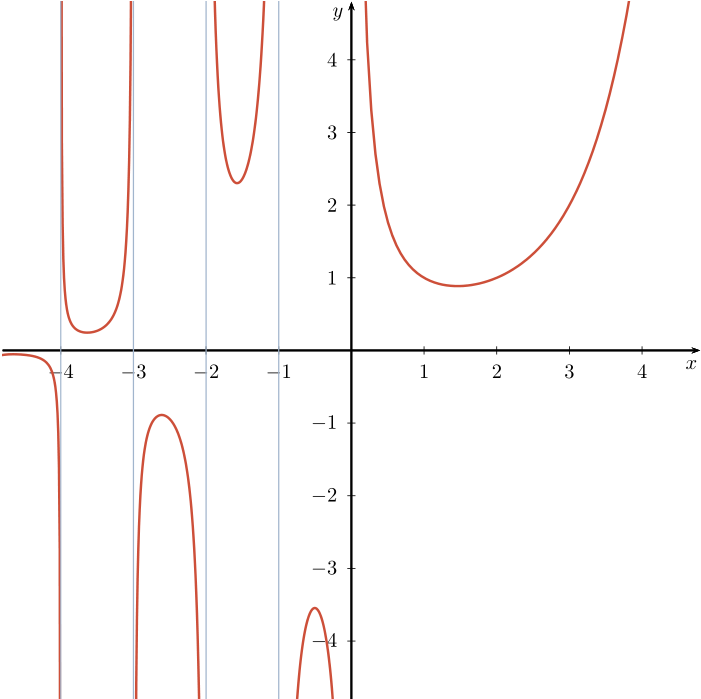
\includegraphics[scale = 0.3]{images/gamma.png}
\end{center}

\section{Gamma distribution} \label{gamma distribution1}
In section \ref{exponential distribution}, we derived the pmf of the exponential distribution by looking at the amount of time leading up to the \textit{first} occurrance in a Poisson distribution. We now do something similar for the gamma distribution. \\

\noindent Let $X \sim$ Poi($\lambda$), where $\lambda$ measures the number of occurrences per 1 second of time. Now define a new random variable, $T$, so that $T$ measures the amount of time leading up to the $k^\text{th}$ occurrence (as opposed to just the first occurrence). Then $T$ is a continuous random variable. \\

\noindent So, we would interpret $P(T > t)$ to be the probability that we have not had $k$ occurrences yet (i.e., that $X < k$) by time $t$. As before, $P(X < k)$, at time $t$, is given by the pmf of Poi($\lambda t$) (see the reasoning behind this in section \ref{exponential distribution}). Furthermore, since $X$ is discrete, we have $P(X < k) = P(X \leq k - 1)$, as $X$ takes no outputs between $k-1$ and $k$. \\

\noindent Let $X \sim $ Poi($\lambda t$). The domain of $X$ is $\set{0,1,2,3,\ldots}$; so,
\begin{align*}
P(X \leq k - 1) & = P(X = 0) + P(X = 1) + \ldots + P(X = k-1) \\
	& = \sum_{\alpha=0}^{k-1}P(X = \alpha) \\
	& = \sum_{\alpha=0}^{k-1}\frac{(\lambda t)^\alpha}{\alpha!}\e^{-\lambda t}. \;\;\;\;\;\;\;\;\; (\dagger) \tag{using the pmf of Poi($\lambda t$), section \ref{lambda poisson}}
\end{align*}

\noindent We now find the cdf, $F(t)$, of $T$, then use this to find the pdf of $T$. We have
\begin{align*}
F(t)   & = P(T \leq t) \tag{definition of a cdf} \\
	& = 1 - P(T > t) \tag{probability measure axiom 1} \\
	& = 1 - P(X < k), \; \text{at time $t$} \tag{by our definition of $T$}  \\
	& = 1 - P(X \leq k-1), \; \text{at time $t$} \tag{since $X$ is discrete} \\
	& = 1 - \sum_{\alpha=0}^{k-1} \frac{(\lambda t)^\alpha}{\alpha!} \e^{-\lambda t } \tag{by ($\dagger$)}
\end{align*}
This is the cdf of the gamma distribution, for $t \geq 0$ (though it is not in a very neat form). To find the pdf, $f(t)$, we differentiate this with respect to $t$. Doing so is not difficult (it involves the product rule and the use of linearity), but there are many steps to simplifying the result, so we will omit the process here (it would be a nice challenging task for the interested reader). The result (after much simplification) is that
\begin{align*}
f(t)  & = \frac{\lambda^\alpha}{(\alpha-1)!}t^{\alpha-1}\e^{-\lambda t} \\
       & = \frac{\lambda^\alpha}{\Gamma(\alpha)}t^{\alpha-1}\e^{-\lambda t} \tag{since $\alpha$ is an integer, so $\Gamma(\alpha) = (\alpha-1)!$}
\end{align*}
Where $t \geq 0$. Replacing the dummy variable, $t$, with $x$, we have the \textbf{pdf of the gamma distribution:} \label{gamma(alpha,lambda)}

  	\bigskip
	
	\hfil\fbox{
	\begin{minipage}{0.65\columnwidth}{
	
	\vskip 0.02cm
	\begin{center}
	$\displaystyle{f(x) = \left\{ \begin{array}{ll}
	\displaystyle{\frac{\lambda^\alpha}{\Gamma(\alpha)}x^{\alpha-1}\e^{-\lambda x}}, & \; \text{if} \; x \geq 0 \smallskip \\ 
	0, & \; \text{if} \; x < 0
	\end{array} \right. }$
	where $\alpha, \lambda > 0$
	\end{center}
	}
	\end{minipage}}
	\bigskip

\noindent The gamma dsitribution takes parameters $\alpha$ and $\lambda$; $\alpha$ is called the \textbf{shape} parameter, and $\lambda$ is called the \textbf{rate}, and some books or software use paremeter $\beta = \frac{1}{\lambda}$, which is called the \textbf{scale} (just as was the case with $\lambda$ in the exponential distribution); hence $\lambda$ is sometimes referred to as the \textbf{inverse scale} parameter. We write \textbf{Gamma($\boldsymbol{\alpha,\lambda}$)} for short. \label{inverse scale gamma} \label{shape gamma} \label{rate gamma} \\

\noindent It is important to emphasize that for a random variable $X \sim $ Gamma($\alpha,\lambda$), the integral
\[
P(a < X < b) = \int_a^b \frac{\lambda^\alpha}{\Gamma(\alpha)}x^{\alpha - 1}\e^{-\lambda x} \; dx 
\]
\textbf{cannot be done exactly}, most of the time. The solutions are generally approximated or looked up using mathematical or statistical software. \\

\noindent Below are some graphs of the gamma distribution for various choices of parameters.
\begin{center}
\begin{tikzpicture}[yscale = 7]
%draw axes
\draw [gray,->] (-0.2,0) -- (7,0) node [below right] {$x$};
\draw [gray,->] (0,-0.2/7) -- (0,1) node [above left] {$f(x)$};
\foreach \y in {0.1,0.2,0.3,0.4,0.5,0.6,0.7,0.8,0.9}{
\draw (0.1,\y) -- (-0.1,\y) node [left] {$\y$}; 
}
\foreach \x in {1,2,3,4,5}{
\draw (\x,0.1/7) -- (\x,-0.1/7) node [below] {$\x$};
}
\draw (4,0.8) node {$\boldsymbol{\lambda = 1}$};
%draw pdfs
\def\alphav{1};
\def\lambdav{1};
\tikzset{declare function={gamma(\z)=(\z-1)!;}}
\def\coefficientv{exp(\alphav*ln(\lambdav))/gamma(\alphav)};
\tikzset{declare function={termone(\x)=exp((\alphav-1)*ln(\x));}}
\tikzset{declare function={termtwo(\x)=exp(-\lambdav*\x);}}
\foreach \t/\colourv in {1/gray,2/red,3/blue,4/black}{
\pgfmathsetmacro\k{\t*20}
\pgfmathsetmacro\l{7/\t}
\pgfmathsetmacro\p{\l-7.5}
\def\alphav{\t};
\draw [very thick,color=\colourv, samples=200,smooth,domain = 0.01:5.5] plot (\x,{\coefficientv*termone(\x)*termtwo(\x)}) node [right = 8mm, below = \p mm] {$\boldsymbol{\alpha = \alphav}$};
}
\end{tikzpicture}
\end{center}
\begin{center}
\begin{tikzpicture}[yscale = 7]
%draw axes
\draw [gray,->] (-0.2,0) -- (7,0) node [below right] {$x$};
\draw [gray,->] (0,-0.2/7) -- (0,1.15) node [above left] {$f(x)$};
\foreach \y in {0.1,0.2,0.3,0.4,0.5,0.6,0.7,0.8,0.9,1,1.1}{
\draw (0.1,\y) -- (-0.1,\y) node [left] {$\y$}; 
}
\foreach \x in {1,2,3,4,5}{
\draw (\x,0.1/7) -- (\x,-0.1/7) node [below] {$\x$};
}
\draw (4,0.8) node {$\boldsymbol{\alpha = 2}$};
%draw pdfs
\def\alphav{2};
\def\lambdav{1};
\tikzset{declare function={gamma(\z)=(\z-1)!;}}
\def\coefficientv{exp(\alphav*ln(\lambdav))/gamma(\alphav)};
\tikzset{declare function={termone(\x)=exp((\alphav-1)*ln(\x));}}
\tikzset{declare function={termtwo(\x)=exp(-\lambdav*\x);}}
\foreach \t/\colourv in {{1/2}/gray,1/red,2/blue,3/black}{
	\pgfmathsetmacro\k{\t*20}
	\pgfmathsetmacro\l{7/\t}
	\pgfmathsetmacro\p{\l-7.5}
	\def\lambdav{\t};
	\draw [very thick,color=\colourv, samples=200,smooth,domain = 0.01:5.5] plot (\x,{\coefficientv*termone(\x)*termtwo(\x)});
}
%labels
\draw (6.3,-0.1/2) node [black] {$\boldsymbol{\lambda = 3}$};
\draw (6.3,0) node [blue] {$\boldsymbol{\lambda = 2}$};
\draw (6.3,0.1/2) node [red] {$\boldsymbol{\lambda = 1}$};
\draw (6.5,0.2/2) node [gray] {$\boldsymbol{\lambda = 1/2}$};
\end{tikzpicture}
\end{center}

\noindent Recall that we derived the pmf of the exponential distribution by looking at the amount of time leading up to the \textit{first} occurrance, i.e. $k = 1$. Since $\alpha$ was our replacement for $k$, we can conclude that Exponential($\lambda$) is a special case of Gamma($\alpha, \lambda$); it is the case with $\alpha = 1$. Indeed, letting $\alpha = 1$ in the pmf of the Gamma distribution gives
\[
f(x) = \frac{\lambda^1}{\Gamma(1)}x^{1-1}\e^{-\lambda x} = \lambda \e^{-\lambda x}.
\]
Which is the pdf of Exponential($\lambda$). \\

\noindent In section \ref{gamma axiom 1}, we will check that the pdf of Gamma($\alpha,\lambda$) satisfies probability measure axiom 1. Then in section \ref{rate/scale gamma}, we will take a deeper look at why $\lambda$ is called the inverse scale parameter.

\section{Memoryless property} \label{memoryless property}
Suppose my friend wants to catch a bus in Japan. When she arrives at the bus stop, the expected wait time is 20 minutes. After 10 minutes, she checks the expected wait time again. Of course, the expected wait time is now 10 minutes. This is an example of a situation where the relevant distribution (of expected waiting times) is not memoryless. \\

\noindent My other friend (I have two) is waiting for a train replacement bus in Melbourne: To begin with, the expected wait time is 20 minutes; 10 minutes later, the expected wait time is 20 minutes; 10 minutes after that, the expected wait time is 20 minutes. This is an example of a situation where the relevant distribution is memoryless. \\

\noindent Only two distributions have the memoryless property: The \textbf{geometric distribution} (discrete) and the \textbf{exponential distribution} (continuous). \\

\noindent Formally, a probability measure has the memoryless property when

  	\bigskip
	
	\hfil\fbox{
	\begin{minipage}{0.45\columnwidth}{
	
	\vskip 0.02cm
	\begin{center}
	$\displaystyle{P(X > a + b \mid X > a) = P(X > b)}$
	\end{center}
	}
	\end{minipage}}
	\bigskip


\subsubsection{Geometric distribution}
\textbf{Proof} \\
Let $X \sim$ Geom($p$). Then,
\begin{align*}
P(X > k) & = 1 - P(X \leq k)  \\
	& = 1 - F(k) \tag{by definition, $F(k) = P(X \leq k)$} \\
	& = 1 - (1-(1-p)^k) \tag{since $F(k) = 1-(1-p)^k$, see section \ref{finite geometric series})} \\
	& = (1-p)^k. \tag{$\bigstar$}
\end{align*}
Now, let $a,b$ be natural numbers. Then
\begin{align*}
P(X > a+b \mid X > a) & = \frac{P(X > a+b \; \textit{and} \; X > a)}{P(X > a)} \tag{dftn of conditional probability} \\
	& = \frac{P(X > a+b)}{P(X > a)} \tag{as $\set{X > a+b} \cap \set{X > a} = \set{X > a+b}$} \\
	& = \frac{(1-p)^{a+b}}{(1-p)^a} \tag{by ($\bigstar$) above} \\
	& = (1-p)^b \tag{index laws} \\
	& = P(X > b).
\end{align*}
Hence $P(X > a+b \mid X > a) = P(X > b)$, which is the definition of the memoryless property, as required. \\

\noindent A famous example (using the geometric distribution) is that of the ``gambler's fallacy.'' Suppose that we are playing roulette, and we are sticking to bets on ``black'' (the probability of landing ``black'' is roughly 47\%). Let $X$ count the number of trials until a win, then $X \sim$ Geom($p$).\\

\noindent Suppose that we bet 7 times in a row, and fail each time. A problem gambler might decide that the odds are now in favour of ``black,'' since the probability of not getting black, so many times in a row, must be very low. The gambler is assuming that
\[
P(X \geq 8 \mid X > 7) \;\;\; \text{is greater than} \;\;\; P(X \geq 1).
\]
But we know, by the memoryless property, that $P(X \geq 7+1 \mid X > 7) = P(X \geq 1)$, which falsifies the gambler's assumption.

\subsubsection{Exponential distribution}
\textbf{Proof} \\
Let $X \sim$ Exponential($\lambda$) and let $a,b$ be natural numbers. Then
\begin{align*}
P(X > a + b \mid X > a) & = \frac{P(X > a + b \; \textit{and} \; X > a)}{P(X > a)} \\
		& = \frac{P(X > a + b)}{P(X > a)} \tag{same reasoning as previous proof} \\
		& = \frac{\e^{-\lambda (a+b)}}{\e^{-\lambda a}} \tag{by result in example \ref{ex17.1}} \\
		& = \e^{-\lambda b} \tag{index laws} \\
		& = P(X > b). \tag{again, by result in example \ref{ex17.1}}
\end{align*}
So the exponential distribution also has the memoryless property, as required.


\chapter{Lecture 18: Antiderivatives of more complicated functions I}
In section \ref{derivativetable1} we developed a small table of antiderivative formulas. Then, in section \ref{Using FTC to find definite integrals}, we learned how to use antiderivatives to find definite integrals.  \\

\noindent In section \ref{product rule} we learned a formula (the ``product rule'') for differentiating functions that can be expressed as a product of two functions. Then, in section \ref{chain rule}, we learned a formula (the chain rule) for differentiating functions which can be expressed as a composition of two functions. These were
\[
\frac{d}{dx}\brac{f(x)g(x)} = f'(x)g(x) + f(x)g'(x) \qquad \text{and} \qquad \frac{d}{dx}\brac{f(g(x))} = f'(g(x))g'(x)
\]

\noindent There are two corresponding antiderivative formulas, one for antidifferentiating products of functions (called \textbf{integration by parts}) and one for antidifferentiating compositions of functions (called \textbf{integration by substitution}); these can be derived from the product and chain rules respectively. \\

\noindent In this lecture we will learn to use integration by parts, and in the next lecture we will learn integration by substitution.

\section{Integration by parts} \label{integration by parts}
Starting from the product rule for derivatives, we can derive the integration by parts rule. The product rule is
\[
\frac{d}{dx}\brac{f(x)g(x)} = f'(x)g(x) + f(x)g'(x)
\]
%Define a new function, $f(x)$, so that $f(x) = k'(x)$. Then $k(x) = \int f(x) \; dx = F(x)$. So we can rewrite the above as
%\[
%\frac{d}{dx}\brac{F(x)g(x)} = f(x)g(x) + F(x)g'(x)
%\]
%Antidifferentiating both sides gives
%\[
%\int\frac{d}{dx}\brac{F(x)g(x)} \; dx = \int f(x)g(x) + F(x)g'(x) \; dx
%\]
%The antiderivative cancels the derivative on the left hand side, and on the right hand side we use linearity, giving
%\[
%F(x)g(x) = \int f(x)g(x) \; dx + \int F(x)g'(x) \; dx
%\]
%Subtracting $ \int F(x)g'(x) \; dx$ from both sides gives us the integration by parts rule:
%
%  	\bigskip
%	
%	\hfil\fbox{
%	\begin{minipage}{0.53\columnwidth}{
%	
%	\vskip 0.02cm
%	\begin{center}
%	$\displaystyle{ \int f(x)g(x) \; dx = F(x)g(x) - \int F(x)g'(x) \; dx}$
%	\end{center}
%	}
%	\end{minipage}}
%	\bigskip
Antidifferentiating both sides gives
\[
\int\frac{d}{dx}\brac{f(x)g(x)} \; dx = \int f'(x)g(x) + f(x)g'(x) \; dx
\]
The antiderivative cancels the derivative on the left hand side, and on the right hand side we use linearity, giving
\[
f(x)g(x) = \int f'(x)g(x) \; dx + \int f(x)g'(x) \; dx
\]
Subtracting $ \int f(x)g'(x) \; dx$ from both sides gives us the integration by parts rule:

  	\bigskip
	
	\hfil\fbox{
	\begin{minipage}{0.53\columnwidth}{
	
	\vskip 0.02cm
	\begin{center}
	$\displaystyle{ \int f'(x)g(x) \; dx = f(x)g(x) - \int f(x)g'(x) \; dx}$
	\end{center}
	}
	\end{minipage}}
	\bigskip

\noindent Another way that it is commonly written is to let $u = f(x)$, and $v = g(x)$; then

  	\bigskip
	
	\hfil\fbox{
	\begin{minipage}{0.4\columnwidth}{
	
	\vskip 0.02cm
	\begin{center}
	$\displaystyle{ \int u'v \; dx = uv - \int uv' \; dx}$
	\end{center}
	}
	\end{minipage}}
	\bigskip

\noindent When using the integration by parts rule, we need to be unusually mindful. If we want to antidifferentiate a product, then we need to nominate one factor to be $f'(x)$, and another factor to be $g(x)$. Looking at the right hand side, this means that we will need to integrate $f'(x)$ to get $f(x)$. Also, we will need to differentiate $g(x)$ to get $g'(x)$. We then need the expression $\int f(x)g'(x) \; dx$ on the far right to be something simpler that can be integrated easier than the expression that we started with; otherwise we end up having to use integration by parts again on $\int f(x)g'(x) \; dx$, which can lead to us being stuck in an endless loop for all eternity. \\

\noindent It is perhaps best taught by example. \\

\noindent A good function to practice on is $h(x) = x\e^{-x}$. Suppose that we haphazardly select $f'(x) = x$ and $g(x) = \e^{-x}$. Then
\[
f(x) = \int x \; dx = \frac{1}{2}x^2 \qquad \text{and} \qquad g'(x) = -\e^{-x}
\]
Now, using integration by parts
\begin{align*}
\int x\e^{-x} \; dx & = f(x)g(x) - \int f(x)g'(x) \; dx \\
		        & = \frac{1}{2}x^2\e^{-x} - \int \frac{1}{2}x^2 (-\e^{-x}) \; dx. \tag{plugging in our results} \\
		        & = \frac{1}{2}x^2\e^{-x} + \frac{1}{2} \int x^2 \e^{-x} \; dx. \tag{linearity}
\end{align*}
We started off needing to integrate $x\e^{-x}$, and now we need to integrate $x^2\e^{-x}$. Things have not gotten any better; they have gotten worse. If we keep going like this, we may never make it out. \\

\noindent We made a mistake, though it is easily fixed by changing our approach. This time we let $f'(x) = \e^{-x}$, and we let $g(x) = x$. Then
\[
f(x) = \int \e^{-x} \; dx = -\e^{-x} \qquad \text{and} \qquad g'(x) = 1
\]
This time, using integration by parts gives
\begin{align*}
\int x\e^{-x} \; dx & = f(x)g(x) - \int f(x)g'(x) \; dx \\
		& = (-\e^{-x})x - \int (-\e^{-x})\times1 \; dx \tag{plugging in our results} \\
		& = -\e^{-x}x + \int \e^{-x} \; dx \tag{linearity} \\
		& = -\e^{-x}x - \e^{-x} \\
		& = -\e^{-x}(x+1).
\end{align*}
This time things went much more smoothly. The trick was to recognise that we would eventually need to integrate a product involving $g'(x)$; letting $g(x) = x$ meant that we would (conveniently) end up integrating a product involving $g'(x) = 1$. 

\subsection{Example}
Find an antiderivative of $x\ln(x)$. \\

\solution
Since we do not even know how to integrate $\ln(x)$ yet (but we do know how to differentiate it), we decide to choose $g(x) = \ln(x)$ and $f'(x) = x$. Then
\[
g'(x) = \frac{1}{x} \qquad \text{and} \qquad f(x) = \int x \; dx = \frac{1}{2}x^2 
\]
Now, using integration by parts
\begin{align*}
\int x\ln(x) \; dx & = f(x)g(x) - \int f(x)g'(x) \; dx	\\
		& = \frac{1}{2}x^2\ln(x) - \int \frac{1}{2}x^2 \frac{1}{x} \; dx \tag{plugging in our results} \\
		& =  \frac{1}{2}x^2\ln(x) - \int \frac{1}{2}x \; dx \\
		& = \frac{1}{2}x^2\ln(x) - \frac{1}{4}x^2 \\
		& = \frac{1}{2}x^2\brac{\ln(x) - \frac{1}{2}}.
\end{align*}

\subsection{Antiderivative of $\boldsymbol{\ln(x)}$}
So far, we know that $\frac{d}{dx}\brac{\ln(x)} = \frac{1}{x}$. However, our table of antiderivatives (given in section \ref{derivativetable1}) does not include a formula for the antiderivative of $\ln(x)$. We now develop one using a clever application of integration by parts. \\

\noindent If we let $g(x) = \ln(x)$, and $f'(x) = 1$, then $\ln(x) = f'(x)g(x)$; this means that we can use integration by parts on $\ln(x)$. We also need the following:
\[
f(x) = \int 1 \; dx = x \qquad \text{and} \qquad g'(x) = \frac{1}{x}.
\]
Using integration by parts we have
\begin{align*}
\int \ln(x) \; dx & = f(x)g(x) - \int f(x)g'(x) \; dx \\
	& = x\ln(x) - \int x\frac{1}{x} \; dx \\
	& = x\ln(x) - \int 1 \; dx \\
	& = x\ln(x) - x.
\end{align*}
We have found a useful antiderivative formula:

  	\bigskip
	
	\hfil\fbox{
	\begin{minipage}{0.35\columnwidth}{
	
	\vskip 0.02cm
	\begin{center}
	$\displaystyle{\int \ln(x) \; dx = x\ln(x) - x}$
	\end{center}
	}
	\end{minipage}}
	\bigskip

\section{Integration by parts with definite integrals} \label{sec18.2}
When using integration by parts on a definite integral, we need to be mindful to think about the terminals. The rule becomes

  	\bigskip
	
	\hfil\fbox{
	\begin{minipage}{0.63\columnwidth}{
	
	\vskip 0.02cm
	\begin{center}
	$\displaystyle{ \int_a^b f'(x)g(x) \; dx = \squac{f(x)g(x)}_a^b - \int_a^b f(x)g'(x) \; dx}$
	\end{center}
	}
	\end{minipage}}
	\bigskip

\noindent For example, suppose we wish to evaluate $\int_0^\infty x\e^{-x} \; dx$. In section \ref{integration by parts} we used integration by parts to find that
\[
\int x\e^{-x} \; dx =  -\e^{-x}x + \int \e^{-x} \; dx 
\]
Adding the terminals we get
\begin{align*}
\int_0^\infty x\e^{-x} \; dx & =  \squac{-\e^{-x}x}_0^\infty + \int_0^\infty \e^{-x} \; dx  \\
		& = 0 + \int_0^\infty \e^{-x} \; dx \tag{since $\e^{-x} \rightarrow 0$ as $x \rightarrow \infty$} \\
		& = \squac{-\e^{-x}}_0^\infty \\
		& = 0 - (-\e^{-0}) \tag{since $\e^{-x} \rightarrow 0$ as $x \rightarrow \infty$} \\
		& = 1. \tag{as $\e^0 = 1$ (index laws)}
\end{align*}

\subsection{Example}
Find $\int_0^3 x^2\e^{-x} \; dx$. \\

\solution
Let $f'(x) = \e^{-x}$ and let $g(x) = x^2$. Then
\[
f(x) = \int \e^{-x} \; dx = -\e^{-x} \qquad \text{and} \qquad g'(x) = 2x
\]
\noindent Using integration by parts,
\begin{align*}
\int_0^3 x^2\e^{-x} \; dx & = \squac{f(x)g(x)}_0^3 - \int_0^3 f(x)g'(x) \; dx \\
	& = \squac{-\e^{-x}x^2}_0^3 - \int_0^2 (-\e^{-x})2x \; dx \tag{plugging in our results} \\
	& = \squac{-\e^{-x}x^2}_0^3 + 2\int_0^2 \e^{-x}x \; dx \tag{linearity} \\
	& = \squac{-\e^{-x}x^2}_0^3 + 2\squac{-\e^{-x}(x+1)}_0^3 \tag{by the result in section \ref{integration by parts}} \\
	& = -\e^{-3}3^2 - 0 + 2\brac{-\e^{-3}(3+1) - (-1)} \\
	& = 2 - 17\e^{-3}.
\end{align*}

\section{Proofs for some properties of the gamma function} \label{sec18.1}
\subsubsection{Proof that $\boldsymbol{\Gamma(\alpha) = (\alpha-1)\Gamma(\alpha-1)}$} 
In section \ref{gamma properties} we mentioned this important property of the gamma function. Now we can prove it using integration by parts: \\

\noindent By definition, the gamma function is
\[
\Gamma(\alpha) = \int_0^\infty x^{\alpha - 1}\e^{-x} \; dx
\]
Let $f'(x) = \e^{-x}$ and let $g(x) = x^{\alpha - 1}$. Then
\[
f(x) = \int \e^{-x} \; dx = -\e^{-1} \qquad \text{and} \qquad g'(x) = (\alpha - 1)x^{\alpha - 2}.
\]
Now, using integration by parts gives
\begin{align*}
\Gamma(\alpha) & = \squac{f(x)g(x)}_0^\infty - \int_0^\infty f(x)g'(x) \; dx \\
	& = \squac{-\e^{-x}x^{\alpha - 1}}_0^\infty + (\alpha - 1)\int_0^\infty \e^{-x}x^{\alpha - 2} \; dx \tag{using linearity}\\
	& = 0 + (\alpha - 1)\int_0^\infty e^{-x}x^{\alpha - 2} \; dx \tag{since $\e^{-x} \rightarrow 0$ as $x \rightarrow \infty$} \\
	& = (\alpha - 1)\Gamma(\alpha - 1). \tag{definition of gamma function}
\end{align*}
Which is what we wanted to show.

\subsubsection{Proofs that $\boldsymbol{\Gamma(1) = 1}$ and $\boldsymbol{\Gamma(n) = (n-1)!}$ for $\boldsymbol{n \in \N}$}
By the definition of the gamma function we have
\[
\Gamma(2) = \int_0^\infty x^{2-1}\e^{-x} \; dx = \int_0^\infty x\e^{-x} \; dx
\]
We evaluated this integral in \ref{sec18.2}; we found that $\int_0^\infty x\e^{-x} \; dx = 1$. Hence,
\[
\Gamma(2) = 1.
\]
Using the fact that 
\[
\boldsymbol{\Gamma(\alpha) = (\alpha - 1)\Gamma(\alpha - 1)} \tag{$\bigstar$}
\]
we have
\[
\Gamma(2) = (2-1)\Gamma(2-1) = \Gamma(1)
\]
So $\Gamma(1) = 1$ as well. \\

\noindent Now, let $n$ be a natural number. For the following steps we just use $\bigstar$ repeatedly:
\begin{align*}
\Gamma(n) & = (n-1)\Gamma(n-1)  \tag{by $\bigstar$} \\
	& = (n-1)(n-2)\Gamma(n-2) \tag{as $\Gamma(n-1) = (n-2)\Gamma(n-2)$} \\
	& = (n-1)(n-2)(n-3)\Gamma(n-3)  \tag{as $\Gamma(n-2) = (n-3)\Gamma(n-3)$}\\
	& = \ldots \tag{continue applying $\bigstar$ repeatedly} \\
	& = (n-1)(n-2)(n-3)\times\ldots\times\Gamma(3) \\
	& = (n-1)(n-2)(n-3)\times\ldots\times2\Gamma(2) \tag{as $\Gamma(3) = 2\Gamma(2)$} \\
	& = (n-1)(n-2)(n-3)\times\ldots\times2\times1\times\Gamma(1). \tag{as $\Gamma(2) = 1\Gamma(1)$} \\
	& = (n-1)!  \tag{as $\Gamma(1) = 1$}
\end{align*}
Hence $\Gamma(n) = (n-1)!$, as required.


\chapter{Lecture 19: Antiderivatives of more complicated functions II}
In the previous lecture we introduced integration by parts, as the antiderivative analogue of the product rule. Now we introduce integration by substitution. \\

\noindent Integration by substitution is the antiderivative analogue of the chain rule. We can use it to integrate functions which involve compositions of two functions. However, we will soon see that the types of functions that we can integrate by substitution need to satisfy some extra conditions (they do not only involve compositions).

\section{Integration by substitution} \label{integration by substitution 1}
We now derive the integration by substitution rule from the chain rule. For the product rule, our notation involved using $f(x)$ and $f'(x)$, where $f(x)$ was an antiderivative of $f'(x)$. To make the integration by substitution rule neater we will use $F(x)$ and $f(x)$, where $F(x)$ is an antiderivative of $f(x)$; both ways mean the same thing, it is just a matter of preference in notation. \\

\noindent The chain rule is
\[
\frac{d}{dx}\brac{F(g(x))} = f(g(x))g'(x)
\]
Integrating both sides gives
\[
\int \frac{d}{dx}\brac{F(g(x))} \; dx = \int f(g(x))g'(x) \; dx
\]
The antiderivative cancels the derivative on the left hand side, giving the integration by substitution rule (we also swapped the sides of the equality):

  	\bigskip
	
	\hfil\fbox{
	\begin{minipage}{0.35\columnwidth}{
	
	\vskip 0.02cm
	\begin{center}
	$\displaystyle{\int f(g(x))g'(x) \; dx = F(g(x))}$
	\end{center}
	}
	\end{minipage}}
	\bigskip

\noindent Sometimes you will see this written differently, as follows: If we let $g(x) = u$, then $g'(x) = \frac{du}{dx}$, and $F(g(x)) = F(u)$. So we write

  	\bigskip
	
	\hfil\fbox{
	\begin{minipage}{0.35\columnwidth}{
	
	\vskip 0.02cm
	\begin{center}
	$\displaystyle{\int f(u)\frac{du}{dx} \; dx = F(u)}$
	\end{center}
	}
	\end{minipage}}
	\bigskip

\noindent There is another very common way to write it, which may help with your understanding and memory, so we have to include it here. It is important to realise that $F(u)$ really means ``the antiderivate of $f(u)$,'' i.e., $F(u) = \int f(u) \; du$. Hence you will often see the integration by substitution rule written:

  	\bigskip
	
	\hfil\fbox{
	\begin{minipage}{0.35\columnwidth}{
	
	\vskip 0.02cm
	\begin{center}
	$\displaystyle{\int f(u)\frac{du}{dx} \; dx = \int f(u) \; du}$
	\end{center}
	}
	\end{minipage}}
	\bigskip

\noindent To help remember this rule, people imagine that they are ``cancelling the $dx$'' from the right hand side, so they pretend that $\displaystyle{\frac{du}{dx}dx = du}.$ \\

\noindent Just to throw in one more way to write it, a personal favourite is

  	\bigskip
	
	\hfil\fbox{
	\begin{minipage}{0.4\columnwidth}{
	
	\vskip 0.02cm
	\begin{center}
	$\displaystyle{\int f(g(x))g'(x) \; dx = \int f(u) \; du}$, where $u = g(x).$
	\end{center}
	}
	\end{minipage}}
	\bigskip

\noindent At first it is troubling having so many ways to write the same thing, then it eventually becomes useful to have some freedom of expression. The important thing is that we understand exactly what the rule is saying. \\

\noindent Usually, we apply this rule by trying to match the left hand side of the rule to the function that we are integrating. So, we need to pick $g(x)$ and $f(x)$ in such a way that the function we are integrating has the form $f(g(x))g'(x)$; or, if you like the other notation better: $f(u)\frac{du}{dx}.$ \\

\noindent As you can see, this form is not simply a ``composition of two functions;'' it is also the product of that composition with the derivative of the inner function, $g(x)$. \\

\noindent For example, the function $h(x) = x\e^{-\frac{1}{2}x^2}$ has the required form: Where $f(x) = \e^{-x}$ and $g(x) = \frac{1}{2}x^2$. So, $f(g(x)) = \e^{-\frac{1}{2}x^2}$ and $g'(x) = \frac{2}{2}x = x$, giving
\[
f(g(x))g'(x) = x\e^{-\frac{1}{2}x^2} = h(x)
\]
This means that
\begin{align*}
\int x\e^{-\frac{1}{2}x^2} \; dx & = \int f(g(x))g'(x) \; dx \\
	& =  \int f(u) \; du   \tag{substitution rule, where $u = g(x)$}\\
	& = \int \e^{-u} \; du \tag{since $f(x) = \e^{-x}$} \\
	& = -\e^{-u} \\
	& = -\e^{-\frac{1}{2}x^2}. \tag{since $u = g(x) = \frac{1}{2}x^2$}
\end{align*}
The function that we just integrated may have looked like a good candidate for integration by parts. However, using integration by parts on this function will lead to problems (try it). A good rule of thumb is to always decide if you can apply integration by substitution first, then use integration by parts otherwise.

\subsection{The simplest type of substitution}
We gave a rule in section \ref{simplest chain} for the simplest application of the chain rule, we now give a rule for the simplest application of substitution. \\

\noindent Just as was the case with the chain rule, the simplest type of substitution is when
\[
h(x) = f(ax+b), \qquad \text{for any real constants $a,b.$}
\] 
We can let $f(ax+b) = f(g(x))$, where $g(x)$ has the form of a straight line, i.e., $g(x) = ax+b$. So,
\[
g'(x) = \frac{d}{dx}\brac{ax+b} = a.
\]
To match the left hand side of the substitution rule, the function we are integrating must have the form $g'(x)f(g(x))$, which in this case would look like
\[
g'(x)f(g(x)) = af(ax+b). \tag{since $g'(x) = a$}
\]
But $h(x) = f(ax+b)$, not $af(ax+b)$; there is no constant, $a$, out front yet. However, multiplying by $\frac{a}{a} = 1$ will fix this, without changing the value of the expression (we are technically just multiplying by 1). Doing this, then using the linearity of integration
\[
\int f(ax+b) \; dx = \int\frac{a}{a} f(ax+b) \; dx = \frac{1}{a} \int af(ax+b) \; dx.
\]
We have
\begin{align*}
\int f(ax+b) \; dx & = \frac{1}{a} \int af(ax+b) \; dx \\
	& = \frac{1}{a} \int g'(x)f(g(x)) \; dx \tag{since $g(x) = ax+b$ and $g'(x) = a$} \\
	& = \frac{1}{a} F(u) \qquad (\bigstar) \tag{letting $u = g(x)$, integration by substitution} \\
	& = \frac{1}{a} \int f(u) \; du. \tag{since $F$ is an antiderivative of $f$}
\end{align*}
Where $u = ax+b$. \\

\noindent For example. Suppose we wish to antidifferentiate $h(x) = (3x+12)^8$. Then $u = 3x+12$, $f(u) = u^8$, and $a = 3$. So $(\bigstar)$ tells us that
\begin{align*}
\int (3x+12)^8 \; dx & = \frac{1}{3} \int f(u) \; du \\
	& = \frac{1}{3} \int u^8 \; du \tag{since $f(u) = u^8$} \\
	& = \frac{1}{3} \frac{1}{9}u^9 \tag{integration formula} \\
	& = \frac{1}{27} (3x+12)^9. \tag{since $u = 3x+12$}
\end{align*}
In practice, you can skip many of the explanatory steps and just ``write down'' the answer once you get used to simple substitution.

\subsection{Simple substitution with integration by parts}
Suppose we wish to antidifferentiate the function $h(x) = x(x+2)^9$. A clever substitution could achieve this (see below), however we can also do it by brute force as follows. If we choose $g(x) = x$ and $f'(x) = (x+2)^9$, then integration by parts will work. To integrate $f'(x)$ we need to use simple substitution, with $a = 1$ and $f(u) = u^9$. Then we get
\[
g'(x) = 1 \qquad \text{and} \qquad f(x) = \int f'(x) \; dx = \frac{1}{10}(x+2)^{10}.
\]
Now, using integration by parts
\begin{align*}
\int x(x+2)^9 & = f(x)g(x) - \int f(x)g'(x) \; dx \\
	& = \frac{1}{10}(x+2)^{10}x -  \frac{1}{10} \int (x+2)^{10} \; dx \tag{linearity}
\end{align*}
For the integral on the right hand side, we need to use simple substitution again, with $a = 1$ and $f(u) = u^{10}$. This gives $\int (x+2)^{10} \; dx = \frac{1}{11}(x+2)^{11}$. So,
\begin{align*}
\int x(x+2)^9 & =  \frac{1}{10}(x+2)^{10}x -  \frac{1}{10}\brac{\frac{1}{11} (x+2)^{11}} \; dx \\
	& = \frac{x}{10}(x+2)^{10} - \frac{1}{110}(x+2)^{11}.
\end{align*}
We could probably simplify this, but it is ok to stop here.

\subsubsection{A clever substitution}
There is a nicer, trickier way to integrate $h(x) = x(x+2)^9$, that reveals some of the hidden powers of substitution. You will not be required to use substitution in this way, during this course; though you might encounter situations where you \textit{can} use it if you wish. Let  $g(x) = x+2$, then $g'(x) = 1$. Also let $u = g(x)$ so $u = x+2$. Then $x = u - 2$ (solving for $x$). So we can rewrite:
\[
x(x+2)^9 = (u-2)u^9 \tag{where $u = x+2$}
\]
If we now let $f(g(x)) = f(u) = (u-2)u^9$, then we have
\[
h(x) = f(g(x)). \tag{where $g(x) = x+2$}
\]
And since $g'(x) = 1$ we have $h(x) = f(g(x)) = f(g(x))g'(x)$ (multiplying by 1).
Now the great thing about our expression for $f(u)$ is that it does not have a binomial power anymore (expanding $(x+2)^9$ would have been difficult). Now we can expand the brackets easily, and the resulting term can be integrated using linearity. We have,
\[
f(u) = (u-2)u^9 = u^{10} - 2u^9. \tag{expanding the brackets}
\]
Now,
\begin{align*}
\int x(x+2)^9 \; dx & = \int f(g(x))g'(x) \; dx \\
	& = \int f(u) \; du  \tag{integration by substitution} \\
	& = \int u^{10} - 2u^9 \; du \\
	& = \frac{1}{11}u^{11} - \frac{2}{10}u^{10} \tag{linearity} \\
	& = \frac{1}{11}(x+2)^{11} - \frac{2}{10}(x+2)^{10}
\end{align*}
It can be shown that this answer is equal to the result that we obtained using integration by parts (it just needs to be rearranged).

\subsection{Example}
Find an antiderivative of $\displaystyle{h(x) = \frac{x^2}{1+x^3}}$, using integration by substitution. \\

\solution
Let $f(u) = \frac{1}{u}$, with $u = g(x) = 1 + x^3$. Then $g'(x) = 3x^2$. So,
\[
f(g(x))g'(x) = \frac{1}{1+x^3}\times3x^2 = 3 \frac{x^2}{1+x^3}.
\]
It follows that
\[
h(x) = \frac{x^2}{1+x^3} = \frac{1}{3}\brac{3 \frac{x^2}{1+x^3}} = \frac{1}{3}f(g(x))g'(x). 
\]
Now we can use linearity to get
\begin{align*}
\int h(x) \; dx & = \frac{1}{3}\int f(g(x))g'(x) \; dx \\
		& = \frac{1}{3}\int f(u) \; du \tag{integration by substitution} \\
		& = \frac{1}{3}\int \frac{1}{u} \; du \\
		& = \frac{1}{3}\ln(u) \tag{integration formula} \\
		& = \frac{1}{3}\ln(1 + x^3). \tag{as $u = 1+ x^3$}
\end{align*}

\section{Substitution with definite integrals} \label{subst definite}
As with integration by parts, we can use integration by substitution on definite integrals as long as we are careful to remember the terminals. The rule becomes:

  	\bigskip
	
	\hfil\fbox{
	\begin{minipage}{0.45\columnwidth}{
	
	\vskip 0.02cm
	\begin{center}
	$\displaystyle{\int_{u(a)}^{u(b)} f(u) \; du = \int_a^b f(g(x))g'(x) \; dx,}$ where $u = g(x)$.
	\end{center}
	}
	\end{minipage}}
	\bigskip

\noindent Notice that the terminals on the left hand side are not simply $a$ and $b$; they are $u(a)$ and $u(b)$, i.e.,  they are $g(a)$ and $g(b)$ respectively. This makes sense because on the right hand side we integrate with respect to $x$ (the terminals on the right hand side represent points on an $x$-axis), while on the left hand side we integrate with respect to $u$ (the terminals on the left hand side represent points on a $u$-axis). It is not necessary to think too hard about the abstract idea of a ``$u$-axis;'' you just need to recognise that when we integrate with respect to $u$, the terminals must also be ``with respect to $u$.'' \\

\noindent We now demonstrate how to use this rule, by example. Suppose we wish to evaluate
\[
\int_0^4 x\e^{-\frac{x^2}{2}} \; dx
\]
At the end of section \ref{integration by substitution 1} we found that
\[
\int x\e^{-\frac{1}{2}x^2} \; dx = -\e^{-u} \tag{where $u = \frac{1}{2}x^2$}
\]
Adding in the terminals we get
\[
\int_0^4 x\e^{-\frac{1}{2}x^2} \; dx = \squac{-\e^{-u}}_{u(0)}^{u(4)}
\]
Now, $u(0) = \frac{1}{2}(0)^2 = 0$, and $u(4) = \frac{1}{2}4^2 = 8$. So,
\begin{align*}
\int_0^4 x\e^{-\frac{1}{2}x^2} \; dx & = \squac{-\e^{-u}}_0^8 \\\
	& = -\e^{-8} - (-\e^{0}) \\
	& = 1 - \e^{-8}.
\end{align*}

\subsection{Example}
Evaluate the following using integration by substitution:
\[
\int_{-1}^1 4x^3\e^{1-x^4} \; dx.
\]

\solution
Let $f(u) = \e^u$ and let $u = g(x) = 1-x^4$. Then $g'(x) = 4x^3$. So,
\[
4x^3\e^{1-x^4} = f(g(x))g'(x).
\]
Hence, using integration by substitution we have
\begin{align*}
\int_{-1}^1 4x^3\e^{1-x^4} \; dx  & = \int_{u(-1)}^{u(1)} f(u) \; du \\
	& = \int_{u(-1)}^{u(1)} \e^u \; du
\end{align*}
Now, since $u = 1-x^4$, we have $u(-1) = 1 - (-1)^4 = 0$ and $u(1) = 1 - 1^4 = 0$, so
\[
\int_{-1}^1 4x^3\e^{1-x^4} \; dx = \int_{0}^{0} \e^u \; du = 0.
\]

\section{Right-to-left substitution} \label{right-to-left substitution}
So far, in this lecture, we have have used substitution by first matching our function to the left hand side of the substitution rule, $f(g(x))g'(x)$; we call this, ``\textbf{left-to-right}'' substitution.
\begin{center}
\begin{tikzpicture}
\draw (0,0) node {$\displaystyle{\int f(g(x))g'(x) \; dx = \int f(u) \; du}$};
\draw [gray!110] (0,-0.8) node {Left-to-right};
\draw [gray!110] (0,-1.2) node {$\longrightarrow$};
\draw [gray!110] (4,-1) node {where $u = g(x)$};
\end{tikzpicture}
\end{center}
Sometimes it is useful to work ``\textbf{right-to-left}'' instead. 
\begin{center}
\begin{tikzpicture}
\def\x{-1.1};
\draw (0+\x,0) node {$\displaystyle{\int f(g(u))g'(u) \; du = \int f(x) \; dx}$};
\draw [gray!110] (0+\x,-0.8) node {Right-to-left};
\draw [gray!110] (0+\x,-1.2) node {$\longleftarrow$};
\draw [gray!110] (4+\x,-1) node {where $x = g(u)$};
\draw (-6,-1.7) -- (6,-1.7) -- (6,1) -- (-6,1) -- cycle;
\end{tikzpicture}
\end{center}
In right-to-left substitution, we first match our function to the expression on the right hand side. This time, instead of having $u = g(x)$, we have $x = g(u)$; i.e., $x$ is a function of $u$ now, so we can write $x(u)$ and $x'(u)$ (treating $x$ as a function) the same way we would have written $u(x)$ and $u'(x)$ when we did left-to-right substitution (when $u$ was a function of $x$). So, another way to write the right-to-left substitution rule is
\[
\int f(x(u))x'(u) \; du = \int f(x) \; dx
\]
Or another alternative notation is
\[
\int f(x(u))\frac{dx}{du} \; du = \int f(x) \; dx
\]
Again, the way we write it isn't important as long as we understand what the rule is saying. Also keep in mind that, really, left-to-right and right-to-left substitution are the same rule, we just write them differently because we use them differently (we like to have the $u$ on the side that we are moving towards).

\subsubsection{Example: proof of antiderivative of $\boldsymbol{\frac{1}{x}}$}

\noindent In section \ref{log no proof}, we stated that $\frac{d}{dx}\brac{\ln(x)} = \frac{1}{x}$, then we used this claim in section \ref{derivativetable1} to show that $\int \frac{1}{x} \; dx = \ln(x)$. We still have not proven the original claim. \\

\noindent We now present a proof that $\int \frac{1}{x} \; dx = \ln(x)$, as an easy example of right-to-left substitution; the fact that $\frac{d}{dx}\brac{\ln(x)} = \frac{1}{x}$ then follows naturally, since integration (i.e., antidifferentiation) is inverse to differentiation. \\ 

\noindent This proof only uses the derivative of $\e^x$ and the fact that $\ln(x)$ is inverse to $\e^x$. \\

\noindent Let $f(x) = \frac{1}{x}$ and let $x = g(u) = \e^u$. Then
\[
g'(u) = \frac{d}{du}\brac{\e^u} = \e^u \qquad \text{and} \qquad f(g(u)) = \frac{1}{\e^u}. 
\]
Also, since $x = \e^u$, it follows that $u = \ln(x)$ (taking natural log of both sides, since natural log is inverse to exponential). Now,
\begin{align*}
\int \frac{1}{x} \; dx & = \int f(x) \; dx \tag{as $f(x) = \frac{1}{x}$} \\
	& = \int f(g(u))g'(u) \; du \tag{integration by substitution (right-to-left)} \\
	& = \int \frac{1}{\e^u} \e^u \; du \tag{plugging in our results: $f(g(u)) = \frac{1}{\e^u}$ and $g'(u) = \e^u$} \\
	& = \int 1 \; du \\
	& = u \tag{since we are integrating with respect to $u$}\\
	& = \ln(x). \tag{since $u = \ln(x)$}
\end{align*}

\section{Right-to-left substitution with definite integrals}
In section \ref{subst definite} we learned about left-to-right substitution with definite integrals. We had $u = g(x)$, and the terminals on the left hand side were $a$ and $b$. However, in right-to-left substitution we have $x = g(u)$, and we choose to label the terminals on the right $a$ and $b$. To understand it right-to-left we can write the substitution rule as:
\begin{center}
\begin{tikzpicture}
\def\x{-1.1};
\draw (0+\x,0) node {$\displaystyle{\int_{g^{-1}(a)}^{g^{-1}(b)} f(g(u))g'(u) \; du = \int_a^b f(x) \; dx}$};
\draw [gray!110] (0+\x,-0.8) node {Right-to-left};
\draw [gray!110] (0+\x,-1.2) node {$\longleftarrow$};
\draw [gray!110] (4+\x,-1) node {where $x = g(u)$};
\draw (-6,-1.7) -- (6,-1.7) -- (6,1) -- (-6,1) -- cycle;
\end{tikzpicture}
\end{center}
Once we move to the left, we need the terminals to be ``in terms of'' $u$. Since we defined $x = g(u)$, it follows that $u = g^{-1}(x)$, which is why we are using the inverse of $g$ to obtain terminals in terms of $u$. So, for example, if $x = g(u) = u + 2$, then $u = g^{-1}(x) = x - 2$ (solving for $x$). \\

\noindent In the following two sections we will use right-to-left substitution on definite integrals.
\section{Checking that the pdf of Gamma($\boldsymbol{\alpha,
\lambda}$) satisfies axiom 1} \label{gamma axiom 1}
In section \ref{pdf} we stated two conditions that need to be checked for pdfs, which are equivalent to checking probability measure axioms 1 and 2. It is easy to check that the outputs of the pdf are all positive, so we wont check that here; we just check axiom 1. We will do this using right-to-left substitution. The pdf of the gamma distribution is
\[
f(x) = \left\{ \begin{array}{ll}
\frac{\lambda^\alpha}{\Gamma(\alpha)}x^{\alpha - 1}\e^{-\lambda x} \; dx, & \; \text{if} \; x \geq 0 \smallskip \\
0, & \; \text{if} \; x < 0
\end{array}
\right.
\]
Hence we have
\[
\int_{-\infty}^\infty f(t) \; dt = \int_{0}^\infty \frac{\lambda^\alpha}{\Gamma(\alpha)}t^{\alpha - 1}\e^{-\lambda t} \; dt \tag{since $f(x) = 0$ for $x < 0$}.
\]
Let $f(x)$ be the pdf of the gamma distribution, and let $t = g(u) = \frac{u}{\lambda}$. Then $g'(u) = \frac{1}{\lambda}$ (since $\frac{1}{\lambda}$ is just a constant). Also, we can solve for $u$ in $t = \frac{u}{\lambda}$ to get $g^{-1}(t) = u = \lambda t$. \\

\noindent Now, when we do the substitution, we have to think about the terminals: Since $u = g^{-1}(t) = \lambda t$, we can see that $u \rightarrow \infty$ as $t \rightarrow \infty$ and $u = 0$ when $t = 0$, so in this case the terminals do not change when we do the substitution: 
\begin{align*}
\int_{-\infty}^\infty f(t) \; dt & = \int_0^\infty f(g(u))g'(u) \; du \tag{substitution right-to-left} \\
	& = \int_0^\infty \frac{\lambda^\alpha}{\Gamma(\alpha)}\brac{\frac{u}{\lambda}}^{\alpha - 1} \e^{-u} \frac{1}{\lambda} \; du \tag{since $g'(u) = \frac{1}{\lambda}$ and $g(u) = \frac{u}{\lambda}$} \\
	& = \int_0^\infty \frac{\lambda^\alpha}{\Gamma(\alpha)}\frac{1}{\lambda}\frac{u^{\alpha - 1}}{\lambda^{\alpha - 1}} \e^{-u} \; du  \tag{index laws, and rearranging} \\
	& = \int_0^\infty \frac{\lambda^\alpha}{\Gamma(\alpha)}\frac{1}{\lambda^\alpha} u^{\alpha - 1} \e^{-u} \; du  \tag{index laws, i.e., $\frac{1}{\lambda}\frac{1}{\lambda^{\alpha - 1}} = \frac{1}{\lambda^\alpha}$} \\
	& = \frac{1}{\Gamma(\alpha)} \int_0^\infty u^{\alpha - 1} \e^{-u} \; du  \tag{cancelling the two $\lambda^\alpha$ and using linearity} \\
	& = \frac{1}{\Gamma(\alpha)}\Gamma(\alpha) \tag{definition of the gamma function} \\
	& = 1.
\end{align*}
So $\int_{-\infty}^\infty f(t) \; dt = 1,$ as required. \\

\noindent Notice that the choice of substitution, $t = \frac{u}{\lambda}$, generated a factor of $1/\lambda^\alpha$, which resulted in the powers of $\lambda$ cancelling eachother out. In general, for the above integral, a substitution of $t = cu$, for any positive real number choice of $c$, will produce a factor of $c^\alpha$. The powers of $\lambda$ don't cancel unless $c = \frac{1}{\lambda}$, but we can still use index laws to bring $\lambda$ and $c$ together as $c^\alpha \lambda^\alpha = \brac{c \lambda}^\alpha$. \\

\noindent We will see this in action in the next section when look at why $\lambda$ is called the ``inverse scale parameter.''
%, and $\e^{-\lambda t}$ become $\e^{-\frac{\lambda}{c}u}$. This is the reason that we name $\lambda$ the ``inverse scale parameter''; we discuss this further in the next section. 

\section{Random variables and scale} \label{rate/scale gamma} \label{scale - actual description}
Suppose we have one random variable, $X$, and we wish to define another random variable, $Y$, using $X$. Recall that random variables are fuctions whose domain is the outcome space, and whose range is some subset of the real numbers. The possible outputs of $Y$ are represented by  $y$, and the possible outputs of $X$ are represented by $x$. In section \ref{def Y = g(X)} we will look at defining one variable in terms of another variable, more generally. For now, we will just look at the case, $Y = \frac{X}{c}$. Let $c$ be a positive real number. If we write $Y = \frac{X}{c}$, we mean that we take each individual output, $x$, of $X$, and from each of these obtain each output, $y$, of $Y$, by letting $y = \frac{x}{c}$.
\begin{center}
\begin{tikzpicture}
%outcome space
\draw (-6,0) circle (2cm);
\draw (-6,-2.3) node {$\boldsymbol{\Omega}$\textbf{ (outcome space)}};
\draw [fill = black] (-5,1) circle (0.04cm) node [above] {$\omega_1$};
\draw [fill = black] (-7,0) circle (0.04cm) node [above] {$\omega_2$};
\draw [fill = black] (-5.5,-1) circle (0.04cm) node [above] {$\omega_3$};

%range of X
\draw (0,0) circle (2cm);
\draw (0,-2.3) node {\textbf{Range of $\boldsymbol{X}$}};
\draw [fill = black] (0,1) circle (0.04cm) node [above] {$x_1$};
\draw [fill = black] (0.3,-1) circle (0.04cm) node [above] {$x_2$};

%range of Y
\draw (6,0) circle (2cm);
\draw (6,-2.3) node {\textbf{Range of $\boldsymbol{Y}$}};
\draw [fill = black] (6.7,0.5) circle (0.04cm) node [above] {$y_1$};
\draw [fill = black] (5.7,-0.7) circle (0.04cm) node [above] {$y_2$};

%ARROWS
%from Omega to X
\draw [gray!120, -latex] (-5,1) -- (-0.1,1);
\draw [gray!120, -latex] (-7,0) -- (-0.1,0.94);
\draw [gray!120, -latex] (-5.5,-1) -- (0.26,-1);
%from X to Y
\draw [gray!120, -latex] (0,1) -- (6.5,0.5) node [above, midway] {$y_1 = x_1/c$};
\draw [gray!120, -latex] (0.3,-1) -- (5.5,-0.7) node [above, midway] {$y_2 = x_2/c$};

%curvy arrows
\draw [gray!120, ->] (-4,2) [out=10, in =170] to (-2,2);
\draw (-3,2.4) node {$X(\omega)$};

\draw [gray!120, ->] (2,2) [out=10, in =170] to (4,2);
\draw (3,2.4) node {$Y = \frac{X}{c}$};

\end{tikzpicture}
\end{center}




\noindent So, for example, if $X = 1$, then $Y = \frac{1}{c}$, or if $X = 2.4$, then $Y = \frac{2.4}{c}$. In this way, $\set{X = a}$, for some $a$, will refer to one subset of the outcome space (i.e., one event), and consequently $\set{Y = \frac{a}{c}}$, will refer to \textit{the same} event. So, in the above graph we have $\set{Y = y_2} = \set{\omega_3}$ and $\set{Y = y_1} = \set{\omega_1,\omega_2}$. If you are having trouble thinking of random variables as functions whose domain is the outcome space, then review section \ref{sec8.10}. \\

\noindent For example, suppose that $X$ measures, in centimeters, the level of water in a reservoir after a period of rainfall. Then the event $X = 200$ corresponds to a depth of 200cm. Now, define $Y = \frac{X}{100}$. Then, when $X = 200$ we have $Y = \frac{200}{100} = 2$ units. The units of $Y$ are not centimeters, since $X = 200$ and $Y = 2$ both refer to the \textit{same event} (i.e., the same depth). There are 100 centimeters in a meter, so the units of $Y$ are meters; the water is 200cm, i.e., 2 meters, deep. The depth of the water is the same in both cases, we are just looking at it on a different \textbf{scale}; that is, $Y$ is just a \textbf{rescaled} version of $X$. \\

\noindent Now, suppose we have $X \sim$ Gamma($\alpha,\lambda$), and we define $Y = \frac{X}{c}$. Then what is the distribution of $Y$? We claim that $Y \sim$ Gamma($\alpha,c\lambda$). That is, we claim that rescaling $X$, to create $Y$, only affects the ``inverse scale parameter,'' $\lambda$; this would justify the use of the word, ``scale,'' in the naming of $\lambda$. In lecture 21 we will learn about the ``method of distributions,'' which will allow us to prove this fact, in section \ref{ex21.1}. \\

\noindent Indeed, if $X \sim$ Gamma($\alpha,\lambda$), and $Y = \frac{X}{c}$. Then $y = \frac{x}{c}$ so let $x = g(y) = cy$ (solving for $x$). So, we have $g'(y) = \frac{dx}{dy} = \frac{d}{dy}\brac{cy} = c$. Hence, we can use right-to-left substitution, almost the same as we did in section \ref{gamma axiom 1}:
\begin{align*}
P(a < X < b) & = \int_a^b \frac{\lambda^\alpha}{\Gamma(\alpha)}x^{\alpha - 1} \e^{-\lambda x} \; dx \tag{By the pdf for $X$} \\
	& = \int_{g^{-1}(a)}^{g^{-1}(b)} \frac{\lambda^\alpha}{\Gamma(\alpha)}(cy)^{\alpha - 1} \e^{-\lambda (cy)} \; \frac{dx}{dy} \; dy \tag{substitution with $x = g(y) = cy$}
\end{align*}
We had $x = g(y) = cy$, so $y = g^{-1}(x) = \frac{x}{c}$. Thus the terminals are $g^{-1}(a) = \frac{a}{c}$ and $g^{-1}(b) = \frac{b}{c}.$ Plugging these in gives
\begin{align*}
P(a < X < b) & = \int_{a/c}^{b/c} \frac{\lambda^\alpha}{\Gamma(\alpha)}(cy)^{\alpha - 1} \e^{-\lambda (cy)} \; c \; dy \tag{as $\frac{dx}{dy} = c$} \\
	& = \int_{a/c}^{b/c} \frac{\lambda^\alpha}{\Gamma(\alpha)} c^\alpha y^{\alpha - 1} \e^{-(c \lambda) y} \; dy \tag{bringing together all the factors of $c$} \\
	& =  \int_{a/c}^{b/c} \frac{(c \lambda)^\alpha}{\Gamma(\alpha)} y^{\alpha - 1} \e^{-(c \lambda)y} \; dy \;\;\;\;\;\;\;\;\;\;\;\; (\bigstar) \tag{since $c^\alpha \lambda^\alpha = (c \lambda)^\alpha$}
\end{align*}
But now notice that if we let $Y \sim$ Gamma($\alpha,c \lambda)$ then
\begin{align*}
P(a/c < Y < b/c) & =  \int_{a/c}^{b/c} \frac{(c \lambda)^\alpha}{\Gamma(\alpha)} y^{\alpha - 1} \e^{-(c \lambda)y} \; dy \tag{By the pdf of Gamma($\alpha,c \lambda$)} \\
	& = P(a < X < b). \tag{by $\bigstar$}
\end{align*}
This means that if $Y = \frac{X}{c}$, then the probability of $X$ falling in a particular interval, $[a,b]$, is equal to the probability of $Y$ falling in the interval $[a/c,b/c]$, as long as we assume that $Y \sim$ Gamma($\alpha,c \lambda)$. \\

\noindent This has not been a proof that $Y \sim$ Gamma($\alpha,c \lambda)$, we will do that proof in lecture 21 after we learn the ``method of distributions''. However, it does tell us something that we would intuitively expect from scaling a variable: If a reservoir of water is between 200cm and 300cm deep with probability $p$, then the same reservoir is between 2m and 3m deep with the same probability, $p$. The graphs of the distributions are different only because we decided to use a variable that was scaled differently (which resulted in a different value of the inverse scale parameter). It also helps us understand the use of the word ``inverse'' in this context; multiplying $\lambda$ by $c$ corresponded to dividing $X$ by $c$: Two numbers are the \textbf{\textit{multiplicative} inverses} of eachother when multiplying them together gives 1 (and indeed $c\times\frac{1}{c} = 1$).  \label{multiplicative inverses}



\chapter{Lecture 20: The normal distribution, and some more about functions}

\subsection{Important fact about increasing functions I} \label{increasing fact I}
Before we look at transformations, we need to revise an important fact about increasing functions. Recall that the definition of an increasing function, $h$, is that
\[
a < b \;\;\; \text{implies} \;\;\; h(a) < h(b).
\]
for all $a,b$ in the domain of $h$. This means, for example, that if we define $y = h(x)$, then
\[
a < x < b \;\;\; \text{implies} \;\;\; h(a) < y < h(b)
\]
We will look at a second important fact about increasing functions (which we do not need yet) in section \ref{increasing fact II}

\section{Transformations} \label{transformation, functions} \label{def Y = g(X)}
\noindent Suppose we have a function, $f$, whose outputs are some subset of the real numbers. Then a \textbf{transformation} of $f$ is another function, $g(f)$, which takes $f(x)$ as its input, and its outputs are real numbers. \\

\noindent For example, $g(f(x)) = f(3x+2)$, and $g(f(x)) = (f(x))^3,$ are both different transformations of $f$. \\

\noindent Since random variables are functions, we can use transformations on them. \\

\noindent In section \ref{rate/scale gamma}, we carefully explained what is meant by ``scaling'' a random variable. In fact, \textbf{scaling is a type of transformation}. If we define $Y = g(X) = cX$ for some positive real number $c$, then $Y$ is a scaling of $X$. We discussed how the probability of $X$ falling in some interval $[a,b]$ is equal to the probability of $Y$ falling in the interval $[ca,cb]$; this is because $Y = cx$ whenever $X = x$, so $\set{X = x}$ and $\set{Y = cx}$ refer to the \textit{same event}. In other words
\[
P(a < X < b) = P(ca < Y < cb).
\]
\noindent In general, \textbf{this idea holds under any transformation $\boldsymbol{Y = g(X)}$}, where $g$ is an increasing function (see section \ref{increasing decreasing 2} for revision of what an increasing function is). We have
\[
P(a < X < b) = P(g(a) < Y < g(b)).
\]
The reason why we need $g$ to be increasing is so that we are sure that $g$ is invertible, and that $a < X < b$ implies $g(a) < Y < g(b)$ (see section \ref{increasing fact I} above). \\

%Which, if we instead wish to go from right to left, can be rewritten as
%\[
%P(g^{-1}(a) < X < g^{-1}(b)) = P(a < Y < b).
%\]



%\noindent Suppose that $X$ takes some value $x$, then the set $\set{X = x}$ is the event corresponding to this value, $x$. We demonstrated, in section \ref{rate/scale gamma}, that the set $\set{Y = cx}$ refers to the \textit{same event} as the set $\set{X = x}$. Of course it follows that the the probability of $X$ falling in some interval $[a,b]$ is equal to the probability of $Y$ falling in the interval $[ca,cb]$. That is, $P(a < X < b) = P(ca < Y < cb)$. \\


\noindent We have seen that a scaling of a random variable, $X$, is just multiplying $X$ by some factor, $c$. The other two kinds of transformation that we will learn about here are \textbf{translations} and \textbf{dilations}. A translation of $X$ is just adding some factor, $b$, to $X$. Suppose we define
\[
Y = g(X) = cX + b
\]
Then $Y$ is a scaling of $X$ by $c$, followed by a translation by $b$. In this lecture we will look at how dilations and translations affect graphs, then in the next lecture we will apply transformations to random variables.


%A \textbf{transformation} (sometimes referred to as a \textbf{geometric transformation}) is a way of manipulating the graph of a set of points, like a shape, or the graph of a function. \\
%
%\noindent Given a function, $f(x)$, which outputs real numbers, a transformation of $f$ is another function, $g(f(x))$, which takes $f(x)$ as its input, and outputs a new real valued function, whose rule is an altered version of the rule for $f(x)$. \\
%
%\noindent For example, we might have the transformation $g(f(x)) = f(3x + 2)$. Then, if $f(x) = x^2$ we would have $g(f(x)) = (3x + 2)^2$. Or we might have $g(f(x)) = (f(x))^3 + 1.$ Then if $f(x) = 3x$ we would have $g(f(x)) = (3x)^3 + 1$. \\
%
%\noindent Since random variables are functions with real number outputs, we can also use transformations on random variables. \\
%
%\noindent In section \ref{rate/scale gamma}, we carefully explained what is meant by ``scaling'' a random variable. Here, we will learn that \textbf{scaling} is really a type of transformation, called a \textbf{dilation} or a \textbf{compression}. A dilation/compression of a random variable, $X$, is just multiplying $X$ by some factor, say $a$. The other kind of transformation that we will learn about here is a \textbf{translation}. A translation of $X$ is just adding some factor, $b$, to it. Suppose we define
%\[
%Y = g(X) = aX+b.
%\]
%Then $Y$ is a dilation/compression of $X$, by $a$, followed by a translation by $b$.

\subsection{Dilations/compressions} \label{dilation/compression, functions}
Dilations/compressions have the form $g(f(x)) = f(cx)$, for some $c > 0$. A dilation is different to a scaling. In contrast, a scaling has the form $g(f(x)) = cf(x)$. A dilation either stretches (i.e., dilates) or compresses the graph of $f$, horizontally. \\

\noindent \textbf{If $\boldsymbol{c > 1}$, the graph of $\boldsymbol{g(f)}$ is a compressed version of $f$. If $\boldsymbol{c < 1}$, the graph of $\boldsymbol{g(f)}$ is a stretched (dilated) version of $\boldsymbol{f}$.} \\

\noindent For example, let $g(f) = f(2x)$. Then at any point, $x$, the graph of $g(f)$ is doing exactly what the graph of $f(x)$ does at the point $2x$. Since $c = 2$ is greater than $1$, this is a compression. The following diagrams provide an example using $f(x) = x^2$, hence $g(f(x)) = (2x)^2$.
\begin{center}
\begin{minipage}{0.4\textwidth}
	\begin{center}
	\begin{tikzpicture}
	\draw [very thick, domain =-1.5:1.5, samples=200,smooth] plot (\x,{\x*\x});
	\draw [gray, ->] (-3,0) -- (3,0) node [below right] {$x$};
	\draw [gray, ->] (0,-0.1) -- (0,3) node [above left] {$f(x)$};
	\draw (1,0) node {\tiny$|$} node [below] {$1$};
	\draw (-1,0) node {\tiny$|$} node [below] {$-1$};
	\draw [dotted] (-1,0) -- (-1,3);
	\draw [dotted] (1,0) -- (1,3); 
	\end{tikzpicture}
	\end{center} 
\end{minipage}%
\begin{minipage}{0.2\textwidth}
	\begin{center}
	\begin{tikzpicture}
	\draw [gray!120, ->] (0,1.8) [out=10, in =170] to (2,1.8);
	\draw [gray!120] (1,2) node [above] {$g(f) = f(2x)$};
	\draw [gray!120] (1,2) node [below=4mm] {Compression};
	\draw (0,0);
	\end{tikzpicture}
	\end{center} 
\end{minipage}%
\begin{minipage}{0.4\textwidth}
	\begin{center}
	\begin{tikzpicture}
	\draw [very thick, domain =-0.75:0.75, samples=200,smooth] plot (\x,{(2*\x)*(2*\x)});
	\draw [gray, ->] (-3,0) -- (3,0) node [below right] {$x$};
	\draw [gray, ->] (0,-0.1) -- (0,3) node [above left] {$g(f(x))$};
	\draw (1,0) node {\tiny$|$} node [below] {$1$};
	\draw (-1,0) node {\tiny$|$} node [below] {$-1$};
	\draw [dotted] (-1,0) -- (-1,3);
	\draw [dotted] (1,0) -- (1,3); 
	\end{tikzpicture}
	\end{center}
\end{minipage} 
\end{center}
Now let $g(f) = f\brac{\frac{1}{2}x}$. This is a dilation since $c = \frac{1}{2} < 1.$ In this example we use $f(x) = \e^{-\frac{1}{2}x^2}$. So $g(f(x)) = \e^{-\frac{1}{2}(x/2)^2}$.
\begin{center}
\begin{minipage}{0.4\textwidth}
	\begin{center}
	\begin{tikzpicture}[xscale = 3/4]
	\draw [very thick, domain =-4:4, samples=200,smooth] plot (\x,{exp(-1/2*\x*\x)});
	\draw [gray, ->] (-4,0) -- (4,0) node [below right] {$x$};
	\draw [gray, ->] (0,-0.1) -- (0,2) node [above left] {$f(x)$};
	\draw (1,0) node {\tiny$|$} node [below] {$1$};
	\draw (-1,0) node {\tiny$|$} node [below] {$-1$};
	\draw [dotted] (-1,0) -- (-1,2);
	\draw [dotted] (1,0) -- (1,2); 
	\end{tikzpicture}
	\end{center} 
\end{minipage}%
\begin{minipage}{0.2\textwidth}
	\begin{center}
	\begin{tikzpicture}
	\draw [gray!120, ->] (0,1.8) [out=10, in =170] to (2,1.8);
	\draw [gray!120] (1,2) node [above] {$g(f) = f\brac{\frac{1}{2}x}$};
	\draw [gray!120] (1,2) node [below=4mm] {Dilation};
	\draw (0,0);
	\end{tikzpicture}
	\end{center} 
\end{minipage}%
\begin{minipage}{0.4\textwidth}
	\begin{center}
	\begin{tikzpicture}[xscale = 3/4]
	\draw [very thick, domain =-4:4, samples=200,smooth] plot (\x,{exp(-1/2*(0.5*\x)*(0.5*\x))});
	\draw [gray, ->] (-4,0) -- (4,0) node [below right] {$x$};
	\draw [gray, ->] (0,-0.1) -- (0,2) node [above left] {$g(f(x))$};
	\draw (1,0) node {\tiny$|$} node [below] {$1$};
	\draw (-1,0) node {\tiny$|$} node [below] {$-1$};
	\draw [dotted] (-1,0) -- (-1,2);
	\draw [dotted] (1,0) -- (1,2); 
	\end{tikzpicture}
	\end{center}
\end{minipage} 
\end{center}

\subsection{Translations} \label{translation, functions}
Translations have the form $g(f(x)) = f(x+b)$ for some $b \in \R$. At any point $x$, the graph of $g(f)$ is doing exactly what the graph of $f$ does at the point $x + b$. The effect of the translation is to move (i.e., translate) the whole graph to the left or the right horizontally. \\

\noindent \textbf{If $\boldsymbol{b > 0}$, the graph of $\boldsymbol{g(f)}$ is moved to the left, compared to $\boldsymbol{f}$. If $\boldsymbol{b < 0}$ the graph of $\boldsymbol{g(f)}$ is moved to the right.} \\

\noindent Hence, if $b > 0$, then $g(f) = f(x-b)$ is a translation of $f$ to the right. \\

\noindent For example, let $g(f(x)) = f(x+1)$, then $g(f)$ is a translation to the left by 1. The diagrams below use $f(x) = x(2-x)$, so $g(f(x)) = (x+1)(2-(x+1)) = (x+1)(1-x)$.  
\begin{center}
\begin{minipage}{0.4\textwidth}
	\begin{center}
	\begin{tikzpicture}
	\draw [very thick, domain =-0.5:2.5, samples=200,smooth] plot (\x,{-\x*(\x-2)});
	\draw [gray, ->] (-2,0) -- (3,0) node [below right] {$x$};
	\draw [gray, ->] (0,-1) -- (0,2) node [above left] {$f(x)$};
	\draw (1,0) node {\tiny$|$} node [below] {$1$};
	\draw (-1,0) node {\tiny$|$} node [below left] {$-1$};
	\draw [dotted] (1,-1) -- (1,2);
	\end{tikzpicture}
	\end{center} 
\end{minipage}%
\begin{minipage}{0.2\textwidth}
	\begin{center}
	\begin{tikzpicture}
	\draw [gray!120, ->] (0,1.8) [out=10, in =170] to (2,1.8);
	\draw [gray!120] (1,2) node [above] {$g(f) = f(x+1)$};
	\draw [gray!120] (1,2) node [below=4mm] {Left translation};
	\draw (0,0);
	\end{tikzpicture}
	\end{center} 
\end{minipage}%
\begin{minipage}{0.4\textwidth}
	\begin{center}
	\begin{tikzpicture}
	\draw [very thick, domain =-1.5:1.5, samples=200,smooth] plot (\x,{(\x+1)*(1-\x)});
	\draw [gray, ->] (-2,0) -- (3,0) node [below right] {$x$};
	\draw [gray, ->] (0,-1) -- (0,2) node [above left] {$g(f(x))$};
	\draw (1,0) node {\tiny$|$} node [below] {$1$};
	\draw (-1,0) node {\tiny$|$} node [below left] {$-1$};
	\draw [dotted] (1,-1) -- (1,2); 
	\end{tikzpicture}
	\end{center}
\end{minipage} 
\end{center}
Now let $g(f) = f\brac{x-2}$. This is a translation to the right by 2. In diagram below we use $f(x) = x^3$. So $g(f(x)) = (x-2)^3$.
\begin{center}
\begin{minipage}{0.4\textwidth}
	\begin{center}
	\begin{tikzpicture}
	\draw [very thick, domain =-1:1.2, samples=200,smooth] plot (\x,{\x*\x*\x});
	\draw [gray, ->] (-2,0) -- (3,0) node [below right] {$x$};
	\draw [gray, ->] (0,-1) -- (0,2) node [above left] {$f(x)$};
	\draw (1,0) node {\tiny$|$} node [below] {$1$};
	\draw (2,0) node {\tiny$|$} node [below] {$2$};
	\draw [dotted] (2,-1) -- (2,2);
	\draw [dotted] (1,-1) -- (1,2); 
	\end{tikzpicture}
	\end{center} 
\end{minipage}%
\begin{minipage}{0.2\textwidth}
	\begin{center}
	\begin{tikzpicture}
	\draw [gray!120, ->] (0,1.8) [out=10, in =170] to (2,1.8);
	\draw [gray!120] (1,2) node [above] {$g(f) = f(x+1)$};
	\draw [gray!120] (1,2) node [below=4mm] {Right translation};
	\draw (0,0);
	\end{tikzpicture}
	\end{center} 
\end{minipage}%
\begin{minipage}{0.4\textwidth}
	\begin{center}
	\begin{tikzpicture}
	\draw [very thick, domain =1:3.2, samples=200,smooth] plot (\x,{(\x-2)*(\x-2)*(\x-2)});
	\draw [gray, ->] (-2,0) -- (3,0) node [below right] {$x$};
	\draw [gray, ->] (0,-1) -- (0,2) node [above left] {$g(f(x))$};
	\draw (1,0) node {\tiny$|$} node [below] {$1$};
	\draw (2,0) node {\tiny$|$} node [below] {$2$};
	\draw [dotted] (2,-1) -- (2,2);
	\draw [dotted] (1,-1) -- (1,2); 
	\end{tikzpicture}
	\end{center}
\end{minipage} 
\end{center}

\section{Symmetry} \label{even and odd symmetry, functions}
Symmetry is one of the most important and beautiful phenomena in mathematics. For starters, every equation could be argued to be a type of symmetry. We can often make use of symmetries to greatly simplify problems. Here, we will look at two specific types of symmetry, involving functions. \\

\subsection{Even symmetry}
A function is defined to have even symmetry if it satisfied the following condition:

  	\bigskip
	
	\hfil\fbox{
	\begin{minipage}{0.25\columnwidth}{
	
	\vskip 0.02cm
	\begin{center}
	$\displaystyle{f(-x) = f(x)}$
	\end{center}
	}
	\end{minipage}}
	\bigskip

\noindent Then we say that the function is \textbf{even}. This means the function does exactly the same thing for negative values of $x$ as it does for positive values of $x$. Below is a graph of an even function, $h(x) = x^2 - x^4$.
	\begin{center}
	\begin{tikzpicture}[yscale = 3]
	\draw [very thick, domain =-1.05:1.05, samples=200,smooth] plot (\x,{\x*\x - \x*\x*\x*\x});
	\draw [gray, ->] (-1.5,0) -- (1.5,0) node [below right] {$x$};
	\draw [gray, ->] (0,-0.3) -- (0,0.5) node [above left] {$h(x)$};
	\draw (1,0) node {\tiny$|$} node [below left] {$1$};
	\draw (-1,0) node {\tiny$|$} node [below left] {$-1$};
	\draw [dotted] (-1,-0.3) -- (-1,0.5);
	\draw [dotted] (1,-0.3) -- (1,0.5); 
	\end{tikzpicture}
	\end{center} 
Both functions in section \ref{dilation/compression, functions}, and their dilations, are also even. The graphs of even functions always appear to be two mirror images placed on either side of the $y$-axis. \\

\noindent We can check that a function is even by substituting $-x$ into the function rule. For example,
\[
h(x) = x^2 - x^4 \;\; \text{implies} \;\; h(-x) = (-x)^2 - (-x)^4 = x^2 - x^4 = h(x).
\]
Since $h(-x) = h(x)$, we conclude that $h(x)$ is indeed even. \\

\noindent It is a good exercise to prove to yourself that even powers of $x$, i.e., $x^2,x^4,x^6,x^8,\ldots$, are all odd functions.

\subsection{Odd symmetry}
A function is defined to have odd symmetry if it satisfied the following condition:

  	\bigskip
	
	\hfil\fbox{
	\begin{minipage}{0.25\columnwidth}{
	
	\vskip 0.02cm
	\begin{center}
	$\displaystyle{f(-x) = -f(x)}$
	\end{center}
	}
	\end{minipage}}
	\bigskip

\noindent Then we say that the function is \textbf{odd}. This means that for an odd function, whatever the function does for positive values of $x$, it does the negative of this for negative values of $x$. The graphs of odd functions appear to be two mirror images placed on either side of the $y$-axis, but one of the mirror images has been ``flipped'' upside down accross the $x$-axis. Below is the graph of an odd function, $h(x) = 2x^3 - x$.
	\begin{center}
	\begin{tikzpicture}[yscale = 3]
	\draw [very thick, domain =-0.9:0.9, samples=200,smooth] plot (\x,{2*\x*\x*\x - \x});
	\draw [gray, ->] (-1.5,0) -- (1.5,0) node [below right] {$x$};
	\draw [gray, ->] (0,-0.3) -- (0,0.5) node [above left] {$h(x)$};
	\draw (1,0) node {\tiny$|$} node [below right] {$1$};
	\draw (-1,0) node {\tiny$|$} node [below left] {$-1$};
	\draw [dotted] (-1,-0.3) -- (-1,0.5);
	\draw [dotted] (1,-0.3) -- (1,0.5); 
	\end{tikzpicture}
	\end{center}
The function $f(x) = x^3$, from section \ref{translation, functions}, is also odd. However, the translation of $x^3$ to the right by 2 is not odd. We can check that a function is odd by substituting $-x$ into its rule. For example
\[
h(x) = 2x^3 - x \;\; \text{implies} \;\; h(-x) = 2(-x)^3 - (-x) = -(2x^3 - x) = -h(x).
\]
Since $h(-x) = -h(x)$, we conclude that $h(x)$ is indeed odd. \\

\noindent It is a good exercise to prove to yourself that odd powers of $x$, i.e., $x,x^3,x^5,x^7,x^9,\ldots$, are all odd functions.

\subsection{Sums, products and compositions of even/odd functions}
If you ever forget, it is easy to convince yourself of the following facts, using the short and intuitive proofs that are included below. The proofs all follow the same basic structure: Just define $f(x)$ and $g(x)$ to be even or add as you require, then define $h(x)$ to be their product/sum/composition as you require. Finally, write $h(-x)$ in terms of $f(-x)$ and $g(-x)$, then see what follows.
\subsubsection{The sum of even functions is even.}
Let $f(x)$ and $g(x)$ be even. Let $h(x) = f(x) + g(x)$. Then
\[
h(-x) = f(-x) + g(-x) = f(x) + g(x) = h(x).
\]
So $h(x)$ is even.
\subsubsection{The sum of odd functions is odd.}
Let $f(x)$ and $g(x)$ be odd. Let $h(x) = f(x) + g(x)$. Then
\[
h(-x) = f(-x) + g(-x) = -f(x) - g(x) = -(f(x) + g(x)) = -h(x).
\]
So $h(x)$ is odd.
\subsubsection{The product of even functions is even.}
Let $f(x)$ and $g(x)$ be even. Let $h(x) = f(x)g(x)$. Then
\[
h(-x) = f(-x)g(-x) = f(x)g(x) = h(x).
\]
So $h(x)$ is even.
\subsubsection{The product of odd functions is even.}
Let $f(x)$ and $g(x)$ be odd. Let $h(x) = f(x)g(x)$. Then
\[
h(-x) = f(-x)g(-x) = (-f(x))(-g(x)) = f(x)g(x) = h(x). \tag{as $(-1)\times(-1) = 1$}
\]
So $h(x)$ is even.
\subsubsection{The product of an odd and an even function is odd}
Let $f(x)$ be odd and let $g(x)$ be even. Let $h(x) = f(x)g(x)$. Then
\[
h(-x) = f(-x)g(-x) = -f(x)g(x) = -h(x).
\]
So $h(x)$ is odd.
\subsubsection{A composition of two odd functions is odd}
Let $f(x)$ and $g(x)$ be odd. Let $h(x) = f(g(x))$. Then
\[
h(-x) = f(g(-x)) = f(-g(x)) = -f(g(x)) = -h(x).
\]
So $h(x)$ is odd.
\subsubsection{A composition of two even functions is even}
Similar proof, left as exercise.
\subsubsection{Where $\boldsymbol{f}$ is odd and $\boldsymbol{g}$ is even, the composition $\boldsymbol{f(g(x))}$ is even}
Let $f(x)$ be odd and $g(x)$ be even. Let $h(x) = f(g(x))$. Then
\[
h(-x) = f(g(-x)) = f(g(x)) = h(x).
\]
So $h(x)$ is even.
\subsubsection{Where $\boldsymbol{f}$ is even and $\boldsymbol{g}$ is odd, the composition $\boldsymbol{f(g(x))}$ is even}
Similar proof, left as exercise.
\subsubsection{Where $\boldsymbol{f}$ has unknown (or no) symmetry, and $\boldsymbol{g}$ has even symmetry, the composition $\boldsymbol{f(g(x))}$ is even} \label{proof20.1}
Similar proof, left as exercise. Note that the functions $\log(x)$ and $\e^x$ are not specifically either even or odd, but the Gaussian $\e^{-x^2}$ is even, since it is equal to $\e^{x}$ composed with an even function, $-x^2$.

\subsection{Definite integrals of even/odd functions} \label{symmetric interval}
When an integral has terminals $-a$ and $a$, for some real number $a$, we call it an integral over a \textbf{symmetric interval}: This just means that the boundaries of the integral are the same distance away from the origin, on either side. The diagram below illustrates a definite integral, over a symmetric interval, $[-a,a]$, of an even function.
\begin{center}
\begin{tikzpicture}
\draw [white, very thick, fill=gray!40, domain = -0.8:0.8, samples=200, smooth] (-0.8,0) -- plot (\x,{exp(\x*\x) - 2*\x*\x*\x*\x}) -- (0.8,0);
\draw [very thick, domain = -1.7:1.7, samples=200, smooth] plot (\x,{exp(\x*\x) - 2*\x*\x*\x*\x});
\draw [gray, ->] (-2.2,0) -- (2.2,0) node [below right] {$x$};
\draw [gray, ->] (0,-1) -- (0,1.5) node [above left] {$f(x)$};
\draw (0.8,0) node {\tiny$|$} node [below] {$a$};
\draw (-0.8,0) node {\tiny$|$} node [below] {-$a$};
\draw [dashed] (0.8,0) -- (0.8,{exp(0.8*0.8) - 2*0.8*0.8*0.8*0.8});
\draw [dashed] (-0.8,0) -- (-0.8,{exp(0.8*0.8) - 2*0.8*0.8*0.8*0.8});
\end{tikzpicture}
\end{center}
\subsubsection{Definite integral of an even function}
Thinking of a definite integral as the area under a curve, it shouldn't be too hard to convince yourself that the definite integral of an even function, $f(x),$ over a symmetric interval, can be simplified as follows:

  	\bigskip
	
	\hfil\fbox{
	\begin{minipage}{0.35\columnwidth}{
	
	\vskip 0.03cm
	\begin{center}
	$\displaystyle{\int_{-a}^a f(x) \; dx = 2\int_0^a f(x) \; dx}$
	\end{center}
	}
	\end{minipage}}
	\bigskip

\noindent We could also write $\int_{-a}^a f(x) \; dx = 2\int_{-a}^0 f(x) \; dx.$ The point is that once we evaluate the integral for some interval of positive $x$ values, we also know the integral for the corresponding interval of negative $x$ values, due to symmetry.  \\

\noindent \textbf{Proof:} Let $f(x)$ be an even function. We will use integration by substitution, right-to-left, with $x = g(u) = -u$. Then $g'(u) = -1$. Also, since $x = g(u) = -u$, we have $u = g^{-1}(x) = -x$ (solving for $u$ in $x = -u$). Now,
\begin{align*}
\int_{-a}^a f(x) \; dx & = \int_{-a}^0 f(x) \; dx + \int_{0}^a f(x) \; dx \tag{integral property, see section \ref{integration}} \\
	& = \int_{g^{-1}(-a)}^{g^{-1}(0)} f(g(u))g'(u) \; du + \int_{0}^a f(x) \; dx \tag{right-to-left substitution} \\
	& = \int_{a}^0 f(g(u))g'(u) \; du + \int_{0}^a f(x) \; dx \tag{since $g^{-1}(u) = -x$} \\
	& = \int_{a}^0 -f(-u) \; du + \int_{0}^a f(x) \; dx \tag{since $g(u) = -u$ and $g'(u) = -1$} \\
	& =  \int_{0}^a f(-u) \; du + \int_{0}^a f(x) \; dx\tag{integral property, see section \ref{integral b to a}} \\
	& = \int_{0}^a f(u) \; du + \int_{0}^a f(x) \; dx \;\;\;\;\;\; (\bigstar) \tag{since $f$ is even} \\
	& =  2\int_{0}^a f(x) \; dx. \tag{since $u$ is just a dummy variable}
\end{align*}


\subsubsection{Definite integral of an odd function}
The diagram below illustrates a definite integral, over a symmetric interval $[-a,a]$, of an odd function, $h(x)$.
\begin{center}
\begin{tikzpicture}[yscale = 1.6,xscale = 1.2]
\draw [very thick,white,fill=gray!40, domain = -0.95:0.95, samples=200, smooth] (-0.95,0) -- plot (\x,{1.3*\x*\x*\x*\x*\x - \x*\x*\x*\x*\x*\x*\x + 0.4*\x}) -- (0.95,0);
\draw [very thick, domain = -1.3:1.3, samples=200, smooth] plot (\x,{1.3*\x*\x*\x*\x*\x - \x*\x*\x*\x*\x*\x*\x + 0.4*\x});
\draw [gray, ->] (-2.1,0) -- (2.1,0) node [below right] {$x$};
\draw [gray, ->] (0,-1) -- (0,1.3) node [above left] {$h(x)$};
\draw (0.95,0) node {\tiny$|$} node [below] {$a$};
\draw (-0.95,0) node {\tiny$|$} node [above] {-$a$};
\draw [dashed] (-0.95,0) -- (-0.95,{-(1.3*0.95*0.95*0.95*0.95*0.95 - 0.95*0.95*0.95*0.95*0.95*0.95*0.95 + 0.4*0.95)});
\draw [dashed] (0.95,0) -- (0.95,{(1.3*0.95*0.95*0.95*0.95*0.95 - 0.95*0.95*0.95*0.95*0.95*0.95*0.95 + 0.4*0.95)});
\end{tikzpicture}
\end{center}

\noindent It should not be too hard to convince yourself that the area $\int_{-a}^0 g(x) \; dx$ is the negative of the area  $\int_{0}^a h(x) \; dx$. Hence

  	\bigskip
	
	\hfil\fbox{
	\begin{minipage}{0.5\columnwidth}{
	
	\vskip 0.03cm
	\begin{center}
	$\displaystyle{\int_{-a}^a h(x) \; dx = \int_0^a h(x) - \int_0^a h(x)  = 0}$
	\end{center}
	}
	\end{minipage}}
	\bigskip

\noindent The proof is exactly the same as the one for even functions, up to the line labelled ($\bigstar$), at which point you should use the fact that $h(-u) = -h(u)$ since $h$ is odd. This is left as an exercise. 


%\noindent We have learned that each graph of an even function, for negative values of $x$, is an exact copy of the graph for positive values of $x$. 


\section{Normal distribution} \label{normal distribution}
Probably the best known continuous distribution is the \textbf{normal distribution}. It's popularity and usefulness is largely because of the Central Limit Theorem, which states that, given certain conditions, the averages of a set of independent variables (from any distribution) will eventually converge to the normal distribution (we will learn about the Central Limit Theorem in lecture 34). Hence, the normal distribution is often used by statisticians to represent continuous random variables when the distribution of those variables is unknown. \\

\noindent The normal distribution was first described by Gauss. He used it to model the distribution of errors in physical measurements; measurement errors are thought to arise from many different unknown distributions, but their average converges to the normal distribution, by the Central Limit Theorem. \\

\noindent The pdf of the normal distribution is a variation of the Gaussian function $\e^{-x^2}$ (from section \ref{bell curve}). It is

  	\bigskip
	
	\hfil\fbox{
	\begin{minipage}{0.5\columnwidth}{
	
	\vskip 0.03cm
	\begin{center}
	$\displaystyle{f(x) = \frac{1}{\sigma\sqrt{2\pi}} \exp\brac{\frac{-(x-\mu)^2}{2\sigma^2}}}$
	\end{center}
	}
	\end{minipage}}
	\bigskip

\noindent The values of $\mu$ and $\sigma^2$ are the parameters of the distribution. For short, we write \textbf{$\boldsymbol{X \sim}$ N($\boldsymbol{\mu,\sigma^2}$)}. The factor $\sqrt{2\pi}$ is related to the fact that $\Gamma(1/2) = \sqrt{\pi}$ and ensures, in accordance with probability measure axiom 1, that $\int_{-\infty}^\infty f(x) \; dx = 1$ (we will prove this in section \ref{check normal distribution}). \\

\noindent Below are two pairs of graphs of $N(\mu,\sigma^2)$; one with $\mu$ fixed and one with $\sigma$ fixed. Notice that $\sigma$ has the effect of dilating and scaling the graph, while $\mu$ translates the graph.
\begin{center}
\begin{tikzpicture}[yscale = 5]
	\tikzset{declare function={normalpdf(\m,\s,\x)=1/(\s*sqrt(2*pi))*exp(-(\x-\m)*(\x-\m)/(2*\s*\s));}}
	\draw [very thick, domain=-4:4,samples=200,smooth] plot (\x,{normalpdf(0,1,\x)}) node [right] {N$(0,1)$};
	\draw [very thick, blue, domain=-4:4,samples=200,smooth] plot (\x,{normalpdf(2,1,\x)}) node [above right] {N$(2,1)$};
	\axesmacro{-4.2}{4.2}{-0.02}{0.85}{x}{f(x)}
	\labeltheaxes{-4,-3,-2,-1,0,1,2,3,4}{0.2,0.4,0.6,0.8}
\end{tikzpicture}
\end{center}
\begin{center}
\begin{tikzpicture}[yscale = 5]
	\tikzset{declare function={normalpdf(\m,\s,\x)=1/(\s*sqrt(2*pi))*exp(-(\x-\m)*(\x-\m)/(2*\s*\s));}}
	\draw [very thick, domain=-4:4,samples=200,smooth] plot (\x,{normalpdf(0,2,\x)});
	\draw [very thick, blue, domain=-4:4,samples=200,smooth] plot (\x,{normalpdf(0,1/2,\x)});
	\draw [blue] (1,0.6) node [right] {N$(0,1/2)$};
	\draw (3,0.2) node {N$(0,2)$};
	\axesmacro{-4.2}{4.2}{-0.02}{0.85}{x}{f(x)}
	\labeltheaxes{-4,-3,-2,-1,0,1,2,3,4}{0.2,0.4,0.6,0.8}
\end{tikzpicture}
\end{center}
Notice, when $\mu = 0$ the maximum (i.e., mode) lies above the origin, and when $\mu = 2$ the mode lies above $x = 2$. In fact, $\mu$ is always equal to the mode of $N(\mu,\sigma^2)$. \\

\noindent As was the case with the gamma distribution, the probability integrals do not always have exact solutions; they are done numerically, using software or an on-line calculator, and taking advantage of even symmetry about $\mu$. As with all continuous random variables, the probability integral, $P(a < X < b)$, is the integral from $a$ to $b$ of the pdf, i.e., 
\[
P(a < X < b) = \frac{1}{\sigma \sqrt{2\pi}}\int_a^b \exp\brac{-\frac{(t-\mu)^2}{2\sigma^2}} \; dt.
\]

\subsection{Standard normal distribution}  \label{standard normal distribution}
The special case with $\mu = 0$ and $\sigma^2 = 1$ is called the \textbf{standard normal distribution.} \\

\noindent The standard normal distribution, N$(0,1)$, is so important that its pdf is often given its own label, $\phi$, so that

  	\bigskip
	
	\hfil\fbox{
	\begin{minipage}{0.35\columnwidth}{
	
	\vskip 0.03cm
	\begin{center}
	$\displaystyle{\phi(x) = \text{N}(0,1) = \frac{1}{\sqrt{2\pi}}e^{-\frac{x^2}{2}}}$
	\end{center}
	}
	\end{minipage}}
	\bigskip
	
\noindent Its cumulative distribution function also has its own label, $\Phi(x)$, so that

  	\bigskip
	
	\hfil\fbox{
	\begin{minipage}{0.3\columnwidth}{
	
	\vskip 0.03cm
	\begin{center}
	$\displaystyle{\Phi(x) = \int_{-\infty}^x \phi(t) \; dt}$
	\end{center}
	}
	\end{minipage}}
	\bigskip
	
\noindent Below is a graph of $\Phi(x)$.
\begin{center}
\begin{tikzpicture}[yscale = 4]
\tikzset{declare function={erf(\x)=2*\x/sqrt(pi) - 2*(\x)^3/(3*sqrt(pi)) + (\x)^5/(5*sqrt(pi)) - (\x)^7/(21*sqrt(pi)) + (\x)^9/(9*12*sqrt(pi)) - (\x)^(11)/(sqrt(pi)*11*5*12) + (\x)^(13)/(13*6*5*12*sqrt(pi));}}
\tikzset{declare function={stdnormalcdf(\x)=1/2*(erf(\x/sqrt(pi))+1);}}
\axesmacro{-3.2}{3.2}{-0.02}{1.1}{x}{f(x)}
\labeltheaxes{-3,-2,-1,0,1,2,3}{0.1,0.3,0.5,0.7,0.9,1}
\plotmacro{-2.7}{2.7}{stdnormalcdf(\x)}{black}
\end{tikzpicture}
\end{center}

\noindent In lecture 21, section \ref{sec21.2}, we will learn how any continuous random variable following an N$(\mu,\sigma^2)$ distribution can be transformed (via translation and scaling) to one following N($0,1$). By convention, the new variable (after transformation), which is standard normal, is labelled $Z$. The use of `$Z$' is because the normal distribtion is sometimes referred to as the $Z$-distribution.

\section{Other distributions}
So far we have introduced the continuous distributions U$(a,b)$, Gamma($\alpha,\lambda$), Exp($\lambda$) and N($\mu,\sigma^2$). These distributions are widely used, but you should not get the impression that this is an exhaustive list. Some other continuous distributions include:
\begin{itemize}
\item \textbf{Weibull}. Used for modelling lifetimes that do not suit an exponential distribution (i.e., which are not memoryless). The cdf is $F(x) = 1 - \exp\brac{-(x/\alpha)^\beta}$.
\item \textbf{Pareto}. Used in economic modelling. The cdf is $F(x) = 1 - (\beta/x)^\alpha$ for $x \geq \beta$ and $F(x) = 0$ otherwise.
\item \textbf{Power}. If $X$ is Pareto, then $Y = 1/X$ has a power distribution.
\item \textbf{Beta}.
\item \ldots many more.
\end{itemize}



%We know the distribution of X what is the distribution of Y? SEE SAVED BOOKMARK.
\chapter{Lecture 21: Transformations of a random variable, and the method of distributions}

\subsection{Important fact about increasing functions II} \label{increasing fact II}
In section \ref{increasing fact I} we established that if $h$ is an increasing function, and we define $y = h(x)$, then $x_1 < x < x_2$ implies $h(x_1) < y < h(x_2)$. \\

\noindent  Before we continue looking at transformations, we need to learn another important fact about increasing functions. Namely, that \textbf{the inverse of an increasing function is also an increasing function.} This means that for any increasing function, $h$, with $y = h(x)$:
\[
y_1 < y < y_2 \;\;\; \text{implies} \;\;\; h^{-1}(y_1) < x < h^{-1}(y_2).
\]
It also means that
\[
h(x_1) < y_1 \;\;\; \text{implies} \;\;\; x_1 < h^{-1}(y_1).
\]
The proofs of these facts all follow from the definition of an increasing function, and the definition of an inverse function. They are left as an exercise to the interested reader.

\section{Transformations (functions) of a random variable} \label{sec21.1}
In section \ref{scale - actual description}, we described what scaling a random variable is. Then in section \ref{transformation, functions} we mentioned that, under any transformation $Y = g(X)$, where $g$ is an increasing function, we have
\[
P(x_1 < X < x_2) = P(g(x_1) < Y < g(x_2)).
\]
If we instead wish to go from right to left, we can use the fact that $y = g(x)$ implies that $g^{-1}(y) = x$ to rewrite it as
\[
P(g^{-1}(y_1) < X < g^{-1}(y_2)) = P(y_1 < Y < y_2).
\]
As we stated previously, this just illustrates the following fact: When a variable, $X$, is transformed to a variable, $Y$, this does not change the probabilities of the events; it just means that $\set{Y = g(x)}$ now points to the same event as $\set{X = x}$. \\

\noindent Suppose that we already know the distribution of $X$ and, given that $Y$ is some transformation of $X$, we wish to ask, what is the distribution of $Y$? \\

\noindent This is a very basic and important question in probability, and in many cases the solution is easy to find. \\

\noindent For example, we might know the distribution of the temperature, $X$, in celcius, in some situation, and we want to find the distribution of the temperature, $Y$, in fahrenheit. The conversion from celcius to farenheit is a transformation of $X$, i.e., $Y = g(X)$ where
\[
Y = \frac{9}{5}X + 32.
\]
We need to keep track of the different pdfs and cdfs. So, \textbf{for the variable $\boldsymbol{X}$ we label the pdf $\boldsymbol{f_X}$, and we label the cdf $\boldsymbol{F_X}$. Then, for $\boldsymbol{Y}$, we label the pdf $\boldsymbol{f_Y}$, and the cdf, $\boldsymbol{F_Y}$.} \label{f_X,F_X} \\

\noindent The \textit{method of distributions} allows us to find the distribution of $Y$, under certain conditions.

\section{Method of distributions} \label{mdistributions}
This method works for any continuous random variable, $X$, that has been transformed by an invertible function, $g$ (see section \ref{inverse functions 3} for a revision of what an invertible function is). \\

\noindent In section \ref{increasing decreasing 2} we proved that functions which are everywhere increasing or decreasing are always invertible. We now derive the method of distributions, only for the case where $g$ is increasing. Suppose we know the distribution of the continuous random variable, $X$, and we define $Y = g(X)$. In section \ref{sec21.1} we explained why $P(g^{-1}(y_1) < X < g^{-1}(y_2)) = P(y_1 < Y < y_2)$. Hence we have
\[
P(X < g^{-1}(y_2)) = P(Y < y_2).
\]
Notice that these are, by definition, the cdfs, $F_X$ and $F_Y$, of $X$ and $Y$, i.e.,
\[
F_X(g^{-1}(y_2)) = F_Y(y_2).
\]
So, replacing the dummy variable, $y_2$, with $y$, we have 

  	\bigskip
	
	\hfil\fbox{
	\begin{minipage}{0.25\columnwidth}{
	
	\vskip 0.02cm
	\begin{center}
	$\displaystyle{F_Y(y) = F_X(g^{-1}(y)) }$
	\end{center}
	}
	\end{minipage}}
	\bigskip

\noindent This is really the most useful fact that we will derive in this section; it gives us the cdf of $Y$ in terms of the cdf of $X$. This is the main result that we use whenever we do the method of distributions. The important thing is that you remember this fact and understand how we arrived at it. \\

\noindent We will now take it a little further. So far we have found the cdf of $Y$ in terms of the cdf of $X$. We would also like to find the pdf, $f_Y$, of $Y$. We know, for continuous random variables, that the cdf is an antiderivative of the pdf, so we get the pdf by differentiating the cdf. That is,
\[
f_Y(y) = \frac{d}{dy}\brac{F_Y(y)} \;\;\;\;\;\;\;\;\;\;\; (\bigstar)
\]
These steps all work very well. We could happily stop here with our derivation of the method of distributions. However, it could be nice to have a single formula, which gives the pdf of $Y$, in terms of the pdf of $X$. To get this formula, we first rewrite ($\bigstar$), recalling that $F_Y(y) = F_X(g^{-1}(y))$:
\[
f_Y(y) = \frac{d}{dy}\brac{F_X(g^{-1}(y))}.
\]
Now we need to use the chain rule (with $u = g^{-1}(y)$) on the right hand side, giving
\begin{align*}
f_Y(y) = f_X(u)\frac{d}{dy}\brac{g^{-1}(y)} \tag{since $\frac{d}{du}\brac{F_X(u) = f_X(u)}$}
\end{align*}
Replacing $u$ with $g^{-1}(y)$ gives us the following useful formula:

  	\bigskip
	
	\hfil\fbox{
	\begin{minipage}{0.4\columnwidth}{
	
	\vskip 0.02cm
	\begin{center}
	$\displaystyle{f_Y(y) = f_X(g^{-1}(y))\frac{d}{dy}\brac{g^{-1}(y)}}$
	\end{center}
	}
	\end{minipage}}
	\bigskip

\noindent In the case that $g$ is not an increasing function (i.e., if $g$ is decreasing) then the derivative of $g^{-1}$ will be negative (decreasing functions have a negative slope). So, it turns out that we just need to use the absolute value of $\frac{d}{dy}\brac{g^{-1}(y)}$ instead, giving
\[
f_Y(y) = f_X(g^{-1}(y))\abs{\frac{d}{dy}\brac{g^{-1}(y)}}.
\]
In practice, in this course, it may be easier to not use this formula. Instead, we can use the method of distributions in a step-by-step way. We will learn how to do this during the next few sections and examples.

\subsection{Step-by-step with the case $\boldsymbol{Y = aX + b}$} \label{caseY=aX+b}
Suppose we know the distribution of the continuous random variable, $X$, and we define $Y = g(X) = aX + b$, with $a > 0$. We use the method of distributions, in a step-by-step fashion, to find the distribution of $Y$, as follows. \\

\noindent The key fact that we know (from the box near the start of section \ref{mdistributions}) is that $F_Y(y) = F_X(g^{-1}(y))$. To use this key fact, we will need to find $g^{-1}(y)$. We could just do this by solving for $x$ in the equation $y = ax + b$. However, the following steps allow us to find $g^{-1}(y)$, while also making it easy for us to remember the key fact.
\begin{align*}
F_Y(y) & = P(Y < y) \tag{by definition of $F_Y$} \\
	  & = P(aX + b < y) \tag{since $Y = aX+b$} \\
	  & = P(aX < y - b) \tag{manipulating inequalities} \\
	  & = P(X < \frac{y - b}{a}) \tag{manipulating inequlities, since $a > 0$}  \\
	  & = F_X\brac{ \frac{y - b}{a}} \;\;\;\;\;\;\;\;\;\; (\dagger) \tag{by definition of $F_X$}
\end{align*}
So, we found $g^{-1}(y) = \frac{y - b}{a}$. Now we can find $f_Y$ by differentiating ($\dagger$). As is always the case with this step, we need to do this using the chain rule:
\begin{align*}
f_Y(y) & = \frac{d}{dy}\brac{F_X\brac{ \frac{y - b}{a}}} \tag{differentiating ($\dagger$)} \\
 	& = F_X\;'\brac{u}u' \tag{chain rule, with $u = \frac{y - b}{a}$} \\
 	& = f_X(u)u' \tag{since $F_X\;'\brac{u} = f_X(u)$} \\
 	& = f_X(u)\frac{1}{a} \tag{since $u' = \frac{d}{dy}\brac{\frac{y-b}{a}} = \frac{d}{dy}\brac{\frac{y}{a} - \frac{b}{a}} = \frac{1}{a}$} \\
 	& = f_X\brac{\frac{y-b}{a}}\frac{1}{a} \tag{since $u = \frac{y-b}{a}$}.
\end{align*}

%As another example, we might know the distribution of the radius, $R$, of some spherical granules, but we wish to know the distribution of the volume $V$. We can find $V$ as a function (transformation) of $R$:
%\[
%V = \frac{4}{3}\pi R^3.
%\]

\subsection{$\boldsymbol{Y = aX + b}$ for normal distribution} \label{sec21.3}
We can now prove that, in general, if $X \sim$ N$(\mu,\sigma^2)$ and $Y = aX + b$, where $a > 0$, then $Y \sim$ N($a\mu + b,a^2\sigma^2$). You may wish to attempt the proof first as an exercise. \\

\solution
We know from the result in section \ref{caseY=aX+b} that,
\[
f_Y(y) = f_X\brac{\frac{y-b}{a}}\frac{1}{a}.
\]
Now, $f_X$ is the pdf of N$(\mu,\sigma^2)$, so
\begin{align*}
f_Y(y) & = \frac{1}{\sigma \sqrt{2\pi}}\exp\brac{-\frac{\brac{\frac{y-b}{a}-\mu}^2}{2\sigma^2}} \times \frac{1}{a} \tag{from pdf of N$(\mu,\sigma^2)$ with $x = \frac{y-b}{a}$} \\
	& = \frac{1}{\sigma \sqrt{2\pi}}\exp\brac{-\frac{\brac{\frac{y-b - a\mu}{a}}^2}{2\sigma^2}} \times \frac{1}{a} \tag{since $\frac{y-b}{a} - \mu = \frac{y-b}{a} - \frac{a\mu}{a} = \frac{y-b - a\mu}{a}$} \\
	& = \frac{1}{\sigma \sqrt{2\pi}}\exp\brac{-\frac{\brac{y-b - a\mu}^2}{2a^2\sigma^2}} \times \frac{1}{a} \tag{index laws: $\bfrac{y-b - a\mu}{a}^2 = \frac{(y-b - a\mu)^2}{a^2}$} \\
	& =  \frac{1}{\sigma \sqrt{2\pi}}\exp\brac{-\frac{\brac{y - (a\mu + b)}^2}{2a^2\sigma^2}}\times \frac{1}{a} \tag{since $y-b - a\mu = y-(b + a\mu)$} \\
	& =  \frac{1}{\boldsymbol{a \sigma} \sqrt{2\pi}}\exp\brac{-\frac{\brac{y - \boldsymbol{(a\mu + b)}}^2}{2\boldsymbol{a^2\sigma^2}}}. \tag{moving the $\frac{1}{a}$ to the front}
\end{align*}
Which is the pdf of N($a\mu + b,a^2\sigma^2$). We have emboldened the parameters in the final step to make this easier to see. So $Y \sim$ N($a\mu + b,a^2\sigma^2$), as required.

\subsection{Example}
It is reasonable to assume that the body temperature of healthy adults is normally distributed. Let $\mathcal{T}$ measure body temperature in farenheit, and let $T$ measure body temperature in celcius. Given that $\mathcal{T} \sim$ N($98.2,0.62^2$), what is the distribution of $T$? \\

\noindent Note that the conversion from farenheit to celcius is
\[
T = \frac{5}{9}\brac{\mathcal{T} - 32}
\]
\solution
By expanding the brackets, we can see this is a straight line transformation of the form $T = a\mathcal{T} + b$, where $a = \frac{5}{9}$ and $b = -\frac{5}{9}32 = -\frac{160}{9}$. Since the transformation has this form, we conclude (by the result we just proved, above) that
\[
T \sim \; \text{N}(a98.2 + b,a^20.62^2)
\]
Substituting in our values for $a$ and $b$ gives $a98.2 + b = \frac{5}{9}98.2 - \frac{160}{9} \approx 36.8$, and  $a^20.62^2 = \bfrac{5}{9}^20.62^2 = (\frac{5}{9}0.62)^2 \approx 0.34$. Hence
\[
T \sim \; \text{N}(36.8,0.34^2) \tag{approximately}
\]
We can see from this that the most probable body temperature (in celcius) is 36.8 degrees, which sounds reasonable.

\subsection{Standardising a normal distribution} \label{sec21.2}
In section \ref{standard normal distribution}, we learned that any normally distributed random variable can be transformed, via translation and scaling, to a variable, $Z$, where $Z$ is distributed according to the standard normal distribution, N($0,1$). \\

\noindent In fact, if $X \sim$ N($\mu,\sigma^2$), then the following transformation will result in $Z \sim$ N($0,1$).

  	\bigskip
	
	\hfil\fbox{
	\begin{minipage}{0.2\columnwidth}{
	
	\vskip 0.02cm
	\begin{center}
	$\displaystyle{Z = \frac{X - \mu}{\sigma}}$
	\end{center}
	}
	\end{minipage}}
	\bigskip

\noindent \textbf{Proof:} \\
By separating the fraction, we can see that $Z = \frac{X - \mu}{\sigma} = \frac{X}{\sigma} - \frac{\mu}{\sigma}$ is a transformation of the form $Y = aX + b$, where $a = \frac{1}{\sigma}$ and $b = -\frac{\mu}{\sigma}$. Hence, since $X \sim$ N($\mu,\sigma^2$), we know by the proof we gave at the start of section \ref{sec21.3}, that $Z \sim$ N($a\mu + b,a^2\sigma^2$). Substituting in our values of $a$ and $b$ gives
\[
Z \sim \; \text{N}\brac{\frac{1}{\sigma}\mu - \frac{\mu}{\sigma},\;\;\bfrac{1}{\sigma}^2\sigma^2}
\]
We can simplify $\frac{1}{\sigma}\mu - \frac{\mu}{\sigma} = 0$ and $\bfrac{1}{\sigma}^2\sigma^2 = 1$, so
\[
Z \sim \; \text{N}(0,1), \;\;\;\;\;\; \text{as required.}
\]

\subsection{Scaling the gamma distribution} \label{ex21.1}
In section \ref{rate/scale gamma} we claimed that if $X \sim$ Gamma($\alpha,\lambda$) and we define $Y = \frac{X}{c}$, for some $c > 0$, then $Y \sim$ Gamma($\alpha,c\lambda$). Now we can prove it using the method of distributions. \\

\noindent \textbf{Proof:} \\
\noindent The transformation $Y = \frac{X}{c}$ is actually of straight line form, with $a = \frac{1}{c}$ and $b = 0$, so we could use the formula we found in section \ref{caseY=aX+b} (but we wont). Instead will go through the steps from the beginning, so we can get more practice with the method of distributions. We have,
\begin{align*}
F_Y(y) & = P(Y < y) \tag{definition of $F_X$} \\
	  & = P\brac{\frac{X}{c} < y} \tag{since $Y = \frac{X}{c}$} \\
	  & = P\brac{X < cy} \tag{manipulating inequalities, as $c > 0$} \\
	  & = F_X(cy).  \tag{definition of $F_X$}
\end{align*}
Differentiating this with the chain rule, we get
\begin{align*}
f_Y(y) & = f_X(cy) \frac{d}{dy}\brac{cy}  \\
	 & = f_X(cy)c.
\end{align*}
We know that $f_X$ is the pdf of Gamma($\alpha,\lambda$), so 
\begin{align*}
f_Y(y) & = \frac{\lambda^\alpha}{\Gamma(\alpha)} (cy)^{\alpha - 1} \e^{-\lambda (cy)} \times c \tag{using pdf of Gamma($\alpha,\lambda$), with $x = cy$} \\
	 & = \frac{\lambda^\alpha}{\Gamma(\alpha)} c^{\alpha - 1}c y^{\alpha - 1} \e^{-(c \lambda) y} \tag{bringing powers of $c$ together} \\
	 & = \frac{(c\lambda)^\alpha}{\Gamma(\alpha)} y^{\alpha - 1} \e^{-(c \lambda) y}. \tag{since $(c)^{\alpha - 1}c = c^\alpha$}
\end{align*}
Which is the pdf of Gamma($\alpha,c\lambda$). Hence $Y \sim$ Gamma($\alpha,c\lambda$), as required.

\section{Non straight-line transformations}
We have looked at a few important cases and examples where the transformations have the form $Y = aX + b$. Now we look at some other types of transformations where we can use the method of distributions. Recall from section \ref{sec21.1} that to use this method we always require that the transformation is an invertible (i.e., increasing or decreasing) function. 

\subsection{Uniform distribution with $\boldsymbol{Y = \frac{1}{X}}$}
In section \ref{sec15.2}, we showed that the cdf of U($0,1$) is
\[
F(x) = \left\{\begin{array}{ll}
0, & \;\; \text{if} \; x < 0 \smallskip \\
x, & \;\; \text{if} \; 0 \leq x \leq 1 \smallskip \\
1, & \;\; \text{if} \; x > 1
\end{array} \right.
\]
Let $X \sim$ U$(0,1)$, and let $Y = \frac{1}{X}$. Find the probability density function for $Y$. \\

\solution
The function $\frac{1}{X}$ is invertible for $X > 0$. To check this, you can plot $\frac{1}{X}$ and see that it is strictly decreasing (recall from section \ref{increasing decreasing 2} that functions which are strictly increasing or decreasing are always invertible). Now,
\begin{align*}
F_y(y) & = P(Y < y) \\
	 & = P(1/X < y) \tag{as $Y = 1/X$} \\
	 & = P(1 < Xy) \tag{since $X > 0$} \\
	 & = P(1/y < X) \tag{since $y > 0$} \\
	 & = 1 - F_X(1/y). \tag{since $P(X > x) = 1 - F_X(x)$}
\end{align*}
\textbf{Case where $\boldsymbol{y \geq 1}$}. Now, when $0 < \frac{1}{y} \leq 1$ (i.e., whenever $y \geq 1$) we have $F_X(1/y) = 1/y$ (since $F_X(x) = x$ for $0 \leq x \leq 1$ by definition of $F_X$), so $F_Y(y) = 1-1/y$ whenever $y \geq 1$. Differentiating both sides of this gives
\begin{align*}
f_Y(y) & = \frac{d}{dy}\brac{1-1/y} \\
	& = \frac{1}{y^2}.  \tag{using derivative of $y^{-1}$ (a power)}
\end{align*}
\textbf{Case where $\boldsymbol{y < 1}$}. Whenever $y < 1$, we have $1/y > 1$ or $1/y < 0$ (except for when $y = 0$, where $1/y$ is undefined). In both cases the rule for $F_X$ says that $F_X(1/y)$ is a constant (it is defined to be $0$ when $1/y < 0$ and defined to be $1$ when $1/y > 1$). So $F_Y(y)$ is also a constant whenever $y < 1$, since $F_Y(y) = 1 - F_X(1/y)$. Hence, the derivative of $F_Y(y)$ is zero, i.e., $f_Y(y) = 0$, whenever $y < 1$ (since the derivative of a constant is always zero). Thus
\[
f_Y(y) = \left\{\begin{array}{ll}
0, & \;\; \text{if} \; y < 1 \;\; (\text{excluding $y = 0$}) \smallskip \\
\frac{1}{y^2}, & \;\; \text{if} \; y \geq 1
\end{array} \right.
\]

\subsection{Example}
Let $R$ be a continuous random variable that measures the radius of small spherical particles. Suppose we define $V$ to be the random variable measuring the volume of those particles, i.e., we use to following formula for volume of a sphere in terms of its radius to give
\[
V = g(R) = \frac{4}{3}\pi R^3.
\]
So $V$ is obtained by a transformation, $g$, of $R$. If $R \sim$ Exponential($\lambda$), then what is the pdf of $V$? Is $V$ also exponentially distributed? \\

\solution
Since $g$ is an invertible function (it is increasing), we can use the method of distributions. We define $f_V$ and $f_R$ to be the pdfs of $V$ and $R$ respectively. We know the pdf of the exponential distribution from section \ref{exponential distribution}, for $r \geq 0$:
\[
f_R(r) = \lambda \e^{-\lambda r}, \;\;\;\;\; \text{for $r \geq 0$,\;\;\;\;\; and $f_R(r) = 0$ \; otherwise.}
\]
So far, in all of the examples, we have been doing the method of distributions in a step-by-step fashion. We could do it the same way in this example, but instead we will demonstrate the use of the formula that we developed at the start of section \ref{mdistributions} (in the box) which applies when $g$ is an increasing function:
\[
f_V(v) = f_R(g^{-1}(v))\frac{d}{dv}\brac{g^{-1}(v)} \qquad (\bigstar)
\]
Rearranging $V = g(R) = \frac{4}{3}\pi R^3$ to solve for $R$ gives, $R = g^{-1}(V) = \brac{\frac{3}{4\pi}V}^\frac{1}{3}$. We can see from this rule that $g^{-1}(v) \geq 0$ whenever $v \geq 0$. So, plugging this result for $g^{-1}$ into $f_R(r) = \lambda\e^{-\lambda r}$ gives,
\[
f_R\brac{g^{-1}(v)} = \lambda\e^{-\lambda  \brac{\frac{3}{4\pi}v}^\frac{1}{3}}, \;\; \text{for $v \geq 0$.} \qquad \qquad (1)
\]
For the case when $v < 0$, we get $g^{-1}(v) < 0$, so $f_R(g^{-1}(v)) = 0$ by definition of $f_R$. \\

\noindent Now, we also need $\frac{d}{dv}\brac{g^{-1}(v)}$, which is
\begin{align*}
\frac{d}{dv}\brac{g^{-1}(v)} & = \frac{d}{dv}\brac{\frac{3}{4\pi}v}^\frac{1}{3} \\
	& = \brac{\frac{3}{4\pi}}^\frac{1}{3}\frac{d}{dv}\brac{v}^\frac{1}{3} \tag{index laws and linearity} \\
	& =  \brac{\frac{3}{4\pi}}^\frac{1}{3}\frac{1}{3}v^{-\frac{2}{3}} \qquad \qquad (2) \tag{since $\frac{1}{3} - 1 = -\frac{2}{3}$}
\end{align*}
Plugging (1) and (2) into the right hand side of ($\bigstar$) gives
\[
f_V(v) = \lambda\e^{-\lambda  \brac{\frac{3}{4\pi}v}^\frac{1}{3}}\brac{\frac{3}{4\pi}}^\frac{1}{3}\frac{1}{3}v^{-\frac{2}{3}}, \;\;\;\;\;\; \text{for $v \geq 0$, \;\;\;\; and $f_V(v) = 0$ otherwise}
\]
Which could be simplified further, but we will stop here. We can see from the rule for $f_V$ that $V$ is not exponentially distributed (as this is not the pdf of an exponential distribution).

\section{Where method of distributions does not work} \label{where md not work}
The method of distributions will not work in cases where the function, $g$, is non-invertible. Recall that a non-invertible function is a function that maps more than one element in its domain to some single element in its range. For example, the function $g(x) = x^2$ has $g(-1) = 1$ and $g(1) = 1$, so $g$ is not, in general, invertible. \\

\noindent Recall that when we define $Y = g(X)$, for some transformation, $g$, the event $\set{X = a}$ is the same event as $\set{Y = g(a)}$ (see section \ref{rate/scale gamma}). When $g$ is a non-invertible function (e.g., $Y = g(X) = X^2$) we can have, for example, $\set{Y = a^2}$ refer to the both $\set{X = a}$ and $\set{X = -a}$ (see section \ref{square root} for a revision of invertibility of $x^2$). Hence, the reasoning that we used to derive the method of distributions does not apply here. \\

\noindent Let $X \sim$ N($0,1$). Then $X$ can take positive and negative values. Now, define $Y = g(X) = X^2$. How can we find the distribution of $Y$? We can start off the same way as usual:
\begin{align*}
F_Y(y) & = P(Y < y) \\
	& = P(X^2 < y).
\end{align*}
To solve for $y$ in the inequality $X^2 < y$, it is helpful to consider the following graph of $X$ versus $X^2$.
\begin{center}
\begin{tikzpicture} [scale = 0.5]
\axesmacro{-4}{4}{-0.1}{6}{X}{X^2}
\draw (-2,0) node {\tiny$|$} node [below = 1mm] {$-\sqrt{y}$};
\draw (2,0) node {\tiny$|$} node [below = 1mm] {$\sqrt{y}$};
\draw (0,4) node [rotate = 90] {\tiny$|$} node [above left] {$y$};
\plotmacro{-2.3}{2.3}{(\x)^2}{black}
\draw [dashed] (2,0) -- (2,4);
\draw [dashed] (-2,0) -- (-2,4);
\draw [dashed] (-2,4) -- (2,4);
\end{tikzpicture}
\end{center}
We can see from the graph that $x^2 < y$ whenever $-\sqrt{y} < x < \sqrt{y}$. So, we conclude that
\begin{align*}
F_Y(y) = P(X^2 < y) & = P(-\sqrt{y} < X < \sqrt{y}) \\
	& = \int_{-\sqrt{y}}^{\sqrt{y}} f_X(t) \; dt \tag{definition of probability for pdfs}
%	& = F(\sqrt{y}) - F(-\sqrt{y}) \tag{this was explained in secion \ref{cdf}}
%	& = \Phi(\sqrt{y}) - \Phi(-\sqrt{y}) \tag{$\Phi$ is the label for the cdf of N($0,1$)} \\
%	& = \int_{-\infty}^{\sqrt{y}} \! f_X(t) \; dt - \!\! \int_{-\infty}^{-\sqrt{y}} \!\! f_X(t) \; dt \tag{definition of $\Phi$, section \ref{standard normal distribution}} \\
%%	& =  
\end{align*}
If we differentiate both sides of this expression we can find $f_Y(y)$ in terms of $f_X$; but how are we going to differentiate this expression? It is an integral of the form
\[
I(y) = \int_{h(y)}^{k(y)} f(t) \; dt
\]
Where, in this case, we have $k(y) = \sqrt{y}$, and $h(y) = -\sqrt{y}$. We can derive a useful result called \textbf{Leibniz's rule}, which will help us differentiate integrals like this.
\subsubsection{Leibniz's rule} \label{leibniz's rule}
Using integral property (1) from section \ref{integration}, we have,
\begin{align*}
I(x)    & = \int_{h(x)}^{k(x)} f(t) \; dt \\
	& = \int_{h(x)}^a f(t) \; dt + \int_a^{k(x)} f(t) \; dt \tag{for some arbitrary point, $a$} \\
	& = -\int_a^{h(x)} f(t) \; dt + \int_a^{k(x)} f(t) \; dt. \tag{by definition in section \ref{integral b to a}}
\end{align*}
Recall $A(x)$, the accumulation function, from section \ref{A(x)}, was the integral from $a$ to $x$ of $f(t)$, with respect to $t$. So, using $A(x)$, we can rewrite the above as
\[
I(x) = A(k(x)) - A(h(x)).
\]
The chain rule says that $\frac{d}{dx}\brac{A(k(x))} = A'(k(x))k'(x)$, so
\[
I'(x) = A'(k(x))k'(x) - A'(h(x))h'(x).
\]
The second part of the fundamental theorem of calculus (section \ref{indefinite integral}) says that $\frac{d}{dx}\brac{\int_a^x f(t) \; dt} = f(x)$, which can be rewritten as $A'(x) = f(x)$. So we can conclude that

  	\bigskip
	
	\hfil\fbox{
	\begin{minipage}{0.45\columnwidth}{
	
	\vskip 0.02cm
	\begin{center}
	$\displaystyle{I'(x) = f(k(x))k'(x) - f(h(x))h'(x)}$
	\end{center}
	}
	\end{minipage}}
	\bigskip

\noindent Which is Leibniz's rule.

\subsubsection{Using Leibniz's rule to complete our example}
Recall, for our $Y = X^2$ example, that we had
\[
F_Y(y) = P(-\sqrt{y} < X < \sqrt{y}) = \int_{-\sqrt{y}}^{\sqrt{y}} f_X(t) \; dt
\]
Using Leibniz's rule, with $F_Y(y) = I(y)$, $h(x) = -\sqrt{y}$ and $k(x) = \sqrt{y}$, we now differentiate this expression, giving
\begin{align*}
f_Y(y) & = I'(y) \\
	 & = f_X(k(x))k'(x) - f_X(h(x))h'(x) \tag{Leibniz's rule} \\
	 & = f_X(\sqrt{y})\frac{1}{2}y^{-\frac{1}{2}} - f_X(-\sqrt{y})\brac{-\frac{1}{2}y^{-\frac{1}{2}}} \tag{notice $\sqrt{y} = y^{\frac{1}{2}}$ (a power)} \\
	 & = f_X(\sqrt{y})\frac{1}{2}y^{-\frac{1}{2}} + f_X(-\sqrt{y})\frac{1}{2}y^{-\frac{1}{2}}.
\end{align*}
Now, $X \sim$ N($0,1$), so $f_X$ is the pdf of the standard normal distribution (section \ref{standard normal distribution}) which is an even function (you can check this by expressing it as a composition of some function with $x^2$, noting that $x^2$ is an even function, and then noting that any function composed with an even function is always an even function, which we proved in section \ref{proof20.1}). Hence, $f_X(-\sqrt{y}) = f_X(\sqrt{y})$, by the definition of even functions. So,
\begin{align*}
f_Y(y) & = f_X(\sqrt{y})\frac{1}{2}y^{-\frac{1}{2}} + f_X(\sqrt{y})\frac{1}{2}y^{-\frac{1}{2}} \\
	& = 2f_X(\sqrt{y})\frac{1}{2}y^{-\frac{1}{2}} \\
	& = \frac{y^{-\frac{1}{2}}}{\sqrt{2\pi}}\exp\brac{-\frac{y}{2}}. \tag{using pdf of N($0,1$) and $\sqrt{y}^2 = y$}
\end{align*}
So we have found the pdf of $Y$. Note that this expression involves $y^{-\frac{1}{2}}$, i.e., $\frac{1}{\sqrt{y}}$, which is undefined when $y < 0$. So, this pdf is only defined for $y \geq 0$. 
\chapter{Lecture 22: Tranformation by the cdf, and expected values}

\section{Transformation by the cdf} \label{U}
In lecture 21 we learned how to transform a random variable, $X$, and we learned some tools for finding the distribution of $Y$ when $Y = g(X)$. We looked at cases when the transformation, $g$, was invertible, i.e., strictly increasing or decreasing (where method of distributions applies), and we looked at cases where $g$ was non-invertible (where we needed to use Leibniz's rule to evaluate a probability integral). \\

\noindent Now we will learn a particularly interesting and useful application of transformations. In particular, we will look at the transformation $\boldsymbol{U = F_X(X)}$. Here, we have transformed a random variable, $X$, by using its own cdf, $F_X$, as the transformation. So, normally for a transformation we would write $Y = g(X)$, but in this case we have replaced $g$ with $F_X$, and we have used the symbol $U$ instead of $Y$. \\

\noindent Why are we writing $U$ instead of $Y$? As we will soon see, it is because \textbf{every time we transform $\boldsymbol{X}$ using its own cdf, $\boldsymbol{F_X,}$ the resulting variable will have the U($\boldsymbol{0,1}$) distribution}; i.e., it will be uniformly distributed on $[0,1];$ we use $U$ to represent a continuous random variable whose distribution is U($0,1$). \\

\noindent So, this equation, $U = F_X(X)$, tells us which transformation to use (i.e., $F_X$) to transform any random variable, $X$, into $U$.  \\

\noindent This is an interesting and useful fact that relates the uniform distribution to other distributions. \\

\noindent Suppose, instead, that we want to start with a uniformly distributed random variable, $U$ (something which is comparatively easy to generate on a computer), and we wish to find the right function to transform $U$ into some continuous random variable, $X$, where $X$ is distributed however we want (i.e., we want to choose the cdf, $F_X$, ourselves). \\

\noindent Solving for $X$ in the equation $U = F_X(X)$, gives $\boldsymbol{X = F^{-1}_X(U)}$. This equation tells us that we can choose any cdf, $F_X$, find $F^{-1}_X$, then apply this transformation to $U$, to obtain a random variable, $X$, whose cdf is $F_X$. This is a handy result, since many computer packages can easily be used to generate uniformly distributed `random' numbers. By applying $F^{-1}_X$ to them, we can generate new random numbers which follow the distribution whose cdf is $F_X$. This is a useful way to generate `random' numbers following whatever distribution that we want. \\

\noindent Note that for any continuous cdf, $F_X$, there always exist some interval, $[a,b]$, on which $F_X$ is strictly increasing (see section \ref{cdf(continuous)}). Also, $F_X$ is flat everwhere else. Hence we need to restrict the domain of $F_X$ to $[a,b]$, when finding $F^{-1}(x)$. We spoke about this concept in more detail in section \ref{cdf strictly increasing 1} when we discussed inverse functions and percentiles.
%\begin{center}
%\begin{tikzpicture}
%\axesmacro{-0.1}{4}{-0.1}{2.5}{x}{F_X(x)}
%\plotmacro{0.8}{3}{-cos{(\x*180/pi)} + 0.7}{black}
%\plotmacro{-0.1}{0.8}{0}{black}
%\plotmacro{3}{4}{1+0.69}{black}
%\draw (0,1.69) node [rotate = 90] {\tiny$|$} node [left] {$1$};
%\draw (0.8,0) node {\tiny$|$} node [below = 1mm] {$a$};
%\draw (3,0) node {\tiny$|$} node [below] {$b$};
%\end{tikzpicture}
%\end{center}
\subsection{Proof that $\boldsymbol{U = F_X(X)}$}
\noindent \textbf{Proposition:} Let $U = F_X(X)$ (where $X$ is a random variable with known distribution and cdf $F_X$). Then $U$ has a uniform distribution on $[0,1]$. \\

\noindent \textbf{Proof:} \\
Firstly, by letting $U = F_X(X)$, we have defined the outputs, $u$, of $U$, to be $u = F_X(x)$. Now, the outputs of $F_X$, like any cdf, must be between 0 and 1, so it follows that $u \in [0,1]$. \\

\noindent Let $F_U$ represent the cdf of $U$. In the following proof we restrict the doman of $F_X$ to the interval [$a,b$] on which $F_X$ is increasing. Since $F_X$ is increasing, we know that $F^{-1}_X$ is also increasing (see section \ref{increasing fact II}), which is why the direction of the inequality does not change in step 3 below
\begin{align*}
F_U(u) & = P(U < u) \\
	& = P(F_X(X) < u) \tag{since $U = F_X(x)$} \\
	& = P(X < F^{-1}_X(u)) \tag{step 3} \\
	& = F_X(F^{-1}_X(u)) \tag{by defintion of a cdf, i.e., $F_X(x) = P(X < x)$} \\
	& = u. \tag{since inverse functions undo eachother}
\end{align*}
So, for all $u \in [0,1]$ we have $F_U(u) = u$. Since $u \in [0,1]$, it also follows that $P(U~<~0)~=~0$ and that $P(U < 1) = 1$. So, we have
\[
F_U(u) = \left\{\begin{array}{ll}
0, & \; \text{if} \;\; u < 0  \smallskip \\
u, & \; \text{if} \;\; u \in [0,1]  \smallskip \\ 
1, & \; \text{if} \;\; u > 1
\end{array} \right.
\]
Which is the cdf of U($0,1$), as required.
\subsection{Proof that $\boldsymbol{X = F^{-1}_X(U)}$}
\textbf{Proposition:} Let $X = F^{-1}(U)$, where $U$ is a uniform random variable on $[0,1]$. Then $X$ has cdf $F$. \\

\noindent \textbf{Proof:} \\
Let $X =  F^{-1}(U)$, for some cdf $F$. We again restrict the domain of $F$ to the interval on which $F$ is increasing, so the inequality remains unchanged in step 3. In step 5 we use the fact that $F(x) \in [0,1]$, since $F$ is a cdf (and cdfs by definition must only have outputs between 0 and 1)
\begin{align*}
F_X(x) & = P(X < x) \\
	& = P(F^{-1}(U) < x) \tag{since $X = F^{-1}(U)$} \\
	& = P(U < F(x)) \tag{step 3} \\
	& = F_U(F(x)) \\
	& = F(x). \tag{step 5, since $F_u(u) = u$ for $u \in [0,1]$}
\end{align*}
So $X$ has cdf $F$, as required.


\section{Expected values} \label{measures of location} \label{expected value} \label{E(X)}
In section \ref{mode definition} we learned about the mode, and in section \ref{cdf strictly increasing 1} we learned about the median. Both of these quantities are known as \textbf{measures of location}: The mode tells us which position, on the $x$-axis, corresponds to the most likely output; the median tells us which position has values falling above and below it with equal (50\%) probability. Their values depend on the parameters of the model. \\

\noindent Measures of location don't tell us how `spread out' the distribution is. \\

\noindent Another widely used measure of location is the \textbf{expected value}, $\boldsymbol{E(X)}$, of a random variable, $X$. It is also known as the \textbf{mean}, and given the symbol $\boldsymbol{\mu}$. The expected value is a real number which, intuitively speaking, tells us what the average outcome of an experiement will (approximately) be, if we repeat the experiment many times. \\

\noindent In lecture 34 we will learn about the `law of large numbers,' which in most cases guarantees that, if an experiment is repeated $n$ times, then the average outcome of all the repetitions will eventually converge to the expected value, as $n$ goes to infinity. \\

\noindent Note that the `\textbf{average}' is sometimes referred to as the `\textbf{arithmetic mean}'; this is not to be confused with the `mean', which, as we have just stated, is another word for expected value. Most people will be familiar with the average: It is the sum of all results of an experiment, divided by the number of trials. \\

\noindent The expected value is defined differently for discrete and continuous distributions:

\subsubsection{$\boldsymbol{E(X)}$ when $\boldsymbol{X}$ is discrete}
For a discrete random variable, we define the expected value (i.e., the mean) to be

  	\bigskip
	
	\hfil\fbox{
	\begin{minipage}{0.35\columnwidth}{
	
	\vskip 0.04cm
	\begin{center}
	$\displaystyle{E(X) = \sum_i x_i P(X = x_i)}$
	\end{center}
	}
	\end{minipage}}
	\bigskip
	
\noindent If the number of possible values of $x$ is infinite, then this sum is infinite, in which case the definition only makes sense if the sum is convergent (an infinite sum that is not convergent will not be `equal' to anything). \\

\noindent This definition is also sometimes written as

  	\bigskip
	
	\hfil\fbox{
	\begin{minipage}{0.35\columnwidth}{
	
	\vskip 0.04cm
	\begin{center}
	$\displaystyle{E(X) = \sum_x xp(x)}$
	\end{center}
	}
	\end{minipage}}
	\bigskip

\noindent Which means the same thing (the subscript $x$ under the summation symbol means `sum over all possible $x$.' Also, recall that $p(x)$ represents a function rule which gives $P(X = x)$, see section \ref{pp(k)P(X=k)f(k)F(K)} to revise our use of this notation). \\

\subsubsection{$\boldsymbol{E(X)}$ when $\boldsymbol{X}$ is continuous}
For a continuous random variable, we define the expected value (i.e., the mean) to be

  	\bigskip
	
	\hfil\fbox{
	\begin{minipage}{0.35\columnwidth}{
	
	\vskip 0.04cm
	\begin{center}
	$\displaystyle{E(X) = \int_{-\infty}^\infty xf(x) \; dx}$
	\end{center}
	}
	\end{minipage}}
	\bigskip

\noindent Provided that this integral exists.

\subsection{Example (discrete)} \label{ex22.1}
Consider an outcome space $\Omega = \set{\omega_1,\omega_2,\omega_3,\omega_4,\omega_5}$ for which the probabilities are specified in the table below, along with the corresponding values of a random variable, $X$:
\[
\begin{array}{|c|c|c|c|c|c|} \hline
\boldsymbol{\omega}       & \omega_1   & \omega_2  & \omega_3& \omega_4& \omega_4 \\ \hline
\boldsymbol{P(\omega)}  & \frac{1}{8}&\frac{1}{2}&\frac{1}{8}&\frac{1}{16}&\frac{3}{16} \\ \hline
\boldsymbol{X(\omega)}  & -2         	     &      -1          &         1         &       2           &     0     \\ \hline
\end{array}
\]
\begin{enumerate}[(a)]
\item Find the probabilities for $Y = X^2$
\item Calculate $E(X)$
\item Calculate $E\brac{X^2}$
\item Calculate $\squac{E(X)}^2$
\end{enumerate}
\bigskip

\solution[to (a)]
As a side note, this is a good example of a non-invertible function $Y = g(X)$: We have, for example, $(-2)^2 = 4$ and $2^2 = 4$ (that is, $-2$ and 2 both map to the same element, which is the definition of a function not being invertible). \\

\noindent So, $\set{X = 2}$ and $\set{X = -2}$ are both mapped to $\set{Y = 4}$. Hence, using the values from the table,
\[
P(Y = 4) = P(X = -2) + P(X = 2) = \frac{1}{8} + \frac{1}{16} = \frac{3}{16}.
\]
Similarly, $(-1)^2 = 1^2 = 1,$ so 
\[
P(Y = 1) = P(X = -1) + P(X = 1) = \frac{1}{2} + \frac{1}{8} = \frac{5}{8}.
\]
Finally, $0^2 = 0$, so
\[
P(Y = 0) = P(X = 0) = \frac{3}{16}.
\]
We have found a corresponding value of $Y$ for each value of $X$, so we must have a value of $Y$ for every event $\omega$, so we are done. Notice that $P(Y = 0) + P(Y = 1) + P(Y = 4) = \frac{3}{16} + \frac{5}{8} + \frac{3}{16} = 1$. So, the probabilities for $Y$ sum to 1, which indicates that our calculations have been accurate (since we always know that $P(\Omega) = 1$). \\
\bigskip

\solution[to (b)]
Using the definition of $E(X)$ (discrete case) we have
\begin{align*}
E(X)  & = \sum_i x_iP(X = x_i) \\
	& = X(\omega_1)P(\omega_1) + X(\omega_2)P(\omega_2) + X(\omega_3)P(\omega_3) + X(\omega_4)P(\omega_4) + X(\omega_5)P(\omega_5) \\
	& = -2\times\frac{1}{8} + -1\times\frac{1}{2} + 1\times\frac{1}{8} + 2\times\frac{1}{16} + 0\times\frac{3}{16} \tag{from the table} \\
	& = -\frac{1}{2}.
\end{align*}
So, if we repeated the experiment many times, we would expect the average of all the results to be roughly $-\frac{1}{2}$. This makes sense because, looking at the table, we can see that, generally, higher probabilities are associated with the negative values of $X$; for example, $P(X = -1) = \frac{1}{2}$. \\
\bigskip

\solution[to (c)]
We found in the solution to (a) that $Y \in \set{0,1,4}$. So, using the definition of $E(X)$ again,
\begin{align*}
E(X^2) & = E(Y)  \\
	    & = \sum_i y_i P(Y = y_i) \\
	    & = 0\times P(Y = 0) + 1\times P(Y = 1) + 4\times P(Y = 4) \tag{since $Y \in \set{0,1,4}$} \\
	    & = 0\times\frac{3}{16} + 1\times\frac{5}{8} + 4\times\frac{3}{16} \tag{using results from (a)} \\
	    & = \frac{11}{13}. 
\end{align*}
So, \textit{the expected value has changed}, even though the events themselves and the probabilities associated with them have not changed. This is because, in this case, the expected value tells us what we should expect from $X^2$ (the square of the results), rather than from $X$. \\
\bigskip

\solution[to (d)]
This question is here to illustrate that $E(X^2) \neq \squac{E(X)}^2$. Calculating the latter is easy, since it is just the square of $E(X)$, which we found in the solution to (b). We have
\[
\squac{E(X)}^2 = \brac{-\frac{1}{2}}^2 = \frac{1}{4}.
\]


\subsection{Expected value of Poisson distribution (discrete)} \label{meanPoisson}
Recall that the probability mass function of Poi($\lambda$) is
\[
P(X = k) = \frac{\lambda^k}{k!}\e^{-\lambda}, \;\;\; \text{where} \; k \in \set{0,1,2,\ldots} 
\]
Where $X$ measures the number of some kind of occurrence, and $\lambda$ is the average number of occurrences per unit of continuum (e.g., messages in a network per second). \\

\noindent What do we predict $E(X)$ to be? We should find that after many repetitions, the average of all of our observations will approach $\lambda$. Now, using the definition of $E(X)$, but starting at $k = 1$, rather than $k = 0$, since the term with $k = 0$ will be equal to $0\times P(X = 0) = 0$,
\begin{align*}
E(X)  & = \sum_{k = 1}^\infty kP(X = k) \\
	& = \sum_{k = 1}^\infty k \frac{\lambda^k}{k!}\e^{-\lambda} \tag{pdf of Poi($\lambda$)} \\
	& = \e^{-\lambda} \sum_{k = 1}^\infty \frac{\lambda^k}{(k-1)!} \tag{linearity, and $\frac{k}{k!} = \frac{1}{(k-1)!}$ cancelling the $k$}  \\
	& =  \e^{-\lambda} \sum_{m = 0}^\infty \frac{\lambda^{m+1}}{m!} \tag{letting $m = k-1$ (so then $k = m+1$)} \\
	& =  \lambda \e^{-\lambda} \sum_{m = 0}^\infty \frac{\lambda^{m}}{m!} \tag{linearity, and $\lambda^{m+1} = \lambda^m\lambda$ (index laws)} \\
	& = \lambda \e^{-\lambda} \e^\lambda \phantom{\sum_m^\infty} \tag{power series definition of $\e^x$, section \ref{power series}}  \\
	& = \lambda. \phantom{\sum_m^\infty} \tag{since $\e^{-\lambda} \e^\lambda = \e^0 = 1$ (index laws)}
\end{align*}
So $E(X) = \lambda$, which is what we predicted.

\subsection{Expected value of Gamma distribution (continuous)} \label{meanGamma}
Recall that the probability density function of Gamma($\alpha,\lambda$) is
\[
f(x) = \frac{\lambda^\alpha}{\Gamma(\alpha)}x^{\alpha-1}\e^{-\lambda x}, \;\;\; \text{for} \; x \geq 0,
\]
and $f(x) = 0$ otherwise. Also, remember that $\Gamma(\alpha + 1) = \alpha\Gamma(\alpha)$ (from section \ref{gamma properties}). \\
We use the definition of $E(X)$ (the continuous case), except we only integrate from $0$ to $\infty$, since the integral from $-\infty$ to $0$ is equal to $0$ (as $f(x) = 0$ when $x < 0$),
\begin{align*}
E(X)  & = \int_0^\infty x \frac{\lambda^\alpha}{\Gamma(\alpha)}x^{\alpha-1}\e^{-\lambda x} \; dx \\
	& = \int_0^\infty \frac{\lambda^\alpha}{\Gamma(\alpha)}x^{\alpha}\e^{-\lambda x} \; dx \tag{since $xx^{\alpha - 1} = x^\alpha$} \\
	& = \frac{\alpha}{\lambda}  \int_0^\infty \frac{\lambda}{\alpha} \frac{\lambda^\alpha}{\Gamma(\alpha)}x^{\alpha}\e^{-\lambda x} \; dx \tag{linearity, and multiplying by $\frac{\alpha}{\lambda}\frac{\lambda}{\alpha} = 1$} \\
	& = \frac{\alpha}{\lambda}  \int_0^\infty \frac{\lambda^{\alpha+1}}{\Gamma(\alpha + 1)}x^{\alpha}\e^{-\lambda x} \; dx. \tag{since $\alpha\Gamma(\alpha) = \Gamma(\alpha + 1)$ and $\lambda \lambda^\alpha = \lambda^{\alpha+1}$}
\end{align*}
On the right hand side we have $\frac{\alpha}{\lambda}$ multiplied by the integral of the pdf of Gamma($\alpha+1,\lambda$). Since this is a pdf, we know that the integral over all possible values for $x$ must be equal to 1, by probability measure axiom 1. Hence
\[
E(X) = \frac{\alpha}{\lambda}.
\]
Note that the mode (most probable value) of Gamma($\alpha,\lambda$) is $\frac{\alpha-1}{\lambda}$. This is a good example of a case where the mode is not equal to the mean. You can easily calculate the mode using calculus (i.e., by finding $f'(x)$ then solving for $x$ in $f'(x) = 0$). \\

\subsubsection{Mean of exponential distribution}
\noindent Let $X \sim$ Exponential($\lambda$). The exponential distribution is the special case of Gamma($\alpha,\lambda$), with $\alpha = 1$ (we showed this at the end of section \ref{gamma distribution1}). Hence we can find the mean of the exponential distribution:
\[
\text{For Exponential($\lambda$),} \;\; E(X) = \frac{\alpha}{\lambda}, \; \text{with $\alpha = 1$} \;\; \text{i.e.,} \;\;\;\; E(X) = \frac{1}{\lambda}.
\]

\section{Expected value of $\boldsymbol{g(X)}$} \label{def E(g(X))}
In example \ref{ex22.1} we manually calculated $E(g(X))$ for the case $g(X) = X^2$, by first finding all of the probabilities for $Y = X^2$. In general, it will be easier to use the following definitions of $E(g(X))$: \\

\noindent\textbf{When $\boldsymbol{X}$ is discrete}

  	\bigskip
	
	\hfil\fbox{
	\begin{minipage}{0.4\columnwidth}{
	
	\vskip 0.04cm
	\begin{center}
	$\displaystyle{E(g(X)) = \sum_i g(x_i) P(X = x_i)}$
	\end{center}
	}
	\end{minipage}}
	\bigskip

\noindent \textbf{When $\boldsymbol{X}$ is continuous}

  	\bigskip
	
	\hfil\fbox{
	\begin{minipage}{0.35\columnwidth}{
	
	\vskip 0.04cm
	\begin{center}
	$\displaystyle{E(g(X)) = \int_{-\infty}^\infty g(x)f(x) \; dx}$
	\end{center}
	}
	\end{minipage}}
	\bigskip

\noindent Note that, while we refer to these as `definitions' in this subject, they are actually a result of a theorem called the Law of the Unconscious Statistician, which will not be covered in this course. 

\subsection{Important properties of expected value} \label{sec22.01}
In general, it is unfortunately often true that
\[
E(g(X)) \neq g(E(X)).
\]
We saw this in example \ref{ex22.1}, parts (c) and (d), where we learned that
\[
E(X^2) \neq \squac{E(X)}^2 
\]
Which has $g(X) = X^2$. \\

\noindent The following simple properties, however, are true in general, and will be very useful to us. \\

\noindent We can prove each of these properties using the above definition of $E(g(X))$:
\begin{enumerate}
\item $E(c) = c$ for all $c \in \R$
\item Linearity properties:
\begin{itemize}
\item $E(kX) = kE(X)$
\item $E(a + X) = E(a) + E(X)$
\end{itemize}
\item $E(kX + a) = kE(X) + a$ (this is just a consequence of the above properties)
\end{enumerate}

\noindent Notice that, for the continuous case, the expected value is defined in terms of an integral. For the discrete case, it is defined in terms of a sum. Since integrals and sums are both linear, we should not be too surprised that the expected value is also linear, but be warned: Thinking that something is true, is never a good substitute for proving it.

\subsubsection{Property (1)}
\noindent \textbf{Proof (discrete case):}
Let $X$ be a discrete random variable. Let $c \in \R$. Then
\begin{align*}
E(c)  & = \sum_i c P(X = x_i) \tag{definition of $E(g(X))$ with $g(x) = c$} \\
	& = cP(X = x_1) + cP(X = x_2) + \ldots \\
	& = c\brac{P(X = x_1) + P(X = x_2) + \ldots} \tag{factoring out $c$} \\
	& = c. \tag{since $P(\Omega) = 1$}
\end{align*}

\noindent The proof of the continuous case is left as an exercise.

\subsubsection{Property (2): Linearity}

\noindent \textbf{Proof (continuous case):}
Let $X$ be a continous random variable. Let $k \in \R$. Then, using the definition of $E(g(X))$, with $g(x) = kx$ we have
\[
E(kX) = \int_{-\infty}^\infty kxf(x) \; dx = k\int_{-\infty}^\infty xf(x) \; dx = kE(X) \tag{using linearity of integrals}
\]
Now, let $a \in \R$, then using linearity of integrals again we get
\[
E(a+X) = \int_{-\infty}^\infty (a+x)f(x) \; dx = \int_{-\infty}^\infty af(x) \; dx + \int_{-\infty}^\infty xf(x) \; dx = E(a) + E(X).
\]
Hence $E(kX) = kE(X)$  and $E(a + X) = E(a) + E(X)$, so expected value is linear. \\

\noindent Proving the discrete case is left as an exercise.


\subsection{Example (mean of normal distribution)} \label{meanNormal}
Let $Z \sim$ N($0,1$). By the definition of $E(Z)$ we have
\begin{align*}
E(Z)  & = \frac{1}{\sqrt{2\pi}} \int_{-\infty}^\infty z\e^{-z^2/2} \; dz \tag{using pdf of N($0,1$)} \\
	& = 0.
\end{align*}
The reason this integral evaluates to $0$ is because $z$ in an odd function, and $\e^{-z^2/2}$ is an even function: The product of an odd function with an even function is always an odd function, and the integral over a symmetric interval of an odd function is always equal to 0 (see section \ref{symmetric interval}). \\

\noindent Now, let $X \sim$ N($\mu,\sigma^2$). Recall that $X$ can be transformed into $Z$ (standard normal) by letting
\[
Z = \frac{X - \mu}{\sigma} \tag{section \ref{sec21.2}}
\]
\noindent Using this, and the fact that $E(Z) = 0$, calculate $E(X)$. \\

\solution
Solving for $X$ in the equation above gives, $X = \sigma Z + \mu$. Hence,
\[
E(X) = E(\sigma Z + \mu) = \sigma E(Z) + \mu = \mu. \tag{since $E(Z) = 0$}
\]
So the mean of the normal distribution is $\mu$.

%\noindent For example, if a standard, 6 sided, balanced die, is rolled many times, then eventually the average of all of the outcomes of the rolls will approach $3.5$, which (we will soon see) is the expected value.






\chapter{Lecture 23: Markov's and Chebyshev's inequalities, variance, and standard deviation}

\section{Markov's inequality} \label{markovs ineq}
\textbf{Markov's inequality} is a very general and important result in probability. It gives us an upper bound for the probability that the value of a random variable lies above some choice of positive constant, $t$. \\

\noindent If $X$ is a random variable which takes non-negative values only, and $E(X)$ exists, then for any positive real number, $t$, Markov's inequality states that

  	\bigskip
	
	\hfil\fbox{
	\begin{minipage}{0.28\columnwidth}{
	
	\vskip 0.04cm
	\begin{center}
	$\displaystyle{P(X \geq t) \leq \frac{E(X)}{t}}$
	\end{center}
	}
	\end{minipage}}
	\bigskip
	\bigskip
	
\noindent For example, $X$ might count the number of heads obtained when flipping a fair coin 200 times consecutively. If we want an upper bound on the probability that the coin will land heads at least 150 times, then we can use Markov's inequality, with $t = 150.$ \\

\noindent Since the coin is fair, $E(X) = 100$ (given 200 flips, we expect 100 heads, as there is a 50\% chance of heads/tails). Using Markov's inequality we conclude that 
\[
P(X \geq 150) \leq \frac{100}{150} = \frac{2}{3}. 
\]
So there is at most a $\frac{2}{3}$ chance that $X$ is greater than 150. It is possible to come up with a much better upper bound than this, using other methods; this was just an easy example to illustrate the usage of Markov's inequality. \\

\noindent \textbf{Proof of Markov's inequality (discrete case):} \\
Let $X$ be a non-negative discrete random variable. Then
\begin{align*}
E(X)  & = \sum_x xp(x) \tag{definition of $E(X)$} \\
	& = \sum_{x < t}xp(x) + \sum_{x \geq t}xp(x) \tag{just splitting the sum into two parts} \\
	& \geq  \sum_{x \geq t}xp(x) \tag{since both sums are non-negative} \\
	& \geq \sum_{x \geq t}tp(x) \tag{since $x \geq t$ so $xp(x) \geq tp(x)$} \\
	& = tP(X \geq t) \tag{since $P(X \geq t) = \displaystyle{\sum_{x \geq t}}p(x)$, and using linearity}
\end{align*}
So we have $E(X) \geq tP(X \geq t)$. Solving for $P(X \geq t)$,
\[
P(X \geq t) \leq \frac{E(X)}{t}. \tag{since $t > 0$}
\]
Which is Markov's inequality, as required. The proof of the continuous case is very similar and is left as an exercise. \\

\noindent Markov's inequality tells us that there is a very small probability that the value of $X$ is very much bigger than the mean. For example, if we let $t = kE(X)$ we get $\frac{E(X)}{t} = \frac{E(X)}{kE(X)} = \frac{1}{k}$, so we can rewrite it as

  	\bigskip
	
	\hfil\fbox{
	\begin{minipage}{0.28\columnwidth}{
	
	\vskip 0.04cm
	\begin{center}
	$\displaystyle{P(X \geq kE(X)) \leq \frac{1}{k}}$
	\end{center}
	}
	\end{minipage}}
	\bigskip
	\bigskip

\section{Variance and standard deviation} \label{variance} \label{measure of dispersion} \label{distance}
We mentioned in section \ref{measures of location} that the expected value (mean), the median, and the mode, are all known as \textit{measures of location}; they tell us about the location of a distribution, on the real number line, rather than telling us how `spread out' the distribution is. \\

\noindent The kinds of values that tell us about how spread out a distribution is are collectively known as \textbf{measures of dispersion}. The measure of dispersion that we will learn about in this section is called the \textbf{variance}. \\

\noindent The variance is a measure of how far, on average, the values in a distribution fall from the mean. The distance between two points, $a$ and $b$, in mathematics, has a formal definition; it is the absolute value of the difference between $a$ and $b$, that is
\[
|a - b| \;\; = \;\; \text{Distance from $a$ to $b$.}
\]
Now we know what a distance is, we can see that
\[
|X - E(X)| \;\; = \;\; \text{Distance from $X$ to the mean.}
\]
Distances need to be positive, which is why we need the absolute value. However, it is combersome and problematic to define functions which use the absolute value (in section \ref{not have derivatives}, under the heading `smoothness,' you can see, for example, that the derivative of $|x|$ does not exist at $x = 0$, which is problematic in some circumstances). So, instead of using $|X - E(X)|$ (the distance) we will use the distance squared:
\[
(X - E(X))^2
\]
Which is always positive, since squared numbers are always positive. \\

\noindent Now, the variance is defined as the expected value of this squared distance. In other words, the variance is what the average of all the squared distances from the mean will (approximately) be, if we repeat the experiment many times. We use Var($X$) to represent the variance of $X$. So,

  	\bigskip
	
	\hfil\fbox{
	\begin{minipage}{0.35\columnwidth}{
	
	\vskip 0.04cm
	\begin{center}
	$\displaystyle{\Var(X) = E\!\brac{\;(X - E(X))^2\;}}$
	\end{center}
	}
	\end{minipage}}
	\bigskip
	\bigskip
	
\noindent Be aware that there does exist a different (though heavily related) definition for variance, which is used in a different context, when someone is interested in a sample of data (a set of observations), rather than a theoretical distribution; it is sometimes called the \textit{sample variance}. We will not define the sample variance here, since this course deals with models, rather than analysis of actual data. The connection between the two definitions is that if $n$ observations are made of a variable, $X$, that follows a particular distribution, then the sample variance calculated from those observations will approach $\Var(X)$ (as it is defined above) as $n$ goes to infinity. This is similar to how the arithmetic mean (i.e., average) of all the observations will approach $E(X)$ as $n$ goes to infinity (which we mentioned in section \ref{expected value}).

\subsection{Standard deviation} \label{stdev}
We have just seen that the variance is defined in terms of squared distances rather than the absolute value. We mentioned that this decision is mathematically useful since using a squaring function is much neater than using an absolute value function. \\

\noindent However, since the distances are squared, the units of $\Var(X)$ will be different to the units of $X$. So, if a random variable, $X$, has particular units associated with it (for example, $X$ might measure time in seconds, or height in meters), then the variance will have those units squared (e.g., seconds squared or meters squared). \\

\noindent The standard deviation is defined as the square root of the variance, and so it has the convenience of being expressed in the same units as $X$; this is the one and only reason why the standard deviation gets its own name (otherwise its significance is equivalent to that of the variance). The standard deviation is often given the symbol $\sigma$, so,

  	\bigskip
	
	\hfil\fbox{
	\begin{minipage}{0.2\columnwidth}{
	
	\vskip 0.04cm
	\begin{center}
	$\displaystyle{\sigma = \sqrt{\Var(X)}}$
	\end{center}
	}
	\end{minipage}}
	\bigskip
	\bigskip
	
\subsection{Example (mean and variance of Bernoulli)} \label{meanvarBernoulli}
Calculate the mean and variance and standard deviation of a Bernoulli random variable $X$, with success probability $p$. \\

\solution
Recall that a Bernoulli random variable, $X$, is defined as a discrete random variable that has two possible outputs, $X = 0$ and $X = 1$, where $1$ is usually taken to indicate success. In this case we have success probability $p$, so $P(X = 1) = p$. Hence $P(X~=~0)~= 1 - p$. So,
\[
E(X) = \sum_x xp(x) = 0\times(1-p) + 1\times p = p.
\]
Now, to find the variance, we need to calculate the expected value of the squared distances from the mean, i.e., we need to find $\Var(X) = E((X - E(X))^2) = E((X - p)^2)$. To do this, we use the defintion of $E(g(X))$, from section \ref{def E(g(X))}; where in this case $g(X) = (X - p)^2$. Now,
\begin{align*}
\Var(X)  & = E((X - p)^2) \tag{since we found $E(X) = p$} \\
	    & = \sum_x (x-p)^2p(x) \tag{definition of $E(g(X))$, with $g(X) = (X - p)^2$} \\
	    & = (0-p)^2(1-p) + (1-p)^2p \tag{since $p(0) = 1-p$ and $p(1) = p$} \\
	    & = p(1-p)(p+1-p) \tag{factoring out $p(1-p)$} \\
	    & = p(1-p). \tag{since $p+1-p = 1$}
\end{align*}
So the variance is $\Var(X) = p(1-p)$. Thus the standard deviation is $\sigma = \sqrt{p(1-p)}$.

\subsection{An alternative form for variance} \label{alt form var}
Using the fact that $E(aX + b) = aE(X) + b$ (which we proved in section \ref{sec22.01}) we will find an alternative form for the variance. Keep in mind that $E(X)$ is a constant, so, for example, $E(E(X)) = E(X)$, since $E(c) = c$ for any constant $c$. In the following calculations we replace $E(X)$ with $\mu$ to make it more readable. Now,
\begin{align*}
\Var(X) & = E((X - \mu)^2) \tag{where $E(X) = \mu$ (change of symbols only)} \\
	    & = E(X^2 - 2X\mu + \mu^2) \tag{expanding the brackets} \\
	    & =  E(X^2) - 2\mu E(X) + \mu^2 \tag{since $E(aX + b) = aE(X) + b$} \\
	    & =  E(X^2) - 2\mu^2 + \mu^2 \tag{since $E(X) = \mu$} \\
	    & = E(X^2) - \mu^2
\end{align*}
So we can rewrite this as

  	\bigskip
	
	\hfil\fbox{
	\begin{minipage}{0.4\columnwidth}{
	
	\vskip 0.04cm
	\begin{center}
	$\displaystyle{\Var(X) = E(X^2) - \squac{E(X)}^2}$
	\end{center}
	}
	\end{minipage}}
	\bigskip
	\bigskip
	
\section{Finding mean and variance under straight line transformations} \label{meanvarUniform}
\subsection{Standardising a uniform distribution}
In section \ref{sec21.2} we learned a transformation that standardises any normal distribution. Now we will learn a similar transformation, that will standardise any uniform distribution to U($0,1$). \\

\noindent Let $X \sim$ U($c,d$) for some $c,d \in \R$ with $c < d$. We claim that under the following transformation, $Y \sim$ U($0,1$):

  	\bigskip
	
	\hfil\fbox{
	\begin{minipage}{0.3\columnwidth}{
	
	\vskip 0.04cm
	\begin{center}
	$\displaystyle{Y = g(X) = \frac{X - c}{d - c}}$
	\end{center}
	}
	\end{minipage}}
	\bigskip
	\bigskip
	
\noindent \textbf{Proof:} \\
\begin{align*}
F_Y(y) & = P\brac{Y < y} \tag{definition of a cdf} \\
	  & = P\brac{\frac{X - c}{d - c} < y} \tag{since $Y = \frac{X - c}{d - c}$} \\
	  & = P(X - c < y(d-c)) \tag{$d > c$, so $d-c > 0$, so inequality unchanged} \\
	  & = P(X < y(d-c) + c) \\
	  & = F_X(y(d-c) + c). \tag{definition of a cdf} \\
	  & = \left\{ \begin{array}{ll}
	   			 0, & \; \text{if} \;\;\;\;\; y(d-c) + c < c \smallskip \\
	  			 \frac{(y(d-c) + c) - c}{d - c}, & \; \text{if} \;\;\;\;\; c < y(d-c) + c < d \smallskip \\
	  			 1, & \; \text{if} \;\;\;\;\; y(d-c) + c > d
	  \end{array}\right. \tag{using cdf of U($c,d$)} \\
	  & = \left\{ \begin{array}{ll}
	   			0, & \; \text{if} \;\;\;\;\; y < 0 \smallskip \\
	  			y, & \; \text{if} \;\;\;\;\; 0< y < 1 \smallskip \\
	  			1 & \; \text{if} \;\;\;\;\; y > 1
	  \end{array}\right.
\end{align*}
Which is the cdf of U($0,1$), as required. A few small calculations were skipped in the final step, these are left as an exercise to the reader. For example, in the top row we have the expression $y(d-c) + c < c$; we can subtract $c$ from both sides of this, giving $y(d-c) < 0$, then divide both sides by $(d-c)$ (a positive number) which gives $y < 0$. \\

\noindent When simplifying the inequality, $c < y(d-c) + c < d$, from the right hand side of the middle row, it might be helpful to start by subtracting $c$, to give $0 < y(d-c) < d - c$, then divide by $d-c$.
\subsection{Mean of a uniform distribution} \label{sec23.11}
We will now calculate the mean of U($0,1$), then use this to find the mean of U($c,d$). \\

\noindent For $Y \sim$ U($0,1$), the pdf is $f(y) = 1$, when $y \in [0,1]$, and $f(y) = 0$ otherwise. So, the mean is
\[
E(Y) = \int_{-\infty}^\infty yf(y) \; dy = \int_{0}^1 y \; dy = \squac{\frac{y^2}{2}}^1_0 = \frac{1}{2}.
\]
\noindent Now, let $X \sim$ U($c,d$). We know that $Y \sim$ U($0,1$) when $Y = \frac{X-c}{d-c}$. Rearranging for $X$ gives,
\[
X = Y(d-c) + c.
\]
So the mean of $X$ is
\begin{align*}
E(X)  & = (d-c)E(Y) + c \tag{since $E(aX+b) = aE(X) + b$} \\
	& = \frac{d-c}{2} + c \tag{since $E(X) = \frac{1}{2}$} \\
	& = \frac{d+c}{2}.
\end{align*}
So the mean of U($c,d$) lies half way between $c$ and $d$. \\

\subsubsection{Variance of U$\boldsymbol{(0,1)}$} \label{variance of U(0,1)}

We can obtain the variance of U($0,1$) as follows: We have,
\[
E(Y^2) = \int_{0}^1 y^2 \; dy = \squac{\frac{y^3}{3}}^1_0 = \frac{1}{3}.
\]
Thus, using the alternative form for variance, in section \ref{alt form var},
\[
\Var(Y) = E(Y^2) - (E(Y))^2 = \frac{1}{3} - \bfrac{1}{2}^2 = \frac{1}{3} - \frac{1}{4} = \frac{1}{12}.
\]
So, the standard deviation is
\[
\sigma = \sqrt{\Var(Y)} = \sqrt{\frac{1}{12}} = \frac{1}{2\sqrt{3}}.
\]
Now, can we use the variance of U($0,1$) to find the variance of U($c,d$)? The next section will help us answer this question.

\subsection{Variance under a straight line transformation} \label{var(aX+b)}
We know that the factor $a$ in $f(aX+b)$ causes compression/dilation (section \ref{dilation/compression, functions}), while $b$ is a translation. So, we expect $a$ (and not $b$) to affect the variance (which is a measure of dispersion, i.e., spread). \\

\noindent Let $Y = aX+b$ (where $X$ has any known distribution). To simplify the appearance of the following steps we have replaced $E(X)$ with $\mu$,
\begin{align*}
\Var(Y) & = E((Y - E(Y))^2) \tag{definition of $\Var(Y)$} \\
	   & = E(\squac{(aX+b) - E(aX+b)}^2) \tag{since $Y = aX+b$} \\
	   & = E(\squac{aX+b - a\mu - b}^2) \tag{since $E(aX+b) = aE(X) + b = a\mu + b$} \\
	   & = E(\squac{aX - a\mu}^2) \\
	   & = E(a^2\squac{X - \mu}^2) \tag{since $(a(X-\mu))^2 = a^2(X-\mu)^2$ (index laws)} \\
	   & = a^2E(\squac{X-\mu}^2) \tag{linearity, i.e., $E(kX) = kE(X)$} \\
	   & = a^2\Var(X) \tag{defintion of $\Var(X)$, since $\mu = E(X)$}
\end{align*}
So we have found that

  	\bigskip
	
	\hfil\fbox{
	\begin{minipage}{0.3\columnwidth}{
	
	\vskip 0.04cm
	\begin{center}
	$\displaystyle{\Var(aX+b) = a^2\Var(X)}$
	\end{center}
	}
	\end{minipage}}
	\bigskip
	\bigskip
	
\noindent As we expected, the translation does not affect the variance, but the scaling does.

\subsubsection{Variance of U($\boldsymbol{c,d}$)}
In section \ref{sec23.11} we found that when $Y \sim$ U($0,1$), we have $\Var(Y) = \frac{1}{12}.$ We also found that for $X \sim$ U($c,d$), we have $X = Y(d-c) + c$. We can use these facts to find the varince of $X$, as follows.
\begin{align*}
\Var(X) & = \Var(Y(d-c) + c) \\
	 & = (d-c)^2\Var(Y) \tag{since $\Var(aX+b) = a^2\Var(X)$} \\
	 & = \frac{(d-c)^2}{12}.
\end{align*}

\section{chebyshev's inequality} \label{chebyshevs ineq}
Chebyshev's inequality, like Markov's inequality, is a very general result about distributions (in fact Chebyshev's inequality is even more general than Markov's): To apply Chebyshev's inequality to a random variable, $X$, we don't even need to know the distribution of $X$, we just need to know its mean and variance. This is why we refer to it as `very general,' because it applies to any arbitrary distribution. Markov's inequality only applies to distributions where $X$ is non-negative. \\

\noindent Markov's inequality gives us an upper bound for the probability that values of $X$ will be \textit{greater than some positive constant}, $t$. This upper bound is $E(X)/t$, meaning that $P(X \geq t)$ will always be less than or equal to $E(X)/t$. \\

\noindent Chebyshev's inequality, on the other hand, gives us an upper bound for the probability that values of $X$ will lie \textit{greater than a certain distance from the mean}. \\

\noindent Recall, in section \ref{distance}, we said that the mathematical definition of the distance from $a$ to $b$ on a real number line is $|a-b|$, so the distance from $X$ to the mean is defined to be
\[
\text{Distance from $X$ to $\mu$} = |X - \mu|
\]
So, where $t$ is some positive real constant, Chebyshev's inequality gives us an upper bound for $P(|X - \mu| \geq t)$, which reads ``the probability that the distance from $X$ to the mean is greater than some value, $t$.''

\noindent Chebyshev's inequality is:

  	\bigskip
	
	\hfil\fbox{
	\begin{minipage}{0.3\columnwidth}{
	
	\vskip 0.04cm
	\begin{center}
	$\displaystyle{P(|X - \mu| \geq t) \leq \frac{\sigma^2}{t^2}}$
	\end{center}
	}
	\end{minipage}}
	\bigskip
	\bigskip
	
\noindent The upper bound that Chebyshev's inequality gives is $\sigma^2/t^2$. So, $P(|X - \mu| \geq t)$ will always be less than or equal to $\sigma^2/t^2$. Here, $\sigma$ is the standard deviation, so $\sigma^2 = \Var(X)$. \\

\noindent Suppose, for example, that we want to know the \textit{minimum} probability that values of $X$ will fall \textit{within} $k$ standard deviations from the mean. We want a \textit{lower bound} for $P(|X-\mu| \leq k\sigma)$. Multiplying both sides of Chebyshev's inequality by $-1$, (which changes the direction of the inequality) then adding $1$ to both sides gives
\[
1 - P(|X-\mu| \geq t) \geq 1 - \frac{\sigma^2}{t^2}.
\]
On the left hand side we have $1 - P(|X-\mu| \geq t)$, which is equal to $P(|X-\mu| < t)$, by probability measure axiom 1. So,
\[
P(|X-\mu| < t) \geq 1 - \frac{\sigma^2}{t^2}
\]
Substituting in $t = k\sigma$, we get $\frac{\sigma^2}{t^2} = \frac{\sigma^2}{(k\sigma)^2} = \frac{1}{k^2},$ so

  	\bigskip
	
	\hfil\fbox{
	\begin{minipage}{0.35\columnwidth}{
	
	\vskip 0.04cm
	\begin{center}
	$\displaystyle{P(|X-\mu| < k\sigma) \geq 1 - \frac{1}{k^2}}$
	\end{center}
	}
	\end{minipage}}
	\bigskip
	\bigskip

\noindent This is sometimes given as an alternative form of Chebyshev's inequality. \\

\noindent Suppose we want the probability that the value of \textit{any} arbitrary random variable, $X$, falls within two standard deviations from the mean (this is the case with $k = 2$). Using the above rule, this probability must be \textit{at least}
\[
1 - \frac{1}{k^2} = 1 - \frac{1}{2^2} = 0.75 = 75\%.
\]
This is interesting, because it says that values fall within two standard deviations of the mean with \textit{at least} 75\% probability \textbf{regardless of the distribution of $\boldsymbol{X}$}. \\

\noindent People with some experience in statistics will be familiar with the 68-95-99.7\% rule, which gives the probabilities that values will fall within 1, 2, and 3 standard deviations from the mean in a normal distribution. This rule says that 95\% of probabilities fall within two standard deviations from the mean of $X$. Using Chebyshev's, we got an (at least) 75\% probability. The 68-95-99.7\% rule is thus a big improvement on Chebyshev's; yet it only applies to the normal distribution. Our result here of $75\%$ applies to \textit{any} arbitrary distribution. 

%Using Chebyshev's inequality, with $t - k\sigma$, we have 
%\begin{align*}
%P(|X-\mu| \leq k\sigma) & = 1 - P(|X - \mu| \geq k\sigma) \\
%		& \leq 1 - \frac{\sigma^2}{(k\sigma)^2} \\
%		& = 1 - \frac{1}{k^2}
%\end{align*}
%So we have found that
%\[
%P(|X-\mu| \leq k\sigma) = 1 - \frac{1}{k^2}.
%\]

\subsubsection{Proof of Chebyshev's inequality}
Consider $X$, a random variable with mean $\mu$ and variance $\sigma^2$. Let $t > 0$. \\

\noindent We will need the following fact: If $a > 0$ and $b > 0$, then
\[
a > b \;\;\; \iff \;\;\; a^2 > b^2 
\]
Recall that the symbol `$\iff$' means, ``is equivalent to'' or ``if and only if.'' We can prove this equivalence by multiplying both sides of $a > b$ by $a$ to get $a^2 > ab$. Then we multiply both sides of $a > b$ by $b$ to get $ab > b^2$. Now we have $a^2 > ab > b^2$, i.e., $a^2 > b^2$, as required. \\

\noindent Now, $|X - \mu|$ is positive (since it is an absolute value), and we defined $t$ to be positive also. Hence
\[
|X - \mu| \geq t \;\;\; \iff \;\;\; (X - \mu)^2 \geq t^2 \tag{$\bigstar$}
\]
Now, Markov's inequality is $P(X \geq t) \leq \frac{E(X)}{t}$. Using this, with $(X - \mu)^2$ instead of $X$ and with $t^2$ instead of $t$,
\[
P((X - \mu)^2 \geq t^2) \leq \frac{E((X - \mu)^2)}{t^2}
\]  
We know that $\sigma^2 = \Var(X) = E((X - \mu)^2)$ by definition, and we just showed in ($\bigstar$) that $(X - \mu)^2 \geq t^2$ is equivalent to $|X - \mu| \geq t$, so
\[
P(|X - \mu| \geq t) \leq \frac{\sigma^2}{t^2}.
\]
Which is Chebyshev's inequality, as required.



































\chapter{Lecture 24: Summation with two labels}

\subsection{Refresher on summation with one variable}
In section \ref{linearity} we learned that finite sums and convergent sums are linear. So, for example
\[
\sum_{i=1}^n ap(i) = a\sum_{i=1}^np(i) \;\;\;\;\;\;\; \text{and} \;\;\;\;\;\; \sum_{i = i}^n (p(i) + q(i)) =  \sum_{i = i}^np(i) + \sum_{i = i}^nq(i).
\]
What about adding a real constant, $c$, to each term in a finite sum? What will the effect be? In other words,
\[
\sum_{j=1}^n (p(j) + c) = \;\; ?
\]

\solution 
Expanding the sum gives
\begin{align*}
\sum_{j=1}^n (p(j) + c) & = \squac{p(1) + c} +  \squac{p(2) + c} + \ldots +  \squac{p(n) + c} \\
	& = \underbrace{c + c + \ldots + c}_{n \;\; \text{times}} + \; p(1) + p(2) + \ldots + p(n) \\
	& = nc + \sum_{j=1}^n p(j).
\end{align*}

\section{Summation with two labels} \label{r(i,j)}
Consider the following table containing 4 weeks of daily rainfall data (in millimeters) from La Trobe University weather station.
\[
\begin{array}{|c|c|c|c|c|c|c|c|} \hline
\textbf{Week} & \textbf{Su} & \textbf{Mo} & \textbf{Tu} & \textbf{We} & \textbf{Th} & \textbf{Fr} & \textbf{Sa} \\ \hline
\boldsymbol{1} &3.2  	       &7.6 		   &3.4           &0		&4.2       	&1.6		    &0.4		
\\ \hline
\boldsymbol{2}&0    	       &0 		   &4.6           &4.6		&20.8       	&1.6		    &0.2	
\\ \hline
\boldsymbol{3}&0.2  	       &8.8 		   &1.6           &0		&0.4       	&1.6		    &1.8	
\\ \hline
\boldsymbol{4}&0.2    	       &0   		   &0.2           &0		&0       	&0		    &1.0 
\\ \hline
\end{array}
\]
The data is arranged in rows and columns. So, for example, the amount of rainfall on the Monday of week 3 is given by the value in row 3, column 2 (the value is 8.8). We can label the rows with one integer, say $i$, and the columns with another integer, say $j$. Then we can define $\boldsymbol{r(i,j)}$ to be a function of $i$ and $j$, which \textbf{returns the value in row $\boldsymbol{i}$, column $\boldsymbol{j}$.} So
\[
r(3,2) = 8.8, \;\;\;\; \text{gives the rainfall on Monday of week 3.}
\]
Thursday is the $5^\text{th}$ column, so the amount of rainfall on, for example, Thursday of week 1, is given by $r(1,5) = 4.2$. Try to complete the following examples before looking at the solutions: \\

\noindent \textbf{Example (a):} \\
\noindent Using $r(i,j)$ and summation notation, write down the total rainfall in week 2. \\

\solution
To get the total rainfall in week 2, we need to leave $i$ (the row) fixed at $i = 2$, and sum over all of the days (i.e., all of the possible values for $j \in \set{1,2,3,4,5,6,7}$). Hence
\[
\text{Total rainfall week 2} \; = \sum_{j = 1}^7 r(2,j).
\]
We can check our expression is correct by expanding the sum
\begin{align*}
\sum_{j = 1}^7 r(2,j) & = r(2,1) + r(2,2) + r(2,3) + r(2,4) + r(2,5) + r(2,6) + r(2,7). \\
	& = 0 + 0 + 4.6 + 4.6 + 20.8 + 1.6 + 0.2.
\end{align*}
Which is indeed the sum of all of the values in week 2. \\

\noindent \textbf{Example (b):} \\ 
\noindent Using $r(i,j)$ and summation notation, write down the total combined rainfall for the whole table. \\

\solution
In the previous example we saw that the total rainfall in week 2 was the sum of $r(2,j)$ over all 7 values of $j$. Similarly, the total rainfall in week 1 must be the sum of $r(1,j)$, over all 7 values of $j$. The total rainfall in week $i$ is the sum of $r(i,j)$ over all possible values of $j$. Hence
\begin{align*}
\text{Total rainfall in table} \; & = \; \text{Total week 1} \; + \; \text{Total week 2} \; + \; \text{Total week 3} \; + \; \text{Total week 4} \\
	& =  \; \sum_{j = 1}^7 r(1,j) + \sum_{j = 1}^7 r(2,j) + \sum_{j = 1}^7 r(3,j) + \sum_{j = 1}^7 r(4,j).
\end{align*}

\noindent \textbf{Example (c):} \\
\noindent Using $r(i,j)$ and summation notation, write down the total combined rainfall on all the weekends in the table. \\

\solution
We need to think slightly differently here, because it is more efficient now if we sum down the columns rather than accross the rows. We need to sum the total rainfall on all Sundays (column 1) with the total rainfall on all Saturdays (column 7). So we need to sum $r(i,1)$ over all possible $i$, and $r(i,7)$, over all possible $i$. There are 4 weekends, corresponding to four weeks, so $i \in \set{1,2,3,4}$. Hence
\[
\text{Total rainfall on all weekends} \; = \; \sum_{i = 1}^4 r(i,1) + \sum_{i = 1}^4 r(i,7)
\]


\subsection{Intro to multiple summation}  \label{multiple summation}
We need a better way to write down the solutions in examples (b) and (c) above. In each case we are adding multiple sums together. We can use summation notation to represent \textbf{sums of sums} the same way that we use summation notation to represent sums of anything else. \\

\noindent \textbf{Better way to write the solution to example (b)}: \\
\noindent The solution to example (b) was
\[
\text{Total rainfall in table} =  \; \sum_{j = 1}^7 r(1,j) + \sum_{j = 1}^7 r(2,j) + \sum_{j = 1}^7 r(3,j) + \sum_{j = 1}^7r(4,j).
\]
Notice that the only thing that changes in each term is the value of $i$ (the week). We are adding the sums from weeks 1,2,3, and 4 together. So, we are doing:
\[
\text{Sum from $i = 1$ to $4$ of} \; \brac{ \sum_{j = 1}^7 r(i,j) }
\]
Which can be rewritten in summation notation as
\[
\text{Total rainfall in table} = \sum_{i = 1}^4\brac{\sum_{j = 1}^7 r(i,j)}
\]
\noindent We do not need to include the brackets in this notation, since it is clear that we mean the same thing when we write it without brackets. So we can write
\[
\text{Total rainfall in table} = \sum_{i = 1}^4\sum_{j = 1}^7 r(i,j) \tag{leaving out the brackets}
\]
\bigskip

\noindent \textbf{Better way to write the solution to example (c)}: \\
\noindent The solution to example (c) was
\[
\text{Total rainfall on all weekends} \; = \; \sum_{i = 1}^4 r(i,1) + \sum_{i = 1}^4 r(i,7)
\]
This time, notice that the only thing that changes in each term is the value of $j$ (the day). We are adding the sum from day 1 (Saturday), to the sum from day 2 (Sunday). So we are doing:
\[
\text{Sum of $j = 1$ and $j = 7$ of} \; \sum_{i = 1}^4 r(i,j)
\]
Which can be rewritten in summation notation as
\[
\text{Total rainfall on all weekends} = \sum_{j \in \set{1,7}}\sum_{i = 1}^4 r(i,j)
\]
We have used the subscript $j \in \set{1,7}$ to indicate that the sum should only be over $j = 1$ (Saturday) and $j = 7$ (Sunday). Sometimes the subscript $j = 1,7$ is used instead, but both ways of writing the subscript mean the same thing. \\



\subsection{Multiple summation in general}
From examples (b) and (c), we can see that multiple summation is very similar to summation involving only one sum. The difference is that we need to introduce two variables, say $i$ and $j$, rather than just one variable. We then use one summation symbol for each variable. In general, for some function $f(i,j)$, if we want to sum over all possible values of both variables, we can just write
\[
\sum_i\sum_j f(i,j)
\]

\subsubsection{Interchanging the order of summation} \label{Interchanging the order of summation}
One thing that we might notice is that in example (c) we didn't really need to sum down the columns first (we only chose to do this because it was more efficient with our old notation). If we had of started by summing along the rows we would have had
\begin{align*}
\text{Total rainfall on weekends} \; & = \; \sum_{j \in \set{1,7}}\!\!r(1,j) \; + \sum_{j \in \set{1,7}}\!\!r(2,j) \; + \sum_{j \in \set{1,7}}\!\!r(3,j) \; + \sum_{j \in \set{1,7}}\!\!r(4,j). \\
	& = \; \sum_{i=1}^4\sum_{j \in \set{1,7}} r(i,j)
\end{align*}
Since this is equal to our previous result (we have just found total rainfall on weekends again), this means that
\[
\sum_{i=1}^4\sum_{j \in \set{1,7}} r(i,j) = \sum_{j \in \set{1,7}}\sum_{i = 1}^4 r(i,j)
\]
Which shows that we can \textbf{interchange the order of the summation}, at least in this one case. \\

\noindent In the case of example (b), we could have found the total rainfall on all days by summing down the columns first, then along the rows. So we can interchange the order of the summation in example (b) as well:
\[
 \sum_{i = 1}^4\sum_{j = 1}^7 r(i,j) =  \sum_{j = 1}^7\sum_{i = 1}^4 r(i,j)
\]
It turns out that we can always interchange the order of summation. So, in general

  	\bigskip
	
	\hfil\fbox{
	\begin{minipage}{0.4\columnwidth}{
	
	\vskip 0.04cm
	\begin{center}
	$\displaystyle{\sum_i\sum_j f(i,j) = \sum_j\sum_i f(i,j)}$
	\end{center}
	}
	\end{minipage}}
	\bigskip
	\bigskip

\noindent The fact that the order of summation can be interchanged is really just a consequence of the fact that $a + b = b + a$ (this is called the commutativity of addition). If you are not convinced 

\section{Calculating means for discrete random variables}
We will now develop a formula that can come in handy when calculating the mean of a discrete random variable whose outputs are all the positive integers $k \in \set{1,2,3,\ldots}$. In our derivation we will need to use the following sum:
\begin{align*}
P(X \geq k) & = P(X = k) + P(X = k+1) + P(X = k+2) + \ldots \\\
		  & = \sum_{i=k}^\infty P(X = i) \tag{$\bigstar$}
\end{align*}
Now, let $X$ be a discrete random variable whose outputs are all positive integers. Then
\begin{align*}
E(X)  & = \sum_{k=1}^\infty kP(X = k)  \tag{definition of $E(X)$} \\
	& = p(1) + 2p(2) + 3p(3) + 4p(4) + \ldots
\end{align*}
To understand the following step, notice (below) that, in the sum on the right hand side, $p(1)$ appears once, $p(2)$ appears twice, $p(3)$ appears 3 times, and so on:  
\begin{align*}
p(1) + 2p(2) + 3p(3) + 4p(4) + \ldots & = \squac{p(1) + p(2) + p(3) + p(4) + \ldots} \\
	& \phantom{=} + \squac{p(2) + p(3) + p(4) + \ldots} \\
	& \phantom{=} + \squac{p(3) + p(4) + \ldots}  \\
	& \phantom{=} + \squac{p(4) + \ldots} + \ldots \ssk \\
	& = P(X \geq 1) + P(X \geq 2) + P(X \geq 3) + \ldots \\
	& = \sum_{k=1}^\infty P(X \geq k) \\
	& = \sum_{k=1}^\infty \sum_{i=k}^\infty P(X = i) \tag{using $\bigstar$ for $P(X \geq k)$}
\end{align*}
Hence we have, for any random variable whose outputs are $k \in \set{1,2,3,\ldots}$,

  	\bigskip
	
	\hfil\fbox{
	\begin{minipage}{0.4\columnwidth}{
	
	\vskip 0.04cm
	\begin{center}
	$\displaystyle{E(X) = \sum_{k=1}^\infty \sum_{i=k}^\infty P(X = i)}$
	\end{center}
	}
	\end{minipage}}
	\bigskip
	\bigskip

\noindent If we wanted, we could have stopped at the second last step, where we had

  	\bigskip
	
	\hfil\fbox{
	\begin{minipage}{0.4\columnwidth}{
	
	\vskip 0.04cm
	\begin{center}
	$\displaystyle{E(X) = \sum_{k=1}^\infty P(X \geq k)}$
	\end{center}
	}
	\end{minipage}}
	\bigskip
	\bigskip



\noindent We will use this result to calculate the mean of the geometric distribution.


\subsection{Mean of geometric distribution} \label{meanGeom}
Let $X \sim$ Geom($p$). Then $X$ has outputs $k \in \set{1,2,3,\ldots}$. \\

\noindent Before we use the result that we just derived to find the mean of the geometric distribution, we need the following fact: \\
\begin{align*}
P(X \geq k) & = 1 - P(X < k) \\
	          & = 1 - P(X \leq k - 1) \tag{since $k \in \set{1,2,3,\ldots}$} \\
	          & = 1 - F(k-1) \tag{definition of cdf} \\
	          & = 1 - \squac{1-(1-p)^k} \tag{cdf of Geom($p$), section \ref{geom cdf}} \\
	          & = (1 - p)^k. \tag{$\clubsuit$}
\end{align*}
Now,
\begin{align*}
E(X) 	& = \sum_{k=1}^\infty P(X \geq k) \tag{result in the box above} \\
	& = \sum_{k=1}^\infty (1-p)^k \tag{since $P(X \geq k) = (1-p)^k$ by $\clubsuit$} \\
	& = \sum_{m=0}^\infty (1-p)^{m+1} \tag{where we define $k = m+1$, so when $k = 1, m = 0$} \\
	& = (1-p)\sum_{m=0}^\infty(1-p)^m \tag{since $(1-p)^{m+1} = (1-p)(1-p)^m$ (index laws)} \\
	& = (1-p)\frac{1}{1-(1-p)} \tag{infinite sum of a geometric series, section \ref{geometric series}} \\
	& = \frac{1-p}{p}.
\end{align*}
So the mean of the geometric distribution is $\frac{1-p}{p}$. The formula for the sum of a geometric series, from section \ref{geometric series}, was: $\displaystyle{\sum_{m=0}^\infty a^m = \frac{1}{1-a}}$, where in this case we had $a = (1-p)$. 
\chapter{Lecture 25: Integrating functions of two variables} \label{double integral}
In section \ref{r(i,j)} we defined our first function of two variables, $r(i,j)$; \textbf{this was a discrete function of two variables}, $i$ (the row corresponding to the week of interest) and $j$ (the column corresponding to the day of interest); its output was the value in position $i,j$ on the table of rainfall data. \\

\noindent Understanding \textbf{continuous functions of two variables} will involve a little bit more explanation and visualisation. For a function of 1 variable, we usually label the input $x$, and we label the output $y$. For functions of 2 variables, we usually label the inputs $x$ and $y$, and we label the output $z$. So instead of $y = f(x)$ we have

  	\bigskip
	
	\hfil\fbox{
	\begin{minipage}{0.18\columnwidth}{
	
	\vskip 0.04cm
	\begin{center}
	$\displaystyle{z = f(x,y)}$
	\end{center}
	}
	\end{minipage}}
	\bigskip
	\bigskip

Both $x$ and $y$ belong to intervals of the real number line. This means we can look at $x$ and $y$ on a coordinate system:
\begin{center}
\begin{tikzpicture}[scale=0.8]
\axesmacro{-0.3}{4}{-0.3}{4}{x}{y}
\draw [fill = black] (2,2) circle (0.04cm) node  [above] {$(x_1,y_1)$};
\draw (2,0) node {\tiny$|$} node [below = 1mm] {$x_1$};
\draw (0,2) node [rotate = 90] {\tiny$|$} node [left = 1mm] {$y_1$};
\end{tikzpicture}
\end{center}
Any input value, $(x,y)$, can be represented on this (flat) coordinate system. This is called a \textbf{plane}. Since it is made of two variables which both belong to $\R$, we call this plane $\R^2$ (sometimes the plane is referred to as `two dimensional'). So, while a continuous function $f(x)$ takes inputs from some interval of $\R$, a continous function $f(x,y)$ takes inputs from a section of $\R^2$. \\

\noindent So, we have a way to visualise the inputs of $f(x,y)$, but how will we visualise the outputs? To do this, we need another axis, the $z$ axis. We need to draw the $z$ axis perpendicular to the $y$ axis and the $x$ axis. The only ways to do this are to draw the $z$-axis pointing into the page, or out of the page. By convention, we draw it pointing out of the page. So that we can visualise it better, we draw an artists interpretation:
\begin{center}
\begin{tikzpicture}[scale=0.8]
\begin{axis}[grid=both,
xlabel={$x$},
ylabel={$y$},
zlabel={$z$}
]
\addplot3[surf,shader=faceted] {(\x)^2 + (\y)^2};
\end{axis}
\end{tikzpicture}
\end{center}
Above is a plot of the function $f(x,y) = x^2 + y^2$, for the section $y \in [-5,5]$ and $x \in [-4,4]$. The $z$-axis points upwards, and has values roughly $z \in [0,40]$. For each input value $(x_1,y_1)$, we colour in the point $z_1$ at the height $z_1 = x_1^2 + y_1^2$ up the $z$-axis; this is what forms the coloured surface. The program used to generate this plot chooses to shade points based on the value of $z$, so points of equal height have the same shade in this picture. \\

\noindent We interpreted the integral of $f(x)$ as the `\textit{area} under the graph' of $f(x)$. As we can see in the above image, the plot of $f(x,y)$ is a \textbf{surface}; we interpret the integral of $f(x,y)$ to be the \textit{volume} under the graph of $f(x,y)$ (i.e., the volume between the coloured surface and the $x,y$-plane). \\

\noindent In section \ref{multiple summation}, we learned how to sum over a function of two variables. We learned that to sum $r(i,j)$ over $i$ and $j$ we write
\[
\sum_i \sum_j r(i,j) 
\] 
Which means that we wish to sum $r(i,j)$ with respect to $j$ first, then sum with respect to $i$. This is actually just finding the \textbf{sum of a sum}. We also learned that we can interchange the order of summation, without changing the meaning. \\

\noindent Integrating with respect to two variables, $x$ and $y$, is just like summing with respect to two variables: It is actually just finding the \textbf{integral of an integral}. We need to integrate with respect to one variable first, then the other variable. When integrating $f(x)$, with respect to $x$, we write $\int_a^b f(x) \; dx$. When integrating $f(x,y)$ with respect to $x$ and $y$, we write

  	\bigskip
	
	\hfil\fbox{
	\begin{minipage}{0.35\columnwidth}{
	
	\vskip 0.04cm
	\begin{center}
	$\displaystyle{\int_c^d \int_a^b f(x,y) \; dx dy}$
	\end{center}
	}
	\end{minipage}}
	\bigskip
	\bigskip

\noindent Which says that we wish to integrate with respect to $x$, from $a$ to $b$, then integrate with respect to $y$, from $c$ to $d$. Just like with summation, we can interchange the order of integration without changing the meaning, so we can write,
\[
\int_c^d \int_a^b f(x,y) \; dx dy = \int_a^b \int_c^d f(x,y) \; dy dx
\]
Which, on the right hand side, says to integrate with respect to $y$ first (from $c$ to $d$), then $x$ (from $a$ to $b$). With some examples you will see that if you know how to integrate with respect to one variable, then you can easily integrate with respect to two variables!

\subsection{Treating one variable as a constant}
Perhaps the trickiest part of integrating $f(x,y)$ with respect to $x$ and $y$, is to remember that when we integrate with respect to $x$ we need to treat $y$ as a constant, and when we integrate with respect to $y$ we need to treat $x$ as a constant. Try completing the following integrals before looking at the solutions: \\

\noindent \textbf{Example 1:} \\
Evaluate
\[
\int_0^2 x^3 + 3y \; dy.
\]
\solution
We integrate with respect to $y$, treating $x$ as a constant:
\begin{align*}
\int_0^2 x^3 + 3y \; dy & = \int_0^2 x^3 \; dy + \int_0^2 3y \; dy  \tag{linearity} \\
	& = x^3\int_0^2 1 \; dy + 3\int_0^2 y \; dy \tag{linearity, since $x^3$ is constant} \\
	& = x^3\squac{y}^2_0 + 3\squac{\frac{y^2}{2}}_0^2 \tag{integral formulas} \\
	& = 2x^3 + 6.
\end{align*}

\noindent \textbf{Example 2:} \\
Evaluate
\[
\int_{-\infty}^2 y\e^{xy} \; dx
\]
\solution
We integrate with respect to $x$, treating $y$ as a constant:
\begin{align*}
\int_{-\infty}^2 y\e^{xy} \; dx & = y\int_{-\infty}^2 \e^{xy} \; dx \tag{linearity, since $y$ is constant} \\
	& = y\squac{\frac{1}{y}\e^{xy}}_{-\infty}^2 \; dx \tag{since $\int \e^{ax} \; dx = \frac{1}{a}\e^{ax}$} \\
	& = y\brac{\frac{1}{y}\e^{2y} - 0} \tag{since $\e^{ax} \rightarrow 0$ as $x \rightarrow -\infty$} \\
	& = \e^{2y}.
\end{align*}

\noindent Notice that when we evaluate a definite integral with respect to $y$, the resulting expression does not depend on $y$, and when we do so with respect to $x$, the resulting expression does not depend on $x$. This should always be the case (it is a good sanity check to make sure you haven't made a mistake).

\subsection{Doing multiple integration}
We will now learn how to evaluate double integrals by going through some examples. Try to do as many of the examples as you can before looking at the solutions. \\

\noindent \textbf{Example 1:} \\
Evaluate
\[
\int_1^2 \int_0^1 (4-x-y) \; dx dy
\]
\solution
We must evaluate the `inside' integral first, that is, we integrate with respect to $x$ first, from $0$ to $1$, treating $y$ as a constant:
\begin{align*}
\int_0^1 (4-x-y) \; dx & = 4\int_0^1 1 \;dx - \int_0^1 x \; dx - y\int_0^1 1 \; dx \tag{linearity, $y$ is constant} \\
	& =  4\squac{x}^1_0 - \squac{\frac{x^2}{2}}^1_0 - y\squac{x}^1_0 \tag{integral formulas} \\
	& = \frac{7}{2} - y.
\end{align*}
So far, by evaluating the `inner' integral, we have found that
\[
\int_1^2 \int_0^1 (4-x-y) \; dx dy = \int_1^2 \frac{7}{2} - y \; dy.
\]
Now we must integrate with respect to $y$:
\begin{align*}
 \int_1^2 \frac{7}{2} - y \; dy & = \frac{7}{2}\int_1^2 1 \; dy - \int_1^2 y \; dy \tag{linearity} \\
 	& = \frac{7}{2}\squac{y}_1^2 - \squac{\frac{y^2}{2}}_1^2 \tag{integral formulas} \\
 	& = 7 - \frac{7}{2} - 2 + \frac{1}{2} \\
 	& = 2.
\end{align*}
We evaluated the `inner' integral, then evaluated the `outer' integral, and we found that
\[
\int_1^2 \int_0^1 (4-x-y) \; dx dy = 2.
\]
It is a good exercise to interchange the order of integration and check that you get the same result. Interchanging gives
\[
\int_0^1 \int_1^2 (4-x-y) \; dy dx.
\]
Evaluate this as an exercise, and check that the result is equal to $2$.
\bigskip

\noindent \textbf{Example 2:} \\
In lecture 27, we will learn about `joint probability density functions;' these are functions, $f(x,y)$, of two variables, whose outputs are probabilities. We claim that the following function is a joint pdf 
\[
f(x,y) = \left\{ \begin{array}{ll}
\frac{2}{3}(x + 2y), & \; \text{if} \;\; 0 \leq x \leq 1 \; \text{and} \; 0 \leq y \leq 1 \smallskip \\
0, & \; \text{otherwise}
\end{array} \right.
\]
Check that this function satisfies probability measure axiom 1; i.e., check that the integral over all possible values of $x$ and $y$ is equal to 1. \\

\solution
Since the only values of $x$ and $y$ for which $f(x,y) \neq 0$ are $x \in [0,1]$ and $y \in [0,1]$, we wish to find
\[
\int_0^1 \int_0^1 \frac{2}{3}(x + 2y) \; dxdy
\]
We evaluate the `inner' integral first (this time we will save space by doing it in square brackets):
\begin{align*}
\int_0^1 \squac{\int_0^1 \frac{2}{3}(x + 2y) \; dx} dy & = \int_0^1 \squac{\int_0^1 \frac{2}{3}x + \frac{4}{3}y \; dx} dy \tag{expanding brackets} \\
	& = \int_0^1 \squac{\frac{2}{3}\squac{\frac{x^2}{2}}_0^1 + \frac{4}{3}y\squac{x}_0^1} dy \tag{$y$ is constant} \\
	& = \int_0^1  \squac{\frac{1}{3} + \frac{4}{3}y} \; dy \tag{now evaluate `outer' integral} \\
	& = \frac{1}{3}\squac{y}^1_0 + \frac{4}{3}\squac{\frac{y^2}{2}}^1_0 \\
	& = 1.
\end{align*} 
Which is what we wanted to show. 


\subsection{Decouple double integrals with product structure} \label{decouple} \label{product structure}
There is one more useful property of double integrals that we need to cover. This property is called \textbf{decoupling}, and it only applies when $f(x,y)$ can be expressed as a product of two functions. If $f(x,y) = h(x)g(y)$, for some functions $h$ and $g$, then $f(x,y)$ is referred to as having \textbf{the product structure}, and

  	\bigskip
	
	\hfil\fbox{
	\begin{minipage}{0.55\columnwidth}{
	
	\vskip 0.04cm
	\begin{center}
	$\displaystyle{\int_c^d \int_a^b f(x,y) \; dx dy = \int_a^b h(x) \; dx\int_c^d \! g(y) \;dy}$
	\end{center}
	}
	\end{minipage}}
	\bigskip
	\bigskip

\noindent In the next section, where we integrate the Gaussian, we will use this property (going from right to left) with the case $h(x)g(y)  = \e^{-x^2}\e^{-y^2} = \e^{-(x^2+y^2)} = f(x,y)$. \\

\noindent Some other functions which have the product structure are
\begin{itemize}
\item $f(x,y) = xy, \;\;\;\;\;\;\;\; \text{where $h(x) = x$ and $g(y) = y$}$
\item $f(x,y) = x^3(3-y^2), \;\;\;\;\;\;\;\; \text{where $h(x) = x^3$ and $g(y) = 3-y^2$}$
\end{itemize}

\noindent Some functions which do not have the product structure are
\begin{itemize}
\item $f(x,y) = x + y$
\item $f(x,y) = x^y$
\end{itemize}
When $f(x,y)$ does \textit{not} have the product structure, the integrals do \textit{not} decouple.

\section{Integral of the Gaussian (difficult)}
In section \ref{bell curve} we introduced the Gaussian function $f(x) = \e^{-x^2}$, then in section \ref{normal distribution} we introduced the pdf of the normal distribution, which is a variation of the Gaussian function. Now, we finally have the tools to find
\[
\int_{-\infty}^\infty \e^{-x^2} \; dx
\]
Evaluating this integral is not particularly easy, and the solution presented here is due to Carl Friedrich Gauss. Students who are new to the ideas in this course may have trouble following along. We start by recognising that $\e^{-x^2}$ has even symmetry, so
\[
\int_{-\infty}^\infty \e^{-x^2} \; dx = 2\int_0^\infty \e^{-x^2} \; dx.
\]
Now, the trick is to start off by squaring this integral. Notice that $x$ is just a dummy variable, so we can write
\begin{align*}
\brac{\int_0^\infty \e^{-x^2} \; dx}^2 & = \int_0^\infty \e^{-x^2} \; dx \int_0^\infty \e^{-y^2} \; dy  \tag{replacing $x$ with $y$}\\
		& = \int_0^\infty \int_0^\infty \e^{-x^2}\e^{-y^2} \; dxdy \tag{product structure, section \ref{decouple}} \\
		& =  \int_0^\infty \int_0^\infty \e^{-(x^2 + y^2)} \; dxdy \tag{index laws}
\end{align*}
Now we make a (right-to-left) substitution $y = xt$, so $\frac{dy}{dt} = \frac{d}{dt}(xt) = x$, and the terminals remain the same. So
\begin{align*}
\brac{\int_0^\infty \e^{-x^2} \; dx}^2 & = \int_0^\infty \int_0^\infty \e^{-(x^2 + (xt)^2)} \; x dxdt \tag{integration by substitution} \\
	& = \int_0^\infty \int_0^\infty \e^{-(1 + t^2)x^2} \; x dxdt \tag{factoring out $x^2$}
\end{align*}
Now we make a second (this time left-to-right) substitution $u = x^2$, so $\frac{du}{dx} = 2x$, so $x = \frac{1}{2}\frac{du}{dx}$, and the terminals again remain the same.
\begin{align*}
\brac{\int_0^\infty \e^{-x^2} \; dx}^2 & = \frac{1}{2}\int_0^\infty \squac{ \int_0^\infty \e^{-(1 + t^2)u} \; du} dt \tag{substitution again} \\
	& = \frac{1}{2}\int_0^\infty \squac{ \squac{-\frac{1}{1+t^2} \e^{-(1 + t^2)u}}_0^\infty } dt \tag{$-(1+t^2)$ is constant} \\
	& =  \frac{1}{2}\int_0^\infty \frac{1}{1+t^2} \; dt \tag{since $\e^{-(1+t^2)u} \rightarrow 0$ as $u \rightarrow \infty$} \\
	& = \frac{1}{2}\squac{\arctan(t)}_0^\infty \tag{trig substitution, outside scope of this course} \\
	& = \frac{\pi}{4} \tag{$\arctan$ is outside the scope of this course}
\end{align*}
For those who understand the arctan function, note that $\arctan(t) \rightarrow \pi/2$ as $t \rightarrow \infty$, and that $\arctan(0) = 0$, which justify the previous step. \\

\noindent So far we have,
\[
\brac{\int_0^\infty \e^{-x^2} \; dx}^2 = \frac{\pi}{4}.
\]
Taking the square root of both sides gives
\[
\int_0^\infty \e^{-x^2} \; dx = \frac{\sqrt{\pi}}{2}.
\]
Recall that the integral we want is twice this, so:
\[
\int_{-\infty}^\infty \e^{-x^2} \; dx = 2\brac{\int_0^\infty \e^{-x^2} \; dx} = 2\brac{ \frac{\sqrt{\pi}}{2}} =  \sqrt{\pi}.
\]

\subsection{Check validity of pmf of normal distribution} \label{check normal distribution}
Recall that the pmf of the normal distribution is
\[
f(x) = \frac{1}{\sigma \sqrt{2\pi}} \exp\brac{-\frac{(x-\mu)^2}{2\sigma^2}}
\]
We can check probability measure axiom 1 for this pmf, using the result above for the integral of the Gaussian. We have,
\[
\int_{-\infty}^\infty \e^{-x^2} \; dx = \sqrt{\pi}.
\]
Now, we define $x = \frac{z-\mu}{\sigma\sqrt{2}}$. Rearranging for $z$ gives $z = \sigma\sqrt{2} x + \mu$. So $\frac{dz}{dx} = \sigma\sqrt{2}$. Thus $\frac{1}{\sigma\sqrt{2}}\frac{dz}{dx} = 1$. In the next step we multiply the above integral by $\frac{1}{\sigma\sqrt{2}}\frac{dz}{dx}$, which, we have just seen, is equal to $1$. Hence,
\[
\frac{1}{\sigma\sqrt{2}} \int_{-\infty}^\infty \e^{-x^2} \; \frac{dz}{dx} dx = \sqrt{\pi}
\]
We defined $x = \frac{z-\mu}{\sigma\sqrt{2}}$. Notice that $z \rightarrow \pm\infty$ as $x \rightarrow \pm\infty$. Thus, using left-to-right substitution, the terminals will remain the same:
\[
\frac{1}{\sigma\sqrt{2}} \int_{-\infty}^\infty \exp\brac{-\bfrac{z-\mu}{\sigma\sqrt{2}}^2} \; dz = \sqrt{\pi}
\]
Dividing both sides by $\sqrt{\pi}$, and simplifying gives
\[
\frac{1}{\sigma\sqrt{2\pi}} \int_{-\infty}^\infty \exp\brac{-\frac{(z-\mu)^2}{2\sigma^2}} \; dz = 1.
\]
Which is what we wanted to show.

\subsection{Checking that $\boldsymbol{\Gamma\brac{\frac{1}{2}} = \sqrt{\pi}}$} \label{gamma1/2 = sqrt(pi)}
We can also use this integral of the Gaussian to prove that $\Gamma\brac{\frac{1}{2}} = \sqrt{\pi}$. In section \ref{gamma function} we defined the gamma function to be
\[
\Gamma(\alpha) = \int_0^\infty x^{\alpha-1}\e^{-x} \; dx
\] 
So, letting $\alpha = \frac{1}{2}$,
\[
\Gamma\bfrac{1}{2} = \int_0^\infty x^{-\frac{1}{2}}\e^{-x} \; dx \tag{$\bigstar$}
\]
\bigskip

\noindent Now, recall that $\e^{-x^2}$ is an even function, so the integral of the Gaussian was
\[
2\int_0^\infty \e^{-x^2} \; dx = \sqrt{\pi}.
\]
Defining $u = x^2$, we get $\frac{du}{dx} = 2x$, so $1 = \frac{1}{2x}\frac{du}{dx}$. Hence, in the next step, we are just multiplying the above integral by 1:
\[
2\int_0^\infty \e^{-x^2} \frac{1}{2x} \; \frac{du}{dx} dx = \sqrt{\pi}.
\]
We defined $u = x^2$, thus $x = \sqrt{u}$. Notice that $u = 0$ when $x = 0$ and $u \rightarrow \infty$ as $x \rightarrow \infty$, so the terminals remain the same when we do left-to-right substitution, giving
\[
2\int_0^\infty \e^{-u} \frac{1}{2\sqrt{u}} \; du = \sqrt{\pi}.
\] 
Cancelling the $2$, and writing $\frac{1}{\sqrt{u}} = u^{-\frac{1}{2}}$, we get
\[
\int_0^\infty u^{-\frac{1}{2}} \e^{-u} \; du = \sqrt{\pi}.
\]
On the left hand side we have $\Gamma\bfrac{1}{2}$, from $\bigstar$ (where the dummy variable, $u$, is replaced by $x$), so,
\[
\Gamma\bfrac{1}{2} = \sqrt{\pi}, \;\;\;\; \text{as required.}
\]

\chapter{Lecture 26: Joint distributions} \label{multi-variate distribution} \label{joint distribution} \label{bi-variate}
Two (or more) random variables can be defined on the same sample space. For example, rolling two standard dice we might define $Y$ to be the total number of dots showing, and define $X$ to be the number of dice showing an even number, when the two dice are thrown. \\

\noindent We can look at the distribution of $X$ and $Y$ combined, to try and understand how the two variables interrelate. This involves looking at a pmf (discrete) or pdf (continuous) which is a function of two variables, $p(x,y)$ or $f(x,y)$ respectively. Distributions whose pdfs are functions of more than one variable are called \textbf{multi-variate} or \textbf{joint distributions.} When the pmfs or pdfs are functions of two variables we call the distribution \textbf{bi-variate}. \\

\noindent When the random variables are discrete we use a \textbf{joint probability mass function}. When the random variables are continuous, we use a \textbf{joint probability density function.}

\subsection{Joint probability mass function} \label{p(x_i,y_j)=P(X=x_i,Y=y_j)} \label{joint pmf}
For two discrete random variables,
\begin{align*}
X & \; \brac{\text{which takes values $x_1,x_2,x_3,\ldots$}} \;\;\;\; \text{and} \\
Y & \; \brac{\text{which takes values $y_1,y_2,y_3,\ldots$}}
\end{align*}
the function rule for the joint probability mass function is written $p(x,y)$.  The probability that $X = x_i$ and $Y = y_j$ is written $P(X=x_i,Y=y_j)$, so

  	\bigskip
	
	\hfil\fbox{
	\begin{minipage}{0.35\columnwidth}{
	
	\vskip 0.04cm
	\begin{center}
	$\displaystyle{p(x_i,y_j) = P(X = x_i,Y=y_j)}$
	\end{center}
	}
	\end{minipage}}
	\bigskip
	\bigskip

\noindent In fact, $P(X = x_i, Y=y_j)$, is shorthand for $P(\set{X = x_i} \cap \set{Y = y_j})$, which can be read ``the probability that $X$ equals $x_i$ \textit{and} $Y$ equals $y_j$.'' \\


\noindent Using the two standard dice example, with $Y$ counting the number of dots showing and $X$ counting the number of dice showing an even number, we get
\[
P(X = 0,Y= 4) = P(\set{(1,3),(3,1)}) = \frac{2}{36} = \frac{1}{13}. 
\]
That is, the probability that there are no even numbers showing \textit{and} that the two numbers showing add to $4$, is $1/13.$ More examples:
\begin{align*}
P(X = 1,Y= 4) & = P(\varnothing) = \frac{0}{36} = 0. \\
P(X=2,Y=4) & = P(\set{(2,2)}) = \frac{1}{36}
\end{align*}
We got $P(X=1,Y=4) = 0$ since there is no case where exactly one even number is showing \textit{and} the two numbers showing add to $4$. \\

\noindent Rather than using a function rule to return the probabilities associated with a discrete random variable, it is common to record the probabilities in a table or array. One way to give the probabilities for a joint distribution in an array is to label the rows by the possible values of one random variable, and the columns by the possible value of the other random variable. \\

\noindent For example, suppose a fair coin is tossed three times. Let $X$ be the number of heads on the first toss, and let $Y$ be the total number of heads (in the three tosses). There are $2^3 = 8$ possible outcomes. So, e.g., $P(X = 0,Y = 0) = P(\set{ttt}) = \frac{1}{8}$. We can lay out the array as follows
\[
\begin{array}{cc|cccc|c} 
&& \multicolumn{3}{c}{\boldsymbol{y}} & \\
&& \multicolumn{1}{c}{0} &  \multicolumn{1}{c}{1} &  \multicolumn{1}{c}{2} &  3 & \\ \hline

$$\boldsymbol{x}$$ \multirow{3}{*}{$$} &0& \frac{1}{8} & \frac{2}{8} & \frac{1}{8} & 0 & \\ 
								  &1&  0                 & \frac{1}{8} & \frac{2}{8} & \frac{1}{8} & \\ \hline
&&&&&&
\end{array}
\]
To satisfy the probability measure axioms, bi-variate joint probability mass functions must satisfy these two properties:

  	\bigskip
	
	\hfil\fbox{
	\begin{minipage}{0.45\columnwidth}{
	
	\vskip 0.04cm
	\begin{center}
	\begin{itemize}
	\item $p(x_i,y_j) \geq 0 \;\; \text{for all $x_i$ and $y_j$}$
	\item $\displaystyle{\sum_i\sum_jp(x_i,y_j) = 1}$
	\end{itemize}
	\end{center}
	}
	\end{minipage}}
	\bigskip
	\bigskip

\noindent If there are more than two random variables, then we just extend this in the obvious way (e.g., tri-variate distributions require $p(x_i,y_j,z_k) \geq 0$ and $\sum_i\sum_j\sum_kp(x_i,y_j,z_k) = 1$). \\

\noindent In terms of an array of probabilities, this is equivalent to requiring that

  	\bigskip
	
	\hfil\fbox{
	\begin{minipage}{0.45\columnwidth}{
	
	\vskip 0.04cm
	\begin{center}
	\begin{itemize}
	\item Each entry is non-negative
	\item The sum of all entries is 1 \\
	 \phantom{|}
	\end{itemize}
	\end{center}
	}
	\end{minipage}}
	\bigskip
	\bigskip

\noindent We should check that these conditions hold for the probabilities given in the array above, for the coin toss example: Clearly each entry is non-negative, and
\[
\frac{1}{8} + \frac{2}{8} + \frac{1}{8} + \frac{1}{8} + \frac{2}{8} + \frac{1}{8} = 1.
\]
So the probabilities satisfy the requirements. \\

\subsection{Recovering marginal probabilities} \label{marginal probabilities} \label{marginal probability mass functions} \label{p_X(x_i) and p_Y(y_i)}
In this section we will only look at bi-variate distributions, but the ideas can be extended to more than two variables. \\

\noindent In section \ref{law of total probability} we derived the law of total probability. In so doing, we came accross the fact that if $B_1,B_2,\ldots,B_n$ is a collection of exhaustive and mutually disjoint events then, for any event $A$,
\[
P(A) = P(A \cap B_1) + P(A \cap B_2) + \ldots + P(A \cap B_n).
\]
In section \ref{disjran} we showed that different outputs of one random variable, say $Z$, always specify disjoint events (e.g., $\set{Z = 1}$ is necessarily disjoint from $\set{Z = 2}$). Also, the domain of a random variable is always the whole sample space (from the definition of a random variable, section \ref{sec8.10}), which means that the collection of all possible outputs of $Z$ must be exhaustive. Hence, we can rewrite the above statement to suit bivariate joint distributions:

  	\bigskip
	
	\hfil\fbox{
	\begin{minipage}{0.95\columnwidth}{
	
	\vskip 0.04cm
	\begin{center}
	$\displaystyle{P(X = x_i) = P(X = x_i,Y=y_1) + P(X = x_i,Y=y_2) + P(X = x_i,Y=y_3) + \ldots}$
	\end{center}
	}
	\end{minipage}}
	\bigskip

\noindent In other words, to find the probability that $X$ takes the value $x_i$, we leave $X = x_i$ fixed and sum over all possible values of $Y$. We can write this more compactly, using $p_X$ to denote the pmf of $X$:

  	\bigskip
	
	\hfil\fbox{
	\begin{minipage}{0.35\columnwidth}{
	
	\vskip 0.04cm
	\begin{center}
	$\displaystyle{p_X(x_i) = \sum_j p(x_i,y_j)}$
	\end{center}
	}
	\end{minipage}}
	\bigskip

\noindent In an array, where $Y$ represents the column number and $X$ represents the row number, this amounts to summing over all probabilties in the row corresponding to $x_i$. The same idea applies if we want to find $P(Y = y_j);$ we just hold $Y = y_j$ fixed and sum over all possible values of $X$:

  	\bigskip
	
	\hfil\fbox{
	\begin{minipage}{0.35\columnwidth}{
	
	\vskip 0.04cm
	\begin{center}
	$\displaystyle{p_Y(y_j) = \sum_i p(x_i,y_j)}$
	\end{center}
	}
	\end{minipage}}
	\bigskip

\noindent In our array, this amounts to summing up all of the values in the column corresponding to $y_j$. So, looking again at the coin toss example. The possible values of $X$ are $X=0$ and $X=1$. Hence $P(Y = 1)$ is given by
\begin{align*}
P(Y = 1) & = P(X = 0,Y=1) + P(X = 1,Y=1) \\
	& = \frac{2}{8} + \frac{1}{8} \\
	& = \frac{3}{8}.
\end{align*}
In our array, this amounts to finding the column $Y = 1$, then summing up all the values in that column. Similarly, $P(X = 1)$ is found by locating the row $X = 1$, then summing up all the values in that row:
\[
P(X = 1) = 0 + \frac{1}{8} + \frac{2}{8} + \frac{1}{8} = \frac{1}{2}.
\]
We can add these probabilities to our array, by placing them in the \textit{margins} of the array, as follows:
\[
\begin{array}{cc|cccc|c} 
&& \multicolumn{3}{c}{\boldsymbol{y}} & \\
&& \multicolumn{1}{c}{0} &  \multicolumn{1}{c}{1} &  \multicolumn{1}{c}{2} &  3 & p_X(x_i) \\ \hline

$$\boldsymbol{x}$$ \multirow{3}{*}{$$} &0& \frac{1}{8} & \frac{2}{8} & \frac{1}{8} & 0 & \\ 
				 &1&  0                 & \frac{1}{8} & \frac{2}{8} & \frac{1}{8} & \boldsymbol{\frac{1}{2}} \\ \hline
\multicolumn{1}{c}{p_Y(y_j)} &&&\boldsymbol{\frac{3}{8}}&&
\end{array}
\]
The probabilities associated with the individual random variables in a joint distribution are called \textbf{marginal probabilities}, which alludes to the fact that they are often conveniently written in the \textit{margins} of an array (at least when the random variables are discrete and finite), as we have done above. The functions, $\boldsymbol{p_X(x_i)}$ and $\boldsymbol{p_Y(y_i)}$, which give the marginal probabilities, are called \textbf{marginal probability mass functions}. We have not filled in all of the marginal probabilities, just $p_X(1)$ and $p_Y(1)$, since these are the ones we have found so far. In the array below we have filled in the remaining marginal probabilities.
\[
\begin{array}{cc|cccc|c} 
&& \multicolumn{3}{c}{\boldsymbol{y}} & \\
&& \multicolumn{1}{c}{0} &  \multicolumn{1}{c}{1} &  \multicolumn{1}{c}{2} &  3 & p_X(x_i) \\ \hline

$$\boldsymbol{x}$$ \multirow{3}{*}{$$} &0& \frac{1}{8} & \frac{2}{8} & \frac{1}{8} & 0 &\boldsymbol{\frac{1}{2}}  \\ 
	                        &1&  0                 & \frac{1}{8} & \frac{2}{8} & \frac{1}{8} & \boldsymbol{\frac{1}{2}} \\ \hline
\multicolumn{1}{c}{p_Y(y_j)} &&\boldsymbol{\frac{1}{8}}&\boldsymbol{\frac{3}{8}}&\boldsymbol{\frac{3}{8}}&\boldsymbol{\frac{1}{8}}
\end{array}
\]
You should check that each marginal probability, $p_Y(y_j)$, is the sum of the joint probabilities in its column, and that each marginal probability, $p_X(x_i)$, is the sum of the joint probabilities in its row.

\subsection{Joint cumulative distribution function} \label{joint cdf}
The joint cumulative distribution function is written $F(x,y)$. It is defined to be the probability that $X \leq x$ \; \textit{and} \; $Y \leq y$; written $P(X \leq x, Y \leq y)$ (which is shorthand for the more formal $P(\set{X \leq x} \cap \set{Y \leq y})$). So

  	\bigskip
	
	\hfil\fbox{
	\begin{minipage}{0.35\columnwidth}{
	
	\vskip 0.04cm
	\begin{center}
	$\displaystyle{F(x,y) = P(X \leq x, Y \leq y)}$
	\end{center}
	}
	\end{minipage}}
	\bigskip

\noindent Which in the case of discrete random variables is given by summing the joint pmf, $p(x_i,y_j)$, over all $x_i \leq x$, and over all $y_j \leq y$: 

  	\bigskip
	
	\hfil\fbox{
	\begin{minipage}{0.35\columnwidth}{
	
	\vskip 0.04cm
	\begin{center}
	$\displaystyle{F(x,y) = \sum_{x_i \leq x}\sum_{y_j \leq y}p(x_i,y_j)}$
	\end{center}
	}
	\end{minipage}}
	\bigskip

\noindent In our array, $F(x,y)$ is the sum of all the probabilities within the rectangle that consists of all rows up to (and including) row $x$, and all columns up to (and including) column $y$. For example, in our coin experiment, $F(1,2)$ is the sum of all the highlighted probabilities in the array below:

\[
\begin{array}{cc|cccc|c} 
&& \multicolumn{3}{c}{\boldsymbol{y}} & \\
&& \multicolumn{1}{c}{0} &  \multicolumn{1}{c}{1} &  \multicolumn{1}{c}{2} &  3 & p_X(x_i) \\ \hline

$$\boldsymbol{x}$$ \multirow{3}{*}{$$} &0&   \cellcolor{gray!10} \frac{1}{8} & \cellcolor{gray!10} \frac{2}{8} & \cellcolor{gray!10} \frac{1}{8} & 0 &\boldsymbol{\frac{1}{2}}  \\ 
	                        &1& \cellcolor{gray!10}    0                 &  \cellcolor{gray!10} \frac{1}{8} &  \cellcolor{gray!10} \frac{2}{8} & \frac{1}{8} & \boldsymbol{\frac{1}{2}} \\ \hline
\multicolumn{1}{c}{p_Y(y_j)} &&\boldsymbol{\frac{1}{8}}&\boldsymbol{\frac{3}{8}}&\boldsymbol{\frac{3}{8}}&\boldsymbol{\frac{1}{8}}
\end{array}
\]

\section{Multinomial distribution} \label{multinomial distribution} \label{multinomial coefficients}
In section \ref{1 the binomial distribution} we met the binomial distribution, Bin($n,p$), with $n$ independent Bernoulli trials and success probability $p$; there are only two possible outcomes, success or failure. The multinomial distribution is a generalisation of this to more than two possible outcomes. \\

\noindent Suppose, instead of two, there are $r$ possible (mutually exclusive and exhaustive) outcomes (the fact that they are mutually exclusive means that only one of the outcomes can happen during each trial, and the fact that they are exhaustive means that at least one must happen during each trial). To each of the $r$ outcomes we assign a success probability $p_i$, where $i \in \set{1,2,3,\ldots,r}$. Just as with the binomial distribution, we conduct $n$ independent trials (i.e. the outcome of one trial must not affect the outcome of another trial). \\

\noindent Rather than have a single discrete random variable, we will use $r$ discrete random variables, $Y_1, Y_2, \ldots, Y_r$. We want $Y_i$ to count the number of times, $k_i$, that outcome $i$ is observed during the $n$ trials. So $p_i$ is the probability of success, on each trial, for $Y_i$. To summarise, we have a collection of $r$ random variables, $Y_1,Y_2,\ldots,Y_r$, which are each undergoing a sequence of $n$ independent Bernoulli trials (and each $Y_i$ has success probability $p_i$). \textbf{In other words, $\boldsymbol{Y_i \sim}$ Bin($\boldsymbol{n,p_i}$), for each $\boldsymbol{Y_i}$.} \\

\noindent During the $n$ trials, each random variable, $Y_i$, will have a certain number of successes, $k_i$. We are interested in finding
\[
P(Y_1 = k_1, Y_2 = k_2, \ldots, Y_r = k_r)
\]
For some particular choices of $k_1, k_2, \ldots, k_r$. Remember that this is shorthand for the more formal,
\[
P(\set{Y_1 = k_1} \cap \set{Y_2 = k_2} \cap \ldots \cap \set{Y_r = k_r}).
\]
For example, imagine you are in a dark room with one spotlight facing you, initially turned off. You are instructed that the spotlight will flash 10 times, and each time it will flash either red, yellow, or green. Let $Y_1$ measure the amount of times it flashes red, let $Y_2$ measure yellow, and let $Y_3$ measure green. You are told that the light flashes red with 50\% probability, yellow with 25\%, and green with 25\%. This means that $Y_2$ and $Y_3$ each have a Bin($10,0.25$) distribution, and $Y_1$ has a Bin($10,0.5$) distribution. What is the probability that the spotlight flashes red 5 times, yellow 3 times, and green 2 times? This is the same as asking for
\[
P(Y_1 = 5, Y_2 = 3, Y_3 = 2)
\]
We will return to this example later, first we will derive the pmf in general. For each trial, one of the $Y_i$ must be a success (since the outcomes are exhaustive). Also, if $Y_1$ is a success on one trial, then $Y_i$, for all $i \neq 1$, must fail on that trial (since the outcomes are mutually exclusive). Hence there is exactly one success for each trial, so the number of successes must be equal to the number of trials, i.e., $k_1 + k_2 + \ldots + k_r = n$. \\

\noindent When we derived the pmf for the binomial distribution, in section \ref{1 the binomial distribution}, we found that there were $\binom{n}{k}$ ways that $k$ successes could occur in $n$ trials. Now, for the mutinomial distribution, we need to know \textbf{how many ways, $\boldsymbol{N}$, that the $\boldsymbol{n}$ trials can be broken up into $\boldsymbol{r}$ groups, where the number of members in each group is $\boldsymbol{k_1,k_2,\ldots,k_r}$.} The number of members in the first group is $\binom{n}{k_1}$, we then fill the second group by choosing $k_2$ successes out of the remaining $n - n_1$ trials. We then fill the third group by choosing $k_3$ successes out of the remaining $n - n_1 - n_2$ trials, and so on. Eventually, the final group is filled by choosing $k_r$ successes out of the remaining $k_r$ trials (since $k_1 + k_2 + \ldots + k_r = n$ implies that $k_r = n - k_1 - k_2 - \ldots - k_{r-1}$). Giving
\begin{align*}
N     & = \binom{n}{k_1}\binom{n-k_1}{k_2}\binom{n-k_1-k_2}{k_3}\ldots\binom{k_r}{k_r} \\
        & = \frac{n!}{k_1!\boldsymbol{(n-k_1)!}}\frac{\boldsymbol{(n-k_1)!}}{k_2!\boldsymbol{(n-k_1-k_2)!}}\frac{\boldsymbol{(n-k_1-k_2)!}}{k_3!\boldsymbol{(n-k_1-k_2-k_3)!}}\ldots\frac{\textbf{etc...}}{k_{r-1}!\boldsymbol{k_r!}}\frac{\boldsymbol{k_r!}}{k_r!0!} \\
        & = \frac{n!}{k_1!k_2!k_3!\ldots k_r!}. \tag{cancelling terms in bold}
\end{align*}
Expressions of this form are called \textbf{multinomial coefficients}. Recall that the binomial coefficients (section \ref{secbinom}) are found in the expansion of $(x_1 + x_2)^n$; analogously, the multinomial coefficients are found in the expansion of $(x_1 + x_2 + \ldots + x_r)^n$. \\

\noindent Ignoring the $N$ ways that the successes can occur, each pattern of success consists of $Y_1$ succeeding $k_1$ times (each time with probability $p_1$), and $Y_2$ succeeding $k_2$ times (each time with probability $p_2$), and so on to $Y_r$. So the probability associated with each pattern is $p_1^{k_1}p_2^{k_2}\ldots p_r^{k_r}$. Since there are $N$ possible patterns (and we found an expression for $N$, above) we have the following expression for \textbf{the pmf of the multinomial distribution:}

  	\bigskip
	
	\hfil\fbox{
	\begin{minipage}{0.55\columnwidth}{
	
	\vskip 0.04cm
	\begin{center}
	$\displaystyle{p(k_1,k_2,\ldots,k_r) = \frac{n!}{k_1!k_2!k_3!\ldots k_r!}p_1^{k_1}p_2^{k_2}\ldots p_r^{k_r}}$
	\end{center}
	}
	\end{minipage}}
	\bigskip
	
\noindent We can use this to find $P(Y_1 = 5, Y_2 = 3, Y_3 = 2)$ in our red, yellow, and green spotlight example:
\begin{align*}
P(Y_1 = 5, Y_2 = 3, Y_3 = 2) & = p(5,3,2) \\
	& = \frac{10!}{5!3!2!}(0.5)^5(0.25)^3(0.25)^2 \tag{recall we had $n = 10$ trials} \\
	& \approx 0.0769.
\end{align*}

\noindent When using the mutinomial distribution, it is often a good idea to double check that $p_1 + p_2 + \ldots + p_r = 1$ and that $k_1 + k_2 + \ldots + k_r = n$. For our spotlight example we have $0.5 + 0.25 + 0.25 = 1$ and $5 + 3 + 2 = 10$, as required. \\


\subsection{Marginal probabilities of the multinomial distribution}
\noindent When joint probability mass functions are specified by an array, it is usually easy to find the marginal probabilities by summing (we covered this in section \ref{marginal probabilities}). Arrays are used when the distribution is bi-variate, and the total number of probabilities to consider is fairly small. For the multinomial distribution, the number of random variables and associated probabilities can be arbitrarily large. Hence, the marginal probabilities are usually not easily obtained by summing. \\

\noindent Usually, the best way to obtain the marginal probabilities, $p_{Y_i}(k_i)$, in a multinomial distribution is to consider how they arise. Recall that individually, each $Y_i$ has a Bin($n,p_i$) distribution. So, using the pmf of Bin($n,p_i$),

  	\bigskip
	
	\hfil\fbox{
	\begin{minipage}{0.55\columnwidth}{
	
	\vskip 0.04cm
	\begin{center}
	$\displaystyle{p_{Y_i}(k_i) = P(Y_i = k_i) = \binom{n}{k_i}p_i^{k_i}(1-p_i)^{n - k_i}}$
	\end{center}
	}
	\end{minipage}}
	\bigskip

\subsection{Example}
Suppose that the Australian Beaureau of Statistics reports that 73\% of residential fires occur in houses, 20\% occur in apartments, and 7\% occur in in `other' types of dwellings. If one branch of the Country Fire Authority is called out to 4 fires this week, what is the probability that two of those four are house fires, one is an apartment fire, and one is `other?' \\

\solution
Let $Y_1,Y_2,Y_3$ be discrete random variables that measure the types of fires attended this week. There were a total of $n = 4$ fires. Let $Y_1$ count house fires, $Y_2$ count apartment fires, and $Y_3$ count `other' fires. Then using the pmf of the multinomial distribution with $n = 4, p_1 = 0.73, p_2 = 0.2,$ and $p_3 = 0.07$,
\begin{align*}
P(Y_1 = 2,Y_2 = 1,Y_3 = 1) & = \frac{4!}{2!1!1!}(0.73)^2(0.2)^1(0.07)^1 \\
	& \approx 0.0895.
\end{align*}

\section{Multi-variate hypergeometric distribution} \label{Multi-variate hypergeometric distribution}
The multinomial (and hence the binomial) distribution corresponds to cases of sampling with replacement, i.e., it applies in situations where the trials are independent from one another. The hypergeometric distribution (introduced in section \ref{ex11.1}) deals with trials that are not independent (the outcome of each trial affects the probabilities associated with future trials), i.e., it applies in situations of sampling without replacement. The hypergeometric distribution is used when a population consists of some members of type $A$, and the rest are of type $B$. \\

\noindent The multi-variate hypergeometric distribution applies when the population can be divided into more than two types (just like the `outcomes' of the multinomial distribution, these `types' are mutually exclusive and exhaustive). \\

\noindent For $Y \sim$ Hypergeom($N,M,n$), the pmf is
\[
p(k) = \frac{\binom{M}{k}\binom{N-M}{n-k}}{\binom{N}{n}}
\]
The population, $N$, is composed of only two types. If there are $m_1$ of type $A$, and there are $m_2$ of type $B$, then the total population is $N = m_1 + m_2$. Similarly, our sample (of size $n$) is also composed of two types. If there are $k_1$ of type $A$ in our sample, and $k_2$ of type $B$, then there are a total of $n = k_1 + k_2$ people in the sample. Using $m_1, m_2, k_1,$ and $k_2$ we can rewrite the above as
\[
p(k_1,k_2) = \frac{\binom{m_1}{k_1}\binom{m_2}{k_2}}{\binom{N}{n}}
\]
This is just another way to write the hypergeometric distribution, where $k_2$ is no longer written in terms of $k_1$ and $m_2$ is no longer written in terms of $m_1$. In practicality it is completely useless to write it this way, since we have unnecessarily introduced new variables. However, we can now see how to extend the hypergeometric distribution to the multi-variate hypergeometric disribution. \\

\noindent Suppose the population, of size $N$, consists of $r$ types, $A_1, A_2,\ldots, A_r$, where type $A_i$ has $m_i$ members, so that $m_1 + m_2 + \ldots + m_r = N$. Now suppose we take a random sample of size $n$, and we let the discrete random variable, $Y_i$, measure how many people, $k_i$, in our sample, are members of type $A_i$. So $k_1 + k_2 + \ldots + k_r = n$. Then $P(Y_1 = k_1, Y_2 = k_2, \ldots Y_r = k_r$) is given by

  	\bigskip
	
	\hfil\fbox{
	\begin{minipage}{0.45\columnwidth}{
	
	\vskip 0.04cm
	\begin{center}
	$\displaystyle{p(k_1,k_2,\ldots,k_r) = \frac{\binom{m_1}{k_1}\binom{m_2}{k_2}\ldots\binom{m_r}{k_r}}{\binom{N}{n}}}$
	\end{center}
	}
	\end{minipage}}
	\bigskip

\subsection{Example}
A committee of 3 people is selected from a group of 15 students: 7 first years, 3 second years, and 5 third years. What is the probability that there are two first years and no second years chosen? \\

\solution
The population size is $N = 15$. The sample size is $n = 3$. Let $Y_1,Y_2,Y_3$ be discrete random variables counting first, second, and third years respectively. There are, respectively, $m_1 = 7, m_2 = 3,$ and $m_3 = 5$ first, second, and third years in the population. If there are $k_1 = 1$ first years chosen and $k_2 = 0$ second years chosen, then there must have been $k_3 = 1$ third year chosen, since we require $k_1 + k_2 + k_3 = n$. Using the pmf of the multi-variate hypergeometric distribution with the chosen parameters gives
\begin{align*}
P(Y_1 = 2, Y_2 = 0, Y_3 = 1) & = \frac{\binom{7}{2}\binom{3}{0}\binom{5}{1}}{\binom{15}{3}} \\
	& = \frac{7!}{2!5!}\frac{5!}{1!4!}\times\frac{12!3!}{15!} \\
	& = \frac{3}{13}. \tag{cancelling many common factors}
\end{align*}
The probability that there are two first years and no second years chosen is $\frac{3}{13}.$
\chapter{Lecture 27: Multi-variate continuous distributions and conditional probabilities}

\section{Multi-variate continuous distributions} \label{jointly continuous} \label{joint cumulative distribution function} \label{joint probability density function}  \label{f(x,y) symbol}
\label{F(x,y) symbol}
Two (or more) random variables are referred to as \textbf{jointly continuous} when they have a \textbf{joint cumulative distribution function} ($F(x,y)$, defined in the following box) which is continuous in both variables:

  	\bigskip
	
	\hfil\fbox{
	\begin{minipage}{0.4\columnwidth}{
	
	\vskip 0.04cm
	\begin{center}
	$\displaystyle{F(x,y) = \int_{-\infty}^x \int_{-\infty}^y f(s,t) \; dtds}$
	\end{center}
	}
	\end{minipage}}
	\bigskip
	\bigskip

\noindent The function, $f(x,y)$, is called the \textbf{joint probability density function}. In the above integral, $s$ is a dummy variable taking the place of $x$, and $t$ is a dummy variable taking the place of $y$. \\

\noindent The probabilty that $X$ falls in the interval $[a,b]$ \textit{and} $Y$ falls in the interval [$c,d$] is given by

  	\bigskip
	
	\hfil\fbox{
	\begin{minipage}{0.58\columnwidth}{
	
	\vskip 0.04cm
	\begin{center}
	$\displaystyle{P(a \leq X \leq b, c \leq Y \leq d) = \int_a^b\int_c^d f(x,y) \; dy dx}$
	\end{center}
	}
	\end{minipage}}
	\bigskip
	\bigskip

\noindent In section \ref{double integral} we learned that the graph of $f(x,y)$ can be interpreted as a surface. We also learned to interpret the above double integral as the \textit{volume} between the surface, $f(x,y)$, and a section of the $x,y$-plane. For joint probability density functions of more than two variables, we can no longer visualise the graph in three dimensions, so trying to think of such probabilities graphically is not generally productive. \\

\noindent To satisfy the probability measure axioms, a joint pdf and joint cdf must fulfill the following requirements. Pay attention to the use of `\textit{and}' as well as the use of `\textit{or.}'
\begin{itemize}
\item As $x \rightarrow -\infty$ \textit{or} $y \rightarrow -\infty$, $F(x,y) \rightarrow 0$.
\item As $x \rightarrow \infty$ \textit{and} $y \rightarrow \infty$, $F(x,y) \rightarrow 1$.
\item $f(x,y) \geq 0$ for all $x,y$.
\end{itemize}
It makes sense that we have used `\textit{or}' where we did, since, for example, the probability that $X$ takes on any value in its range \textit{and} $Y$ takes on a value outside of its range, must still be equal to zero (since $Y$ cannot take on a value outside of its range). It also makes sense that we used `\textit{and}' where we did, since integrating over all possible values of \textit{both} random variables is equivalent to asking for $P(\Omega)$, which we know is equal to $1$. \\

\noindent Note that the first requirement (that $F(x,y) \rightarrow 0$ when $x \rightarrow -\infty$ or $y \rightarrow -\infty$), follows directly from the definition of $F(x,y)$ since it is always true that the integral from $-\infty$ to $-\infty$ must be equal to zero, i.e.,
\[
\int_{-\infty}^{-\infty} \int_{-\infty}^y f(s,t) \; dtds = 0, \qquad \text{and} \qquad \int_{-\infty}^x \int_{-\infty}^{-\infty} f(s,t) \; dt ds = 0.
\]

\noindent Hence, in the following example, we only check the second two requirements.

\subsection{Example} \label{ex27.1}
Let $k$ be some real number. Suppose that the jointly continuous random variables, $X$ and $Y$, have a joint probability density function given by
\[
f(x,y) = \left\{ \begin{array}{ll}
kxy & \; \text{if} \;\; x \in [0,1] \; \textit{and} \; y \in [0,1] \smallskip \\
0 & \; \text{otherwise}
\end{array} \right.
\]
\begin{enumerate}
\item Find the value of $k$ that makes this a joint pdf (i.e., the value of $k$ for which this function satisfies the probability measure axioms).
\item Find $F(x,y)$.
\item Calculate $P(X \leq 0.75, Y \geq 0.5)$.
\end{enumerate}
\bigskip

\solution[to (1)]
First of all, when $x \in [0,1]$ and $y \in [0,1]$ we get $f(x,y) \geq 0$ whenever $k \geq 0$, so we require that $k$ is non-negative. \\

\noindent The other requirement is that $\int_{-\infty}^\infty \int_{-\infty}^\infty f(x,y) \; dy dx = 1$, i.e., 
\[
\int_{0}^1 \int_{0}^1 kxy \; dy dx = 1. \tag{since $f(x,y) = 0$ whenever $x \notin [0,1]$ or $y \notin [0,1]$}
\]
Evaluating the `inner' integral gives
\[
\int_{0}^1 \squac{kx\frac{y^2}{2}}^1_{0} \; dx = \int_{0}^1 kx\frac{1}{2} \; dx = 1.
\]
Now, evaluating the `outer' integral gives
\[
\int_{0}^1 kx\frac{1}{2} \; dx = \squac{k\frac{x^2}{4}}_0^1 = \frac{k}{4} = 1.
\]
So we must have $\frac{k}{4} = 1$. Hence $k = 4$. \\

\solution[to (2)]
Using the definition of a joint cdf, $F(x,y)$, we have
\begin{align*}
F(x,y) & = \int_{-\infty}^x \int_{-\infty}^y f(s,t) \; dtds \tag{by definition}  \\
	& = \int_{0}^x\int_0^y kst \; dtds \tag{since $f(x,y) = 0$ whenever $x \notin [0,1]$ or $y \notin [0,1]$} \\
	& = \int_0^x \squac{ks\frac{t^2}{2}}_0^y \; ds \tag{integrating with respect to $t$} \\
	& = \int_0^x ks\frac{y^2}{2} \; ds \\
	& = k\frac{x^2y^2}{4} \tag{integrating with respect to $s$} \\
	& = x^2y^2. \tag{since we found $k = 4$ in part (1)}
\end{align*}
So we have
\[
F(x,y) = x^2y^2, \;\;\; \text{for $x \in [0,1]$ and $y \in [0,1].$}
\]
Technically, we have to consider all possible cases for $x$ and $y$, to fully define the joint cdf. Since $f(x,y) = 0$ when either $x$ or $y$ is not in $[0,1]$, the value of $y$ in the cdf reaches its maximum at $y = 1$, and similarly, the value of $x$ reaches its maximum when $x = 1$. So we get
\[
F(x,y) = \left\{ \begin{array}{ll}
1	& \;\text{if} \;\; x \geq 1 \; \text{and} \; y \geq 1  \smallskip \\
x^2	& \;\text{if} \;\; x \in [0,1] \; \text{and} \; y \geq 1  \smallskip \\
y^2	& \;\text{if} \;\;  x \geq 1 \; \text{and} \; y \in [0,1] \smallskip \\
x^2y^2 & \;\text{if} \;\;  x \in [0,1] \; \text{and} \; y \in [0,1] \smallskip \\
0	& \; \text{otherwise (i.e., if $x \leq 0$ or $y \leq 0$ or both)}
\end{array} \right.
\]
To convince yourself that these cases are correct, consider the fact that, for example 
\begin{align*}
\int_0^\infty \int_0^y f(x,t) \; dtdx & = \int_0^1 \int_0^y f(x,t) \; dtdx + \int_1^\infty \int_0^y f(x,t) \; dtdx \\
& = \int_0^1 \int_0^y f(x,t) \; dtdx + 0. \tag{since $f(x,y) = 0$ when $x \geq 1$} \\
& = \int_0^1 \int_0^y 4xt \; dtdx \tag{since $k = 4$ by part (1)} \\
& = \int_0^1 4x\frac{y^2}{2} \; dx \\
& = y^2.
\end{align*}
So $F(x,y) = y^2$ when $x \geq 1$ and $y \in [0,1]$. \\

\solution[to (3)]
We have $0.75 = 3/4$ and $0.5 = 1/2$. Now,
\begin{align*}
P(X \leq 0.75, Y \geq 0.5) & = \int_{-\infty}^{\frac{3}{4}} \int_{\frac{1}{2}}^{\infty} f(x,y) \; dy dx \\
	& = \int_{0}^{\frac{3}{4}} \int_{\frac{1}{2}}^{1} 4xy \; dydx \tag{since $f(x,y) = 0$ elsewhere} \\
	& = \int_{0}^{\frac{3}{4}} \squac{2xy^2}_{\frac{1}{2}}^1 \; dx \\
	& = \int_{0}^{\frac{3}{4}} 2x - \frac{x}{2} \; dx \\
	& = \squac{x^2 - \frac{x^2}{4}}_0^{\frac{3}{4}} \\
	& = \frac{27}{64}. \tag{notice that $x^2 - \frac{x^2}{4} = x^2\brac{1-\frac{1}{4}} = x^2\frac{3}{4}$}
\end{align*}

\noindent For your interest, the graph of $f(x,y)$ is pictured below (it is a `sail'-like surface):
\begin{center}
\begin{tikzpicture}[scale=0.8]
\begin{axis}[grid=both,
xlabel={$x$},
ylabel={$y$},
zlabel={$z$},
view={60}{10}
]
\addplot3[surf,domain=0:1,shader=faceted] {4*\x*\y};
\end{axis}
\end{tikzpicture}
\end{center}

\noindent Notice that the section of the $x,y$-plane pictured is the section where $x \in [0,1]$ and $y \in [0,1]$ (this is the only section where $f(x,y)$ can be non-zero).

\subsection{Marginal pdfs for jointly continuous distributions} \label{marginal probability density function 2} \label{f_X(x) symbol}
Recall that for a discrete bi-variate joint distribution of two random variables, $X$ and $Y$, the marginal pmfs were defined (in section \ref{marginal probabilities}) as 
\[
p_X(x_i) = \sum_j p(x_i,y_j) \qquad \text{and} \qquad p_Y(y_j) = \sum_i p(x_i,y_j)
\]
The marginal pmf for one variable is found by summing the joint pmf over all possible values of the \textit{other} variable. Similarly, for a bi-variate jointly continuous distribution, the \textbf{marginal probability density function} of one variable is found by integrating over all possible values of the \textit{other} variable:
  
  	\bigskip
	
	\hfil\fbox{
	\begin{minipage}{0.75\columnwidth}{
	
	\vskip 0.04cm
	\begin{center}
	$\displaystyle{f_X(x) = \int_{-\infty}^\infty f(x,y) \; dy \qquad \text{and} \qquad f_Y(y) = \int_{-\infty}^\infty f(x,y) \; dx}$
	\end{center}
	}
	\end{minipage}}
	\bigskip
	\bigskip
	
\subsection{Example} \label{ex27.3}
For the joint pdf from the previous example, example \ref{ex27.1}, find the marginal pdfs, $f_Y(y)$ and $f_X(x)$. \\

\solution
Using the definition in the box above for marginal pdfs we have
\begin{align*}
f_X(x) & = \int_{-\infty}^\infty f(x,y) \; dy \\
	& = \int_0^1 4xy \; dy \tag{since $f(x,y) = 0$ when $y \notin [0,1]$} \\
	& = \squac{2xy^2}_0^1 \\
	& = 2x.
\end{align*}
A similar process gives $f_Y(y) = 2y$.

\section{Conditional probabilities (discrete)} \label{discrete conditional probability}
In section \ref{sec508} we gave the definition of conditional probability (the probability of event $A$ given that event $B$ has occurred): 
\[
P(A|B) = \frac{P(A \cap B)}{P(B)}.
\]
Thus far, we have not shown how this definition can be applied to (discrete or continuous) random variables. It is easy to adapt this definition to discrete random variables, keeping in mind how we use random variables to specify events; we can replace the arbitrary event $A$ with $\set{X = x_i}$, and replace $B$ with $\set{Y = y_i}$. Then the above gives us
\[
P(\set{X = x_i} \mid \set{Y = y_i}) = \frac{P(\set{X = x_i} \cap \set{Y = y_i})}{P(\set{Y = y_i})}
\]
Usually we write this less formally as: 
  
  	\bigskip
	
	\hfil\fbox{
	\begin{minipage}{0.55\columnwidth}{
	
	\vskip 0.04cm
	\begin{center}
	$\displaystyle{P(X = x_i \mid Y = y_i) = \frac{P(X = x_i, Y = y_i)}{P(Y = y_i)}}$
	\end{center}
	}
	\end{minipage}}
	\bigskip
	\bigskip
	
\noindent We have waited until now to introduce conditional probabilities with random variables because we need to consider the joint probabilities $P(X = x_i, Y = y_i)$ of two different random variables, $X$ and $Y$, for the above to make sense. \\

\noindent It is often convenient to express the above in terms of probability mass functions. For this we will need to introduce the following new notation. We use: \label{p_{XY}(x,y),p_{X|Y}(x|y),p_X(x)}
\begin{itemize}
\item $\boldsymbol{p_{XY}(x,y)}$ for the joint probability mass function of $X$ and $Y$ (which gives $P(X = x,Y=y)$) previously we just used $p(x,y)$ to represent this (we just add the $XY$ subscript now, but it means the same thing as $p(x,y)$ did).
\item $\boldsymbol{p_{X|Y}(x|y)}$ for the probability mass function of $X$ conditional on $Y$ (which gives $P(\set{X = x}|\set{Y = y})$
\item $\boldsymbol{p_X(x)}$ for the marginal probability mass function of $X$ (and also $p_Y(y)$ for $Y$)
\end{itemize}

\noindent Using this notation, we can rewrite the expression in the box above as
  
  	\bigskip
	
	\hfil\fbox{
	\begin{minipage}{0.4\columnwidth}{
	
	\vskip 0.04cm
	\begin{center}
	$\displaystyle{p_{X|Y}(x|y) = \frac{p_{XY}(x,y)}{p_Y(y)}}$
	\end{center}
	}
	\end{minipage}}
	\bigskip
	\bigskip
	
\noindent Recall that $P(A|B)$ is undefined when $P(B) = 0$ (since the definition would otherwise require that we divide by zero). In the case of discrete random variables we use the convention that $p_{X|Y}(x|y) = 0$ when $p_Y(y) = 0$, rather than allowing the function to become undefined. \label{sec27.2}



\subsection{Example} \label{ex27.4}
In section \ref{p(x_i,y_j)=P(X=x_i,Y=y_j)}, we introduced an example in which a fair coin is tossed three times: Letting $X$ be the number of heads on the first toss, and letting $Y$ be the total number of heads (in the three tosses). \\

\noindent We then filled out the array below, which gives the joint probability mass function (and the marginal probabilities) for $X$ and $Y$.
\[
\begin{array}{cc|cccc|c} 
%top label
&& \multicolumn{3}{c}{\boldsymbol{y}} & \\
%second label
&& \multicolumn{1}{c}{0} &  \multicolumn{1}{c}{1} &  \multicolumn{1}{c}{2} &  3 & p_X(x_i) \\ \hline
%row 1
$$\boldsymbol{x}$$ \multirow{3}{*}{$$} &0& \frac{1}{8} & \frac{2}{8} & \frac{1}{8} & 0 &\boldsymbol{\frac{1}{2}}  \\ 
%row 2
&1&  0                 & \frac{1}{8} & \frac{2}{8} & \frac{1}{8} & \boldsymbol{\frac{1}{2}} \\ \hline
%row 3           
\multicolumn{1}{c}{p_Y(y_j)} &&\boldsymbol{\frac{1}{8}}&\boldsymbol{\frac{3}{8}}&\boldsymbol{\frac{3}{8}}&\boldsymbol{\frac{1}{8}}
\end{array}
\]
Using this array, find the probability that $X = 1$ given that $Y = 2$. Also, what is the probability that $Y = 2$ given that $X = 1$? \\

\solution
We need to find $p_{X|Y}(1,2)$ (the probability that $X = 1$ given that $Y = 2$). From the table we have $p_{XY}(1,2) = \frac{2}{8}$ (the probabiliy that $X = 1$ and $Y = 2$). Also from the table (in the lower margin) we have $p_Y(2) = \frac{3}{8}$ (the probability that $Y = 2$). Hence, using the definition of conditional probability
\[
p_{X|Y}(1,2) = \frac{2/8}{3/8} = \frac{2}{3}.
\]
The question also asks us for $p_{X|Y}(2,1)$. Using the table again we get
\[
p_{X|Y}(2,1) = \frac{p_{XY}(2,1)}{p_X(1)} = \frac{2/8}{1/2} = \frac{1}{2}.
\]

\subsection{$\boldsymbol{p_{X|Y}(x,y)}$ is a probability mass fuinction}
To check that $p_{X|Y}(x,y)$ satisfies the conditions to be a probability mass function, we need to check that
\begin{enumerate}
\item $\displaystyle{\sum_xp_{X|Y}(x|y) = 1}$ \;\; (i.e., probability measure axiom 1)
\item $\displaystyle{p_{X|Y}(x|y) \geq 0}$ \;\; (i.e., probability measure axiom 2)
\end{enumerate}
\smallskip
\noindent \textbf{Check (1):} \\
By the definition of conditional probability we have
\begin{align*}
\sum_xp_{X|Y}(x|y) & = \sum_x \frac{p_{XY}(x,y)}{p_Y(y)} \\
	& = \frac{1}{p_Y(y)} \sum_x p_{XY}(x,y) \tag{since we sum with respect to $x$, not $y$} \\
	& = \frac{1}{p_Y(y)} p_Y(y) \tag{by definition of the marginal pmf $p_Y(y)$} \\
	& = 1, \;\;\; \text{as required.}
\end{align*}
In the second last step we used the definition of the marginal pmf, which we gave (again) in section \ref{marginal probability density function 2}. The expression $p_{XY}(x,y)$ looks different to what appears in the definition in section \ref{marginal probability density function 2}, but $p_{XY}(x,y)$ is just different notation for the same thing as the previously used $p(x,y)$.  \\

\noindent \textbf{Check (2):} \\
Again, by the definition of conditional probability we have
\begin{align*}
p_{X|Y}(X|y) & = \frac{p_{XY}(x,y)}{p_Y(y)} \\
	& = \frac{P(X = x,Y = y)}{P(Y = y)}.
\end{align*}
Which is a ratio of two probabilities. Since probabilities are always positive, this ratio must also be positive. Hence $p_{X|Y}(x|y) \geq 0$, as required. Technically, we also need to consider the case where $p_Y(y) = 0$; for which $p_{X|Y}(x|y) = 0$ by definition (as stated on page \pageref{sec27.2}).

\subsection{Using law of total probability to find a marginal pmf}
Recall the law of total probability, which we derived in section \ref{law of total probability} (for some event $A$ and a family of exhaustive and mutually disjoint events $B_1,B_2,\ldots,B_n$):
\[
P(A) = \sum_{i = 1}^n P(A|B_i)P(B_i)
\]
Since the events specified by a random variable are (collectively) necessarily disjoint and exhaustive (see section \ref{sec8.10}), we can apply the law of total probability to discrete random variables (in a similar way to how we applied the definition of conditional probability). The family of events, $B_i$, are replaced by $\set{Y = y_j}$, and $A$ is replaced by $\set{X = x_i}$. So, in terms of pmfs we get
  
  	\bigskip
	
	\hfil\fbox{
	\begin{minipage}{0.4\columnwidth}{
	
	\vskip 0.04cm
	\begin{center}
	$\displaystyle{p_X(x) = \sum_{y}p_{X|Y}(x,y)p_Y(y)}$
	\end{center}
	}
	\end{minipage}}
	\bigskip
	\bigskip
	
\section{Conditional probabilities (continuous)} \label{f_{XY}(x,y),f_{X|Y}(x|y),f_X(x)}
Before we define conditional probability for continuous random variables, we need to introduce some new notation:
\begin{itemize}
\item $\boldsymbol{f_{XY}(x,y)}$ for the joint probability density function of $X$ and $Y$ (previously we just used $f(x,y)$ to represent this (we just add the $XY$ subscript now, but it means the same thing as $f(x,y)$ did).
\item $\boldsymbol{f_{X|Y}(x|y)}$ for the probability density function of $X$ conditional on $Y$.
\item $\boldsymbol{f_X(x)}$ for the marginal probability density function of $X$ (and also $f_Y(y)$ for $Y$)
\end{itemize}
It turns out that (for reasons somewhat outside the scope of this course) defining conditional probability on continuous random variables, $X$ and $Y$, is more difficult than might be expected. At first sight, the definition of the conditional pdf (below) \textit{looks} just like the definition of the conditional pmf for discrete random variables (only $p$ has been replaced by $f$):
  
  	\bigskip
	
	\hfil\fbox{
	\begin{minipage}{0.35\columnwidth}{
	
	\vskip 0.04cm
	\begin{center}
	$\displaystyle{f_{X|Y}(x|y) = \frac{f_{XY}(x,y)}{f_Y(y)}}$
	\end{center}
	}
	\end{minipage}}
	\bigskip
	\bigskip
	
\noindent In fact this appearance is deceptive: A more accurate way to write $f_{X|Y}(x|y)$ would be to write $f_{X|Y=y}(x|y)$, which is read ``the conditional probability density function of $X$ given that $Y$ takes \textit{some specific value}, $y$.'' The way that we recover probabilities from this conditional pdf is to use the following formula:
  
  	\bigskip
	
	\hfil\fbox{
	\begin{minipage}{0.55\columnwidth}{
	
	\vskip 0.04cm
	\begin{center}
	$\displaystyle{P(a \leq X \leq b \mid Y = y) = \int_a^b f_{X|Y}(x|y) \; dx}$
	\end{center}
	}
	\end{minipage}}
	\bigskip
	\bigskip

\noindent The fact that the definition of the conditional pdf requires that $Y$ take a specific value, and not some interval, has some grave implications for our current understanding of conditional probability in this course. \\

\noindent The problem is that (as we discussed in section \ref{subsec15.1}) there is always exactly zero probability that a continuous random variable will take some specific value. That is, $P(Y = y) = 0$, whenever $Y$ is continuous. Thus, it seems that $P(a \leq X \leq b \mid Y = y)$ is conditional on the impossible happening (we know that $P(A|B)$ makes no sense when $P(B) = 0$, and in this case we know that $P(Y = y) = 0$). \\

\noindent This problem is resolved in more advanced courses on probability, using limits. For now, we have to remain content that the definition of conditional probability for continuous random variables does not (apparently) agree with our general definition of $P(A|B)$ (of course, it does, we are just unable to give you a reason why here).

\subsection{Example} \label{ex27.5}
Using $f(x,y)$ from example \ref{ex27.1}, find $f_{X|Y}(x|y)$ and find $P(X \leq 0.75 \mid Y = 0.5)$. \\

\solution
For $x,y \in [0,1]$ we have $f_{XY}(x,y) = 4xy$ (using our previous result from the solution to (1) in example \ref{ex27.1}). Also, from the result in example \ref{ex27.3} we have $f_Y(y) = 2y$. Now, by the definition of the conditional pdf, we have
\begin{align*}
f_{X|Y}(x|y) = \frac{f_{XY}(x,y)}{f_Y(y)} = \frac{4xy}{2y} = 2x, \;\;\; \text{when $x,y \in [0,1]$}
\end{align*}
And $f_{X|Y}(x|y) = 0$ elsewhere. Now, the question also asks us to find $P\brac{X \leq 3/4 \mid Y = 1/2}$. Using the definition of conditional probability for continuous random variables we have
\begin{align*}
P(X \leq 3/4 \mid Y = 1/2) & = \int_{-\infty}^\frac{3}{4} f_{X|Y}\brac{x|1/2} \; dx \\
	& = \int_{0}^\frac{3}{4} 2x \; dx. \tag{letting $y = 1/2$ had no effect since $f_{X|Y}(x|y) = 2x$ did not depend on $y$} \\
	& = \squac{x^2}_0^\frac{3}{4} \\
	& = \frac{9}{16}.
\end{align*}

\subsection{Law of total probability for a marginal pdf}
Just as the law of total probability was a useful way to find the marginal pmf in a discrete joint distribution, it can also be used to give us the marginal pdf in a jointly continuous distribution. We can derive the law of total probability for jointly continuous random variables as follows. Solving for $f_{XY}(x,y)$ in the definition of a conditional pdf gives
\[
f_{XY}(x,y) = f_{X|Y}(x|y)f_Y(y) \tag{$\bigstar$}
\]
\noindent We already know the definition of $f_X(x)$ (the marginal pdf) from section \ref{marginal probability density function 2}:
\[
f_{X}(x) = \int_{-\infty}^\infty f_{XY}(x,y) \; dy
\]
Replacing $f_{XY}(x,y)$ in this equation with the expression on the right hand side of $\bigstar$ gives us the law of total probability for a marginal pdf:

  	\bigskip
	
	\hfil\fbox{
	\begin{minipage}{0.4\columnwidth}{
	
	\vskip 0.04cm
	\begin{center}
	$\displaystyle{f_X(x) =  \int_{-\infty}^\infty f_{X|Y}(x|y)f_Y(y) \; dy}$
	\end{center}
	}
	\end{minipage}}
	\bigskip
	\bigskip
 
\section{Conditional expected values} \label{conditional expected value} \label{E(X|Y = y)}
In section \ref{expected value} we introduced the expected value, $E(X)$, of a random variable, $X$. \textbf{Conditional expected values,} $\boldsymbol{E(X|Y=y)}$, are calculated by replacing the pmf or pdf by a conditional pmf or pdf; i.e., for discrete random variables we define

  	\bigskip
	
	\hfil\fbox{
	\begin{minipage}{0.4\columnwidth}{
	
	\vskip 0.04cm
	\begin{center}
	$\displaystyle{E(X|Y=y) = \sum_x xp_{X|Y}(x|y)}$
	\end{center}
	}
	\end{minipage}}
	\bigskip
	\bigskip
 
\noindent And for continuous random variables we define

  	\bigskip
	
	\hfil\fbox{
	\begin{minipage}{0.4\columnwidth}{
	
	\vskip 0.04cm
	\begin{center}
	$\displaystyle{E(X|Y=y) = \int_{-\infty}^\infty xf_{X|Y}(x|y) \; dx}$
	\end{center}
	}
	\end{minipage}}
	\bigskip
	\bigskip
	
\subsection{Example (discrete)}
Using the probability mass function from example \ref{ex27.4}, we found that $p_{X|Y}(1|2) = 2/3$ and we can find $p_{X|Y}(0,2) = 1/3$. Use these two results to find $E(X|Y = 2)$. \\

\solution
Using the definition of conditional expected value we have
\begin{align*}
E(X|Y = 2) & = \sum_x xp_{X|Y}(x|2) \\
	& = 0\times p_{X|Y}(0|2) + 1\times p_{X|Y}(1|2) \tag{since $x \in \set{0,1}$} \\
	& = \frac{2}{3}.
\end{align*}
 
\subsection{Example (continuous)}
Using $f(x,y)$ from example \ref{ex27.1}, find $E(X | Y = y)$, for any arbitrary $y$, using the fact, from the result in example \ref{ex27.5}, that $f_{X|Y}(x|y) = 2x$, when $x \in [0,1]$ and $f_{X|Y}(x|y) = 0$ elsewhere.  \\
 
\solution
Using the definition of conditional expected value we have
\begin{align*}
E(X | Y = y) & = \int_{-\infty}^\infty xf_{X|Y}(x|y) \; dx \\
	& =  \int_{0}^1  2x^2 \; dx \tag{since $f_{X|Y}(x|y) = 2x$ when $x \in [0,1]$} \\
	& = \squac{\frac{2}{3}x^3}_0^1 \\
	& = \frac{2}{3}.
\end{align*}
It is just a coincidence that this is the same number as the previous (discrete) example.
\chapter{Lecture 28: Independence of two random variables}
In section \ref{definition of independence} we defined two events, $A$ and $B$, to be independent when
\[
P(A \cap B) = P(A)P(B)
\]
Which is equivalent to $P(A|B) = P(A)$, since
\[
P(A|B) = \frac{P(A \cap B)}{P(B)} = \frac{P(A)P(B)}{P(B)} = P(A).
\]
In other words, $A$ and $B$ are independent when knowing that $B$ has already happened does not change the probability of $A$. In this lecture we will apply this definition to random variables.

\section{Independent discrete random variables}
Let $X$ and $Y$ be discrete random variables. Taking $A = \set{X = x}$ and $B = \set{Y = y}$ in the above definition for independence of $A$ and $B$, we get
\[
P(\set{X=x} \cap \set{Y = y}) = P(\set{X = x})P(\set{Y = y})
\]
Which can be written more compactly as

  	\bigskip
	
	\hfil\fbox{
	\begin{minipage}{0.5\columnwidth}{
	
	\vskip 0.04cm
	\begin{center}
	$\displaystyle{P(X = x,Y = y) = P(X = x)P(Y = y)}$
	\end{center}
	}
	\end{minipage}}
	\bigskip
	\bigskip

\noindent When the above condition holds for \textit{every possible value of $X$ and $Y$}, we say that $X$ and $Y$ are independent. \\

\noindent Using the notation for joint and marginal probability mass functions that we introduced in section \ref{discrete conditional probability}, we can rewrite the above as

  	\bigskip
	
	\hfil\fbox{
	\begin{minipage}{0.35\columnwidth}{
	
	\vskip 0.04cm
	\begin{center}
	$\displaystyle{p_{XY}(x,y) = p_X(x)p_Y(y)}$
	\end{center}
	}
	\end{minipage}}
	\bigskip
	\bigskip

\noindent To show that two discrete random variables are \textit{not} independent, we only need to find \textit{one value of $X$ and one value of $Y$} for which this condition fails (i.e., we only need to find one \textbf{counterexample}). \label{counterexample}

\subsection{Example}
In section \ref{ex27.4} we found $p_{XY}(1,2) = \frac{2}{8}$, for the coin toss example (which involved an array of probabilities). We also had (from the array in that example) that $p_X(1) = \frac{1}{2}$ and $p_Y(2) = \frac{3}{8}$. So this means that
\[
p_X(1)p_Y(2) = \frac{1}{2}\times\frac{3}{8} = \frac{3}{16}.
\]
So putting this together, we have
\[
p_{XY}(1,2) = \frac{2}{8} \;\; \neq \;\;  p_X(1)p_Y(2) = \frac{3}{16}.
\] 
Since we have found \textit{one value for $X$ and one value for $Y$} (namely, $X = 1$ and $Y = 2$) for which $p_{XY}(x,y) \neq p_X(x)p_Y(y)$, we conclude that $X$ and $Y$ are \textit{not} independent.


\subsection{Example}
We do not always need to formally check that two random variables satisfy the definition of independence; when it is absolutely clear that random variables arise from \textbf{independent physical causes}, they will be independent. \\

\noindent In the previous example, we could not expect independence without checking. \\

\noindent However, suppose that a fair coin is tossed twice. Let $X$ count the number of heads on the first toss and let $Z$ count the number of tails on the second toss. Are $X$ and $Z$ independent random variables? We could confirm that they are independent by making an array of the associated probabilities and checking that $P(X = x,Z=z) = P(X = x)P(Z = z)$ for each pair of $x$ and $z$, but we do not need to do so in this case, because it is obvious that $X$ and $Z$ are independent.


\section{Independent continuous random variables}
Let $X$ and $Y$ be jointly continuous random variables. Letting $A = \set{a \leq X \leq b}$ and $B = \set{c \leq Y \leq d}$ in the general definition of independence for two events, $A$ and $B$, we get
\[
P(\set{a \leq X \leq b} \cap \set{c \leq Y \leq d}) = P(\set{a \leq X \leq b})P(\set{c \leq Y \leq d}).
\]
This can be written more compactly as
\[
P(a \leq X \leq b, c \leq Y \leq d) = P(a \leq X \leq b)P(c \leq Y \leq d).
\]
It turns out that the above is equivalent to
\[
P(X \leq b, Y \leq d) = P(X \leq b)P(Y \leq d)
\]
We introduced the joint cdf, $F(x,y)$, for continuous random variables, in section \ref{jointly continuous}. We also gave the general definition for a joint cdf in section \ref{joint cdf}, which was $F(x,y) = P(X \leq x, Y \leq y).$ We can thus rewrite the previous expression, in terms of the joint and marginal cdfs, as:

  	\bigskip
	
	\hfil\fbox{
	\begin{minipage}{0.35\columnwidth}{
	
	\vskip 0.04cm
	\begin{center}
	$\displaystyle{F(x,y) = F_X(x)F_Y(y)}$
	\end{center}
	}
	\end{minipage}}
	\bigskip
	\bigskip
	
\noindent We will take the above to be the \textbf{definition of independence} for two jointly continuous random variables, $X$ and $Y$. \\

\noindent Using \textit{partial derivatives} (which are outside the scope of this course, but basically just allow us to differentiate functions of more than one variable) we can show that if the above is true then
\[
f(x,y) = f_X(x)f_Y(y)
\]
\noindent When the joint probability density function $f(x,y)$ can be expressed as the product $f_X(x)f_Y(y)$, as above, then we say that the joint pdf has the \textbf{product structure}. It turns out that when the joint pdf has the product structure, we can do the following (we discussed in section \ref{product structure} that double integrals can decouple when the function being integrated has the product  structure): \label{product structure again}
\begin{align*}
F(x,y) & = \int_{-\infty}^x \int_{-\infty}^y f(s,t) \; dtds \\
	& = \int_{-\infty}^x \int_{-\infty}^y f_X(s)f_Y(t) \; dtds \tag{since the joint pdf has product structure} \\
	& =   \int_{-\infty}^x f_X(s)  \; dt  \int_{-\infty}^y f_Y(t) \; dt  \tag{decoupling, see section \ref{product structure}} \\
	& = F_X(x)F_Y(y) \tag{definition of a cdf}
\end{align*}
So we conclude that

  	\bigskip
	
	\hfil\fbox{
	\begin{minipage}{0.85\columnwidth}{
	
	\vskip 0.04cm
	\begin{center}
	$\displaystyle{f(x,y) = f_X(x)f_Y(y) \;\;\;\; \text{is equivalent to} \;\;\;\; F(x,y) = F_X(x)F_Y(y)}$
	\end{center}
	}
	\end{minipage}}
	\bigskip
	\bigskip

\noindent By `equivalent' we mean that one being true always implies that the other is true. In other words, either equation can be taken as the definition of independence for jointly continuous random variables.

\subsection{Example}
In example \ref{ex27.3} we looked at the joint pdf, $f(x,y) = 4xy$ when $x,y \in [0,1]$ and $f(x,y) = 0$ elsewhere. We found that the marginal probability density functions are
\[
f_X(x) = 2x, \;\;\; x \in [0,1] \qquad \text{and} \qquad f_Y(y) = 2y, \;\;\; y \in [0,1]
\]
We can see that $f_X(x)f_Y(y) = 2x2y = 4xy = f(x,y)$. So
\[
f(x,y) = f_X(x)f_Y(y)
\]
It follows that $X$ and $Y$ are independent.

\subsection{Example}
The function
\[
f(x,y) = \left\{ \begin{array}{ll}
\frac{1}{16}(x + 3y) & \; \text{if} \;\; 0 \leq x \leq 2, 0 \leq y \leq 2 \smallskip \\
0 & \; \text{otherwise}
\end{array}
\right.
\]
is a joint pdf for joint random variables $X$ and $Y$. We can immediately see that $X$ and $Y$ are \textit{not} independent since this function does not have the product structure (it cannot be expressed as a product of some function of $x$ and some function of $y$). \\

\noindent We can prove this by calculating the marginal pdfs, $f_X(x)$ and $f_Y(y)$, using the (integral) definition from section \ref{f_X(x) symbol}. You are encouraged to do so for practice.

\section{Expected value of joint random variables} \label{def E(g(X,Y))}
In section \ref{def E(g(X))} we gave a definition for $E(g(X))$ for any transformation $g$ (technically not a definition, but a consequence of the Law of the Unconscious Statistician, which we do not cover here). There is a corresponding `definition' for the expected value of a function of multiple random variables, $g(X,Y)$: \\

\noindent When $X$ and $Y$ are discrete,

  	\bigskip
	
	\hfil\fbox{
	\begin{minipage}{0.55\columnwidth}{
	
	\vskip 0.04cm
	\begin{center}
	$\displaystyle{E(g(X,Y)) = \sum_x\sum_y g(x,y)P(X = x,Y = y)}$
	\end{center}
	}
	\end{minipage}}
	\bigskip
	\bigskip

\noindent And for jointly continuous $X$ and $Y$,

  	\bigskip
	
	\hfil\fbox{
	\begin{minipage}{0.55\columnwidth}{
	
	\vskip 0.04cm
	\begin{center}
	$\displaystyle{E(g(X,Y)) = \int_{-\infty}^\infty\int_{-\infty}^\infty g(x,y)f(x,y) \; dydx}$
	\end{center}
	}
	\end{minipage}}
	\bigskip
	\bigskip

	
\subsection{Expected value and variance of independent random variables} \label{independent exp and var}
In this section we will develop some useful formulas for expected value and variance, when $X$ and $Y$ are independent random variables. The formulas we develop are summarised in a box at the end of this section. \\

\noindent $\boldsymbol{E(XY) = E(X)E(Y)}$ \\
\noindent Let $X$ and $Y$ be jointly continuous random variables that are independent (so $f(x,y) = f_X(x)f_Y(y)$). Then using the above definition of $E(g(X,Y))$, with $g(X,Y) = XY$, we get
\begin{align*}
E(XY) & = \int_{-\infty}^\infty \int_{-\infty}^\infty xyf(x,y) \; dydx \\
	 & =  \int_{-\infty}^\infty \int_{-\infty}^\infty xyf_X(x)f_Y(y) \; dydx \tag{since $f(x,y) = f_X(x)f_Y(y)$} \\
	 & = \int_{-\infty}^\infty xf_X(x) \; dx \int_{-\infty}^\infty y f_Y(y) \; dy \tag{the integrals decouple, see \ref{product structure}} \\
	 & = E(X)E(Y).
\end{align*}

\noindent So $E(XY) = E(X)E(Y)$ when $X$ and $Y$ are independent (this holds for discrete random variables too, and the proof is very similar so it is left as an exercise). \\

\noindent $\boldsymbol{E(X + Y) = E(X) + E(Y)}$ \\
\noindent To derive this formula, we use the definition of $E(g(X,Y))$ with $g(X,Y) = X + Y$. This gives
\begin{align*}
E(X + Y)    & = \int_{-\infty}^\infty \int_{-\infty}^\infty (x+y)f(x,y) \; dydx \\
		& =  \int_{-\infty}^\infty \int_{-\infty}^\infty (x+y)f_X(x)f_Y(y) \; dydx \tag{since $f(x,y) = f_X(x)f_Y(y)$} \\
		& = \int_{-\infty}^\infty \int_{-\infty}^\infty xf_X(x)f_Y(y) + yf_X(x)f_Y(y) \; dydx \\
		& = \int_{-\infty}^\infty \int_{-\infty}^\infty xf_X(x)f_Y(y) \; dydx + \int_{-\infty}^\infty \int_{-\infty}^\infty yf_X(x)f_Y(y) \; dydx \tag{linearity} \\
		& = \int_{-\infty}^\infty \!\! xf_X(x) \; dx \int_{-\infty}^\infty \!\! f_Y(y) \; dy+\int_{-\infty}^\infty \!\! yf_Y(y) \; dy \int_{-\infty}^\infty \!\! f_X(x) \; dx \tag{decouple}  \\
		& = \int_{-\infty}^\infty xf_X(x) \; dx \times 1 + \int_{-\infty}^\infty yf_Y(y) \; dy \times 1 \tag{since $P(\Omega) = 1$} \\
		& = E(X) + E(Y). \tag{definition of expected value}
\end{align*}

\noindent So $E(X + Y) = E(X) + E(Y)$ when $X$ and $Y$ are independent (this holds for discrete random variables too, and the proof is very similar so it is left as an exercise). \\ 

\noindent $\boldsymbol{E\!\squac{(X - \mu_X)(Y - \mu_Y)} = 0}$ \\
It may seem like we have no motivation to introduce this formula, but we will be using it in our derivation of the next formula, so we have to prove it here. Let $X$ and $Y$ be independent random variables with $\mu_X$ and $\mu_Y$ the means (i.e., expected values) of $X$ and $Y$ respectively. \\

\noindent Recall from section \ref{sec22.01} that for any real numbers $k,a$ we have $E(kX + a) = kE(X) + a$ (we will call this, `FACT 1'). Now,
\begin{align*}
E\squac{(X - \mu_X)(Y - \mu_Y)} & = E\squac{XY - X\mu_y - Y\mu_X + \mu_X\mu_Y} \tag{expanding brackets} \\
	& = E(XY) - \mu_YE(X) - \mu_XE(Y) + \mu_X\mu_Y \tag{by FACT 1} \\
	& = E(XY) - \mu_Y\mu_X - \mu_X\mu_Y + \mu_X\mu_Y \tag{defntn of $\mu_X$ and $\mu_Y$} \\
	& = E(XY) - \mu_Y\mu_X \\
	& = 0 \tag{as $E(XY) = E(X)E(Y) = \mu_X\mu_Y$}
\end{align*}
In the final step we used $E(XY) = E(X)E(Y)$, which only holds when $X$ and $Y$ are independent. Hence $E\!\squac{(X - \mu_X)(Y - \mu_Y)} = 0$, when $X$ and $Y$ are independent (discrete or continuous) random variables. We will use this fact in the proof of the formula below. \\

\noindent \textbf{$\boldsymbol{\Var(aX + bY) = a^2\Var(X) + b^2\Var(Y)}$} \\
In section \ref{var(aX+b)} we showed that $\Var(aX+b) = a^2\Var(X)$. Now we can generalise this result to two (independent) random variables, $X$ and $Y$. Note that $a$ and $b$ can be any real numbers. Using the definition of variance, $\Var(Z) = E\!\squac{(Z - E(Z))^2}$, from section \ref{variance}, and letting $Z = aX + bY$, we have
\begin{align*}
\Var(aX+bY) & = E\!\squac{(aX+bY - E(aX+bY))^2} \\
	& =  E\!\squac{(aX+bY - (aE(X)+bE(Y)))^2} \tag{linearity of expected value} \\
	& = E\!\squac{(aX+bY - (a\mu_X+b\mu_Y))^2} \\
	& = E\!\squac{(a(X - \mu_X) + b(Y - \mu_Y))^2} \tag{rearranging and factorising} \\
	& = E\!\squac{a^2(X - \mu_X)^2 + 2ab(X - \mu_X)(Y-\mu_Y) + b^2(Y - \mu_Y)^2} \\
	& = a^2\!E\!\squac{(X\! -\! \mu_X\!)^2}\!\! +\! 2abE\!\squac{(X\! -\! \mu_X\!)(Y\! - \!\mu_Y\!)} \!+\! b^2\!E\!\squac{(Y \!-\! \mu_Y\!)^2} \tag{linearity} \\
	& = a^2E\!\squac{(X - \mu_X)^2} + b^2E\!\squac{(Y - \mu_Y)^2} \tag{since \!\!\! $E\!\squac{(X\! -\! \mu_X\!)(Y\! - \!\mu_Y\!)} = 0$} \\
	& = a^2\Var(X) + b^2\Var(Y). \tag{definition of variance}
\end{align*}
In the second last step we used $E\!\squac{(X\! -\! \mu_X\!)(Y\! - \!\mu_Y\!)} = 0$, which holds only when $X$ and $Y$ are independent. Hence $\Var(aX+bY) = a^2\Var(X) + b^2\Var(Y)$ when $X$ and $Y$ are independent random variables. \\

\noindent \textbf{Summary} \\
To summarise, in this section we have proved the following formulas for (discrete or continuous) independent random variables:

  	\bigskip
	
	\hfil\fbox{
	\begin{minipage}{0.55\columnwidth}{
	
	\vskip 0.04cm
	\begin{itemize}
	\item $E(XY) = E(X)E(Y)$
	\item $E(X + Y) = E(X) + E(Y)$
	\item $E\squac{(X - \mu_X)(Y - \mu_Y)} = 0$
	\item $\Var(aX + bY) = a^2\Var(X) + b^2\Var(Y)$ \\
	\phantom{|}
	\end{itemize}
	}
	\end{minipage}}
	\bigskip
	\bigskip
	\bigskip
	\bigskip
	
\noindent Also, whilst proving that $E\squac{(X - \mu_X)(Y - \mu_Y)} = 0$, we came accross the fact that for non-independent random variables $X$ and $Y$:
  	\bigskip
	
	\hfil\fbox{
	\begin{minipage}{0.55\columnwidth}{
	
	\vskip 0.04cm
	\begin{center}
	$\displaystyle{E\squac{(X - \mu_X)(Y - \mu_Y)} = E(XY) - \mu_X\mu_Y}$
	\end{center}
	}
	\end{minipage}}
	\bigskip
	\bigskip
	
\noindent We will use this fact in the next lecture. \\

\noindent These results can all be extended in the obvious way to sets of $n$ independent random variables, $X_1.X_2,\ldots,X_n$. So, for example,
\[
E(X_1 + X_2 + \ldots + X_n) = E(X_1) + E(X_2) + \ldots + E(X_n)
\]
And
\[
\Var(a_1X_1 + a_2X_2 + \ldots + a_nX_n) = a_1^2\Var(X_1) + a_2^2\Var(X_2) + \ldots + a_n^2\Var(X_n)
\]
We will use these two results in the next section.

\section{Mean and variance of binomial distribution} \label{meanvarBinom}
Let $X_1,X_2,\ldots,X_n$ be independent discrete random variables, with $X_i \in \set{0,1}$, so that $P(X_i = 1) = p$ and $P(X_i = 0) = 1-p$. In other words, they are a set of $n$ independent Bernoulli random variables, each having success probability $p$. \\

\noindent Suppose that we conduct $n$ trials and we use $X_i$ to count success, $X_i = 1$, or failure, $X_i = 0$, on the $i^\text{th}$ trial. Now consider the event, $A$, that, after the $n$ trials, some particular subset of $k$ of these random variables count success, and the remaining $n-k$ count failure. Since they are all mutually independent we have
\[
P(A) = p^k(1-p)^{n-k}
\]
Now we define a new random variable, $X$, in terms of these Bernoulli random variables, so that
\[
X = X_1 + X_2 + \ldots + X_n.
\]
Then there are $\binom{n}{k}$ ways that we can get $X = k$. Hence
\[
P(X = k) = \binom{n}{k}p^k(1-p)^{n-k}.
\]
Which is the pmf of the binomial distribution, i.e., $X \sim$ Bin($n,p$). \\

\noindent We have just shown that a binomially distributed random variable, $X \sim$ Bin($n,p$), is really just the sum of $n$ independent Bernoulli random variables, $X_i \sim$ Bernoulli($p$). In section \ref{meanvarBernoulli} we found the expected value of a Bernoulli random variable:
\[
E(X_i) = p
\]
Now, we wish to find the expected value of $X = X_1 + X_2 + \ldots + X_n$. Using the result from the end of the previous section we have
\[
E(X) = E(X_1 + X_2 + \ldots + X_n) = E(X_1) + E(X_2) + \ldots + E(X_n) = \underbrace{p + p + \ldots + p}_{\text{$n$ times}} = np.
\]
\noindent So for $X \sim$ Bin($n,p$) we have $E(X) = np$.  \\

\noindent In section \ref{meanvarBernoulli} we also found the variance of a Bernoulli random variable:
\[
\Var(X_i) = p(1-p)
\]
Thus, using the other result from the end of the previous section (with $a_i = 1$) we have
\begin{align*}
\Var(X) = \Var(X_1 + X_2 + \ldots + X_n)  & = \Var(X_1) + \Var(X_2) + \ldots + \Var(X_n) \\
	& = \underbrace{p(1-p) + p(1-p) + \ldots + p(1-p)}_{\text{$n$ times}} \\
	& = np(1-p).
\end{align*}
\noindent So for $X \sim$ Bin($n,p$) we have $\Var(X) = np(1-p)$.

















\chapter{Lecture 29: Covariance} \label{cov(X,Y)} \label{covariance} \label{measure of association}
In section \ref{measure of dispersion} we learned that the variance and standard deviation of a random variable are both \textit{measures of dispersion} (i.e., spread). Previous to that, we learned about the mean, median, and mode, which are all \textit{measures of location}.  \\

\noindent In this lecture we will define covariance, which is known as a \textbf{measure of association} (it gives us information about how two particular random variables behave together). \\

\noindent In section \ref{variance} we defined the variance of a random variable, $X$, to be $\Var(X) = E\squac{(X - E(X))^2}$. We mentioned that $|X - E(X)|$ can be interpreted as the \textit{distance} of $X$ from the mean, $E(X)$. Recall that distances are always positive. \\

\noindent When dealing with two random variables, $X$ and $Y$, it is often useful to ask how they `vary together?' When $X$ is above/below the mean, is $Y$ also generally above/below the mean? The \textbf{covariance}, $\Cov(X,Y)$, of $X$ and $Y$, is defined as

  	\bigskip
	
	\hfil\fbox{
	\begin{minipage}{0.55\columnwidth}{
	
	\vskip 0.04cm
	\begin{center}
	$\displaystyle{\Cov(X,Y) = E\squac{(X - E(X))(Y- E(Y))}}$
	\end{center}
	}
	\end{minipage}}
	\bigskip
	\bigskip

\noindent Unlike $|X - E(X)|$, which uses the absolute value function, the expression $X - E(X)$ is not a distance, since it is not always positive. When $X$ is below (i.e., less than) the mean, $X - E(X)$ will be negative. When $X$ is above (i.e., greater than) the mean, $X - E(X)$ will be positive. The same goes for $Y - E(Y)$. \\

\noindent \textbf{When $\boldsymbol{X}$ and $\boldsymbol{Y}$ `vary together.'} \\
\noindent Suppose that $X$ and $Y$ tend to `vary together.' Then, generally, when $X$ is above the mean, $Y$ will be above the mean (thus $X - E(X)$, and $Y - E(Y)$, will both be positive); and, generally, when $X$ is below the mean, $Y$ will be below the mean (so $X - E(X)$, and $Y - E(Y)$ will both be negative). In both cases, the product $(X - E(X))(Y - E(Y))$ will be positive (since the product of two negative numbers is always positive). Hence, when $X$ and $Y$ tend to `vary together,' the expected value of $(X - E(X))(Y - E(Y))$ will be positive (recall that the expected value tells us what the average value of an experiment will likely be if we repeat the experiment many times). \\

\noindent Notice that $\Cov(X,X) = E\squac{(X - E(X))^2} = \Var(X)$. So, the variance of $X$ is equal to the covariance of $X$ with itself. This will always be positive (since $(X - E(X))^2$ is a square and hence always positive). We have just seen that variables which `vary together' have positive covariance, and of course $X$ `varies together' with itself, so it makes sense that $\Cov(X,X)$ is positive. \\

\noindent \textbf{When $\boldsymbol{X}$ and $\boldsymbol{Y}$ `vary oppositely.'} \\
\noindent On the other hand, suppose that $X$ and $Y$ tend to `vary in opposite directions.' Then, generally, when $X$ is above the mean, $Y$ will be below the mean, and when $X$ is below the mean, $Y$ will be above the mean. So when $X - E(X)$ is positive, $Y - E(Y)$ will be negative, and vice versa. It follows that $\Cov(X,Y)$ will be negative when $X$ and $Y$ tend to `vary in opposite directions.' \\

\noindent  \textbf{When $\boldsymbol{X}$ and $\boldsymbol{Y}$ are independent.} \\
When $X$ and $Y$ are independent, there is no general tendency for them to vary together or vary oppositely, and the fluctuations will cancel exactly, giving $\Cov(X,Y) = 0$. We actually proved this already in section \ref{independent exp and var} using the definition of independence, when we showed that $E\squac{(X - E(X))(Y - E(Y))} = 0$. \\

\textbf{WARNING!} \\
\textbf{If $\boldsymbol{X}$ and $\boldsymbol{Y}$ are independent, then $\boldsymbol{\Cov(X,Y) = 0}$ (we have proved this),} \\
\textbf{BUT, if $\boldsymbol{\Cov(X,Y) = 0}$, then $\boldsymbol{X}$ and $\boldsymbol{Y}$ are \textit{not necessarily} independent.} \\

\noindent As statistics and science students we may often hear the phrase, `correlation does not imply causation.' Now, we need to add a new phrase to our vocabulary: `Zero covariance does not imply independence.' We will prove this below using a counterexample (we will find an example of two variables which have zero covariance but are not independent). First, we need to recall the following very useful fact, which we inadvertently proved in section \ref{independent exp and var} (it appears on its own in the final box at the end of that section): \label{covariance formula 2}

  	\bigskip
	
	\hfil\fbox{
	\begin{minipage}{0.45\columnwidth}{
	
	\vskip 0.04cm
	\begin{center}
	$\displaystyle{\Cov(X,Y) = E(XY) - E(X)E(Y)}$
	\end{center}
	}
	\end{minipage}}
	\bigskip

\noindent Let $X \sim$ U$(-1,1)$. Then the pdf of $X$ is symmetrical about the origin, so $E(X) = 0$ (you can prove this using the pdf for $U(-1,1)$ and the definition of expected value). Now, let $Y = X^2$, then $Y$ is clearly dependent on $X$ since it is defined in terms of $X$ (you can check this using the definition of independence if you feel the need). Now,
\begin{align*}
\Cov(X,Y) & = E(XY) - E(X)E(Y) \\
	& = E(XY) \tag{since $E(X) = 0$}  \\
	& = E(X^3) \tag{since $Y = X^2$} \\
	& = 0.
\end{align*}
In the final step we had $E(X^3) = 0$. This is not really trivial, we cannot just assume that the pdf of $X^3$ is symmetrical about the origin. However, using the `definition' of $E(g(X))$ from section \ref{def E(g(X))}, and the pdf of $X$, you can show that $E(X^3) = 0$ (this is left as an exercise). In conclusion, $X$ and $Y$ have zero covariance, but they are NOT independent. Hence zero covariance does not imply independence, as required.


\subsection{Example}
Below is the array of probabilities for the coin toss example last looked at in section \ref{ex27.4}, for which $\mu_X = \frac{1}{2}$ and $\mu_Y = \frac{3}{2}.$
\[
\begin{array}{cc|cccc|c} 
%top label
&& \multicolumn{3}{c}{\boldsymbol{y}} & \\
%second label
&& \multicolumn{1}{c}{0} &  \multicolumn{1}{c}{1} &  \multicolumn{1}{c}{2} &  3 & p_X(x_i) \\ \hline
%row 1
$$\boldsymbol{x}$$ \multirow{3}{*}{$$} &0& \frac{1}{8} & \frac{2}{8} & \frac{1}{8} & 0 &\boldsymbol{\frac{1}{2}}  \\ 
%row 2
&1&  0                 & \frac{1}{8} & \frac{2}{8} & \frac{1}{8} & \boldsymbol{\frac{1}{2}} \\ \hline
%row 3           
\multicolumn{1}{c}{p_Y(y_j)} &&\boldsymbol{\frac{1}{8}}&\boldsymbol{\frac{3}{8}}&\boldsymbol{\frac{3}{8}}&\boldsymbol{\frac{1}{8}}
\end{array}
\]
Calculate $\Cov(X,Y)$. \\

\solution
Using the definition of covariance and the possible values of $x$ and $y$,
\begin{align*}
\Cov(X,Y) & = E\squac{(X - E(X)(Y - E(Y))} \\
	& = \sum_x\!\sum_y\!(x\! -\! \mu_X)(y\! -\! \mu_Y)p(x,y) \tag{definition of $E(g(X,Y))$, section \ref{def E(g(X,Y))}} \\
	& =\! -\! \sum_y\! \mu_X(y\! -\! \mu_Y)p(0,y)\!\! +\!\! \boldsymbol{\sum_y\! (1\! -\! \mu_X)(y\! -\! \mu_Y)p(1,y)} \tag{since $x \in \set{0,1}$} \\
	& =\! - \mu_X(0 -\! \mu_Y)p(0,0) \! -\! \mu_X(1 -\! \mu_Y)p(0,1) \! -\! \mu_X(2 -\! \mu_Y)p(0,2) \! -\! \mu_X(3 -\! \mu_Y)p(0,3) \\
	& \boldsymbol{+ (1 \! - \! \mu_X)(0 \! - \! \mu_Y)p(1,0) \! + \! (1 \! - \! \mu_X)(1 \! -\! \mu_Y)p(1,1) \! + \! (1 \! - \! \mu_X)(2 \! -\! \mu_Y)p(1,2) \!} \\
	 & \boldsymbol{ +(1 \! - \! \mu_X)(3\! -\! \mu_Y)p(1,3)} \tag{since $y \in \set{0,1,2,3}$}
\end{align*}
Substituting the probabilities from the table, as well as $\mu_X = \frac{1}{2}$ and $\mu_Y = \frac{3}{2}$ into this expression gives
\begin{align*}
\Cov(X,Y) & = -\frac{1}{2}\brac{-\frac{3}{2}}\frac{1}{8} - \frac{1}{2}\brac{1-\frac{3}{2}}\frac{2}{8} - \frac{1}{2}\brac{2-\frac{3}{2}}\frac{1}{8} - \frac{1}{2}\brac{3 - \frac{3}{2}}\times 0 \\
	& + \brac{1-\frac{1}{2}}\brac{-\frac{3}{2}}\times 0 + \brac{1 - \frac{1}{2}}\brac{1 - \frac{3}{2}}\frac{1}{8} + \brac{1 - \frac{1}{2}}\brac{2 - \frac{3}{2}}\frac{2}{8} \\
	& + \brac{1 - \frac{1}{2}}\brac{3 - \frac{3}{2}}\frac{1}{8} \\
	& = \frac{1}{4}.
\end{align*}

\subsection{Example (also, a new kind of symmetry)}
For the joint probability density function
\[
f(x,y) = 2 - 2x - 2y + 4xy \qquad x \in [0,1], y \in [0,1] \tag{$f(x,y) = 0$ otherwise}
\]
\begin{enumerate}
\item Find the marginal probabilities
\item Find the mean of $X$ and $Y$
\item Find the variance of $X$ and $Y$
\item Determine whether $X$ and $Y$ are independent
\item Find the covariance
\end{enumerate}
Notice that $f(x,y)$ has a kind of symmetry that we have not specifically discussed yet. If we were to switch the variables, $x$ and $y$, we would get $f(x,y) = 2 - 2y - 2x + 4yx, \;\;\; y \in [0,1], x \in [0,1]$. Which is exactly the same function. This was also the case with the pdf from example \ref{ex27.3} (which was $f(x,y) = 4xy$). When this happens, we can obtain the results for $Y$ from those for $X$, using symmetry. Pay attention to how we do this in the following calculations.  \\

\solution[to (1)]
\begin{align*}
f_X(x) & = \int_{-\infty}^\infty f(x,y) \; dy \tag{definition of marginal pdf} \\
	  & = \int_0^1 2 - 2x - 2y + 4xy \; dy \tag{$f(x,y) = 0$ elsewhere} \\
	  & = \squac{2y - 2xy - y^2 + 2xy^2}_0^1 \tag{integrating with respect to $y$} \\
	  & = 1.
\end{align*}
Now, $f_X(x) = 1$ is the pdf of U($0,1)$, so $X \sim$ U($0,1$). Also, by symmetry we get $f_Y(y) = 1$, so $Y \sim$ U($0,1$) (if you are not convinced then manually do the calculations to find $f_Y(y)$, and compare them to our calculations for $f_X(x)$; this should give you a better idea of what the `symmetry' is). \\

\solution[to (2) and (3)]
Since $X \sim$ U($0,1$) it has mean $\mu_X = \frac{0+1}{2} = \frac{1}{2}$, and it has variance $\Var(X) = \frac{(1-0)^2}{12} = \frac{1}{12}$ (using the formulas we developed for mean and variance of a uniform distribution, in section \ref{variance of U(0,1)}). By symmetry, the mean of $Y$ is $\mu_Y = \frac{1}{2},$ and the variance is $\Var(Y) = \frac{1}{12}$. \\

\solution[to (4)]
From the solution to (1) we have $f_X(x)f_Y(y) = 1\times 1 = 1$. So  $f(x,y) \neq f_X(x)f_Y(y)$ (the pdf does not have the product structure). Hence $X$ and $Y$ are not independent.

\solution[to (5)]
Using our formula for covariance from page \pageref{covariance formula 2}, we have
\begin{align*}
\Cov(X,Y) & = E(XY) - E(X)E(Y) \\
	& = \int_{-\infty}^\infty \int_{-\infty}^\infty xyf(x,y) \; dxdy - E(X)E(Y) \tag{definition of $E(g(X,Y))$} \\
	& = \int_{0}^1 \int_{0}^1 xy(2-2x-2y+4xy) \; dxdy - \frac{1}{4} \tag{$E(X)E(Y) = \mu_X\mu_Y = \frac{1}{4}$} \\
	& = \int_{0}^1 \squac{x^2y - \frac{2}{3}x^3y - y^2x^2 + \frac{4}{3}x^3y^2}_0^1 \; dy - \frac{1}{4} \tag{integrating $x$ first} \\
	& =  \int_{0}^1 y - \frac{2}{3}y - y^2 + \frac{4}{3}y^2 \; dy - \frac{1}{4} \\
	& = \squac{\frac{y^2}{6} + \frac{y^3}{9}}_0^1 - \frac{1}{4} \\
	& = \frac{1}{36}.
\end{align*}

\section{Properties of covariance} \label{properties of covariance sec}

  	\bigskip
	
	\hfil\fbox{
	\begin{minipage}{0.58\columnwidth}{
	
	\vskip 0.08cm
\begin{enumerate}
\item $\Cov(X,X) = \Var(X).$
\item $\Cov(Y,X) = \Cov(X,Y).$
\item $\Cov(a,X) = 0.$
\item $\Cov(X + Y, Z) = \Cov(X,Z) + \Cov(Y,Z).$
\item $\Cov(aX,bY) = ab\Cov(X,Y).$ \\
\phantom{|}
\end{enumerate}
	}
	\end{minipage}}
	\bigskip

\noindent \textbf{Proof of (1):} \\
$\Cov(X,X) = E\squac{(X - E(X))(X - E(X))} = E\squac{(X - E(X))^2)} = \Var(X).$ \\
\noindent \textbf{Proof of (2):} \\
$\Cov(Y,X) = E\squac{(Y - E(Y))(X - E(X))} E\squac{(X - E(X))(Y - E(Y))} = \Cov(X,Y).$ \\
\noindent \textbf{Proof of \! (3):} \\
$\Cov(a,X) = E\squac{(a - E(a))(X - E(X))} = E\squac{(a - a)(X - E(X))} = \squac{0\times(X - E(X))} = E(0) = 0.$ \\
\noindent \textbf{Proof of (4):}
\begin{align*}
\Cov(X + Y,Z) & = E\!\squac{\boldsymbol{\big{(}}X + Y - E(X + Y)\boldsymbol{\big{)}}(Z - E(Z))} \tag{definition of covariance} \\
	& = E\!\squac{\boldsymbol{\big{(}}X + Y - E(X) - E(Y)\boldsymbol{\big{)}}(Z - E(Z))} \tag{linearity} \\
	& = E\!\squac{\boldsymbol{\big{(}}X - E(X) + Y - E(Y)\boldsymbol{\big{)}}(Z - E(Z))} \tag{rearranging} \\
	& = E\!\squac{(X - E(X))(Z - E(Z)) + (Y - E(Y))(Z - E(Z))} \\
	& =  E\!\squac{(X - E(X))(Z - E(Z))} + E\!\squac{(Y - E(Y))(Z - E(Z))} \\
	& = \Cov(X,Z) + \Cov(Y,Z). \tag{definition of covariance}
\end{align*}
\noindent\textbf{Proof of (5):} \\
$\Cov(aX,bY) =  E\!\squac{(aX - E(aX))(bY - E(bY))} =  E\!\squac{(aX - aE(X))(bY - bE(Y))} =  E\!\squac{a(X - E(X))b(Y - E(Y))} =  abE\!\squac{(X - E(X))(Y - E(Y))} = ab\Cov(X,Y).$

\subsection{Example}
Using the results above, find a formula for
\[
\Cov(aW + bX, cY + dZ).
\]

\solution
Note that combining property (4) with property (2) gives $\Cov(Z,X + Y) = \Cov(Z,X) + \Cov(Z,Y)$; we use this in the second step below.
\begin{align*}
& \Cov(aW + bX, cY + dZ)  \\
& = \Cov(aW,cY + dZ) + \Cov(bX,cY + dZ) \tag{using (4)}\\
	& = \Cov(aW,cY) + \Cov(aW,dZ) + \Cov(bX,cY) + \Cov(bX,dZ) \tag{using (4) and (2)} \\
	& = ac\Cov(W,Y) + ad\Cov(W,Z) + bc\Cov(X,Y) + bd\Cov(X,Z). \tag{using (5)}
\end{align*}

\subsection{Relationship between variance and covariance} \label{variance covariance formula}
In section \ref{independent exp and var} we found a formula (in terms of individual variances) for $\Var(aX + bY)$, when $X$ and $Y$ are independent. Using the properties of covariance, we will now find a more general formula, which  applies regardless of $X$ and $Y$ being dependent or not.
\begin{align*}
	& \Var(aX + bY)\\ 
	 & = \Cov(aX + bY, aX + bY) \tag{using (1)} \\
	& = \Cov(aX,aX) + \Cov(aX,bY) + \Cov(aX,bY) + \Cov(bY,bY) \tag{using (4) and (2)} \\
	& = a^2\Cov(X,X) + 2ab\Cov(X,Y) + b^2\Cov(Y,Y) \tag{using (5)} \\
	& = a^2\Var(X) + 2ab\Cov(X,Y) + b^2\Var(Y) \tag{using (1)}
\end{align*}
So we have

  	\bigskip
	
	\hfil\fbox{
	\begin{minipage}{0.69\columnwidth}{
	
	\vskip 0.04cm
	\begin{center}
	$\displaystyle{\Var(aX + bY) = a^2\Var(X) + b^2\Var(Y) + 2ab\Cov(X,Y)}$
	\end{center}
	}
	\end{minipage}}
	\bigskip
	
\noindent In particular, letting $a = b = 1$ we get

  	\bigskip
	
	\hfil\fbox{
	\begin{minipage}{0.58\columnwidth}{
	
	\vskip 0.04cm
	\begin{center}
	$\displaystyle{\Var(X + Y) = \Var(X) + \Var(Y) + 2\Cov(X,Y)}$
	\end{center}
	}
	\end{minipage}}
	\bigskip
	

\noindent When $X$ and $Y$ are independendent, this agrees with our previous formula, since $\Cov(X,Y) = 0$ so we get $\Var(X + Y) = \Var(X) + \Var(Y)$ as before. \\

\noindent Note that rearranging the above formula we can get an expression for covariance entirely in terms of variance
\[
\Cov(X,Y) = \frac{1}{2}\brac{\Var(X + Y) - \Var(X) - \Var(Y)}.
\]
\chapter{Lecture 30: Correlation, and more multinomial distribution} \label{correlation}
In section \ref{covariance} we learned that the covariance (a measure of association), of two random variables $X$ and $Y$, gives us an indication of how much $X$ `varies together' with, or `varies oppositely' to, $Y$. \\

\noindent Suppose that we have one random variable, $X$, which has some units (e.g., centimeters, or seconds, minutes, etc\ldots) associated with it (for example, $X$ might measure depth of water in a reservoir, in centimeters, after a period of rainfall). In section \ref{scale - actual description} we discussed how we can define a new variable, say $Z$, with $Z = cX$, for some real number $c$; then $Z$ will be a rescaled version of $X.$ So, $Z$ will have different units to $X$, provided that $c \neq 1$; e.g., if $c = \frac{1}{100}$ and $X$ is in centimeters, then $Z$ will be in meters (read section \ref{scale - actual description} again if this is not clear). Then, for some other random variable, $Y$, which has non-zero covariance with $X$, we get
\[
\Cov(Z,Y) = \Cov(cX,Y) = c\Cov(X,Y) \tag{property (5), section \ref{properties of covariance sec}}
\]
So
\[
\Cov(Z,Y) \neq \Cov(X,Y), \;\;\;\; \text{provided $c \neq 1.$}
\]
This shows that the covariance of $X$ and $Y$ can change, depending on the units of $X$. This property is often very undersirable; it makes it difficult to decide, for example, if a very large covariance should be attributed to $X$ and $Y$ `varying together' often (a large covariance could simply be a consequence of the choice of units for $X$ and $Y$). It would be preferable to have a measure of association between $X$ and $Y$ which is not affected by scale. \\

\noindent \textbf{Correlation} is the solution to this problem; it gives us the same basic information as covariance, yet it is not affected by scale. We define the correlation, $\rho(X,Y)$, between $X$ and $Y$, so that

  	\bigskip
	
	\hfil\fbox{
	\begin{minipage}{0.4\columnwidth}{
	
	\vskip 0.04cm
	\begin{center}
	$\displaystyle{\rho(X,Y) = \frac{\Cov(X,Y)}{\sqrt{\Var(X)\Var(Y)}}}$
	\end{center}
	}
	\end{minipage}}
	\bigskip
	
\noindent Now, taking $Z = cX$, we have
\begin{align*}
\rho(Z,Y) = \rho(cX,Y) & = \frac{\Cov(cX,Y)}{\sqrt{\Var(cX)\Var(Y)}} \tag{definition of $\rho$} \\
& = \frac{c\Cov(X,Y)}{\sqrt{c^2\Var(X)\Var(Y)}} \tag{properties of variance and correlation} \\
& = \frac{c\Cov(X,Y)}{c\sqrt{\Var(X)\Var(Y)}} \tag{index laws, and $\sqrt{c^2} = c$} \\
& = \frac{\Cov(X,Y)}{\sqrt{\Var(X)\Var(Y)}} \\
& = \rho(X,Y).
\end{align*}
So $\rho(Z,Y)  = \rho(X,Y)$, i.e., changing scale did not affect the correlation (by symmetry we get the same result if we change the scale of $Y$). In the next section we will show that \textbf{correlation is not affected by translations} either (this is important since, for example, the unit conversion from farenheit to celcius involves a scaling \textit{and} a translation).

\subsection{Properties of correlation}
Here we present two nice properties of correlation:

  	\bigskip
	
	\hfil\fbox{
	\begin{minipage}{0.72\columnwidth}{
	
	\vskip 0.04cm
\begin{enumerate}
\item $-1 \leq \rho \leq 1$
\item $\rho(X,Y) = \pm1$ if and only if $Y = aX + b$, where $a \neq 0$ \\
\phantom{|}
\end{enumerate}
	}
	\end{minipage}}
	\bigskip

\noindent The first property tells us that $1$ is the maximum magnitude of correlation between two random variables (magnitude is the same as absolute value, i.e., the magnitude of $-1$ is just~$1$). \\

\noindent The second property tells us that any straight line transformation of $X$ will have the maximum magnitude of correlation with $X$. It also tells us that if two random variables have a correlation of $1$ or $-1$, then one is a straight line transformation of the other. This should make intuitive sense, given that correlation is not affected by scaling and translations (a straight line transformation is just a combination of a scaling and a translation). We provide proofs of (1) and (2) below. \\

\noindent \textbf{Proof of (1):} \\
We denote the standard deviations of $X$ and $Y$ by $\sigma_X$ and $\sigma_Y$ respectively. Recall that $\sigma_X = \sqrt{\Var(X)}$ by definition, so $\sigma_X^2 = \Var(X)$ (and similar for $\Var(Y)$). Also, we will need the following fact:
\[
\rho(X,Y) = \frac{\Cov(X,Y)}{\sqrt{\Var(X)\Var(Y)}} = \frac{\Cov(X,Y)}{\sqrt{\Var(X)}\sqrt{\Var(Y)}} = \frac{1}{\sigma_X\sigma_Y}\Cov(X,Y) = \Cov\brac{\frac{X}{\sigma_X},\frac{Y}{\sigma_Y}}
\]

\noindent Now, since variance is always positive we have
\begin{align*}
0 & \leq \Var\brac{\frac{X}{\sigma_X} + \frac{Y}{\sigma_Y}} \\
	& =\frac{1}{\sigma_X^2} \Var\brac{X} + \frac{1}{\sigma_Y^2}\Var\brac{Y} + 2\Cov\brac{\frac{X}{\sigma_X},\frac{Y}{\sigma_Y}} \tag{result in section \ref{variance covariance formula}} \\ 
	& = 1 + 1 + 2\rho(X,Y) \tag{since $\sigma^2 =$ variance, and $\Cov\brac{\frac{X}{\sigma_X},\frac{Y}{\sigma_Y}} = \rho(X,Y)$}
\end{align*}




































%\printglossaries

\appendix
\section{Appendix} \label{appendix A}

	\subsubsection*{Proofs for consequences of probability measure axioms}
	If you have not seen mathematical proofs before, then do not worry if these proofs seem complicated! It can be a 	        good idea to write down the steps yourself as you read through them.
	\subsubsection*{Proof of consequence 1}
	Let $A,B,C$ be mutually disjoint events, and suppose $P$ is a probability measure. \\
	
	 Then $A \cap C = \varnothing$ and $B \cap C = \varnothing$ (by the definition of mutually disjoint). \\
	
	\noindent So, as the union of two empty sets is also an empty set, we have $(A \cap C) \cup (B \cap C) = 	    	 
	\varnothing$. $(\star)$ \\
	
	\noindent Now, by the distributive law (see page~\pageref{distributive law}) we have $(A \cap C) \cup (B \cap C) = 
	(A \cup B) \cap C.$ \\ So, using this result along with ($\star$), we now know that $(A \cup B) \cap C = \varnothing$.  \\
	
	\noindent This means that the set $(A \cup B)$ and the set $C$ are disjoint. \\
	
	\noindent Hence by axiom 3 we have $P((A \cup B) \cup C) = P(A \cup B) + P(C).$ \;\;\; ($\dagger$) \\
	
	\noindent Also, $P(A \cup B) = P(A) + P(B)$ since $A$ and $B$ are disjoint. \\
	
	\noindent Hence, combining this last result with $(\dagger)$ we get $P(A \cup B \cup C) = P(A) + P(B) + P(C),$ \\ as 
	required. \\ 
	
	\noindent We left out the brackets around $A \cup B$ in the last step because union is associative (see 
	page~\pageref{distributive law}). \\
	
	\noindent The proof that this consequence extends to arbitrarily many events makes use of a mathematical 
	technique called ``\textit{proof by induction}'' that is beyond the scope of this course.
	
	
	\subsubsection*{Proof of consequence 2}
	We wish to prove that $P(A^c) = 1 - P(A)$. \\
	
	\noindent Firstly, recall that $\Omega = A \cup A^c$ and $A \cap A^c = \varnothing$ (see page 
	\pageref{distributive law}). \\
	
	\noindent By axiom 1 we have $P(\Omega) = 1$. Thus, as $A \cup A^c = \Omega$, we have $P(A \cup A^c) = 1$ 
	also.  $(\star)$ \\
	
	\noindent Also, since $A \cap A^c = \varnothing$ means that $A$ and $A^c$ are disjoint, we have by axiom 3 that 
	\\ $P(A \cup A^c) = P(A) + P(A^c)$. \\
	
	\noindent Combining this last result with ($\star$) we get $P(A) + P(A^c) = 1$. \\ Rearranging gives $P(A^c) = 1 - 
	P(A)$, as required.
	
	\subsubsection*{Proof of consequence 3}
	We wish to prove that $P(\varnothing) = 0$. This follows easily from consequence 2, and the fact that $\varnothing 
	= \Omega^c$. \\
	
	We have, using consequence 2, $P(\varnothing) = P( \Omega^c) = 1 - P(\Omega).$ Now by axiom 1 we have 
	$P(\Omega) = 1$ so $P(\varnothing) = 1 - 1 = 0,$ as required.
	
	\subsubsection*{Proof of consequence 4}
	Let $A,B$ be two events such that $A \subseteq B.$ \\
	
	\noindent We wish to prove that $P(A) \leq P(B)$. \\
	
	
	\noindent Notice that since $A$ is fully contained within $B$, we must have $B = A \cup C$ for some 
	(possibly~empty) event~$C$. We can choose $C$ so that $A \cap C = \varnothing$. \\
	
	\noindent Then by axiom 3, $P(B) = P(A \cup C) = P(A) + P(C)$ (since we chose $C$ so that $A$ and $C$ are 
	disjoint). \\
	
	\noindent Now, by axiom 2 we have~$P(C)~\geq~0$. So $P(B)$ is equal to $P(A)$ plus some number greater than 
	or equal to zero. Hence $P(B) \geq P(A),$ as required.
	
	\subsubsection*{Proof of consequence 5}
	To get an intuitive idea of why this consequence is true, consider the fact from page \pageref{distributive law}, 
	that Size of $A\cup B$ = Size of $A$ + Size of $B$ - Size of $A \cap B$. The actual proof requires some ideas about 
	sets that have not yet been introduced in this course, and it is slightly outside of the focus of the course. Hence 
	some readers may wish to skip this proof. \\
	
	\noindent Let A,B be (not necessarily disjoint) sets, and suppose $P$ is a probability measure. We define the set 
	$A\setminus B$ to be the set obtained from $A$ by excluding all elements that also belong to $B$ (i.e. by 
	excluding all elements from $A \cap B$). We define $B\setminus A$ analogously. \\
	
	\noindent Notice this implies that $A =(A\setminus B) \cup (A \cap B)$ and similarly $B = (B\setminus A) \cup (A 
	\cap B)$. Furthermore it implies that $(A\setminus B) \cap (A \cap B) = \varnothing$ and $(B\setminus A) \cap (A 
	\cap B) = \varnothing$. \\
	
	\noindent Hence by axiom 3 we have $P(A) = P(A\setminus B) + P(A \cap B)$ and $P(B) = P(B\setminus A) + P(A 
	\cap B)$. \\
	
	\noindent So $P(A) + P(B) = P(A\setminus B) + P(B\setminus A) + 2P(A \cap B)$. \qquad $(\star)$ \\
	
	\noindent With some consideration we can also see that $(A\setminus B) \cap (B\setminus A) = \varnothing$. \\ 
	So the sets~$(A\setminus B),~(B\setminus A)$,~and~$A \cap B$ are mutually disjoint. Hence by consequence 1 
	we have $P(A\setminus B) + P(B\setminus A) + P(A \cap B) = P((A\setminus B) \cup (B\setminus A) \cup (A \cap B)) 
	= P(A \cup B)$. \\
	
	\noindent Therefore, substituting this result into $(\star)$ gives \\
	$P(A) + P(B) = P(A \cup B) + P(A \cap B)$. \\
	
	So  $P(A \cup B) = P(A) + P(B) - P(A \cap B)$, as required.

\section{Appendix} \label{appendix B}
\textbf{Proof that $\displaystyle{\boldsymbol{\lim_{n \rightarrow \infty}\brac{1 + \frac{x}{n}}^n = e^x.}}$}\\

\noindent Consider the following graph of the real valued function $f(t) = \frac{1}{t}$,

\begin{center}
\begin{tikzpicture} [scale = 2]
\draw[very thick, domain=0.5:3, samples=200, smooth] plot (\x, {1/\x});
\draw [gray, ->] (0,-0.5) -- (0,2.4) node [above left] {$f(t)$};
\draw [gray, ->] (-0.4,0) -- (3 + 0.4,0) node [below right] {$t$};
%\foreach \s in {-0.5,-0.6,-0.7,-0.4,-0.3,-0.2,-0.1,0,0.1,0.2,0.3,0.4,0.5,0.6,0.7,0.8,0.9,1,1.1,1.2,1.3,1.4,1.5,1.6,1.7,1.8,1.9,2,2.1,2.2,2.3} {
%\draw [opacity = 0.3, gray] (-0.4,\s) -- (3.5 + 0.4, \s);
%}
\node [fill = white] at (pi,1.2) {$f(t) = \frac{1}{t}$};
%	\foreach \s in {0,1/9,2/9,3/9,4/9} {
%	\draw [red] (\s*4*pi,-0.1) -- (\s*4*pi,0.1);
%	}
\draw [red] (2,0.1) -- (2,1) -- (1,1);
\draw [red] (1,0) -- (2,0);
\draw [red] (1,1/2) -- (2,1/2);
\draw [red] (2,0.1) -- (2,-0.1) node [below] {$\displaystyle{1 + \frac{x}{n}}$};
%\draw [red] (2*pi,0.1) -- (2*pi,-0.1) node [below] {$2\pi$};
\draw [red] (1,-0.1) -- (1,1);
\node [red] at (1,-0.32) {$\displaystyle{1}$}; 
\draw [fill = black] (2,1/2) circle (0.05cm) node [above right] {$a$};
\draw [fill = black] (1,1/2)  circle (0.05cm) node [above left] {$d$};
\draw [fill = black] (1,1)  circle (0.05cm) node [above = 1mm] {$c$};
\draw [fill = black] (2,1)  circle (0.05cm) node [above right] {$b$};
\draw [dashed] (1,-0.6) -- (2,-0.6);
\node at (1.5,-0.7) {Base};
\draw [dashed] (0.65,0) -- (0.65,1);
\node [rotate = 90] at (0.5,0.6) {Height$_L$};
\draw [dashed] (2.2,0) -- (2.2,0.5); 
\node at (2.6,0.2) {Height$_S$};
%\draw [red] (0.1,1) -- (-0.1,1) node [left] {$\frac{320}{9}$};
%\draw [red] (0.1,-1) -- (-0.1,-1) node [left] {$-\frac{320}{9}$};
\end{tikzpicture}
\end{center}
The distance from $1$ to $1 + \frac{x}{n}$, along the $t$-axis, is labelled ``Base.'' This distance is given by
\[
\text{Base} = \brac{1 + \frac{x}{n}} - 1 = \frac{x}{n}.
\]
The distance along the line segment from $t = 1$ on the $t$-axis, to the point labelled $c$, is labelled Height$_L$. This distance is given by
\[
\text{Height$_L$} = f(1) = 1.
\] 
The distance along the line segment from $t = 1 + \frac{x}{n}$ on the $t$-axis, to the point labelled $a$ is labelled Height$_S$. This distance is given by,
\[
\text{Height$_S$} = f(1 + \frac{x}{n}) = \frac{1}{1+\frac{x}{n}}.
\]
We will label the large rectangle $R_{L}$; this is the rectangle bordering the $t$-axis and passing through the points $b$ and $c$. It has area
\[
\text{Area($R_L$)} = \text{Base}\times \text{Height$_L$} = \frac{x}{n} \times 1 = \frac{x}{n}
\]
We will label the small rectangle $R_{S}$; this is the rectangle bordering the $t$-axis and passing through the points $a$ and $d$. It has area
\[
\text{Area($R_S$)} = \text{Base}\times \text{Height$_S$} = \frac{x}{n} \times \frac{1}{1+\frac{x}{n}} = \frac{x}{n + \frac{nx}{n}} = \frac{x}{n + x}.
\]
We will use the label ``Area(Curve)'' to refer to the area under the curve $f(t)$, from $t = 1$ to $t =1 + \frac{x}{n}.$ This area is given by the integral
\[
\text{Area(Curve)} = \int_1^{1+\frac{x}{n}} f(t) \ud t = \int_1^{1+\frac{x}{n}} \frac{1}{t} \ud t.
\]
Notice from the diagram that
\[
\text{Area($R_S$)} \leq \text{Area(Curve)} \leq \text{Area($R_L$)}. \\
\]
Substituting in the expressions that we have found gives
\[
\frac{x}{n+x} \leq \int_1^{1+\frac{x}{n}} \frac{1}{t} \ud t \leq \frac{x}{n}.
\]
Evaluating the integral gives
\[
\frac{x}{n+x} \leq \ln \brac{1 + \frac{x}{n}} - \ln(1) \leq \frac{x}{n}.
\]
Multiplying the whole expression by $n$, and noting that $\ln(1) = 0$, we get
\[
\frac{nx}{n+x} \leq n\ln \brac{1 + \frac{x}{n}} \leq x.
\]
Using the logarithm power rule $\squac{a\ln(b) = \ln(b^a) \; \text{for all $b > 0$, and $a \in \R$}}$, we get 
\[
\frac{nx}{n+x} \leq \ln \brac{\brac{1 + \frac{x}{n}}^n} \leq x.
\]
Taking the Exponential function of the whole expression gives,
\[
\e^{\frac{nx}{n+x}} \leq e^{\ln \brac{\brac{1 + \frac{x}{n}}^n}} \leq \e^x
\]
Since Exponential is inverse to natural logarithm the middle term simplifies and we get
\[
e^{\frac{nx}{n+x}} \leq \brac{1 + \frac{x}{n}}^n \leq \e^x
\]
Now, as $n \rightarrow \infty$, the expression $\frac{n}{n+x}$ approaches 1, so $\frac{nx}{n+x}$ approaches $x$. Thus, as $n \rightarrow \infty$, the expression $e^\frac{nx}{n+x}$ approaches $e^x$. Hence, as $n$ approaches infinity we get
\[
e^x \leq \brac{1 + \frac{x}{n}}^n \leq \e^x.
\]
We have \textit{squeezed} the expression $\brac{1 + \frac{x}{n}}^n$ between two terms, both $\e^x$. Hence we conclude that
\[
\lim_{n \rightarrow \infty}\brac{1 + \frac{x}{n}}^n = \e^x.
\]
Note that two important theorems about limits were implicitly used in this proof, though these theorems were not covered in this course. One is called the \textit{Squeeze Principle}; this theorem was used in the final step. The other is called \textit{Limit of a Composite}; this theorem was used when we said that $e^\frac{nx}{n+x}$ approaches $e^x$ when $\frac{nx}{n+x}$ approaches $x$. In this subject we never really gave the proper definition of a limit, but all of the calculus that we learned relies on limits! If you want to know more about limits, and how we truly make sense of these ideas, the subject, ``mathematical analysis'' deals with the topic in detail. \\

\subsubsection{Compound interest, natural growth, and the number $\e$}
Even if you have never studied compound interest, and you find compound interest completely unstimulating, it is possible that you'll find the following facts quite fascinating. The formula
\[
y = P\brac{1 + \frac{r}{n}}^n
\]
is a common formula used to calculate compound interest over one year. In this formula, the variable, $y$, represents the amount of money in an account after one year. The variable $P$ represents the intitial investment (i.e., the ``principle''), $r$ represents the interest rate that is compounded after every term, and $n$ represents the total number of terms in one year. If we let $P = r = 1$, i.e., if we invest \$1, at a compounding interest rate of 100\% per term, for a period of 1 year, then we get
\[
y =  \brac{1 + \frac{1}{n}}^n
\]
 Now, if we let $n$ get infinitely small, that is, if the interest is compounded \textit{continuously}, we get
 \[
 y = \lim_{n \rightarrow \infty}\brac{1 + \frac{1}{n}}^n = \e^1 = \e.
 \]
 This may give some insight into why $\e$ is such an important number (and why it is referred to as the ``natural'' number); it is the base rate of growth shared by all continuously growing (or decaying) processes. Just as every number can be expressed as a multiple of the number $1$, every continuous growth or decay rate can be expressed as a scaled version of $\e$.\\
 
\noindent Using $\e$, and the Exponential function, we can model the growth of organisms, the growth of populations, radioactive decay, and many, many other natural processes.

 
 
\section{Appendix} \label{appendixD}
\textbf{Proof of the sum of the finite geometric series}\bigskip \\

\noindent For some real constants, $a$ and $c$, where $a$ is called the ``common ratio,'' the finite geometric series is defined to be,
\[
\sum_{k=0}^n ca^k \tag{where $n$ is some natural number}
\]
If we ignore the constant $c$ for the time being, and label this series $S$, and expand the sum, we get
\[
S = 1 + a + a^2 + \ldots + a^n. \tag{1}
\]
Multiplying both sides by $a$ we get
\[
aS = a + a^2 + a^3 + \ldots + a^{n+1}. \tag{2}
\]
If we subtract the equation labelled (2) from the equation labelled (1) we get
\[
S - aS = 1 + a + a^2 + \ldots + a^n - \brac{a + a^2 + a^3 + \ldots + a^{n+1}}.
\]
Simplifying both sides gives (lots of terms on the right hand side cancel out),
\[
S(1-a) = 1 - a^{n+1}
\]
Dividing both sides by $1-a$ gives
\[
S = \frac{1-a^{n+1}}{1-a}.
\]
Since $S$ was just our label for the series (ignoring $c$), we have
\[
\sum_{k=0}^n a^k = \frac{1-a^{n+1}}{1-a}.
\]
Multiplying both sides by $c$,
\[
c\sum_{k=0}^n a^k = c\frac{1-a^{n+1}}{1-a}.
\]
Since sums are linear this becomes
\[
\sum_{k=0}^n ca^k = c\frac{1-a^{n+1}}{1-a}.
\]
Which is the formula for the sum of the finite geometric series.
\section{Appendix} \label{appendixE}
\textbf{Proof of case where Bin($\boldsymbol{n,p}$) approaches Poi($\boldsymbol{\lambda}$)}\bigskip \\

\noindent We wish to show that if $n \rightarrow \infty$, $p \rightarrow 0$, and $\lambda = np$ remains constant, then in this limit Bin($n,p$) is equal to Poi($\lambda$).

\noindent Let $X \sim $ Bin($n,p$). Since $\lambda = np$, we rearrange to get $p = \frac{\lambda}{n}$. Now,
\begin{align*}
P(X = k) & = \binom{n}{k}p^k(1-p)^{n-k} \tag{this is the pmf of Bin($n,p$)} \\
	& = \frac{n!}{k!(n-k)!}p^k(1-p)^{n-k} \tag{expanding the binomial coefficient} \\
	& = \frac{n!}{\boldsymbol{k!}(n-k)!}\brac{\frac{\boldsymbol{\lambda}}{n}}^{\boldsymbol{k}} \brac{1-\frac{\lambda}{n}}^{n-k} \tag{since $p = \frac{\lambda}{n}$} \\
	& = \boldsymbol{\frac{\lambda^k}{k!}} \frac{n!}{(n-k)!n^k} \brac{1-\frac{\lambda}{n}}^{n-k} \tag{the $k!$ and $\lambda^k$ (in bold) were moved} \\
	& =  \boldsymbol{\frac{\lambda^k}{k!}} \frac{n!}{(n-k)!n^k}\brac{1-\frac{\lambda}{n}}^{n}\brac{1-\frac{\lambda}{n}}^{-k}
%	& =  \boldsymbol{\frac{\lambda^k}{k!}} \frac{n(n-1)(n-2)\ldots(n-k+1)}{n^k}\brac{1-\frac{\lambda}{n}}^{n}\brac{1-\frac{\lambda}{n}}^{-k} \\
%	& =  \boldsymbol{\frac{\lambda^k}{k!}}\brac{ \frac{n}{n}\frac{n-1}{n}\frac{n-2}{n}\times\ldots\times\frac{n-k+1}{n} }\brac{1-\frac{\lambda}{n}}^{n}\brac{1-\frac{\lambda}{n}}^{-k} \\
%	& =  \boldsymbol{\frac{\lambda^k}{k!}}\brac{ 1\brac{1-\frac{1}{n}}\brac{1-\frac{2}{n}}\times\ldots\times\brac{1-\frac{k+1}{n}}}\brac{1-\frac{\lambda}{n}}^{n}\brac{1-\frac{\lambda}{n}}^{-k}
\end{align*}
So far we have just expressed the pmf for Bin($n,p$) in a different way. Now we need to take the limit as $n \rightarrow \infty$ of this expression. Note that $\frac{\lambda^k}{k!}$ is a constant, so we can pull it outside the limit (since limits are linear). Hence
\begin{align*}
\lim_{n \rightarrow \infty}\brac{P(X = k)} & = \frac{\lambda^k}{k!}\lim_{n \rightarrow \infty}\brac{\frac{n!}{(n-k)!n^k}\brac{1-\frac{\lambda}{n}}^{n}\brac{1-\frac{\lambda}{n}}^{-k}}
\end{align*}
The right hand side is a product of three functions; a useful result (the \textit{product rule} for limits) tells us that the limit of a product is equal to the product of the limits (see section \ref{limitfacts}). Hence, we can separately find the limit of each of the terms in the product, then multiply the results together. \\
\textbf{First of all}
\begin{align*}
\frac{n!}{(n-k)!n^k} & =  \frac{n(n-1)(n-2)\ldots(n-k+1)}{n^k} \\
	& = \frac{n}{n}\frac{n-1}{n}\frac{n-2}{n}\times\ldots\times\frac{n-k+1}{n} \\
	& = 1\brac{1-\frac{1}{n}}\brac{1-\frac{2}{n}}\times\ldots\times\brac{1-\frac{k+1}{n}}.
\end{align*}
As $n \rightarrow \infty$ we get $\frac{1}{n} \rightarrow 0, \frac{2}{n} \rightarrow 0, \ldots, \frac{k+1}{n} \rightarrow 0$. So (using the product rule for limits again)
\[
\lim_{n \rightarrow \infty}\brac{\frac{n!}{(n-k)!n^k}} = 1\times1\times1\times \ldots\times 1 = 1.
\]
\textbf{Secondly we have}
\[
\lim_{n\rightarrow \infty}\brac{1-\frac{\lambda}{n}}^n = \e^{-\lambda} \tag{limit definition of $\e^x$ (see section \ref{sec4012})}
\]
\textbf{Thirdly we have}
\begin{align*}
\lim_{n \rightarrow \infty}\brac{1-\frac{\lambda}{n}}^{-k} & = \brac{\lim_{n \rightarrow \infty}\brac{1-\frac{\lambda}{n}}}^{-k} \tag{since the power, $-k$, is constant} \\
& = 1. \tag{Since $\frac{\lambda}{n} \rightarrow 0$}
\end{align*}
In the previous step we used the product rule for limits yet again (which allowed us to take $-k$ outside the limit).
Multiplying all the results together we get
\begin{align*}
\lim_{n \rightarrow \infty}\brac{P(X = k)} & = \frac{\lambda^k}{k!} \times \lim_{n \rightarrow \infty}\brac{\frac{n!}{(n-k)!n^k}} \times \lim_{n \rightarrow \infty}\brac{1-\frac{\lambda}{n}}^n \times \lim_{n \rightarrow \infty}\brac{1-\frac{\lambda}{n}}^{-k} \\
	& = \frac{\lambda^k}{k!} \times 1 \times \e^{-\lambda} \times 1 \tag{using our results} \\
	& =  \frac{\lambda^k}{k!} \e^{-\lambda}.
\end{align*}
Which is the pmf of the poisson distribution, as required.



%GLOSSARY OF TERMS
% Page 1
% set, element, natural number, integer, rational number, axioms
% Page 2
% subset, empty set
% Page 3
% Omega (universal set), complement, union, intersection
% Page 4
% disjoint sets, mutually exclusive sets 
%Page 5
%Inclusion-exclusion principle, De-Morgans Laws, Distributive Law, Commutative Law, Associative Law, 
%Page 7
%equality, inequality, order, real numbers, irrational numbers
%Page 8
%intervals, number line, absolute value, distance
%Page 9
%unfair (i.e, coin or dice), balanced, function, experiment, sample space, outcome, outcome space, event
%page 10
%probability measure,domain, codomain, range, mapping {mapping} (map)
%page 11, 12, 13
%mutually disjoint, absolute value, axiom, addition law
%page 15
%combinatorics, order2, replacement
%page 16
%combination, permutation
%page 17
%page 19
%ordered sampling 
%multiplication rule, factorial, sampling with/without order and with/without replacement \ref{sampling} 
%page 22
%sequence, index set
%page 23
%binomial expansion/binomial coefficients \ref{binomial coefficients}, pascals triangle. 
%page 24
%limit (sequence) \ref{limit sequence}, convergent, divergent
%page 27
%exponential function
%page 29
%sigma notation, dummy variable, index(sum)
%page 31
%infinite series, infinite series convergence
%page 32
%geometric series, common ratio
%page 33
%linearity
%page 34
%power series
%page 36
%conditional probability, condition
%page 37
%the multiplication law
%page 38
%exhaustive
%page 40
%bayes' rule
%page 43
%independence, independent trials, independent events, independent \ref
                                  %later on: discrete random variable independence \ref{indep(discreterand)}
%page 47
%pairwise independent, mutual independence
%page 50
%series system, parallel system
%51
%base, index, exponent
%page 54
%cartesian coordinate system, origin, graph
%page 55
%functions: powers (natural number and non-integer), polynomials, rational functions, exponentials
%continuous functions, discontinuous functions.
%y-intercept
%page 72
%mirrored, symmetric function
%inverse operation
%page 76
%exponential function 2
%77
%inverse operations, inverse functions (first?), natural logarithm {symbln}
%page 83
%gaussian curve, bell curve
%page 84
%random variable
%page 86
%discrete random variable, (continuous random variable 1) - ref both cont.
%page 87
%pmf (probability mass function, probability frequency function), cdf (cumulative distribution function).
%page 90
%interval notation {interval notation 1} (lecture 1) and {interval notation}.
%page 100
%one-to-one, inverse functions {inverse functions 3}
%square root function \ref{square root}
%bernoulli random variable, bernoulli distribution, bernoulli trials? - make sure bernoulli trials is good.
%parameter
%tree diagram
%binomial distribution
%Remember to put a link to the ``addition law revisited''
%binomial theorem {secbinom} from lecture 3.
%hypergeometric distribution, dichotomous
%increasing 2 {increasing decreasing 2}
% slope {slope}
%rise and run {rise over run}
%{rate of change}
%{instantaneous roc}
%{average roc}
%{derivative}
%{linearity (differentiation)}
%{differentiation}
%{linear operator}
%{local/global max/min}
%{concave up/down} 
%{point of inflection} 
%{stationary point}
%{turning points}?? weird word for stationary point
%{integral} (definite/indefinite integral, )
%{integration}
%{indefinite integral}
%{constant of integration}
%{terminals}
%{Geometric distribution}
%{finite geometric series}
%{geom cdf}
%{mode1(notreally)} - this should be done in detail later in book
%{poi(lambda)} - poisson distribution
%{negbin(r,p)} - negative binomial
%{pdf} - probability density function.
%{cdf(continuous)}
%{improper integral}
% \label{U(a,b)} - uniform distribution
%{median}
%{composition (of functions)}
%{product rule}
%{chain rule}
%{quotient rule} - quotient functions, rational functions, quotient rule
%{mode definition}
%{translation(sort of)} - lecture 16
%{exponential distribution}
%{gamma(alpha,lambda)} - gamma distribution
%{rate (exponential)} - ``rate'' parameter. a name for lambda the parameter
% {rate (exponential)} - ``scale'' parameter beta = 1/lambda - scale described later (below)
%INCLUDE REFERENCE TO FTC.
%{memoryless property}
%{gamma function}
%{gamma distribution1}
%{inverse scale gamma} {rate gamma} -  names for lambda as with exponential
%{shape gamma} - name for alpha parameter
%{integration by parts}
%{integration by substitution 1}
%{simplest chain} - simple chain.
%{right-to-left substitution} - and left to right.
%{transformation, functions}
%{dilation/compression, functions}
%{translation, functions}
%{even and odd symmetry, functions}
%{scale - actual description}, {rate/scale gamma}
%{multiplicative inverses}
%{symmetric interval}
%{normal distribution}
%{standard normal distribution}
%{leibniz's rule}
%{measures of location} 
%{expected value} - also known as `mean'
%{expected value} - this tag refers to `average'
%{expected value} - this tag refers to `arithmetic mean' another word for average
%{markovs ineq}
%{variance}
%{stdev}
%{chebyshevs ineq}
%{measure of dispersion}
%{distance}
% {multiple summation} - i.e., summation with two labels. 
%{Interchanging the order of summation}
%{decouple} - integrals
%{product structure}
%{double integral}
%{double integral} - multiple integral (mention that its same as double)
%{multi-variate distribution}
%{joint distribution}
%{bi-variate}
%{law of total probability}
%{marginal probabilities}
%{multinomial distribution}
%{multinomial coefficients}
%{Multi-variate hypergeometric distribution}
%{jointly continuous}
%{joint cumulative distribution function}
%{joint probability density function} 
%{marginal probability density function 2}
%{conditional expected value}
%{counterexample}
%{joint cdf}
%{joint pmf}
%{product structure again}
% {covariance} - also `vary together' and `vary oppositely'
%{measure of association}
%{correlation}


% THERE IS AN UNFINISHED PROOFS IN LECTURE 11, HYPERGEOM APPROACHES BINOM IN LIMIT AS N APPROACHES INFINITY \ref{unfinished1}. AND EXAMPLE {unfinished2} TOWARDS THE END INVOLVING ANIMAL TAGGING.

% THE PROOF THAT BINOM BECOMES POISSON WAS OMITTED FROM LECT 14.

% WHEN DOING TAYLOR SERIES MENTION THAT THE GAMMA AND NORMAL DIST PROBABILITY INTEGRALS CAN BE APPROXIMATED USING IT.





%NOTATION INDEX
%First 5 pages:
%{} \ref{symbset}, : \ref{symbcolon}, | \ref{symbmid}, \N \ref{symbN}, \Z \ref{symbZ}, \Q \ref{symbQ}, \neq \ref{symbneq}, \in \ref{symbin}, \notin \ref{symbnotin}, \subseteq \ref{symbsubseteq}, \not\subseteq \ref{symbnotsubseteq}, \varnothing \ref{symbvarnothing}, A^c \ref{symbcomplement}, A` \ref{symbcomplement}, \Omega \ref{symbOmega}, 
%union \ref{symbcup}, intersection \ref{symbcap}
%Page 7
%\leq, >, <,  \geq \ref{symbinequalities}, \R \ref{symbR}
%page 8
%(, ), [, ] (also {interval notation} later), \iff (not explained), (a,b), [a,b], (a,b], [a,b) \ref{symbinterval}
%page 9
%\omega \ref{symbomega}, S \ref{symbS},
%page 10,11
%P() \ref{symbP()}
%page 11
%\abs and |A| \label{symb||}
%page 12
%page 17
% ! \ref{1}
%page 18
%nPr (and other forms) \ref{nPr}
%page 19
%nCr (and binom form) \ref{nCr}
%page 23
%s(k) (in sequences) \ref{s(k)}
%page 24
%\infty \ref{symbinfty}, \rightarrow (limits) \ref{symbrightarrow},
%page 27
% e and e^x \ref{ex}
%page 29
%\Sigma \ref{symbSigma} 
%page 30
%\sum_xp(x) \ref{symbsumxp(x)}
%\sum_{k=1}^\inftyp(k) \ref{symbolsuminfty}
%page 35
%\approx \ref{symbapprox}
%page 36
%P(A \! \mid \! B) \ref{symbconditional}
%page 76
%{symbexp(x)} exp(x)
%page 77
%\iff {symbiff}, \log {symblog}, \ln {symbln}
%page 86
%{Z = z} {symbZ=z} (and P(Z = z), and P(a \leq Z \leq b))
%page 87
%p(x) {symbp(x)}, F(x) {symbF(x)}
%interval notation {interval notation}
%page 100
%one to one, inverse functions {inverse functions 3}
%bin(n,p)
% {pp(k)P(X=k)f(k)F(K)} - they get their own section.
%Hypergeom(N,M,n) {hypergeometric distribution}
%d/dx and k'(x) {derivative}
%\int_a^bf(x)dx {symbintegral}
% \int {symbindefiniteintegral}
% \label{A(x)} accumulation function
%Geom(p) - \ref{Geometric distribution}
%{lambda poisson}
%{poi(lambda)}
%{negbin(r,p)}
%{f(pdf)} - f used to represent a pdf rather than arbitrary function.
%{U(a,b)}
%{exponential pdf} - exponential(lambda)
%{gamma(alpha,lambda)}
%{N(mu,sigma^2)}
%{standard normal distribution} - \phi and \Phi.
%{f_X,F_X}
%{U}
%{E(X)}
%{def E(g(X))}
%{def Y = g(X)}
% \label{multiple summation} - the symbol \sum_i\sum_j f(i,j) etc.
%{r(i,j)}
%{doublt integral} \int\int (definite integral)
%{p(x_i,y_j)=P(X=x_i,Y=y_j)}
%{f(x,y) symbol}
%{F(x,y) symbol}
%{f_X(x) symbol}
%{p_{XY}(x,y),p_{X|Y}(x|y),p_X(x)} - make a note that p(x,y) is same as with subscript XY
%{f_{XY}(x,y),f_{X|Y}(x|y),f_X(x)} - make a note that f(x,y) is same as with subscript XY
%{E(X|Y = y)}
%{cov(X,Y)}
%{def E(g(X,Y))}


%INCLUDE APPENDIX WITH FORMULA SHEET STUFF AND EXPONENT PROPERTIES.


%DISTRIBUTIONS
%Bernoulli distribution (lecture 10)
%PMF: {bernoulli distribution}
%example: {parallel system}
%CDF: {bernoulli cdf}
%abbr: none?

%Binomial (lecture 10) {binomial distribution}
%PMF: {binom pmf}
%abbr {bin(n,p)}

%Hypergeometric {hypergeometric distribution}
%PMF {hypergeometric distribution}
%abbr Hypergeom(N,M,n) {hypergeometric distribution}

%{Geometric distribution} (lecture 14)
%Geom(p)
%{geom cdf}

%Poisson (lect 14)
%Poi(lambda)

%Negative binomial (lect 14)
%{negbin(r,p)}

%CONTINUOUS

%Uniform
%{U(a,b)}
%cdf: 
%

%Exponential {exponential distribution}
%{exponential pdf} - exp(lambda)
%{exponential cdf 1}
%{rate (exponential)} - lambda, or 1/beta (where beta is scale).

%Gamma distribution
%{gamma(alpha,lambda)}
%alpha {inverse scale gamma} 1/beta
%lambda {shape gamma}

%Normal distribution
%{N(mu,sigma^2)}
%mu - translation
%sigma - scale/dilation.







%             PARAMETERS,             MEAN,                VARIANCE
%Bernoulli   p                                    p                          p(1-p) 		{meanvarBernoulli} lec23
%Binomial   n,p                               np                         np(1-p)             {meanvarBinom}
%Poisson      lambda                       lambda					{meanPoisson} lec22
%Geometric  p 				   (1-p)/p						{meanGeom}
%NegBin       
%Hypergeom 
%
%Uniform       c,d                               (c+d)/2		(d-c)^2/12		{meanvarUniform} lec23
%Normal        mu, sigma^2                mu  						{meanNormal} lec22 (var prac 9)
%Gamma      alpha, lambda             alpha/lambda 				{meanGamma} lec22
%Exponential   lambda                      1/lambda					{meanGamma} lec22
%
%Y = aX + b 					amu + b       a^2Var(X)		





%LOCATIONS OF TABLES
%{derivativetable1} %lecture 13
%{derivativetable1} (same) %lecture 13



\end{document}
%%%%%%%%%%%%%%%%%%%%%%%%%%%%%%%%%%%%%%%%%%%%%%%%%%%%%%%%%%%%%%%%
%%%%%%%%%%%%%%%%%%%%%%%%%%%%%%%%%%%%%%%%%%%%%%%%%%%%%%%%%%%%%%%%
